%!TEX program = lualatex
% \documentclass[a5paper, draft]{book}
\documentclass[a5paper]{book}

\usepackage{geometry}
\geometry{left=1cm, right=1cm, top=2cm, bottom=2cm}

\usepackage[explicit]{titlesec}

\usepackage[colorlinks]{hyperref}

\usepackage{graphicx}

\usepackage{wrapfig}

\usepackage{tikz}
\usetikzlibrary{calc}
\usetikzlibrary{positioning}

\usepackage{fontspec}

%!TEX root = ../crimson_throne_book_main.tex

\tikzset{
mynode/.style={
  rounded corners=15pt,
  shape=rectangle,
  }
}

\titleformat{\chapter}[display]
  {\normalfont\huge\sffamily}
  {}
  {20pt}
  {%
  \begin{tikzpicture}[remember picture,overlay]
%
  \node[
    anchor=west,
    rectangle,
    minimum height=2.5cm,
    text width=\paperwidth,
    xshift=-\the\dimexpr\oddsidemargin+1in\relax,
    outer sep=0pt,
    fill=white] (titlerect) {};
%
  \node[
    mynode=nw,
    anchor=south east,
    fill=orange!30,
    inner xsep=1.5cm,
    outer sep=0pt,
    font=\color{white}\setmainfont{Immortal},
	rounded corners=0pt,
	yshift=-15pt,
    minimum height=30pt] 
    at (current page.east|-titlerect.north)
     {\bfseries\MakeUppercase{\chaptertitlename}\ \thechapter};
%
  \node[
    mynode=nw,
    anchor=south east,
    fill=orange!30,
    inner xsep=1.5cm,
    outer sep=0pt,
    font=\color{white}\setmainfont{Immortal},
    minimum height=30pt] 
    at (current page.east|-titlerect.north)
     {\bfseries\MakeUppercase{\chaptertitlename}\ \thechapter};
%
  \node[
    anchor=west,
    rectangle,
    minimum height=2.5cm,
    text width=\paperwidth,
    xshift=-\the\dimexpr\oddsidemargin+1in\relax,
    outer sep=0pt,
    fill=orange!60] (titlerect) {};
%
  \node[
    anchor=south west,
    xshift=1cm,
    text width=\textwidth,
	font=\color{white}\setmainfont{Immortal}\fontsize{26}{32}\selectfont] 
    at ([yshift=5pt]titlerect.south west) {#1};
  \end{tikzpicture}%
  }
\titleformat{name=\chapter,numberless}[display]
  {\normalfont\huge\sffamily}
  {}
  {20pt}
  {%
  \begin{tikzpicture}[remember picture,overlay]
  \node[
    anchor=west,
    rectangle,
    minimum height=2.5cm,
    text width=\paperwidth,
    xshift=-\the\dimexpr\oddsidemargin+1in\relax,
    outer sep=0pt,
    fill=orange!60] (titlerect) {};
  \node[
    anchor=south west,
    xshift=1cm,
    text width=\textwidth, font=\color{white}\setmainfont{Immortal}\fontsize{26}{32}\selectfont] 
    at (titlerect.south west) {#1};
  \end{tikzpicture}%
  }
\titlespacing*{\chapter}
  {0pt}{-20pt}{60pt}


\titleformat{\section}[display]
{\normalfont\huge\sffamily}
  {}
  {-0pt}
  {%
	{\setmainfont{Immortal}\fontsize{20}{24}\selectfont #1}
}
\titlespacing*{\section}
  {0pt}{-15pt}{10pt}



% \chapter*{Prelude}
% % 


% \chapter{Prelude}
% \kant[1]
% 
% \section{The first Section}
% 
% \kant[1]

\usepackage{fancyhdr}
\fancypagestyle{mainmatter}{%
    \fancyhf{}
    \renewcommand{\headrulewidth}{0.0pt}
    \renewcommand{\footrulewidth}{0.0pt}
    \fancyhf[HLE,HRO]{\nouppercase{\rightmark}}
    \fancyhf[HRE,HLO]{\nouppercase{\leftmark}}
    \fancyhf[FLE,FRO]{\thepage}
}

\fancypagestyle{frontmatter}{%
    \fancyhf{}
    \renewcommand{\headrulewidth}{0.0pt}
    \renewcommand{\footrulewidth}{0.0pt}
    \fancyhf[HLE,HRO]{\nouppercase{\rightmark}}
    \fancyhf[HRE,HLO]{\nouppercase{\leftmark}}
    \fancyhf[HRE,HLO]{}
    \fancyhf[FLE,FRO]{\thepage}
}

\usepackage{caption}
\DeclareCaptionFont{im}{\setmainfont{Immortal}}
\captionsetup{
    font={im},
    labelformat=empty,
    labelsep=none
}

\begin{document}

    \pagestyle{empty}
    %!TEX root = ../crimson_throne_book_main.tex


\begin{titlepage}
    \begin{tikzpicture}[remember picture, overlay]
		\fill[yellow!10] (current page.north west) rectangle (current page.south east);

% 		\node[above left] at  ($(current page.south east) + (0.5 cm, -0.5cm) $) {\includegraphics[width=1.05\pagewidth,trim={0 0 1.75cm 0},clip]{C:/privat/rpg/crimson_throne_book/latex/images/titlepage.jpg}};
		\node[above left] at  ($(current page.south east) + (0.5 cm, -0.5cm) $) {\includegraphics[width=1.05\pagewidth,trim={0 0 1.75cm 0},clip]{images/titlepage.jpg}};

		\fill[white] (current page.north west) rectangle ($(current page.north east) - (0cm, 6cm) $);
		\fill[orange, opacity=0.1] (current page.north west) rectangle ($(current page.north east) - (0cm, 6cm) $);


		\fill[white, opacity=0.6] (current page.north west) rectangle ($(current page.south west) + (2cm, 0cm) $);

        \node[font=\bfseries\setmainfont{Immortal}\fontsize{1cm}{2cm}\selectfont, rotate=90, right] at  ($(current page.south west) + (1cm, 0.25cm) $){Curse of the Crimson Throne};

		\node[align=right, below left, font=\bfseries\setmainfont{Immortal}\fontsize{0.75cm}{0.8cm}\selectfont] at($(current page.north east) - (0.5cm, 0.5cm) $) {Mr Veerge's Journal\\[2.5em] The adventures\\ of the\\ Pseudo Dragons };
    \end{tikzpicture}
\end{titlepage}

    %!TEX root = ../crimson_throne_book_main.tex

\vfill
Here comes a preface

    \frontmatter
    \pagestyle{frontmatter}

    \renewcommand{\contentsname}{Curse of the Crimson Throne}
    \tableofcontents
    \cleardoublepage

    \renewcommand*\listfigurename{Settings and Miniatures}
    \listoffigures
    \cleardoublepage

    \mainmatter

    \pagestyle{mainmatter}
    \renewcommand{\thesection}{}
    \renewcommand{\sectionmark}[1]{\markright{#1}}
    \renewcommand{\chaptermark}[1]{\markboth{#1}{}}

    %!TEX root = crimson_throne_book_main.tex

	%!TEX root = ../crimson_throne_book_main.tex
% 2013-05-19
\chapter*{Prelude}
\addcontentsline{toc}{chapter}{Prelude}

% So, after a break of half a year, we've picked up gaming again. Although we won't be playing as often as I would like to - once every two weeks instead of once a week - I'm very excited to finally start myCurse of the Crimson Throne We're kicking off with a couple of 'prelude' sessions, five years prior to the actual campaign, in which the PCs are still kids. My players have all chosen humans, who are 13 years old now. Here are their adapted stats:\\

% SHAOBAN                 QUINTILIAN                BALIAN                 

	%!TEX root = ../crimson_throne_book_main.tex
% 2013-05-19
The last thing Balian remembered of his father were the words {\itshape ``Run, son, run, and take your sister!''}. That was two and a half years ago, when he used to live in the North Point District.\\

Back in the day Balian's father ran a simple second hand store, trying to make enough money to feed his two children, his eleven year old son and a nine year old daughter, Alika. Still, life was hard for the widower, who sometimes fenced stolen goods from a local thug, Gaedran Lamm, to make ends meet. This welcome addition to his income would be his undoing, for when an unsuspecting customer recognized her stolen bracelet, she warned the Korvosan Guard. The next day the guards busted the shop to confront the shopkeeper and arrest him and his son, but the desperate man pushed his boy aside and urged him to take his sister and run. Meanwhile he tried to hold off the guards, knocking over a lantern in the struggle. The building caught fire and the poor shopkeeper perished in the flames.\\

A couple of days later, while Balian and his sister were wandering aimlessly through the streets of Korvosa, they came across a creepy, old man. He introduced himself as Gaedran Lamm and told them that a number of his goods had been in their father's shop when it had burnt down. Things that hadn't been paid for yet. Korvosan law and custom dictated that a man's debts were inherited by his heirs, so the children now owed a debt to Lamm. To settle the score Balian and Alika would have to work for Lamm for free until the man decided that the money was repaid. If the children refused, he threatened to call the guard and have the little fugitives arrested. Moreover, he wouldn't hesitate to harm any one of them of the other was too much trouble.\\

Ever since that time Balian has been one of Lamm's lambs, a gang of child slave laborers and pickpockets. His master never lets him forget that he ``owes'' him, and regularly gives him a firm beating, sometimes even without apparent cause. Since he fears for his sister's safety, the boy tries to avoid doing anything wrong.\\

Luckily, he's made some new friends among his fellow lambs, most notably Sjo, a tall boy of Shoanti blood, and Quint, a clear-eyed youngster of Chelish stock. Both boys have been with Lamm for as long as they can remember and have never known anything but hardship. All Sjo has to remind him of his origin is a weathered wooden board with his name in Shoanti runes, ``Shaoban'', which quickly wore down to ``Sjo''. Quint lacks even that, although he has a rather distinguishable birthmark on his shoulder that resembles a curled-up scorpion. Lamm refers to this spot as the "devil's touch'', and fears the boy because of it. He doesn't beat the boy as often as the others and his punishments are rarely as severe.\\

%!TEX root = ../crimson_throne_book_main.tex
\section{Level 0 (Children)}
\def\h{0.4}
\begin{center}
\resizebox{!}{\h\textheight}{
    %%%%%%%%%%%%%%%%%%%%%%%%%%%%%%%%%%%%%%%%%%%%%%%%%%%%
    %%% SHAOBAN
    %%%%%%%%%%%%%%%%%%%%%%%%%%%%%%%%%%%%%%%%%%%%%%%%%%%%
	\begin{tikzpicture}[font=\footnotesize,node distance=0em]
		% Frame
		\fill[yellow!10, draw=black, rounded corners] ($(0,0) + (-0.25cm,0.25cm)$) rectangle (8cm,-12cm);	
	
		\node[below right] at (8cm-2cm-0.25cm-0.25cm,0) {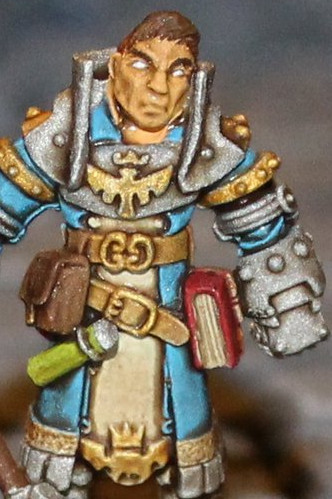
\includegraphics[width=2cm, height=3cm]{C:/privat/rpg/crimson_throne_book/latex/images/shaoban}};
	
		\node[below right,font=\bfseries\setmainfont{Immortal}\large] (name) at (0,0) {SHAOBAN};

		\node[below=of name.south west,below right,yshift=0.5em] (info){LN small human};
		
		\node[below=of info.south west,below right, align=left] (skills) {
                Init +0; Senses Perception +2\\ 
                Common
		};

		\node[below=of skills.south west,below right, align=left] (ac){
                AC 11, touch 11, flat-footed 11\\
                HP 5 (1HD)\\
                Fort -1, Ref +0, Will +2
		};
	

		\node[below=of ac.south west,below right, align=left] (fight) {
                Speed 30 ft. (6 squares)\\
                Melee dagger (small) +1 (1d3/19-20)\\
                Ranged dagger (small/thrown) +1 (1d3/19-20)\\
                Face 5 ft. Reach 5 ft.\\
                Base Atk +0; CMB -1; CMD 9
        };

		\node[below=of fight.south west,below right, align=left] (abilities) {
                Str 10, Dex 10, Con 8, Int 8, Wis 14, Cha 18
	   };

		\node[below=of abilities.south west,below right, align=left] (feats) {
                Simple Weapon Proficiency
	   };

		\node[below=of feats.south west,below right, align=left, text width=7.5cm] (skills) {
            Appraise -1, Bluff +4, Diplomacy +7, Disguise +4,\\ 
            Fly +2, Heal +2, Intimidate +5, Perception +2,\\ 
            Sense Motive +6, Sleight of Hand +6, Stealth +4,\\ 
            Survival +2
	   };

		\node[below=of skills.south west,below right, align=left, text width=7.5cm] (poss) {
            Dagger (small) 
	   };
	
		\node[below=of poss.south west,below right, align=left, text width=7.5cm] (traits) {
            {\itshape Child of the Streets:} {\scriptsize You grew up on the streets of a large city, and as a result you have developed a knack for picking pockets and hiding small objects on your person. You gain a +1 trait bonus on Sleight of Hand checks, and Sleight of Hand is always a class skill for you.}\\
            {\itshape Ease of Faith:} {\scriptsize  Your mentor, the person who invested your faith in you from an early age, took steps to ensure that you understood that what powers your divine magic is no different than that which powers the magic of other religions. You gain a +1 trait bonus on Diplomacy checks, and Diplomacy is always a class skill for you.}
        };
	\end{tikzpicture}
    \hspace{1cm}
    %%%%%%%%%%%%%%%%%%%%%%%%%%%%%%%%%%%%%%%%%%%%%%%%%%%%
    %%% Quintilian
    %%%%%%%%%%%%%%%%%%%%%%%%%%%%%%%%%%%%%%%%%%%%%%%%%%%%
	\begin{tikzpicture}[font=\footnotesize,node distance=0em]
		% Frame
		\fill[yellow!10, draw=black, rounded corners] ($(0,0) + (-0.25cm,0.25cm)$) rectangle (8cm,-12cm); 
    
        \node[below right] at (8cm-2cm-0.25cm-0.25cm,0) {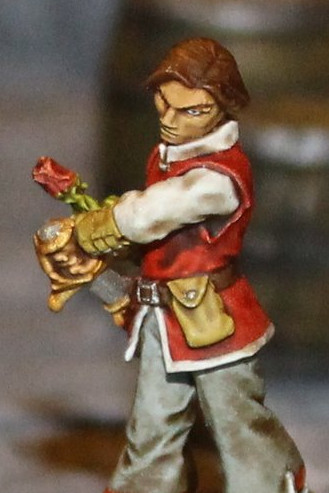
\includegraphics[width=2cm, height=3cm]{C:/privat/rpg/crimson_throne_book/latex/images/quint}};
    
        \node[below right,font=\bfseries\setmainfont{Immortal}\large] (name) at (0,0) {QUINTILIAN};

        \node[below=of name.south west,below right,yshift=0.5em] (info){CG small human};
        
        \node[below=of info.south west,below right, align=left] (skills) {
                Init +2; Senses Perception -1\\ 
                Common
        };

        \node[below=of skills.south west,below right, align=left] (ac){
                AC 13, touch 13, flat-footed 11\\
                HP 5 (1HD)\\
                Fort -1, Ref +2, Will -1
        };
    

        \node[below=of ac.south west,below right, align=left] (fight) {
                Speed 30 ft. (6 squares)\\
                Melee dagger (small) +1 (1d3/19-20)\\
                Ranged dagger (small/thrown) +1 (1d3/19-20)\\
                Face 5 ft. Reach 5 ft.\\
                Base Atk +0; CMB -1; CMD 11
        };

        \node[below=of fight.south west,below right, align=left] (abilities) {
                Str 10, Dex 14, Con 8, Int 14, Wis 8, Cha 16
       };
	\end{tikzpicture}
}

\resizebox{!}{\h\textheight}{
	\begin{tikzpicture}
		% Frame
		\fill[yellow!10, draw=black, rounded corners] ($(0,0) + (-0.25cm,0.25cm)$) rectangle (8cm,-12cm);	
	
		\node[below right] at (8cm-2cm-0.25cm-0.25cm,0) {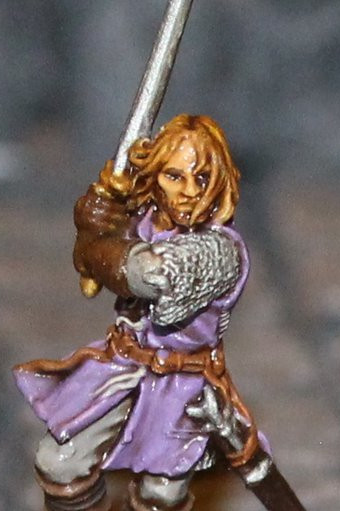
\includegraphics[width=2cm, height=3cm]{C:/privat/rpg/crimson_throne_book/latex/images/balian}};
	
		\node[below right,font=\bfseries\setmainfont{Immortal}\large] (name) at (0,0) {BALIAN};
		\node[below right] at (0, -0.45cm) {LN small human};
	
	% Init +0; Senses Perception +2
	% Languages Common
	% AC 11, touch 11, flat-footed 11
	% hp 5 (1HD)
	% Fort -1, Ref +0, Will +2
	% Speed 30 ft. (6 squares)
	% Melee dagger (small) +1 (1d3/19-20)
	% Ranged dagger (small/thrown) +1 (1d3/19-20)
	% Face 5 ft. Reach 5 ft.
	% Base Atk +0; CMB -1; CMD 9
	% Abilities Str 10, Dex 10, Con 8, Int 8, Wis 14, Cha 18
	
	
	
	\end{tikzpicture}
\hspace{1cm}
	\begin{tikzpicture}
		% Frame
		\fill[white, draw=none, rounded corners] ($(0,0) + (-0.25cm,0.25cm)$) rectangle (8cm,-12cm);	
	
		% \node[below right] at (8cm-3cm-0.25cm-0.25cm,0) {\includegraphics[width=3cm, height=4cm]{C:/privat/rpg/crimson_throne_book/latex/images/titlepage}};
	
		% \node[below right,font=\bfseries\setmainfont{Immortal}\large] (name) at (0,0) {PUK};
		% \node[below right] at (0, -0.45cm) {LN small human};
	
	% Init +0; Senses Perception +2
	% Languages Common
	% AC 11, touch 11, flat-footed 11
	% hp 5 (1HD)
	% Fort -1, Ref +0, Will +2
	% Speed 30 ft. (6 squares)
	% Melee dagger (small) +1 (1d3/19-20)
	% Ranged dagger (small/thrown) +1 (1d3/19-20)
	% Face 5 ft. Reach 5 ft.
	% Base Atk +0; CMB -1; CMD 9
	% Abilities Str 10, Dex 10, Con 8, Int 8, Wis 14, Cha 18
	
	
	
	\end{tikzpicture}
}
\end{center}

% \section{Test}
% \kant[1]

	%!TEX root = ../crimson_throne_book_main.tex
% 2013-05-19
\section{10 Erastus 4703}

It is still early in the morning when Hookshanks bursts through the door of the outhouse of the old clog shop, the abandoned building Lamm and his cronies have occupied as their home base. Hookshanks is a gnome, a mean little bugger, small even for gnome standards. With an evil grin across his face he singles out three of the lambs, Balian, Sjo and Quint. "Time to go hunting, you fools. Gobblegut's hungry. If you don't want to be the alligator's next meal, you'd better get him some juicy rats. Now move along!"\\

Hookshanks leads the three boys to the alley around the corner, using his rusted meat hook to pull open the grating covering the manhole to the sewers. "There are supposed to be at least ten rats for every Korvosan down there, so it shouldn't be a problem to secure a healthy catch. Four's a nice number, I'd say, so you bums don't even think about returning with less. Happy hunting, and don't let the sewer monsters bite."\\

Armed with a simple kitchen knife, the three youngsters descend into the damp darkness. A foul smell welcomes them. Clutching a fluttering torch, Balian lights the way. He spots a couple of rats further down the ledge, next to the filthy muck. Quietly the boys creep closer, only to suddenly jump the surprised rodents and take out two of them before the rest scurries off into a large drain. Sjo never gets in a blow, since the unfortunate soul slips before he can make it to the fight.\\

Across the sewage Quint notices a cul-de-sac that is blocked off with heavy metal bars. A couple of small drain pipes in the ceiling trickle down their smelly contents, while two more rats are chewing on some rotten left-overs against the back wall of the dead end. If only he could squeeze through the bars, Balian would easily add two more critters to his haul. After covering himself with filthy mud and slime, the boy manages to glide through the iron poles and using his torch as a two-handed club, he knocks out the rats. It's a dirty job, literally, but two and two make four.\\

Urged by Sjo the boys set off into another branch of the sewers and kill two more rats before returning to the surface. Today Hookshanks is satisfied with their work, so there will be no repercussions. The gnome does insist that the boys bear witness to the alligator's meal, however. In the flooded cellar of the clog shop, Gobblegut tears through the rats' cadavers in no time, reminding the young hunters that they would never want to switch places with the dead rodents.\\



	%!TEX root = ../crimson_throne_book_main.tex
% 2013-05-19
\section{11 Erastus 4703}

The next morning sees the three young friends on the doorstep of an abandoned theatre. This time they are joined by three fellow lambs, Edu and Lick, two fourteen year old boys, and the lambs' senior member, a kind girl of sixteen who goes by the name of Amarice. Overseeing today's operation are Lamm himself, his right hand man Yargin, a sour-faced wanna-be alchemist, and Lou, Lamm's personal bodyguard, a skinny, but lean swordsman.\\

{\itshape ``This place harbors our new goldmine''}, Lamm gloats as he knocked on the dusty door. {\itshape ``The three of you will go in first''}, he grins as he beckons Edu, Lick and Amarice closer. Yargin draws out two strange harnesses that he fits around the boys' necks. A leather skin has been stretched across a curved neck-sized wooden bracelet, leaving the inside hollow to form some kind of container.\\

{\itshape ``Inside this old theatre are dream spiders, creepy crawlies that are a bit bigger than the ones you are used to. We need you to milk them of their venom. Just let them bite into the leather and their poison will seep into the space inside''}, Yargin explains.\\

{\itshape ``Are you mad?''} Edu protests, only to be answered by Lamm's hard fist. {\itshape ``Bring their webs as well''}, Gaedran Lamm orders, as he shoves a blanket into Amarice's hands, {\itshape ``but be careful not to touch the silky threads, because they make you see strange things.''} He also hands the girl a lantern, before pushing the three guinea pigs into the main hall and quickly closing the door behind them. {\itshape ``Just give us a shout when you're ready''}, the old man mocks.\\

A few minutes pass before a burst of shouts erupts, followed by complete silence~\ldots Then someone pounds on the door: {\itshape ``Let me out! Let me out!''} It is Lick's voice. Yargin is in doubt: {\itshape ``What should I do, boss? What if there are spiders on the other side of the door?''} Since Lamm does not make a decision immediately, Sjo and Quint urge Yargin to let Lick out. The boy stumbles through the doorway, covered in cobwebs. As he faces Lamm, Lick falls back against the wall, warding off the old man while deliriously screaming: "Leave me alone, you nasty spiderman! He raises his arms in protection, but Lamm still hits him hard against the head, knocking him out. Lou swipes away the webs with his blade, noticing that the harness had not been pierced.\\

{\itshape ``A good thing we brought some extra fodder''}, Lamm remarks as he binds Lick's harness around Balian's neck. {\itshape Remember,''} he warns the boys, {\itshape ``do not touch the webs, unless you want to end up like this poor bastard.''} Then he shoves Balian, Quint and Sjo into the theatre.\\

The three boys look around anxiously. The former seating area stretches out before them, reaching a raised stage at the far end of the room. Toppled over benches are scattered across the floor, thickly covered in spider webs. Realizing they are unarmed, the boys tear off some planks from a broken seat, to use as makeshift clubs. Balian, who is holding the light, notices Amarice's abandoned lantern on the floor in front of the podium. There is no immediate sign of the two missing lambs.\\

While they are pondering what to do, a spider jumps out of nowhere and attacks the kids. The monster is huge, easily as big as a large dog. Swinging their wooden sticks, the boys quickly take down the arachnid, but not before it bites Sjo in his neck and shoulder. Part of its venom seep into the harness, but the Shoanti gets a serious shot of the poison in his shoulder as well, leaving him hazy and disoriented. While Sjo takes a minute to get his bearings, his friends successfully milk the dead spider's fangs for more venom.\\

Next the boys make their way to the stage. Dangling from the rigging above the podium is another spider. This specimen is so preoccupied with the cocoon it is weaving that it doesn't even noticed the kids approaching until Balian hammers it in the head. After defeating the spider, the boys cut down the cocoon and free their friend Edu from the webs. Before they are able to carry him off the stage, two more spiders leap down. One of them puts its fangs in Quint's leg and with only a wooden stick in their hands, the boys suddenly feel overpowered. Then a trapdoor in the floor of the stage bursts open and Amarice hops out. She knocks down one of the monsters, giving the boys a chance to finish off the other one.\\

After they have milked the arachnids of their poison, the lambs consider what to tell Lamm. The old man will not be pleased to learn that his goldmine has already run dry. If they lie and tell him the spiders are still alive, he will surely send them back in a few days and they'll be in all kinds of trouble then. So they decide to go with a colored version of the truth. Balian, who isn't such a schemer as his colleagues, strolls about on the podium while his friends are plotting. A smaller cocoon draws his attention when it quivers with a light spasm. Balian examines it and carefully unfolds the webs, discovering a black labrador puppy inside. The baby dog is still breathing, although it is unconscious, just like Edu.\\

Next the kids rejoin Lamm and his men, confessing that they have killed four spiders, but have at least managed to extract their venom. Moreover, they have seen lots of baby spiders inside, who will probably be full-grown in a few months. Sjo and Quint bring such a compelling version of the truth that Lamm completely buys it. They also manage to draw away the adults' attention from Balian, who is hiding the small pup under his clothes. On their way home Quint explains to Lamm how a small animal, like a rat, with a harness around its neck, would make for better bait than a human. Some kind of stuffed animal puppet might even be preferable. Lamm says he will consider this idea, but he doubts that much venom will seep into the container if no one is able to steer the bait.\\

Back in the clog shop the boys and Amarice are given the rest of the day off to recover from their ordeal. Although the kids decide that it won't be too hard to hide the puppy from Lamm and his men - the outhouse is big enough and the adults never come in for long - they do fear one of their own, Jecko, who has a rep for being a snitch. The boys try to come up with a suitable solution and also start to wonder what happens to lambs when they have ``finished'' their service to Lamm. Since none of their retired brethren have ever been seen or heard of again, they fear that riper teenagers are sold off as slaves to Cheliax, or even worse, killed. Amarice probably doesn't have much time left, since she's sixteen; it's her smallish stature that keeps her here for now.\\

When the other lambs return from their day's work, they convince the little traitor Jecko that ``Spyder'', as they dubbed the labrador pup, is their secret and that it will be Jecko's job to see to it that everyone keeps it.\\

That evening Sjo, Balian and Quint have to assist Lamm in the old shop. He is expecting a guest and needs Sjo and Quint to convince him the stupid neck harness plan didn't work and had almost killed them. Balian's job will be simpler, he'll be fetching food and drink.\\

Half an hour later the guest arrives. It is a truly ugly man, very skinny, with a crooked nose and a receding hairline. His skin is pale and blotchy from various scars. He's wearing a long leather apron that bulges with surgical tools and he has a chemical smell about him.\\

Lamm starts complaining how he almost lost a couple of his lambs to the dream spiders, but the guest, whose name seems to be ``Rolth'', tells Gaedran not to fret. He gladly collects the venom and the spider webs and hands Lamm a small bag in return. {\itshape ``I don't care how you get my stuff''}, the guest hisses, {\itshape ``we both know you love doing business with me if you can get Pesh for it. You'll let me know when you have more \ldots''} Then he leaves.\\

So this is what the boys have risked their lives for, Pesh. It is no secret that Lamm deals a bit of drugs now and then, but the lambs certainly do not feel it is worth their lives. Sjo swears he will make the old man burn in hell.\\



	%!TEX root = ../crimson_throne_book_main.tex
% 2013-05-19
Really like your "prelude sessions"! Nice foreshadowing here, as well! Keep up with it!\\



	%!TEX root = ../crimson_throne_book_main.tex
% 2013-05-26
% Wow, this is really good stuff. Your players will be a lot more immersed in the story when you begin the first adventure now that they've had an actual taste of Gaedren Lamm's evil.\\

% How are the mechanics for these young pre-adventurers working out for you? Did you take the adult version of the characters (level 1) and then applied some penalties to some stats, and made them of Small size?\\



	%!TEX root = ../crimson_throne_book_main.tex
% 2013-05-28
Thanks for the compliment. The prelude sessions serve to give the players a heart-felt hatred of Lamm, but also to make Korvosa feel more like home and to foreshadow some NPCs.The mechanics for the kid versions: Because of the simple weapon proficiency the PCs had a chance to hit something, so the fights that were actually very simple, were fun anyway. Still, enemies hit easily as well because of the low AC the PCs have. 

	%!TEX root = ../crimson_throne_book_main.tex
% 2013-05-29
Congrats on a very interesting idea !\\



	%!TEX root = ../crimson_throne_book_main.tex
% 2013-06-02
\section{12 Erastus 4703}

The Narrows of Saint Alika, the small channel between Endrin Island and mainland Korvosa, is famed for its tasty oysters. The mixture of salty sea water and sweet river water makes for an excellent breeding ground for the shellfish, providing both the perfect temperature and salinity.\\

Supervised by Lou the swordsman and Giggles the snickering half-orc, a dozen of Lamm's children have been diving into the murky water all day to locate and dislodge oysters. While Quint is struggling to meet the quota, Sjo and especially Balian do much better and have oysters to spare, dividing them among their closest friends to avoid punishment. Jules, an eleven year old lamb, is having an extremely terrible day. His weak constitution and a lingering cold have him slogging and cursing all afternoon. By the end of the day his hands are raw and cut, and he feels cold and out of breath. On top of that he gets a beating at the hands of Giggles for not meeting the required number of oysters.\\

When everyone stumbles into his cot in the outhouse of the clog shop that night, Jules is still cursing and swearing to finish off Lamm once and for all. Alika, who doesn't like bad language, closes herself off from his harsh words and occupies herself with her favorite pass-time, carving little wooden soldiers. Still, her hands are sore from farming oysters, so her efforts don't amount to much and she quickly joins the others in sleep.\\



	%!TEX root = ../crimson_throne_book_main.tex
% 2013-06-02
\section{13 Erastus 4703}

The sun hasn't risen yet when Balian wakes up. His little sister is talking to the pup Spyder: "Shht, be quiet ,Spyder. We have to be smart about it, not like those stupid boys. You have to stay here, no you can't follow them ..." If Balian asks Alika what's going on, she informs him that Jules and Jecko have left. They snuck out, first Jules and then Jecko. Spyder wanted to follow them, but Alika is keeping him here, because it's not smart to try and run away. Someone always ends up paying. Balian wakes up his friends, but before the boys can figure out a course of action, they hear heavy footsteps approaching their dormitory.\\

The door to the outhouse is flung open. Giggles tears into the room: "Ruaaah, wake up, little lambs, wake up! Outside! Now! Nooooow!" The kids scurry to the courtyard, where they come across a gruesome scene: Lou the swordsman is nailing Jules to the backdoor of the shop. Lamm and his men are gathered around him; Jecko is standing inside, trying to fade in the shadows as the first rays of sunlight hit the rooftops.\\

Lamm looks furious. He regains just enough control over his breathing to hiss between his teeth: "No one leaves without my permission. No one abandons me! This is what happens to little black sheep who think they can betray me! Observe and consider if this is what you wish for yourselves! And praise the gods, because if we hadn't caught this lousy deserter, one of you would be hanging here in his place!"\\

Lamm turns to face Jules. "So you think you've got enough heart to resist me?! I don't think so, dog!" Lamm pulls out his dagger and stabs the weapon into the boy's chest. While Jules gasps his life away, Lamm keeps carving, cracks open the boy's ribs and cuts out his heart. He holds up the bloody organ: "This is all the heart he has left! No one deserts me!" Then the old man barges into the clog shop.\\

The lambs are sent back into the outhouse, where they try to process what just happened. Alika is inconsolable and is shivering with fear and sorrow.\\

Sjo boils with anger, especially towards that little rat Jecko. But Quint serves as the voice of reason. He figures that someone else would have had to pay the price if Jules had gotten away, possibly Amarice, since she is the oldest. It is usually the oldest who is charged with the responsibility over the group and who ends up paying when things go wrong. So even though Quint doesn't like the fact that Jecko is a traitor, he has to admit that Jecko saved someone else's life.\\

An hour later Hookshanks Gruller enters the outhouse and addresses Sjo, Balian and Quint: "What's this, you lazy bums, you think you get the day off simply because one of you's dead? Come, there's work to be done!" The gnome takes the three boys to the courtyard and waves his hooked weapon at Jules' mutilated corpse. "Take it down!" Since Jules has been nailed to the door, there is no easy way to take him down, and the boys have to tear him loose. While the kids working, the gnome hums a popular nursing rhyme, slashing his hook around Sjo's and Balian's necks during the 'deadliest' parts of the song:\\

"On Croaker day, on Croaker day   On Croaker day, on Croaker day   Afterwards Hookshanks orders the boys to feed Jules' corpse to Gobblegut. The boys are disgusted while watching the alligator rip the body to pieces. Hookshanks adds to the drama by threatening Balian: "Maybe Gobble wants some more, what do you think? Or should we feed him something more juicy, like a little girl whose feeble attempts at labor will never be enough to pay off her father's debts? Har har har, pwak, pwak, you chicken, your day will come soon enough, mark my words! Now go and fetch the others, I've got some real work for you!"\\

The lambs have to sweep the city streets for the rest of the day, a simple job Lamm likes to perform for Korvosa once in a while. He's only paid a few pinch (copper pieces) for it, but it buys him a lot of goodwill, so his small-time operation is left in peace.\\

That night the three young friends contemplate what to do. Betraying Lamm to the Guard will not work, because the old man is not officially wanted. They could leave a trail while performing their own little crimes, but that would incriminate them as well. Moreover, if Lamm were to get wind of this treachery, his wrath would be terrible.\\

The lambs even involve Jecko into their conversation. When they confront him with the fact that he ratted out Jules, he defends himself, saying he saved their lives. Jecko is just being careful and refuses to pay for someone else's stupidity. He understands the urge to escape, but refuses to do so, because someone always pays. The only plan he has ever devised to escape Lamm's clutches, is befriending someone with means, who can buy his freedom. Lamm knows a good deal when he sees one, so if he was offered enough money to let a lamb go, he would definitely agree. And more importantly, no one would have to suffer or die. Sjo doubts Lamm will ever let anyone go, since he can't afford to have his victims freed. They could set up a lawsuit against him, providing personal testimony of Lamm's evil and illegal deeds. Jecko urges caution, he says that Sjo, Quint and Balian are in the typical age category when the lambs start thinking they can get out. He warns them to perish the thought, because no one has ever succeeded at this in over twenty years.\\

For now, the three friends decide to gather more information on the relationship between their captors. Maybe they can eavesdrop at night and find out who amongst Lamm's cronies doesn't fit in with the rest.\\



	%!TEX root = ../crimson_throne_book_main.tex
% 2013-06-02
\section{14 Erastus 4703 - Foundation Day}

That morning Lamm calls everyone into the courtyard. Flanked by his mates the old man is waiting for the children. "Today's party-time", he grins. "Today's Korvosa's 296th birthday! And obviously, little lambs, we'll be partying along!" Lamm expects an enthusiastic reaction, but when he doesn't get it, he shrugs and continues.\\

"Don't get too excited, you boneheads. Listen carefully. Today the king will make his annual visit to the Golden Market. The finest of Korvosa will celebrate and get very drunk. That means little alertness, but lots of money. That's how we like it! Spread out across town and pick as many pockets as you can. We will meet here tonight and you'd better bring me some hefty pouches! And of course, have a good time as well, it's a holiday after all." Lamm even manages a smile before sending the children off.\\

Although their master seems quite content now, Balian and his friends know that Lamm is one of the first to get drunk today and he expects his lambs to steal a serious amount of gold. If not, there will be hell to pay.\\

Sjo, Balian and Quint quickly make their way to the Golden Market. It is still early in the day, so the people who are visiting the market right now, are actually there to do some shopping. But since it is a holiday, the crowd is bigger than usual and also in a finer mood. Quint attempts some stand-up comedy, trying to weave the king and his harem into his jokes, but he makes only a few pinch. His efforts serve as a perfect distraction for Balian to pick some pockets, though. Seeing how well they have become at this job, the boys entertain the thought of building up their own private stash, in case they ever need it. They decide to hide it the sewers next to the old clog shop where they usually do their rat hunting. Especially the barred dead end would make an excellent hiding place, since the bars are only wide enough to allow a child to wriggle through.\\

By three in the afternoon the streets are packed with people who are psyched to see the king. The three boys have located a juicy target in the masses: Korvosa's magistrate of commerce, Garrick Tann, also known as the most hated man in Korvosa because he is in charge of taxes. Quint and Sjo move through the crowd to position themselves in front of the man, while Balian finds a spot behind the magistrate.\\

When the king comes into view on his beautiful black stallion, Sjo and Quint start screaming and jumping enthusiastically, distracting the man behind them. Balian seizes the opportunity to cut Tann's purse and also lift his dagger from its sheath. Then the boys sink into the crowd, trying to stay ahead of the approaching procession.\\

Although the monarch is getting older, he looks quite impressive in his ornamental gold breastplate and crimson cloak. The king is flanked by field marshal Cressida Kroft, the commander of the Korvosan Guard, and the seneschal of Castle Korvosa, Neolandus Kalepopolis. Twenty Korvosan guards on horseback fall back behind the trio and six members of the Sable Company keep a close watch from the sky, seated on the backs of their hippogryphs, much to Sjo's excitement, because the young Shoanti is fascinated by the black aviators.\\

Suddenly the crowd's cheering turns into a different kind of commotion. A beautiful young noblewoman on the other side of the street can't control her white mare and is thrown from the saddle. When the king sees her falling, he halts and slowly dismounts.\\

"By the gods," the king utters, reaching out his hand to the woman, "Shelyn truly blesses me today, what rare beauty crosses my path? Are you hurt, milady?"\\

"Lord Eodred, oh, I'm so ashamed. Forgive me for interrupting your procession with my clumsy behavior", the girl sighs. Her accent indicates she is from Cheliax.\\

"A welcome distraction on a boring day. Same show every year, put on a happy face and wave at the cheering faces. I know better ways to fill my days, but you know how it works: noblesse oblige and all that", the king confides. "Allow me to help you up."\\

"Oh, of course, silly me, I'm still lying in the dust in front of the king of Korvosa", the girl stammers. She elegantly reaches out for the king.\\

"You wouldn't be the first to crawl through the dust for me," the king smiles, "but in your case it's really not necessary. Would you do me the honor of joining me?"\\

"Oh," the woman blushes, "I'd love to, my lord." The crowd cheers when the noblewoman rides off at the king's side. While everyone is staring at the lovely couple, Quint's eye falls on something in the dust where the woman fell. He dives through the crowd and picks up a bejeweled brooch with a broken clasp. It is made of white gold and inlaid with small diamonds. There is an inscription on the back: "To my darling Ilie, dad". It must certainly be worth hundreds of golden sails.\\

When the king is gone, Sjo counts today's loot. Especially Tann's fat purse has given the boys a nice catch, over 12 gold pieces in value. On top of that they have a priceless jewel and a dagger that is expertly crafted.\\

The boys decide to hide the brooch and the masterwork dagger in the sewers and hand the money to Lamm, when he returns in the evening. Since there is no need to continue stealing, the boys enjoy the rest of the day off like normal children would. They also learn the name of the noblewoman who has enthralled the king: Ileosa Arvanxi from Cheliax.\\



	%!TEX root = ../crimson_throne_book_main.tex
% 2013-06-02
\section{30 Erastus 4703}

The next couple of weeks the lambs are kept busy. Sjo, Balian and Quint have to work in the harbor, cleaning the hulls of ships, an arduous and dangerous job.\\

The evening of the 30th Alika takes "The Korvosa Herald"' home, a printed newsletter that is published once a fortnight. She asks Balian to read it to her, while she starts carving another wooden puppet. The Herald announces the up-and-coming wedding of the king to the Chelaxian noblewoman he met in the market, Ileosa Arvanxi. The marriage is planned for the 31st of Arodus, on the holiday of Saint Alika. The back of the Herald traditionally covers a piece of history, focusing on Korvosa's early battles with the Shoanti. Sjo feels a bit sour when he learns that the Sable Company was founded by a handful of veteran soldiers who had survived the Shoanti attacks. By the time Balian has finished reading, he sees the sculpture his sister has carved: the new queen.\\



	%!TEX root = ../crimson_throne_book_main.tex
% 2013-06-02
Nice introduction for the queen and her brooch there. :)\\



	%!TEX root = ../crimson_throne_book_main.tex
% 2013-06-03
Did you give to your players a handmade copy of the Korvosa Herald ? Labor of love, indeed !\\



	%!TEX root = ../crimson_throne_book_main.tex
% 2013-06-03
Yes I did, they will get one every two weeks.\\



	%!TEX root = ../crimson_throne_book_main.tex
% 2013-06-15
% DM's note:\\

% The following session was based on the module 'Murder's Mark'. The adventure itself has been cut down to a much shorter version, keeping the carnival and the murder, but leaving out all the extra encounters and combats, since my 0-level PCs are not up to such challenges yet.\\



	%!TEX root = ../crimson_throne_book_main.tex
% 2013-06-15
\section{20 Arodus 4703}

Hookshanks walks into the old clog shop, obviously in a good mood. He hands Lamm a flyer, telling him a nice opportunity has presented itself. The Umbra circus has come to town. They arrived yesterday and set up camp in Endrin Square in the East Shore district. A circus is the perfect place to pick pockets: easy targets and suitable scapegoats, because the carni's will most certainly be blamed for everything that goes wrong or gets stolen.\\

Lamm sends out Balian and his mates to Endrin Square because the boys performed so admirably at the golden market recently. He expects them to come home with fat loot and the children know their master is not easily satisfied.\\

The Umbra carnival is a colorful collection of circus wagons and tents. The boys, who have no money to pay the admission fee, sneak in undetected and gaze at the wonders of the carnival. Playful music drifts from a barrel organ, its sharp tones cutting through the hum of the crowd. Dozens and dozens of Korvosan citizens roam around to play at the high-striker game, have their fortune told or visit the magnificent Madame Mask. While mothers wave at their children on the carousel or take them to brave the baby dragon, fathers gather at the bar to get drunk, hoping their wives will leave with the children before the nightly peepshow starts. Still, the highlight of the circus is an enormous tent that opens only twice a day. A painted sign at the entrance announces a mythological animal with a capricious nature that offer riddles to be solved: a sphinx! Two carni's stand guard at the door.\\

Some early visitors to the fair have already started drinking at the bar. Quint and Sjo provide a distraction, allowing Balian to lift a hefty pouch, the first catch of the day.\\

Later the boys walk into a large and brightly colored pavilion tent to watch the show of Madame Mask. Three runways lead to a raised dais with a tall rectangular box, covered on all sides in mirrors. A nimble carni makes his way through the crowd to collect 5 pinch from every visitor: "Stare at Madame Mask's curves and make some money. Only five pinch! The fastest eyes win the pot!"\\

Then a beautiful woman with a silver mask strides into the tent. She uses the central runway to walk up to the dais. She doesn't talk, but nods and waves at the visitors. Her shapely body is covered in a risqu\'e blue gown. She is also adorned with various scarves, all kinds of jewels and flowers in her hair. She sends a few charming smiles into the audience before stepping into the mirrored box.\\

"I hope you've been paying close attention", the gypsy who collected the money shouts. "Now's your time to prove it!" Three doors open in the cabinet and three ladies step out. They are all Madame Mask, but each of them is dressed differently. "Each Madame Mask wears a different outfit from the original, but each of them wears a single piece that the original was wearing as well. The first one to identify all three items wins this money", the crier clarifies, holding up the sack of money.\\

The public stats shouting the names of all the items and accessories the women are wearing. The crowd quickly picks up on the white rose, woven into the left Madame Mask's hair, but it takes the young lambs a few breaths longer to lay their finger on the other two items: a fine silver chain around the waist of the lady in the center and a silver ankle bracelet on the beauty to the right. The prize money amounts to a little over two gold sails.\\



	%!TEX root = ../crimson_throne_book_main.tex
% 2013-06-15
After the show the youngsters realize that the excitement made them forget to do their jobs and pick pockets. They decide to make amends and join a crowd that is gathered around a carni who's juggling burning torches and breathing fire. Balian lifts another pouch, but when he examines it, it turns out to be a meager catch of one silver shield and a couple of pinch. Suddenly a hand seizes Balian by the collar. A blue-eyed gypsy holds the boy in place with his firm grasp. "Excuse me, young man, master Terdal would like a word with you." The man is quickly joined by his colleague from Madame Mask's show. When the boys get ready to resist, the blue-eyed carni quickly pulls out a knife, which he gently places on Balian's throat. "I have no intention of hurting you, boy, if you just come along. All we want to do is talk." The lambs realize they are outmatched and follow the gypsies to a barrel-shaped wagon, where an older carni with a patient face kindly invites them to take a seat.\\

"Hello, my name is Alan, Alan Terdal", he says. "My companions have noticed your little ... antics, shall we say. You do understand that we can't have anyone picking pockets at our fair. It reflects badly on my kind, I'm afraid. So what shall we do with you, it would be a pity to hand you over to the guard, now wouldn't it?"\\

At first the boys are not inclined to negotiate, but when they finally agree to return the stolen money, Alan nods approvingly and makes them an offer. A Varisian circus like his is perpetually plagued with a bad rep for deception and petty theft, no matter how honest the carni's really are. Alan asks the lambs to act as his eyes and ears in the crowd, picking out other pickpockets from the visitors. He's even prepared to pay the boys for their services. When the youngsters agree, Alan impresses on them not to interfere themselves when they spot a thief, but to warn him or his companions, Jonah Blue-eye or Landro the Fiddle. The boys can also eat and drink for free or participate in any of the attractions.\\

Balian, Quint and Sjo enjoy the rest of the afternoon at the fair, eating and drinking as much as they want, but keeping their eyes open at all time. When Balian plays at the high-striker game, he smashes the heavy wooden mallet on a lever to sends a puck up to a lion's head on a pole. The puck fails to meet its goal and the head does not roar, as it did with the previous contestant. Instead it simply meows and licks its lips, to the amusement of the bystanders.\\



	%!TEX root = ../crimson_throne_book_main.tex
% 2013-06-15
At 4 o'clock the doors to the Sphinx's tent open. The pavilion leans against a large wagon with an iron cage. Visitors gladly pay the one silver shield admission price for a chance to gawp at this creature of mythology. Two guards keep the visitors under control, preventing them from touching the curtains that cover the cage.\\

Alan Terdal welcomes the guests: "Ladies and gentlemen, what you're about to behold is something most of us can only dream about. The searing sands of far-away Orision are home to a fabled creature, half woman and half lioness. This sphinx is a marvel indeed, wonderful but capricious in nature. That's why we disturb her rest only a few times a day, but be warned, for if you do not succeed in solving her riddles, she might lose her patience ... Still, guess what she's describing and you get to plunder her treasures! So without further ado, here is Jherizhana, the sphinx" The gypsy pulls a cord and the curtains slide open.\\

Behind the bars of the cage stands a beautiful sphinx, surrounded by satin cushions and silk sheets. She shifts about nervously until she finds her peace, looks into the spectators' eyes and melodiously recites her riddle:\\

"At the sound of me, men dream or stamp their feet,  The visitors and the three lambs start shouting all kinds of wrong answers, obviously irritating the fierce lioness, who begins to pace from left to right and repeats the riddle twice, each time with less patience in her voice.\\

Suddenly Quint has an epiphany and cries out the solution: "Music!" The expression across the sphinx's face softens immediately. She beckons the young lamb closer and invites him to open one of the chests in front of her cage. Quint picks the fourth chest from the left, in which he discovers a small ball of golden cheese, a true delicacy for malnourished lambs.\\

Meanwhile Balian and Sjo notice a man who's trying to glide through the crowd, paying more attention to the visitors than the creature in the cage. The man spots a juicy target and lifts his purse during the highlight of the show, when Quint solves the riddle and the bystanders applaud his success. Sjo alerts Jonah, who signals Landro to intercept the thief. The pickpocket turns out to be one of the Szcarni, a gang of Varisian mafiosi who live in the poorer outskirts of Korvosa.\\

Alan's daughter Liandra returns the stolen pouch to the victim, a barrel-bellied man with grey sideburns and a cordial smile. She invites the lambs to come over and introduces them to the victim, Ausio Carowyn, the head of a minor noble family. He praises the youngsters for their honesty and awards them a gold sail each for their help.\\

At the end of the day the boys get even more money from Alan, who invites them to return the next day and continue their good work. The boys made a little over 9 gold sails today with mostly honest work. They have eaten well and had a very enjoyable day. They turn over 6 gold pieces and some petty chance to Lamm, storing 3 gold sails in their secret stash in the sewers. When they get back to the outhouse, they share the cheese with their friends.\\



	%!TEX root = ../crimson_throne_book_main.tex
% 2013-06-15
\section{21 Arodus 4703}

When Balian and his mates return the next day, they aren't allowed inside the circus grounds. The Korvosan guard is preventing anyone from entering or leaving the site. The bystanders are whispering that someone was murdered here last night, but no one knows any specifics.\\

The boys decide to sneak in the same way they did the day before. Sjo and Balian hide in Alan's wagon, while Quint uses prestidigitation to color his shirt brightly, making him look like a carni kid. He singles out Alan and waves him over to his wagon. The carni is relieved to see the lambs: "My young friends, I'm afraid I have some bad news. Someone was murdered here last night. The carnival is closed and one of us is under suspicion of the vile crime: Jherizhana, our sphinx. The victim appears to have been wounded by heavy claws. And to make matters worse, our 'bird' has flown: Jherizhana is missing. "\\

"Still, I'm absolutely convinced that Jherizhana is innocent. Don't ask me how I know, but trust me, I'm 100 % sure. My fellow carni's and I have been grounded, so I would like you boys to investigate the matter for me. Would you be prepared to help us out? If you can prove our innocence, I will reward you handsomely."\\

When the three boys agree, Alan continues: "The man who was murdered last night, was named Boris Veldan, a local moneylender and pawnbroker. He had been drinking heavily at the bar yesterday and was murdered later last night in another corner of the camp, behind the cage of the baby dragon and Madame Mask's tent. Apparently he had been ripped to shreds.\\

That is exactly why Jherizhana is a suspect, because the wounds on Veldan's body appear to come from her claws. Lieutenant Jalento of the guard, who's leading the investigation, seems to be convinced of her guilt. Moreover, the sphinx is no longer around, which only adds to the suspicion. Maybe her magic foresight warned her and made her fly off ... I'm not sure, but she has disappeared at a most inconvenient time.\\

Jherizhana would never hurt a fly, she's incapable of doing so. Her cage is only for show. I don't know why that Boris guy was murdered. Perhaps he was robbed, because his purse is missing. Or maybe the Szcarni had a score to settle with him. Those damned gangsters give all my fellow Varisians a bad name. This moneylender might have been a thorn in their side ... well, I just don't know, I'm not familiar enough with this city. I hope you can figure out what happened.\\

Lieutenant Jalento let slip that this Boris Veldan owns a pawnshop close to the Dwarfwalk gate. Maybe you can start your investigation there."\\



	%!TEX root = ../crimson_throne_book_main.tex
% 2013-06-15
The three boys take the road north, towards the Dwarfwalk gate. On the corner of Kroft Boulevard and Threemast Street they see the pawnshop, 'The Hefty Purse'. It is a sturdy stone building. In front of the shop is a small group of people. Five guards are talking to a grieving woman and a frowning man in chain armor. A child is standing behind the woman. When the woman notices her son listening in on the conversation, she gives him a hug before asking him to go and play while she's talking to "these gentlemen".\\

The child shambles down the street, where Balian, Quint and Sjo approach him. His name is Bastian Veldan. His father was murdered last night at the circus and his pouch and keys were stolen. His father's body has already been taken to the Gray District, where the priests of Pharasma will bury him.\\

His dad bought things from people who needed money. If they didn't buy it back within a certain time span, his father could sell these things off to someone else, Bastian says. The man in chainmail, next to his mother, is Gerbrand, the head of security in the shop.\\

The woman calls out for her son to join her and the guards to the Gray District and greet his father's remains. The head of security accompanies them as well, leaving the shop in the hands of one of his agents. After the woman closes the shop, the party leaves.\\

A couple of minutes later a shifty character sneaks up to the shop. He scans the street and pulls out a key ring, trying several keys before opening the door and entering. The lambs wait for a couple of minutes, before they move over to the pawnshop and peek through the window. They see a dead guard lying on the floor in a pool of blood. The youngster wait for another ten minutes. Then they see the burglar coming out again with a leather satchel around his shoulder. A severe limp betrays the fact that he is wounded. He scurries down an ally, making his way to a rundown sailing boat in the Eastshore docks.\\

Sjo and Quint alert two soldiers from the Korvosan Guard who are patrolling the harbor, informing them that a murderer is hiding on a boat close-by. The two guards, a man and a woman, accompany them to the ship and order the man to come out, before kicking in the door to the cabin. Sjo gets a better look at the man now: he is pale and skinny, has blood on his clothes and heavy bags under his eyes. He's still trying to get up from behind the table, seizing a bloodied garden hook in the process, when the guards burst in and knock him out cold.\\

Next they examine the cabin. The leather satchel is on the table and contains several items of jewelry. There is also a scroll on the table, which bears fresh bloody fingerprints. It's the deed to the ship, which is the property of Verner Salor. The blood on the garden claw looks fresh as well. The guards don't seem surprised when they find drugs on the table. Judging from the man's physical state, he is most likely an addict.\\

The female guard figures the man is a pesh addict, who pawned his ship for a loan, so he could sustain his addiction. When he couldn't pay back the money he owed, he must have killed the pawnbroker.\\

The two guards join the lambs to the Umbra Carnival, where they easily convince lieutenant Jalento that they have caught the real killer. Alan Terdal is very happy that the carnival's name has been cleared and invites the lambs into his wagon to thank them. He also confesses that Jherizhana, the sphinx, doesn't exist: she is just an illusion conjured by his daughter. That is why the sphinx could be the killer. When Alan tells the kids that the circus will probably be closed for a few days, out of respect for the man who was murdered, he notices that the youngsters are disappointed. When they confront him with the horror of their master, Gaedran Lamm, the old Varisian feels for them. Although he can't make any promises, Alan assures the boys that he will look into the case more closely.\\

He also hands them a magic wand, which holds cure spells. He suspects the lambs might have need of it from time to time. The gypsy is happily surprised to find out that Balian, Quint and Sjo all possess the magic inclination to activate the wand. When he sends the boys off, their predicament is still mulling through his mind.\\



	%!TEX root = ../crimson_throne_book_main.tex
% 2013-06-16
It must be tempting for the kids to just leave Lamm's clutches and join the carnival. :)\\



	%!TEX root = ../crimson_throne_book_main.tex
% 2013-06-16
% It is, but they know that at least three of the other children will pay with their lives for their desertion, so unless they can get all 30 children out at once, it is a flawed plan.\\



	%!TEX root = ../crimson_throne_book_main.tex
% 2013-06-23
% Good point! :)\\



	%!TEX root = ../crimson_throne_book_main.tex
% 2013-07-21
\section{22 Arodus 4703}

The lambs spend the day in the Narrows of Saint Alika, working in the oyster beds. After a tiring day the kids are trying to catch their breaths over a plate of porridge in their dormitory. Yargin walks in, followed by Gaedran Lamm and a 'stranger', Alan Terdal, the leader of the Umbra Circus.\\

"Good evening, children. Allow me to introduce myself. My name is Alan Terdal. I'm a carnival artist and actor by profession. As you probably know, we're only a few days away from the birthday of Saint Alika and the king's marriage. In honor of the holiday and the wedding my group's planning a theater play, 'The Pied Piper of East-Rikkan', a lovely tale about a rat plague in a small Chelish town. I hear that Korvosa has its fair share of rats herself, so this piece might be enjoyed here.\\

We do have a problem, however, because the children of East-Rikkan play an important part in the story and since my group consists almost exclusively of adults, we're in dire need of some children. The kind mister Lamm here has allowed me to hire some of you. I'll be needed a dozen or so of you. Who would like to participate?"\\

Yargin immediately adds: "This play is by no means a way to escape your daily chores. Daylight hours are still for working. You can practice in your own time, in the evening! And those of you who'll be joining me in the country, come tomorrow, you're out! We'll be sleeping on a farm outside of the city, so we won't be around to play the fool on stage."\\

Almost all the lambs raise their hands. Yargin immediately rules out the smaller children, who will go to the countryside with him to pick baskets full of flowers for the feast of Saint Alika. This also excludes Balian's sister, Alika. In the end eleven lambs are chosen, including Balian, Sjo and Quint, but also Jecko, Edu and Lick. Alan Terdal convinces Lamm to let him take the children tonight already, for their initiation into the world of acting. The old miser agrees on one condition, Hookshanks Gruller, the gnome, has to join the play as well to keep an eye on the kids.\\

When the troupe arrives at the circus on Endrin Square, Alan's daughter Liandra welcomes everyone with open arms and immediately serves a decent meal to the skinny lambs. To learn the basics of acting, the children have to do some basic theater exercises, like acting out emotions, mirroring someone else's actions, practicing different ways of walking or improvising various characters who meet by accident on a steps of the temple. Some of the gypsies join in the fun, including Eran, one of the two children in the circus troupe. Although the six-year old is younger than any of the lambs present, he's already a fine actor and he actually gives the budding performers tips.\\

Sjo, Lick and Quint turn out to be naturals. Balian struggles a bit more, but no one is as bad as Hookshanks, who claims this acting business is plain stupid. The gnome refuses to fully commit to a role, fearing he will make a fool of himself, but his reserve only results in an even worse performance. The kids also employ every opportunity to make fun of the gnome. In all, the children have a great time and when they finally return to bed, their dreams are sweet for once.\\



	%!TEX root = ../crimson_throne_book_main.tex
% 2013-07-21
\section{23 Arodus 4703}

Early in the morning Yargin leaves with the younger lambs for the countryside. There they'll be picking red and white flowers for a week, that will traditionally be used on Saint Alika Day. Although Balian's sister will be joining Yargin, which means she won't get to play in the Pied Piper, Balian feels happy for her. This week outside of the city is usually quite enjoyable. The little lambs even think of it as their annual holiday.\\

The older lambs spend the day in the water again, diving for oysters and turning them in their beds, so they can grow larger by the end of the month.\\

That evening they are exhausted, but eager to visit the circus again. Alan asks Hookshank not to give the children dinner anymore. He will feed them during practice instead. This way they will save time, the old Varisian explains. Realizing how tired the children truly are tonight, Alan calls for food, drink and blankets. Everyone gathers around the campfire. Landro plays his fiddle while Alan tells the story of the Pied Piper.\\

Once upon a time there was an infestation of rats in the Chelish town of East-Rikkan. The desperate citizens hired a musician who claimed he could get rid of the rodents. Playing his flute, the Piper led all the rats to the river, where they drowned.\\

When the mayor refused to pay him, the musician grew angry and played his instrument again. This time the town's children followed in his wake and disappeared inside a mountain, never to be heard from again. Only two children remained to tell the tale. These two couldn't keep up with the others because one of them was a cripple and the other one hit his toe. Apparently Sjo and Quint will be playing those two roles.\\

Oyster farming and theater practice continue for the next couple of days, giving Quint and his mates some skill in acting.\\



	%!TEX root = ../crimson_throne_book_main.tex
% 2013-07-21
\section{31 Arodus 4703}

Saint Alika's Birthday is a holiday the lambs generally enjoy. They are never made to pick pockets, because Lamm opens up an oyster bar in front of the old clog shop. His children have to help him here. Lamm's superstitious nature somehow makes him believe that thievery doesn't fit in with the modest remembrance of Korvosa's selfless heroine Saint Alika. Still Lamm is not one to pass on an occasion to make money, which he does through selling oysters and wine.\\

The clog shop's central location makes it an excellent spot to participate in the festivities. Lamm has occupied most of the street in front of his home with tables and a large stall. He expects to do extra well this year because of the royal wedding. He also got hold of four free barrels of wine, a royal gift which are to be distributed for free. Being the business man he is, Lamm watered two of these down to four, keeping the remaining two barrels as his 'own' supply. He'll be offering these to paying customers.\\

The weather is excellent on this joyful day. In the morning Yargin returns with the smaller children from their 'holiday in the country', while the others are setting up Lamm's oyster bar. By noon most people leave for the Heights, hoping to catch a glimpse of the married couple at Castle Korvosa. Quint and Sjo beg Lamm to let them go watch as well. Since the old man is curious himself, he agrees, leaving Giggles behind to watch the shop and bar.\\

A vast crowd of Korvosans has made its way to the Heights, pushing and shoving to find a decent spot along Ramp Boulevard or on one of the streets surrounding the castle. Balian, Sjo and Quint climb one of the houses close to the castle to enjoy the spectacle from their 'front row seats' on the rooftop. At one o'clock all the bells in the city toll. The people cheer as the king and his new bride appear on the balcony to greet their subjects.\\

Trumpets blare and drums roll as a military parade makes its way along Ramp Boulevard from Kendall Plaza in the south. The soldiers halt in front of the castle, while fifteen hippogryphs fly overhead in a heart-shaped formation, strewing down red and white petals.\\

Field Marshal Cressida Kroft rides to the head of her troops. With a magically enhanced voice she speaks: "Your majesty, the Korvosan Guard salutes you and congratulates you on your wedding. We welcome your beautiful bride, our new queen Ileosa! (The people cheer.) To show our honor and loyalty, we would like to present her with a gift, her own private guard!"\\

At that exact moment the front ranks split and ten women in plate mail step forward. Their helmets are adorned with red plumes. "Behold!" Cressida Kroft shouts, "the Gray Maidens!" Another cheer arises from the masses. The king and queen nod their heads in approval as the Field Marshal orders her troops to move forward.\\

When the royals go back inside, the lambs hurry back to the old clog shop to work. Hookshanks is in charge of opening the oysters, the girls pour the drinks and the boys serve the patrons. Soon all the seats are taken. The free wine flows bountifully, but the oysters and housewine also move well, even though customers have to pay for them.\\

Twice Hookshanks cries out triumphantly as he finds a pearl in an oyster. He proudly hands the precious stones to Lamm, who tucks them away in his chest pocket. Several nervous looking people approach Lamm in the course of the day to buy tiny pouches. Many of his customers are young adults and most of them are decently dressed.\\



	%!TEX root = ../crimson_throne_book_main.tex
% 2013-07-21
By seven o'clock the lambs leave for Endrin Square, where the circus has built a spectacular stage. Giggles remains behind with a skeleton crew to man the oyster bar. The boys and girls are excited, although some of them are plagued by nerves. The Varisian actors welcome their extra's with open arms. Alan informs them that he has found real rats for the show, so there will be no need for magic tricks and illusions to conjure an army of rodents. He also introduces the kids to an elderly lady with a yellow sheen in her eyes, Meep Gildenglare. Meep will be sitting under the stage to handle the rats. Alan warns the kids to leave the woman in peace so she won't lose control over her animal friends.\\

By 7.45 Jonah jumps on stage, dressed as the mayor, and addresses the crowd: "Dear people of Korvosa, ladies, gentlemen, boys and girls, he- and she-rats, baby rats and elderly rats, I bid you all welcome! For, if I'm not mistaken, this city counts a fair number of rodents amongst its inhabitants. Well, let me put your minds at ease, it can always get worse. Because once upon a time in East-Rikkan, a small town north of Westcrown in Cheliax, there lived rats ... a great many rats."\\

And so the play begins. The lambs can watch from backstage how the story unwinds, occasionally stepping onto the podium themselves to join in the action. Sjo has to jump round in a state of panic with a rat on his back and Eran, the small circus child, plays an endearing boy who begs his mother and beckons the gods to 'please get rid of the rat problem'. The rodents themselves enter and leave the stage through some holes in the floor. Sjo notices Meep's yellow eyes burning down below through the cracks and he hears her whispering to the animals in a peeping voice. Quint and Lick are also intrigued by the mysterious woman and dare the young Shoanti to sneak a peek under the stage.\\

When Sjo slips down to spy on the old lady, he's surprised to see a tail sticking out from under her skirt. When she turns to face him, his heart skips a beat: her face has morphed into the features of a rat. Apparently she is one of those dreaded 'wererat' creatures. Sjo quickly runs off to inform his friends of his discovery.\\

Meanwhile Alan is on stage, pleasing the people with his role of the Pied Piper. He pipes a light-hearted tune on his flute, apparently making the rats obey his every wish. The spectators applaud the rodents' antics. When the rats have been disposed off, the good people of Rikkan refuse to pay the piper. The children are up next. They follow the musician in a dancing queue and disappear behind a waterfall. Two of them are late, Quint and Sjo. Their stumbling and fumbling sends roars of laughter through the crowd.\\

When the show has finished, the lambs share in the joy of being applauded and cheered. Alan thanks all the kids and Liandra gives them each a kiss on the cheek. She also slips a gold sail into Sjo's and Quint's hand, to thank them for their excellent performance.\\

Shortly after the play the lambs return to the old clog shop to continue working at the oyster bar. Even after the sun has set the seats are still filled. Lots of alcohol has flown and many of the customers are drunk, as is Gaedran Lamm. When darkness has truly set in, fireworks light up the night sky. The spectacle ends with a series of heavy bangs and flashes, which blaze up in the shape of an enormous woman holding aloft a wand. She represents the gargantuan statue that once stood over the harbor, on top of the Gatefoot.\\



	%!TEX root = ../crimson_throne_book_main.tex
% 2013-07-21
By midnight the oyster bar has completely sold out. In other parts of the city the feast is still in full swing. While Hookshanks and Giggles order the lambs to clean up, Gaedran invites Yargin and Lou for a trip around town. He charges Quint, Sjo and Balian to get three heavy chests from the front room and join them. The chests' marks have been burned away, identifying them as stolen goods. The boys have to be extra careful with them because their contents are extremely fragile.\\

Before they leave, Lamm goes inside to conclude some business, but the boys cannot make out who is in there with him. When he comes out, they leave for a bar in Midland harbor. On the way Yargin, who is quite intoxicated, bumps into Balian. The young boy stumbles but manages to hold on to his chest. Yargin is furious anyway and blames Balian for his incompetence.\\

In the bar Lamm and Yargin start gulping down a few pints of ale, though Lou abstains from alcohol, as usual. A few beers later a broadly smiling captain approaches. He exchanges a few words with Lamm, opens up one of the boxes and admires the ceramic plates inside. Then he has three of his men take away the merchandise, while handing Gaedran a pouch.\\

Gaedran and Yargin continue drinking heavily, while a kind barmaid gives the three boys in their company some milk and cookies. Lou tries to chat her up, but she skillfully wards off his advances. When Gaedran and Yargin are completely wasted, they join their customer, captain Korbat, and some other patrons in a game of chance. Lamm loses big. While his pile of coins slinks away, his temper rises. After having cleared Lamm of all his money and his last bag of drugs, captain Korbat prepares to leave. Lamm begs him for one last chance: "C'mon, cap'n. Give an old geezer one more shot. All you've taken from me against the boy!" Lamm points at Balian. "He's turning into a strapping lad, an excellent acquisition for your oars. Please, one more shot!"\\

The captain inspects Balian and answers amiably: "You've got yourself a deal, mister Lamm." He pulls out two dice. "Let's keep it simple; the highest roll wins."\\

Lamm throws the dice first. Double five! "Hah, ten! Try beating that, buddy!" Korbat takes the cubes and gently blows over them. "For chance." Quint watches him closely, trying to spot if the sailor is cheating, but he notices nothing out of the ordinary. Then Korbat throws the dice on the table. It's a double six. "Consider yourself beaten, old man." Three of his men jump up and grab Balian by his arms, dragging him outside. Lamm snickers in his seat: "You've brought me nothing but ill luck, boy! Good riddance!"\\

Then he claws at Quint's shirt: "Take me home, kid." Sjo is flabbergasted by what just expired and refuses to accept it. He swings at Lamm with his fist, hitting the old man in the face. His anger makes his hand burst out in sparks of fire. Meanwhile Quint tries to move towards the door, to follow the sailors who are carrying off Balian. Lou charges him and knocks him out with the flat of his sword. Sjo is also outmatched, getting cut by Lamm's dagger and receiving two splashes of acid in his face from Yargin's wand. While the acid burns in his eyes, he loses consciousness as well.\\

Quint awakens in the street when Lou empties a bucket of water in his face. Lamm and Yargin, who are both struggling to stand in their drunken stupor, order him to carry Sjo's unconscious body. But the Shoanti boy is big and heavy, and Quint can hardly support his weight, let alone move him. Yargin pulls out his wand again, threatening to burn the poor boy if he doesn't hurry up. Quint feels hopeless and pours all of his emotion into his hands, which suddenly glow with healing magic, restoring Sjo to consciousness. The Shoanti boy wakes up, but his sight is still blurry. Meanwhile Lamm and Yargin have grown tired of Quint's stalling and move forward to channel their frustrations on the boys once more.\\



	%!TEX root = ../crimson_throne_book_main.tex
% 2013-07-21
"Stop this madness!" A calm but determined voice sounds from up above. Staring at the rooftops, Lou makes out the outlines of a cloaked man. His face is covered by a scarf. "Blackjack", Yargin moans, staring up at Korvosa's caped crusader.\\

Lou draws his blade. Lamm reaches for his crossbow but he is too drunk to cock it: "You dirty dog, no one orders me around. Just you wait ..." The mysterious hero somersaults down, landing next to Lou. The bodyguard lunges at the rescuer's back with his longsword. The vigilante ducks under his fierce swing: "Good sir, I have no wish to harm you. Just let these children go."\\

"I will be known as the man who killed Blackjack", Lou crunches as he swings at his opponent once again. Blackjack parries his hits easily: "I hate to repeat myself. LET (woosh, he cuts Lou's cheek) the CHILDREN (woosh, he wounds Lou in the shoulder) GO (stab, he hits Lou painfully in his side)!"\\

"Last chance to abort the fight", the masked man warns his assailant. Still, Lou refuses to quit and strikes wildly at Blackjack, who spins around, letting the longsword cut through the air beside him. Then he slaps the hilt of his rapier against Lou's hands, easily disarming the man.\\

"And now you will let these children go!" Blackjack pronounces each word carefully to let them sink in. He doesn't wait for the thugs to reply, but pulls the children up and pushes them towards safety. Lou uses the distraction to draw his dagger and lunges forward. Blackjack bends through his knees, swinging his own blade under his arm so it sticks out like a sharp thorn from his back. Lou sees his surprise attack transformed into a fatal rush toward the deadly point. Unable to stop his momentum, he throws himself on the blade. He drops down, dead.\\

"Now quickly, follow me!" Blackjack doesn't waste time and leads the children through a maze of alleys, until they reach a quiet spot on the docks. There the boys fill their rescuer in on what happened and urge him to help them free the other lambs from the old clog shop. If they don't, Lamm will make the remaining children pay, most likely with their lives, as retribution for their little rebel friends.\\

Blackjack immediately agrees to help. They hurry to the shop, where Giggles and Hookshanks are still up, catching a few more drinks in the front room. Blackjack knocks them out easily, while Quint and Sjo collect the lambs from the outbuilding. When the children learn they are free, the scurry off into the streets. Lick has more bad news: Balian's sister Alika is gone. The pale and blotchy alchemist who deals drugs with Lamm and who bought the dream spider's poison, came by and took the girl in exchange for more of the mind-numbing merchandise. Quint remembers the creep's name: Rolth. Blackjack has heard of him as well, but says no one knows where to find the man.\\

Then Lick urges his friends to leave the room. Sjo sees a flicker of madness in the boy's eyes, as he takes a lantern and drops it on the floor. The rugs catches fire and the last lambs run out of the house. Lick has the puppy Spyder under his arm. He nods at his rescuers before disappearing into the city, while the clog shop bursts out in flames.\\

Quint and Sjo hurry to the docks, in the hope of finding Balian, but captain Korbat's ship has already left. Blackjack asks the boys if they have some place to go. They want to try their luck in the Umbra Circus. Alan Terdal welcomes them with open arms and agrees to take them along when his troupe leaves the city, far away from the evil clutches of Gaedran Lamm.\\



	%!TEX root = ../crimson_throne_book_main.tex
% 2013-07-28
Wow, very nice developments...  Very nice... I'm curious to see what the PC's will be like as adults.\\



	%!TEX root = ../crimson_throne_book_main.tex
% 2013-08-03
% Last night we started the true AP, five years after the prelude sessions.\\

% We were joined by a fourth player, a stranger I found over the internet. He truly is a 'stranger', not only because we didn't know him before, but also because he is a foreigner, hailing from a neighboring country. Although he is still learning our language, he can understand it quite well thanks to the fact that they are related (we speak Dutch and he is German, both Germanic languages).\\

% It turned out to be an enjoyable session and our first experience with the new player was very successful. I would like to take this opportunity to officially welcome him again, Hanspeter, Herzlich willkommen!\\



	%!TEX root = ../crimson_throne_book_main.tex
% 2013-08-03
\section{Curse of the Crimson Throne: chapter 1 - Edge of Anarchy}

\section{20 Gozran 4708}

Almost five years have passed since the fateful royal wedding day, when a man with heavy muscles in his arms and shoulders steps through the city gates. His clothes are covered in dust from many months of traveling. His journey began in Cheliax, where he joined a small caravan north to Molthune. From there he made his way further up to Nimrathas in the company of lone merchant, providing the man with protection on the road.\\

There he started the most perilous part of his journey, traveling alone over the long forgotten merchant road through the Bloodsworn Vale. While the eerie sounds and morbid atmosphere of the valley troubled him, he managed to get through undisturbed, driven by the unrelenting will to reach Korvosa and find his sister.\\

When he had left Cheliax almost half a year ago, he had refused to travel north by ship, the normal way to get to Korvosa. He had had his fill of ships, having spent almost four years as a slave at the oars of one. A year ago a storm had surprised the vessel and thrown it on the cliffs. As it sank to the bottom of the sea, three slaves managed to survive and make their way to the shore of Cheliax. Young Balian was one of them. He remained in the company of his two fellow oarsmen for a couple of months, making enough money to buy a sword and armor. Then he found a caravan going north and said farewell to his companions.\\

Now he has finally reached his destination. As he steps through the gate, he smells the familiar scent of the city where he spent his childhood. This morning he awoke with a strange card in his pocket. Although he has never had his fortune read, he recognized it as a harrow card, cards used to predict the future by soothsayers. The card represented the Big Sky and portrayed a slave breaking free of his shackles under a big blue sky, a scene that was quite fitting for Balian's life. On the back of the card, written in bold ink, was a short message:  {\itshape I know what Gaedran Lamm has done to you. He has wronged me as well. I know where he dwells, yet cannot strike at him. Come to my home at 3 Lancet Street at sunset. Others like you will be there. Gaedran must face his fate, and justice must be done.}  Balian has no idea how the card ended up in his pocket, but the message suits him just fine. Gaedran is the crook who holds his sister and justice is long overdue. It is but a few short hours to sunset. Revenge will be his.\\



	%!TEX root = ../crimson_throne_book_main.tex
% 2013-08-03
At sunset Balian enters the small fortune-telling shop at 3 Lancet Street. As he walks into the fragrant haze of flowers and strong spice, he is happily greeted by a big black labrador. He immediately recognizes the dog as Spyder, the puppy he saved five years ago from the dream spiders.\\

"Well, well, if it isn't my friend Balian, it's good to see you alive. How did you get here?" At the round table in the center of the room is a man with a bewildered look in his eyes. It is an older version of Balian's former fellow lamb, Lick. Apparently he now goes by the name of Lucian Lycan and works in a theatre in Old Korvosa. He also received a harrow card, the one with the Courtesan, containing the same message on the back. When Balian asks about his sister, Lick is sad to tell him that she was taken on the same night he disappeared, the same night that Blackjack freed the other lambs. Lick knows who took her too, the creepy, blotchy man who was Lamm's drug supplier, Rolth. No one has seen her or heard from her in years.\\

The next moment a new visitor enters the shop. It is a halfling none of the two men at the table have ever seen before. He introduces himself as Puk and waves about another harrow card depicting the Juggler, with the same invitation on the back. Unlike the two gentlemen present he is not a former lamb, but he also had a bad run-in with Lamm. He confesses to occasionally buying drugs from the old crook, until he and his sister were forced to take something stronger, probably to make them addicted to more expensive stuff. The bad trip threw him into unconsciousness, but ended even worse for his sister, who overdosed. Since then he has sworn off all drugs and spent the last couple of weeks going cold turkey, detoxicating his body. Although he claims to be clean, Balian can't help but notice that even the strong smell of the incense burners troubles him.\\

Finally the last two invitees arrive. One is very tall, dressed in a breastplate, clutching the harrow card of the Marriage. The other one has a dashingly handsome face and treads with a much lighter step. He has the Unicorn card in his hand. These two are no strangers to Balian. They are his former 'partners in crime', Sjo and Quint. They fill him in on the terrible events on Saint Alika day five years ago, explaining how they tried to fight Lamm after he had sold off Balian to captain Korbat. It wasn't until Blackjack, the caped crusader, interfered that they got the upper hand and were able to get away from their tormenters. The fabled hero also aided them in freeing the other lambs, after which Lick burned down the old clog shop. Unfortunately Balian's sister Alika wasn't there anymore, as Lamm had sold her to Rolth earlier that evening.\\

The two youngsters had also tried to locate Korbat's ship at the docks, only to find out that the smuggler had already left, using both the dark and the distraction of the feast to get away unnoticed by any harbor patrols.\\

Quint and Sjo joined the Umbra Circus, where Alan Terdal and his fellow carni's welcomed them with open arms. They traveled with the gypsies for three years, before returning to Korvosa. There Quint started frequenting the local pubs and inns, slowly building a reputation for entertaining the crowd with humorous tales and throws of stand-up comedy. Meanwhile Sjo went into apprenticeship at the temple of Sarenrae, discovering after several months of harsh study that the path of the sun goddess wasn't his. After that he spent a year in the Great Tower of the Sable Company, initially training to become an elite soldier. After wounding an officer during archery practice, he had to admit that his sight was very limited. He had never fully recovered from Yargin's acid in his eyes, although several priests had tried to patch him up. They had finally told him that it wasn't anything physical that was preventing him from getting better, but that it seemed to be his fate, or curse, that his vision should be clouded.\\

Anyway, his bad eyesight prevented him from ever being able to become a marine in the Sable Company, as the friendly, but just lieutenant Illrem Bromathan explained to the disheartened Shoanti. Sjo accepted the officer's offer to work in the hippogryph stables instead, located on the highest floors of the Great Tower. This place was rumored to offer a marvelous view of the city, but being limited to an eyesight of no more than 30 feet, Sjo never got to enjoy the panorama.\\

This morning Sjo decided to quit his job. As he was wandering through the streets of the city, trying to figure out what to do next, fate intervened, putting a mysterious card in his pocket with a message, inviting him to come to Lancet Street. He had seen this harrow card before. Three years ago, Zellara, the fortune-teller in the Umbra Circus, had read his fortune. Although she declined to give him a full reading - as she only did that for grown-ups - she had agreed to show him his soul card. The Marriage depicted a water and fire elemental with a baby. It stood for things that should never have been united, but still, even an impossible union could result in a new power. Sjo's legacy would force him to choose between the powers flowing through his veins, a choice that he had already made when his hands had burst out in flames as he struck Gaedran Lamm on their final night together. It was this choice for fire that would later lead him to the church of Sarenrae, an unsuccessful path as time revealed, just like his new career at the Sable Company. Already it was becoming clear what Zellara had predicted: that Sjo would spend his life wrestling to overcome and unite impossible differences, both in himself and in the world around him.\\

Sjo also knew what he would find at 3 Lancet Street, since Zellara now lived here. She left the circus three years ago, claiming that life on the road was not suited for her young son Eran, who was eight at the time. How wrong she had been ... for the last person to arrive in the fortune-telling parlor is the card reader herself. She walks in through the door in the back of the room and thanks her guests for coming. She then explains what happened to her.\\



	%!TEX root = ../crimson_throne_book_main.tex
% 2013-08-03
"The same man who has greatly wronged all of you, has caused me terrible harm as well. You know of whom I speak, Gaedran Lamm, a man whose cruelty and capacity to destroy the lives of those he touches, are matched only by his gift for avoiding reprisal. You see, two months ago his little thieves stole my Harrow deck from me. It is very important to me, because it is an heirloom passed down through generations of fortune-tellers. It is also my sole means of support and it is possessed with a certain kind of family magic. I've been using an ordinary Harrow deck since then, but unfortunately I cannot get any decent readings from this mundane tool.\\

My son Eran, being the headstrong boy that he is, refused to accept the loss of the deck and tracked down the pickpockets. He discovered that they were petty thieves in the employ of Gaedran Lamm, the same crook who kept most of you as his child slaves so many years ago. Eran's discovery led him to Lamm ... and to his death." Zellara looks away as she speaks the words. "Yes, Gaedran Lamm murdered my son.\\

I sought help from the guard, but they turned me away, I asked around, consulted my new harrow cards in vain ... and finally, after talking to the right people and paying the right bribes, I discovered where he dwells: an old fishery north of here, at Westpier 17.\\

Now I need your help. I cannot hope to face this man and his gang on my own and live. The criminal has evaded the law for decades. You have each lived through his cruelties and survived, now it is payback time. Can I count on you?"\\

The five guests at the table immediately wholeheartedly agree. Lick wants to leave right now to see justice done, but Sjo preaches caution, suggesting to stake out the place for a couple of months. This way they might learn more about the strength of Lamm's force, and more importantly, they might spot Lamm's occasional visitor, the creep Rolth, who took Balian's sister Alika. Lick disagrees; Lamm has a way of making frequent victims among his lambs. Every day spent observing him is one more day he can end another lamb's life. Moreover, Lamm can be made to talk about where Rolth lives just as easily with a dagger pressing his throat. It is finally agreed upon to scout Lamm's hideout for a day or two, before springing into action.\\

The five men and the dog walk over to the old fishery, which is situated only a few blocks from Zellara's place. They want to get a first glance of the place: it is a weathered building on the docks that partly looms over the water. All the doors and shutters are shut and there is no sign of activity at this nightly hour, so the party decides to come back the next day.\\



	%!TEX root = ../crimson_throne_book_main.tex
% 2013-08-03
\section{21 Gozran 4708}

While the humans in the party get a table at a nearby pub with a view on the fishery, the sneaky halfling scouts the place itself. The doors are open now, providing him a peek inside a room where about a dozen children are slaving away on the smelly workfloor. Meanwhile his colleagues in the pub find out that Lamm buys up old fish and processes it to a slimy substance that is the main ingredient for 'dock-dumplings', a local favorite among poorer dock workers who cannot afford fresh fish. Several times during the day suppliers arrive with more unsold fish or fish offal, while other dealers come by to take away barrels filled with slimy processed fish slurry.\\

At noon three of Lamm's cronies visit the same pub where the PCs have taken refuge, to have a quick lunch. Yargin, Lamm's right-hand man, is accompanied by the silly half-orc Giggles and a young man who turns out to be the former lamb snitch Jecko. Lick also notices that Giggles' face is covered in burned tissue and he has lost his right eye, obviously a consequence of the fire Lick started five years ago.\\

Puk the halfling listens in on the three men's conversation and finds out that they aren't exactly happy with Lamm's current operation. The fishery is a filthy place to work and doesn't bring in the kind of money their activities in the past did. Maybe Lamm is getting too old. Still, it does not seem like the three would be willing to get rid of their boss; their protest is purely limited to complaining.\\

The five companions wait until well after dark before they sneak up to the old fishery. Puk has already discovered that there is an old rotten barge connected to the back of the fishery. Two slippery boardwalks lead to the vessel, one starting at street level and a smaller underpier under the back of the building. The underpier leaves just enough room for the halfling to stand upright and forces the others into a terrible crouch, especially the tall Shoanti Sjo. It hovers just a few feet above the river surface. A small door at one side of the walkway provides entrance to the understructure of the fishery's landbound half. At the other end is a small rowboat which the party uses to make its way to a large hole in the floor of the building's back half. Sjo lifts up the halfling, who peeks into the dark room above. It is a large hall that smells of bad fish. Pointing his ears Puk hears the breathing and snoring of several children, deducing from the sound that this is the place where the little lambs sleep. Since the companions wish not to involve the children, they decide to head to the small door instead.\\



	%!TEX root = ../crimson_throne_book_main.tex
% 2013-08-03
Puk uses his skills on the lock, expertly opening the door. Inside is a large room with a huge opening in the floor that drops away to the river and shore a few feet below. In the water underneath is a creature that the former lambs immediately recognize: the ruthless alligator Gobblegut. The animal roars and snaps its giant jaws in the air, being too far below to reach the intruders. Spyder the dog starts barking loudly at the foul beast. As the companions try to calm the dog down, a door at the other end of the room opens and a bent corpse of a man with yellowed eyes and speckled skin looks out. It is the hunchbacked old snake Gaedran Lamm. Quint jumps into action, hurling a sleep spell at his former master, but Lamm seems unaffected by the magic. Recognizing the danger on his porch, Lamm quickly retreats into his chamber, but not before Puk hits him with a sling stone. By the time the party makes it to the other side of the room, the door is firmly locked.\\

Balian pulls out his thieves' tools to tinker with the door, trying to unhinge the bolt on the other side. It is a tedious job that takes him about a minute. In the meantime Lick is shouting and yelling at Lamm, trying to draw out the old coward, much to the displeasure of Quint, who sees his chances for a sneaky infiltration further diminished by all the noise.\\

When the door finally opens, the companions discover a small abandoned bedroom. Sjo casts a detect magic and sees the slightest hint of magic seeping from a strongbox at the foot of the bed. Above a wardrobe in the corner a trapdoor has been opened. Unless Lamm is hiding in the cupboard, he must have fled through there. Just to be sure Quint opens the doors of the wardrobe. It is filled with moth-eaten clothes and blankets. The middle shelf holds only a hatbox, surrounded by a cloud of flies. It reeks of death. Still, the party has no time to lose and quickly climbs up the cupboard and through the hole in the ceiling, to reach the workfloor of the fishery above. The three doors are all shut and there is no sign of Lamm. Where did the bleeding bastard run off to?\\



	%!TEX root = ../crimson_throne_book_main.tex
% 2013-08-08
Wow, they went straight for Gaedren Lamm! It's a good thing he got away, otherwise it might have been anticlimactic if they killed him too easily.\\

By the way, could you please give us a short list of the PC's with names and class? I'm still having trouble remembering who's who. And now you have 5 players? Or is Lick an NPC? And is Spyder someone's animal companion?\\



	%!TEX root = ../crimson_throne_book_main.tex
% 2013-08-09
% Cast of characters:\\

% - Sjo (short for Shaoban): human oracle 1 (flame mystery), of Shoanti blood;   Lick, now Lucian Lycan, is an NPC, a former fellow lamb. He is now an artist with an inspiration that borders both on genius and madness. He works as a playwright and actor at Pilts Swastel's Exemplary Execrables.\\

% Here are their stats. I hope I got them right, they include some houserules. You might note that the former lambs have three traits. That is because I 'forced' two traits on them and allowed them to choose one for free. Puk only has two traits, but these were both free choices.\\

% PUK           Abilities Str 10, Dex 20, Con 14, Int 8, Wis 10, Cha 10    {\itshape Fast-Talker} : You had a knack at getting yourself into trouble as a child, and as a result developed a silver tongue at an early age. You gain a +1 trait bonus on Bluff checks, and Bluff is always a class skill for you.   {\itshape Personal Addiction} : You were the addict. You blame Gaedren for your brush with death and hate how his drugs are causing similar problems among other youths. Fortunately, your body recovers quickly from toxins, and you have a +1 bonus on Fortitude saving throws. SHAOBAN            Abilities Str 14, Dex 10, Con 12, Int 8, Wis 14, Cha 18    {\itshape Clouded Vision} : Your eyes are obscured, making it difficult for you to see.   {\itshape Flame Mysteries} : You draw upon the divine mystery of Flame to grant your spells and powers.   {\itshape Touch of Flame (Su)} : As a standard action, you can perform a melee touch attack that deals 1d6 points of fire damage + 1 per two oracle levels. Alternatively you can use this power to ignite your weapon as a free action, adding the same amount of fire damage to each of your weapon attacks during that round. You can use this ability a number of times or rounds per day equal to 3 + your Charisma modifier.    {\itshape Trained actor} : You trained as a child to be an actor. You gain a +1 trait bonus on Perform (act) and Perform (act) is always a class skill for you. You also gain a free skill point in Perform (act).   {\itshape Child of the Streets} : You grew up on the streets of a large city, and as a result you have developed a knack for picking pockets and hiding small objects on your person. You gain a +1 trait bonus on Sleight of Hand checks, and Sleight of Hand is always a class skill for you.   {\itshape Ease of Faith} : Your mentor, the person who invested your faith in you from an early age, took steps to ensure that you understood that what powers your divine magic is no different than that which powers the magic of other religions. You gain a +1 trait bonus on Diplomacy checks, and Diplomacy is always a class skill for you. QUINTILIAN            Abilities Str 14, Dex 14, Con 12, Int 14, Wis 8, Cha 16    {\itshape Bardic Performance} : 7 rounds per day.   {\itshape Heraldic Expertise (Ex)} : A court bard gains a bonus equal to half his bard level on Diplomacy, Knowledge (history), Knowledge (local), and Knowledge (nobility) checks (minimum +1).1/day, the court bard can also reroll a check against one of these skills, though he must take the result of the second roll even if it is worse. He can reroll one additional time per day at 5th level and every five levels thereafter. This ability replaces bardic knowledge.   {\itshape Satire (Su)} : A court bard can use performance to undermine the confidence of enemies who hear it, causing them to take a -1 penalty on attack and damage rolls and a -1 penalty on saves against fear and charm effects as long as the bard continues performing. This penalty increases by -1 at 5th level and every six levels thereafter. Satire is a language-dependent, mind-affecting ability that uses audible components. This performance replaces inspire courage.   {\itshape Trained actor} : You trained as a child to be an actor. You gain a +1 trait bonus on Perform (act) and Perform (act) is always a class skill for you. You also gain a free skill point in Perform (act).   {\itshape Fast-Talker} : You had a knack at getting yourself into trouble as a child, and as a result developed a silver tongue at an early age. You gain a +1 trait bonus on Bluff checks, and Bluff is always a class skill for you.   {\itshape Child of the Street} : You grew up on the streets of Korvosa, and as a result you have developed a knack for picking pockets and hiding small objects on your person. You gain a +1 trait bonus on Sleight of Hand checks, and SoH is always a class skill for you. You also gain a free skill point in SoH. BALIAN         Abilities Str 18, Dex 16, Con 14, Int 7, Wis 13, Cha 7    {\itshape Favored Enemy} : (Humanoid (Human))+2 bonus.   {\itshape Trained actor} : You trained as a child to be an actor. You gain a +1 trait bonus on Perform (act) and Perform (act) is always a class skill for you. You also gain a free skill point in Perform (act).   {\itshape Child of the Streets} : You grew up on the streets of a large city, and as a result you have developed a knack for picking pockets and hiding small objects on your person. You gain a +1 trait bonus on Sleight of Hand checks, and Sleight of Hand is always a class skill for you.   {\itshape Reactionary} : You were bullied often as a child, but never quite developed an offensive response. Instead, you became adept at anticipating sudden attacks and reacting to danger quickly. You gain a +2 trait bonus on Initiative checks. SPYDER   


%!TEX root = ../crimson_throne_book_main.tex
\section{Level 1}         

	%!TEX root = ../crimson_throne_book_main.tex
% 2013-08-10
Quickly choosing the door next to the filthy tank with fish offal, the young intruders enter the large hall in the back of the building. They obviously made the right choice, for Lamm and his gang are waiting for them inside, as are all the frightened little lambs.\\

The party is at the top of some stairs, looking down on another, even larger fishery work floor. There is another smelly vat with foul-looking fish brine. In the other corner of the room are wooden catwalks, on which Lamm's men are ready to spring a trap on their former slaves at the room's other entry points. The stupid fools have chosen the wrong doors, taking away any advantage of surprise they might have had! Sjo is the first to make it down the stairs, followed by his comrades. He notices Lamm staying safely on the catwalk, cocking his hand crossbow, while the other criminals make their way down to the floor. The half-orc Giggles storms over, trying to hit the young Shoanti in the head with his flail, sorely missing him. He is quickly joined by an ugly dog and young Jecko, who is trying to maneuver himself into an advantageous flanking position with the half-orc or the canine. Yet, before he manages to do so, both of them fall to the weapons of their adversaries. Sjo even sends flames through his mace, making Giggles' final moments extremely unpleasant. Jecko is next to follow, leaving a desperate Yargin, who attempts to throw a vial of acid on the furiously attacking ranger Balian, but to no avail. The ranger's greatsword cleaves through the air, doing massive damage.\\

Meanwhile the mean gnome Hookshanks steps forward from the shadows under the catwalk, where he was hiding between the scared lambs. He is holding a small halfling boy by the throat and threatens to kill the child with his meat hook if the party doesn't surrender. Quint reacts aptly by putting the evil little snake down with a sleep spell. Sjo hits the sleeping gnome with his mace, hurting him badly, but also waking him up. Hookshanks figures his end is near and rolls over to the hole in the floor, falling into the river waters below and swimming to safety under the cover of darkness.\\

Lamm realizes that his game is up and flees to the streets, with an enraged party on his heels. The old man doesn't get far. Moments later his unconscious body is dragged back inside by Balian. Quint uses his healing magic to make sure Jecko doesn't bleed to death, which leaves the party with two knocked-out prisoners: their nemesis Gaedran Lamm and their former untrustworthy fellow lamb Jecko.\\

Puk and Quint try to calm down the panicked children, assuring them that the nightmare is finally over. Kester, the oldest of the lambs, asks his saviors what will happen to them. Quint suggests taking the lambs to one of the city's orphanages tomorrow. Puk pays special attention to the halfling boy that Hookshanks wanted to kill. The boy's name is Lauro and his sister is called Sarai. They have both been in Lamm's gang since they lost their father three years ago. Sarai seems to be the only girl among the fifteen lambs. Apparently all {\itshape human} girls are taken away by a black-haired woman who comes by once every few months. The party retreats to Lamm's quarters, leaving the dog Spyder to watch over the children. The dog has never been combat trained, so he can provide little real protection, but the lambs seem to feel safe with the labrador at their side. In the old man's bedroom Puk opens the lockbox and discovers an assortment of valuables and money. He also finds a wand and a glass tube with magic oil. Meanwhile Sjo takes the lid off the fly-covered hatbox in Lamm's wardrobe. He is abhorred to discover Zellara's chopped off head inside: she has been dead for weeks! Her harrow cards lie under her decaying chin.\\



	%!TEX root = ../crimson_throne_book_main.tex
% 2013-08-10
Using his healing magic, Sjo restores Jecko to consciousness. The coward claims he had no choice but to join Lamm's gang when the old man found him. It was this or death. Quint seems to feel some sympathy for the traitor's plight, but when Jecko shamefully admits to having been forced to kill other recaptured lambs, the bard quickly kicks him through the huge opening in the floor. The hungry crocodile Gobblegut welcomes this fresh meal.\\

Then the party interrogates Lamm. They tie him to a post and feed him his own drugs. Lamm starts rambling deliriously, fearing his captors are rat-faced miscreants. When asked about the filthy alchemist Rolth, who took Balian's sister five years ago, Lamm admits to not having seen the man in quite some time. He now deals with a beautiful young woman with long black hair instead, who comes by once every three months or so to take away the girls among his lambs, paying for the young females with pesh and shiver (drugs). Lamm doesn't know how to contact her, just like he never knew how to get in touch with Rolth in the past. They always come to him, he says, not the other way around. The last time the woman was here, was three weeks ago, so she won't be back for at least two months. Lamm doesn't know her name, but she is definitely of Varisian stock. That leaves the party little to go on: most Varisians have dark hair and the fact that she is 'young and beautiful' is quite relative when coming from an aged geezer like Lamm, since most women are young and beautiful in the eyes of old men.\\

With years of hatred flowing through their veins, Sjo, Balian, Lick and Quint have no mercy for their old tormentor. Puk's need for revenge rivals his new friends' rage, so the party is in total agreement to feed Lamm to his murderous crocodile. It will definitely be a deserving fate. They untie the drugged petty crimelord and dangle him over the pit where Gobblegut eagerly awaits his next prey. Then they let go ...\\

Lamm drops into the waters below. The crocodile rushes over, its sharp teeth glistening dangerously in its maw. What happens next takes the party by surprise: Lamm wraps his arms around the monster and orders it to swim away. Before anyone can react, they disappear in the dark  of the nightly river. Stupefied the young heroes stare at each other. This is quite the anticlimax to their successful enterprise. They can still take pride in the fact that they took out Lamm's gang, destroyed his operation and freed the lambs. Seeing how Lamm was already struggling to rebuild his former empire with his current operation, the party doubts he will ever succeed in starting over again without the help of his cronies of old. But his escape remains a bitter pill to swallow nonetheless.\\

Next the party focuses on their loot. They retrieve two masterwork daggers form their enemies' equipment, which will serve Puk as small sized shortswords. Studying Zellara's harrow deck suddenly frees the ghost of the Varisian soothsayer from the cards. She apologizes to young men for deceiving them earlier. She feared they wouldn't have helped her if they had known she was a ghost. She confesses that her son Eran didn't look up Lamm on his own, she was with him when he confronted the thief and she met a similar fate. She was decapitated and her body was fed to the crocodile. Still her essence lingered and bound itself to the magical harrow cards that had been in her family for many generations. Sometimes she can manifest like she is doing now, but it requires a lot of energy to do so. She can also communicate telepathically through her harrow deck and is able to identify magical items. She quickly explains that the oil the party discovered is an {\itshape oil of keen edge} and the wand holds 23 charges of  {\itshape feather step} , a bard or ranger spell that allows one to walk through difficult terrain unhindered for ten minutes. 

	%!TEX root = ../crimson_throne_book_main.tex
% 2013-08-10
Zellara also offers to read the heroes' fate in her cards. In a first round, called the choosing, she allows each of them to draw one card from nine cards that represent their personal suit: the crown cards for Sjo, Lick and Quint which stand for charisma, the hammer for Balian, representing strength, and the keys for Puk as a sign of dexterity and nimbleness.\\

Sjo comes up with theliar Balian draws theforge Quint ends up with thetwins Lick chooses thetyrant Puk draws thedance Next Zellara prepares for the second part of the reading, the full spread.\\



	%!TEX root = ../crimson_throne_book_main.tex
% 2013-08-16
Quint suggests holding off on the second reading until the next day. Zellara agrees, confirming that she is tired and would prefer to do the reading from the familiar surroundings of her parlor. Lick seems happy as well that no further fortunes are being told tonight. He abruptly takes his leave, wishing his comrades a good night's sleep and inviting them to have lunch with him tomorrow as he swings through the door.\\

Balian, Puk, Sjo and Quint take turns keeping a look-out, while the lambs sleep safely in their hammocks.\\

\section{22 Gozran 4708}

The first order of business is taking the lambs to the orphanage. Kester, the oldest of the boys, informs Quint that he and some of his mates would prefer to stay here, if possible under the protection of the heroes. In exchange the kids could help out with all kinds of jobs, like looking for the black-haired lady. It takes a bit of convincing, but finally it is decided that Kester, and four other lambs, Korwick, Heldrin, Mouse and Lerrim, can stay. Four of them immediately start cleaning up the old fishery, but Mouse has to stay in bed. The boy has a bad case of pneumonia and Sjo prescribes lots of rest.\\

The other ten lambs leave for the orphanage. Mama Mira is surprised to see so many children being brought in at once, but she promises to take care of each of them. Quint notices another guest in the orphanage, a woman of noble birth, Zenobia Zenderholm. She is the city's main judge and has a fierce reputation for passing merciless judgment, from which stems her nickname the {\itshape hanging judge} . Apparently she has a soft side as well, spending her spare time to help out with the orphans. Balian asks her if she has any information on the drug supplier Rolth or his new ally, the black-haired lady. When he tells the judge about last night's infiltration of Lamm's operation, she frowns upon the party's actions. Normal citizens should not take the law into their own hands! That is the Guard's duty. She has heard of this Rolth character, she admits, especially since he's also suspected of having killed a number of people, but she says he has managed to evade arrest so far. If Balian or his companions have any information on this man, they should tell the Guard. They should certainly not take the law into their own hands again! The black-haired lady means nothing to judge Zenderholm and the fact that she comes and takes young girls is not a crime as such, so if the lady is guilty of anything, Balian had better make sure to collect evidence!\\



	%!TEX root = ../crimson_throne_book_main.tex
% 2013-08-16
Sjo then leads his friends to Zellara's house in Lancet Street. He takes out the Harrow deck and conjures the ghost of the fortune-teller.\\

Sjo is the first to volunteer to have his fortune fully read. Zellara spreads out nine card on the table, explaining that the first column reflects the past. One card in particular draws her attention, theunicorn  {\itshape crown} card, which is Sjo's symbol. The unicorn is an animal of good, which can offer its help in time of need, just like Sjo has always tried to help his friends in the past. The second column, which discusses the present, shows a gloomy card in an advantageous position. Thebeating In the third column, the one that predicts the future, one card is true aligned. Thepublican Quint goes next. His reading turns up themute hag dance Quint's future shows one true aligned card: theuprising The little Puk finds theinquisitor Puk's present reveals thecricket The future in Puk's reading seems grim. Thefiend empty throne Finally Balian fate is revealed. His past uncovers three {\itshape hammer} cards, Balian's symbol. The big sky keep cyclone Balian's present shows another {\itshape hammer} card, a card that Quint drew as well: the uprising The future turns up thecourtesan 

	%!TEX root = ../crimson_throne_book_main.tex
% 2013-08-16
After the reading the friends return to the old fishery. The boys are hard at work cleaning the place. They say that someone came by with a message from Lucian Lycan. Sjo is quick to explain that Lucian Lycan is actually Lick, but Kester had already figured that out. Anyway, Lick expects his friends at the {\itshape Traveling Man} in Old Korvosa for lunch. The Travelling Man is a small tavern in the oldest part of the city. Despite its size it is well known for being close to one of the otyugh plugs used by the city to feed its otyugh 'allies'. These disgusting three-legged abominations aid in processing the city's filth and sewage. Lots of patrons flock to the Travelling Man every Oathday, when a small contingent of Korvosan Guards winch open the plug and throw in old meat and produce. The customers in the tavern are not interested in this feeding ritual itself, but once or twice a year an otyugh burst out of the plug and goes on a rampage through the streets, a spectacle the onlookers greatly appreciate. Inside the tavern all guest are safe, though, since the Travelling Man has a thick front wall and barred windows.\\

Lick is already present when his friends arrive. The crazy bard welcomes his guests enthusiastically and invites them to take a seat by the window. He points outside to the plug where the feeding normally takes place and joyfully recalls the one time he witnessed an otyugh outbreak. It has been five months since the last rampage, so making a wager on when the next outburst will be gets more interesting by the week. Luckily nothing happened yesterday, as Lick would have hated missing it. He also recommends the tavern's special, the otyugh burger, a kind of hamburger which, contrary to its name, is not made of the filth eating creature, only named after it.\\

During the meal Lick extends an invitation to his guests to come to his new play {\itshape The Hell Mother} , which opens tomorrow in  {\itshape Exemplary Execrables} . He refuses to reveal anything about the contents of the play, lest he spoil the surprise. It might be a bit macabre for some people's taste, Lick confides, but he hopes his friends are broad-minded and will appreciate it. He even hopes the play will catch the attention of Touran Palastus, the director of Korvosa's prestigious opera house, the Marbledome. Lick has a fantastic new masterpiece in mind, which he would love to see performed in the opera. His partner in crime in this new project is Salvator Scream, the painter who is also responsible for painting the backgrounds in the Execrables. Scream is a genius, Lick says, but also a complete lunatic. "Still, aren't we all?" he grins. He'll be sure to introduce his friends to the artist after the premiere. Lick also inquires what became of the little lambs the party saved. He apologizes for not taking care of any of the kids himself, explaining that Old Korvosa is no place to raise young children, unless they live within the walls of the Orisini Academy or palace Arkona. Vencarlo Orisini is a famous sword master who trains students in the elegant art of fencing and the Arkona's are probably the richest nobles in the city. They are quite popular in this district, because they provide out low-price lodgings to the poor, although they live in magnificent Vudran-style manor themselves.\\

Lick also advises his friends to go to the golden market to sell the loot they gathered from Gaedran Lamm. He apologizes for not joining them himself, but he needs to prepare for the play tomorrow.\\

At {\itshape Gemshare Jewelers} in the Golden Market Quint haggles with the two brothers who own the shop over the price of the valuables from Gaedran's hoard. The finally settle on 1,130 gold sails, a pretty sum for the young heroes. Balian, who is not really the negotiator type, wanders about the shop a bit and stumbles upon an old flyer on the wall. It has a drawing of the queen's brooch and promises a hefty reward for its return. He takes the note and shows it to his friends. Everyone recognizes the brooch they found five years ago, after Ileosa lost it falling off her horse. The young friends agree to take the jewel to Castle Korvosa. Quint pays a visit to  {\itshape In Style} first, to buy a new expensive 200 GP outfit. He wants to be well-dressed before making a royal visit. 

	%!TEX root = ../crimson_throne_book_main.tex
% 2013-08-16
When the party approaches the castle's main gate, the guards stop them and inquire about their business. They are allowed into the entrance hall, where they meet a tall man dressed in exquisite garb, at least ten times as expensive as Quint's new clothes. He has a haughty look in his eyes and scoffs at the young heroes. "What is this? Vagrants to meet the king? One would say that the Chelish ambassador comes first! I've been waiting here for two days!"\\

Next a shapely woman in full plate armor walks in. "Greetings, my name is Sabina Merrin. I'm head of the Queen's Gray Maidens. I hear you have something that belongs to her majesty. Well, do you?"\\

Before anyone can answer, the impatient ambassador interferes: "Miss Merrin, how inappropriate! You entertain these beggars while the ambassador of your most important ally is made to wait? Just imagine what will happen when I inform her infernal Majestrix Abrogail of this. She won't take kindly to this insult! I won't be held accountable for the consequences, I warn you. If you want to continue enjoying Cheliax' good graces and fine goods, you'd better ..."\\

The armored woman steps in front of the windbag, pushing her face in his. "Ambassador Amprei, now YOU listen to ME. We told you today, yesterday and the day before that the king is indisposed and cannot receive any visitors. How much clearer do you want me to spell it out: NO VISITORS! If you wish to hang around here all day and waste your time, that's your choice. For all I care, you can remain here until you wear a hole through the floor. As long as king Eodred is ill, he will not see you or anyone else. But if you think that you can come here and whine, whine and whine some more, you're mistaken! If you raise your voice one more time, I will introduce you to one of OUR fine goods: Korvosan steel!" At that Sabina draws her longsword.\\

The ambassador stumbles backward, obviously aggrieved. Still he seems to have got the message. He turns around and walks out, grumbling through his teeth: "Outrageous, you ignorant peasants ... never heard of manners, have you ..."\\

'I'm sorry you had to witness that", Sabina Merrin continues. "Ambassador Amprei has been getting on my nerves for three days now. He doesn't know his place. Still, back to you, you have something that belong to her majesty?"\\

When the party shows her the brooch, Merrin invites them in, sending the guards back to their posts. While she leads the way to the throne room, she curtly asks the visitors how they would like to be introduced to the queen: Quint and company. She also expresses her gratitude and relief for seeing such loyal and trustworthy citizens.\\

The throne room is huge, though there is scarcely any furniture. Three stained-glass windows show portraits of King Eodred I, Queen Domina and his majesty Eodred II. The inside walls are covered in tapestries and curtains of crimson silk. A huge fireplace stands in one corner, its mantle shaped like an enormous tree with its branches stretching out to the high ceiling. On a low dais of granite, sits the crimson throne, draped with red silks and crimson cushions. Seated comfortably is a celestial beauty with ginger hair and a clean alabaster skin. She nods kindly as her guests are announced. Quint and Puk notice that Sabina blushes ever so slightly when she addresses the queen. The Gray Maiden takes the brooch from Quint and hands it to the queen, then she takes up a position at the throne's left side as Ileosa lovely voice resounds:\\

"I lost this brooch a long time ago. I hadn't expected to see it again, to be fair. And still, in these trying times, with my husband ailing under his sheets, you prove me this kindness. As you might have deduced, it was a gift from my late father. It holds great sentimental value for me. Returning this brooch is an act of honor, but also a token of kindness. Please tell me how you came by it."\\

Quint explains that they found the brooch five years ago, on the day Ileosa met the king. The jewel was lying on the ground in the dirt. Quint picked it up and hung on to it, obviously convinced that it must be of great value to someone, but not linking it to the queen until they came by the old flyer earlier today. He immediately put on his finest clothes and hurried to the castle.\\

Ileosa is obviously very pleased. "I would like to reward you for your kindness", she concludes. "You are truly an inspiration and I feel humbled by your loyalty. Allow me to give you this." The queen signals Sabina to hand the PCs a silver chest which contains 12 gold ingots imprinted with the royal seal of Korvosa. At this point the queen excuses herself and the head of her bodyguard escorts the party back to the gate.\\



	%!TEX root = ../crimson_throne_book_main.tex
% 2013-08-16
Next on the party's agenda is finding Balian's sister. Since Rolth and his black-haired woman were drug suppliers, they want to examine the drug scene in Korvosa. Puk, being a recovering drug addict, does not know where to get drugs in Korvosa, since Gaedran Lamm was his sole dealer. The party is quite sure that Lick knows where to get drugs, since the crazed artist admitted to using substances to expand his mind and creativity.\\

Balian and his companions head over to Lick's place of work in Old Korvosa, {\itshape Exemplary Execrables} . Refurnished with gaudy gold-colored paint and massive glass gems, the former temple of the now dead god Aroden has found a new life as the home of a perverse and detestable theater of all things foul, gore-slicked and unnaturally pornographic. The theater's owner is a repugnant sore-covered man, the infamous Pilts Swastel. Puk notes some sort of museum attached to the theater. Its billboards speak of "Two-dozen-and-three severed heads", "Unwanted fetuses" and "Instruments of torture and murder". This last billboard proudly displays a guillotine, which is supposed to be "in working order". Other billboards at the theater's doors announce Lick's play, the "Hell Mother", and show an intriguing half-demonic head with blue eyes that burn with rage, a naked woman in the background.\\

The party enters the theater where rehearsals are in full swing, but Lick ushers them back out, adamant to keep the play secret until opening day tomorrow. He does indeed know where to get high, just down the street, at the drug den in Eel's End. Quint knows of the place, but usually steers clear of it, since Eel's End does not have the best reputation. It consists of five ships, all moored at a pier, here in Old Korvosa. The boats provide all kinds of nightly entertainment, but rumors persist that most activities border on the illegal and are merely a front for even worse crimes. The young friends decide to pay the place a visit this evening.\\

While waiting they also have a look inside the "museum" connected to Exemplary Execrables. The macabre exhibit excites only Puk, whose enthusiasm peaks when he sees the guillotine, although his fervor does not extend to visiting the drug den tonight. The former addict fears temptation and figures he had better avoid drugs altogether for now. He offers to watch over the kids at the fishery instead.\\



	%!TEX root = ../crimson_throne_book_main.tex
% 2013-08-16
When the party gets back to Lamm's former hideout, the kids have already got rid of much of the smelly fish offal and are scrubbing the floors fervently. Sjo notices that one of the lambs never speaks. The boy, who wears a hood that partly hides his face, is extremely introvert. Kester says that this is Lerrim and that they shouldn't worry about him too much; he's always like that. The five boys are close friends and always take care of each other. Their bond includes the silent Lerrim, even if he never speaks.\\

Kester also adds that Lerrim is like Sjo, a Shoanti. He was brought in years ago and got severely beaten multiple times when he didn't understand what he was supposed to do, since he only spoke the barbarians' tongue. In the beginning he still uttered that language; although Kester never knew what he was saying, it was obvious that it weren't very nice things. This usually led to even more beatings, so in the end the boy just kept quiet to avoid punishment. Now, after so many years he has learned to understand common, but he still refrains form speaking.\\

Quint says something in the Shoanti's language, drawing Lerrim's attention for a second, but the boy quickly averts his gaze again. It will take more than a few words spoken to snap him out of his shell.\\



	%!TEX root = ../crimson_throne_book_main.tex
% 2013-08-16
 {\itshape Some of Moonbeam's excellent story elements are making their way into my campaign. Though I have made many additions to this great AP, I am only responsible for coming up with part of them. I am incorporating a lot of the marvellous suggestions I found on these boards, so thanks to all my fellow posters for giving me inspiration, especially Moonbeam, who proved a fantastic source of ideas.}  

	%!TEX root = ../crimson_throne_book_main.tex
% 2013-08-24
\section{23 Gozran 4708}

The party spends its day-time hours in various pubs, trying to learn more about Rolth. Information is scarce: the man seems to be a drop-out student from the Academy. He must have been quite a freak, having been thrown out of the necromancy department for doing extremely nasty experiments on dead bodies. Sjo and Quint wonder out loud if he might have ... {\itshape buried} the corpses, not really sure on what kind of experiments would shock necromancers. Rolth is also rumored to have killed several people, although there is no hard evidence. No one knows where to find him. After being expelled from the Academy he went 'underground' and he has been eluding the law since that time.\\

In the evening the four friends return to Exemplary Execrables in Old Korvosa, the theatre where Lick's new play will be performed for the first time. Despite the theater's 'bad' reputation all the seats are taken. Even the private balconies are filled. One holds a smart gentleman with a neat haircut of thick brown hair which is starting to go gray at the temples. The man also has piercing eyes and a firm chin. Quint identifies him as Neolandus Kalepopolis, the seneschal of Castle Korvosa. According to the bard this gentleman holds more power than his humble title suggests. Another balcony seats the theater's owner Pilts Swastel in a crumpled red outfit. His buckteeth stick out from under his nasty moustache. To his right sits a gaunt man with hollow cheeks and numerous colored stains covering his hands and clothes. This must be the painter Lick was talking about, Salvator Scream. Swastel is constantly nagging to a small figure on his left, who looks like a gnome. The small creature takes the stream of insults and complaints without flinching his one good eye.\\

The lights go out and ominous music flows into the room in ever increasing waves. After the bombastic overture has exploded in an atonal finale, the curtains open. The stage shows wild hills under a almost living blue sky. To the left is a circle of standing stones.\\

A fresh, innocent-looking girl walks on stage, accompanied by her family, who have decided to live in the hills. The girl's father is a big brute, who forbids his daughter to wander around the ancient Shoanti graves. Still, the girl drifts off to the stones every night, where humanoid demons appear, whispering of the return of their god-made-flesh Donodarr. While the demons murder unsuspecting travelers, the girl undergoes a severe punishment at the hands of her father for disobeying his orders. Although there are no real-life fatalities, not all of the blood and violence on stage seem to be an act, much to the appreciation of most of the crowd.\\

At last the god Donodarr appears, played by Lucian Lycan (Lick) himself. He has the father torn to pieces by his demons and impregnates the girl in a steaming primitive ritual. Despite the bloody, frightening and even sickening nature of the play, the dialogues are ingeniously well written, though their brilliance escapes most spectators, who simply get off on the blood and sex. They cheer wildly during the gory scenes and the finale sees two aroused men and a woman with bared breasts climb on stage. The 'demons' grab them and wrestle them to the floor, giving one of the men a bloody nose in the struggle.\\

When the play is over the crowd goes wild, cheering and applauding loudly. Pilts Swastel appears on stage and takes in the waves of applause with Lick and the other actors. Despite his bandy legs and frail shoulders, the theater's owner seems to grow taller when the crowd starts chanting his name. "Swastel! Swastel!" With a final bow he thanks his public. Then the curtains are drawn.\\

As the party is leaving the theater, a young girl approaches them: "Are you Quint, Sjo, Balian and Puk, Lucian Lycan's guests? Please follow me."\\

She escorts them to the back stage dressing rooms. Lick is chatting with his fellow actors, dressed only in a loincloth. He sips from a glass of wine. "My friends, welcome. I hope you enjoyed the show", he smiles. Before Quint can give him his analysis another young girl throws herself at Lick, kissing him fervently while fumbling with his loincloth. "You'll have to forgive me," Lick sighs, "the price of fame! You know Eel's End, right? Give me half an hour and meet me there." Then he gets dragged into his dressing room.\\



	%!TEX root = ../crimson_throne_book_main.tex
% 2013-08-24
Poor Lick, will his torments never end? :)\\

Nice... very nice! It makes me very happy to see some of the names from my game returning in this one as well! :) You're doing a great job making things fit together, intertwining various story elements. I hope your players are enjoying it!\\

Even if they aren't, it's a pleasure to read this as another ex-GM of this campaign. I'm very curious how you will present the rest of the campaign.\\

By the way, are your players reading this thread? How cautious must we be regarding spoilers?\\

 

	%!TEX root = ../crimson_throne_book_main.tex
% 2013-08-24
The party spends the rest of the afternoon looking for some new equipment. {\itshape Furin Ironguts} is an accomplished blacksmith from the dwarven city of Janderhoff, who's been living in Korvosa for many decades. He lost his right eye during his apprentice days and now he always wears goggles to protect his remaining eye. His shop is just within the city walls in the East Shore District, next to the Dwarven Gate. It's hot and smoky inside, not only from the furnace, but also the fat cigar in the dwarf's mouth. Sjo buys a new suit of armor and a shield, so he can return his current breastplate to the rightful owner, the Sable Company. He also procures a new morningstar of masterwork quality. Balian finds his fancy at Eodred's Walk: Slicing Dicers is the perfect place for a masterwork greatsword, while Trapper's Hole has a bow that can support his strength. After sunset Quint, Sjo and Balian pay a visit to Eel's End, hoping to gather more information on the creep Rolth, Lamm's drug supplier who took Balian's sister five years ago, or on the black-haired lady who collected all the young girls from the lambs. Puk, who's still recovering from his drug addiction, wisely decides to stay in the old fishery with Kester and the boys. He does not want to risk temptation so soon.\\

Eel's End is one of the seedier and rougher neighborhoods in Old Korvosa. It consists of a clot of ships at the first dock past the last bridge over the narrows of Saint Alika. The five vessels are permanently moored to the long pier. The four smaller ships that comprise Eel's End are the {\itshape Goldenhawk} , a flophouse for drunkards, the  {\itshape Twin Tigers} , a gambling hall, the  {\itshape House of Clouds} , a brothel and the  {\itshape Dragon's Breath} , a drug den. The largest of the five is the  {\itshape Eel's End} itself, a decommissioned warship that serves as an alehouse, but also as the headquarters of the site. Glowing lanterns in the shape of spiders greet Balian, Sjo and Quint as they cross the pier. Two grim enforcers in chainmail armor eye the visitors carefully, but allow them to pass. The sound of laughter, singing, cursing and debating booms from the colorfully painted ships at the end of the pier. Large signs hang from ropes or are nailed to the pilings, identifying each of the boats. The first ship to the right is the {\itshape Goldenhawk - No safer stay in Old Korvosa} . The single-masted Chelish sailing ship has seen countless repairs. It is doubtful it is seaworthy, but lashed to the pier, it seems stable enough. A gnome with a crumpled hat and patchy beard kindly waves hello from its deck. At his belt is a heavy key ring. The Goldenhawk provides entry to the next ship, the {\itshape House of Clouds - The caress of our lovelies will take you straight to heaven} . Across from the Goldenhawk, to the visitors' left, floats the  {\itshape Twin Tigers - Take the tiger by the tail and try your luck!} Two hut-like structures sits atop this barge, the raucous sound of laughter and periodic roars of victory sounding from within. Two enforcers patrol the deck. Beyond the Twin Tigers lies a red vessel. The sign reads  {\itshape Dragon's Breath Corridor - Dream the dragon's dreams at affordable prices!} A couple of glossy-eyed patrons loll about the deck, trying to catch a breath after having 'suffered' the drugs below decks. The largest ship is tied to the pier's end. It bears no sign at all, though its figurehead of a coiling eel with a woman's head leaves no question as to its name. This warship is obviously the {\itshape Eel's End} . Several patrons dance and drink on its open main deck. This large barge is the party's first destination. They settle at a table on starboard, which overlooks the drug boat. The double doors to the captain's cabin on the Eel's End bear the painting of a horrible spider. Quint strikes up a conversation with three young men on the deck of the neighboring drug ship, who are obviously under the influence of pesh. There seems to be a hefty entry fee of 5 gold sails, although once inside drugs are quite affordable. The owner is called Bezzeraty, a very small man who is a human nonetheless. He hates being referred to as a gnome or halfling. Hoping to find a clue to drug supplier Rolth's whereabouts, the three young heroes gain entry to the gaudy red barge. The so-called drug corridor is located belowdecks, where the open interior has been partitioned in smaller booths with comfortable couches. A skinny and very small human drives a cart to and fro, selling whatever his patrons desire. Quint and Sjo order some cabble tea and Bezzeraty tells them that his drugs, the finest in all of Korvosa, come from Eel's End's boss, Devargo Barvasi. The local crimelord runs a tight shift in his little corner of the city, making him rightfully respected and feared by his men, who call him the King of Spiders for the strange love he bears for the long-legged creatures. He even owns some dream spiders, allowing him to produce shiver. Still, Bezzeraty warns his inexperienced new guests not to try this last drug yet, since its effects are quite drastic.\\

Back on board of the Eel's End Quint tries to gain entry to Barvasi's quarters, but the enforcers on deck inform him the king of spiders is unavailable at the moment. Quint slips one of them a few gold pieces, trying to convince him to get him an appointment for another time.\\

Next Quint and Sjo visit the brothel aboard the House of Clouds, hoping to find out more about the missing girls or the black-haired lady who collected them. A single long tent-like hut sits atop the main deck with its entry hanging open to reveal a large room decorated with rugs and pillows. The scent of anise, rosewater and cinnamon pours forth from smoking bronze braziers set on silver stands carved in the likenesses of slit-eyed serpents and proud hunting birds. Scantily clad men and women loiter in the tent and welcome the visitors.\\

Sjo is charmed by a beautiful redhead, Danarella, and joins her in one of the rooms below for his 'first time'. Meanwhile Quint starts chatting to the owner, Madame Halvara, a middle-aged half-elven lady, who still looks stunning for her age. She has no information on the missing girls, insisting that all her girls are riper and that they are here of their own free will. She can also fill the inquisitive bard in on where Barvasi gets his drugs. He has his own chemist, someone named Arkul. Quint wonders if this Arkul might be Rolth in disguise, but when he learns that the alchemist is in fact a kobold, it is clear that he is not. Arkul is apparently the one who invented the new drug shiver five or six years ago, after numerous experiments on how to transfer the dream spider's hallucinogenic poison to a drug. Barvasi keeps some of these eight-legged creatures in the hold of his ship, but Madame Halvara refuses to spill the beans on how he harvests their poison. Obviously Quint is very curious , since he risked his life as a child trying to 'milk' some of these spiders, but the lovely half-elf reveals nothing.\\

Quint spends the next hour in the company of Madame Halvara's most exotic girl, a veiled Vudran beauty, Yuuna. His time with the chocolate skinned gem is pleasurable and confirms his suspicions that Eel's Enders don't know Rolth or his black-haired assistant.\\



	%!TEX root = ../crimson_throne_book_main.tex
% 2013-08-28
Poor Lick, you say? Well, he is an NPC so anything can happen to him. Stay tuned if you want to know what's in store for the mad bard.As far as I can tell, my players are enjoying the game so far, as am I. I think that at least two of them read this journal as well, so spoilers are indeed necessary. You noted that detail correctly, as I found its timing in the AP somewhat unfortunate. I also like giving the players a bit more time to explore the city and get to know its inhabitants, before shifting into gear and taking off on the mad rollercoaster that is 

	%!TEX root = ../crimson_throne_book_main.tex
% 2013-09-07
While Quint and his companions are waiting for Lick on the deck of the Eel's End, they notice the arrival of Cheliax's smug ambassador, lord Amprei. The overdressed peacock heads straight for the Twin Tigers, the gambling den.\\

Lick doesn't arrive for another hour. He invites his friends over to the Dragon's Breath Corridor, where he starts snorting pesh. Puk joins his friends here tonight, but he doesn't feel at ease. Still, he resists temptation. Another familiar face in the drug den is Salvator Scream; the painter is totally high, thinking all people around him are blue. He babbles incoherently until he passes out. Lick pays the skinny, short man who pushes the drug cart to and fro a couple of silvers, to have his friend brought to the Goldenhawk "to sleep it off".\\

Lick is definitely in fine spirits, still floating on a cloud from the success of his play. After his first batch of pesh, he gets ready to move to the House of Clouds, when he suddenly freezes, grabs his head and tumbles over. He is squirming on the floor, moaning and screaming in pain. Sjo has no other choice than to carry him to the temple of Sarenrae to be tended. The young friends worry that the crazy bard's performance on stage has actually awoken some kind of demon and that Lick is now possessed.\\

Afterwards Sjo asks his friends to return to Eel's End. They wants to drop in on the Chelish ambassador. Anpugit, one of the Vudran managers of the gambling hall, welcomes his new guests inside. The ambassador is playing cards with some merchants. He seems to be in a good mood because luck - or skill - is at his side tonight. He even withstands Quint's vexatious remarks, explaining to his boorish fans that his station in Korvosa is very important, both politically and economically.\\

Quint concludes the evening in the arms of exotic Yuuna in The House in the Clouds, while his companions return to the old fishery to sleep.\\



	%!TEX root = ../crimson_throne_book_main.tex
% 2013-09-07
\section{24 Gozran 4708}

Mouse is finally on the mend: his fever is down and he is out of his bed for the first time in days. Lerrim, the Shoanti boy, is still as introvert as ever and Mouse wonders whether his friend might be 'sick in his soul'. He asks Sjo to get the boy in touch with his Shoanti roots, hoping that will help him snap out of his apathy. Still there are not a lot of barbarians in Korvosa and those who are, are either completely out of touch with their culture, like Sjo, or living among the poorest of the poor, failing to make it in both the wilds and civilization.\\

Quint confirms that there are only a handful of barbarians living in the city, and adds that most of them don't even live within the city walls, but rather in the two communities on the far bank of the Jeggare River, Thief Camp and Trail's End. Both settlements have an ill repute for being pauperized and unsafe. Varisian gangs rule the streets and Korvosans of Chelish blood had better not go there unprotected. Since Thief Camp is rumored to be even more dangerous, Quint suggests trying Trail's End. Still he would like to pay a visit to the House of the Sun first, to check up on Lick.\\

The temple of Sarenrae basks in the early sunlight during morning mass on this beautiful Sunday. Sjo leads his friends to the infirmary. Lick's condition has hardly improved: he's caught in a delirious sleep. Sjo talks to Iris, the priestess who tends to the sick, and asks her to have highpriest Ezekiel Sollux check in on the patient personally later today.\\

Next the young companions cross North Bridge to get to Trail's End. The settlement is dreary indeed, with crooked houses and battered piers. Dozens of unkempt onlookers shoot unfriendly glances at the visitors, who spot a tall, skinny man with a bald head and tattoos over his torso. This man is clearly a Shoanti, although there is little about his broken frame that reminds them of the heroic barbarian warriors. When they address him, he points out that he is not looking for trouble and laughs when they ask for his help. Then he bolts as a group of Varisian gangsters approaches, Sczarni!\\

One of the gangsters offers to help the strangers with whatever they need, provided that they surrender all their weapons and wealth. After all, "Batista's information" has a price, he smiles. Sjo does not feel like negotiating on these ridiculous terms and simply spits in the man's face; not a smart move, considering that the Sczarni outnumber the companions two to one. Balian does not waste time and draws his new blade, swinging it in a wide arch at the head brute. The man takes a vicious cut, but does not go down yet. Puk seizes the opportunity and slips his short sword between the man's ribs. This time he drops on the ground. This only serves to ignite anger in the other seven thugs, who draw their knives or clubs to attack. Quint takes two hits and goes down quickly, the Sczarni seem to have a serious punch behind their blows. Puk suffers the same fate, leaving only Sjo and Balian to face the seven opponents.\\

Out of the blue a strong voice resounds: "Get back, you thugs!" Two men come running in: one of them is a strapping fellow armed with a spear, the other one is dressed in the garb of the Korvosan Guard. With one well-aimed swing of his sword he drops another Sczarni. The brutes drop back in the face of such a skilled guard and when another of their companions hits the ground, they run off.\\

The guard introduces himself as Grau Soldado. The man with the spear is Bayan, his brother. They have just returned from the service in the cathedral of Pharasma and are heading to Bayan's place for lunch. Grau invites the young visitors to join him, claiming that the house is much safer than the streets. Inside Bayan's wife Tayce is cooking stew, while his three children, Charlo, Rello and Brienna, are playing and laughing in the bedroom.\\

Grau is surprised to learn that Sjo and Quint have come to Trail's end looking for Shoanti. The only barbarians that live here, are pathetic losers, not even worthy of the name barbarian. He has heard of a delegation of Shoanti though, who are currently staying in the Gray District. He advises his guests to pay them a visit, but not before they have shared a meal with Bayan and his family.\\



	%!TEX root = ../crimson_throne_book_main.tex
% 2013-09-07
After lunch Sjo leads his friends to the cathedral of Pharasma, picking up Lerrim on the way. A friendly young priestess leads them to two tents behind the church, where a dozen of proud warriors greet them. Their leader is an old shaman. The tall Shoanti is easily over 60 winters old and leans heavily on his walking stick, the polished femur of some giant beast crowned with a cougar's skull. His shirt is adorned with countless jangling animal bones. A bearskin cloak hangs about his bony shoulders and gray warpaint in the shape of a skull decorates his face. His eyes are even milkier than Sjo's, giving the impression that he is blind. A red-feathered crow sits on his shoulder. The shaman speaks with a deep voice and despite his white eyes, he looks at his guests as if he sees not only them, but their souls as well.\\

"Kel-grish, my name is Thousand-Bones, shaman of the Skoan-Quah, the clan of the Skull. This is my daughter-husband Fergal the Fang and his sons, my daughter-sons Arowan, Erogar and Gaekhen. How can we be of service to you?"\\

Sjo and Quint explain their plight: they freed young Lerrim recently from a child abuser, but the boy is still traumatized and does not speak, in fact he hasn't spoken in three years.\\

Gaekhen approaches the boy, looks him in the eye and says: "Storval dharanok ekbit roark Shoanti", which Quint recognizes as a typical greeting among Shoanti. It means 'thunder rolls over the Storval plateau'. To everyone's surprise Lerrim responds: "Ador roark sklar", 'and so rolls our fire', which identifies him as a member of the Sklar-quah, the clan of the Sun.\\

Thousand-Bones takes the boy apart to talk to him, while Sjo produces the only item he inherited from his Shoanti parents: the wooden board with his name. Gaekhen reads it: Shaoban. He says it is also a Sklar-Quah name, so Sjo is probably from the same clan as Lerrim, or at least one of his parents was, since Sjo seems to have more than Shoanti blood running through his veins. Gaekhen explains that the correct pronunciation of the name Shaoban is not 'Show-buhn', but 'Shee-buhn'. Sjo is confuses, Gaedran Lamm always claimed that his name had to be pronounced with the /ow/-sound and not with an /ee/. Quint is quick to point out that they had better not change his name from Sjo to She, since that would sound ridiculous.\\

Some time later Thousand-Bones returns with Lerrim. The boy has told him his story: three years ago he'd gone out hunting with his father. They were attacked by the Cinderlander, the scourge of the Sklar-Quah, a man of Chelish blood who dedicated his life to hunting down Shoanti. He shot Lerrim's father, decapitated him and planted his head on a pike, sticking two crossbow bolts through his eyes to prevent his soul from traveling to the happy hunting-grounds. Then he took young Lerrim to the city of Kaer Maga, where he sold him at 'Flesh Block', the slave market, to a Korvosan merchant. The merchant quickly learned that Shoanti do not make good slaves and traded the boy to Gaedran Lamm upon arriving in Korvosa.\\

Lerrim did not speak the language of the Korvosans at first, but he rapidly understood that keeping quiet got him into a lot less trouble than cursing and swearing in Shoanti. So the boy taught himself to shut up and continued doing so, even when he started to grasp the strange new language.\\

Thousand-Bones thanks the young heroes for their kindness toward one of his people and considers it an honor to look after the boy and return him to his clan. He also explains why he is here: his clan, the Skoan-Quah, are looking for a peaceful way for the Shoanti and the Korvosans to co-exist. Since his forefathers were driven out of the lowland more than two centuries ago, the people of Korvosa and his Shoanti brethren have stayed arch-enemies. Many Shoanti, especially the Sklar-Quah, who used to live on these shores, are still looking for revenge, while the Korvosan continue to hate the 'barbarians' like no-one else. Unfortunately peace is still far off, but the old shaman does not give up hope for a better future.\\

The Skoan-Quah are far more than Shoanti's diplomats though. They are the caretakers of the dead, first and foremost, among all Shoanti. This also explains Thousand-Bones' good relations with the church of Pharasma in Korvosa, since they have been entrusted with similar tasks. The clan of the Skull also track the oral history of their people, since they travel so freely among other clans and stress the importance of keeping the memory of the honorable dead alive.\\

Learning that the Skoan-Quah remember the stories of their forefathers, Quint asks the shaman whether he has ever heard of Donodarr. A friend performed some kind of ritual on stage to awaken the spirit of a Shoanti demon by that name. Since then he has been in a feverish delirium as if possessed. Thousand-Bones has indeed heard of Donodarr, although he was hardly a demon. Donodarr was one of the earliest warriors to lead the Sklar-Quah against the Chelish invaders on these shores. He died defending his homeland and was most likely buried somewhere on the mainland. It is possible that his spirit has not found peace and now haunts Quint's friend. The shaman promises to examine Lick if his friends manage to transport him to the Gray District.\\



	%!TEX root = ../crimson_throne_book_main.tex
% 2013-09-07
Tippin' my hat to your ability to foreshadow so many later events and have your characters establish relations to several NPCs that will have an appearance later on. Absolutely brilliant stuff here!\\



	%!TEX root = ../crimson_throne_book_main.tex
% 2013-09-09
Thanks for the compliment. I'm just trying to build a consistent world. I hope it may serve as an inspiration to others who are still planning on running this AP, just like others on these boards have been my muses.\\



	%!TEX root = ../crimson_throne_book_main.tex
% 2013-09-10
Same from me, you're doing a really great job making it all fit together!\\



	%!TEX root = ../crimson_throne_book_main.tex
% 2013-09-21
The young friends bid the Shoanti goodbye and head back to the old fishery. Sjo picks up his old armor, wanting to return it to its owners of the Sable Company. His friends join him to their headquarters in the Great Tower. This huge building was one of Queen Domina's wildly expensive projects, with which she tried to rival Korvosa's ancient monuments: the Pillar Wall in the south, the Gatefoot and the mastaba under Castle Korvosa. On top of that she hoped to outshine the Acadamae, the only new building project in the city that was truly monumental in scope. The tower was never fully completed, as Domina died before it was finished and her son, the current king Eodred II, chose to save the city's treasury by cutting short the project by some fifty feet, thus warding the city from bankruptcy. Still, the Sable Company's base is an impressive landmark despite its proximity to the imposing Acadamae grounds.\\

After handing over his old armor, Sjo gets permission to take his friends to the top of the tower, to show them where he used to work. The ascent to the 19th floor is exhausting, but the view from the landing platform on the top floor is truly breathtaking. Unfortunately, Sjo's limited eyesight does not allow him to enjoy that.\\

After this little tourist stop Balian urges his companions to find out where Spyder is. Although the black dog has lived with Lick for five years and looked healthy, Balian feels that it should have been taken care of better, remembering how ill-trained the animal was. He also fears that Lick's recent illness and subsequent stay in the temple of Sarenrae, has left no one to look after the labrador. Balian's suspicions prove correct and with Puk's aid, the companions gain access to Lick's apartment, where the abandoned dog is very happy to see them. Balian decides to take Spyder and to start training him.\\



	%!TEX root = ../crimson_throne_book_main.tex
% 2013-09-21
\section{25 Gozran 4708}

Quint suggests paying a visit to the Korvosan Guard, to find out whether they have more information on Rolth. Grau Soldado, the guard who saved them from the Sczarni thugs in Trail's End yesterday, is sparring in the courtyard with three other soldiers at once. A few moments later all three of them have bitten the dust. Several onlookers explain that Grau was trained in the Orisini Academy, where only the rich or very talented are schooled in the fine arts of fencing and swordplay. Needless to say Grau was one of the gifted ones. Rumor has it, though, that Orisini's current students lack the knack of his former pupils. Captain Jalento's son is one of those new trainees. The captain obviously uses his family's noble standing to get his son the proper education before introducing him to the ranks of the Korvosan Guard, since the boy is said to be somewhat of a wimp. Quint remembers Captain Jalento as the one who led the investigation into the murder of Boris Veldan five years ago in the Umbra Circus, although he was only a lieutenant back then. It seems that being of noble birth pays off when you work for the city.\\

After his exhibition Grau introduces the companions to his commander, Field Marshal Cressida Kroft. She confirms that Rolth is suspected of having murdered at least a dozen citizens over the last eight years, although there is no conclusive evidence. All of his victims were missing various body parts, probably enough to piece together a new corpse more than once over. Rolth started off as an Acadamae students at the necromancy department, but he was kicked out of the school for some unknown reason - after all, what happens in the Acadamae stays in the Acadamae. The man has proved most elusive and as yet no one has been able to discover his whereabouts.\\

A quick visit to the temple of Sarenrae teaches the companions that Lick's condition has not changed. Lick's girlfriend Isha has been at his side since he collapsed and hasn't slept yet. Balian and Sjo put Lick in a cart to transport him to the Shoanti in the Gray District, while Quint talks Isha into taking a little nap.\\

Thousand Bones, the Shoanti shaman, calls upon the spirits of his forefathers to tell him if Lick has been possessed by an ancient Shoanti ghost. While the medicine man is chanting in his tent over Lick's body, Lerrim tells his saviors that his fellow lambs paid him a visit earlier today. Sjo is very happy to see the young boy so active and talkative. An hour later Thousand Bones walks out of his yurt. The shaman rules out the idea of possession, claiming that Lick's condition is rather the opposite: there seems to be an emptiness inside of him. Since Thousand Bones' insight has proven to be the best so far, Quint suggests keeping Lick close-by, and has the ailing actor housed in the Cathedral of Pharasma.\\

Quint's bardic background teaches him that Lick's writings might actually hold a clue as to what happened to him. The companions make their way across the city once more to Exemplary Execrables in Old Korvosa, the theatre where Pilts Swastel holds all of Lick's manuscripts. The ratty patron of macabre arts quickly accommodates the companions, allowing them to go through Lick's last script and notes. With only the scenario in front of him, Quint is not distracted by all the gore and nudity like he was two days ago during the live play, and this time the literary brilliance of Lick's work does not escape his attention. When focusing on the ritual in the play which was used to summon the demon Donodarr, Quint feels like it is less of a Shoanti chant and more of an experimental poem. Moreover, Lick's notes contain a list of Shoanti names, some of which sound familiar. It appears to be an inventory of barbaric heroes and leaders who opposed the Korvosans in the course of history. Lick circled Donodarr, possibly because the name is less-known, but has a nice ring to it, the perfect name for his Shoanti demon. Pilts Swastel confirms that Lick spent quite a bit of time in the Leroung library to get background information on the Shoanti. He also explains where Greta lives, the innocent-looking girl who starred Lick's play as the vessel for Donodarr's seed.\\

Greta lives in a loft with a number of fellow actors. Most of them are even younger than Quint and his friends and Puk grows a bit pale when he sees that these budding actors are chilled out on drugs. Without Lick's brilliant words in her mouth, Greta makes a far less intelligent impression on the companions than she did two days ago, laying to rest any suspicions that she might have been involved in Lick's seizure.\\

The companions make one more stop before turning in for the night. Since the painter Salvator Scream cannot be found in Eel's End, the young friend locate his house on the Narrows of Saint Alika, a decrepit building resting between two of the many wooden bridges over the channel of water that separates Old Korvosa from the mainland. The locks on the doors are beyond Puk's skill to open, but Balian forces a window, allowing his halfling buddy to sneak in and open the front door from the inside. The painter's studio holds several gruesome paintings, with a recurrent theme of blue in each of them. Although some praise his work, Sjo and Balian feel like they could easily make something similar themselves. The painter's easel has been thrown on the ground, covering a trashed painting. Scream is sleeping in his bedroom, passed out from drugs. An empty teapot and a cup with a bottom of soothing cabble tea are by his side. It does not look like he will wake up soon. There are also many brightly-colored mushrooms growing outside of Scream's house. Although they are very poisonous, the artist uses them as pigment for his paint.\\

Upon returning to the old fishery Balian resumes his training sessions with the dog, while Sjo speaks with the four remaining lambs about their future. Since the boys have finished cleaning and tidying up the fishery, they offer to scour the streets of the city, looking for signs of either Rolth and his dark-haired companion or Gaedran Lamm and Hookshanks. They promise not to engage these enemies if they happen to find them.\\



	%!TEX root = ../crimson_throne_book_main.tex
% 2013-09-21
\section{26 Gozran 4708}

Since Isha is one of the few the companions haven't interrogated yet with regard to Lick's sudden illness, they decide to look her up. She is still asleep in the infirmary of the temple of Sarenrae. The conversation with Lick's girlfriend confirms the friends' suspicions that Isha is innocent. When she learns that Lick is in the cathedral of Pharasma, the girl panics, afraid that her boyfriend has passed away. Pharasma is the goddess of death after all. Learning that Lick is still alive, she asks Balian and Sjo to transport him to his flat in Old Korvosa, hoping that his own bed might soothe whatever is ailing him.\\

Meanwhile Quint decides to examine Lick's older work, to see if his writings have always been so brilliant. If only his latest play was so exceptional, he might have made a deal with a devil or something to receive inspiration to write one 'superb' play. This infernal muse might have left him afterwards, explaining why there is an 'emptiness' inside him. This theory is even confirmed when Sjo recalls Lick's harrow reading. The mad bard allowed only one card to be read about him: the tyrant, a mighty blue dragon that clutches the world in its claws. According to Zellara it stood for a mighty force exerting control over the bard which could cause him great harm. Sjo remembers that Lick was distraught after hearing this message.\\

Quint pays another visit to Pilts Swastel's theatre and spends the rest of the days reading through the five plays Lick has written over the last year and a half. Although there is certainly some progression in his work, it has always been good from a literary point of view. His subjects however are consistently less high-classed, ranging from true horror in his first production to the more macabre and sexually inspired play the companions witnessed last Sunday. Still, nothing points to a sudden leap in quality.\\

Sjo goes to Zellara's parlor in Lancet Street, where he summons the fortune-teller's spirit from the Harrow deck. Zellara cannot provide more insight into the tyrant card she drew for Lick. The card pointed in a certain direction, as she unfolded when she drew it. It did not give her the power to look into Lick's head, however, so the card's precise meaning remains hidden to Zellara as well. She does support the theory that some kind of muse might have left Lick, leaving an 'emptiness' behind.\\

\section{27 Gozran 4708}

Quint takes his mates to the university of Korvosa to examine what Lick was researching there. A friendly history professor welcomes the young men and guides them through the library. His name is Cyril Fordyce, husband to Eliasia Leroung, the current headmistress of the university. Professor Fordyce is very forthcoming, disclosing that Lick spent close to three months between the books, reading up on any source about the Shoanti. He even inspired the professor to write a series about the years of struggle with the Shoanti tribes for the Korvosa Herald (the paper reserves its backside for the 'History of Korvosa'). The next issue will feature another of those 'Korvosa versus the Shoanti' episodes.\\

Only one of the books actually mentions the Shoanti 'Donodarr'. He must have been quite a hero among his people, slaying over a dozen of settlers in the early days of the conflict. Still the book describes him as a formidable menace, as it was written from the point of view of Donodarr's enemies, the Chelish settlers. Nothing suggests that Donodarr was a demon, although the ferocity with which he fought was fired by a monstrous rage.\\

Professor Fordyce also clarifies that there are no books written in Shoanti. The barbarians used their runic script only in stone, wood or tattoos, since they used no paper or parchment. Most of their writings can be found in the old burial mounds that used to dot the landscape or on their skins. One of the professor's wife's ancestors, the famous explorer Montlarion Jeggare, recorded the runic Shoanti language in a book, however. Sjo uses it to decipher the runes on the wooden board that he was found with as a baby, and arrives at 'Shaoban', so it puzzles him as well why his name should actually be pronounced Shee-buhn.\\

At the end of the day the companions go back home. Three days of research and questioning people have provided a hint of insight into Lick's illness, but nothing they discovered points to a possible source. Maybe they should just accept that some things are beyond their power to understand or unearth.\\

\section{28 Gozran 4708}

On the morrow of the 28th of Gozran, Isha turns up at the fishery's doorstep. Her eyes are red from crying. When she sees Quint and the others, tears start running down her face once more. Lick, she sobs, is dead.\\

While she was sleeping last night, he must have woken up from his delirious slumber and snuck out of the apartment. He broke into the Exemplary Execrables theater and hanged himself above the main stage. The last couple of days Lick has mostly been unconscious. The rare moments he was awake, he was ailing with fever. Isha remained by his side night and day, until she passed out from exhaustion last night. When she woke up this morning, she found Lick's bed abandoned. Not much later, an employee from Exemplary Execrables came by to bring her the terrible news. Pilts Swastel, the owner of the city's creepiest theater, had made a macabre discovery: Lick dangling from the rigging at the end of a rope!\\



	%!TEX root = ../crimson_throne_book_main.tex
% 2013-09-21
I guess it did ...\\



	%!TEX root = ../crimson_throne_book_main.tex
% 2013-09-21
Poor guy...\\



	%!TEX root = ../crimson_throne_book_main.tex
% 2013-10-05
During last night's session I realized I made a mistake in the journal. Professor Fordyce' wife belongs to house Leroung, not house Jegarre, which stems from gentleman-explorer Montlarion Jeggare. Of course it is very plausible that the Leroung and Jegarre family in Korvosa have intertwined a couple of times over the last three centuries, so Montlarion Jegarre probably ranks among Eliasia Leroung's ancestors as well.\\



	%!TEX root = ../crimson_throne_book_main.tex
% 2013-10-05
The companions head over to the theatre where Lick took his own life. The Korvosan Guard is already present and allows Sjo to take down Lick's body and examine it. The healer finds no traces of ill-treatment. It looks like the crazy bard first climbed up to the rigging to attach a rope to one of the beams. Then he made his way to the open stage, where he got on top of a ladder, slid the noose around his neck and kicked down the climbing tool. He did not break his neck falling down, but slowly suffocated. It puzzles the companions that Lick - who hasn't had a clear moment in five days - suddenly found enough clarity to perform this complicated suicide ritual.\\

With the Guard's permission the young friends transport Lick's body to the Gray District to deliver it to the church of Pharasma for burial. It turns out Lick is not the only artist who has died! Yesterday already saw the death by overdose of Guy Nolin, a sculptor, and this morning another suicide was brought in, Archibald Meerwater, a composer, who slit his own wrists.\\

The companions fear that these cases are somehow linked and approach Thousand Bones, asking him whether he can talk to the dead. The old Shoanti shaman confirms that such a power exists, but his divine arsenal do not include this option. He refers them to the priests of Pharasma. Brother Jasan is capable of performing the ritual, but the priest explains that it does not come cheap: 240 gold sails for one spell, no success guaranteed.\\

Hoping to uncover more on these mysterious deaths, Quint leads his friends to Citadel Volshyenek, where they gain another audience with Cressida Kroft. The Field Marshal certainly shares her visitors' concern, but the three apparent suicides have left her soldiers no workable clues. She allows the companions to perform their own investigation and hands them a document that orders her soldiers to cooperate.\\

Archibald Meerwater's home is a nice little villa in Southshore, the newest district in the city, where the up-and-coming live. His housekeeper is the one who found him early this morning in his bathtub, where he killed himself. Apparently something had happened to him last Starday, when he suddenly snapped. He just started screaming over and over again, going totally mad, so his housekeeper made him drink cabble tea to ease his mind. On Moonday, he finally made some sense, when he told her: "Lucienne, I'm lost." Meerwater has been successful for many years and his work was always performed in the Marble Dome. Lucienne claims to have little knowledge of music or culture, but she can confirm that her late boss's work was very heavy and over the top, although it never failed to move. His inspiration came mostly from old myths and legends.\\

The friends stop by the Marble Dome and meet the legendary director of Korvosa's opera house: Touran Palastus. The man is busy leading rehearsals, and snaps haughtily at his unwelcome visitors. He confirms that Meerwater was a brilliant composer, whose work was enjoyed in several corners of the world, including Magnimar and Cheliax. He is also familiar with Guy Nolin, who sculpted several exotic females that line the ceiling of the Marble Dome, although those must have been sculpted fifteen years ago or something. Palastus is not aware yet that Meerwater or Nolin have died, and although he regrets it, he is not distraught by the news: artists should go out in some tragic fashion!\\

Guy Nolin's residence is an old townhouse in North Point. The sculptor lived alone - as did the two other suicides Lick and Meerwater - although Nolin regularly had one of his models stay over. His latest subject was a young girl by the name of Sanja. According to the Korvosan Guard at the door she found the artist's body in his workshop yesterday. Nolin's work has only one theme: girls, usually in quite provocative poses. Despite their risqu\'e nature, the statues do possess an unmistakable quality.\\

The guard leads the companions to the young model's flat in Old Korvosa. Sanja is a pretty Varisian girl with long black hair. She's willing to talk to Sjo and his friends if they buy her lunch at the Traveling Man. She was with Guy in his private quarters when he had some kind of seizure last Starday. He complained of a terrible headache, which lasted for days and kept him tied to his bed. Yesterday he made his way to his workshop and overdosed on shiver.\\

Fearing that more artists might suffer from similar conditions and consequently take their own lives, the young friends head over to Salvator Scream's place. The mad painter was already knocked out by drugs last week, at the time when the other artists were struck by their mysterious fits. When the companions wanted to talk to him three days ago, he was unconscious again from taking cabble. So he might very well be similarly effected as his three unfortunate co-artists.\\

Salvator's shabby studio is located just a few streets from the Traveling Man. Today the painter seems to be awake, although his breath reeks heavily of alcohol. He also admits to having lost his inspiration the last couple of days. He cannot explain where his creativity used to come from, it just flowed from his brush. When asked to describe his source of inspiration in more detail, Scream cannot give a straight answer, he only knows that it's 'blue'. He further denies being inspired by a 'living' muse, as he is rather clumsy around women, or by a certain deity. He has some sympathy for Shelyn, the goddess of beauty, but he just as easily says a prayer to Abadar, Sarenrae, Pharasma or even Asmodeus, when it suits his purpose. Although Scream is similarly suffering from {\itshape artist's block} , he does not give the impression of going down the same road as his fellow artists. Maybe the fact that he was knocked out cold when the crisis hit, somehow spared him from the deepest desperation that leads to suicide. 

	%!TEX root = ../crimson_throne_book_main.tex
% 2013-10-19
\section{30 Gozran 4708}

30 Gozran sees a grim and rainy morning. A dozen friends and fans of the deceased writer Lucian Lycan have shown up in the Gray District, including Isha, Pilts Swastel, his one-eyed gnome Jabbyr and seneschal Neolandus Kalepopolis. The companions are present as well.\\

Archbishop Keppira d'Bear leads the service. Pharasma's high priestess is an older lady of Chelish blood. She covers her frail figure and long white hair in a heavy, gray cloak.\\

In a clear voice the bishop explains how Pharasma, in her capacity as deity of birth, gives life, which she later reclaims, being the goddess of death as well. When a mortal soul leaves this plane, it travels to Pharasma's Boneyard, where the Lady of Graves does not judge whether its death was justified or not. Instead she takes its complete life into consideration to decide in which heaven or hell the soul will spend eternity. Although the mistress of prophecy foresees where a particular soul will end up at the moment of its birth, she reserves her final verdict until the last possible minute, knowing that prophecies can be wrong of misinterpreted. While she believes in predestination, she also understands the need for vagueness to allow at least a hint of free will. The high priestess asks those present to share stories about Lucian Lycan to placate the goddess in her judgment.\\

Isha is the first to speak. Sobbing, she praises Lick's passion for art and his passion in love. Although he never said the words, she knows that he loved her, remembering a day, not too long ago, when she saw it in his eyes. It was last winter, when she had fallen on the ice and he had comforted her with words that could have featured in his best work.\\

Pilts Swastel continues, focusing on Lucian Lycan's genius, both as a writer and an actor. His plays were bigger than life itself and inspired many spectators, the owner of Exemplary Execrables proudly states. His life was filled with grand emotions, and, yes, lots of pain as well. The pain he had lived through so vividly in his youth was brilliantly reflected in his work. Swastel also adds that it is better to burn out quickly than to fade away.\\

Next Quint takes the floor. He reflects on Lick's youth, the harsh years under Gaedran Lamm's thumb. Although these years certainly left their mark on Lick, he also drew great inspiration from them for his work.\\

Finally Seneschal Neolandus Kalepopolis also has some kind words for the deplored artist. He counts himself lucky for having known this exceptional author. Although his themes were always dark and estranging, his work also showed unique literary talent, containing pearls that could move your heartstrings. The seneschal hopes that the writer will gain the recognition in death which he was denied in life.\\

Keppira d'Bear concludes the testimonies: "Oh, Pharasma, your servant Lucian Lycan needs your mercy. You have the power to condemn or reward him. If he was a devout and god-fearing man, reward him liberally. If he was sinner, please forgive him. We humbly implore you to look kindly on his soul."\\

After the ceremony everyone slowly walks to the Everyman Ward, where most Korvosans are buried. A number of younger priests entrust Lick's body to the earth. The high priestess hasn't joined the mourners, since Lick is not the only one to be buried today. The seneschal reveals that a fourth suicide victim is being buried today, an artistic glassblower, Harmon Hals, who set himself on fire. It has been a dark week for the arts in Korvosa, Kalepopolis admits.\\

The multiple suicides are confirmed in the latest edition of the Korvosa Herald. The two-weekly periodical also reports on the king's illness, which seems to be very hard to cure, and a girl from the small settlement of Sirathu, who has been speaking in strange voices. Some people claim she has the same talent for prophecy as Saint Alika, believing her to be blessed with Pharasma's gift of foresight as well. Last week her unconscious body was discovered next to an uncompleted fountain, which miraculously started flowing with pure and crystal clear water for the first time. The backside of the paper, which always contains tales from Korvosa's history, focuses on the battle against Shoanti chief Galstak Sevendeaths and the conquest of the mainland, which led to many families abandoning Edrin Island for the open space south of the narrows of Saint Alika.\\



	%!TEX root = ../crimson_throne_book_main.tex
% 2013-10-19
\section{4 Desnus 4708}

This morning Kester informs the companions that Mouse and Korwick have not come home from their scouting trip yesterday. The boys have been roaming the city in pairs for the last couple of days, looking for signs of Gaedran Lamm or Rolth. Since these trips take them all over town, it is hard to tell where the two boys disappeared. The companions ask the two remaining boys to seek shelter in Zellara's parlor, while they look around the city for the other two kids. The city guard can't help them and mama Mira from the orphanage has not seen the boys in days. Although they keep their eyes and ears open, the four friends find no trail of the missing children.\\

\section{5 Desnus 4708}

The next morning Mouse suddenly bursts through the front door of the old fishery. Panting heavily, he stammers how he and Korwick were captured by Gaedran Lamm two days ago. Unless he leads the companions to Lamm's new hide-out immediately, the old crook will take Korwick's life.\\

Mouse takes the four heroes to another spot in the harbor, an abandoned warehouse that used to belong to the exiled Porphyria family. On the way over there he explains what happened the day before yesterday. He and Korwick had spotted Rolth and the black-haired lady in the harbor, boarding a ship. They had a dozen young girls with them, all of them ex-lambs, and they were carrying some heavy suitcases. Mouse and Korwick turned around to go and warn the heroes, finding Gaedran Lamm and the gnome Hookshanks in their backs, who quickly overpowered them. They were kept prisoner for two days in a place by the water, while Lamm and Hookshank were preparing the site for what was - most likely - a trap. This morning Lamm let Mouse go and told him to get 'those trouble seekers NOW' if they ever wanted to see Korwick alive again.\\

The rundown warehouse used to be connected to a pier, which collapsed many years ago. Only the back part of the pier remains, leaving a platform that is disconnected from the shore. The old poles that used to support the woodwork in between, are still standing, and have been connected by planks, leaving several possible routes to the back part. While Balian takes up position next to a window, the other three companions enter the building. Mouse runs off to warn the Korvosan Guard.\\

The trap that Gaedran Lamm has set out for them quickly reveals itself. The shadow of a man moves over a catwalk inside the building, pulling a rope that sets free two dream spiders from boxes next to the heroes. Across the maze of planks on the remaining back part of the pier, the companions make out a crane from which Korwick is hanging above the water. A hungry crocodile is in the river below him: Gobblegut. Gaedran Lamm and Hookshanks are both hiding on this platform, and the gnome's first act is to set the rope from which Korwick is dangling on fire.\\

Balian reacts quickly and takes out the dream spiders with two well-aimed arrows. The man on the catwalk turns out to be a Korvosan guard, who aims an arrow at Sjo, but misses him. The Shoanti oracle storms into the post supporting the catwalk, but the structure holds. Meanwhile Quint focuses his attention on Lamm, trying to take him down with a sleep spell, but the old crook resists. Lamm returns fire with his crossbow, hitting Puk in the chest. The halfling retreats into the building to be healed by Sjo, while Balian tries to hurt Hookshanks with his longbow, but the gnome is too well hidden behind some crates to be hit. The ranger also tries to draw some fire from Lamm and Hookshanks, but it is Quint who gets fired upon. Luckily the bolts miss their goal. Puk starts making his way across the planks to the platform, trying to keep balance while hoping the boards under his feet will not break. Fortunately the lithe little halfling is so light that none of the planks crack. Quint, who doesn't share Puk's nimbleness, also tries to get across, but quickly ends up in the water, drawing the crocodile to his position.\\

Meanwhile Sjo runs into the supporting pole again. The structure is shaking, but still holds, still the soldier above him now drops his bow and readies his shield and sword. He jumps down and stumbles to the ground. Sjo blazes fire through his morningstar and hits the guard heavily on the shoulder. The man returns the favor by slashing the Shoanti with his blade.\\

Balian decides to change target, hoping that the human Lamm will be easier for him to hit since humans are his favorite enemy. And yes, a first arrow wounds the old man! But it is Puk who steals the show: the halfling runs across another plank and then jumps to Korwick who's still dangling in front of him, using his momentum to swing the crane and the boy back to the platform. The burning rope snaps, but Korwick lands safely on the remaining part of the pier. Puk lands on his feet and gets ready to face Hookshanks.\\

Meanwhile Quint manages to avoid the snapping teeth of Gobblegut and climbs out of the water on top of one of the poles. He also dodges one of Lamm's bolts, but when he tries to move closer he tumbles into the water again. Amazingly the crocodile's teeth and tail miss him again, even when he swims across to the back platform and clambers out again.\\

Inside the warehouse, Sjo ducks under the guard's next swing and knocks him out, stabilizing him immediately thereafter to avoid him bleeding to death. Puk quickly takes down the gnome and then faces Lamm, slashing and stabbing him with his little short sword. Balian also fires another arrow into Lamm's tired frame, while Sjo plunges into the water to distract the crocodile. His new armor withstands the creatures ferocious bite, as his morningstar explodes in flames on the reptile's back.\\

Dripping with the harbor's water, but still not a single drop of blood, Quint finally gets on the platform and charges Lamm, dropping his old master with a slash of his sword. As Gobblegut retreats into the river, the heroes realize they are victorious!\\

Quint prevents Lamm from bleeding out and returns his unconscious body to the warehouse. Sjo sends some healing magic through the old creep's limbs, which wakes him up. Lamm is abhorred to be captured by his former lambs once more. He confesses to having seen Rolth and confirms that the man has left town, but does not know where to. Quint decides not to repeat his mistake and let the old crook live, so he finishes off Lamm once and for all before the Guard arrives. The soldier who was aiding Lamm is still knocked out, but Sjo quickly examines him and discovers the man is a drug addict. The companions hand him over to the Korvosan Guard.\\

Then they follow Mouse to docks where he spotted Rolth two days ago. Some dock hands inform them that the ship left the same day, destination Cheliax. The boat's name was {\itshape The Delivery} . 

	%!TEX root = ../crimson_throne_book_main.tex
% 2013-10-20
 

	%!TEX root = ../crimson_throne_book_main.tex
% 2013-10-21
This session was a lot of fun, first of all because the fight itself was very cool. The halfling's swinging jump that saved little Korwick was very spectacular and Quint's luck in avoiding any damage was epic.\\

Secondly, the session provided some much needed closure. I have been feeding my players a number of red herrings , trying to foreshadow people or events. Of course, these red herrings can amount to too many unsolved cases: there was the Rolth thread, which won't be solved until much later; there was the artists' suicide storyline and then there was the unfinished business with Gaedran Lamm.\\

I already pointed out to my players that they shouldn't explore the artists' suicides any longer; we spent two sessions doing that. These sessions provided some very nice background information and interesting social contacts in the city, but the PCs were never supposed to solve this mystery. So it was no use continuing this wild goose chase.\\

The PCs also know that Rolth has left the city now, so they won't pursue this storyline anymore until I open it up again.\\

The only case that I could let them solve right now, was their vengeance on Lamm. So I decided not to postpone their new confrontation with Gaedran Lamm any longer and give my players one decent chance at closure. The fact that the session played out so nicely was a bonus!\\



	%!TEX root = ../crimson_throne_book_main.tex
% 2013-10-22
Nice, it feels like it improved the story that he escaped the initial confrontation and that the PC's had to work a bit harder to finally get him; I'm guessing it was probably more satisfying for them in the long run?\\



	%!TEX root = ../crimson_throne_book_main.tex
% 2013-10-23
Indeed. I think that by using the prelude and by facing Lamm twice, I overcame the problem that other campaigns ran into: the fact that Lamm was nothing but a side note. I believe that the old crook became more memorable in my campaign.I also achieved two major goals before Lamm was defeated: the group has sufficient ties to want to stay together and the PCs have already developed a network of contacts in the city. 

	%!TEX root = ../crimson_throne_book_main.tex
% 2013-10-23
One of my players made a snap shot of our gaming table. You can see it\hyperref[fig:Quint-crossing-the-planks-409036840]{ here } . \\

\begin{figure}[h]
	\centering
	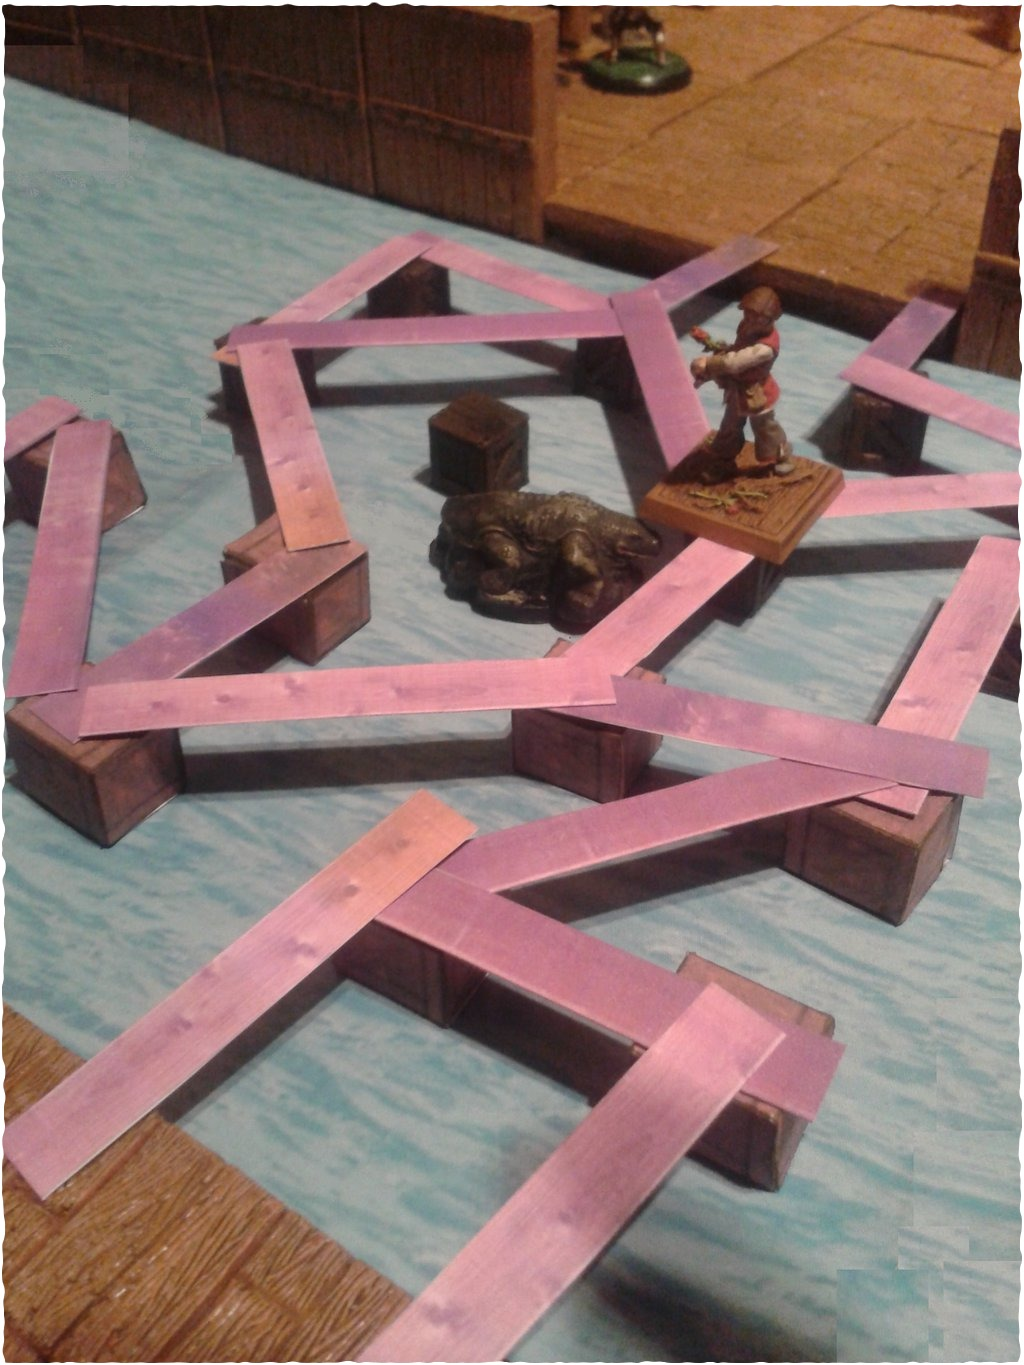
\includegraphics[width=0.4\textwidth]{images/Quint-crossing-the-planks-409036840_mod.jpg}
	\caption{Quint crossing the planks}
	\label{fig:Quint-crossing-the-planks-409036840}
\end{figure}



	%!TEX root = ../crimson_throne_book_main.tex
% 2013-10-26
Wow, that looks nice! Do you have such detailed miniature settings for every encounter?\\



	%!TEX root = ../crimson_throne_book_main.tex
% 2013-10-26
Well, we try to use Dwarven Forge and the compatible Psomminiature scenery with our mini's for the fights. It takes some time to set up, though, and since we're playing at a friend's house, I can't do that in advance, so that factor actually slows us down a bit. I have a pretty nice collection of scenery pieces which are stored in plastic boxes, but that also implies that I have to open maybe five boxes to set up one encounter.I also painted some mini's especially for this campaign last summer, but I don't have a good camera yet to take pictures. Maybe in the future ... These figs are also spread out over several boxes, so while it is great to expand your personal collection of miniatures and scenery, it has one disadvantage: the more material you have, the longer it takes to find what you need. 

	%!TEX root = ../crimson_throne_book_main.tex
% 2013-11-01
The companions go look for the harbormaster and ask him what he knows about {\itshape the Delivery} and its cargo. The man says that the boat carried no goods, apart from food and supplies. Its only cargo was maybe two dozen passengers. The man denies knowing anything about girls being carried off against their wills, but confesses that the authorities can't check everything. The young friends also pay a visit to field marshal Cressida Kroft. They explain to her what happened with Gaedran Lamm, only leaving out that the kept him alive at first and then finished him off anyway before the guards arrived. Kroft confirms that she doesn't like types like Lamm, who live on the edge of legality, and - by paying their vice taxes - are allowed to continue their shady business in the city. She assures the heroes that she will take care of the red tape and make sure that they will not get into trouble for carrying out justice.\\

When the companions tell her that Rolth has left town on a Chelish vessel with a dozen children, she fears that the girls will be sold as slaves in Cheliax. Quint wonders if the skinny creep has made more trips to the south over the last couple of years. Maybe that is why he was so hard to locate, because he wasn't always around.\\

\section{6 Desnus 4708}

The following morning someone knocks on the door of the old fishery. While Sjo is joking that adventure just comes knocking, he is surprised to find the sour-looking magistrate of commerce on his doorstep, Garrick Tann, Korvosa's tax collector, also known as the 'most hated man' in the city. He is accompanied by eight guards and two men wearing the colors of Abadar. The companions immediately recognize the magistrate and also remember that they lifted his purse when they were children, including his masterwork dagger, that now hangs on Puk's belt. Sjo shoves that halfling out of the way, while making polite conversation. Tann states that the companions owe the city ten percent of their income. Having heard that they were given 1 200 gold sails by the queen, he is here to collect 120 GP.\\

When the heroes don't pay him right away, Tann informs them that they have until the end of the month to pay up. They also have to declare any other income they have. They can do so in his office, which is located in the shadow of Citadel Volshyenek. The magistrate also notes that the friends are staying in an abandoned building, which by law should go to the city and can't just be taken over by anyone who feels like it. Still, these matters are not his to handle, although he will inform his colleague.\\

To avoid future embarrassment with another officer of the law, the companions and the four children living with them decide to move to Zellara's house in Lancet Street for now. They also go and pay their taxes, to avoid having Tann track them down again.\\

\section{9 Desnus 4708}

On the ninth of Desnus Mama Mira contacts the companions and invites them over to the orphanage. She wants to talk to them about Sarai and Lauro, the two halfling children they saved from Gaedran Lamm's lambs. She suspects that the children's grandmother is still alive and well, living somewhere outside the city She asks the heroes return the children to their family. Apparently the siblings' father Bono came from the small town of Heavengard. He moved to Korvosa after his wife had died giving birth to Lauro, when Sarai was only three years old. The girl still remembers playing with her old {\itshape nana} under the apple trees. Three years ago Bono passed away himself and orphaned Sarai en Lauro ended up in Lamm's clutches. Since Mama Mira cannot leave her flock in the orphanage, she implores the heroes to take the brother and sister home. Heavengard is a cozy halfling settlement in a fertile valley at the foot of the Willspin Mountains, nestled quietly on the banks of the Jeggare River. Journeying there takes three days.\\



	%!TEX root = ../crimson_throne_book_main.tex
% 2013-11-01
 \section{10-13 Desnus 4708}

The companions follow the Jeggare river for three days until they reach the first fields and orchards of Heavengard. Suddenly they pick up screams and the smell of burning hay. Looking through a four-foot-high hedgerow, they notice three hulking scaly creatures leaning over a young halfling couple. The attackers are kicking a boy, while a girl with a torn dress is screaming her lungs out. Towering over the assailants is a smoking haystack, which was probably set on fire by the lizardman holding a smoldering torch. The two other lizardfolk have a wickedly barbed club in their hands.\\

The heroes intervene and Balian's greatsword chops down a lizardman warrior in one mighty stroke, while Sjo takes down a second enemy. The lone survivor turns and runs.\\

The halfling boy was beaten badly and has lost consciousness, a situation that Sjo's healing powers quickly rectify. The girl, Maisy Booginsfoot,  thanks her saviors profusely and claims that the reptilemen ambushed her and her friend Jacob Merrybrow while they were ... looking for a stray goat. Quint realizes that the halflings were probably fooling around in the hay and smiles.\\

The companions join the young halfling couple to their village. Jacob and Maisy know Sarai's and Lauro's grandmother well. Her name is Mother Grundy, the town' herbalist, although most people have taken to calling her Mother Grumpy since her son and grandchildren left. They are convinced that she will be overjoyed to see her grandkids alive, but they suspect that she doesn't know that her son Bono has passed away, so they advise the visitors to be gentle when breaking this news.\\

Heavengard is nestled in a picturesque valley between rolling hillsides full of fruit trees. The Jeggare River cuts through the heart of the dale and leads the travelers to a dozen low wooden buildings and two stone ones. Although it has been a long time, Sarai remembers the way to her nana's house. The thick, aromatic smell of herbs pervades the air. Sarai approaches the door and notices that it is slightly ajar. Carefully she pushes it open and gazes into the room. Dried herbs hang from the ceiling and a large cauldron bubbles noisily over the fire. An old halfling woman with a few teeth missing looks up, surprised to see strangers on her porch.\\

"Nana?" Sarai whispers, "it's me, Sarai ... and Lauro ... we've come back."\\

"Sarai? Sarai, is that really you?" A broad smile appears on the woman's face as she wipes her hands with her apron and rushes to the halfling children in her door. "Sarai! Lauro! Oh, Cayden Cailean be praised, my grandchildren have returned to me!" Tears roll over the halfling's cheeks as she pulls the children to her breast. "And where is my son, where is Bono?" she sniffs.\\

"Oh, nana, daddy's gone. He died three years ago. A bad man took us and made us work as slaves, but these heroes saved us!" The old herbalist buries her head between the children's shoulders and cries, while a crowd of halflings has gathered outside her house, staring at the wonderful spectacle.\\

A small chubby halfling with elaborate curly hair and rich, purple clothes steps forward. He makes an elegant bow: "Welcome to our humble town, strangers. Allow me to introduce myself, mayor Ossy Applebottom, I'm delighted to make your acquaintance. I believe we owe you our gratitude for saving and returning some of our own. Please, would you do us the honor of joining us tonight for a small celebration as a token of appreciation? I invite you all to my house after sunset."\\

Jacob Merrybrow introduces his saviors to his family and his mother kindly offers the companions a place to stay at their farm.\\

Later that evening the companions join the Merrybrows for the party at the mayor's mansion, one of the two stone building in town and easily the largest structure. Rosebushes climb up the walls to the left and right of the front door and circle around a stone sign above the door that reads 'Theatre' The whole village has gathered inside, in what looks like a small theatre hall, which is very high for halfling standards and offers ample head space for even Sjo. The room explodes in loud applause as the heroes enter the auditorium. Puk is immediately surrounded by a number of girls. Maisy's sister Frida is clearly infatuated with the courageous rogue and the young halfling appreciates the attention.\\

Mayor Ossy Applebottom thanks the saviors again and entertains the crowd with some music. Afterwards he makes his way to the companions and starts chatting cheerfully. It turns out he did a bit of adventuring himself when he was younger, with Simo Sideburn and Addie Lightfoot, two other halflings, but they are retired now. Since then he has grown a bit, Ossy smiles, patting himself on his large belly.\\

The heroes accept Applebottom's invitation to take to the stage themselves. The mayor even joins them in an improvised version of 'the pied piper'. Ossy is clearly over the moon with visitors who appreciate the fine arts of theater, which seems to be his passion.\\

Although the unexpected return of Sarai and Lauro, the spectacular story of their rescue and the wonderful play of 'the pied piper' excites the halflings, the small folk are preoccupied with another matter. The lizardmen's attack on Maisy and Jacob is not an isolated incident, it seems. While the reptiles from the Broken Axe clan have never felt the urge to leave their homeland of the Feverglades before, they did so twice during the last week. Six days ago Ossy Applebottom and his men were attacked by the scaly monsters at the border of the glades and today the lizards made it all the way to Heavengard! Ossy claims that he and his men were gathering wood when a group of Broken Axe warriors attacked them. They barely managed to escape with their lives and both Simo and Addie were gravely wounded.\\

None of the halflings knows a lot about the Feverglades, other than that it is a dangerous and soggy place where they shouldn't venture. They claim that their habit of avoiding the swamps is part of a mutual understanding with the lizardfolk: the halflings don't go there and the lizardfolk don't come here. But now the agreement has been broken, although no one has any idea why the Broken Axe clan suddenly turned aggressive. It's probably in the monsters' nature.\\

Ossy also knows that the peace agreement between Heavengard and the Broken Axe clan dates way back to the days of Harv Mulder. Mulder was a strange dwarf who lived here more than a generation ago ... well, not "here" exactly, but in the swamps. He got on well with the lizardfolk and negotiated the treaty for the halflings. Mulder lived in a mill by the Jeggare River, in a place where the current was much stronger than here in Heavengard. As far as Ossy knows, only two men have ever ventured into the Feverglades, this Mulder dwarf and - three centuries ago - Montlarion Jeggare, the famous explorer who gave his name to the river.\\

Ossy praises his guests' courage and skill in battle once again and asks them if they want to help protect Heavengard from the attacks of the lizardfolk. He does not understand why the reptiles turned hostile, but it is clear they have become a threat. Today's attack proves their evil intent and it will take more than some simple farmers to defend the town.\\

He offers the companions 200 gold sails form his personal fortune to locate the Broken Axe clan and renegotiate the peace treaty. If the lizardfolk can't be swayed, the heroes should explore other options to keep the village safe. If necessary they should chase away the scaly folk. Ossy stresses again that the halflings don't stand a fighting chance against the Broken Axe clan. Fortunately no villager has died yet, but halflings' luck and Cayden Cailean won't protect them forever.\\

It is late when the companions turn in for the night. Sjo, Puk and Balian quickly sink into a deep sleep, but Quint is plagued by nightmares. He is wandering around a huge keep with high walls and oppressing hallways. He feels tiny, but his hands are enormous. His breath surges loudly through his throat and reverberates in his head. Every dark room is empty and it feels like the stone maze is closing in on him, when he suddenly arrives in a huge hall. The room is bare, except for a fireplace to Quint's left. Flames dance around and throw scary shadows on the walls. One of the dark shades floats closer and takes the shape of a skinny, old man with thin gray hair and hollow cheeks. He is dressed in a long nightgown and looks almost like a ghost. Then the man open his eyes, his fiery gaze burning a hole in Quint's heart, as he sighs: "Finally I understand, brother. You have betrayed me."\\



	%!TEX root = ../crimson_throne_book_main.tex
% 2013-11-01
\section{14 Desnus 4708}

The next morning the adventurers prepare to head into the swamps. Mother Grundy makes them some lunch and warns them about the Feverglade mosquitoes. Those annoying insects transfer the feared swamp fever, but with Grundy's {\itshape smelly smear} , a repulsively reeking ointment, they can protect themselves. Grundy also hands the young friends a flask with a strange brown liquid. She calls it  {\itshape poison poison} , a very strong antidote against swamp fever ... just in case. Ossy Applebottom and his men accompany the heroes to the border of the glades, further down the Jeggare River. Ossy can't give them further instructions: since none of the halflings ever venture into the swamp, no one knows where the Broken Axe clan lives. He sends the companions off with a hearty farewell and reconfirms his hopes for a peaceful solution.\\

The swamp is initially less dirty than the travelers suspected. The Feverglades are not as stagnant as other swamps. The Jeggare River flows through its center and provides the entire area with plenty of fresh water. Fortunately today's water level is quite low, which will facilitate trekking through the marshes.\\

Still, not all corners of the swamp are equally accessible and after a few hours the paths become fewer and narrower. There are indeed a lot of mosquitoes, just as mother Grundy predicted, but the smelly smear keeps the pests away.\\

Suddenly the path gives way to stepping stones across a stretch of water. The big stones have been carefully placed to allow a creature with a stride similar to a human to cross. The surface of the stones shows the occasional scratch, which Balian believes were made by lizardmen feet. He also notices that the stones are sticking out more than one foot above the surface of the water and the brown and withered moss on their sides suggest that the water level used to be higher.\\

While making his way across the stones, Quint loses balance and tumbles into the filthy muck, where he is immediately attacked by an alligator. Balian jumps in next to him and cuts open the creature's leathery skin, but the ranger sees his friends missing their attacks and is violently snapped into the alligator's maw. Unable to wrestle from the sharp teeth, Balian is pulled under water as the swamp killer performs its feared death roll. He loses consciousness as his friends further attempts to harm the alligator or put it to sleep with magic fail horribly. The ranger is barely clinging to life when Sjo, who has joined him in the filth, sends some healing through him and finally kills the predator with a lucky swing of his burning morningstar. It takes four charges from the healing wand to return Balian to health.\\



	%!TEX root = ../crimson_throne_book_main.tex
% 2013-11-02
Again a snapshot from our session:\hyperref[fig:Swamp-encounter-410834455]{ swamp encounter } . \\

\begin{figure}[h]
	\centering
	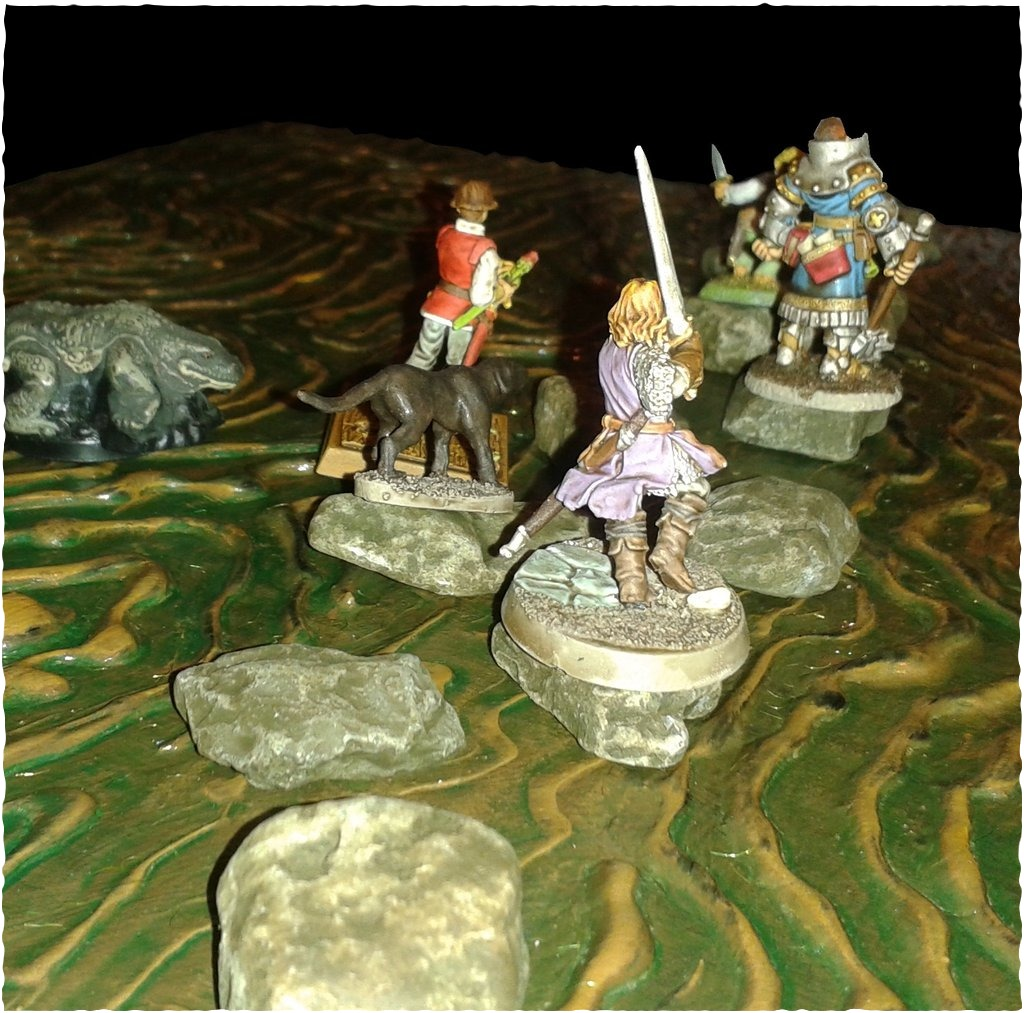
\includegraphics[width=0.4\textwidth]{images/Swamp-encounter-410834455_mod.jpg}
	\caption{Swamp encounter}
	\label{fig:Swamp-encounter-410834455}
\end{figure}



	%!TEX root = ../crimson_throne_book_main.tex
% 2013-11-02
 The picture looks really nice. I think you're getting your money's worth with that alligator miniature, so far. :)\\



	%!TEX root = ../crimson_throne_book_main.tex
% 2013-11-16
The companions resume their trek across the stepping stones. Past the crossing they see a small cluster of huts, made of wood and woven bulrushes. Wooden racks sport fresh fish drying in the sparse sunlight. Several lizardfolk with spears and clubs await the visitors around some kind of shrine in the center of the village: four standing axes arranged in a circle with their heads touching. Necklaces and personal items hang from these rusted weapons.\\

There are about two dozen lizardfolk present, including the women and children. Although they seem suspicious, they do not attack the strangers entering their village. One of the males slips into the water behind the huts and swims away in the direction of a small hillock, some 200 yards to the north. A single blackened tree stump sits on top of the mound.\\

Another lizardman with broad shoulders and a wicked club on his belt raises his hand as a peace sign. He also grumbles something in draconic to his fellow clan members in an effort to calm them down and keep them from attacking. Although he cannot speak common, he uses gestures to invite the visitors over to a wooden raft. When they have boarded, he slips into the water and pushes the primitive boat over to the hillock with the tree stump.\\

As the heroes climb the mound, they notice that the stump is hollow and hides the entrance to a dark cave. Below they hear the sound of something moving in the water, followed by a hissing voice: {\itshape Sssss, I don't know whether to welcome you or curssssse you, ssstrangersss. You come here from that clan of falsssse little folk, I sssssee you even bring one of them to my home ... ssssss. We've never had any quarrel with them, that issss until resssssently. Two moonssss ago they entered our territory and they have been draining our ssswamp ever sssssinsssss.}  Firsssst we waited for them to ssssstop, then we tried talking to them, but they killed our negossssiatorssss. Then we ssssent our warriorssss to the wheelhoussssse, but they were defeated.\\

Sssso a couple of dayssss ago I ssssent sssscoutssss to the little folk'ssss village. Although they alssso met with violensssse, I do believe that you are the anssswer to my sssscoutssss' pressssensssse. We are not looking for a war, sssso I will give you the opportunity to sssay your piessssse, but do not missstake thisss kindnesss for weaknessss, for if we have to, we will kill every one of thossssse ssssmallfolk, ssssss.\\



	%!TEX root = ../crimson_throne_book_main.tex
% 2013-11-16
I like the way this adventure is built, it gives a tough choice to the players... Very nice.\\



	%!TEX root = ../crimson_throne_book_main.tex
% 2013-11-17
The final discussion on whether Ossy Applebottom has actually done anything illegal or not, actually lasted for about an hour and a half. I just wrote down the gist of it.At one point I even burst out laughing, remembering similar sessions when we had captured enemies alive and discussed at length what to do with them before someone finally got tired of it and simply bashed in the prisoners' heads. Still, Applebottom's chances look slightly better and I actually believe he might survive. 

	%!TEX root = ../crimson_throne_book_main.tex
% 2013-11-24
\section{15 Desnus 4708}

The companions spend the night in the mayor's manor, while keeping the Ozzy and his two minions locked up in the cellar. When mornings comes, all the halfling villagers gather at the house. They are not pleased when they find out Ossy Applebottom is behind the problems with the lizardfolk and that he tried to fool all of them for his personal gain.\\

Quint suggests that someone else assumes the position of mayor and appoints mother Grundy. His inspiring speech gets all the villagers to agree. Then he explains that he and his friends will take Ozzy over to the Broken Axe lizardfolk in order to negotiate a permanent solution.\\

While they are making their way through the swamp again, Sjo and Quint intimidate the former halfling mayor with horror stories of cruel lizardmen rituals. Ozzy offers the heroes more money, simply for letting him go, but they refuse. When they arrive at the Broken Axe settlement, they are taken to the island with the tree stump again, only this time they can enter the cave through an opening in the back of the hillock.\\

The leader of the clan turns out to be a glistening water naga, who goes by the name of Naamani. She is furious when she learns that Ozzy thinks himself the owner of swamp land, but when she squeezes him between her coils, the halfling readily agrees to sign all marshland over to the water naga and her tribe. The lizardfolk reward the companions for their good work by giving them a beautiful pearl.\\

Next stop is the watermill. The dwarves and gnomes are still at work, draining the glades, when the companions arrive. Quint states that the swamp has a different owner now, who has ordered the trespassers to stop their work and leave the Feverglades. He adds that Ozzy will pay them what is owed upon arrival in Heavengard. Gilas, the gnome engineer, realizes that he has no other option than to agree. So the dwarves and gnomes join the young heroes for Heavengard, but only after they have buried the lizardfolk heads. Gilas also confirms that the water level in the glades will return to normal in a few months time. The engineer shuts down the draining system and Quint and Balian sabotage the pumps, so no one can restart them by simply pulling a lever.\\

It is late in the afternoon when the party gets back to Heavengard. The locals have not been idle either: they have decided to strip the three traitors of all goods and banish them. One of their own, the village merchant Rollo, will travel to Korvosa tomorrow with three carts of goods. He will take Ozzy and his men and release them in Korvosa.\\

Mother Grundy also rewards the party. Since the halflings have no desire to gain from Ozzy's banishment, they have decided to award Ozzy's confiscated ring and Simo's armor to the heroes. Using Zellara's harrow deck, Sjo finds out that both items are magically enhanced: the gold band is a ring of {\itshape protection +1} , which goes to Balian, while the small sized  {\itshape studded leather +1} fits nicely around Puk's chest. The party halfling also enjoys his last evening in Heavengard. The village youngster admire him as their personal hero and red-cheeked Frida is even more infatuated with him than before. Puk does not return to his bed that night.\\

\section{Level up: level 2}



	%!TEX root = ../crimson_throne_book_main.tex
% 2013-11-24
\section{16-18 Desnus 4708}

The heroes return to Korvosa in the company of a small convoy. Merchant Rollo and his two sons ride on wagons and each carry one of the culprits. Simo and Addie prove to be no threat and are quickly relieved of their bonds. Even Ozzy is not tied up anymore on the second day of travel. He realizes that his scheme failed and he's lucky to have gotten away with his life.\\

After three days of travel Korvosa finally graces the horizon. While approaching their home city, the companions note that several small plumes of smoke rise up and a great number of travelers has been stopped at the gate, creating quite a queue. When they join the line, Quint learns that the king has died a couple of days ago. The city has been in chaos ever since. All non-natives are being denied entry to the city, so the four young friends have to say goodbye to their fellow travelers, as they are the only ones who are allowed in.\\

The companions quickly make their way to the High Bridge. Houses in East Shore have all shut their doors and shutters and there are only a few people in the streets. The ones who are, rush to their destinations as quickly as they can and keep their heads down. Someone has chalked a message on the wall of an old building: ``No whore for queen!''\\

When they reach the High Bridge into the city proper, Quint, Sjo and Puk question some guards to find out what is going on in Korvosa. They learn that the king died on the thirteenth of Desnus. Unable to regain his health, Eodred was finally felled by his mysterious disease. None of his doctors or priests managed to find a cure. Riots erupted shortly after the monarch's death as people protested against his incapable, power-hungry widow Queen Ileosa assuming the throne. No one actually knows if the queen has what it takes to take over power, but the general consensus seems to be that Ileosa is nothing more than the "sois belle et tais-toi" (shut up and look nice) type, not fit to rule. There is even more worrying news, as seneschal Neolandus Kalepopolis has disappeared shortly after the king's death. He is rumored to have died in the first riots.\\

Eodred's Walk, the square at the far end of the High Bridge, has been overrun by rioters. Several hundred protesters are pushing back Korvosan Guards in the direction of Citadel Volshyenek, the Guard's headquarters, shouting hateful words like: "Hang the b+\$~\#!" or "Down with the filthy usurper!" The demonstrators charge the soldiers and one of the guards loses his balance while his brothers in arms are trying to retreat. The crowd cheers and gets ready to tear the man to pieces.\\

Quint jumps in their midst and attempts to sway the attackers with words. He urges them to calm down and use common sense. He points to Korvosa's historical strength in unity. Both Puk and Quint recognize some dockworkers in the crowd whom they address in person. "Dorik, don't risk your life, your mother needs you!" "Gerrit, your wife's pregnant, don't do anything stupid!" Sjo throws in some religious motives: this riot goes against Abadar's need for structure, it undermines civilization. Quint also picks out the most hot-headed protestors and focuses his attention on them. Meanwhile Sjo and Balian pick up the unfortunate guard and return him to the safety of his brothers' ranks.\\

Quint's and Sjo's words persuade enough people in the crowd to step down and soon the mob disperses and the threat is averted. The last to leave are a number of head-strong troublemakers who look like the main agitators. But they also leave when they see that they have lost the crowd's support.\\

The companions join the guards to the citadel, where they meet up with Field Marshal Cressida Kroft. The leader of the guard looks tired, as she confesses to not having slept for a couple of days. Sjo offers to help and Kroft gladly takes him up on his offer.\\

She explains that a number of guards have failed to show up for duty. Although everyone was ordered to come in and serve, several soldiers refused, worrying more about their family's safety than the city's. While Cressida Kroft does not condone, she can understand why these guards have 'deserted'. Still she needs every able-bodied guard to be at his post right now. Moreover, this kind of behavior is bad for the morale of those who are present.\\

Yet, not all deserters have family. Some of them are simply using the riots as an excuse for personal gain. One such man is Verik Vancaskerin. Upon the king's death, he convinced several fellow guards of the queen's incompetence and together they deserted their posts. They have now set up shop in an old butcher's, All the World's Meat, in Northgate, handing out free meat to citizens in need, while spreading messages of hatred against Ileosa. Kroft does not dare to send in her own men to apprehend the deserters, fearing their talk of secession might infect even more guards. She also dislikes the idea of guards killing fellow soldiers. So she asks the companions to take care of the situation. She prefers the traitors alive, certainly Vancaskerin himself, as she wants to find out why he deserted.\\

After a quick stop in Zellara's house, where the remaining lambs are all safe, the companions head to the North Point district. As darkness is already upon them, they decide that it is not a good idea to go to the butcher's shop right now. Still, they use the first few nightly hours to gather some information on the place. The word is that a couple of guards have taken over the place and hand out free meat every morning. The deserters have taken to calling themselves the Cow Hammer Boys and rumor has it that you can hire them to get rid of small pests. Apparently they took care of Dicey Dewy, a local rogue, two nights ago. The thug has not been spotted since.\\

Someone else admits to having been inside the butcher's. A note on the wall says: "We provide what the queen can't", referring to the fact that most shops have been closed for the last four days and food has been getting scarce. There are four cow Hammer Boys: Baldrago, Malder, Parns and Karralo, all able-bodied and battle-hardened soldiers. Their boss, Vancaskerin, does not show his face very often. People say that he still wears his uniform. The companions decide to leave things for now. They will return in the morning and see if they can approach the deserters "peacefully".\\



	%!TEX root = ../crimson_throne_book_main.tex
% 2013-11-28
Oh, wow, they are only level 2... It seems that they have achieved so much already! (probably because of the introduction, when they were kids)\\

I liked the side-treck in Heavenguard. I was wondering:\\

 

	%!TEX root = ../crimson_throne_book_main.tex
% 2013-11-28
 

	%!TEX root = ../crimson_throne_book_main.tex
% 2013-11-29
Makes sense. :)\\



	%!TEX root = ../crimson_throne_book_main.tex
% 2013-12-07
\section{19 Desnus 4708}

Today marks the day that King Eodred II will be buried, but apparently it will not be a public event. So there is no way the companions will be able to witness the funeral, especially since - as Quint explains - the royal crypts are underneath the castle. Moreover, the king's burial will be a private ceremony within the castle walls, as the queen does not want to risk inviting more trouble in the city streets.\\

So the young friends are free to pursue their own little plot in North Point, where the butcher's shop known as {\itshape All the World's Meat} will be handing out free meat again to the unfortunate citizens who are finding it increasingly difficult to get food elsewhere. Quint suggests taking a diplomatic approach and after some deliberation the heroes decide to pose as sympathizers to the anti-queen movement. When they arrive in Stirge Street they find the butcher's shop overrun by dozens of people. Only a few customers fit into the shop itself, so most clients crowd the street in front of the building. Balian inspects the house and finds out that the front door is not the only way inside. A cattle pen is built against the left side of the building and since it is open to the air, Puk can stand on Sjo's shoulders to sneak a peek over the wooden fence. He notices a side door leading into the back of the house. Still, this early hour is not fit for a covert operation, so the companions decide to take a frontal approach.\\

Sjo joins the crowd waiting outside the shop and start pushing everybody into a line to create some order. While everyone is reluctant to queue at first, it quickly becomes obvious that this orderly manner of waiting is much more enjoyable for all those present. Meanwhile Quint sweet-talks his way into the building, by claiming he only wants to talk to the men inside and is not interested in getting free meat. When the bystanders see his expensive attire, they believe him and allow him to cut in line. Two men are behind the counter in the cramped shop, where customers are standing elbow to elbow. Quint recognizes the man with the bushy unibrow and flat nose from the descriptions they got last night as Baldrago. He introduces himself as a sympathizer to the cause and agrees on returning in a few hours, when today's meat has run out and there are no more customers.\\

The companions continue maintaining order outside and Quint entertains the crowd with a bit of music and jokes about the queen and her Gray Maiden lovers. By noon Baldrago and his mate send home the remaining people waiting outside, as there is no more meat to hand out. There are only a few pieces left in the shop window, covered in flies, but those will stay there until the sun sets, so they urge the unfortunates who have to leave empty-handed, to try again then. Next they invite the companions inside. A short conversation reveals that the four men working for Verik Vancaskerin, the so-called Cow Hammer Boys, are not all that interested in sabotaging the queen. They certainly do not seem to be hard-line political activists. But maybe their boss is. Quint and his friends are allowed to go upstairs to talk to the man in charge.\\

The companions arrive in a room with a round table and some bedrolls on the floor. A clean-shaven man dressed in Korvosan livery and armor walks in and greets them. Although he seems to be slightly more politically motivated than his mates, he still does not come across as a hardliner at all. He seems to be more interested in keeping the poor people fed than in feeding them hatred against the queen. He is mostly worried what will happen when his shop runs out of animals to slaughter. Quint wonders if Verik had any support setting up this shop, but the former sergeant of the Guard gets vague at this point. He admits to having friends who arranged his little set-up, but claims not to be able to contact them himself. He also refuses to spill any more information on this as he says it is a private matter. Sjo hints at Quint not to press the subject and next it is Verik Vancaskerin's turn to ask the companions some questions. He informs about their motives and plans. When they claim they want to support the cause in a way similar to Vancaskerin, he agrees to let his 'employers' know when the contact him, although he has no clue when that will be.\\



	%!TEX root = ../crimson_throne_book_main.tex
% 2013-12-07
The young friends return to Citadel Volshyenek. On their way over there, they pass a mad prophet on a street corner who has gathered some unlookers. The wild-haired old man preaches that " {\itshape the eye of Groetus has turned from the Boneyard of Pharasma to look upon Korvosa} ", claiming that "  {\itshape Korvosa's darkest hour is still to come! It will spell doom for all! Time to make peace with your loved ones, before it's too late!} " Sjo and Quint's witty remarks that they are already at peace with everyone and that if there will ever be an end of days, it is inherently drawing closer every day, makes the raving lunatic lost for words. When the companions arrive in the Citadel, they come across some soldiers practicing in the courtyard. One of them, a woman in a helmet, faces a tall, cocky man, who taps his sword on his shield while joking: " {\itshape So, you all expect me to hit a woman? Save yourself the trouble, honey, lay down and allow me to plunge my sword into your body.} " The woman suffers this jests undauntedly and return the favor: "  {\itshape From what I hear that sword of yours is not much more than a butter knife, Barvos. Come to mama, then we'll see who really has the balls in the family!} " The male guard dislikes being made fun of himself and leaps forward, lunging wildly at his female colleague, who deftly steps out of his reach and kicks him in the behind as he surges past her. The man returns more cautiously now, trying to force back the woman with more measured strikes. She catches each one of them with her sword or shield. The mere sound of the blows suggests that the man is putting a lot of his strength in them. Then the woman takes the offensive: she is quicker and more precise and now the man has to give way to her. When frustration takes over, he wildly bashes his shield against hers, putting all his body weight into the punch. His attack throws back the female guard a couple of feet and breaks her advancement. The two adversaries now start circling each other, using more predictable tactics trying to hit one another. After a few minutes the female guard seems to be getting tired, as her shield sags a few inches. Her opponent seizes the opportunity and leaps at her, but her tiredness was just a ruse. She dives under his sword and hooks her blade behind his foot, tripping him. As the male guard bites the dust, the woman kicks his weapon from his grip: " {\itshape Those balls of yours need to grow some more, Barvos} ", she jokes. Then the woman notices the companions. She removes her helmet to reveal a sea of lush red hair. As she faces the young heroes, they recognize her as Amarice, their former fellow lamb. She is madly enthusiastic about seeing her old friends and greets them warmly with big hugs and a broad smile of joy. Since she is still working at the moment, she agrees to meet the companions later this evening at the Travelling Man in Old Korvosa.\\

In Kroft's office the young heroes fill in the field marshal on Verik Vancaskerin's new operation. They explain that they discovered little political motivation in Verik and his men and wonder if anyone is forcing him to cooperate. Cressida clarifies that Verik is unmarried and has no ties in the city, since he immigrated here from Riddleport. So she does not believe that someone is threatening his loved ones to make him do something against his will, as he doesn't seem to have close relationships in town. There are hundreds of soldiers in the guard who would make much better targets for such a scheme than Vancaskerin. Sjo suspects they will have to search for whoever is 'sponsoring' Vancaskerin in Korvosa's higher circles, but cannot provide a ready answer to the question what drove the sergeant to quit his post.\\

Upon hearing that Vancaskerin is more worried about getting food to the people than spreading lies about the queen, the field marshal stresses once more that the companions have to do their best to take him alive, as her deserted sergeant might not be a bad man as such, just misguided. Still, his treason is a glowing ember of rebellion among other soldiers who contemplate quitting the Guard for personal reasons, most of them to protect their families. So the deserters have to be taken care of as soon as possible. The normal punishment for desertion in times of military need is death. Kroft says she is prepared to look at Verik's case personally to see if he merits a less severe punishment, but he will have to be punished one way or another. She also advises the companions to transport Verik and his men to the Longacre Building if they are taken alive. Longacre houses the city's courthouse and prison, and it is much closer to Vancaskerin's new headquarters than the Guard's Citadel.\\



	%!TEX root = ../crimson_throne_book_main.tex
% 2013-12-07
After their visit to Cressida Kroft, the companions return to the north of the city, to Old Korvosa, where they hang around in the local pubs looking for more signs of trouble in the city. They learn that the {\itshape Ironsooters} , the men and women who work in the Ironworks, are on strike. They protest against the fact that Korvosa bans guilds. The mastersmith, Baris Trenchlow, has always been in favor of guilds and seizes this time of civil unrest to voice his opinion. When evening arrives the young friends join Amarice in the Travelling Man. Their former lamb 'sister' is eager to learn what happened to them over the last four years. She also tells them that she joined the Guard almost immediately after they freed everyone, since she always dreamed of being a soldier and felt she would be safe from Lamm in the guards' ranks. She spent a few months in the Citadel's kitchens, but flirting with some of the soldiers sufficed to get her in the recruitment program. She has been a Korvosan guard for three years now. She has not stayed in touch with other former lambs, though.\\

She also enquired among her colleagues in the Citadel about Verik Vancaskerin and learned that he has a new girlfriend who has started seeing some three months ago. She does not know the girl's name, but rumor has it Verik is crazy about her.\\

After a lovely evening the companions return to {\itshape All the World's Meat} . They stake out the place for some time, until they see the four Cow Hammer boys leave. Puk follows the four deserters while his three friends make for the butcher's shop. Balian gets out his thieves' tools and picks the lock on the front door. The three companions quickly head upstairs and surprise Verik Vancaskerin in his private room. Verik is seated at his desk, carving the table with a dagger in his left fist while staring at a letter in his other hand. When the intruders reveal that they are here to arrest him, Vancaskerin draws his longsword and waits for them to attack. "  {\itshape Traitors sent by the queen} ", he hisses as he dodges under Balian greatsword and resists Quint's  {\itshape sleep} spell. He swings at Balian with both his longsword and dagger. The ranger avoid the long blade, but is cut by the sidearm. Then Sjo hits the sergeant hard with his burning morningstar. Quint's second attempt at  {\itshape sleep} is successful (finally!) and prematurely ends the fight. Balian and Sjo tie up the sleeping sergeant while Quint casts a  {\itshape detect magic} , discovering that Vancaskerin's cloak and dagger are magical. Then the bard examines the letter on the desk:\\

 {\itshape Dearest Verik}  Stirge Street 22 houses an abandoned butcher's shop. The former owner died in prison, where he rotted away for not paying his taxes. The building itself has been in the city's custody since then, awaiting to be sold to cover the tax debt. You undoubtedly are familiar with our government's inefficiency, so it won't surprise you that the shop stood empty for more than a year.\\

Behind the boarded windows you'll find a decent place of business. If you reopen it, you can do more good for Korvosa's citizens than by playing sergeant and suppressing the good people of our city. A dear friend of mine wants to help the common man, but requires assistance from someone trustworthy. I know no one I trust more than you, my love. My friend will supply a number of animals for slaughter, so you can distribute their meat for free to the man in the street. For the common man will be the first victim of this incompetent harpy on the throne. We can't allow for our fellow citizens to starve to death, so we'll just have to provide what the queen can't.\\

I love you to pieces and I'm eternally yours ...\\

S\\



	%!TEX root = ../crimson_throne_book_main.tex
% 2013-12-08
PUK, CG Male Halfling rogue (swashbuckler) 2                 Fast-Talker  Personal Addiction ---\\

QUINTILIAN CG Male Human bard (court bard) 2                    Trained actor  Fast-Talker  Child of the Street \section{Satire}

---\\

BALIAN CG male Human ranger 2 (urban ranger)               Trained actor  Child of the Streets  Reactionary ---\\

SHAOBAN, LN Male Human oracle 2           Abilities Str 14, Dex 10, Con 12, Int 8, Wis 14, Cha 18   Clouded Vision  Flame Mysteries  Touch of Flame  Trained actor  Child of the Streets  Ease of Faith ---\\

Spyder, N dog companion level 2            

	%!TEX root = ../crimson_throne_book_main.tex
% 2013-12-23
Just a quick note... as someone who is running this campaign (twice!), I really appreciate the amount of detail and effort you've put into this journal... it really brings the story alive and makes for a great read!\\

Many Thanks to you and your players :)\\

Tim\\



	%!TEX root = ../crimson_throne_book_main.tex
% 2013-12-26
Thanks for the kind words. I hope you' re having fun as well, even the second time around.\\



	%!TEX root = ../crimson_throne_book_main.tex
% 2013-12-26
It's actually very different... one group is halfway into Part 3 (7 players!) and the other is halfway through Part 2 (4 players) Looking forward to your groups further adventures!\\

Kind Regards\\

Tim\\



	%!TEX root = ../crimson_throne_book_main.tex
% 2013-12-30
The young heroes transport Verik Vancaskerin to Citadel Volshyenek. This time at night the streets are mostly clear of people, so they reach their destination without any trouble. Field marshal Cressida Kroft is still awake, although she looks tired. She is just saying goodbye to another guest, a priestess of Sarenrae. Sjo recognizes the woman as Sadira from his days in the temple of the sun goddess.\\

The companions quickly brief Kroft on how they arrested sergeant Vancaskerin and hand her the letter they found on his desk. She has Verik locked up in the dungeons and Sjo and Quint enter his cell to interrogate him. Verik claims that he's been doing more good for the people in Korvosa by handing out free meat than he ever could have done as a sergeant in the guard. The price of bread has tripled in the last couple of days and the poorer citizens simply can't afford to pay for their food. The riots in the city have also caused numerous businesses in town to temporarily close their doors, so a lot of families are without income at the moment. Vancaskerin also believes that his good deeds in {\itshape All the Worlds Meat} probably created more order in that corner of the city than the entire Guard did. Sjo doesn't care about the man's motives, saying that nothing excuses breaking his vow to the Korvosan Guard. A word is a word! When Quint steers the conversation in a political direction, Vancaskerin freely admits that he has no love for the queen, seeing her as an incompetent little girl who only cares about her own beauty and luxury. If she is allowed to take the reigns over the city now, people will regret it later on. It's better to act sooner rather than later and have her removed from office now, before she can dig her nicely manicured claws into the position. Quint mocks the sergeant's na\"ivet\'e, as he doesn't even seem to know who he is working for. Verik replies that he'd rather have someone in charge who feeds the people than someone who lets them starve. The queen has never shown any interest in the people of Korvosa in the past five years and her failure to get a grip on the situation now, only proves her incompetence.\\

When asked about his girlfriend, Verik admits that she is of Vudran descent and that her name is Selena. He met her only two months ago and has been seeing her irregularly. Apparently he doesn't even know where she lives or how he can get in touch with her. But she knows how to find him and when she does, they seem to share the same ideas on life and politics. They have been sharing their concerns on the queen's incompetence to rule since the king got ill and when Verik received her letter to help to poor people of Korvosa five days ago, he immediately rose to the occasion. Since then he has been waiting for Selena to drop by, eager to show her the good job he did with the butcher's shop. Unfortunately, she hasn't shown up yet. Quint is just flabbergasted by the sergeant's short-sightedness. He can't see he is being manipulated and he has no ideas who is really pulling the strings. He doesn't want queen Ileosa to sit on the throne, but he cannot present an alternative ruler.\\

Before they leave the man to rot in his cell, Quint and Sjo want to know more about Vancaskerin's allies, the four other deserters. Verik doesn't really know them that well, other than that they had a reputation for being pig-headed. They were known for giving their officers a hard time and trying to avoid getting the harder or more dangerous jobs. When Verik overheard them complaining about having to risk their lives in the riots to protect that stupid, self-loving little b\&\#\\



	%!TEX root = ../crimson_throne_book_main.tex
% 2014-01-04
Wow, I love the rooms you've built for the miniatures. That seems to really add a great deal of visual immersion to the gaming experience. Does it take a long time to set these things up?\\

Are you able to re-use a lot of the same walls, furniture, etc, without it getting too visually repetitive?\\



	%!TEX root = ../crimson_throne_book_main.tex
% 2014-01-05
These set-ups were done outside of the game session. We play at a friend's house, because I live far away from everyone else, so my scenery stuff is usually in his apartment, but I brought it home for the holidays to test out my new camera.During play we only set up the areas where combat takes place, to allow for the strategic movement. It takes a fair few minutes during play to set up a scene, more so since I've been expending my collection and now I need to browse through more boxes to gather the pieces I need. I've been reorganizing a bit to try and improve this situation in the future, but since I do not play at home, I cannot set up scenery in advance, so that is a pity. Setting up these larger sceneries requires even more time, especially when you add the time to take pictures and rebuild things to make a second floor or something. Still, the fact that I have all this wonderful material urged me to try something like this for once. I also photographed some scenes that are still to come, so I'll be adding more pictures in the future. Get ready to see my version of the Marbledome opera house, the Shingle chase or the courthouse from As far as the repetitive issue is concerned, I've never been bothered by that, even when I had less material. During our previous campaign our DM used print-outs of the battlegrounds, but in my opinion nothing compares to the modular 3D options of Dwarven Forge and Psomminiature pieces. 

	%!TEX root = ../crimson_throne_book_main.tex
% 2014-01-11
The companions continue their search in the dock area to find the mysterious rabble-rousing Vudran beauty, Selena. The anti-queen sentiments flow strong in the northern ward of the Midland district. Although the Korvosan Guard still patrols this area, the soldiers seem self-conscious and wary.\\

Suddenly two shadows sweep over the young friends, as two Sable Company marines fly over on their hippogriffs. A third rider is falling behind: his flying mount is bleeding from several wounds and struggles to remain in the air. The black-armored pilot cannot keep his animal airborne any longer and crashes around the corner, immediately followed by a crowd of angry dockworkers: "Over there! He went down! Get him!" Puk promptly sets off in pursuit, followed by the others. The halfling surprises one of the hot-headed rioters in the back, while Quint weaves his bardic magic to put another troublemaker to sleep. Balian's greatsword cleaves down another two, so the remaining hooligans quickly abandon their efforts to kill the soldier - whose leg is trapped under his wounded mount - and flee the scene.\\

Sjo pulls the marine from under his hippogriff and heals both the man and riding animal. The soldier is grateful and recognizes Sjo from his days at the Great Tower, the headquarters of the Sable Company. He warns him to be careful in this neighborhood, as things are getting more out of hand every day. After another well deserved 'thank you' he leaves for his home base.\\

The information gathering trail finally leads to the {\itshape Bailer's Retreat} , a rough tavern that is actually pretty close to the companions' home at Zellara's shop. This place is normally frequented by a high number of Korvosan Guards who like the strong coffee, but rumors say that soldiers avoid the spot at the moment. The young investigators decide to don a disguise before continuing their hunt for Selena. Quint dresses up as a dockworker, Balian takes off his armor and reconnects with his simple oarsman outfit. Sjo ties a strip of cloth over his eyes and hides his big frame in a dirty cloak, assuming the guise of a blind beggar. Puk trusts his ability to keep to the shadows and remain from sight, allowing him to track his friends and step in when necessary. At the {\itshape Bailor's Retreat} Quint finds no clues to Selena, but he does learn the name of another rabble-rouser, a man named Birold who frequents  {\itshape The Bountiful Mermaid} , an alehouse in West Dock. A witness who dislikes the riots attests to having seen the man inspire hatred for the queen and government in others. Quint decides to give the watering hole a quick look-over, but at this nightly hour there are only drunks left at the bar and Birold is not among them, although - when served with a drink - one of the patrons states he will most likely be in tomorrow evening. 

	%!TEX root = ../crimson_throne_book_main.tex
% 2014-01-11
\section{22 Desnus 4708}

The first order of the day is getting a new {\itshape wand of cure light wounds} , as the current one is almost depleted. Sjo knows that the best place to find such an item is the temple of Sarenrae. On the steps of the Sun Goddess's church two parties are locked in a violent discussion with a priest. A couple of soldiers are carrying an unconscious colleague on a stretcher. Facing them is a tear-faced mother and her wounded 12-year-old son. The boy is clinging his left arm closely to his body, trying to prevent his broken bones from hurting too much. "In the name of the law, I demand you see to my man!" the sergeant of the Korvosan Guard commands.\\

"But my son, he's so young ... he's hurting so much, the poor thing can hardly breathe. Please heal him, we're devote followers of Sarenrae", the woman sobs.\\

"Young, you say? He was old enough to cause a riot and throw stones at my men! If you heal him instead of my soldier, I'll arrest the lot of you for disturbing the queen's peace!" the sergeant bellows as his hand slides towards the hilt of his blade.\\

Seeing how hard pressed the priest is, Sjo steps in. "There is no need for a fight. There is enough healing to go around, don't fret." Nathan, the priest, recognizes the former acolyte of Sarenrae and his face lights up. Sjo gauges the situation and quickly establishes that the boy's wounds need to be treated sooner than the soldier's. If the broken arm is not set right, it won't heal properly and leave the kid handicapped for the rest of his life. The soldier might have lost consciousness, but his wounds are not severe. He urges the priest to heal the boy, while he tends to the soldier with a {\itshape cure light wounds} of his own. Balian is the only one who sees through the weeping mother's deceit. Although she claims to be a true follower of Sarenrae, she sports a medallion of Asmodeus around her neck. Still, Sarenrae's priests are the only ones who hand out healing for free, so she has come to the home of the Sun Goddess instead. Nathan still helps her by giving her son his last cure spell of the day and hopes that this charity will make her see Sarenrae's value.\\

When the guards, the mother and son have left, Nathan invites the companions in. He is really pleased to see Sjo. Although he still doesn't quite understand where the big man gets his divine powers from, he figures it has something to do with his Shoanti heritage, giving him a shaman's skills rather than a priest's. Even so, he claims that this mystifying source of Sjo's powers should not prevent him from praying to Sarenrae. He also explains that he and his fellow priests have been very busy helping the wounded. As Sarenrae is the only church in town that heals people for free, the clergy has been hard pressed by requests for medical aid. As the priests only hand out their daily allotment of spells free of charge, they usually go through their curing arsenal pretty swiftly. Most people who are turned down because there is no more healing left, return early the next morning, which leaves most priests depleted of healing magic by the time the sun has properly risen. That also explains why he had only one cure spell left for the two wounded parties. Nathan takes his guests to see Iris, who handles the commercial transactions. She happily sells Sjo a fully charged {\itshape wand of cure light wounds} . Quint and Sjo also wonder what the queen is up to. Since she hasn't really shown her presence over the last couple of days and she hasn't made any decisions to solve the chaotic situation, they fear there might be trouble. Quint would like to procure an audience with the monarch to offer his help, but doesn't know how to proceed to get in to the castle to see her. So he decides to write a letter to the captain of her bodyguard, Sabina Merrin. In it he explains what he and his friends have done and learned over the last few days and offers his services to the city and the crown, urging her to contact him. He hands the letter to one of the Gray Maidens who are guarding the palace. He also notices a strong presence of Hellknights in the streets surrounding the castle, which explains why this area is so quiet.\\

Sjo suggests paying a visit to the Gray District, since he would like to find out what happened to the seneschal. Neolandus Kalepopolis disappeared during the first hours of unrest, but nobody seems to have a clue what happened to the man. Sjo questions the priests of Pharasma to find out whether the seneschal's corpse might have been brought in and buried. Keppira d'Bear assures him that she has not seen Kalepopolis' body among the victims of the riots. She knows the seneschal in person and unless his cadaver was so badly damaged that it was unrecognizable, she is sure he was not buried with the nameless deceased.\\

Sjo also establishes that the Shoanti are still here. Gaekhen explains that their diplomatic mission has not changed, but the visitors from the Cinderlands are waiting for a more opportune time to approach the queen. Since the feud between his people and Korvosa is buried in three centuries of blood and hatred, it would not be wise to be too hasty. The conflict is three hundred years old, a few more weeks won't matter. Sjo also questions Thousand Bones about his take on the riots and the presence of the castle on top of the mastaba. The old shaman does not understand the situation. Although the Shoanti know both leadership by family ties and leadership by strength, all parties involved are always open and upfront about their intentions. The people of Korvosa act incoherently and no strong leaders have presented themselves and taken control. As far as the castle is concerned, he regrets this insult to his people, as the mastaba is a holy place for Shoanti, but he realizes that he has to accept this fact if he wants to negotiate with the city's leaders.\\



	%!TEX root = ../crimson_throne_book_main.tex
% 2014-01-11
That evening the companions get into their disguises again and head to {\itshape The Bountiful Mermaid} . Tonight they are lucky, as one of the patrons is Birold. The good-looking dockworker is in the middle of a game of darts. The target is a roughly-hewn likeliness of the queen, on which the more deadly areas have been painted red and yellow, granting more points when they are hit with a dart. Birold wins the game of  {\itshape death to the whore} and treats his comrades to a drink afterwards, toasting to a quick downfall of the queen. Quint joins them and introduces himself as a dockworker from Old Korvosa. He challenges the winner of the previous game to a new round of darts and comes out the victor, leaving him to pay for the next round of drinks. He notices that Birold does not finish his mugs so as not to get intoxicated. During their conversation Birold spills that something is going down tonight and that he will have more to offer supporters of the just cause tomorrow. If Quint is interested, he should probably come back then. At half past eleven Birold leaves. Puk stealthily follows him, with the others hanging back even more . The dockworker makes for a warehouse, where he is joined by four more laborers. By midnight a dashy fellow arrives in the company of two bodyguards. While the man slips through the doors, the guards take up position outside and watch the area. Curious to know what is going on inside, the companions decide to act. Quint manages to take out the two guards with a successful sleep spell, giving Puk and Balian the opportunity to sneak into the depot. There are plenty of crates where they can hide and listen in on the conspirators, who have gathered in the back of the building.\\

The dashing man is addressing the dockworkers: "Friends, the whore still hasn't understood. She continues wallowing in the luxury that our sweat provided. We have to raise our voices even louder. Tomorrow we'll organize another march against the usurper. Gather as many sympathizers as you can and bring them to the Gold Market and Eodred's Walk. There we will issue our complaints once more. The market and its stores will be the regrettable target of our actions, as grievances are only heard when it hurts! The power of merchants in the city will serve as our coin in this confrontation.\\

Just like in the demonstration against Citadel Volshyenek you will be joined by others, hailing from all over the city. Once more I have to stress the importance of keeping our destination a secret until the last moment. We don't want the Guard to be in the loop.\\

We also feel that civilians have to be well informed on what is going on. That is why our men infiltrated the university of Korvosa last night and started the presses to print a special number of the Korvosa Herald, the Korvosa Rascal. I've brought a few hundred copies for you to hand out among your friends.\\

I also fear that we'll be opposed again, by both the Guard and the Hellknights. It is too bad that these bucket-heads can't see what is really going on, they are so blind in their obedience. But when they face us with sharp steel in their grasp, we cannot afford to stand empty-handed. I've brought clubs that you can distribute among your strongest supporters. Here!"\\

At that the man pulls the sails off a cart, revealing numerous weapons inside. "Don't get me wrong, friends. I abhor violence, but if that is the only language they understand, we have to be prepared. Remember, comrades, if your mighty voice erupts, all of Korvosa stops! Death to the Chelish whore! For a free Korvosa!"\\

The dockworkers join in as they gather around to get their copies of the Korvosa Rascal and the clubs. By this time Quint also sneaks into the building, but when Sjo follows him, one of the men inside hears something and notices that the front doors are open. "Feldon, why aren't the doors closed?" he asks the dashing gentleman. This is the companions' clue to spring to action.\\

Quint overtakes one of the dockworkers with another successful sleep spell. Balian and Sjo attack from the right and knock down one of the conspirators. Birold is the first to counter; he draws his mace and smashes it down hard on Spyder's back. Balian reacts furiously and cuts heavily through the man's chest, but Birold is tough and remains afoot for now. Quint has less success on the left side, as he gets hit twice by a club. The dockworkers might not wear any kind of armor, but their muscled arms can dish out some serious damage. The bard tries to hold the left flank, aided by Puk's stinging short swords, but both of them get wounded seriously while taking down an opponent. Feldon, the dashing gentleman, mumbles the words of a spell and blinds Sjo, Balian, Spyder and Birold with a splash of golden particles. He joins the fray and thrusts his flashing rapier twice between Balian's ribs, badly wounding the ranger. Still, the two blinded friends quickly regain their sight and take out one more enemy.\\

Quint manages to disarm another adversary and Puk can finally take him out. When Feldon sees that most of his supporters have been defeated, he decides to run for it. He catches Balian and Sjo in a spot of slippery {\itshape grease} , dropping them both to the floor, as he makes for the door. While the ranger and healer drag themselves out of the greasy area and overpower the final dockworker, Quint uses his last spell to stop Feldon. For the third time tonight he mutters his incantation and for the third time in a row the magic hits home. Feldon stumbles to the ground and lays down his head, slipping away in the warm embrace of slumber. 

	%!TEX root = ../crimson_throne_book_main.tex
% 2014-01-12
Nice, I like the way you're really fleshing out the rioters.\\



	%!TEX root = ../crimson_throne_book_main.tex
% 2014-01-15
I'm really liking this journal and all the work you've put into fleshing out Korvosa. You're making me want to start up a second Crimson Throne campaign to flesh out the city as much as you have. If only I had the time :(\\



	%!TEX root = ../crimson_throne_book_main.tex
% 2014-01-19
Having followed one of the rebellious dockworkers to a secret meeting in a warehouse, the young heroes have discovered that someone is actually instigating the riots. A brief but tough fight left most of the rabble-rousers unconscious, although Puk's vicious blades made one casualty that cannot be saved. The main instigator, a dashing bard by the name of Feldon, failed to get away when Quint's {\itshape sleep} spell took him down. The companions tie him up and decide to interrogate him before they call in the guard. At first Feldon seems fervent in his belief that the queen is incompetent. Her lack to take control over the last few hectic days only proves this point. Quint wants to know who Feldon is working for, but although the man is quite chatty, he is also extremely vague. He lets on that he might be more willing to cooperate if his captors provide him with an outlook on a future. To say it plainly, if he's handed over to the guard, his fate will be sealed. He wants a way out. It takes two broken knees (apparently this is turning into Sjo's trademark interrogation technique) before the squirming prisoner can convince the companions that he will only speak if they guarantee not to hand him over to the guard. If the heroes give him their word - especially Sjo, who clearly demonstrates his faith in the law and in 'a word given' - he is willing to stay in their custody until the problems in the city quiet down. He's even prepared to give his own word not to try and escape during this time, if he'll be allowed to go free afterwards. In exchange he can provide valuable information or so he claims. After some deliberation the heroes agree.\\

Then Feldon confesses: he is working for someone who has no political agenda at all. His employer only has his own economic interests at heart. By destabilizing Korvosan society his boss hopes to plummet real estate prices, so he can buy up huge portions of the city and acquire a position of note in Korvosa. Feldon's help in this scheme is equally inspired by greed as the bard is handsomely paid for his services. With some luck he might even be able to copy his employer's plans on a smaller scale and invest in some Korvosan houses or businesses. The man Feldon works for does not hail from Korvosa, but from Cheliax: he's the Chelaxian ambassador Amprei!\\

While most of the dockworkers are still unconscious from the fight, one of them was defeated with a {\itshape sleep} spell, just like Feldon. This man was tied up and awoke shortly after the battle, before the companions started interrogating their prisoner. He has heard every word the honey-voiced bard has confessed to, and now he fumes with anger. Quint and Sjo use some charges of the  {\itshape cure} wand to bring the man's fallen comrades back to consciousness and when they all realize they have been played by a money-grubbing Chelaxian dandy, they are equally enraged. Now they understand that they have been risking their lives so someone else could get rich off their blood. Instead of wanting to march against the queen and convince others to join them, they now want to stop as many Korvosans as possible from rioting for a misguided cause. This insight more or less turned them from misled enemies of the state into defenders of the peace, so the companions decide to let the men go, as they are now bent on preventing tomorrow's demonstration. Feldon is taken to the old fishery and locked up in Gaedran Lamm's old room. He explains that the Vudran beauty Selena is someone like him, who was inspiring another cell of instigators elsewhere in the city. Those people will have the same agenda as the one Feldon was trying to give to the dockworkers. Tomorrow at noon, they will gather their supporters and head for the Gold Market for a violent demonstration. Balian remains behind to guard the prisoner while his friends make for Citadel Volshyenek to inform Field Marshal Kroft of the impending uproar in the city's commercial center.\\

Cressida Kroft is asleep behind her desk when Sjo, Quint and Puk arrive. She is shocked to learn that ambassador Amprei has been feeding the riots for his personal gain, but she immediately states that it is impossible for anyone but the queen to act openly against the Chelaxian emissary. She will have to consult with some people to see what can be done about the man. Until that time the companions should not take action against Amprei. Still, priority has to go to tomorrow's demonstration. Kroft will inform her officers and work out a plan to prevent the manifestation. It looks like another night without sleep for her ...\\

\section{23 Desnus 4708}

When the companions wake up the next morning, they feel well rested and even more equipped to tackle today's challenges (level up to level 3). When to head to the market they find it completely locked off by the Korvosan Guard. Anyone trying to get in is turned down and sent away. Quint and his friends join some men who have come from the Shingles and return home after the guards refused to let them pass. A fellow called Evald, who normally hangs around in {\itshape The Blue Drake} , told them that today would mark a turnaround in Korvosan history as the people would demand to be heard in a massive manifestation in the Gold Market. Apparently someone snitched on these plans to the guard, as the soldiers were not supposed to be in the loop. More disappointed marchers have gathered in the Blue Drake, but there is no sign of Evald. The innkeeper knows where he lives, though, in a flat two blocks away. Quint leads his friends there, but finds only a young frustrated woman, who is annoyed that her husband is out rioting again. She has no idea where Evald is and actually gets worried when she hears that he is 'missing'.\\

Back in the Blue Drake Quint inquires about Selena. The innkeeper confirms that Evald has met with a Vudran lady a couple of times, although he doesn't know her name. She was quite a looker, though. A few hours later Evald shows up in his favorite haunt. Quint gets to talking with him, informing him that people in the docks are telling strange tales: the riots are apparently caused by someone who wants to throw the city into chaos to undermine the real estate market and buy up huge portions of the city. Tales about the queen's incompetence were fabricated to fuel an evil scheme of a power-hungry villain, who was using Korvosan citizens as propellant. He also adds that a woman named Selena is one of the evildoer's agents. Evald is shaken; as the news sinks in, he gets furious at having been deceived, a sentiment that is quickly shared by other patrons in the tavern.\\

Seeing that their rumor spreading is so successful, Quint and his companions spend the rest of the day in the Shingles, feeding the gossip channels, dissuading more people from supporting the anti-queen movement. They make sure to mention the Vudran snake in the grass, Selena, as an accomplice of the unknown manipulator. After all, she's not the only one who can sway minds with words.\\



	%!TEX root = ../crimson_throne_book_main.tex
% 2014-01-26
\section{24 Desnus 4708}

This morning Sjo makes some time for the three remaining ex-lambs: Mouse, Korwick and Heldrin. He gives them some basic weapon practice and tests their ability for the divine and arcane arts, discovering that Heldrin shows some spiritual talent. Meanwhile Balian trains his dog Spyder and Quint goes into the city to gather more information on ambassador Amprei. He locates the man's impressive villa in South Shore. He already knew that Amprei frequented the gambling ship {\itshape Twin Tigers} in Eel's End, but now he learns that the ambassador also likes to visit the  {\itshape House of Clouds} , the brothel ship. In the evening Quint, Sjo and Puk head for the brothel in Eel's End, hoping to find out more about the Chelish nobleman. It's a hard job, but someone has to do it ... Sjo disappears with ginger-haired Danarella in one of the rooms, while Quint visits with his favorite Vudran girl, Yuuna, and Puk meets the cute halfling Reena. The rogue is so overwhelmed by this new experience that he forgets to ask about the ambassador, but Sjo and Quint pick up that the Chelaxian prefers the twin sisters Lani and Leni.\\

Later in the evening the three friends pay Lani a drink. When they inform about the ambassador, she lets on that he is a client, but she is reluctant to share what happens between the sheets. Quint's smooth talking finally gets her to admit that Amprei never sleeps with her and her sister at the same time, but always with just one of them. During his climax he addresses them as "Vera", as if the girls remind him of someone by that name. Quint wonders if there is a link with Verana Ornelos, a noble born girl from House Ornelos (she is Lord Toff's grand niece).\\

Since the {\itshape Twin Tigers} gambling den is another of Amprei's favorite haunts, the three friends stop over there as well. Quint joins a game, and while winning some money, he learns that the Chelish ambassador occasionally enters the private quarters of Eel's End's big boss, Devargo Barvasi. When the heroes enquire if they can meet with the 'spider king', they are told to return the next day in the afternoon, when Barvasi will be interviewing candidates to join the enforcers that guard his docks. 

	%!TEX root = ../crimson_throne_book_main.tex
% 2014-01-26
\section{25 Desnus 4708}

In the afternoon Puk, Sjo and Quint return to Eel's End. They are allowed into Devargo Barvasi's cabin, which has been converted into a throne room of sorts. The walls are covered in webs which hold dozens of spiders, some as big as a man's fist. Two sturdy oaken tables with chairs flank the door and seat half a dozen burly blokes. On the other side of the room a wooden stage supports a large throne; in it rests a tall man in black leather armor with steel spider-shaped ornaments. His legs are casually slung over the right arm of his seat while he's petting a hairy spider on his chest. He smiles lazily at his guests and invites them to take a seat. Sjo also notices the desperate look in the eyes of a tiny purple dragon in an iron birdcage hanging from the ceiling next to the throne.\\

Quint immediately cuts to the chase and says they are not here to join the enforcers, but rather to talk to the spider king. Barvasi reacts by remarking how tall Sjo is and invites the Shoanti to entertain him with a small game of {\itshape knivesies} , a pirate tug-of-war from Riddleport. Knivesies has two contestants standing opposite each other on a wooden table. Their right hands are bound together with a wet leather strap and they have an empty belt pouch strapped to their belts. Fifteen gold sails are put on the table between them, as is one dagger. The person who ends up with most coins in his purse wins. Sjo is bound to one of the enforcer candidates and figures he has the best chance in an honest fight without weapons. Being the first to act, he tries to kick the dagger off the table, but it has been planted in the wood firmer than he expected and the big Shoanti only manages to partly dislodge it, thus providing his opponent with the opportunity to pull the small weapon out of the table. Still Sjo feels confident that his armor will protect him and decides to make a show of it, sending jolt after jolt of flaming fire through his hand until his opponent drops to his knees. The poor man only managed to nick him once with the slightest of cuts. Sjo recovers the knife, cuts through the leather strap and stabilizes his adversary before reaching for the gold and placing the sails into his pouch, one by one. When his purse is full he tosses it at Devargo Barvasi, who smiles contentedly. The King of Spiders weighs the pouch in his hand and then gives it back to Sjo: winner's keeper's! Next he sends out the candidates, giving his three other guests a private audience first.\\

Quint impresses his host by recognizing his Riddleport accent and by pointing out that the big spiders are much more harmless than the small brownish specimen in the webs behind him. The poison of that 'recluse spider', or 'violin spider' as it is also called, can lead to skin necrosis. Fortunately these spiders are rarely aggressive, unless provoked.\\

Barvasi appreciates Quint's little display of knowledge and asks him why he is here. The bard tells him that he tried to contact him before, in vain that time, to talk about Rolth, a drug brewer. As he senses that the spider king dislikes the man Quint continues by saying that he has now left the city and is out of the picture for the moment. Today however he has a different agenda: he would like to know more about the troublesome ambassador Amprei. Devargo replies that he's met the Chelaxian a few times in person and - as he feels the companions bear the foppish nobleman no love - he lets on that he has some power over the man that he'd be willing to sell to his guests, for the right price, of course.\\

Sjo offers him 500 gold and Devargo claps his hands in delight: "I love the way the world works, you invest 15 gold in a game of knives and get 500 in return, marvelous!" He asks his visitors to wait while he goes below. When he returns he's holding two letters which he hands to Quint. Both sheets bear a whiff of perfume and contain an overtly sexual message from someone called Verania Tvastiox addressed to her secret love Amprei. Quint knows her as the wife of Agmanar Thrune, a mighty conjuror and cousin to Her Infernal Majestrix, Queen Abrogail II of the Thrice-Damned House of Thrune in Cheliax. If the ambassador has been sleeping around with this powerful man's wife, evidence to the fact would surely destroy him. Barvasi admits to having stolen the letters from the ambassador and selling them back to him at the rate of one every few weeks. By paying 500 gold sails the companions have just secured the last two copies in Barvasi's possession. The spider king bids his guests good luck with their new acquisition and says goodbye.\\

Realizing that these compromising letters give them a real hold over Amprei, the companions hurry to citadel Volshyenek, where they report their findings to the Field Marshal. Cressida Kroft is very pleased, and while the scandalous nature of the letters sends a blush of red to her cheeks, she states that they should work perfectly as leverage against the cursed Chelaxian. She will contact the castle and make arrangements for the companions to be received there tomorrow at ten o'clock. She is also very grateful for the fact that the heroes' actions with the rioters have had such great results, as order is slowly returning to the city. Yesterday and today have been the first two relatively quiet days since the king died. She repays her agents the 500 gold sails they spent procuring the letters and hands them another 500 gold as a reward.\\



	%!TEX root = ../crimson_throne_book_main.tex
% 2014-01-26
BALIAN, CG Male Human ranger 3 (urban ranger)                 Favored Community Korvosa (Ex)  Favored Enemy (Humanoid (Human)) (Ex)  Trapfinding (Ex) Trained actor  Child of the Streets  Reactionary Spyder, dog companion level 3, N Small animal           ---\\

PUK, CG Male Halfling rogue 3 (swashbuckler)        {\itshape silver short sword +2} +9 (1d4+2/19-20) and  {\itshape masterwork short sword} +8 (1d4/19-20)         \section{Sneak Attack (Ex)}

Fast-Talker  Personal Addiction ---\\

Quintilian, CG Male Human bard 3 (court bard)        {\itshape rapier +1} +5 (1d6+3/18-20)             Bardic Performance  Versatile Performance (Comedy) (Ex)  Countersong (Su)  Distraction (Su) You can use your performance to counter magic effects that depend on sight.  Heraldic Expertise (Ex)  Satire  Mockery (Su) Trained actor  Fast-Talker  Child of the Street ---\\

SHAOBAN, LN Male Human oracle 3               Clouded Vision  Flame Mysteries  Touch of Flame (Su)   Molten Skin (Ex) Trained actor  Child of the Streets  Ease of Faith 

	%!TEX root = ../crimson_throne_book_main.tex
% 2014-02-01
\section{26 Desnus 4708}

The next morning the companions finally get their second audience at Castle Korvosa they have been hoping for. Before they leave they wonder what they should talk about with the queen. Opening up the gates so trade can resume and food can get back into the city is definitely a priority. Quint also wants the Hellknights out of the city, as those narrow-minded fools cause more problems than they solve. As far as increasing the popularity of the queen is concerned, 'bread and games' are a sound concept. Maybe there should be some kind of official coronation with festivities.\\

A knock at the door pulls the young friends out of their brainstorm. A Korvosan guard is waiting outside. The shape of the soldier's armor betrays that she is of the female sex. As she takes off her helmet, the heroes immediately recognize Amarice, the woman who was in Lamm's lambs with them when they were children.\\

"Good morning," she says, 'I'm here to officially remind you of your appointment with the queen at ten o'clock. Meeting her majesty ... that's a great honor! You've been doing a fabulous job for our city, I've been told. Preventing riots, arresting deserters and what not? You even helped out my dear colleague Grau when he was down. I guess the city and the queen owe your their gratitude. Not bad for three little lambs ... I see Lamm's cruel upbringing didn't spoil your true hearts, it even strengthened them." Amarice looks a bit self-conscious before continuing: "Anyway, enough with the big words, I also sought you out to ask for a personal favor. You remember when we were kids and we witnessed King Eodred showing off his new bride to Korvosa. The Field Marshal presented Ileosa with her own private guard, the Gray Maidens. We were only a few yards away, as you recall. Well, ever since then it has been my dream to serve her majesty as one of her Maidens. I wonder if you'd be willing to put in a good word for me ... please." Amarice holds her head slightly slanted and bats her long eyelashes. "For old times' sake ..." Sjo is open to Amarice's request, but tells her that they have more urgent matters to discuss with her majesty, so he can't make any promises. Still, he'll see what he can do.\\

At the castle the companions walk in on a familiar scene: in the entrance hall they meet the impatient and nagging man in impeccable clothes again, ambassador Amprei. He looks as haughty as ever and immediately starts ranting as the company comes in: "By all the gods, good and evil, what is wrong with this stupid, boorish dump? You maggots are here again while I'm wearing a hole through the floor, being made to wait like ...uch ... a servant? An outrage!"\\

At the same moment Sabina Merrin steps in and interferes: "You'll be right up, mister ambassador ... thanks to these heroes no less. Enjoy the peace and quiet, while you can!" Then she welcomes the companions and escorts them to the throne room. Seated on the crimson chair of power is Ileosa, dressed in black. The only ornament she is wearing is her father's brooch. Despite her sober outfit she still looks gorgeous. Field Marshal Cressida Kroft is already in there with the queen.\\

"Your majesty," she bows, " these are the heroes I've been telling you about." Quint kneels and his friends quickly follow his example. Ileosa lifts her black veil as her sweet voice resounds through the great hall: "Noble heroes of Korvosa, you have my thanks ... again", the queen smiles radiantly. "This time you do not only prove a favor to me, but to the entire city of Korvosa. If I'm to believe the Field Marshal, you singlehandedly prevented a bloody manifestation and took out several agitators who were plotting against me. But worst of all is this low-life Amprei who thinks that he can turn my own people against me! The traitor! Fortunately you've provided me with the prefect weapon to get him out without burning our bridges to Cheliax." Ileosa's hands shake as she holds up the two compromising letters from Verania Tvastiox.\\

"But first things first. I would like to reward you for your services to the city." Ileosa rises and approaches the companions. Sabina Merrin steps forward as well, presenting a small box to the queen. Ileosa opens the lid and takes something from inside. "Quintilian of Korvosa, Sjo the great, Balian the bold and Puk of the small-folk, for services provided to the city of Korvosa I hereby proclaim you honorary members of the Order of the Pseudodragons." She hangs a medal around each of the four men's necks. The gleaming medallion portrays a tiny dragon in flight.\\

"And now we must see to more pressing matters, the unfortunate case of ambassador Amprei. I would like you to bear witness to the fruit of your good deeds, although I must ask you not to interrupt. This is between Amprei and me!"\\

Sabina Merrin leaves the hall and returns a few moments later with the Chelish ambassador. "Your majesty! Finally I get to see you! You won't believe how long I've had to wait. Truly, a disgrace! I've been waiting here from well before your husband passed away ... for which I offer my condolences, by the way. But now to more urgent matters ..."\\

"Indeed, there are other matters we need to discuss!" the Queen bellows. "Time for each of us to learn their rightful place!"\\

"And that starts on your knees, KNEEL!" Sabina Merrin hisses as she forces the surprised Chelaxian to the ground.\\

"Your Highness! Now you can witness firsthand what I have to go through in this hellhole. You come from beautiful Cheliax, just as I do. These primitives don't know the meaning of the word {\itshape manners} ", Amprei grunts as he tries to rise, but Sabina Merrin clutches his shoulder and keeps him down. "Primitives, you say?" I see only one primitive here, even though the term sounds too kind for you. A worm, a conniving lowlife ... that is what you are!" Ileosa spits out.\\

"But, your majesty, please, I do not understand ..."\\

"What is it that you don't understand? That I'm on to you and your cowardly plans? Do you take me for a fool? Because I'm a woman, perhaps? Do you deny your ambitions to buy up buildings and lands in this 'hellhole', as you so condescendingly call it?" the queen rages.\\

"What do you mean? I've never bought anything here, except for my villa ..." Amprei stammers.\\

"Of course you haven't bought anything yet! Everything is still too expensive. Allow chaos and disorder to run wild in the streets a little while longer ... and then our little ambassador will open his wallet to save the poor citizens by purchasing their properties for next to nothing. Why would you buy today what you can get for half the price tomorrow? Oh, don't get me started on the likes of you!" Ileosa counters.\\

"Ileosa Arvanxi, I have to warn you, when her Infernal Majestrix learns of how you're treating me ..." the ambassador attempts, while he slips from Merrin's hold and rises to his feet.\\

"I think her Infernal Majestrix would rather know how you are treating her cousin's wife, Verania Tvastiox," the queen retorts, "who likes to please you with every hole of her body!" Ileosa pulls out the two letters the companions gave her and stares down Amprei, who pales and is left lost for words.\\

"Oh no, what's this? Don't know what to say anymore? You can count your blessing that you are here as the official ambassador to Cheliax, or I'd have you quartered and beheaded for such an offence! Here's what you are going to do, Darvayne Gios Amprei! You're going to resign your post and get the hell out of this city forthwith! Let's call it {\itshape health issues} , because if you stay for even one more day, your health will most certainly be at risk! Even this far-away hellhole won't protect you from the ire of Agmanar Thrune when he gets a hold of his wife's letters! And that piece of property you already own here in Korvosa, you'll sign it over ... well to Korvosans who truly deserve it, these brave heroes!" Ileosa gestures. Amprei is shaking in his shoes while the companions are dumbstruck by this sudden turn of events. The Chelaxian throws the heroes a venomous glance and turns around. Then he walks out without speaking another word.\\

"That takes care of business", the queen smiles as she straightens her dress and reclaims her throne. "As far as you are concerned, my loyal citizens, I could use your help again. The unsettling first week of my rule as queen of Korvosa has not been a success. Time for mourning the king is over, however. It is time I prove to Korvosa once and for all that I'm capable of ruling her and that I can restore order. In two days time I'm calling the great council to the palace. I would like for the four of you to be present as well, so you can report on what you've witnessed in the streets. I don't have to remind you that we cannot discuss the Chelish ambassador, as we do not want to lose our hold over him by exposing his dirty laundry. But you can inform the council of all the other things you've discovered. Furthermore, I'd appreciate any ideas you have to offer to improve the image of the Korvosan government in general and my person in particular. Can I count on you?"\\

"It will be our pleasure, your majesty", Quint replies.\\

"Then I will see you in two days. We'll convene at eight in the evening. And you, Field Marshal Kroft, are expected as well"; the queen concludes.\\

"I'll be there, your majesty", Kroft replies. She bows and signals for the companions to follow her out.\\

As they step into the open air again, Cressida beams with pride: "Congratulations! You've made quite an impression on the queen, Order of the Pseudodragons, a villa in the finest district of the city and an invitation to the council, alongside the high and mighty of Korvosa. Not bad, not bad at all."\\

Back in Zellara's parlor the companions examine their medallions. The amulets carry magic that slightly hardens their wearers' skin, making them harder to hit. A precious gift.\\

In the evening Quint and Sjo spread the word in various inns and alehouses that the great council will gather in two days. Apparently the government is getting ready to take control again. They also find out that the common people of Korvosa are mostly interested in getting fed and feeling safe. Others also add that they would like to get back to work. Quint will make sure to mention this at the council.\\

\section{27 Desnus 4708}

Two Gray Maiden show up at our friends' place to guide them to their new home, Amprei's villa. Sjo tells the three kids, Mouse, Heldrin and Korwick, to remain in Zellara's shop while he and his friends go and check out the new place. The kids are very disappointed, but their sad faces and teary eyes cannot convince the Shoanti to let them come.\\

While walking to South Shore, Balian suddenly gets a broad smile across his face, but his mates cannot get him to tell them why he's smiling. When they arrive on the villa's doorstep, the urban ranger grins again, as he signals the three kids closer who have been following them secretly. The children are beaming with enthusiasm as the double doors open and the magnificent edifice lays before them. The Gray Maidens hand Quint the deed to the place and take their leave.\\

The building looks mostly intact, as Amprei only got time to pack his personal items. His clothes and papers are missing, but all the furniture is still in place. The villa also includes a large walled garden and a coach house with stables. There are no horses anymore, but there still is dashing carriage. The companions are overwhelmed by the beauty and luxury of their new home, but decide to get settled in nonetheless. They spend the rest of the day moving in their meager possessions and waiting for a locksmith to replace the lock on the front doors.\\



	%!TEX root = ../crimson_throne_book_main.tex
% 2014-02-01
\section{28 Desnus 4708}

Now that they have a classy home in South Shore the companions realize that their clothes have to match their abode, especially since they'll be meeting with the leaders of the city later that day. So they spend most of the day buying a new attire and having their outfits fitted to perfection.\\

At eight in the evening they make their way to the palace again and meet the bigwigs of Korvosa, who have all gathered in the throne room. Cressida Kroft waves the heroes over as they enter and introduces them to Commander Marcus Endrin of the Sable Company, Lord Mercival Jeggare, one of the richest men in the city, and Lord Valdur Bromathan IV, who has broken with his family's tradition of military service in favor of a career as a priest of Sarenrae.\\

Also present is Archbanker Darb Tuttle of the bank of Abadar, the city's most powerful priest, who is locked in conversation with two magistrates, Syl Gar, the Magistrate of Expenditures, and his 'counterpart' Garrick Tann, the Magistrate of Commerce. While Syl Gar is responsible for spending levied taxes on the city's behalf and is thus greatly loved all over, Garrick Tann is the chief tax collector, who is often referred to as {\itshape the most hated man} in Korvosa. The companions met this man before and already dread their next encounter, as they will have to pay a ton of taxes for the various magical items they have recently acquired and for their new home. Another familiar face is that of Zenobia Zenderholm, the high judge. She is talking to another noblewoman, Eliasia Leroung, the head of the university of Korvosa who responsible for printing the Korvosa Herald. The third person in their company is a handsome man with a clever look in his eyes, Glorio Arkona, the only nobleman who lives in Old Korvosa, where he is considered somewhat of a hero by the poor, for whom he provides cheap housing.\\

There is one more person in the room, a sour-faced old man with a long white beard and purple robes. He is seated all alone by the hearth. Quint recognizes Lord Toff Ornelos, the headmaster of the Acadamae and possibly Korvosa's most powerful arcanist. The bard greets the loner and kindly inquires about the Breaching Festival, the annual competition in which students and a number of invitees attempt to break into the Acadamae and breach its many magical defenses. Tomorrow is the 29th of Desnus, on which this festival normally takes place, but Quint has picked up rumors that the holiday will be cancelled this year. Lord Ornelos confirms the news, groaning that it wouldn't be proper to celebrate while people are killing each other in the streets.\\

Next Sabina Merrin, the commander of the Gray Maidens, steps into the room. "Ladies, and gentlemen, I give you ... the queen!" The leaders of the noble families bow, while the two magistrates and the four young heroes get to their knees. Queen Ileosa walks in, as glorious as ever. She is no longer dressed in black, but strides forward in a flowing green silk gown which is once again complimented with her father's brooch. She glides over to the throne and takes a seat, allowing herself a few breaths to let her eyes wander over her guests. When she speaks her voice is calm but strong: "Ladies Zenderholm and Leroung, my lords Jeggare, Bromathan, Arkona and Ornelos, Commander Endrin, Field Marshal Kroft, Archbanker Tuttle, Magistrates Tann and Gar, sirs Quintillian, Sjo, Balian and Puk, I bid you all a warm welcome."\\

The guests are all ears as Ileosa continues: "I have convened the council to discuss the state of things in Korvosa, and for this occasion I have asked a few advisors to join us. Would you all please follow me to the royal reception room so we can commence healing our wounded city?"\\



	%!TEX root = ../crimson_throne_book_main.tex
% 2014-02-01
The queen leads those present to the next room, where she sits down at the head of a long table. The nobles take up position close to her majesty, leaving the companions and the magistrates the places at the other end of the table.\\

When everyone has settled, Ileosa speaks again: "Ever since my husband died the city has been sinking away in chaos: riots, destruction, pillaging, battles with the Guard or other representatives of the state, numerous wounded and too many dead ... all in the name of a queen who cannot rule! This has to stop, right NOW! That is the reason why we have all gathered here today.\\

The Sable Company and the Korvosan Guard have been working night and day to prevent us from slipping away completely into the Abyss. I was even forced to call in the help of the Hellknights to enforce order. But disorder overwhelmed us nonetheless.\\

We may count ourselves lucky that we have creative citizens like these heroes and sharp minds like Field Marshal Kroft. Their firm actions saved us from even worse. Field Marshal Kroft, would you please fill us in on what has been going on in the city?"\\

Cressida Kroft rises and addresses the members of the council: "I understand that our citizens were shocked by the King's death. Eodred was a good ruler and the people loved him. But why did they react so vehemently? I had a hard time understanding that. Grief was normal, but all this anger, hatred and rebellion were out of place. That is why I sent out these gentlemen, to find out what was going on. I'll let them fill you in on what they discovered."\\

Next Quint takes the stage: "When our good king died, it felt like there was a sudden void in power. We have to respect that his widow needed time to bury her spouse and properly grieve him, but some people seemed bent on not allowing her that time. Individuals who had some personal reason to criticize the government, who had their own agenda. They took disadvantage of the moment, swaying the minds of other Korvosan, honest, hard-working citizens who unfortunately don't exactly grasp how politics work. One thing led to another and the situation got out of hand, fast. The city reacted promptly to these challenges, but while actions like closing the gates probably saved innocent lives, it also provided these enemies of the state with more fuel for their fires of rebellion, as food supplies quickly dwindled away and the people grew hungry and malcontent."\\

"I appreciate your report, good master Quintillian," Glorio Arkona interferes, "but you're not telling us anything we don't know yet. Can you give us something more concrete?"\\

"I can. We walked in on a manifestation that almost got out of hand. If we hadn't convinced the misled protesters that killing guards would only make matters worse, the day would have ended in blood. This was the first time we felt that most people were just following some agitators who spewed filth on our beloved queen. We found more evidence to this theory when we stopped a business called {\itshape All the World's Meat} . A clever agitator had duped a lovesick guard and some of his unworthy colleagues into handing out free meat to the poor. The leader didn't even realize it, but his men were actually killing people and carving up their flesh to feed the citizens. We also saved a member of the Sable Company from being torn to pieces by agitated dockworkers and witnessed a troop of Hellknights slaughter a dozen people who had been dumb enough to follow a handful of rabble-rousers into manifesting against the queen. We weren't able to save them all, but I don't even want to imagine the bloodbath that would have taken place if we hadn't been there. We came across honest citizens who were so brainwashed that they almost tore captain Jalento's young son to pieces or who were so hungry that they threatened to kill a baker for food. Finally we were able to track some of the agitators. We shut down their little operation and with the help of the Guard, we were able to prevent another march that was meant to end in violence and blood. Since then we have been using the same weapons as our enemies, a silver tongue, spreading the word on their treasonous, self-serving manipulations and convincing the good people of Korvosa to give queen Ileosa a chance.\\

After all, when you talk to the average John Doe, you quickly find out that all he wants is to be fed and to feel safe. You have all noticed it, but the last couple of days have been more or less quiet again. We have turned the momentum of the enemies of the state, now we have to press on!"\\

"And when you talk about {\itshape enemies of the state} , do you know who they are?" Archbanker Darb Tuttle of Abadar wonders. "I'm afraid not", Sjo replies. "We have been fighting and rooting out the symptoms rather than the cause. But we have been successful nonetheless. Our priority has always been the safety of the people, so that has been our terrain of operation, the common man in the streets. Even an invisible enemy can be beaten if we take away his weapons and prevent his evil schemes."\\

Eliasia Leroung adds: "What these young men are saying is true indeed. There have been people at work who want to taint the queen's reputation. Just a few days ago our presses were abused by such rabble-rousers to print a fake edition of the Herald with all kinds of filth about her majesty. I learned that these heroes intercepted about half of those papers, but several hundred copies were still distributed. You might have seen them. Even when we don't know who is behind these evil plans, we should act! I will make sure that the next edition of the Herald rectifies the situation and reveals the fact that rabble-rousers have been at work."\\

The council readily agrees with this proposal, as Leroung continues: "My family also holds a stake in many of the city's docks. Our laborers have to get back to work, there might be a dozen grain ships waiting in the bay to be unloaded. Getting people back to work and bringing food into the city is the best way to get things back to normal. There's no business than business as usual."\\

Garrick Tann, the tax collector, supports this proposition, as it would allow him to resume his work as well. "People were attacking soldiers in the streets, even without me there. I couldn't risk causing even more of a stir by doing my job. Still, part of these missed taxes will never be recovered. Getting the city back to running will cost money. I propose that those who can afford it, help us out. I think the noble houses should make an extra contribution, lest we go bankrupt."\\

It is clear why Tann is so unpopular, as about half the people at the table raise their eyebrows in surprise and annoyance at his proposal. Glorio Arkona keeps his bearings and replies: "I'd be willing to contribute a little extra, lord magistrate, but I'd have to be sure that the money goes to the right place, to the people of Korvosa, who are starving as we speak. Make sure they don't go hungry and I'll get you your money."\\

"I guess the Bank of Abadar could always allow the city an extra loan to bridge this difficult period", Archbanker Tuttle adds. " We could even discuss profitable terms this time, as long as Korvosa continues paying off its other debts."\\

"There are ways to solve these monetary issues, no doubt", Commander Marcus Endrin steps in. "Let's focus on more pressing matters. The Hellknights are trouble. Their presence seems to backfire. The stringent way in which they handle things is not right for this complicated situation. They see everything in black and white, while things are mostly grey. These young heroes confessed to it, the Hellknights respond to disorder with the blade rather than with common sense and words of peace. That is not the way to restore order. I say they should go!"\\

"I agree, Lord Commander," the queen says. I will speak to the Order of the Nail about leaving. But your marines and the guards will have their hands full. Even during this last week I've had my own bodyguard, the Gray Maidens, stand guard over my palace. But my Maidens are at the end of their game; there are only a handful of them and there is more work than they can cope with. I would like to expand their ranks so your men in the Sable Company and the soldiers of the Korvosan Guard can concentrate on the city."\\

"An excellent suggestion, your majesty", Quint jumps in. "We will need every able-bodied soldier in the coming weeks. Which is why I believe we should talk about forgiving the deserters ... A few soldiers refused to come to work since the beginning of the riots because they felt they needed to protect their families. They were wrong and should probably be disciplined in some way, but we would be fools to have them executed, as the law demands, because we need them. A royal pardon would secure their help and send out a message that the queen is both capable of ruling and kind."\\

"True, sir Quintilian," Commander Endrin agrees. "Still, having the Grey Maidens guard the palace gives me pause. Although the day-to-day security of the Castle is customarily in the hands of the Guard, it legally befalls to the Sable Company. The presence of the seneschal normally ensures our presence in these walls, but with Lord Kalepopolis missing, the company has lost its watchful eye in here. I think we should talk about a replacement."\\

Sjo and Quint nod in agreement, as Darb Tuttle wonders whether it wouldn't be disrespectful towards the current seneschal to put someone else in his place while he might still be alive." He also adds that the post of the seneschal will not be crucial in solving the problems at hand, like resuming trade, so the matter of the seneschal should probably be saved for a later date.\\

Valdur Bromathan remarks that resuming trade is indeed high on their agenda, not only through the city's docks, but a lot of food comes from the mainland and is presently stuck at the gates. "We should open the gates again, but the farmers will need military protection if we want to prevent new acts of pillaging."\\

Mercival Jeggare likes the idea of feeding the people, but he also wants to feed them mentally. "By exposing the agitators and resuming trade, we will show our citizens that Ileosa is capable of ruling, but we can do more. I'm thinking of the ancient concept of {\itshape bread and games} . We should entertain the public as well, with a positive message!" Quint takes this cue: "Ileosa is our new queen. You and I know and respect that. But the position of monarch is a highly respected one. If we want to entertain the people, why don't we give them a coronation?"\\

"An excellent idea," Glorio Arkona affirms, "crowning her majesty will serve all kinds of goals, we could feed the people, give them festivities and at the same time confirm the legitimacy of Ileosa's rule."\\

"The only question is", Quint continues, "how long should we wait? We can't just expect the Korvosans to happily dive into a public coronation so soon after Eodred's death and the riots."\\

"There is also the matter of how much this would cost", Syl Gar interjects. "Your ideas are wonderful, but costly as well. We'll need funds to pay for them."\\

"I think all this talk of partying is balderdash", Toff Ornelos throatily remarks. "The Acadamae has just cancelled the Breaching Festival as we didn't want to celebrate during these hard times, and now everyone is talking about fun and games! And not only that, now they also expect us, the noble houses, to pay for all this? We aren't the only ones in this city who have money. If I look at those young upstarts over there", he complains, pointing at the heroes, "they look all fancy in their new attire and shiny armor! Let them pay as well. They have come out of these troubled days as richer men, as have several other money-sharks in the city who used the scarcity of food to spice their own purses. A house like mine, that took a discreet stand in the background by closing the doors to the Acadamae and keeping our students off the streets, should not be punished. Find your money where it actually is and spread the effort evenly over all those shoulders!"\\

Lord Ornelos raises a sensitive point, but the approving looks in other noblemen's eyes give away that he made an important point. "Moreover, if we are to pay to clean up the mess, we should have more of a say in how it should be cleaned up. Give the council more power and I'll make a bigger contribution, but I refuse to pay for trouble I'm not responsible for and for solutions I have no say in."\\

"Well, maybe we should make the people who were more involved pay", Quint says. "Bakers and butchers were asking for higher prices when times were bad, maybe they can return the favor when times are good?" His suggestion is met with raised eyebrows, but the bard assures the council that he'd be willing to try and convince these people to contribute.\\

Sjo offers a refinement to that idea. "Why don't we turn it into a contest? Bakers will contend with each other to make the best bread and the best man will win a price!"\\

"That is an interesting line of thought, dear Sjo", Ileosa concludes. "Getting money will prove hard, and I still hope that the noble houses will contribute, although I cannot promise the council more power right away. Korvosa's laws and charters will have to be studied carefully before we can rewrite them. The precarious balance between the different stakeholders in the city has been overanalyzed and every little detail has been put into writing. Your ancestors have been so meticulous in constructing the power balance that it will prove a monster job to change it. For now, I can offer you this, though, Lord Ornelos, that I will ask the council for advice more often on a voluntary basis. I do agree with Magistrate Tann that common tax collection should resume as soon as possible. And I wouldn't object to a celebration in my honor, so if you want a coronation, I'd happily go along with it, certainly if all the noble houses would use the opportunity to show the people that they support my rule."\\

The queen looks around the table: "I think we've heard a lot of interesting ideas tonight. I thank you all for giving me your honest opinions. We'll have to investigate how plausible and affordable some of your suggestions are. My lords magistrate, I want you to study these ideas and give me a report on their feasibility. A few of us will reconvene tomorrow to discuss these plans further. Thank you again for being here. May the gods bless Korvosa!" Then the queen takes her leave and the council is over.\\

While walking out, Sjo seizes the opportunity to tell Sabina Merrin about Amarice, informing the commander of the Gray Maidens that his friend would make an excellent addition to her ranks. Merrin assures him she will look up this Amarice, a capable and motivated young woman would be most welcome.\\



	%!TEX root = ../crimson_throne_book_main.tex
% 2014-02-01
I've uploaded a couple of pictures of the villa and one shot of the council on my deviantart page:Mister Vergee's Deviantart page 

	%!TEX root = ../crimson_throne_book_main.tex
% 2014-02-01
Wow, so much happened lately! It's very cool for your players that you're giving them such an active role in the campaign, instead of merely being Field Marshal Kroft's underlings. Getting the cool new house seems quite interesting. Are you guys going to let it deployed in your friend's house throughout the entire campaign, or do you need to dismantle it and re-build it for each game?\\

I think it's cool that your PC's get to interact with the movers and shakers of the city so early. How are they liking it?\\

Quint seems to really be the "face" of the group, are the other PC's getting their chance to role-play as well?\\

I also enjoyed seeing some familiar names in there... Mouse, Heldrin (not a dwarf anymore!) and Korwick. ;)\\

A more spoilery question... definitely one your players should not read.\\

 Because one of the options I considered when preparing the campaign was to actually make Ileosa a victim: that she wasn't a bad person at the core, but just got possessed by the spirit of Kazavon, who was the true responsible for the atrocities that happened. And then in the last adventure, the heroes would've had a chance to save/redeem Ileosa.\\

Another option I considered was that they would defeat the real Ileosa, but what about her clones... Like the one in the pyramid in the last adventure? What if *they* could be redeemed?\\

In the end, I remained closer to the campaign as written, mostly because I guessed that my players didn't share the soft spot I have for this villain, and they would probably find it more rewarding to just kill her and anything even remotely resembling her.\\



	%!TEX root = ../crimson_throne_book_main.tex
% 2014-02-02
Ugh, they have to pay a tax on their villa, and on all their magical items? Helps explain why more nobles don't have hoards of magical items, from inheriting them, if from nothing else.\\

How much, in taxes, do you think the party will be paying each week/month? They might have to open up, or buy, some legitimate business, beyond that of murder hobos, to keep their taxes in order. Will you be using the Downtime system for this? Or something else?\\

Your pictures of the scenery are, again, fantastic! That 'eavesdropping on a secret meeting' one gave me pause at all the loose material, crates, barrels and such, that you've collected.\\

Have you assigned each NPC a specific model? Do you set them aside so they aren't lost or broken for future use?\\

 I really liked the whole Council aspect and that the nobles weren't just immediately willing to dish out money. Nobles are nobles after all. The exception being Glorio. Are you trying to play him off as a kind of 'philanthropic noble' so the party doesn't get an 'obviously evil' vibe?\\

I wonder how you will play off Doctor Davaulus? Will he still be her personal physician, or perhaps someone else? I tried to play him off as the 'family physician' from Cheliax, but one who is strongly opposed to Krovosa being independent from Cheliax and would like to see it fall. He was there before the plague started, and was the instigator from inside.\\

Also, I notice you had Toff cancel the Breaching Festival. I remember you're planning on skipping Scarwall completely, but about what time frame do you expect this part of the campaign to start? Because if you give it sufficient time, it's possible the students of the Acadamae will be able to 'double up' on protections from the previous year, if you wish to make it a little harder.\\



	%!TEX root = ../crimson_throne_book_main.tex
% 2014-02-02
Thanks for the compliments, guys.\\

We set out to do a very roleplay-heavy campaign and this part of the adventure really lends itself perfectly to that. The fact that the players are so pro-active and not acting because Kroft tells them to, is a very nice bonus. The players seem to be a step ahead of the scenario, so I reward their roleplaying and information gathering efforts with the next part of the scenario, thus creating a very natural flow of events.\\

The big terrain set-ups have always been done at my own house. I've brought most of my terrain pieces back home and I take what I need every week to the gaming table. The villa pictures were done a couple of weeks ago and I showed them to my players at the table to give them a better idea of what their new villa looks like. The terrain set-ups we do at the table are not as elaborate, usually just the rooms in which a combat takes place.\\

Having the PCs interact with the 'movers and shakers' is a lot of fun. It really binds them to the city and they have a big influence on what happens. Quint's and Sjo's players are the most active role-players, Balian's player has been absent from time to time, as has Puk's. They both enjoy the game, but take a less active role at the table anyway. Fortunately Quint and Sjo are the best at social interaction on paper as well, being a bard and an oracle, they are charisma-based characters with good social skills.\\

And yes, Moonbeam, your campaign was an inspiration: names and plots will appear from time to time. Thanks again.\\

Tels, since the city taxes everyone, it taxes the heroes as well. There is a flat 10 % tax rate on everything you earn (every month), so gaining several magical items worth maybe 20 000 GP in total and a house which will be estimated at 30 000 GP, will leave them with a 5 000 GP tax debt for this month. They don't have that much cash at the moment, so that will be nice ... I guess that playing an urban campaign comes with some disadvantages.\\

The PCs have their own figurine: Balian, Sjo and Quint were painted specifically for this campaign (as were a lot of NPCs), Puk is playing with an older painted miniature, but he might get a new fig soon. I'm painting a Reaper Bones plastic mini and if I'm happy with that, it will serve as Puk's new mini. Strangely enough it is hard to find a decent two weapon wielding halfling miniature. The Bones fig I'm painting only has one sword, but he's holding his other hand perfectly to attach a second weapon. The only problem is that these plastic Bones versions are slightly less detailed and that shows even better in a small halfling mini. I carry the miniatures in a foam-filled miniature case from Warhammer, which serves its purpose perfectly.\\

To keep the spoiler content in this thread to a minimum, I'll be answering your other questions in a new thread on the {\itshape Curse of the Crimson Throne} boards. 

	%!TEX root = ../crimson_throne_book_main.tex
% 2014-02-08
\section{29 Desnus 4708}

This morning sees bad weather with rain pouring down endlessly. The young friends decide to stay in, enjoying the comforts of their new home. Balian and Puk train with the dog and the children, while Sjo and Quint hit the books in the library, working on their language and knowledge skills.\\

Late in the afternoon a carriage arrives. A man jumps out and hurries through the rain: Mercival Jeggare, the head of one of the most powerful houses in the city, is at the door. He is actually on his way to the second, smaller council in the castle, but he came up with an idea he wants to run by the companions. Mercival likes the thought of a big coronation party, but agrees with Quint that this celebration should not take place too soon. Citizens have to soften up to the queen first and the city has to resume an atmosphere of peace and quiet before a large celebration can be thrown.\\

Still, Mercival thinks that there might be a way to introduce something festive on a smaller scale sooner. His family is a patron of the arts and Mercival would love to organize a musical in the Marble Dome opera house: {\itshape The Passion of Saint Alika} . This play celebrates the life of one of Korvosa's most popular heroes, Alika Epakena. It has not been performed for over a generation, but according to the nobleman it is a magnificent play that will certainly ignite the love for Korvosa and make people forget about the recent trouble. Although the common man will not get to see the musical, as the Marble Dome cannot house the entire city, Jeggare expects  {\itshape The Passion of Saint Alika} to create a buzz all over Korvosa. To add to the positive vibe that the play might generate, Jeggare would like the new heroes of Korvosa to join the cast. He already knows that Quint likes entertaining crowds and believes there might be a role for his friends as well. The nobleman is happy to learn that the companions like his idea and is sure that their consent to appear in the play will be enough to sway his peers at the council.\\



	%!TEX root = ../crimson_throne_book_main.tex
% 2014-02-08
\section{30 Desnus 4708}

Another rainy day keeps the companions locked in their villa, until they are summoned to the Citadel. Field Marshal Cressida Kroft informs them that supreme judge Zenobia Zenderholm was attacked in the streets yesterday. Fortunately for her a patrol of the Guard was nearby and chased away the assailant. It is unclear who the aggressor was. Was he a chance mugger? Was his attack related to the unrest in the city or was the man a criminal out for revenge? The hanging judge has made a lot of enemies over the years, so the last possibility seems most likely.\\

Anyway, Kroft insisted that lady Zenderholm be protected, but the judge only agreed to that when the Field Marshal promised her to enlist the help of Korvosa's new heroes, as she seemed to like the young men. They must have made a good impression on her. Sjo jumps to the task and leads his friends to the Longacre Building, where the judge is still hard at work.\\

Zenobia Zenderholm welcomes the companions and immediately clarifies that she didn't tell Kroft the whole truth:\\

"An unknown assailant did jump me in the streets yesterday, that's true, and some soldiers of the Guard saw what was happening and came to my aid. They thought the man was trying to kill me, but I'm quite confident that wasn't the case. You see, my attacker was carrying no weapon and only whispered something in my ear before running off. If I wanted to know what had happened to my friend {\itshape Jarbin Mord} I'd have to go to the old courthouse tonight. I don't know if you've ever heard of Jarbin Mord; he used to be the groundskeeper and executioner at the old courthouse. He was convicted ten years ago to the day for hewing his lovely wife and six-year-old son to pieces in their attic apartment above the courthouse with his executioner's axe. I was a public prosecutor in those days and I was friends with the executioner and his family. Jarbin Mord was not a handsome man by any definition of the word, although his wife Malene was absolutely ravishing. Many wondered what she saw in her droopy-eyed husband, but knowing Mord myself, I see why she chose him, because he had a heart of gold.\\

I fear that his last execution, the hanging of the {\itshape Key-Lock Killer} , somehow took its toll on him. This serial killer haunted Korvosa from 4692 to 4697, butchering 38 women in the confines of their own room while their doors were locked. Every time it looked like the murderer had come in through the keyhole, but when he was finally caught in 4698, we found out that he owned a magical device to open and close doors. I was the one to prosecute him and of course Mord hanged him. The Key-Lock Killer was completely mad ... maybe he cursed his executioner with his dying breath, because the Mord I knew would never have harmed his wife. Tonight I hope to find out what really transpired a decade ago. Mord's case was the last one to be tried in the old courthouse. The day after his execution the building, which loomed over the cliffs of the Heights, became instable as the ground underneath started to shift. The entire edifice was declared a safety hazard and abandoned. To prevent innocents from entering, its doors were boarded up and its windows nailed shut. Ever since it became known as a haunted house. People say that the old wood constantly creaks, even on windless nights, or claim to have caught a glimpse of a pale form inside. Others claim they still hear Jarbin Mord rasping through his crushed throat - the sound of breath pushed over bone and rot, a miserable inhuman echo of life."\\

"They call him the {\itshape Croaker} , don't they?" Quint interjects. Zenderholm nods. "You remember that bastard gnome who worked for Gaedran Lamm," Quint goes on, "Hookshanks Gruller. He loved humming this stupid nursery rhyme: On Croaker day, on Croaker day   On Croaker day, on Croaker day   This song is about Jarbin Mord, then. The horror story even continued one year later, if I recall correctly", Quint muzes. "Some heroes ventured into the building and were all killed, weren't they?"\\

"Indeed," Zenobia confirms. "Father Kelgaard, a famed cleric of Sarenrae, led a band of adventurers into the moldering courthouse. Seeking glory and hoping to prove that they were Korvosa's greatest heroes, they tried to banish the restless soul of Jarbin Mord to the Abyss. They were quite famous at the time: young girls used to swoon over Kelgaard's blond locks and crystal blue eyes, captain Grisdom Twin-axe was a favorite among the men of the Guard and nobles lauded one of their favored scions, the highborn wizard Sashrala Ornelos. The best loved of Korvosa marched into the Heights courthouse at sundown on the first anniversary of Mord's hanging.\\

At dawn the next day only Grisdom Twin-axe emerged. Blind, his eyes hulled from his face, the guard captain cradled Sashrala's decapitated head as a lantern, a lit candle inside her silently screaming mouth. The man had gone completely insane. No one has crossed the building's threshold since.\\

I don't want to force anyone to join me, but I will be going to the old courthouse tonight. I want to understand what happened to my friend and I'm hoping to find some answers there. I don't believe in ghosts, but I've seen some horrible things in my career, so I'm not quite sure what to expect. I'd appreciate the company, but I'd certainly understand if you don't dare to join me ..."\\

"You can count on us, lady Zenderholm", Sjo assures the judge. "We'll stand by you."\\

Zenobia Zenderholm locks up her office and puts on a cloak. "Let's go then, and let's hope we have more luck than Kelgaard and his friends."\\



	%!TEX root = ../crimson_throne_book_main.tex
% 2014-02-08
The judge and her protectors make their way across the city. Rain is still pouring down and they are completely soaked when they reach their destination. A leaning monument to the landslide, the old courthouse is a crumbling marvel of cracked plaster and chipped marble. What used to be a shining white beacon of justice turned into a crushed dream. Rainwater mixed with mulch oozes from ruptures in the walls like puss seeping from a wound. The bell tower tilts perilously as if it could collapse at any moment. Two massive pillars frame the double doors in the front. The wooden panles in the archway sags like the drooping eyes of a madman.\\

The salt wind blows up from over the sea, making the whole building groan, its tortured lamentation fading into a rasping hiss as the wind ebbs. Still, the croaking murmur never seems to fade away completely. The sun sets over the water, the last slivers of twilight painting the courthouse blood red as darkness creeps in.\\

Examining the mud in front of the entrance Balian makes out several tracks leading into the building. The sagging doors open with surprising ease. Puk's lantern and Quint's light spell reveal part of a great hall supported by enormous marble pillars. Years of dust cover the floor. A moan builds up from the darkness ahead as a sudden gust of wind slams shut the doors behind the heroes' back. The hoarse sigh swells to become a deafening scream, forcing the companions to cover their ears. Darkness overtakes them ...\\

---\\

Quint suddenly finds himself in a courtroom, abuzz with nervous anticipation. Dozens of eyes from the crowd behind him and from the jurors' box across the aisle focus on him. Their expressions range from contempt to pity. A magistrate slams down his gavel, snarling for silence. The murmur quiets down as the stocky magistrate draws up to his full height, smoothing his silver moustache with his left hand. He sets down his gavel and focuses on Quint with his shining green eyes: "Jarbin Mord, for the brutal and savage slaying of your wife and six-year-old boy, it is the verdict of this jury - with which I concur wholeheartedly - that you shall hang by your neck until dead. May the gods take mercy on your blackened soul.\\

---\\

Puk hears the clack of wood on wood, followed by a whip crack of rope drawn taut. The crunch of vertebrae echoes off the walls. He sees a man's booted feet twitch freakishly as his last breath rasps from his ruined throat in a choking death rattle. Puk suddenly realizes that he is staring at his own twitching legs. The crowd cheers with delight and laughs as he rasps his last.\\

---\\

Balian finds himself in a small attic. A voluptuous woman with dark hair sits in a rocking chair, swaying as she hums and knits a sweater for a small child. She looks up, alarm on her face, as Balian draws closer. Looking down he notices a heavy axe in his hand. When his shadow falls over the woman, the look in her eyes changes to one of pure horror.\\

---\\

Sjo is on his knees in a dark, dreary corridor. His right hand is working feverishly, sawing away at something with a bloody shortsword as he gibbers: "Show me the way, Sashrala, use your magic to get me out of here. I love you so much, please, just show me the way!" With a final wet snap blood pools appear around his knees as he hefts the gory head of a beautiful woman. "Thank you, Sashrala, I love you ..." Sjo cries as he kisses the blood-covered lips and thrusts her head forward like a lantern.\\

---\\

The visions fade as suddenly as they appeared. Blinking their eyes, the companions take a few moments to gather their bearings. Sharing their weird daydreams, they realize they have just relived some key moments of the horror that ended this courthouse's glory.\\



	%!TEX root = ../crimson_throne_book_main.tex
% 2014-02-08
The doors behind them are now shut tight and won't budge. Another door to the right stands slightly ajar and suddenly reveals the groans of several people. As Balian pushes the door open, he discovers one of the old courtrooms. Eight people are spread over the jurors' box. They look disoriented as they wake up from unconsciousness. Fear grips them while they realize where they are and who they are with.\\

Sjo quickly takes in the rest of the room. Two sturdy tables are on a platform on the far side of the room, in front are benches for spectators, an evidence table which still holds a large axe rests against the left wall and the jurors' seats are located to the right. A shadowed mural decorates the ceiling above. It depicts the goddess of justice Iomedae in her shining plate mail of gilded sunlight, locked in mortal combat with Norgorber, Calistria and Asmodeus, the gods of greed, trickery and tyranny.\\

Quint hails the strangers, who he recognizes as the jury from his vision. These are the people who condemned Jarbin Mord to death a decade ago. Zenobia Zenderholm is familiar with one of these men as well, a paladin of Abadar whose name issir Rekkart Cole Patrissa Vrakes A burly man with broad shoulders and a leather apron comes over to introduce himself, walking with a slight limp. He says his name isHal Five-Toes Killian Paltreth Quint is not pleased when he notices that one of the eight people in the room isEbin Bazel Madge Blossomheart Two men remain; the first is a short-framed but muscular macho in leather armor, who fails to introduce himself. He has a glare of distrust and annoyance in his green eyes. Balian has heard of him before, a local thug and small-time gang leader,Malgar Hurkes Tablark Hammergrind While everyone is getting to know each other, a large piece of plaster breaks free from the mural in the ceiling with a loud crack. The heavy chunk of debris falls onto the evidence table and sends the double axe which lies on it spinning through the room. The weapon sinks solidly into Balian's shoulder. Sir Rekkart Cole rushes to his side and when he sees that the ranger survived the impact, he pulls the axe out of his shoulder. Quint uses the {\itshape wand of cure light wounds} to heal his friend while Cole hangs on to the axe as his sword seems to be missing from his scabbard. Everyone now moves to the front door to see if they can get out. The dwarf Tablark joins Quint to examine whether a mechanism is holding the doors shut, but he cannot find anything. Quint also fails to find traces of magic around the entrance. Meanwhile Sjo wanders deeper into the hall and discovers an impressively large grandfather clock against the center of the left wall. The carvings show guilty souls suffering Asmodeus' torments. Zenobia Zenderholm does not remember the clock being so big and containing such elaborate infernal detail. The wooden figures seem almost alive.\\

Sir Rekkart Cole and his blond friend Patrissa Vrakes venture into the second courtroom, the one opposite the first. While they are in there Patrissa suddenly shrieks in fear. The companions rush to her aid and find her and the paladin beset by an immense swarm of undead carrion birds. The ghoulish birds of prey peck at their flesh to satisfy their morbid hunger. Balian swings his greatsword in great arcs through the murder of undead crows. Feathers, bones and rotten flesh fall on the ground at his feet. Quint tries to skewers as many fluttering pests as possible on his rapier while Puk's tiny swords and Sir Cole's axe make more victims. It doesn't take long for the heroes to disperse the swarm and send the surviving birds into hiding in the nooks and crannies that line the walls. This courtroom looks much worse than the first; its furniture is in shambles, the ceiling looks is full of cracks and holes and the windows are crisscrossed with heavy boards. Where nails breach the plaster around the windows, rust stains seep like bloody wounds from the walls. Quint uses the wand to patch up his allies who sustained some minor wounds from the storm of tiny beaks and claws. Everyone is still alive, but the bard can't help but wonder about how strange it all is: no mechanisms, no magic. This shouldn't be possible. They could be in here for a long night!\\



	%!TEX root = ../crimson_throne_book_main.tex
% 2014-02-08
So now we've arrived at the Hangman's Noose. I think you've managed to integrate this great adventure quite seamlessly in the overall course of action and am really eager to see how it will play out.\\



	%!TEX root = ../crimson_throne_book_main.tex
% 2014-02-09
Oh, wow, I am glad for their sake that they're not level 1 anymore! I'm very eager to see how the adventure will unfold for your group.\\



	%!TEX root = ../crimson_throne_book_main.tex
% 2014-02-22
Since there is no obvious way out, the companions decide to search the old courthouse. The next door in the great hall leads to the luxurious quarters of a former judge, Rayndros Felgor. There is marble on the walls and a mangy polar bear-skin rug on the floor. Behind an ornate darkwood desk with motifs of cherubs and vipers rests a skeleton in judge's regalia. His white beard still clings to his jaw and falls upon a rusted iron spiked chain which has been twisted around his neck. It looks like the judge was strangled. Zenobia Zenderholm confirms that Felgor disappeared around the time that the old courthouse was abandoned. At the dead lawman's feet is another skeleton, a large dog with a few broken ribs and a cracked skull. The animal bones come to life when Sjo steps into the room, but the undead hound is no match for Balian's blade.\\

Inside the desk are three vials with magical liquid, potions of {\itshape lesser restoration, bear's endurance} and  {\itshape cure moderate wounds} . There is also a note on the table. It reads:  {\itshape Most honorable colleague Zenderholm,}  It is with great remorse that I script this. The chaos of our time has eaten many innocent souls, but this one was lost not to catastrophe, but to an evil deed of injustice. Lies have killed a man this morning and I for my part did nothing to stop it. My esteemed colleague Silman Trabe knowingly sent an innocent man to the gallows, as I stood silently. I only hope that Jarbin Mord's soul may find some rest if the truth comes out.\\



	%!TEX root = ../crimson_throne_book_main.tex
% 2014-02-22
A few breaths later the doors fall open to reveal a large room. Malgar's corpse hangs from the rafters at the end of his spiked chain, a pool of blood on the floor beneath his swinging boots. From the looks of it this space used to be a lounge with comfortable couches and a mahogany table, all covered in a thick layer of dust. Several portraits line the walls, each obscured with a sheet of cobwebs. There is a cabinet in the corner with a few bottles and glasses perched atop it.\\

Sjo contacts Zellara's spirit through the Harrow deck. The gypsy soothsayer confirms that this place is haunted. There are spirits here that do not sleep. They are out for revenge!\\

Feeling it is time to confront the other jurors, Sjo summons everyone to the lounge. He wants to know what is going on. The jurors had better tell the truth lest they end up like Malgar Hurkes! Sjo stares down the former members of Mord's jury one by one. Hal Five-Toes starts shifting nervously, his breathing is irregular and fear speaks from his eyes.\\

"Speak up, man!" Sjo pushes him.\\

The limping blacksmith raises his hand and points at Malgar's swinging corpse: "He ... he made me! He forced me to find Mord guilty ... cut off my toes, he did, and still I refused to give in."\\

"So he paid you, did he?" Sjo sighs.\\

"How dare you say that! I would never ... no. He went after my children, is what he did. Kidnapped them and threatened to kill them if I didn't do what he said. I had no choice. But now ... the croaker will be after me. I wronged him, he'll want revenge, oh no."\\

"Hmm, does anyone else have anything to confess? Now's the time!" Sjo shouts to the rest. He steps up to Patrissa Vrakes, the voluptuous woman in the red silk gown. "I only did what I believed to be right", she claims while fondling nervously with her necklace. "I genuinely thought he was guilty, all the evidence certainly pointed in that direction. If I was wrong, I didn't know it. I do not deserve to die for that!"\\

"Were you forced or did anyone pay you?" Sjo pushes on.\\

"That will suffice!" sir Rekkart Cole interferes. "The man was clearly guilty! If he's out for revenge, it is because he was evil at heart, not because we were wrong! And leave this woman alone, she's been through enough tonight already!"\\

"So you claim to be honest, do you?" Quint asks.\\

"Well excuse ME, young man, I'm not sure you know how paladinhood works. We cannot cheat, we must always abide by the truth and the law, if not, we lose our powers! Which I never did, so my conscience is clear!" sir Cole retorts.\\

"I guess he is right," Zenobia Zenderholm confirms, "I've never known him to have fallen from Abadar's grace."\\

The next to suffer Sjo's scrutiny is Tablark the dwarf, but the ex-miner denies the accusations, declaring that Jarbin Mord was "nuthing but a filthy child-murderer and wife-killer! Hanging was too good for the likes of him. Should have let me give 'm a taste of dwarven justice, with the same axe he used to butcher his loved ones, you hear!"\\

Then Quint looks Ebin Bazel straight into the eyes. The failed jester clearly gets uncomfortable as droplets of sweat draw lines in his white make-up. "Well, we all know who is next, don't we?" Quint spooks him. "I wasn't forced or bribed, I wasn't!" Bazel defends himself. "Maybe you weren't," Quint insists, "but there was something, wasn't there?"\\

"Let's be clear, there was enough evidence, the man was guilty ... but, yeah, I didn't like him. It's true. He embarrassed me once in a pub ... can you imagine. They said that even 'death' was funnier than me. A stupid, ugly moron he was, this Mord guy, and he upstaged me! They laughed and clapped at what he said ... and he wasn't even trying to be funny! They threw me out in the street, knocking out this tooth right here", Ebin lisps, pointing at one of the black holes in his mouth. "But he was guilty and I voted to have him killed! I'm not sorry I did. He deserved it, mister hilarious hangman!"\\

"Yeah," Quint grunts, "Croaker's gonna get you next!"\\

Sjo turns his attention to Madge Blossomheart, encouraging her to open her heart. The young acrobat stares back at him with her big green eyes and her innocent face. "I didn't do anything wrong. Mord was a cold-hearted killer. He deserved to die." When she speaks those final words, Quint notices a mean little twitch  in her face, if only for a split second.\\

"And that leaves you, Paltreth", Quint says, facing the mustached man. "What were your motives for convicting the executioner?"\\

"I don't know ... I was pretty sure Mord did it. But there was some doubt in my mind, I'll admit. Still, the others all were convinced, so I just followed them. It had to be a unanimous vote, you know." The man straightens his worn-down jacket and pulls out a bottle of liquor, taking a sip, before calming down.\\

"That's easy for you to say now," sir Rekkart Cole snarls, "I didn't hear you protest back then ..."\\

"You're right, maybe I should have", Paltreth confesses.\\

"OH, MY GODS! It can't be!" Hal Five-Toes is standing by the cabinet in the corner. His whole body is quaking. When he turns around, he's staring at a glass jar in his hands with a look of utter disbelief in his gaze. Inside the jug some indistinct forms are floating in a semi-transparent liquid. "It's ... it's ... my toes. How did they get here? My toes."\\

"Looks like pay-back is a b*&*!", Quint coldly establishes. "The croaker wants to punish you all! You'd better fess up if you want him to stop."\\

"I can't believe you, you are so misguided", is sir Rekkart Cole's response. "There is the man who was responsible for what happened in his courtroom!" The paladin points at a painting on the wall, although the many cobwebs make it impossible to tell who's on it. Quint whispers a {\itshape prestidigitation} to clear away the webbing. When he recognizes judge Silman Trabe's face from his vision, he is suddenly pulled back into his daydream. ---\\

The stocky magistrate coughs and stands up, facing the culprit: "Jarbin Mord, for the brutal and savage slaying of your wife and six-year-old boy, it is the verdict of this jury - with which I concur wholeheartedly - that you shall hang by your neck until dead. May the gods take mercy on your blackened soul." Silence falls over the courtroom in the wake of this pronouncement of doom. The faces of the assembled crowd grow solemn as everyone feels the finality of the sentence, but there are a few exceptions. Three jurors show a schmuck grin on their face: Malgar Hurkes, Ebin Bazel and Madge Blossomheart.\\

---\\

The vision takes but a few seconds. Then Quint turns to the jury members again, staring down each of them. "I know who you are", he whispers, allowing both the incompetent jester and the lithe acrobat a slightly longer look. There is a curt hint of fear in Madge Blossomheart's glance, but the experienced street performer quickly regains her bearings.\\

"Anyway, if you don't want to die, you'd better stick with us", Sjo orders the self-conscious jurors. "On the other hand", Zenobia Zenderholm disagrees," wouldn't it be better to stay together in a {\itshape safe} room, instead of wondering around this place. Who knows what else we might run into?" "Maybe you're right, lady Zenderholm", Quint concurs. "Take these people to the courtroom where we found them. They'll be safest there. Here, take Spyder with you, while we try to find out more about this place and the mysteries it harbors. But let's be methodical about it. Let us start at the bottom and make our way up. Is there a cellar?"\\



	%!TEX root = ../crimson_throne_book_main.tex
% 2014-02-22
It turns out the old courthouse actually had a small cellar, where the archives were kept. While judge Zenderholm leads the jurors to the courtroom near the front door, the companions head into the basement. The record room is submerged in fetid water. Row upon row of bookshelves hold thousands of old court documents. There is a nasty smell of rot and mold in the air. The archives are filed chronologically. The most recent case discusses the key-lock killer. There are no records on the Jarbin Mord trial, though. Quint starts reading through the files on Korvosa's notorious serial-killer. The key-lock killer was a man called Bornan Ragus, a soldier in the Korvosan Guard. Some of his colleagues testified at his trial, describing him as a loner and a self-mutilating creep with a strange fondness for blood.\\

He committed his first three murders in 4690, gaining the nickname of the key-lock killer because he murdered his victims behind locked doors, making it seem as if he had come in through the keyhole. His first victim was a prostitute, Leana Castel. The files on her murder state that her killer got into her room and butchered her in a way that would become his trademark, by cutting her to little pieces. Apparently there was a witness to the murder, because a little baby was lying in a cradle next to the bed where his mother was cut up. Quint wonders whether this might have been Madge Blossomheart, but the records say that the child's name was unknown. The baby did have a distinctive feature, though, a birthmark on his shoulder in the shape of a scorpion.\\

Quint is suddenly lost for breath. Shocked he rereads the words: "a birthmark in the shape of a scorpion"! Quint's hand slides to his shoulder where he sports the mark described in the files, a curled-up scorpion, the spot Gaedran Lamm used to refer to as the {\itshape devil's touch} . 4690, that is 18 years ago, so that checks out. This Leana Castel was his mother? And the key-lock killer murdered her? The bard quickly resumes reading. The child was taken by a soldier from the Korvosan guard, a man named Nimor Seelen, who took it to the orphanage. While Quint takes a moment to process this information, his friends leaf through the rest of the key-lock killer's case. The man continued his crimes, killing more beautiful young women in the confines of their own rooms, getting more productive over the years: three victims in 4690, 4691 and 4691, one more in the two following years, then five, then six, amounting to nine in 4697. He committed his last murder in 4698, when he was caught in the act and arrested. He used a magic bell to open the doors to his victims' rooms and close them again when he was done. Bornan Ragus appeared before court later that year where he was prosecuted by Lady Zenobia Zenderholm, who wasn't a judge yet in those days. He was condemned to hang by a jury under the supervision of judge Rayndros Felgor, the man who was strangled in his own office ten years ago. Jarbin Mord executed the sentence, his last hanging safe for his own.\\

While the companions leaf through the rest of the files, Puk, who is a bit too short to reach the higher shelves, examines the lower ledges. He finds the key-lock killer's bell, a small magic device that resembles a {\itshape chime of opening} . Ringing the bell opens a locked door once per day. Ringing it again closes that same door. Jarbin Mord's name turns up again and again in the records. Each time someone was condemned to death, Mord carried out the sentence, mostly by hanging them, in a few rare cases by beheading them. One more file draws the companions' interest: the case of Daben {\itshape Blossomheart} , who was condemned for robbing a diplomat and stabbing him to death in 4693. He was hanged for his crime by Jarbin Mord. If he was Madge Blossomheart's father, it would explain why the street performer wanted Mord dead. She must have been twelve or thirteen at the time her father was executed, still a child. Five years later she would get a shot at revenge when she was chosen to sit in Jarbin Mord's jury. The record room reveals no more useful information, so the companions turn their attention to the other door in the basement. It leads to the morgue: a cold room with rows of small steel doors in the walls. One body lies on a stone table. The corpse twists and slowly rises, while four more zombies climb out of the compartments in the walls. When the first corpse glares at Quint, it groans: "Leana's boy, so you have finally found me. Have you come seeking vengeance? Destroy me and put me out of my misery ... I beg you!"\\



	%!TEX root = ../crimson_throne_book_main.tex
% 2014-02-23
Wow, that's a pretty creepy revelation for Quint's origin. It's a good thing he didn't become a serial killer himself... though adventurers do tend to do a lot of killing as part of their daily routine... :)\\



	%!TEX root = ../crimson_throne_book_main.tex
% 2014-02-23
Well, as a matter of fact, I've never played in a campaign that left so many adversaries alive. It's a nice change of pace.\\



	%!TEX root = ../crimson_throne_book_main.tex
% 2014-03-08
Quint realizes that no one has ever found a shorter path to revenge. He has only just learned that his mother was murdered by the key-lock killer and already he faces the culprit, albeit in undead form. Determined to end the miserable creature once and for all, the bard spins into the room. His friends join him - with Puk finishing off a first of the four zombies - but are then overcome by a sense of dread emanating from the horrible serial-killer. They immediately flee the morgue, making their way up, leaving the bard alone, surrounded by four undead. Although his raging heart withstands the key-lock killer's aura of fear, Quint sees and feels the precariousness of the situation as his mother's murderer viciously cuts through his flesh with a clawed hand. The dashing comedian strategically retreats, but suffers another grievous wound, leaving him just breaths away from the grave himself. Fortunately the walking dead don't follow the heroes upstairs, so they have a moment to regroup, heal and wait for Puk, who ran all the way to the great hall before coming to his senses.\\

Sjo informs his friends that the four undead who crawled out of the compartments in the wall are zombies, who can be damaged with slashing weapons like Balian's and Puk's blades, but have a certain amount of resistance to his blunt morning star or Quint's piercing rapier. The key-lock killer is something different though. While the Shoanti can't put a name on it, he understands that the undead's physique is probably vulnerable to bludgeoning weapons and magic. He enchants Balian's greatsword with a {\itshape magic weapon} for this purpose. The companions make their way down once more. Puk quickly puts down a second zombie in the hallway and this time only Balian falls victim to the key-lock killer's fearful aura. While the ranger flees upstairs again, the halfling continues his zombie slaying spree. Sjo uses his healing magic to burn the key-lock killer, but it is Quint's rapier that runs the poor wretch through, setting him free for his journey to a probably very unpleasant afterlife. As the undead abomination falls down, he whispers: "Forgive me."\\

The halfling, Shoanti and the bard search the room, but find nothing more than bones and decayed corpses, before they realize that the ranger still hasn't returned from his second {\itshape retreat} upstairs. As they make their way back to the great hall, they find their friend locked in conversation with the former jurors. The sound of running and the cries of fear alarmed them, so they came out to find out what was going on. The dwarf Tablark Hammergrind tells his fellows not to worry, but Patrissa feels safer staying with the heroes. There is one more room that connects to the great hall that the companions haven't examined yet. Zenobia tells them it is the jury deliberation chamber. It contains a large table and a dozen rickety chairs. Quint's keen eyes spot some words carved in the side of the table: "Who's laughing now, Mord? E.B." How typical, the stupid jester Ebin Bazel thought it was {\itshape funny} to convict someone to the gallows, did he? As the bard grunts with frustration, screams erupt from the hall. Hammergrind's voice loses its steely resolve as the dwarf sighs in total fright: "It ... it's him ... the croaker has come for us ..." The grizzled old miner drops to his knees as the companions rush to his side and notice a lumbering shadow at the top of the stairs. The thing's head jerks obscenely to one side atop a broken neck. Its face is covered in a rotten death shroud, a milky eye peering through one hole and its black teeth visible through another rent in the fabric. A horrid rasp of air croaks out pain and misery from the thing's crushed throat. The dwarf moans like a tortured animal and Quint is horrified to see that he is clawing at his own eyes. The bard grabs the old miner and tries to restrain him from hurting himself, but the frightened man struggles like a rabid dog and gives Quint a head but square in the nose. As the bard abandons the grapple his friends surround the panicked dwarf and try to knock him out, but he slips under their attacks and turns around to flee. Blinded by the blood Hammergrind can't see where he's going and slams into the huge chandelier lying in the ground. Losing his balance the dwarf trips. Blood spatters as the unfortunate creature impales his head on one of the candle spikes. His brain has been run through ...\\

Meanwhile Sir Rekkart Cole charges up the stairs and swings at the hulking headman with his own executioner's axe. "May the might of Abadar strike you down!" As he connects with the dark form his weapon hits nothing but air, revealing the shadow to be a mere illusion. Stupefied he returns to the others to calm down lady Patrissa, who is still trembling. Sjo and Balian pull the skewered dwarf from the chandelier and place his body in the deliberation room. When they come out, Madge suddenly notices that Hal Five-Toes is missing. He must have run off during the chaos and panic. But where did he go?\\



	%!TEX root = ../crimson_throne_book_main.tex
% 2014-03-08
The companions decide to continue their search; with some luck they will run into the missing blacksmith on the way. Their next stop is the gallows. When they enter this cold and gloomy room with its large instrument of death, Puk's eyes turn white as a new vision washes over him. He finds himself swinging from the end of a rope again. Most of the onlookers are laughing and cheering as he is desperately trying to draw breath, others seem sad or shocked, but only one man has a satisfied, almost relieved look on his face. He is a handsome fellow with blond locks and piercing blue eyes. His fingers run across a fresh, thin scar on his lower left cheek. The halfling shares his new insight with his friends, wondering who the blond-haired person is. Could it be the cleric of Sarenrae who entered the courthouse one year after Mord's death and who never came out? He was said to be good-looking and cradled a burst of golden manes. Still, if he had anything to do with Mord's murder, why hadn't the curse ended when he perished nine years ago? Zenobia Zenderholm cannot really place the blond man either, so his identity remains a mystery for now.\\

Zenobia leads her protectors to another room which she identifies as the executioner's preparation room. Mord used to come here to ready himself before delivering justice. The windowless chamber only contains a small table, a stool and a chest. A black hood hangs from a hook on the wall, a length of rope coiled on the floor beneath. The chest holds an unopened bottle of Chelaxian Daemon-Spirit, which is just over 25 years old. The strong whiskey must be worth at least 150 gold sails, Balian says.\\

The far corner of the courthouse holds the cell block. In the lane between the cells lies a headless skeleton, obviously all that remains of the wizardess Sashrala. This time it is Sjo's turn to go through another flash back. Again he holds Sashrala's severed head in his blood-covered hands. He notices a shadow on the wall and suddenly feels a cold hand grasping his throat. Its iron fingers start crushing his neck. White spots dance before his eyes and then everything goes black before the Shoanti returns to the present. As he tries to shake off the disturbing aftereffects of this unnerving mind trip, Balian and Quint discover Hal in the last prison cell. The burly man is sitting on the floor, gently rocking to and fro with his back to the onlookers. In front of him is the jar that held his toes, its fluid spilled over the floor. Gazing over his shoulder they are horrified to see he has tried to reattach his pickled toes to his foot. The rot from his putrefied digits has already spread over his stomp. When he turns around the real horror becomes clear: the blacksmith has turned into a gangrenous ghoul. He sinks his teeth into Balian's neck, but the ranger fights off the paralyzing effect of this bite and chops his greatsword in the undead's body in return. Puk quickly finishes the job with his flashing short swords\\

The cell opposite Hal's turns out to the brig where Mord spent his final days. The executioner used a piece of rock to scratch a message in the wall: "I served as an angel of death my entire life. I shall have my own justice, even if it be in death. Sveth, my only friend, you will find this when you clean the cell. You are my avenging angel now. Bring these liars and fools back to me after I swing, so that I may have my peace. Ten years to the day, then they will pay. When the true murderer of my beloved Malene and my boy Gabe swings from the gallows as I did, on the tenth anniversary of my hanging, then at long last I shall be free. J.M."\\

Zenobia identifies Sveth as the son of the cleaning lady who served in the courthouse. The young man was indeed friends with Mord and his family. Quint connects the dots and says it is probably this Sveth guy who jumped lady Zenderholm in the streets of Korvosa and gave her the message to come here tonight. The judge nods in agreement.\\

One more room remains in this part of the building, the torture room. Brutal machines to coax confessions from the accused fill this mournful chamber. A flaying rack rests against the far wall, an iron maiden stands in one corner. Next to it sits a restraining chair adorned with all manner of crushing vices and punishing screws. Suddenly the spirit of a small boy rushes out of thin air, trying to push Sjo into the chair, but when his attempt fails the translucent figure disappears again, leaving no proof of his existence. Using a {\itshape detect magic} spell Quint sees a faint outline of magic appearing through the cracks of the iron maiden. As Sjo pulls free the lid he stands eye to eye with the dried corpse of Kelgaard, the blond priest of Sarenrae who was one of the adventurers that invaded the place one year after Mord's death. The undead horror emerges and uses his paralyzing touch to freeze the Shoanti in place while tearing through his flesh. Balian and Puk jump to the rescue and make short work of the former priest of Sarenrae. He drops to the floor with a loud bang as the weight of his full plate hits the stone tiles. The magic Quint saw a few moments earlier seems to emanate from this piece of armor. Sjo wipes it clean of the worst muck and sees the chest is decorated with a radiant image of the sun goddess. Quint cleans the armor properly with a  {\itshape prestidigitation} , allowing Sjo to admire the true beauty of this full plate. Although the Shoanti's free spirit was too fierce to be tamed by the lore of just one god, he does feel a close connection to the Dawnflower and her power over fire, so he is proud to don the armor that bears her resemblance. 

	%!TEX root = ../crimson_throne_book_main.tex
% 2014-03-29
Heading back to the main hall the party of heroes and jurors passes the only other door in this edifice that should actually lead outside and to everyone's surprise, it opens easily. Rain and wind welcome the companions to a large open-air chamber, overlooking the stormy waters of the bay. Unfortunately it is a cage that bars off escape on every side, even overhead. The space is divided in two by another set of bars, with a rusted cage door providing access to the second half. Hollow indentations in the ground mark the shallow graves of criminals who were executed here in the past. There are no name tags or tombstones to identity the poor wretches.\\

Sjo walks up to the cage door and pulls it. Rust flakes jump off the hinges as the iron grate creakingly swings aside. Madge Blossomheart suddenly steps past the Shoanti with a blank stare in her eyes. Sjo grabs her by the arm, preventing her from entering the second half of the potter's field, but at the same moment rotted hands claw through the dirt: six corpses burst out of the ground! "Daddy? Daddy? I'm here ..." Madge moans as she tries to pull free off Sjo's iron grasp, reaching for the worm-infested ghoul on her right. The creature welcomes her embrace by tearing a huge chunk of flesh out of her belly. Some of the other undead assault her as well, quickly making her go limp in Sjo's hands. The Shoanti pulls her back and closes the gate, while his companions take care of the ghouls on this side of the fence. Still, the undead reach for Madge's unconscious body through the bars, clawing at her guts that are now spilt profusely over the ground. Anger wells up in Sjo's chest as he pulls the grate door open again and leads his friends in a short, but decisive charge against the three remaining ghouls. Then his rage give way to a touch of despair, as he realizes that death comes for the jurors, no matter how hard he and his friends work to prevent it.\\

Ebin Bazel, the failed jester, comes to the same conclusion. "Why are we still following these so-called heroes? Are we supposed to be safer around them? The undead are picking us off one by one! And they don't even have to come looking for us, because we just come to them! Why didn't we stay in the courtroom? Whose stupid idea was it to join them?"\\

"Well, I genuinely felt we would be safer around them ..." Patrissa sighs, still shaking from the gruesome butchery she has just witnessed. "Maybe we will be in less danger  in the courtroom where we woke up", Sir Rekkart Cole admits as he puts his arm around Patrissa's shoulder. The ample-bosomed woman nervously toys with her necklace and agrees. Judge Zenobia Zenderholm, the dog Spyder and Killian Paltreth join the other jurors to the courtroom where this nightmare started.\\

Quint and his friends continue their search of the building on the first floor. The lounge where tonight's first victim, Malgar Hurkes, was hanged from his own chain sports a set of stairs and two more doors. One of these doors leads into the barrister's offices, a large area partitioned into smaller cubicles by wooden walls. Most of the old desks have been emptied long ago, but there are still some documents and books lying around. One of the offices apparently used to belong to {\itshape public prosecutor} Zenobia Zenderholm, while another desk was the working space of someone called Alastir Wade, a barrister. In a drawer Quint finds a red scarf of Varisian silk. Balian says that it looks a lot like the clothes worn by Malene, Mord's murdered wife. When the ranger saw her in his vision, she was dressed in a similar fashion. Quint also discovers a buyer's receipt for a string of 12 fire opals, made out to this Alastir Wade guy. The necklace's description matches the one Patrissa Vrakes is wearing. It was quite expensive, at 2,500 gold sails. It must have been a very generous gift indeed. The second door from the lounge opens up into a long hallway with a small set of wooden stairs in the corner and a door to the baliff's office, a dank room with mold-covered couches, some wooden cabinets and a weapon rack with some rusted arms and armor. Quint weaves a {\itshape detect magic} and notices some slivers of green light emerging through the cracks of a coffer in the corner. When Balian unlocks the lid, the coffer bursts open revealing a wretched corpse of a man in a faded blue uniform. A handaxe protrudes from his chest. It lurches forward and bites into Quint's flesh, before it is finished off by Balian's greatsword and Puk's little blades. The magic Quint discovered traces back to eight  {\itshape potions of cure light wounds} on the bottom of the coffer. 

	%!TEX root = ../crimson_throne_book_main.tex
% 2014-03-29
Quint convinces his friends to head back downstairs. He wants to question Patrissa about her necklace. As the companions walk across the great hall on the ground floor, the chandelier in the middle of the room swings ominously and breaks free, smashing down on Balian, Puk and Quint and pinning them on the floor.\\

Sjo, who remained out of harm's way hears a disturbing gurgle coming from behind. Madge Blossomheart's disemboweled cadaver draws closer, dragging her entrails behind her. As the bloated horror approaches, she is followed by the corpses of the three other jurors who lost their lives tonight: Malgar Hurkes, Hal Five-Toes and the dwarf Tablark Hammergrind. Strips of Madge's innards have wormed their way into the back of the heads of these three unfortunates, causing them to jerk about wildly like marionettes. More of miss Blossomheart's guts fly around her like sticky tendrils that suddenly lurch at the companions. One of the entrails lashes out at Sjo and wraps around his shiny new armor, which wonderfully protects him from the first bites and claws of the three undead puppets, but provides little protection against the more tentative way Madge's bowels attack. Puk and Quint wriggle free from under the chandelier, but the halfling is so nauseated by Madge's appearance that he has to empty his stomach first. Balian also pushes free and jumps to his feet, drawing his greatsword from its sheath. The gutdragging lurcher's entrails lash out at everyone now while her three servants attack viciously. None of the companions escape the repeated assaults unharmed and Quint and Sjo have to resort to healing to keep everyone standing. Balian feels a bit disoriented: he wastes precious moments hitting thin air before his sword swings true. Malgar Hurkes' husk is the first to fall. Meanwhile Sjo is struggling to free himself of the bowel that is creeping over his body, trying to force itself into his mouth. Quint makes for the source of the attack by leaping across the battlefield to Madge's position, but Five-Toes claws tear at his flesh while he does so. Madge's insides strike left and right and swirl around everyone's upper body now, moving up to try and choke them.\\

The sound of battle has alerted the people in the courtroom. Sir Rekkart Cole opens the door, clearing the way for Spyder to join the fray. The dog charges forward, aiding his master in the fight. While Sjo is working hard to hold off Hal Five-Toes clawing corpse, the others now focus on Madge. Sir Cole prays to his lord Abadar and sends waves of positive energy through the air, healing the companions of their worst wounds. Still, this is not enough to save Sjo, who can't ward off Five-Toes bashings any longer and goes down. The Shoanti did his utmost best to protect his friends by drawing as many enemies on himself as possible, but even his new suit of armor couldn't withstand this tidal wave of attacks.\\

Balian is more successful now, hitting down Hammergrind and cutting through Madge with the same tremendous swing. Quint thrusts his blade in her corpse as well and even Spyder tears flesh from her bones. But, as is so often the case, it is the smallest combatant who strikes the final blow. When Puk stabs his short-swords in Madge's disfigured torso, she fall to the floor, never to move again.\\



	%!TEX root = ../crimson_throne_book_main.tex
% 2014-04-05
After everyone has healed up Quint informs about the name they discovered in the upstairs office: Alastir Wade. Zenobia Zenderholm confirms the man is a lawyer and Patrissa says she might have met him; she has had so many suitors. When the bard confronts her with the buyer's receipt for the string of fire opals around her neck - which were paid for by this illusive Alastir Wade - she admits to having dated him a couple of times. He gave her the necklace and she still wears it today, not because Wade was precious to her, but the piece of jewelry itself is the most precious and beautiful piece she owns. It should not sit idly in a jewelry box. Although the companions doubt Patrissa's story, they cannot catch her in a lie.\\

Quint also wonders how Mord's jury was formed. It can't have been a coincidence that two jurors already had a grudge against the executioner before they were called upon to judge the man: Madge Blossomheart blamed him for hanging her father and Ebin Bazel hated Mord for outshining and thus humiliating him in public. Zenobia says that Korvosan citizens are normally selected for jury duty at random by a courthouse clerk. The prosecutor and defense attorney can reject certain candidates if they feel those people are biased, but since Mord chose not to have a lawyer, Madge and Ebin made it to the final eight. Judge Zenderholm has no knowledge of foul play in the selection process, but admits it could surely happen if the clerk was manipulated.\\

Ebin Bazel tires of Quint's accusations: "As far as I know I was selected fair and square. Yes, I didn't like Mord, but the man was a heartless executioner and a crazed killer, who deserved to hang! It is obvious that Mord is not just out for revenge against ME, for I am still alive while others have already died. Even the four of you, so-called defenders of judge Zenderholm, have been under attack, several times already! I mean, that fire-wielding healer guy almost died just now", Ebin spits out, pointing at Sjo. "A great job you have done protecting us, half the jury lies dead, killed twice over! And I'm still here, so I'm not the one to ... (cough), I ... I'm not the ..." The jester's face contorts and he looks as if he's about to be sick, sticking out his tongue in an effort to clear his throat. Then he bites down. Blood pours from his mouth and streams over his chin as his tongue falls to the floor. He has bitten it off!\\

At the same time the shadow of a hanged man glides over the wall and both Patrissa Vrakes and Killian Paltreth grab for their own throats as well. Miss Vrakes is clawing at her necklace, which seems to be strangling her, while Paltreth drops to the floor, foaming heavily at the mouth. His flask of brandy tumbles from his grasp, emptying its remaining fluid over the floorboards. Ebin also sinks to the ground, coughing wetly, convulsing and gurgling through the current of gore pouring down his own throat.\\

Puk pounds Killian Paltreth on the chest in an attempt to get the man to breathe. Quint and sir Rekkart Cole rush to Patrissa's side. Her necklace is squeezed to tightly around her neck that they barely manage to get the tip of a dagger behind it. Snap! The next moment twelve fire opals scatter over the floor and Patrissa grasps for air. Balian draws his greatsword and shouts for Mord to show himself, while Sjo smashes his mace into the shadow on the wall, chasing it from existence.\\

Paltreth also starts coughing and breathing again, but Ebin Bazel is not so lucky. The jester has suffocated in his own blood. Another juror lies dead, although it is the first time that the companions managed to save someone as well.\\

"What happened?" Quint wonders. "Did Paltreth's brandy suddenly turn to poison?" The bard kneels down next to the fallen flask and dips his finger in the spilled fluid. When he brings his fingertip to his lips, he does not taste any poison at all, in fact he tastes very little of anything. It seems to be water. He also wants to know if this latest attack was magical in nature, still resisting the idea that vengeful spirits can control reality through sheer will. The bard casts {\itshape detect magic} and while he finds no traces of magic in the air or the building, he sees that judge Zenderholm is wearing a magical ring. Sir Cole's chain shirt also radiates some blue light and Paltreth has some magic shining from under his clothes. 

	%!TEX root = ../crimson_throne_book_main.tex
% 2014-04-05
Since two more rooms in the building remain unexplored, the companions decide to search those first. Maybe they will find more clues there ... The tower above the courtroom's entrance is wet from the rain and salt wind blowing through the arrow slits. An old rust-covered bell hangs from rotting wood beams. Puk sneaks a peek inside the clock, but Sjo pulls him out, fearing the heavy bell might crash down. Still, nothing happens. Looking out through the narrow windows, the companions see the nightly storm continuing to rage over the city. Darkness limits the view, but on a beautiful day the tower probably provides an excellent outlook on Korvosa.\\

Next is Mord's attic apartment. The small room is a mess. A double bed sits in one corner, toys of carriages, horses and knights are strewn over the floor and a rocking chair has fallen over. Balian's eyes turn white as he receives another vision. At the same time Puk, Sjo and Quint see how the shadows behind the rocking chair stir and a dark shape frees itself from the wall. The shade is obviously female, her seductive hour-glass figure is wrapped in swirling veils. The shape of her head is less attractive, though, having been cut off at a slanted angle. Quint urges the shadow not to attack: "Miss Malene, how can we serve you? We are here to help. Can you tell us who killed you?" With a sigh the shadow takes on a less aggressive posture. The graceful fingers on her dark hand point to something on the floor in front of the rocking chair, a knitting needle. Then she disappears.\\

"Why do you all look like you've seen a ghost?" Balian suddenly asks when he notices the surprise on everyone else's face. "I am the one who just had a vision, not you guys ... I wasn't babbling or anything, was I?" It is obvious that the ranger missed the episode with Malene's ghost completely. The others smile and urge Balian to tell them what he just witnessed. The ranger found himself in the killer's body again, standing over the beautiful woman in the rocking chair. As he raised his axe to strike, she jumped up defiantly, knocking over her seat in the process, and lashed out with her knitting needle. With his left hand he touched his cheek; his fingers came away bloody. Then he struck!\\

So, that is it, then. The man with the scar on his left cheek is the killer! The same man Puk saw in his vision. But this man was blond and his description doesn't match anyone who is locked up in the courthouse tonight. So how can they make the murderer pay if he is not here?\\



	%!TEX root = ../crimson_throne_book_main.tex
% 2014-04-05
As they make their way down again, the companions hear the sound of clashing steel from the great hall. Two unknown men are locked in deadly combat. An old man with silver hair and a drooping moustache staggers backward as he defends himself from a tall, lean opponent with a top hat, a full black beard and a flashing rapier to match his intense blue eyes. Their blades clang and cast silvery sparks as the tall man launches another barrage of nasty thrusts. The heavier man's silver moustache drips beads of sweat while his green eyes show terror and strain. He can barely turn aside the attacks and ends up with a gash in his arm.\\

"What is this, in the name of the gods, stop this!" Sjo bellows. The four companions appear at the top of the stairs, causing the duelers to stay their hand and step back from the fight.\\

"There, judge Trabe ... HE is the one who lured me here! Threatening to sully my reputation with his lies concerning the long-closed case of Jarbin Mord. Here's the letter to prove it", the tall man exclaims. From his pocket he produces a piece of paper: "See this. Allow me to read it to you: 'I know which part you played in the case of Jarbin Mord. Bring 1,000 gold sails to the old courthouse if you want to assure yourself of my continued silence. Be there at 4 in the morning or suffer the consequences.' Signed by Silman Trabe."\\

"Well, I'll be damned. That is the letter YOU sent to ME, mister Wade, word for word", the old man retorts. He digs up a similar scrap of paper from his waistcoat. Quint takes both letters and compares them, they are in the same handwriting, although one is supposedly signed by Silman Trabe and the other by Alastir Wade.\\

"Hmm," Quint muses, "looks like you were both lured here by the same person, just not each other." The bard studies the two newcomers' faces and notices a slight scar peeping through Wade's facial hair. "So you must be Alastir Wade. We've been expecting you. Why don't you tell us how you killed Mord's wife and child?"\\

"I don't know who you are, young man, but I will not stand for this insult", Wade throws back as he launches an attack at Quint and draws blood. Balian and Puk storm forward for a fight, but Quint beats them to the punch by putting his assailant to sleep with his magic. In the meantime Zenderholm and the former jurors have joined the commotion.\\

"We've got the killer", Quint tells the high judge, pointing at Alastir Wade, while Balian and Puk tie him up. "We'll need proof, obviously", Zenobia Zenderholm replies. "We've seen it in our visions", Sjo remarks. "It's hard to prove anything based on a daydream. But we have to act quickly. Wade has to hang before dawn, lest we all perish."\\

"Let's start with that man over there," Puk interjects, "mister Silman Trabe. According to the late judge Felgor you knowingly sent an innocent man to the gallows. Care to explain?"\\

The old judge shuffles back nervously. "Wade here told me that Mord was innocent. But we needed to solve the matter quickly. An unsolved murder case in the courthouse would certainly blemish our good reputation. So he convinced me to let him see Mord and talk him out of getting legal aid. I don't know how he did it, but he made sure Mord didn't want a lawyer and he forced me to go along with that. I also had to put some names on the jury list."\\

"How did he {\itshape force} you exactly?" Quint inquires. "That doesn't matter, suffice to say that he had the power to do so."\\

"Judge Trabe is right", Patrissa confesses. "Wade was the one pulling the strings, mine as well."\\

Sir Rekkart Cole looks disappointed: "Patrissa, what are you saying?"\\

"I'm sorry, Rekkart. But I have to come clean, our lives depend on it. Wade bought me the necklace in return for condemning Mord to the gallows. And he got me to manipulate you and Tablark Hammergrind to vote the same way. I thought Mord was guilty anyway, so I didn't see the harm. The opals were just a bonus for doing a job I would have done anyway."\\

"There you have it," Quint concludes, "looks like we have all the evidence we need. Time to finish it."\\

"Finish what? Have you suddenly become the judge here?" The sleep spell on Alastir Wade has ended. "I demand you set me free, I am innocent! And I can't be convicted without a proper trial."\\

"That is why we have the high judge present here tonight", Killian Paltreth reacts. Everyone looks at the older gentleman in the worn suit. His dull eyes suddenly gleam with renewed energy and his shoulders don't sag anymore. "The way I approached her, might have been a bit rough, I'd like to apologize for that, miss Zenderholm, but I was running out of time, and I needed Korvosa's most trustworthy judge to be here."\\

"You ... are Sveth?" Quint asks.\\

"That is my real name, yes", Paltreth replies, as he takes off his frayed top hat and pulls the broad handlebar moustache from his face. "Mord was my friend. When they took him to be executed, I stayed behind in his cell. That is when I discovered his message on the wall, asking me to avenge his unjust death after ten years. But I didn't know who was guilty, so I got everyone here who might have been involved. If I had known Wade was the murderer, I would have gotten him here earlier, but I already had my hands full getting the seven jurors here, so I had to improvise."\\

"And where is the real Paltreth?" Sjo asks.\\

"He's been dead for years", Sveth answers. "He hated himself for sending Mord to meet his maker. During the trial he caved under the peer pressure, just like I told you. Seven jurors were convinced Mord did it, and Paltreth was all that was in the way of a unanimous decision, so he gave the others what they wanted. After the trail he started doubting Mord's guilt more and more, so he turned to drinking ... a lot. It took three years for the alcohol to kill him."\\

"Well, the pieces of the puzzle are definitely falling into place", Quint muses. "Still, there is one thing that eludes me ... why ... why did you kill her? She was such a lovely woman. Why, Wade?"\\

"She was more than lovely, a rare beauty. I never understood what she saw in that dim-witted monster", Wade retorts. "He didn't deserve her ... but, that doesn't mean I killed her! This ... what you are doing ... it is a charade. I demand a real trial!"\\

"It is true that we need a fair trial", Sjo nods. "But if we do, and you are found guilty, I'd happily hang you myself. Judge Zenderholm, how should we proceed?"\\



	%!TEX root = ../crimson_throne_book_main.tex
% 2014-04-05
The high judge realizes that she has to take charge now. She checks the front door one more time, but when she still finds it closed, she beckons everyone to follow her to the courtroom. Quint acts as the prosecutor and calls Patrissa, judge Trabe and his companions to the stand, where they all repeat their confessions and visions. Wade still denies all the accusations and screams that he does not recognize the authority of this court. He still refuses to confess and laughs at the evidence. A silk shawl in his desk? There are hundreds of women in Korvosa who wear those. A gift to Patrissa, well, she is quite attractive, or at least, she used to be. A knitting needle and a scar that come together in a dream. Don't be ridiculous! Still, when everyone has said his piece and judge Zenderholm asks Wade to defend himself, he rejects this court again and refuses to speak any more.\\

"Then, in light of the evidence, Alastir Wade, I see no other choice but to find you guilty for the murder of Malene and her son Gabe, and indirectly for the death of Jarbin Mord. The penalty for such heinous crimes, under Korvosan law, is death." Zenderholm strikes her hammer on her desk as she delivers judgment.\\

Sjo wastes no time and drags Alastir Wade to the gallows. A new rope already dangles from the crossbeam as they enter. The Shoanti forces Wade's head through the noose. "Have any last words, murderer?" he asks.\\

"Damn you! Damn you all!"\\

"Yeah, whatever", Sjo shrugs. He turns to the lever that makes the floor drop from under the convict. A shadow has appeared there. The ominous figure's head still lolls obscenely to one side on its broken neck. The darkness in its face barely reveals one milky eye peering through a hole of its executioner's mask: it is the croaker. Slowly he reaches for the lever. He gives Wade one last look, then he pulls the bar. The rope snaps tight. Wade starts kicking and twisting freakishly, trying to regain his footing. He finds only air. As the seconds go by, the twitching lessens, until it stops altogether.\\

The shadow of the Croaker changes into the ghostly appearance of a man. He does not look handsome, but he has an air of honesty about him. He nods in gratitude and turns around. As he walks away he is not alone anymore. A beautiful woman is holding his left hand and a child walks to his right. After all these years the Mords have finally found peace.\\

Suddenly the atmosphere doesn't feel as suppressive anymore. It is as if a sigh of relief emanates from the courthouse. Sjo pulls out the bottle of Chelaxian Daemon-Spirit and uncorks it. He passes the bottle around, allowing everyone to take a sip. "I will even indulge myself and have a real drink for once instead of water", Sveth smiles. "So, when you were suffocating earlier tonight, that was fake as well?" Sjo informs. Sveth nods: "It was. A necessary deception, I'm afraid. I'm sorry for misleading you." Sir Rekkart Cole does not join in the fun; he seems to be upset about having convicted an innocent man to the gallows ten years ago. He also avoids Patrissa's company for the first time tonight, obviously blaming her for manipulating him.\\

When the companions try the front door again, they find it unlocked. Balian, Puk and Sjo make sure judge Zenderholm gets home safely. She promises them to take care of the loose ends: the bodies in the courthouse, the red tape and judge Silman Trabe. Meanwhile Quint escorts Patrissa Vrakes home and sweet-talks his way into her bedroom. He has some stress to release.\\



	%!TEX root = ../crimson_throne_book_main.tex
% 2014-04-05
Ok, I'm definitely going to have to get my hands on this module.\\



	%!TEX root = ../crimson_throne_book_main.tex
% 2014-04-05
I've uploaded four more photos on my Deviantart page. You can find it here:MrVergee's deviantART gallery 

	%!TEX root = ../crimson_throne_book_main.tex
% 2014-04-07
It is a great module, although quite deadly for level 1 characters, which it was originally written for. We played it at level 3 and I adjusted some of the adversaries, but not a lot. In hindsight, that was a good call.If you like the 

	%!TEX root = ../crimson_throne_book_main.tex
% 2014-04-09
on your harrowing readings, what information do you try to provide, to your pc's? Is there any problems with the campaign, you ran across? i'll be started this ap in may, trying togather information.\\



	%!TEX root = ../crimson_throne_book_main.tex
% 2014-04-11
For my Harrow readings I use the Paizo Harrow Cards and an excel worksheet that I found somewhere on these boards, which tells you what each card means. If you don't have the cards, you can easily use the worksheet by itself, because it does an automatic spread for you.For the reading, base yourself on the official explanation of each card (easy with the excel worksheet) and mix in what you know about your PCs' background, present character or future events. If you're having an extremely hard time at divining the meaning of each card during play, you could even consider doing the reading via e-mail. It will give you more time to think harder about how to express yourself. I decided to do my reading at the table, though, because they provide a marvelous opportunity at roleplay. 

	%!TEX root = ../crimson_throne_book_main.tex
% 2014-04-11
I got the worksheet inthis thread link 

	%!TEX root = ../crimson_throne_book_main.tex
% 2014-04-11
Ooh, I hope to run CotCT again someday so that spreadsheet will be a big help.\\



	%!TEX root = ../crimson_throne_book_main.tex
% 2014-04-15
Here are the updated stats for three PCs. I haven't got Puk's data yet.\\

BALIAN, CG Male Human ranger 4 (urban ranger)                    Favored Community Korvosa (Ex)  Favored Enemy (Humanoid (Human)) (Ex)  Trapfinding (Ex) Trained actor  Child of the Streets  Reactionary ---\\

Quintilian, CG Male Human bard 4 (court bard)        {\itshape rapier +1} +6 (1d6+3/18-20)              Bardic Performance  Versatile Performance (Comedy) (Ex)  Countersong (Su)  Distraction (Su)  Fascinate (Su)  Heraldic Expertise (Ex)  Satire  Mockery (Su) Trained actor  Fast-Talker  Child of the Street ---\\

SHAOBAN, LN Male Human oracle 4                Clouded Vision  Flame Mysteries  Touch of Flame (Su)   Molten Skin (Ex) Trained actor  Child of the Streets  Ease of Faith 

	%!TEX root = ../crimson_throne_book_main.tex
% 2014-04-16
And here's our good friend Puk.\\

PUK, CG Male Halfling rogue 4 (swashbuckler)        {\itshape silver short sword +2} +10 (1d4+2/19-20) and  {\itshape masterwork short sword} +9 (1d4/19-20)         \section{Sneak Attack (Ex)}

Fast-Talker  Personal Addiction 

	%!TEX root = ../crimson_throne_book_main.tex
% 2014-04-19
\section{31 Desnus 4708}

When Quint returns to the villa the next morning, he picks up a copy of the Herald. An advertisement calls for actors, singers and musicians in the Marble Dome for {\itshape The Passion of Saint Alika} , reminding the bard that this afternoon marks the auditions for the play that has to promote the city and her new queen. He will have just enough time to squeeze in a few hours of sleep before showing impressing the high and mighty of Korvosa's cultural scene with his talents. Sjo pays a visit to the tax office first, where he is immediately allowed into magistrate Garrick Tann's office. Having your own villa in South Shore has its perks, or maybe just having to pay a s***load of taxes does ... Tann welcomes his guest and asks him to declare which valuable possessions his group acquired over the last month. He already knows about a couple of things and is content to hear Sjo mention those. Then he starts making all kinds of calculations and ends up with a sum of 6,006 gold sails, which he kindly rounds down to 6,000. Sjo manages 1,500 gold pieces already, promising to come back later next month to pay the rest.\\

The companions also sell the magical rapier they took off Alastir Wade, since the barrister won't be needing the weapon anymore. Furin Ironguts, the dwarven smith from East Shore, is happy to take the fencing blade off their hands. With the money they make, they buy a new {\itshape wand of cure light wounds} in the temple of Sarenrae. Then they head for the opera house. The Marbledome is probably the grandest opera house in Varisia, rivaled only by the Triodea in Magnimar. This gleaming temple of music is situated in the upscale Heights District, just a few streets south of Castle Korvosa. Patron of the arts in the city and owner of the Marbledome is House Jeggare, whose abundant funds also flow to the Jeggare Museum. The head of this noble family, the friendly and enthusiastic Mercival Jeggare, is the one who invited the companions to join the auditions; he even insisted on their attendance. Rumor has it that Touran Palastus, the director, is a tyrannical, bile-spewing sadist who treats his performers poorly and whose productions bleed gold. Still, everybody who wants to be somebody on stage, has to put up with his foul moods to make it to the top, because Palastus makes or breaks the career of actors and musicians in Korvosa.\\

The theater is already buzzing with activity when the companions arrive. A gray-haired gnome with a goatee welcomes all would-be actors curtly and puts their names on a list. Then the waiting starts, seeing long hours in which a lot of nervous and insecure candidates, but also a few confident and even cocksure artists are called into the grand hall. A self-conscious girl with long black hair walks in every few minutes and calls out the next name.\\

One of the more relaxed people waiting around is a nonchalant young fellow with a disarming smile. When he spots the heroes, he walks over: "Good afternoon, sirs Quintillian, Shaoban, Balian and Puk, I presume? Allow me to introduce myself, my name is Xerxes Jeggare. I've heard impressive tales about you. I'm thrilled to see you have accepted my uncle's invitation." Xerxes is an accomplished, well-known musician in Korvosa and he makes for enjoyable company. He is in charge of the orchestra and will be playing the piano. He gives his take on the main cast; he reckons that up-and-coming star Aisha Leroung will be playing the lead, Saint Alika, while Dario Darnas will feature as her beau, the Chelaxian soldier Kallan. His rival, Varisian trader Garamon, will probably be portrayed by Dierderik Lodann, a fast-talking merchant himself by trade. Xerxes points to a ginger-haired man across the room, who is eliciting 'ohs' and 'ahs' from a couple of bystanders while fabricating some marvelous stories. "Of course," Xerxes admits, "I don't know what you are capable of. I don't see any competition for the part of Alika among you, but who knows ... maybe Darnas and Lodann should watch their backs. Of course, your participation in the play is already assured, my uncle insists on that at least. He's in the jury and will make sure you get cast, even if it is just as a face in the crowd. And if all else fails, you are always welcome to help out behind the scenes, if you can put up with Rimando over there", Xerxes smiles as he wave hello to the grumpy gnome with the gray beard. "Oh, and one more thing, when you're in there, be nice to the fat lady. She can be quite critical, but charming her will get you a long way."\\

When the black-haired girl enters next, she calls out the names of Quint and his friends and beckons them to join her in the main theater. As they climb the stage, they see Mercival Jeggare's friendly face on the first row. Next to him is a nervously shifting busy-body of a man with a monocle, who is waving about his walking stick furiously as he is lamenting to the tremendous woman to his other side. An extravagant dress hugs her enormous curves as she nods in agreement with every word that flows out of her neighbor's mouth. A thick layer of make-up paints her face alabaster, contrasting heavily with the stress-induced crimson neck and face of the man seated next to her.\\

"Huh, Leiny, what is this? Are we calling them in in groups now?" the aggravated man hurls at the shy girl who tries to hide beneath her black locks. "Maybe it's for the better, we might just see this horrible day end a bit sooner!"\\

"Relax, dear Touran," Mercival Jeggare graciously declares, "these are the heroes of Korvosa I've been telling you about. The ones who turned around the negative vibe in the city"\\

"Heroes, you say? Rabble of the street, you mean. I don't see how bringing in these thugs will aid our play, as if I don't have to work with enough amateurs as it is already?"\\

"Don't fret, my friend. They may show some talents yet. You might just be surprised", Mercival pats the director on the back. "Welcome my friends, I've been looking forward to seeing you here. Time to put on a little show", Mercival winks at the companions.\\

Eying Sjo, Palastus immediately recognizes his Shoanti looks. He asks him to take off his shirt and nods. "A fine barbarian, right there." Sjo impresses the jury with his impersonation of a Shoanti who tells his tribe about his latest victory, but his singing obviously still needs work. Quint also scores when asked to imitate a merchant who got robbed, but the long night and short sleep give him a coarse voice today, so his song falls short as well. Balian's effort at acting is acceptable, but singing is not the ranger's cup of tea, so he doesn't even give that a shot. Puk's talents are better suited for the orchestra, which the halfling proves with an excellent performance on the percussion instruments.\\

Mercival Jeggare is quite pleased with the companions' artistic achievements. He tells them that the jury will put up a list tomorrow morning at the doors of the Marbledome with the names of those selected and the roles they have to play. Rehearsals start at 3 o'clock in the afternoon.\\



	%!TEX root = ../crimson_throne_book_main.tex
% 2014-04-19
\section{1 Sarenith 4708}

That morning the names of the cast are listed in the Marbledome. As predicted Aisha Leroung lands the lead role of Alika Epakena and Dario Darnas gets to play Kallan, the Chelaxian soldier who loves her. Quint is Garamon, the Varisian trader who is Kallan's rival for Alika's affection, an important role, though not the most likable character in the play. Sjo portrays Garak the Brute, the leader of the Shoanti. Balian name is among the Chelaxian marines and Puk gets his seat in the orchestra.\\

By 3 o'clock the companions returns to the opera house and meet the rest of the people who got cast. Everyone beams with excitement as they enter the building and take a seat.\\

The first session consists of a run-through of the play. Mercival Jeggare takes the stage: "Welcome everybody. First of all I would like to congratulate you all on making the cut! Competition was fierce, so I'm overjoyed to see we get to work with the finest Korvosa has to offer! Today, we're going to have a look at the story we'll be enacting. Leiny Ranstro, our lovely assistant, will hand each of you your personal script. Make sure to study your roles meticulously, so rehearsals will run smoothly. After all, we only have one week to pull off this colossal feat. Come 10 Sarenith, you'll be on this very stage impressing the cream of Korvosan society.\\

So, what is {\itshape The Passion of Saint Alika} about? This opera is a heavily romanticized version of one of our city's earliest moments of glory. It tells the tale of the first Varisian woman to ever acquire Chelaxian citizenship - albeit posthumously - for the bravery she displayed and the crucial part she played in our history. Her name was Alika Epakena, better known as Saint Alika. We did not choose this opera by chance, as we hope that the story of one of Korvosa's most popular heroes will contribute to healing the wounds the recent riots and unrest inflicted on our lovely city. We need something to rekindle the 'Korvosa feeling' in our good citizens. Now, I know that the common man will not get the opportunity to see this wonderful play, but everybody who is anybody will be present, as will her Majesty, Queen Ileosa! So, without further ado, I give you the maestro of Korvosan entertainment, your director, Touran Palastus.!" The monocled man walks on the platform, swinging his cane vigorously as he accepts the applause of the complete cast. A hunchbacked man with stringy white hair follows in his wake, obviously less at ease in front of a crowd. His name is Dargo 'the Hump', who is in charge of the set and the special effects in the Marbledome. As he describes the various background sets and the illusions he will summon, Touran Palastus walks his cast through the story. He emphasizes that this is an opera and most of the interactions are sung. He also mentions who will play which part and asks the actors to stand up so everyone can see them.\\

The first act will show a wooden palisade and some crude houses. It starts with commander Waydon Endrin, another famous hero of the city, giving a speech to the settlers of the new fort. Varric Bedar will portray the commander, being a retired soldier himself, he should be a perfect fit. The commander discusses the hard times the young Korvosans have had to endure and the many Shoanti raids they have suffered. Still, he focuses on their successes. His wife, Keyra Palin, captain of the frigate {\itshape Merciless} and played by Arianna Evenland, managed to fight off yet another barbarian assault. More and more children are being born here as well, he proudly claims, including his own son Lucien and his daughter Mina. They are the best guarantee for Fort Korvosa's future. The first child to be conceived and born in the camp has already reached adulthood, Endrin beams, pointing to a beautiful lady in the crowd, Alika Epakena. After his speech Alika remains on stage with her parents. Her father introduces her to Garamon, a successful Varisian trader, who is to be her husband. The shy girl is taken aback by this news. Alika's role will be in the capable hands of Aisha Leroung, Diederik Lodann is her father and Quintillian will play Garamon. In the second act Alika seeks refuge in the wilds, calling to the gods for aid. She does not love this Garamon and feels reluctant to marry him. She promises the gods to spend her life in their service if they help her. The next moment a handsome Chelaxian soldiers walks on stage, who will be portrayed by the crowd's favorite, Dario Darnas. He is out hunting and hopes to find a suitable prey, a magnificent animal that can only be found in the wilds, not in the civilized Cheliax he used to call home. Then he notices Alika. She is indeed of unparalleled beauty, although she is hardly the prey he was expecting. He approaches the girl and introduces himself as Kallan, a marine who arrived here recently aboard the Merciless. As the two meet, sparks fly and it immediately becomes obvious that it is love at first sight. Alika confides in Kallan that her father promised her to an old merchant, but the fiery young soldier ensures her that he will change her father's mind. When the two move closer for their first kiss, Alika suddenly receives her first vision: the image of an attacking Shoanti appears in the air above her. When she breaks from her trance, she yells a warning. Kallan is quick on his feet and reacts by drawing steel, just in time to block the attack of a Shoanti assassin, a role for Marco Ebhart. He kills the barbarian in a whirling fight, after which he leads Alika back to the camp.\\

In act three Kallan bears witness to having seen Alika's gift, but he is taken for a fool, especially by Garamon, who leads the mockery. The trader claims Alika's only gift will be cleaning his house and bearing his children. Life nor the gods have any bigger role for her in store. He challenges Alika to prove her new-found power: the settlers on Endrin Island are in desperate need of a water source, let the girl show them where to find one! While Garamon and his friends are laughing heartily, Alika receives another divine premonition: the image of spraying water appears above her as she falls to the ground. When the vision fades, she claims that there is a source of water below her. Kallan jumps forward and hammers an iron pole into the ground. When nothing happens, Garamon resumes his taunts, but he is interrupted by a flash of lightning that announces a heavy storm. Another bolt of electricity crackles down and hits the iron pole after which water bubbles up out of the ground.\\

When the storm is over, terrible news reaches the encampment; the Merciless has sunk. The mood changes to hopeless. The discouraged settlers abandon the stage, leaving only Alika and Waydon Edrin there. The commander wonders how the fort will survive this setback, with Alika trying to comfort him, while she gets yet another vision that the frigate survived the tempest. Waydon Edrin is torn between disbelief and hope until a freeing cry of joy resounds from the docks. The Merciless has returned home. A few moments later the ecstatic commander is reunited with his wife. He acknowledges publicly that Alika has the {\itshape gift of Pharasma} . Act four takes place in the encampment of the Shoanti, who are dancing like madmen around a bonfire. They spit out their hatred for Fort Korvosa and plan a vicious attack on the settlement, swearing to set it on fire. They prepare canoes filled with pitch. Their leader, Garak the Brute, whips up passions and boasts that he will kill all intruders with his greatclub. Touran Palastus is proud to have found a real Shoanti for the part, Sjo, although the 'actor' is quick to correct his director by stating that he is just {\itshape half} Shoanti. The fifth and final act kicks off with a secret meeting between Alika and Kallan. The two youths circle each other cautiously until they can no longer hide their true feelings and glide in each others' arms for their first real kiss. That is when Garamon storms on stage, pushes a surprised Kallan to the ground and challenges him to a duel. Kallan draws his blade, but Alika steps between the two rivals and tries to calm them. Then she strikes over backward while the vision of an inferno flames up above her. The other settlers arrive and Alika warns them that the Shoanti will burn down the fort. Waydon Endrin no longer doubts her words and reacts immediately by sending a small barge to Cheliax asking for reinforcements.\\

The Shoanti are faster, though. The messenger has only just left, when someone cries out: "Fire!" This will apparently be Balian's job, just shouting it though, no singing required. The palisade lights up and the fire fills the stage. Raging barbarians leap through the flames and attack the settlers. While the soldiers try to make a desperate stand, numerous defenders go down under Garak the Brute's club, including Waydon Endrin and his wife Keyra Palin. Meanwhile Alika risks her life rescuing inhabitants from their burning houses and urging others to seek refuge.\\

While the common settlers run for cover, Alika starts searching for Kallan who she lost sight of in the thick of the battle. When she finds him, Garamon appears as well and maliciously attempts to backstab the soldier. While Alika tries to separate the fighting men again, Garak the Brute suddenly appears behind her. Kallan and Garamon are equally surprised when the object of their affection drops at their feet under the barbarian's club. The towering barbarian now focuses his attention on the two of them. Kallan engages the brute while Garamon flees the scene. The soldier from Cheliax dodges under the Shoanti's greatclub and jams his blade in Garak's ribs, killing the chieftain.\\

Next Kallan kneels down in desperation at Alika's body. The stage is now filled with cadavers. While threatening music plays, Death himself enters, given form by Eric Brolan. He waves his scythe over the fallen, collecting their souls, drawing ever closer to Kallan and Alika. The soldier recoils in horror as Death looms over his beautiful lover. At that moment a flash of light falls from the sky and a radiant angel descends from heaven, wielding a flaming sword that scares off Death. The angel, or rather Ali\"ena Fochs, picks up the body of Alika and while she ascends with the young girl in her arms, a heavenly choir chants. Auralia Lazanne, the stout Chelish diva who is now the Marbledome's vocal coach, will be singing this beautiful aria from the orchestra pit.\\

Leiny Ranstro, Touran Palastus' personal assistant, gives everyone his personal copy of the script and informs them when they have to come by tomorrow for a fitting with Delindra the seamstress. The companions have their appointment set at half past four.\\



	%!TEX root = ../crimson_throne_book_main.tex
% 2014-04-19
\section{2 Sarenith 4708}

Today the villa is turned into a great practice hall, as Quint and Sjo study their roles and learn their songs, while Puk practices on the drums. Balian has an easier job since his only line in the play is "Fire!"\\

By 4 o'clock the companions swing by the Marbledome, where Diederik Lodann is still being fitted into his costume of Alika's father. The ginger-haired merchant welcomes the heroes of the city and congratulates Quint on landing the part he wanted to play as well, Garamon. The role of Alika's father is substantially smaller, but he is also a nicer character, so Lodann doesn't feel too bad about getting to play him.\\

The seamstress, Delindra, turns out to be a very old elven lady, who is very good at her job. While she skillfully fits Quint, Sjo and Balian into their costumes and even compliments the bard on his elf-like build, Diederik Lodann hangs around a bit longer and offers the companions his services as a merchant. Being heroes they likely need the best and finest equipment available and Lodann boasts he can get them anything they want.\\

Leiny, the shifty assistant, tells the actors they have to be here at 10 o'clock tomorrow. Musicians have to come earlier though, as they start training at 8.30 already.\\

\section{2 Sarenith 4708}

The first day of rehearsals covers the first act of {\itshape The Passion of Saint Alika} . When the actors arrive, the orchestra is already in full swing and the set of Fort Korvosa is partly built. Puk whispers to his friends that Xerxes Jeggare, the conductor, was already late this morning. The costumes are finished, so every actor who is in the first act gets dressed, while the others take a seat. Sjo, who doesn't appear until act four is seated between other people who play Shoanti. He is quite annoyed by Dario Darnas, who is not in act one either. The popular actor turns out to be very haughty and self-centered and constantly shouts out rude comments to the people on stage. Only Aisha Leroung gets nothing but praise from him, although even these words of encouragement are interspersed with sexist subtext. Touran Palastus, the director, lives up to his reputation of being a tyrant, although he obviously knows his trade well. Auralia Lazanne, the vocal coach, is slightly kinder. She has lots of patience with Varric Bedar, who is struggling to get commander Waydon Endrin's song right and reserves her sharper words for the girl who everyone else loves, Aisha Leroung. Quint uses his natural grace to charm Palastus and Lazanne and hits it off well with the lead actress, which gives him confidence for his future performances. Puk also hits the right notes.\\

During the break Xerxes Jeggare looks up the companions again. He has already found a friend in Puk and invites the heroes to the celebration of Charter Day at his uncle's Museum tonight. The high society of Korvosa will be present there to remember the 303th anniversary of emperor Halleck IV of Cheliax signing a charter which led to the founding of Korvosa. The musical genius also offers to give Sjo and Quint extra singing lessons, which he starts immediately after rehearsals, although he does insist on a couple of drinks first.\\

Meanwhile Balian arranges for a horse and driver, so they can use ambassador Amprei's beautiful coach - which is still in the stables of the villa - to arrive at the museum in style. The celebration turns out to be quite the red-carpet event, with Korvosa's jet set in attendance.\\



	%!TEX root = ../crimson_throne_book_main.tex
% 2014-04-19
I have to pay dividends to Mikaze for the idea of {\itshape The Passion of Saint Alika} . You can find it here The Sixfold Trail The Council of Thieves 

	%!TEX root = ../crimson_throne_book_main.tex
% 2014-04-26
The grand feast in the museum kicks off with Lord Mercival Jeggare welcoming his guests from the grand staircase: "My dear friends, welcome. The last couple of weeks have definitely put us to the test and - as you all know - we're not out of the woods yet. But will we go down with this ship? I tell you NO! Will we allow ourselves to be weakened? I tell you NO! Will we be challenged to rise above ourselves? I tell you YES!\\

For who are we, the people of Korvosa? We're the heirs of a stubborn, persevering and combative lot! Just look around you, despite all the conflicts and challenges from the past we live in a beautiful city.\\

We wouldn't be here if it hadn't been for the crazy idea of one man who decided to tame the wild shores in Varisia. Field Marshal Korvosa was tasked by emperor Halleck IV of Cheliax to colonize the ground on which we stand. The charter that stipulated this mission was signed on the third of Sarenith exactly 304 years ago. This is why we remember this day as the Day of Destiny.\\

And which location could fit the occasion better than a museum dedicated to the history of this glorious city? A history that has tried Korvosans a hundred times over, but also a history that saw our ancestors rise to those challenges and meet them head-on. Each time they triumphed, coming out stronger than before.\\

We too live in hard times, my friends! So let us learn from the past! Let us join hands and face those challenges together! Her majesty, Queen Ileosa, has been tested harder than any of us. But she does not give up! She fights to give her subjects a Korvosa to be proud of. I fight by her side, but what do you do? Can her majesty count on you? Can Korvosa count on you? Then celebrate this day, not as some meaningless holiday, but as a reminder of what being a Korvosan really stands for! Celebrate for Korvosa! Celebrate for Ileosa!\\

Most onlookers burst out: "For Korvosa! for Ileosa!" Still, the cheering is not joined by everyone: commander Marcus Endrin of the Sable Company and his family remain silent.\\

Mercival Jeggare continues: "To repair the trust in our city-state, my friends, the Marbledome organizes an opera in honor of one of our greatest heroes. In just a seven days time you will enjoy {\itshape The Passion of Saint Alika} in this temple of the arts. It will star the rising promise in the world of acting, Miss Aisha Leroung! Ladies and gentlemen, please welcome her to the stage as you get a little preview of this wonderful opera!" Aisha joins Lord Jeggare on the staircase under a thunder of applause. Then the first notes of the aria Aisha practiced earlier today fill the air. The young star brings a very successful version of the song, moving everyone in the audience. When she is finished the room explodes in a tidal wave of applause again, after which the orchestra starts playing a lighter tune and servants supply trays of snacks and drink.\\



	%!TEX root = ../crimson_throne_book_main.tex
% 2014-04-26
The celebration also turns out to be a perfect place to learn the latest rumors. Marguerite Jeggare, lord Mercival's oldest daughter and {\itshape the most beautiful girl in Korvosa} , is still single. Not for lack of suitors, though, because Akmelek Ornelos and Cedrik Carowyn are both very interested, but the girl keeps them at arm's length. She is never mean or haughty about it, but politely (though firmly) gets rid of her admirers. She prefers to remain in the company of other girls, like her younger sister Alika and her niece Maud. By the end of the evening she is finally spotted at the side of a male guest, Aaron Endrin, commander Endrin's son and heir. Aaron's father, lord Marcus, spends most of the evening talking to Valdur Bromathan. Both families have been close allies for generations and the two lords are good friends. Endrin apparently worries about seneschal Neolandus Kalepopolis, who's been missing for weeks. The commander does not like that fact that he has lost his eyes and ears in the castle, since the seneschal is always a decorated officer from the ranks of his military organization and is tasked with keeping an eye on the monarchy. It troubles him even more that the city lacks its seneschal in these difficult times.\\

While Sjo appreciates Marguerite's beauty, he is more intrigued by the red-headed Larella Semyr. This priestess of Shelyn oversees a small but dedicated temple to the goddess of beauty, love and art. She makes for amiable company and attentively listens to Sjo's interpretation of his own 'alternative' divine powers, which function differently from normal priests and might actually be related to the powers of Shoanti shamans.\\

Puk spends most of the evening wandering through the crowd unnoticed. He is the only halfling present and on those rare occasions when someone does speak to him, they usually want him to bring them another drink. Still, being almost invisible gives him to perfect opportunity to overhear gossip. Some people are questioning lord Glorio Arkona's support of the queen. The nobleman's love for Korvosa itself is even disputed, since he sent his own children to the other side of the world to be raised in distant Vudra. He has also chosen to skip this celebration, leaving his sister Melyia to observe his family's honors tonight. Still, when the companions talk to her, she simply explains that her brother wasn't feeling well. When the conversation with Melyia shifts to lady Zenderholm, Quint quickly refutes the rumors that the hanging judge was attacked in the streets by Sczarni gangsters in an act of vengeance. The bard and Sjo don their storytelling cloaks and give a juicy report of the events that lady Zenderholm was mixed up in: the horrific night in the old courthouse where they finally put the Croaker to rest. The two young men turn their tale into quite a spectacle and gather an eager crowd of listeners.\\

Another noble girl who stands out by not being there, is Aurelia Bromathan. The girl only recently returned to Korvosa, after a year of absence. No one knows where she went, but rumor has it she got pregnant and left the city to give birth to a child in secret, quite a shame for her father, lord Valdur, who is a pious priest of Sarenrae.\\



	%!TEX root = ../crimson_throne_book_main.tex
% 2014-04-26
The question on many lips is who will be the future power behind the throne. Since Queen Domina's arrival in the city House Ornelos has grown in influence, providing various councilors who had the monarch's ear, both Domina's and her son Eodred's. As Domina came from Cheliax, where contacts and contracts with devils are common, no one was surprised to see House Ornelos rise under her rule. What happens behind the walls of the Ornelos Acadamae is mostly shrouded in mystery, but one thing everyone knows is that the House specializes in summoning infernal creatures from Hell in the truest Chelish tradition. The many imps that plague the city are proof of that. Akmelek Ornelos, lord Toff Ornelos' grandson, is even showing off his personal little devil at this very feast.\\

Akmelek turns out to be just as unlikeable as the critter he summoned from Hell. He wants to use the companions to put in a good word with Marguerite Jeggare for him, since he wasn't exactly successful at impressing her himself. He feels an alliance between two of the most powerful houses in Korvosa would benefit both families. When he learns that the four young flavors of the month have never met the beauty, he is disappointed and starts trashing Amin Jalento instead. He claims Jalento is being groomed to follow in his father's footsteps and become a captain in the Guard. Although the boy's been training with fencing master Vencarlo Orisini for many years, he shows little promise and couldn't even stand up to a couple of ruffians in the street recently. Amin Jalento clearly lacks his father's talento! The companions stand up for Amin though and when Akmelek feels he has outstayed his welcome, he goes off seeking an easier audience.\\

A few moments later Paris Ornelos, Akmelek's sister, apologizes for her brother's lack of manners. She is also happy to learn that the companions did not encourage his stupid infatuation with Marguerite Jeggare: she is clearly out of his league. Their families might both be powerful, but Akmelek is just a creep, while Marguerite is the catch of the century in Korvosa. Paris is much nicer than her brother or grandfather. Like any other member of her family she has been trained in the arcane arts, but she has never summoned an infernal servant and does not like the prospect of having to do so for her graduation. Paris has also picked up a rumor that the king might not have died of natural causes. His widow, the queen, is even said to have ordered a secret investigation into the circumstances of his death, but she's keeping the inspection quiet for fear of causing another riot. Paris wonders whether the companions know anything about this. She even suspects them of being these secret investigators, but Quint has to disappoint her on both accounts.\\

Later in the evening captain Artan Jalento seizes the opportunity to thank the companions for saving his son's life and encourages the boy to seek friends like 'these heroes' if he aspires a place in the Guard. Again our friends come to Amin's defense, claiming he was sorely outnumbered. Amin tries to hide his annoyance and embarrassment caused by his father's comments.\\

The companions also meet professor Cyril Fordyce, husband to the headmistress of the university, lady Eliasia Leroung. As a specialist in history he claims that {\itshape The Passion of Saint Alika} is a heavily romanticized version of the truth. He had the good fortune of studying the real Alika Epakena's diaries. There is no mention of a love triangle whatsoever. Alika's father did indeed set her up with a Varisian trader, but she never objected to the relationship. She never made it to the wedding, however, since the Shoanti killed her before she could get married. Her  {\itshape visions} were real, but usually quite 'common' in nature: she predicted when it would rain or storm, or where the breeding grounds of certain animals were located. The story about her death is obviously not described in her own diaries, but there are various other sources detailing the great fire and Alika's demise, although the professor feels that these also stretch the truth, like the opera. Cyril Fordyce finds a fan in Quint, who is very interested in reading Alika's diaries himself. 

	%!TEX root = ../crimson_throne_book_main.tex
% 2014-04-26
Aisha Leroung suddenly shows up at Quint's side. The lead actress of {\itshape The Passion} is trying to get away from her co-star Dario Darnas, who continually follows in her wake. "Ah, my love, there you are", he whispers. "Listen, they're playing my song, come and dance with me, so we can show these idiots some true talent." "How unfortunate," Aisha sighs, "I just promised Quint here the next dance." She grabs the young bard by the arm and leads him to the dance floor. Dario hangs around Sjo, Balian and Puk and belittles Quint's performance. "Ouch, if this is supposed to promote our show, color me unimpressed. Palastus is right though, amateurs ... Fortunately I'm around to make amends. Still, the damage is done, I'm afraid. Moreover, what is this fool doing with Aisha? Everybody knows that girl is mine!"\\

Meanwhile Aisha is free to vent her irritation: "Brrr, this macho has been hanging on my tail all evening. {\itshape Watch me, Aisha, here I am! I'm so great. Fall at my feet and adore me.} This conceited mannequin thinks he's a god on earth. I'm sorry for dragging you along, but I was at wit's end. I hope you forgive me", she pouts while batting her big emerald eyes. When the dance is only halfway through, Dario tries to step in: "Let me save you both further embarrassment and interrupt this bungling of a dance." Still Quint puts the man to shame with a few sharp remarks, sending the foppish fool running. Dario tries to get back at Quint later in the evening by 'accidentally' spilling his drink on the bard. "Ow, looky here, how clumsy of me ... I'm almost like an amateur on stage. I'm so sorry ... about the delicious wine." Quint confirms Dario's clumsiness publicly and then graciously waves his hands in a {\itshape prestidigitation} to clean up his clothes. Again Dario is left the fool. Meanwhile Sjo has been chatting with Maud Jeggare, Xerxes' sister. As a member of the Jeggare family, she knows her way around the museum. When she learns that Sjo is not really familiar with the Shoanti culture, she takes him to see the Shoanti wing, which houses day-to-day objects and several pieces of jewelry made out of bone and rough gems. Since the Shoanti are first and foremost a race of fighters, she show her guest some typical tools of battle as well, like the {\itshape earthbreaker} , an enormous hammer with blunt spikes, or the  {\itshape klar} , a short blade bound to the skull of a large horned lizard, which can function both as a weapon or a shield. The bola is a throwing weapon, made of three weights on interconnected cords, designed to capture someone by entangling his legs. The Shoanti version of this weapon is not meant to knock someone down, but to injure or even kill. The weights are covered in sharp spikes and they have holes that make them wail when spun overhead. There are also various armors made of animal skin, bones and lizard scales, making them quite light so as to allow for great mobility. The hour is late when the companions finally return to the villa.\\



	%!TEX root = ../crimson_throne_book_main.tex
% 2014-04-26
\section{4 Sarenith 4708}

The second day of rehearsals requires only three actors on stage. The rest of the cast is present as well and watches as Aisha, Dario and Marco practice their parts. Aisha impresses again and Dario is excellent as well, despite his rotten real-life character. Illusionist Rimando Lumenos spoils the director's morning by summoning the image of a luscious Shoanti babe instead of a threatening assassin. The gnome's sense of humor does not blend well with the director's nervous nature and need for control. Marco Ebhart becomes a true and convincing wildman while playing the Shoanti assassin, but during lunch break he airs his disdain of the Shoanti race, making him clash with Sjo.\\

Dierderik Lodann, the ginger-haired merchant who plays Alika's father is a vessel of gossip. He points out that Ali\"ena Fochs, the lovely woman who portrays the heavenly angel at the end of the play, has a son who is anything but an angel. He thought himself quite the rebel and got arrested during the riots. He is still in jail. Arianna Evenland, captain Keyra Palin in the play, is even more intimately familiar with prison life, as she spent fifteen years in the slammer for murder. Lodann does not know how she avoided the death penalty, but implies it might have something to do with her former profession, a lady of the streets. Of course, not every killing qualifies as murder, so that might have something to do with it as well.\\

Lumenos continues his pranks during lunch time. He hands Puk and Sjo the end of a piece of rope and asks him to hold it so he can measure something. He disappears with the rope around the corner. After they've been standing around with the rope in their hands for a couple of minutes, the halfling learns that Varric Bedan has been holding the other end of the rope for minutes already. The rogue decides to step in on the joke and has Varric and Sjo pull the rope tight, so they almost destroy the stage. Still, bringing Varric and Sjo together has a positive effect, as the veteran from the Guard has performed on stage before and teaches Sjo and Balian how to act out a fight on scene.\\

When normal rehearsals are over, Quint and Sjo pick up their singing lessons, convincing diva Auralia Lazanne to train them as well. In the evening Quint drops by the university to see professor Fordyce. He is allowed to read Alika Epakena's real journals, which are far less glorious than the events shown in {\itshape The Passion of Saint Alika} . They mostly describe the hard life of early settlers who had to learn to survive in a hostile environment. The professor also suggests that Quint becomes a formal student at the university, but unless he is allowed to skip class and study by himself, the bard's life will not mix well with a student's. \section{5 Sarenith 4708}

The third act is the longest of the opera and has lots of people on stage. Quint is up again and he performs excellently in the opening number, in which he mocks Dario Darnas's character for believing in Alika's visions. Palastus nags endlessly about where everybody has to stand on stage and constantly shouts at Leiny to make notes.\\

When Alika receives her vision of a water source, Dario Darnas is supposed to pick up an iron pole and hit it in the ground, but the rod slips from his grasp, spoiling his performance. It turns out Lumenos greased the thing, eliciting some smiles from the cast when Darnas makes a fool of himself. Aisha seems especially amused. The gnomish prankster continues his jests when he has to conjure up the image of a lightning bolt that hits the iron pole. He has the flash of electricity hit Darnas instead, garnering another burst of anger from Palastus, but the secret appreciation from so many others in the cast.\\

After lunch the second part of act three is on. Varric Bedar still struggles with his voice and gets quite a verbal beating from the director. Since Quint only features in the first half of the third act, he is in the audience again. Ali\"ena Fochs seeks him and Sjo out and repeats the story they learned from Lodann yesterday. He son Alex, who is only fifteen, was indeed arrested for rioting and is in jail awaiting trial. She claims he is a good boy who runs around the wrong crowd. Like so many others he was misled into protesting, destroying some property and insulting the Queen and the Guard. Still, he did nothing unforgivable: he didn't wound or kill anybody. Since Quint and Sjo know Field Marshal Cressida Kroft personally and both seem to be very nice guys, she wonders if they could talk to the commander of the Guard on her son's behalf. Quint can't make any promises, but gives his word to do his best.\\



	%!TEX root = ../crimson_throne_book_main.tex
% 2014-04-26
Very interesting updates. Love the enormous bunch of characters you're introducing to make the setting appear more alive. Also loved your handling of the "Hangman's Noose" even though the situation seemed to be quite grim for the characters midway through it. Looking forward to the next entry!\\



	%!TEX root = ../crimson_throne_book_main.tex
% 2014-04-27
Thanks for the compliment. We've really arrived at the roleplaying chapter of my campaign. Very enjoyable at the gaming table, but lots of work to transcribe for the journal.\\



	%!TEX root = ../crimson_throne_book_main.tex
% 2014-04-27
I bet! It's {\itshape way} easier to transcribe battle rounds and effects than it is roleplaying. Unless you go really chintzy on the details. 

	%!TEX root = ../crimson_throne_book_main.tex
% 2014-05-03
After practice the companions pay Cressida Kroft a visit. Unlike a couple of weeks ago, the Field Marshal looks well rested. She's happy to see her friends and informs them that the situation in Korvosa has calmed down again. Quint tells her about their involvement in the opera and mentions their colleague Ali\"ena Fochs, whose 15-year old son was arrested during the riots. Kroft has no power over who remains in jail or who is set free, that is the job of the judges. She can write a letter to the prison warden, though, asking him to let her friends speak to the young prisoner.\\

With the letter the companions gain access to the dungeons of the Longacre building. They meet the warden, Duncan Bromathan. His grim face suits the underground environment in which he works, he looks nothing like his brother, lord Valdur Bromathan, who always seems to radiate with the light of Sarenrae. He takes his guests to see Alex Dervo, Ali\"ena's son, and allows them a few moments with the boy. He turns out to be a mean kid who has nothing but insults for the queen and his visitors. He does not want, nor does he deserve help.\\

With still a couple of hours of daylight left, Quint decides to follow up on a lead about his own background. In the archives of the old courthouse, he found notes on the key-lock killer's first victim, Leana Castel, a girl of the streets who was murdered in her room. Her baby survived the massacre and soldier Nimor Seelen was tasked to take the infant to the orphanage. Since the child had a scorpion birthmark on his shoulder just like Quint, it is clear that the bard was that baby. Seelen has retired from the guard and the companions find out where he lives.\\

When they present themselves at his house, an old lady opens the door. She has a baby on her arm and two more children are hanging from her skirts. Quint asks to see her husband. She shows the visitors in and points them to an old man by the hearth. He has a glazed look in his eyes and is gently rocking to and fro. Drool drips from his chin. "You can talk to him all you want," the old woman chuckles, "but I doubt you'll get any answers from him." Unlike her demented husband, Lieske Seelen is still quite vital and, having been raised properly, she invites her guests to take a seat. When Quint asks her about the baby that her husband took 18 years ago, she clearly remembers the child. She is proud of her grandchildren, she claims, showing off the baby on her arm, but the child her husband brought home so long ago, was absolutely handsome, a perfect little baby, if not for the creepy birthmark on its back. Quint confides that he was that baby and shows the scorpion on his own shoulder. Lieske gets quite emotional. She had wanted to keep the child, but her husband insisted on taking it to the orphanage. It wasn't until some years later, that she found out what Nimor really did, during one of their arguments about his alcohol and drug abuse. He blurted out that he hadn't taken the child to the orphanage as he was ordered, but had sold it to a crook in the streets in exchange for drugs. Lieske still feels guilty about it, but she's happy to see that Quint has turned out well.\\

Suddenly she remembers something. She starts looking through some drawers until she finds a white piece of cloth. It's an embroidered handkerchief with the letter "V" sewn in one corner. Lieske says Quint was wearing this expensive cloth as a diaper. She tells the bard to keep it, as it is the only thing that comes from his mother.\\



	%!TEX root = ../crimson_throne_book_main.tex
% 2014-05-03
\section{6 Sarenith 4708}

The fourth act of {\itshape The Passion} is all about the Shoanti. It takes place in their encampment in the wilds and features only the actors who portray Korvosa's original inhabitants. Sjo is the only one among them who has real Shoanti blood flowing through his veins and gets to play the leader, a formidable warrior known as Garak the Brute. The music in this relatively short scene is wild and Touran Palastus continually fires his actors on to be wilder and more barbaric. Leiny, his assistant somehow manages to be in his way every time he believes something goes wrong, which is often. There seems to be no end to the abuse coming her way today. Dario is bored. His presence in the audience only serves to enrage the people on stage, who get ridiculed by the foppish actor every chance he gets. While he believes his haughty attitude makes him popular with the ladies, Aisha has obviously had enough of him.\\

Mercival Jeggare joins Quint and Balian in the audience and asks for their input in an idea he's playing with. He wants to organize some sort of promotional campaign for the opera, but he's not sure how to do it. They finally decide on a public event, previewing a number of songs and a massive battle scene, in the Kendall arena. It will have to take place in two days, since that is the only day the cast can spare the time. Mercival will ask the Leroung university to print out flyers, inviting all Korvosans to see the preview for free. They will also hand out 20 tickets for the real opera.\\

Rehearsals are over by noon, since the fourth act is rather short, giving Quint and Sjo more time to train their voices with Xerxes and Auralia Lazanne. After practice Quint traces down the building where his mother was murdered. It is a cheap apartment building, owned by the Arkona family. He finds rent master Barad in a bar, but the man has only been in this position for nine years, since his predecessor Lenzo died. Quint asks around in the local pubs, but no one seems to remember a woman by the name of Leana Castel, who lived here 18 years ago.\\

\section{7 Sarenith 4708}

This day promises to be a long one, since the fifth and final act is also the hardest. It is very long and the songs are full of passion and tragedy. It starts off with a beautiful love song between Alika and Kallan, which Aisha and Dario perform brilliantly. Then it's Quint's turn, playing the enraged trader Garamon, who has to separate the lovers and attack Kallan. Alika throws herself between the rivals as the music swells to a feverish pace, at which point the girl receives her vision of the great fire, a beautiful illusion summoned by the hunchback Dargo.\\

The young girl warns the other inhabitants of the fort of the impending threat and Waydon Endrin promptly sends an envoy to Cheliax for aid. Panic rises in the fort. Palastus demands more devotion: he needs to feel the doom! Then a lone cry breaks through the thundering rhythm of the song. It's Balian's {\itshape one} second of fame, as he gets to shout: "Fire!" Both illusionists, the hunchback and the gnome, summon images of a raging fire, bathing the stage in a bright red blaze. The Shoanti leap through the flames and hurl themselves upon the defenders of the fort. By now everyone is so fired up by the atmosphere and the music, that getting into the role is easy. The wildest scene is also the most spectacular one. Touran Palastus turns into a master of the dramatic, showing a keen eye for where everyone has to stand and who has to shine during which part of the song. Sjo carries a lot of today's action and awes the director with his thrilling enactment of the barbarian leader. His singing lessons also pay off as he manages to support his swirling over the stage with a decent vocal performance. The sounds of battle are intertwined with Alika's cries of distress as she tries to usher the civilians to safety. At the height of the song Sjo defeats the leaders of the Korvosan army, Field marshal Waydon Endrin and his wife, while Alika desperately searches for her love Kallan.\\

When she finally finds him, the music quiets down. The lovers are given but a few short moments before Garamon interrupts them. Quint now matches Aisha's and Darnas's level, turning this part of rehearsals into an instant of brilliance. The two rivals resume their bickering, while Puk beats his heart out of his tiny frame on the percussion, announcing Sjo's arrival behind the unsuspecting girl. Dargo the Hump and Rimando Lumenos draw their illusionary flames up in Sjo's back, emphasizing the threat, as the Shoanti lifts his heavy club above his head. When he strikes down Alika, Puk beats his loudest drum, killing all the music for several seconds.\\

Only three people remain standing in a sea of bodies. Sjo as Garak bellows out his anger, sending Quint running with his tail between his legs. Although the bard is not happy with this part in his role of Garamon, he plays it to perfection. Meanwhile Kallan refuses to be intimidated by the hulking brute and engages the barbarian. The young soldier shouldn't stand a chance against the imposing chief, but his passion makes him fearless and determined. Time and time again he avoids defeat by ducking or jumping out of harm's way, until he sees an opening and plunges his blade in the barbarian's side. Of course Dario Darnas does not really hurt Sjo, but as his sword misses Sjo's torso by an inch, Rimando Lumenos is supposed to summon the illusion of a mortal blow, but conjures up an explosion of flowers instead. Sjo is then allowed the most elaborate death scene in the opera, after which Kallan kneels down at Alika's body. Dario Darnas cries out his pain in a dark song as the grim reaper appears behind him on stage. The herald of Death swings his scythe to collect the souls of the fallen and drives back Kallan, since mortals hold no sway over Death. Kallan sings out to the gods and sees his plea answered by a bright light from heaven.\\

Finally Auralia Lazanne, the diva from Cheliax, can show off her skill. Although she is down with Puk and the other musicians in the orchestra pit, her voice is so powerful that it more than compensates for her absence on stage. Dargo the Hump nimbly jumps across the rigging above the stage and pushes pulleys and counterweights to activate the flying rig supporting Ali\"ena Fochs. The actress descends from the heavens in the guise of a winged angel, while joining Auralia Lazanne in song. As she lands on the ground, she takes Alika by the hand, at which point Aisha starts singing as well. Leading her back to the back of the stage, the two women step into the flying rig and ascend to the heavens. While the three female voices bring the closing song of the opera to a climax, Touran Palastus is moved to tears. The director has not spoken a single word during the last few minutes of practice, which is a new experience to the cast. Now he bursts out in applause, praising his 'ladies' over and over again. "Marvelous, truly marvelous! This is a divine finale!" he cries as he falls into Auralia's massive arms. "Well, it ain't over 'till the fat lady sings", Rimando Lumenos chuckles, earning himself an angry look from the overweight diva.\\

Of course, being a perfectionist, Touran insists on doing the songs over and over again. By the time rehearsals are over, everyone is exhausted, but content. Leiny tells Quint, Sjo and Puk that they are expected again tomorrow morning. Auralia Lazanne wants to continue practicing the songs. In the afternoon it's time for the promotional tour. Dress rehearsals are in two days and starts early.\\



	%!TEX root = ../crimson_throne_book_main.tex
% 2014-05-03
\section{8 Sarenith 4708}

The main characters in the opera work on their vocal performance in the morning with their coaches. After lunch everyone gathers for the promotion tour in the Kendall arena. The benches can hold over one thousand people and it looks like every seat is taken. Although Sjo's limited vision does not permit him to see the audience, he hears the cries of Korwick, Mouse and Heldrin in the crowd. It doesn't take long for Puk to point the three kids out.\\

The preview is a great success. The cast brings several songs from the opera, including Sjo's wild dance scene. Although people love his performance, some spectators find it hard to hide their dislike for Shoanti. Hatred for Korvosa's enemy of old still runs deep.\\

At the end of the show Aisha Leroung randomly hands out twenty free  tickets for the show in the Marbledome, making some people extra happy. Mercival Jeggare is happy as well, having achieved his goal of bringing the show to the common man. Although the arena lacks the fine acoustic qualities of the opera house, its shape still carries sound well, so he is very satisfied with today's performance and the audience's reactions.\\

Back at the villa the companions experience how happy the common man really is to have seen this preview, when the kids shower them with praise and can't stop talking about the show. Heldrin also picked up another rumor today: some people are saying that the queen killed her husband. Quint tells the boys not to listen to gossip.\\



	%!TEX root = ../crimson_throne_book_main.tex
% 2014-05-03
I've added some pictures of the Marbledome onDeviantart 

	%!TEX root = ../crimson_throne_book_main.tex
% 2014-05-03
Did I ever tell you I'm jealous of your groups collection? Cause I am. :P\\



	%!TEX root = ../crimson_throne_book_main.tex
% 2014-05-17
\section{9 Sarenith 4708}

The complete cast gathers early at the Marbledome for dress rehearsals in an atmosphere of nervous excitement. Touran Palastus is all wound up, but Quint and Sjo manage to calm him down. Just a bit though, since the director quickly falls into his role of grousing, with his assistant Leiny as the main focus of his wrath. Varric Bedan has to repeat his opening aria a couple of times before Palastus is satisfied. Fortunately the scene with Aisha Leroung, Diederik Lodann and Quint runs smoother, which finally relaxes the director enough to break the tension.\\

When act one is over, the actors witness the sleek scene change for the first time. Dargo the Hump pulls a couple of strings and the fort scenery gives way to an outdoor landscape. Act two works out great as well. Dario Darnas might be an ass, he does know how to put on a show. Even sour-faced Marco Ebhart puts down a decent Shoanti assassin and the gnome joker Lumenos summons the correct illusion for a change, heralding the surprise attack.\\

The third part advances more slowly again, as much more people are on stage and Palastus hands out numerous instructions to all involved. His nerves get the better of him once more, especially when he is not pleased with the visual effects of the storm that is summoned by Lumenos. Palastus calls for an overdue lunch break before exploding in a furious rage against the gnome, who actually did his best to leave his jokes behind and conjure the wanted effects. While everyone is eating, their argument continues in the background. Touran Palastus calls Lumenos a stubborn bastard who never does what he is told and annoys everyone with his childish pranks that no one enjoys. This is the most important production of the year, possibly of the decennium, and an off course stage hand is the last thing they need. Rimando throws his own insults in the mix, reproaching the director for being blind to change and experimentation. In the end the gnome simply states that, if he's not good enough, Palastus will have to do without him! Then he turns around to leave.\\

Quint hurries after the furious illusionist. Arguments that he actually likes the gnome's art cannot convince the angry little man to come back, at least not until Quint promises to conspire with him: they will ridicule Palastus tomorrow night at the end of the show. When the director will appear on stage to greet the audience, Quint will use {\itshape ghost sound} to make Palastus fart while he bows, at the same time Lumenos will conjure up a green cloud behind the man's behind. The second part of the third act runs smoothly again. Even though Bedan's song is not entirely perfect, it is good enough to please Palastus, who is obviously worn out by the fight with Rimando Lumenos. The director regains his bearings in the next part, when he complains that the Shoanti dancers are not giving it their best shot. Marco Ebhart suggests giving them some pesh tomorrow to spice up their act. He even offers to bring some for Palastus, although he admits that cabble tea would be better ... to calm him down.\\

The rehearsals for the final act go well. By now the orchestra is all fired up and the musicians carry along the rest of the cast. When Dario Darnas finishes his love song, he kisses Aisha for real. Although she is not pleased with his underhand tricks, the actress tries not to show it. Balian is the only one who notices a flash of anger in her eyes. The illusions are a success as well, as is the whirling battle and the love triangle scene with Aisha, Dario and Quint. But the finale tops it all, just like two days ago Palastus is overjoyed. Before retiring for the night, the director addresses his cast briefly:\\

"My dear friends, you've all worked hard this week. It hasn't always been plain sailing, but I think we nailed it. Especially that final scene was bang on target! Let's hope tomorrow will be just as spectacular. Congratulations to you all!\\

Tomorrow's show starts at eight. That means you all have to be here at four, so we can start hair and make-up. Get a good night sleep and make sure you're well rested and full of energy. Tomorrow will see the most exquisite audience this theater has ever welcomed. All the noble houses will be here, so will be all other dignitaries and of course, the queen herself! Let's give them the show of a life-time. For how often do you get the chance to perform for royalty? Do it for Korvosa and for Saint Alika!"\\

When the companions get home to the villa, they are exhausted. The three ex-little lambs who are still living with them want a full report of the dress rehearsals. Mouse also mentions that he picked up new rumors about the king today at the baker's. It wasn't the queen who killed him, but the commander of her Gray Maidens, Sabina Merrin. People say she's in love with the queen and she couldn't bear the competition anymore.\\

Again Quint reprimands the boys for listening to gossip. When little Heldrin wonders how this Sabina Merrin killed the queen, Mouse cannot answer him. "I don't know, she probably stabbed him with her sword, you know, tssschuk and dead", he tries.\\

"Sure, with her sword, and it has taken so long for them to figure out that the king had a stab wound?" Korwick laughs.\\

"Whatever, I wasn't there", Mouse defends himself. "Maybe she did what Korwick said yesterday and pushed a pillow in his face."\\

When the discussion finally quiets down, Heldrin remembers something else. A letter arrived today, with a seal from the castle. He presents it to Balian. It reads:\\

"Loyal citizen of Korvosa\\

On Sunday the Twelfth of Sarenith Ileosa Arvanxi, widow of Eodred II, will solemnly swear allegiance to the laws of Korvosa, before being anointed and coronated with her late husband's crown. This ceremony is to take place on the terraces of Castle Korvosa, where all Korvosans may witness her oath.\\

You are invited to partake in the festivities. Please present yourselves at no later than 10 o'clock on the terraces of the Castle, bringing this letter. Afterwards you will join the banquet in the throne room.\\

Please dress appropriately."\\

Quint points out that it is customary to present the monarch with a gift at such an occasion. The companions start thinking about an appropriate present. They come up with an original idea, but they realize they will have to act quickly to get it ready in time. Fortunately they don't have to be at the Marble Dome until 4 o'clock.\\



	%!TEX root = ../crimson_throne_book_main.tex
% 2014-05-17
\section{10 Sarenith 4708}

The next morning the companions head to the orphanage where the other little saved lambs are staying. They ask them to make drawings of the queen and her new heroes. These simple childish tokens of affection will show her majesty that her people love her.\\

Then they make arrangements for their own present. They buy a nice jewel of a pseudodragon at the Golden Market and pay a visit to Tepest Geezlebottle, the gnome professor and headmaster of Theumanexus College, Korvosa's smaller school of wizardry. They spend their last cash to have him enchant the jewel as a special version of a {\itshape bird feather token} . The jewel replaces the feather and the token will create a pseudodragon instead of a bird to deliver a message directly to them. They will place this shiny object in the center of a clay table with impressions of their hands around it and a small plaque with the words:  {\itshape Always ready to lend a helping hand} . At four o'clock the complete cast gathers in the Marbledome. Everyone takes a seat as Lord Mercival Jeggare climbs on stage:\\

"Good friends. I've learned that you did an outstanding job this past week. I'd like to congratulate you for all your efforts. I can rightly say I'm proud of you.\\

Of course, I don't have to remind you of how important tonight is. We'll be playing to an audience that even this great theater has never seen. All the greats of Korvosa will be present. Even her majesty will be gracing these halls with her presence.\\

You know that the recent weeks have been hard on our city. After the regrettable loss of our King, Eodred II, we've lived through troubled weeks with heavy riots in the streets. Many have lost a loved one in this meaningless protest. But Korvosa would not be Korvosa if we couldn't find the strength to rise above this misery. Fortunately peace has once again returned to our streets, albeit in a rather fragile form.\\

Your performance tonight serves to strengthen that peace. Alika was one of our most loyal and cherished citizens, who gave her life to protect Korvosa. An opera honoring her shining example will rekindle our sense of unity and repair the heart for Korvosa in those who have lost faith. In this respect your job here tonight is much bigger than an artistic accomplishment. You are the ointment that will heal our city.\\

I'm not asking you to give your lives for Korvosa, as Saint Alika did. I am asking you to put on a show as if your lives depend on it. Perform like you've never performed before! Make this show the highlight of our time. Make sure that, for the rest of their lives, our audience will claim that THEY were here to see it. My heart swells when I see all of you in front of me, full of expectation, full of fire. Tonight you make your mark! Make every citizen honored to be a Korvosan, to be part of this wonderful city with its glorious history, her formidable heroes and her first-rate artists. My friends, make Korvosa proud!"\\

Jeggare's speech is well received and bolsters the cast's resolve to shine. With less than four hours to go, everyone rushes off to the dressing rooms to put on their costumes and make-up. There is a healthy tension in the air that focuses the mind. Singers warm their vocal cords, actors go over their roles one last time or run through the combat moves again. Quint dedicates his time to motivating some of the more nervous cast members to forget about their jitters and enjoy the moment. Eric Brolan, who plays Death in the final scene, has a bad case of stage freight, but Quint can talk him into a calmer state of mind.\\

Before long the first spectators arrive. Tension starts to rise behind the curtains. The buzz from spectators arriving grows ever louder and adds to the excitement of the actors and musicians. Suddenly a loud applause erupts as people shout: "Long live the queen! Long live Korvosa!" Her majesty has arrived.\\

A few moments later it is time to start. A new round of applause fills the hall as the orchestra starts playing. Puk is in his element tonight and beats the drum with unseen passion and feeling. Then the curtains open. Varric Bedan, who has been struggling all week, manages to keep his voice clear tonight when bringing Waydon Endrin's speech to the settlers. His past as a soldier has obviously taught him to keep his act together in tense situations. His portrayal of Korvosa's first Field Marshal is well received, especially when Arianna Evenland joins him as his wife captain Keyra Palin, another hero of old. But mostly anticipated is Saint Alika herself. When she is singled out by Waydon Endrin as the first child to have been conceived and born in the settlement, some people in the audience already start whistling with anticipation. Palastus, who's watching closely from the sidelines, smiles happily, which is a rare sight.\\

As most actors leave the stage, Alika stays behind with her father and the Varisian trader played by Quint. Alika's voice is beautiful and full of emotion as her father presents her to her future husband. The orchestra continues playing while the curtains close and Dargo the Hump quickly changes the scenery by pulling some ropes.\\

The second he's ready, the curtains swing wide again for act two. Alika wanders into the wilds, crying out her despair and begging the gods for help. At the other side of the stage Dario Darnas appears in the guise of the good-looking Chelish soldier. Despite his oafish demeanor, he is a crowd's favorite and proves that he deserves the part of Kallan. When he meets Alika, there is a tangible chemistry between the two. Aisha shows no sign of the disdain she normally bears for the actor and sparks fly. The audience loves it. People sigh at the forbidden love scene and hold their breaths while Alika receives her first vision of the Shoanti assassin. The companions witness for the first time how incredibly impressive illusions look in the dark. When Marco Ebhart tries to assassinate the two lovers the audience roars in outrage, but when he is killed in the following fight, they cheer.\\

The set changes back to the fort for the third act. Quint is in his element in the scene where he has to mock Alika and her lover. Being a comedian by training and having a sound dose of dislike for Dario Darnas in real life, making fun of his rival comes naturally to the bard. Another star of this act are the special effects: Dargo and Lumenos summon a livid vision for Alika and their storm rages with a power seldom seen on stage. Again the audience goes wild as the curtains close for the break. The opera is well on its way of becoming a hit!\\

Behind the curtains Lord Mercival Jeggare can't hide his excitement. He pats Quint on the shoulder while raves about the marvelous show. His face lights up as he speaks. Then Balian notices an unexpected guest behind the scenes. Field Marshal Cressida Kroft approaches fast, with a figure in a grey cloak by her side. The look on her face tells him she is not here to praise the actors. On the contrary, her eyes radiate anxiety. "We have to stop the show immediately," she pants, "Aisha Leroung is about to get murdered!"\\

"Slow down, Field Marshall Kroft, what is going on?" Mercival Jeggare wonders.\\

The cloaked figure removes her hood and the companions recognize Keppira d'Bear, high priestess of Pharasma. "I have just received word that Aisha is going to be killed. You must abort the show, now!" she answers. "Allow me to explain, you may remember that a young girl in the village of Sirathu recently started displaying the same talents as Saint Alika, the gift of Pharasma to see the future. I sent my right-hand man Jasan to the town to determine whether the girl really has the power of foresight.\\

Just now, during the show, Jasan magically sent me this message: {\itshape New seer of Pharasma predicts doom. Alika will be murdered in the last scene by someone on stage to throw the city back into chaos} . If anyone realizes that Pharasma's visions have to be taken seriously, it has to be you. I'm afraid we have to call off the show!" Mercival Jeggare reacts furiously: "We can't stop the opera! We're a hit! We're finally uniting a divided city. Calling off the show now is as detriment to Korvosa as the predicted murder itself! If we give in to the powers that want to tear us apart, we will never rise from the chaos. The show must go on! We have Korvosa's heroes at our side. These young men will watch over Aisha and protect her if the need arises. How sure can we really be about your newly found oracle? Your right-hand man has not confirmed her gift yet, has he? Suppose he is wrong, then we will be the factor that sows new chaos. No, we're here to bring unity. The show will go on! And not only that, if we want to know who's trying to undermine the city, we have to catch him in the act. If not, we'll never find him. If we call off the opera now, we will never find out who threatens the peace. If you're serious about taking out the enemy, you have to know him first."\\

Kroft disagrees, but Jeggares stands by his decision and the companions take his side in the discussion. They will keep an eye out for trouble and interfere if something happens. "But", Jeggare insists, " if you have to act, try to do it in such a way that the opera can continue. Incorporate it into the story, just go with the flow. There's too much at stake." The Lord also advises Cressida Kroft to head to the queen's box and stand watch over her. "The heroes will hold the 'fort' down here", he assures her.\\

The second part of the opera feels totally different to the companions. The audience remains enthusiastic at Waydon Endrin's struggle between despair for losing his wife and hope that she may have survived as Alika has foreseen. Everyone screams with joy when the field marshal is finally reunited with his spouse. Meanwhile Quint and his friends are trying to figure out who the killer might be. The last scene has over thirty people playing dead on stage. Everyone of them could be it. But their prime suspects are Eric Brolan, the man who plays Death, and Ali\"ena Fochs, the angel who takes Alika to heaven. As Quint and Balian are both appearing in the current scene, they don't have time to look for those two actors, though.\\

The fourth act in the Shoanti camp also elicits a lot of reactions from the crowd. Some people boo the historic enemies of the city, but most spectators get carried away by the energy of the scene. Sjo makes an excellent debut as the Shoanti leader Garak and shows no signs of being distracted. Although the fourth act is the shortest one, being comprised of only one long song, it gives Quint and Balian a few minutes to look around. Balian spots Eric Brolan by the toilets, talking to some of the extra's. He is already cloaked in his death shroud, making it hard for the ranger to see if he's hiding anything underneath his clothes. There is no immediate sign of Ali\"ena Fochs.\\

Then it is time for the final, possibly fatal act. The companions are focused on every diversion from the original script, but with so many weapon-wielding actors about, it is hard to tell who's a real threat. Balian misses his one second of fame completely, blurting out "Flame!" instead of "Fire!". Meanwhile Shoanti warriors and Chelish soldiers clash against the flaming background of a fort on fire. Aisha is constantly in the thick of things, but she remains unharmed until Sjo has to 'kill' her in the show. The Shoanti makes sure to land at Aisha's side when he is defeated himself in combat, actually landing in the spot where Dario is supposed to kneel besides his slain love.\\

That is when the Grim Reaper arrives on stage. Balian and Sjo are among the many fallen on stage, while Quint, who had to flee the scene, is watching closely from the wings. Suddenly he spots a sword under the Reaper's death shroud. Puk sees it as well and readies himself to interfere. Quint returns to the stage, improvising a song that he has come back to fight off Death, rudely interrupting the Chelish diva Auralia Lazanne, who is singing her beautiful aria in the orchestra box. Fortunately the band members continue playing and to the unknowing spectator's eye, this all looks like part of the show. Quint quickly crosses the few steps to Brolan's side, just in time to intercept the short sword that he draws from under his cloak and knock it from his grasp, although the bard has to use his new spell {\itshape timely inspiration} to succeed. At the same time Puk jumps on his biggest drum, using it as a trampoline to leap on stage and stab the foul assassin in the back. Balian, who made sure to 'die' close to Alika as well, also rises and swipes his greatsword at Eric Brolan while the man draws another short sword. Sjo, who fell behind Alika, whispers the words of a  {\itshape shield of faith} to protect the lead singer, but that does not prevent her from being wounded by a foul sword trust. Still, not being surprised by the attack, she avoids a ton of nasty sneak damage, which probably saves her life. Sjo urges the girl to stay calm when he notices fear slipping into her eyes. Quint, Balian and Puk press the attack, trying relatively successfully to blend their fighting into the show. Balian hammers the flat side of his blade against Brolan's head as Puk slips under the man's defenses again and delivers another bloody stab wound. While Sjo heals Aisha, further soothing her fears, the attacker goes down. Puk quickly regains his seat in the orchestra box and Quint nods to Auralia Lazanne, signaling her to pick up her aria again, while he and Balian retreat to allow the descending angel to take over and end the opera as intended. Although she is quite dazed by the experience, Aisha manages to pull herself together enough to play out Alika's part gracefully. When the show is over the Marbledome booms with applause. While their fellow actors were surprised to see the strange course of action in the end, no one in the audience noticed anything out of the ordinary. Palastus shoots the companions an angry look before he steps on stage and invites his complete cast to bathe in the cheers of the spectators. Quint even keeps his promise to the gnome illusionist, making the director fart with {\itshape ghost sound} as he bows, although the loud crack gets completely lost in the crowd's cheers. When the curtains finally close, Palastus' happy face switches to thunder. "What in all the hells was that?" he shouts. 

	%!TEX root = ../crimson_throne_book_main.tex
% 2014-05-22
I have put up a few pictures of the 'dramatic action' on stage onmy deviantart page 

	%!TEX root = ../crimson_throne_book_main.tex
% 2014-05-24
Director Touran Palastus looks angry indeed. Having just witnessed a completely different ending to his opera, he directs his anger at the companions, demanding an explanation. Quint and Sjo start weaving a story about how they felt they had to improvise, wanting to add the symbolism of young Korvosans who dared challenge death itself. They also shower Palastus with compliments, since only his excellent leadership and his ability to inspire to greatness allowed them to improve the story as they did. Palastus is flabbergasted, but when lord Mercival Jeggare joins the fray, complimenting Palastus on this brilliant new finale, the director is so overwhelmed and charmed that he drops his protest.\\

Next Sjo and Quint pull aside Aisha Leroung. She still looks shocked by what just transpired, having been stabbed for the first time in her life. The companions explain what happened: a new oracle of Pharasma warned them during the break that she would be in danger during the final act, so they watched over her and prevented the assassin from killing her. Since the killer's goal was to sow chaos, they took that away from him by integrating their actions into the show. Of course, this requires everyone to act as if what happened on stage, was nothing more than a bit of improvisation. In other words, Aisha cannot tell anyone she was attacked for real, because doing that would still play into the hand of the attacker. The girl understands and agrees.\\

Meanwhile Balian has pulled Eric Brolan's unconscious body into a small alley behind the Marbledome. He now hails his friends over to question the man. He has already stripped the assassin of his gear, which includes a short sword of frost and a magical cloak and ring. A bit of Sjo's healing suffices to wake Eric up. Quint is very angry with him and presses him for answers. After some initial hesitation Eric Brolan confesses: he was {\itshape forced} into killing Aisha. His sister and her children have been kidnapped and if he did not comply to the assassination, he would never see them again. Eric does not know why he had to kill Aisha, nor does he know the name of the person who ordered the hit, although he can describe her: a beautiful Vudran woman with long black hair. Quint is abhorred: so the rabble-rouser Selena is still at work! He had hoped to have heard the last of her after the riots ended, but apparently she continued to plague the city with her feeble efforts to rekindle the fires of chaos. Well, fortunately he and his friends were around to thwart her foul plans, again! The companions contemplate what to do. They finally decide to take Brolan to the old fishery and spread the rumor that he escaped custody. Maybe his {\itshape employers} will feel threatened by the fact that Eric is still running free. If they try to eliminate this 'threat', they will find the companions on their way! Balian leads Brolan away, while Puk, Sjo and Quint head to the afterparty. They want to include Field Marshal Cressida Kroft in their plans and they hope to find her at the reception. Kroft is indeed present, but the companions do not get the opportunity to talk to her privately, since everyone loved their brilliant performance and wants to congratulate them. Even the queen offers them praise. Quint also notices that fencing master Vencarlo Orisini is staring dreamily at her majesty's personal guard, Sabina Merrin. The bard remembers having heard that the commander of the queen's Gray Maidens was once a pupil at Orisini's sword fighting academy. Maybe they have some history. It is not until an hour later, when Kroft leaves, that our friends manage to intercept the field marshal. She readily agrees to play along with their plans. Although it is already the middle of the night, Quint, Sjo and Puk want to check out Eric Brolan's apartment sooner rather than later, so they gear up and head over to Old-Korvosa, where the man lives. His flat looks dark, but when Puk uses his skill to open the door, Quint spots people inside. A lantern lights up and a middle-aged woman with two children at her side shouts: "Surprise!". It's Eric's sister, who denies having been abducted. She says that a Vudran woman approached her six days ago and took her to lovely little house in North Point, claiming this was to be Eric's payment for his 'leading role' in the opera. However, the house did need some TLC, so the woman suggested that Eric's sister used those six days to tidy up the place, so she could surprise her brother when he returned. The sister's story seems to be genuine, so the companions decide not to trouble her more than they already have, and simply explain that Eric is with a friend of theirs and that he probably won't be home tonight. Then they leave for their beds. It is a puzzling thought, this Selena works in mysterious ways: a sword in one hand and a velvet glove on the other. She does not shy away from having people killed, while she is surprisingly considerate of others. How weird ...\\



	%!TEX root = ../crimson_throne_book_main.tex
% 2014-05-24
\section{11 Sarenith 4708}

It is almost noon when the companions get up. They want to make sure the assassination plot does not go public, so they send out the boys with invitations to all those who know the truth: Field Marshal Kroft, Archbishop Keppira d'Bear, Lord Mercival Jeggare and Aisha Leroung. The message implores those people to come over at four o'clock for tea to 'discuss the opera's final scene'.\\

At one o'clock the doorbell already rings: it is Leiny Ranstro, Touran Palastus' personal assistant. She is here with the companions' payment for playing in the opera, 380 gold sails in total. Since the friends did not know they were being paid, this is a pleasant surprise.\\

A little before four o'clock Aisha arrives. She has slept well and explains that she does not feel traumatized, in spite of the dangers she faced last night. She owes that to the companions' timely and competent intervention, which made her feel safe. Lord Mercival Jeggare and archbishop Keppira d'Bear of Pharasma are next to arrive. When Cressida Kroft still hasn't shown up at 16.15 h., the companions decide not to wait any longer. They explain everything that happened during the opera and with Eric and his sister. Now they wonder what to do: do they seek justice against Eric, which requires going public, or do they hush up the assassination attempt? Aisha says she cannot speak from a legal point of view, but personally, she is willing to forgive Eric. He was obviously forced and seeing him imprisoned - or worse - will not punish the real culprits. The best way to oppose their evil schemes is to act as if nothing happened.\\

By five o'clock a soldier from the Korvosan Guard arrives with a message from Cressida Kroft. Urgent business demanded her attention, keeping her from 'tea party'. She summons the companions to the citadel right away! Pressing the guard for answers, Quint convinces him to spill the beans: the king's killer has been found!\\

When the companions get to Kroft's office she gets right down to business: "My friends, I presume you've picked up rumors that the king was murdered. I regret to have to tell you that this is more than mere gossip. Eodred was cravenly poisoned. The Gray Maidens managed to find out the name of the killer. A young painter who was commissioned to make Eodred's portrait is responsible for his death. One of my own men who was on palace duty aided her. The man has already been questioned and he confessed to the crime. He even repeated his statement in my presence.\\

The murderer is one Trinia Sabor who lives on the Slope in Midland, Moonstreet 42 b. The Guard went to her house to arrest her just a few hours ago, but the bird had already flown. My soldiers got little cooperation from the neighbors, who claim the girl is too sweet to be the king's assassin. They don't believe she's guilty.\\

I don't know how word of her involvement got spread, but right now a large mob is looking for the girl. The streets of Midland are overrun by angry citizens who are demanding justice. If they find the young painter, I'm afraid she won't survive. We can't let this happen, one act of chaos might be enough to rekindle the fires of unrest in the streets. We've worked so hard to get things under control. Let's make sure to keep it this way.\\

It is of the utmost importance that we find this Trinia Sabor alive. We have to find out how and why she poisoned the king, and if she was working for someone. My soldiers have their hands full controlling the angry mob and they are too conspicuous to conduct a quiet investigation. Moreover, those who know Trinia are reluctant to give them any information. That's why I need your help to track her down."\\

The companions agree to help and also fill the field marshal in on what they discussed with lord Jeggare, Keppira d'Bear and Aisha Leroung. They suggest hushing up the Brolan case, so as not to fuel those 'fires of unrest' she also mentioned. Kroft agrees to whatever solution the companions find morally acceptable. Then she urges them on their way.\\

The Slope Ward in Midland is densely populated. Houses crowd each other and are built upward rising up to five stories high. The leaning tenements house flats with tiny windows, narrow walkways and rickety stairs. The streets look more like open gutters and are presently overrun with agitated hotheads. The Guard is doing its best to calm the mob, but only elicits booing and hateful comments. Since some of the protesters demand to know where this cowardly killer lives, the companions conclude that the crowd does not know Trinia's address yet. They quickly make their way to the building. Two guards by the door and two more in the hallway let them pass and send them to the second floor.\\

As the companions climb the stairs, they meet Trinia's down stair neighbor. A sullen, portly lady with three children at her skirt gives them an angry stare. She refuses to believe Trinia is the king's murderer. The girl is a gem who wouldn't hurt a fly ... and generous too. Whenever she can afford it, she gives the kids some copper pieces and recently she used the money she got for painting the king's portrait to buy food for everyone in the building. Trinia has a heart of gold, she would never kill anyone. The neighbor has no idea where Trinia fled to, and even if she knew, she would never tell.\\

Trinia's apartment is a mess. Several pallets with paint, empty canvases, hundreds of sketches, a dozen half finished painting and three easels fill the room. A small bed has been squeezed into the corner and a tiny table sits in front of the window. Half a loaf of fresh bread is testament to the fact that the girl was here earlier today.\\

Searching the room reveals no clues and no traces of poison. Quint does find a letter, dated Pharast the 17th, asking Trinia to paint his majesty's portrait. The letter is signed by Neolandus Kalepopolis, who was still acting seneschal of the Castle three months ago. It mentions a payment of 1 000 gold sails, but none of this gold seems to be in the apartment.\\

When the companions look out the window, Balian notices an old lady across the street peeking from behind her window. When she sees she's been spotted, she quickly retreats behind her curtain, only to sneak another glance a few breaths later. Sjo and Quint decide to question her and cross the street. She seems suspicious of the two young men, but is nonetheless happy to share her distress with the neighborhood's decline. She claims that the young girl who lives across the street is no good, keeping the company of that {\itshape devil woman} from the nasty strip joint around the corner. That girl sports horns and a tail; she's an affront to the human race and all those who mingle with her can't be trusted. The {\itshape Voluptuous Vixen} is just around the corner. A grim dwarf guards the front door and refuses to let anyone in until the joint opens in an hour and a half. Since the bullheadedness of dwarven door guards is legendary (a running gag at our table since this is not the first dwarf to refuse PCs entry in our roleplaying history) 

	%!TEX root = ../crimson_throne_book_main.tex
% 2014-05-26
OK, I've finally caught up with the log. :)\\

Very, very nicely done. This last part with the play was a very interesting change from the adventure. I hope all the players loved it. I didn't see the assassination attempt coming until the end, that was a nice twist... especially since you linked it to a character from the campaign.\\

The motivational speeches of Mercival Jeggare were well-written, did you prepare them ahead of time or improvise?\\

I was also amazed that the PC's sent their money on such a thoughful gift for the queen, instead of keeping it to upgrade their gear. That's unthinkable for most parties!\\

As before, I enjoyed seeing some NPC names from my campaign serving as inspiration for this one. :) Also, your encounter locations look great for the miniatures... I love how you did the courthouse and the Marbledome. It must add a whole level of immersion during the game.\\

It was also fun to read the Hangman's Noose section. Were the players suitably scared while going through it?\\

One thing I noticed in particular was that the fight against Father Kelgaard seemed rather easy. It was almost a TPK when I tried it (the PC's had to flee to survive). Did you nerf him, or did they get lucky, or was being level 3 sufficient to go over that encounter easily?\\

I also noticed that the "intestine" encounter was used for a different character; was it because the "normal" encounter for whom this is supposed to happen seemed to have a good chance of surviving?\\

Anyway - really good work. Looking forward to seeing how this develops.\\



	%!TEX root = ../crimson_throne_book_main.tex
% 2014-05-26
For me, this was one of the best rpg'ing experiences ever. I truly enjoyed it, and my players complimented me on it, so they loved it as well.The speech was pre-written, because improvising such a thing never turns out quite as well. So I write this kind of thing in advance. The first time I did this was back in the Shackled City AP: in Moonbeam wrote: I was also amazed that the PC's sent their money on such a thoughful gift for the queen, instead of keeping it to upgrade their gear. That's unthinkable for most parties! The gift actually isn't all that expensive, a couple of hundred GP. We're having a lot more 'fun' with taxes. Even the flat 10 % rate proves to be hard to meet. If only we were so lucky in real life! 

	%!TEX root = ../crimson_throne_book_main.tex
% 2014-05-27
Yeah, I am kind of glad that there were more survivors in your version of the adventure. I admit that I was quite sad in my version when Killian and Patrissa died... (so, so horribly!)\\



	%!TEX root = ../crimson_throne_book_main.tex
% 2014-05-31
After procuring Kroft's permission to interrogate the guard who aided the king's murderer, the companions head to the Longacre prison. The accused is a sergeant by the name of Zack Alderman who freely repeats his testimony. The king's portrait painter, Trinia Sabor, was a pretty and lively young girl. When she first arrived at the castle, he was on duty. They chatted for a while and Zack felt like they connected, so he arranged to be on duty again the next time she came, and the next ... and the next. That is how the Gray Maidens who were investigating the case found him out, because he had traded all his shifts to be on guard when Trinia Sabor was present. When she started her commission the king was already ill, although it wasn't so bad yet. One day Zack caught her concocting a drink for his majesty. When he confronted her about it, she claimed it was some kind of tea, meant to make the king feel better and Eodred happily consumed it. Still, Trinia asked Zack not to tell anyone about it: the king's healers might not approve of this simple, but effective cure, preferring their own complicated and expensive remedies instead. Sometimes a simple answer is all that is required, she had smiled, so Zack had kept his mouth shut.\\

But Eodred kept getting worse and after a couple of weeks things got so bad that Trinia wasn't allowed to visit with his majesty anymore. About a week later the monarch died. That's when Zack started suspecting that Trinia's drug might have been something different entirely: a poison. Still, he was afraid to come forward, because if he was right, he would be blamed for not having reported this earlier. He might even have prevented the king from dying! So he shrouded himself in silence, until the Gray Maidens confronted him.\\

So this guard's crime went no further than omitting to report something ... and there still is no proof that the drug Trinia had given to the king was anything other than a natural cure. That is why Field Marshal Kroft was so adamant to take the girl alive and not allow the lynch mob to seek its own justice. It was by no means certain that she was guilty!\\

By the time the companions return to the stripper's bar where Trinia's 'devil' friend works, the joint is open. The same ginger-haired dwarf is at the entrance, oblivious to the jolly music that comes from within. His shoulders are as wide as the door and his head seems too small for his body. He demands three gold sails admission fee per person before stepping aside.\\

The {\itshape Voluptuous Vixen} hosts a bar with scantily dressed waitresses and a stage with a pole. When the companions enter a sweet blond girl in the guise of a shepherdess is dancing to a merry tune. Less than a dozen men make up the customers, mostly sailors. When the blond shepherdess is finished, she goes into the room to give lapdances, while a dancer in a white wig and a transparent suit follows her act on stage. The new girl is being announced as Pearl. Next up is Nisha. She appears in a puff of smoke and light. On the sensual tunes of a Varisian song she shakes her hips, swirling her colorful silk scarves and ringing the little bell that hangs from the tip of her tail. She rhythmically beats a tambourine and shows her nimbleness by doing tricks on the pole. Her lush brown hair sports two horns, which - together with the tail - clearly mark her as the {\itshape devil woman} . When she's done, she also joins the customers in the room. Quint immediately hails her over, but when he starts quizzing her about her personal life, she refuses to address the matter. She goes silent when Quint says that her friend Trinia is in danger and she finally repeats that her private life is not something she discusses with customers. When Sjo and Quint press the issue, she gets up and walks away to the backroom. Balian and Sjo try to follow her, but a big man blocks their passage. Sjo tries to hit him in the face, but he deftly avoids the Shoanti's fist. Next Balian draws steel and things threaten to get out of hand quickly. Quint cautions his friends to calm down and lashes out with his whip to pull Balian's greatsword from his grasp. While the human security guard at the backroom door engages Sjo, the ginger-haired dwarf charges over from the front door and grapples the disarmed ranger. Like his bard friend, Puk also refrains from fighting, pulling out the pickled head he stole from the curiosity {\itshape museum} at  {\itshape Exemplary Execrables} instead in an attempt to daze the onlookers'. His trick only serves to frighten the girls in the room even more. Sjo casts a  {\itshape hold person} on the bouncer, who resists the magic and Quint throws a  {\itshape sleep} spell into the fray, which only affects Balian, who goes limp in the dwarf's arms. The broad-shouldered guard starts dragging the ranger to the front door and throws him out in the street. The other bouncer is still blocking the door in the back and he firmly insists that the companions leave. He appreciates Quint's interventions, but he cannot allow trouble seekers to stay in the club. Quint's warnings that they are here on official city business do not sway him and the companions decide it's better to go. The bard quickly picks up Balian's greatsword and presses the dwarven muscle another gold sail in his hands, a fee for a job well done! Then he steps into the street as well. Figuring that this building probably has a back door, Puk charges off to the left to make his way around the block, while Balian and Quint try the other side. Sjo remains at the front door, making sure the tiefling dancer does not leave through there. The halfling is lucky, finding a small alley that provides a shortcut. As he reaches the back of the building, he spots a cloaked shadow disappearing around the corner: a silhouette with a tail! He races off in pursuit, but keeps to the shadows when he catches up to the woman, who is looking over her shoulder anxiously to make sure no one is following her. Then she climbs the outside stairs of an apartment building to the third floor, knocking twice on the door before opening it with her key and stepping inside.\\



	%!TEX root = ../crimson_throne_book_main.tex
% 2014-05-31
Puk collects his friends and leads them to Nisha's flat. On the way over there Sjo is trashing on the tiefling woman with racist talk, much to Quint's surprise, who thinks a Shoanti in Korvosa should know better than to shut out people based on their race. The Shoanti calls Nisha an 'Asmodean whore' and claims that followers of the Dark Prince perform terrible rituals in his star-shaped temple on the Heights. He admits to having lived and trained there for three months, trying to figure out whether his gift for the divine and his command over fire were related to the Lord of Darkness. They clearly weren't, but the healer witnessed several horrible deeds when he was in training there, deeds he does not wish to recall.\\

The companions climb the stairs to Nisha's door and hear two hushed voices speaking inside. Puk attempts to pry open the lock, but fails at it, thus alarming the residents. Quint pulls out the Key-Lock killer's bell and rings it, magically unlocking the door, while Puk knocks twice, repeating Nisha's ritual before she entered. The tiefling woman stands in the middle of a small flat, trying to hide her surprise at her unexpected guests. She does not appear dazed, though, as this is probably not the first time she has had to deal with pushy customers, and firmly makes for the door to close it. Quint puts his foot inside and inquires about Trinia again. Nisha denies knowing anyone by that name, but then Sjo moves over to force his way in. The exotic dancer is quick to react and conjures up a shower of sparkly, colored lights that fascinate Quint. Puk slips into the room through the enthralled bard's legs and spots a blond girl through the window, hiding behind a water barrel on a small terrace outside. When she realizes she's been made, the girl leaps to her feet and climbs the roof of the next building, trying to make her escape across the rooftops of the Shingles. Sjo assaults Nisha, but she returns the favor by {\itshape charming} him with her bardic magic and urging him to talk rather than fight. Puk, Balian and Quint head off in pursuit of the fleeing girl, who leaps across the street to another building. Then she climbs the steep roof to the top and balances over the crest to the other end of the house. Realizing that speed and mobility are of the essence, Balian cast his first spell ever, increasing his own pace with {\itshape longstrider} , while Quint enhances the ranger's ability to move through uneven terrain with a  {\itshape feather step} from his wand. Puk has already started the hunt, nimbly dancing over the Shingle's slates and crossing the gap to the next roof. He almost catches up to Trinia, but fails his daring leap to grapple her. In his momentum he slips off the side of the building and barely manages to grab a hold. Balian is not so lucky, missing his jump across the street, plummeting down to the cobbled stones below. He quickly regains his feet, though, and clambers up the gutter to continue pursuit. Quint casts another  {\itshape feather step} , on himself this time, and chases after Trinia as well. He also threatens to miss his jump to the second building and has to throw in a  {\itshape gallant inspiration} to reach the edge, barely avoiding a deep drop. Meanwhile Trinia glides off the other side of the building and balances across a small pole to another apartment block. She squirms through a narrow window, surprising the people inside the flat with her presence. Her quick, but gentle words astound the inhabitants enough to let her pass unmolested. Balian leaps across to the window as well, but his broad shoulders and breastplate make it hard for him to fit through. As he notices Trinia slipping out another window at the other side, he decides to make for the roof and run across the edge instead. Puk has no trouble plunging through the window, but finds it more difficult to handle the people in the flat. Lagging behind, Quint realizes that he will never catch up and attempts to take Trinia down with a {\itshape sleep} spell, but the painter is unaffected by his magic. She climbs unto another roof, scales the steep climb to the crest and worms her way around the chimney. Balian risks life and limb blindly charging after her and finally catches up. He grabs her by the wrist before she can glide down a washing line and tightly pins her to the gray slates. "I'm sorry we scared you," he whispers, "but we're not the bad guys, we just want to talk." 

	%!TEX root = ../crimson_throne_book_main.tex
% 2014-05-31
Another very exciting night of roleplay and one I had been looking forward to for a long time. I prepared some simple homemade rooftops in advance with flat surfaces for the miniatures. I posted pictures of the Shingle chase ondeviantart 

	%!TEX root = ../crimson_throne_book_main.tex
% 2014-05-31
Hmm, it seemed there was somewhat of a lack of subtlety at the strip joint by some of the party members! :)\\



	%!TEX root = ../crimson_throne_book_main.tex
% 2014-06-14
After he has dragged away Trinia from the edge of the roof, Balian somewhat loosens his grip on the girl. Meanwhile Quint tries to calm her down, for there is fear in her eyes. She picked up the rumor that both the guard and a lynch mob were looking for her because she supposedly poisoned the king, an accusation she blatantly denies. Quint confirms that he and his friends have seen no proof whatsoever that she is guilty and suggests going back to Nisha's flat to talk, as he is worried for her safety out here.\\

In the apartment of her tiefling friend Trinia tells the companions her story. She was hired three months ago by seneschal Neolandus Kalepopolis to paint the king's portrait. On Pharast 24 she met his majesty for the first time, finding him 'sick' in his bed. Still, Trinia felt he wasn't all that ill and opened the shutters wide to allow light and air into the room. The king seemed to be suffering from a lingering cold and - if anything - a case of 'Werltschmerz'. The painter had also offered him some nettle tea, which is said to help against feeling tired and listless, a fact which Sjo confirms.\\

Trinia's presence, the tea and the fresh air seemed to agree with the king and he kept getting better every day, until he was no longer in his bed when she arrived, but already waiting for her in his seat, with a book in his lap and a fine bottle of wine by his side. Eodred II also turned out to be pleasant and charming company. His wife was less pleased with Trinia's presence. Her handful of visits usually ended in her nagging to the king that he should be more careful with his health and that he should stay beneath the covers until he had made a full recovery. She also felt that 'this painter' should stay away until then! So yes, Trinia was not a fan of Ileosa, although she might have expected such a reaction. The seneschal had freely admitted to her that her spunky personality and her youthful looks were another reason he had hired her, apart from her talent, which he fully acknowledged. He had hoped that she might return some of the king's lust for life.\\

By the end of Gozran Eodred's health had suddenly deteriorated. He got more feverish by the day, started coughing badly and developed strange skin sores. Trinia's time with him was limited to a couple of hours a day, and when the king got even worse, she was forbidden from seeing him at all. By this time the sores on his skin had turned to festering boils and he had almost gone blind. She even offered to finish the portrait without the king, but Kalepopolis had disagreed. He paid her 100 gold sails already and promised to contact her when Eodred got better. One week later the king was dead and the seneschal had disappeared without a trace.\\

Quint explains that Trinia's best chance is to prove her innocence. He offers to take her to the Citadel and convinces her that Field Marshal Cressida Kroft and high judge Zenobia Zenderholm are both very trustworthy people who will make sure she gets a fair trial. Trinia agrees and has Quint escort her to the Guard's headquarters. On the way they pass the lynch mob and although the hotheads do not recognize Trinia, who is wearing a disguise, she clings more tightly to the bard's arm until they clear the protesters.\\

Trinia repeats her version of the facts to Field Marshal Kroft, who feels it will be safest for the girl to remain here. Although no one enjoys the thought of being locked up for their own safety, Trinia realizes Kroft is right and agrees.\\

When they have concluded their business in the Citadel, the companions head for the old fishery, where Eric Brolan is still locked up after his assassination attempt during the opera. Quint explains that they will not press charges and will set him free, but insists that he contacts them when he comes across that Vudran snake in the grass, Selena, again. Eric is fully aware of how lucky he is and promises to do so.\\



	%!TEX root = ../crimson_throne_book_main.tex
% 2014-06-14
\section{12 Sarenith 4708}

Today marks the coronation of Ileosa, to which the companions have been invited. They clean up and make for the castle by ten o'clock. The streets are already packed with hundreds of Korvosans who don't want to miss a thing. The invitees include a lot of the people who were present at the opera as well. While everyone gathers on the terraces on top of the mastaba, the companions recognize many of their new acquaintances, Zenobia Zenderholm, Mercival Jeggare and his nephew Xerxes, Eliasia Leroung with her family, including Aisha, and all the other nobles as well. Touran Palastus is present as well, as is Vencarlo Orisini, the fencing master.\\

By twelve o'clock all the bells in the city start ringing. The crowd begins to cheer and applaud, as the gates of the castle open and Ileosa appears, dressed in a sober white gown. A number of people follow in her wake, including Archbanker Darb Tuttle of Abadar, bishop Keppira d'Bear of Pharasma and Field Marshal Cressida Kroft. The queen strides to the end of the terrace - which looms as a balcony over the streets below - welcomed by the warm ovation from the citizens that have gathered in South Seneschal Street and Ramp Boulevard.\\

Darb Tuttle mounts the small podium that has been constructed there, taking up position on the right-hand side of the empty crimson throne. As he raises his hand, the crowd falls silent.\\

"People of Korvosa," he booms with a magically enhanced voice, "the untimely death of King Eodred II was a shock to us all. A deep sense of sorrow took hold of us and threw its shadow over the city. Still, such feelings of bereavement are natural when a beloved father passes. And while some of the events in the last couple of weeks have chilled our hearts, it also warmed my soul to see how much Korvosa loved its king and how hard it struggled to cope with its grief. And so, through the shadow shines a brightening light. Your fire is like the fire of the phoenix who arises from the ashes of mourning.\\

I was at Eodred's side during his last days. He was deeply troubled by the fact that he hadn't given the city an heir to take over his task. Even on his deathbed he was more worried about his people's future than his own faltering health. He shared this concern with me many times and it does him honor, just like your concern for our future would do him proud. If only Eodred had known how hard his death would affect Korvosa, he would have been elated.\\

But Korvosa is strong. It has proven numerous times that the will of all Korvosans combined makes us into an impregnable fortress. We, Korvosans, know how to survive. And that is something we do united, not divided. So let us become as one again, let us take the strength of each of you and forge it into a spear of unity.\\

By Korvosan law the king's power passes to his widow, lacking a naturally-born heir. Lady Ileosa has been found willing to pledge her life in the service of the city and its noble inhabitants. Korvosa places a heavy burden on her shoulders, which she accepts with humility and a sense of duty.\\

And that is why, people of Korvosa, I ask you to bear witness to what happens here today, under the eyes of the gods. Because it is from your hands that the queen receives her crown. So let us become one hand that anoints, one voice that blesses and one will that crowns. Citizens of Korvosa, become one heart that welcomes your future ruler!"\\

Tuttle raises his hands to the heavens and the crowd bursts out in joy while Ileosa steps onto the platform. She gives the highpriest of Abadar a warm smile as she kneels in front of him. The Archbanker faces his queen and the people hush once more.\\

With his palms directed to the sky, he solemnly proclaims: "Ileosa Arvanxi, also known as Ileosa Arabasti, do you swear to govern the whole of Korvosa according to its charters and customs?"\\

Ileosa solemnly replies: "I do."\\

"Will you to your power cause law and justice to be executed in all your judgments?"\\

"I will."\\

"Do you promise to maintain and honor the laws of this city to the utmost of your power?"\\

"I do."\\

The highpriest approaches Ileosa, dips his hands in a chalice of oil and anoints the kneeling woman on the forehead, the temples and wrists, while declaring: "The almighty and ever-lasting gods pour their spirit in your soul, judgment and actions. May you govern this city with wisdom, keep the peace and serve its people and lands."\\

As the young woman rises, Keppira d'Bear steps forward to hang the red robe of state over her shoulders. Then Ileosa takes a seat on the crimson throne, watching how Cressida Kroft walks up to Darb Tuttle, carrying a velvet cushion with the crown of Korvosa. Tuttle gently takes the shining jewel in his hands and displays it to the crowd. Then he turns towards Ileosa and holds the crown above her head: "Ileosa Arvanxi Arabasti, may the gods who have given you this royal honor in their divine providence, grant you the wisdom to banish all wrongs from Korvosa, to lead your people to prosperity, to bring comfort where it is due and to serve the laws of this city." Then he places the crown on the new queen's head, raises his hands to the skies and calls out: 'In the name of the gods and the people, I crown you, Ileosa Arvanxi Arabasti, queen of Korvosa and all her inhabitants, you and no other!" Next he kneels at her feet: "Long live Queen Ileosa! Long live Korvosa!"\\

Everyone on the terrace drops to his knees as well and repeats the words, as do the citizens in the streets: "Long live Queen Ileosa! Long live Korvosa!" Then a cheer arises that resounds far beyond the city walls.\\

Finally Ileosa stands up and speaks: "People of Korvosa, witness my first act as your queen. I hereby declare the twelfth of Sarenith an official holiday. Today you will eat and drink for free! Celebrate, my subjects, enjoy this day, for it is truly a glorious one!"\\

At the same time a patrol of hippogriff riders appears from behind the castle. As they fly over the crowd, they throw down silver pieces. Ileosa waves to the crowd, basking in the joy and enthusiasm of the people, before returning to the castle. A handful of able-bodied servants take the throne and follow her. Then the rest of the people on the terrace can go inside for the banquet.\\



	%!TEX root = ../crimson_throne_book_main.tex
% 2014-06-14
The throne room has been filled to the brim with tables. The companions are seated with the 'children' of the Jeggare and Leroung family. Vencarlo Orisini is at their table as well and Puk and Balian notice the famous sword fighter is missing two fingers from his right hand. He turns out to be a very charming and chatty man. At the start of the banquet the guests offer all kinds of gifts to the new queen, mostly jewelry, gems, perfumes, expensive fabrics and pieces of art. Her majesty seems quite taken when Quint presents their plaque with the pseudodragon token that allows her to summon the bard and his friends when she needs their help.\\

During the meal one of the Leroung children says that the king's murderer has been caught, but our friends are quick to explain that the person arrested is just a {\itshape suspect} . She's innocent until proven guilty. Vencarlo also remarks that there is no representative from Cheliax at this coronation. The ambassador left town a few weeks ago for health reasons and no replacement has arrived yet. Moreover, Cheliax has never recognized the Korvosan monarchy, although it hasn't condemned it either. Maybe Ileosa will succeed in making Cheliax accept Korvosa as an ally, rather than a forgotten province, he muses. After the main course Puk and Balian pick up the sound of hooves on stone coming from the hallway. A heavily armored horse strides into the throne room with a female rider on its back, clad in full plate but missing the helmet. It is Sabina Merrin, the head of the Gray Maidens. Her mount stops in the middle of the hall and rears, while Sabina shouts:\\

"If any person here present, high or low born, denies our new monarch her sovereignty, disputes her right to rule or questions her righteousness, here is her champion, who says that he lies! Let this false traitor rise and cross blades with me, for his words are untrue and I shall disprove them myself!"\\

Merrin throws her glove on the ground and meets the gaze of everyone in the crowd. No one accepts the challenge and Quint breaks the tension by shouting: "Bravo! Hail to the Queen's Champion!" He explains that this challenge fits in an old Chelish tradition, where the new ruler's champion gives adversaries the opportunity to make their own claims. The fact that no one reacted actually enforces the new queen's legitimacy.\\

When the fine dining is finally over the party moves to the stage hall, a large room with a theatrical wooden platform. The ceiling of this hall is open to reveal the balustrade of a balcony and the interior of a lantern dome some sixty feet above. A colonnade along the room's perimeter supports the balcony. Aisha Leroung expresses her hope that the Queen will give a performance, as she is rumored to be an accomplished harpist. The young opera star takes to the stage herself, as do other artists like Auralia Lazanne, the Chelish diva, or Xerxes Jeggare, who invites Puk to join him on the drums. Quint also sings a song with a humorous undertone mocking devils, and in the process offends the highpriest of Asmodeus, who is among the guests as well.\\

Unfortunately Queen Ileosa does not perform, but her champion seeks the spotlight again by climbing the stage. She takes a deep bow and says: "I have never been a woman of many words, but on this special night I have something to tell you. All of you know me as Sabina Merrin, the queen's personal guard. First of all, I wish to congratulate her majesty. I am confident she will rule  us well. When she arrived here five years ago and married King Eodred, she was given ten bodyguards. I was one of them. Our numbers have grown since that day, but now that queen Ileosa is no longer the queen-spouse, but the queen-ruler, she needs more than a security detail. So ladies and gentlemen, I give you THE NEW GRAY MAIDENS!"\\

At that moment the balconies above suddenly fill with row upon row of armored women. They greet their queen by beating their swords on their shields. There must be about 200 of them. Most people in the room seem surprised at their number, even Cressida Kroft. The Field Marshal confirms that about 40 soldiers left the Korvosan Guard to join the Maidens, but that does not account for this military force at all. She wonders if more warriors were recruited from Cheliax, while someone else even suggests that it might just be a bunch of girls who have been dressed up as Gray Maidens to underline the Queen's  power.\\

Quint seizes the opportunity to dance with as many girls as possible, while Sjo concentrates solely on the beautiful Larella Semyr. He is quite the charmer tonight and the priestess of Shelyn is not insensitive to his affection. Puk and Balian have more eyes for the food and wine.\\

At one point during the evening, the companions see how Marcus Endrin and Cressida Kroft are having a discussion. When Quint asks the Field Marshal about it during a dance, she says that Marcus Endrin insisted on speaking to Trinia Sabor. Being the commander of the Sable Company, Endrin does not believe the girl is guilty of killing the king. After all, the painter was hired by Neolandus Kalepopolis. The seneschal was a wise man, Endrin served with him before he was elected to represent the Sable Company in Castle Korvosa. He would never have hired anyone without doing a thorough background check. Not only that, Kalepopolis was very familiar with the Korvosan art scene, so his choice would have been well considered. Kroft denied Endrin his request, though. She does not wish to raise more doubts about the Guard's integrity. There have already been too many stories of corrupt guards lately. One of her own men is even involved in the whole Trinia affair, so Kroft did not judge it wise to bend the rules again and allow someone in to see the suspect who has nothing to do with the case or the investigation.\\

The party lasts until late at night. By the time the companions head home, they are quite satisfied, having enjoyed the finest food, excellent wine, top class entertainment and marvelous company. How far they have come, it was only a few years ago that they were suffering under Lamm's harsh rule, scouring the streets for opportunities to rob people or make a {\itshape dis} honest buck. Now they dine and dance with Korvosa's finest and are regular guests at the castle. 

	%!TEX root = ../crimson_throne_book_main.tex
% 2014-06-14
\section{13 Sarenith 4708}

It is already past noon when the companions get up. Sjo wants to sells a couple of valuable items no one is using: a magical short sword and rapier and a masterwork chain shirt. The dwarven smith Ironguts happily takes the merchandise off their hands and the money is immediately put towards paying off another part of the tax debt. While the companions pass by Citadel Volshyenek, adventure comes looking for them again. A soldier invites them in, saying that Field Marshal Kroft needs to talk to them a.s.a.p.\\

As they make their way to Kroft's room, the companions come across some of the warriors from the Shoanti delegation that is staying in the Gray District. The men do not look happy and barely acknowledge Sjo and his friends as they walk by. The Field Marshal explains what is going on: Gaekhen, the grandson of the Shoanti shaman Thousand Bones was attacked in the streets by some racist fools. He did not survive the encounter. The murderers were immediately arrested and will be put to trial, but Gaekhen's body disappeared in the commotion.\\

Kroft asks Thousand Bones to join them. The old shaman speaks with a deep voice, his words carefully chosen, but delivered with a barely restrained anger: "Tshamek, my people have worked hard to understand yours, yet it seems each day we see new examples of how your people work just as hard to foster old hatreds. My daughtersson is dead, beaten to death by cowards in your city street. I do not blame you, yet still Gaekhen is dead, and my son and his kin are not so forgiving as I. They wish to return to the Skoan-Quah in the Cinderlands, to join with the Sklar-Quah and rally to war against Korvosa. This would be disastrous, for both our peoples. Amends must be made.\\

Our ways are not as yours. If a body does not go to the fires of the gods, the smoke of a warrior's spirit cannot rise to the Great Sky. If I could send Gaekhen's body to the Great Sky with honor and dignity, his father and brothers would listen to me and stay their wrath--the talks of peace between my people and yours can continue. But he was not just murdered. His body has disappeared. I have spoken with the spirits, and they have revealed to me that Gaekhen's body has been taken to a place below your boneyard.\\

With this knowledge, I could surely lead a group of my finest warriors into your boneyard to retrieve Gaekhen's body, but this would be seen as an act of aggression by your people and it would violate the hospitality we have been offered by the church of Pharasma. No, it falls to your people to make amends for what has been done. Of all the Korvosans we have met, you come the closest to what we call {\itshape nalharest} or friends, so I ask you to bring me Gaekhen's body, lest we be forced to recover him ourselves. And although it pains my heart to say it - we will not be gentle if it comes to this." After his request the old shaman takes his leave. Kroft tells the companions Gaekhen was murdered in the East Shore District and she urges them to contact the church of Pharasma before they start snooping around in their graveyard.\\



	%!TEX root = ../crimson_throne_book_main.tex
% 2014-06-14
MrVergee, that's just evil! I whole heartily approve!\\



	%!TEX root = ../crimson_throne_book_main.tex
% 2014-06-15
I love the amount of detail you add to the role-playing encounters, like Sabina's challenge. Nice touch.\\



	%!TEX root = ../crimson_throne_book_main.tex
% 2014-06-16
Thanks. This challenge is actually taken from the coronation ceremony in the British monarchy, as you can seehere 

	%!TEX root = ../crimson_throne_book_main.tex
% 2014-06-21
The companions quickly make their way to the Gray District, where they meet with Archbishop Keppira d'Bear in the Cathedral of Pharasma. She informs them that no Shoanti body has been brought in and refers them to a man named Elkaris, who usually transports the deceased from East Shore, Thief Camp and Trail's End.\\

Our friends easily trace the body carter to a pub, where some other patrons are making him pay for their drinks. Sjo buys these drunkards another round, while he leads Elkaris to a corner table for a private conversation. Apparently Elkaris is quite the simple spirit and he quickly confesses to sometimes carting off bodies to a certain corner of the Potter's Ward, "dead 'uns' no one cares about, you know. I leave them at this old statue, a fighter guy with a sword, but he has fallen over and he has no head, over by the old forgotten deadhouses at the end of Potter's Ward. When I do this, there are some gold pieces in my wheelbarrow the next morning." Elkaris is ashamed to find out that the Shoanti he brought over there, was not a loner. He does not know who takes the bodies: he was approached by a thin man years ago who offered to take the corpses of the forgotten off his hands for a nice fee . He doesn't really remember the man, as it was dark, and he has never seen him again, but even after all these years the deal still stands, because he keeps getting paid.\\

Balian has no problem locating the toppled statue by following Elkaris wheelbarrow trail. There he discovers tracks of small humanoids, although the footprints are much finer than Puk's sturdy halfling feet. They also bear only four toes instead of five. They could be derro, especially since they lead to the dark entrance of a partially collapsed mausoleum.\\

Quint summons some {\itshape light} and leads his friends down a set of stairs into a large room supported by four stone pillars. The ceiling arches in a dome nearly twenty feet overhead and the walls are lined with skeletons caked into the mud. Two large pits to the left and the right are filled with a large heap of bones, some of which animate and attack the intruders. One of the walking ribcages towers over six others and his beaked skull identifies the creature as a dead owlbear. Although it takes the heroes some time to dispatch of the bone assailants, since only Sjo's mace is effective at rattling these carcasses' cages, it is an easy fight. A passageway leads off deeper into the darkness, splitting to the left and right. Following the freshest tracks on the left-hand side, Balian suddenly signals his friends to stop when he hears some voices jabbering ahead. As he pricks up his ears, he notices that the conversation has abruptly ended. Maybe the creatures heard his noisy party approaching. Sjo peeks around the corner and as set upon by five red flying insectoids with double bat-like wings. Two of them attach themselves to the Shoanti's chest and pierce his flesh with their needle-like beaks, draining some of his blood and making him feel somewhat weakened. Sjo channels a burst of flames from his hands and burns two stirges to ashes, while badly incinerating a third one. Balian jumps to his friend's aid and expertly cleaves the attached bloodsuckers in two. The last partially burned pest follows soon after.\\

The room ahead holds three large tables. There is a large open cage on the first, probably the stirges' nest, and a dead body on the second. From the look of the corpse's face and clothes he was a vagrant. Two of his legs and one arm have been cut off, post mortem, Sjo concludes. There are several butcher's tools on tables, both fit for Puk's size and his taller friends, and two exits on the other side of the room. Exploring the one to the right takes Quint to a foul pit of stinking cadavers. Two sniveling derro order their waste disposing otyugh ally to charge the intruders; keeping to the back of the mud island in the middle of the room. Quint retaliates with a {\itshape sleep} on the deformed underdark dwarves, but his magic cannot break through their innate magical resistance. Balian engages the three-legged monster, but the cramped quarters make it hard to swing his large blade efficiently. The otuygh sinks his filthy teeth in the ranger's flesh and the derro fire some poisoned bolts at the heroes. One hits Spyder, who is ordered back to make room for Quint and Sjo. Puk pulls out his staffsling and fires on the monster from the second row, but is quickly frustrated with the puny damage he inflicts and decides to tumble through the corpsefeaster's legs instead, to a flanking position on the far end of the mud island. Now he can truly hurt the creature! Quint backs up Balian's assault with healing, while Sjo vainly burns through all his charges to set his weapon aflame, hitting nothing but air. The otyugh's bite and tentacles draw blood several times before the foul beast is finally slain by Sjo's first true strike of the fight. The two derro are disposed off next without too much effort. As Quint heals his friends, Puk makes a gruesome discovery: the broken legs and hips of Gaekhen are in the pit. Sjo and Balian dig through the rotten body parts some more and are rewarded for their efforts by a few trinkets left over from the otyugh's meals: an amber necklace worth 350 GP and a potion in a metal flask. Using Zellara's deck Sjo identifies it as an  {\itshape elixir of vision} , which makes the imbiber more perceptive. As he hates paying taxes on every small find, Balian quickly gulps down the potion and throws the flask aside. He also casts  {\itshape longstrider} on himself, complementing the earlier  {\itshape heroism} boost he received from his bard ally. The companions head back to the room with the tables and take the other exit, which leads to a long corridor with hundreds of skulls in the walls. Even with all his buffs active Balian fails to notice the magical trap that has been woven in the bony heads, which spew some acid on him and his friends. Fortunately the biting liquid causes only minor damage. A closed door seems to be the only way out. Balian quietly places his ear against the wood and listens. He perceives at least three derro voices on the other side. This time they have not spotted Sjo's clattery approach, so our friends have the benefit of surprise.\\



	%!TEX root = ../crimson_throne_book_main.tex
% 2014-07-12
Sjo kicks open the door and surprises four derro in what looks like a crude laboratory. One wooden tables is stacked with vials and beakers, while a second leans awkwardly on a hastily repaired leg and hold nothing but shards. Three cauldrons sit against the far wall, filled with rancid fluids. One of the derro slings a {\itshape sound burst} in the hall where the companions stand at the ready, while another moves in to block the entrance. A third runs to a door in the south wall, while the fourth pours a sickly green liquid on his blade. Puk and Balian quickly dispatch of the little critter in the doorway and move over to the one with the poisoned blade. They now have a clear view of the south wall, where the third derro has opened the door to release a horrible monster: a creature consisting of stitched-together body parts, most of which are partially decayed and rotting. Balian notices that its relatively 'fresh' arm is covered in Shoanti tattoos. As the monstrosity emerges, it hammers the derro in its path to kingdom come. Balian and his mates meet the golem head on. The ranger swings his blade wide, striking down the derro with the poisoned blade and hitting the golem in one swooping arc. The last surviving derro slips away in a natural tunnel at the other side of the room as the companions circle the foul-reeking golem and hit the horrid creation from every angle, taking it down before it can hurt anyone. There is no time to recover, though, as the last derro returns, hounding a hideously deformed creature in front of him. The lumbering brute has a bloated cabbage-like face and a contorted frame, but none of the companions have ever seen such a creature before. It slams its bulging fist on little Puk, sending the rogue reeling. As the 'intruders' surround it, the creature bellows that it will take their heads to {\itshape Vreeg} , pummeling both Puk and Spyder with strong blows. Sjo steps in to heal his halfling friend with a powerful surge of salving energy while Balian moves between the monster and the pale-skinned dwarf. His greatsword cleaves through the deformed enemy's flesh before it embeds itself in the small derro's head, ending his annoying Undercommon rambling once and for all. The brute withstands a much harder beating and manages to slam its fist into Balian's head and break some of Quint's ribs before it goes finally down. The companions heal up and examine the room and their slain adversaries. They find a couple of flasks with poison and a dirty chain shirt on the deformed brute's frame, which radiates light magic. Quint cleans it up with a {\itshape prestidigitation} and dons it, finding it  {\itshape a bit 'wide' around the chest} , making a mental note to visit the dwarven smith Furin Ironsguts to have it fitted properly. The tunnel ahead splits to the left and right. Weak moaning resounds from the right and when Balian and Puk examine it, they find a foul-smelling cavern, bordered on three sides by ten-foot deep pits. These pits hold decaying bodies and excrement, as well as two frightened, malnourished humans, a woman and a girl. The girl is completely apathetic, rocking to and fro with her hands clamped against her head, but the woman reacts relieved to the presence of the heroes. Tears pour down her face as she realizes her nightmare has come to an end. She says her name is Tiora and explains she was captured by some derro a couple of days ago while snooping around the graveyard. The ugly dwarves threw her in this pit with the hideous ogrekin Cabbagehead as her jailor. The little girl was here already and hasn't uttered one sane word, so Tiora has no idea who she is. She also knows that the derro's current leader is called Vreeg, a cruel little necromancer, who normally answers to a man named Rolth, who is absent at the moment. The information that this lair is Rolth's hiding place is new to the companions, but seems to fit the bill of what they knew about the man.\\

The heroes look through the corpses and body parts in the pits for Shoanti markings, but find nothing. They do discover a hidden cache with some gold and gems. Then they quickly escort the two women to the safety of the cathedral of Pharasma, running into two more derro on their way out, who came from a bedroom they bypassed on their way in.\\

The last part of the warrens contains some sort of operation room with another stitched-together body on the operating table. The patchwork creation has not been animated yet, but would stand at least seven feet tall if it rose. The head is strangely small for this massive frame and bears a distinctive scar on its left cheek, identifying it as Gaekhen's head. With one arm, both legs and the head recovered, all that is missing is the Shoanti's torso and right arm.\\

The companions surprise three derro in the next room, but are taken aback themselves when they see the small necromancer Vreeg in the connecting bedroom. The white-haired wizard weaves some protective magic before throwing a mighty {\itshape fireball} on the heroes as they are finishing off his final minions. The explosion sends Sjo to the brink of death, but luckily the healer has a slight resistance to fire, which saves him, allowing him to patch up with a  {\itshape cure moderate wounds} spell. The necromancer lashes out desperately with his foul magic as the heroes try to take him down. He weakens Balian with a well-aimed  {\itshape ray of enfeeblement} and next  {\itshape blinds} him. His  {\itshape vampiric touch} and a final  {\itshape sound burst} almost take down Sjo again, whose frantic healing averts defeat. The side-effect of the sound burst stuns all the companions, giving Vreeg the opportunity to flee the scene, but his short legs cannot outrun the 'invaders'. Quint lashes out with his whip, tripping the fleeing derro, after which Puk expertly plunges his short sword in the prone opponent's body. Taking their time to examine the rooms more carefully, the companions find Gaekhen's last body parts, as well as some interesting loot: a {\itshape wand of mage armor} , some potions and five applications of  {\itshape restorative ointment} . There is also some gold, Vreeg's spellbook and a small library with tomes on necromancy, the art of golem crafting and diseases and plagues, which Quint wants to move to the villa. One of the books also has a couple of scrolls wedged between its pages. 

	%!TEX root = ../crimson_throne_book_main.tex
% 2014-07-13
Question, did none of the derro use their {\itshape darkness} SLA? When my party encountered Vreeg, they had a horrible time with him due to  {\itshape darkness} and him flying around the room. Only the dwarf in the party could see him, but the room was too big to for him to be hit (I decided all the rooms were 15 ft high unless stated otherwise). 

	%!TEX root = ../crimson_throne_book_main.tex
% 2014-07-15
To be honest, I failed to look up the {\itshape darkness} and derro  {\itshape darkvision} rules before the game, so I glanced quickly in the Core Rulebook at the gaming table and decided against using the spell to avoid the hassle and game slowing tactics altogether. I had already made the opposition harder by adding more derro and raising their stats (more hp, better AC and to hit bonus). So we didn't miss the darkness to make the fights exciting, certainly not the confrontation with Vreeg, whose opening move (the fireball) was very successful (I rolled 24 damage with 5d6). 

	%!TEX root = ../crimson_throne_book_main.tex
% 2014-07-24
The companions deliberate what to do with Gaekhen's body. They have found the different parts of the young Shoanti warrior's corpse in the horrible dead warrens, but it is in no shape to present to his family. They decide to carefully wrap the body parts in sheets and transport them to the temple of Pharasma. If any site in Korvosa holds a mortician who specializes in preparing the dead for viewing, it will be the Cathedral of the Lady of the Graves. Bishop d'Bear immediately agrees to help her friends and tells them to return tomorrow.\\

Next the heroes pay a visit to the small Shoanti encampment to inform Thousand Bones of their findings, but they learn that the old shaman is with the Field Marshal in the Citadel, so they head over there instead. Thousand Bones, his {\itshape daughter-husband} Fergal the Fang and his  {\itshape daughter-sons} Arowan and Erogar are in Kroft's office. Since the tidings are so sensitive, Quint asks to speak to Thousand Bones alone, without Gaekhen's father and brothers. The bard realizes there is no easy way to inform the old Shoanti that his grandson was cut to pieces, but he and his friends manage to weave enough subtlety and bravado into their story to break the horrible news to the grieving elder. In the end Thousand Bones appreciates what the companions have done. This whole episode has badly hurt his people's confidence in Korvosa as a community, but at least Sjo, Quint, Balian and Puk have acted as honorable allies who even showed the spark of true Shoanti warriors. The shaman pulls four small bones from the collection hanging from his clothes. He marks each of them with a small rune and hands them to the heroes. He explains that the symbol stands for {\itshape nalharest} , which translates as "brother of the Shoanti", the highest honor a tshamek or outsider can hope to achieve among the Shoanti. Although the four young men are strictly only brothers in Thousand Bones' tribe, displaying this nalharest trophy to other Shoanti, will be of aid when interacting with them. When the shaman has left, Cressida Kroft awards the adventurers with a bag of 600 gold sails. Selling the scrolls and spellbook they discovered in Vreeg's chambers finally raises enough money to pay off their debts to the tax collector's office. Sjo also uses some of the gold to have a beautiful bouquet of flowers sent to Larella Semyr, the beautiful priestess of Shelyn, planning to pay her a visit tomorrow ... provided that "adventure does not come knocking at the door".\\



	%!TEX root = ../crimson_throne_book_main.tex
% 2014-07-24
\section{14 Sarenith 4708}

At breakfast Mouse tells his masters that there is a guest at the door: Cressida Kroft has decided to pay the heroes a visit for a change, instead of having them summoned to her office in citadel Volshyenek. She is impressed with the villa, calling it a wonderful gift, but Quint and Balian claim that taxes alone on this expensive building have cost them so much that it can hardly be considered a 'gift'.\\

The Field Marshal has news about Trinia Sabor, the girl who was accused of having murdered the king: she has confessed to her crimes! As prescribed in the Charters of the city, she will have to repeat her confession "under the sky", in front of a judge and two witnesses. This law was installed long ago to prevent people from procuring confessions through torture: when someone admitted during questioning to having committed a crime, he had to repeat this confession outside of the prison where he was interrogated - "under the sky". If he confirmed his guilt, he was indeed found guilty, but if he withdrew his words, it became obvious that his confession had come about under duress. Custom changed this law somewhat: nowadays the suspect still has to repeat his confession to a judge and two witnesses, but it usually takes place in the courthouse as well, and not outside "under the sky", although the law is still known by this name.\\

Today however, Trinia will not speak to only one judge and two witnesses. Since the crime concerns regicide, more people are invited to bear witness to her confession, including the companions, since they were the ones who captured Trinia Sabor. They have to be in Castle Korvosa at one o'clock.\\

Quint and his friends are very worried by this news. Trinia's confession does not fit with how passionately she denied having killed the king only three days ago. When they learn that Trinia was not being held in the Longacre Building, but was transported to Castle Korvosa for "safety reasons", their concerns grow even more. They wonder if Sabina Merrin, the commander of the Gray Maidens, is somehow involved and has manipulated or forced the young painter to confess.\\

To find out more about the legal procedure, they swing by high judge Zenobia Zenderholm's office. Lady Zenderholm will actually be leading today's interrogation and although she carefully listens to the companions' concerns, she tries to put their worries to rest. She will be using her clerical abilities to summon a {\itshape zone of truth} around the suspect, which is not a watertight system since it can be fooled, but it certainly adds another level of assurance. She also claims that compulsion magic to have someone sign his own death warrant would have to be extremely strong, a simple  {\itshape charm person} would never suffice. She also tells the heroes to take into consideration that the girl might actually be guilty: they only spoke to her once and she might have fooled them with her claim of innocence. Finally the four friends accept that they will have to trust in Zenderholm's expertise. Quint and Sjo also look through the books they discovered in Vreeg's lair if they find any reference to the poison that was supposedly administered to the king, but they find nothing. The companions also look up Trinia's friend Nisha to check if she has not been kidnapped to force Trinia into confessing, but the tiefling stripper is still at home. Wrapped in her bed sheet she answers the door. She cannot understand why Trinia would confess to something she didn't do and blames the young men at her door for Trinia's current predicament. They convinced her that justice would triumph if she gave herself up! Nice display of justice this turns out to be!\\



	%!TEX root = ../crimson_throne_book_main.tex
% 2014-07-24
By one o'clock the companions head to Castle Korvosa. They notice a lot of Gray Maiden guards, who escort them to the grand salon, more specifically to the balustrade that looks down on the stage hall where Ileosa's coronation celebration took place. The four young men are now on the balcony where the Gray Maidens presented their large numbers to the queen's guests the day before yesterday. There is a select group of witnesses in the room with them: Field Marshal Cressida Kroft and Commander Marcus Thalassinus Endrin of the Sable Company, Lords Mercival Jeggare, Valdur Bromathan IV, Glorio Arkona and Toff Ornelos. Lady Eliasia Leroung and Archbanker Darb Tuttle of Abadar complete the party. Lady Zenderholm is in the stage hall below, accompanied by two clerks, who have to meticulously record what will be said.\\

When the clock strikes one Ileosa enters the room below and sits down on a high-backed chair on the stage: "Honorable guests, it pains me to tell you that the rumors concerning my late husband's death ... have proven to be true. We owe the capture of his murderer to our beloved heroes", the queen says, pointing to Balian and his friends. "The girl has already confessed, but law dictates that she repeats her confession. Normally one judge and two witnesses would suffice, but I felt it wise to invite all of you here to bear witness to the horrible truth. Judge Zenderholm will be conducting today's questioning. She will use a {\itshape zone of truth} to ascertain herself and all of us that no lies are spoken." At Ileosa's command Sabina Merrin leads Trinia Sabor into the room. The young painter is not shackled and willingly walks onto the stage. Judge Zenderholm calls on the power of Abadar to install the {\itshape zone of truth} around Trinia and starts her brief interrogation: "Trinia Sabor, you stand accused of killing King Eodred II. Do you confess to having murdered the king?"\\

Trinia answers without showing any emotion: "I do, I killed the king."\\

The witnesses on the balcony all sigh with indignation. The companions are taken aback by Trinia's icy response, but they cannot sense that she is telling anything but the truth.\\

Zenobia Zenderholm continues: "Can you tell us how you murdered the king?"\\

"I poisoned him", Trinia plainly states, "which made him ill. But he wasn't suffering from any illness or disease, since it was poison, so curative magic did not work."\\

"And where did you get this poison?"\\

"Korvosa's black market is much bigger than you can ever hope to fight as a judge. Everything is for sale, if you know where to look. Of course, smart sellers know how to remain anonymous, so I bought the poison illegally, but I cannot tell you who I bought it from."\\

"And where did you buy it, then?"\\

"In Eel's End, in Old Korvosa."\\

Judge Zenderholm then asks a very important question: "Trinia Sabor, which motive did you have for murdering the king?"\\

Trinia remains as unemotional as before: "I wanted to become court painter, permanently, I mean, not just for one job. I had offered myself, my body to Eodred to get my wish granted. Everyone knows that his majesty has always had a weak spot for pretty girls, but he refused me. He said he loved his queen too much and did not want to betray her. So I killed him ... because I don't like being rejected."\\

Another shock goes through the audience on the balcony, not only for Trinia's words, but also for the detachment with which she speaks them. Meanwhile judge Zenderholm concludes: "That is horrible, Miss Sabor. May the gods have mercy on your soul. The punishment for regicide is death by beheading!"\\

Sjo notices that Trinia's icy facade breaks for a split second. He reads fear in her eyes and sees her hands tremble ever so slightly. Quint studies Sabina Merrin's reaction, but notices no schmuck smile or contented reaction at the painter's conviction.\\

Three Gray Maidens lead Trinia Sabor away, while the queen, who is obviously affected by the ordeal, excuses herself and calls an end to the meeting. As they are escorted out, Quint asks a Gray Maiden to see Trinia Sabor or Sabina Merrin, but the guard replies that her only task is to take the guests out of the castle. The bard notices she speaks in a distinct Chelish accent. As he gives air to his discontent, Lord Arkona asks him why he is such a disbeliever. Quint explains that today's performance was not in keeping with Trinia's character and he refuses to believe that such a trite excuse as "anger at being rejected" led to a kingdom in chaos. Lord Arkona agrees that Trinia's motives were quite trivial, but if true, they could have led to all that happened, trivial or not. One thing is clear though, this motive begins and ends with Trinia and hides no darker plot that threatens the monarchy, which is probably good news. Still, Quint is not convinced. He also wonders when the execution will take place. Arkona figures it won't take long, probably as early as tomorrow.\\

The companions realize they have an enormous problem on their hands, but there is little to nothing they can do. Trinia confessed and will be executed for it, unless they can prove her innocence. They go by the temple of Sarenrae: high priest Ezekiel Sollux examined the king when he was ill, maybe he can shed some light on the case.\\

The priest of the Dawnflower has already heard about Trinia's confession and even knows that her execution is set for tomorrow, as the companions already feared. He explains that he was only called in when his majesty was getting worse, maybe two weeks before his demise. Until then Archbanker Darb Tuttle had been treating the king. Nothing in the king's symptoms pointed at poison, Ezekiel claims, so the news that Trinia poisoned the late monarch came as a surprise, but it could have explained why healing magic did not help. As far as he knew, the king was suffering from an unknown, but incurable disease. Priests do have spells that enhance the natural process of getting better, he clarifies. Unfortunately there are diseases that no one recovers from, that are simply lethal. Even the strongest magic can do nothing then. He figured that this was the case with Eodred's mysterious illness. He has never heard of a poison that replicates the symptoms of leprosy, but he doesn't rule out the possibility that such a poison exists.\\

As there is nothing else to be done, the companions return home. Sjo makes good on his own plans and spends a few hours in Larella Semyr's lovely company at the shrine of Shelyn. His relationship with the priestess grows ever closer.\\



	%!TEX root = ../crimson_throne_book_main.tex
% 2014-07-25
The first installment, {\itshape Edge of Anarchy} , is finally nearing its end. I've posted a little preview of Trinia's impending execution on \hyperref[fig:Trinia-Sabor-facing-the-executioner-470603042]{ deviantart } . Wonder if my players will notice before next week ... \\

\begin{figure}[h]
	\centering
	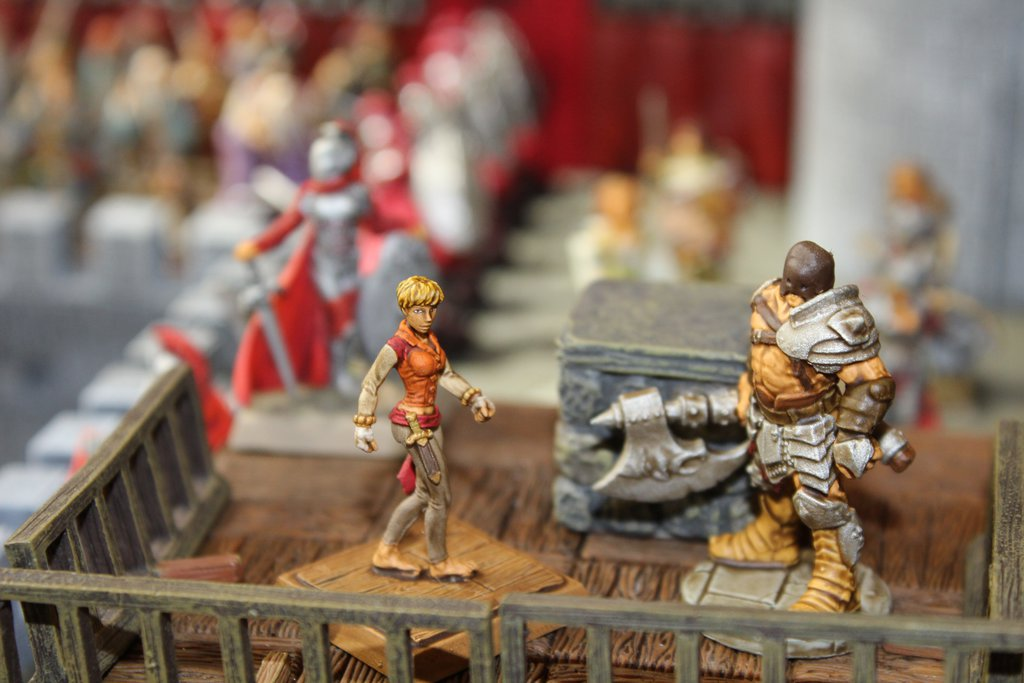
\includegraphics[width=0.39\textwidth]{images/Trinia-Sabor-facing-the-executioner-470603042.jpg}
	\caption{Trinia Sabor facing the executioner}
	\label{fig:Trinia-Sabor-facing-the-executioner-470603042}
\end{figure}



	%!TEX root = ../crimson_throne_book_main.tex
% 2014-08-02
\section{15 Sarenith 4708}

Just like the coronation three days ago Trinia's execution takes place on the terrace of the Castle overlooking Ramp Boulevard. Once more the toast of Korvosa is in attendance, for a more macabre show this time.\hyperref[fig:Quint-and-his-friends-witness-the-execution-470603218]{ Quint and his friends are among these honored guests } and, although they seriously doubt that justice is being served today, they don't see how they can stop the event. An impressive host of Gray Maidens stands guard, using their wall of silver shields to keep the visitors back. The streets below are filled with people as well, who have read about Trinia's crime and confession in today's edition of the Korvosa Herald. They do not seem to doubt the painter's confession and are eager to see her head drop. \\

\begin{figure}[h]
	\centering
	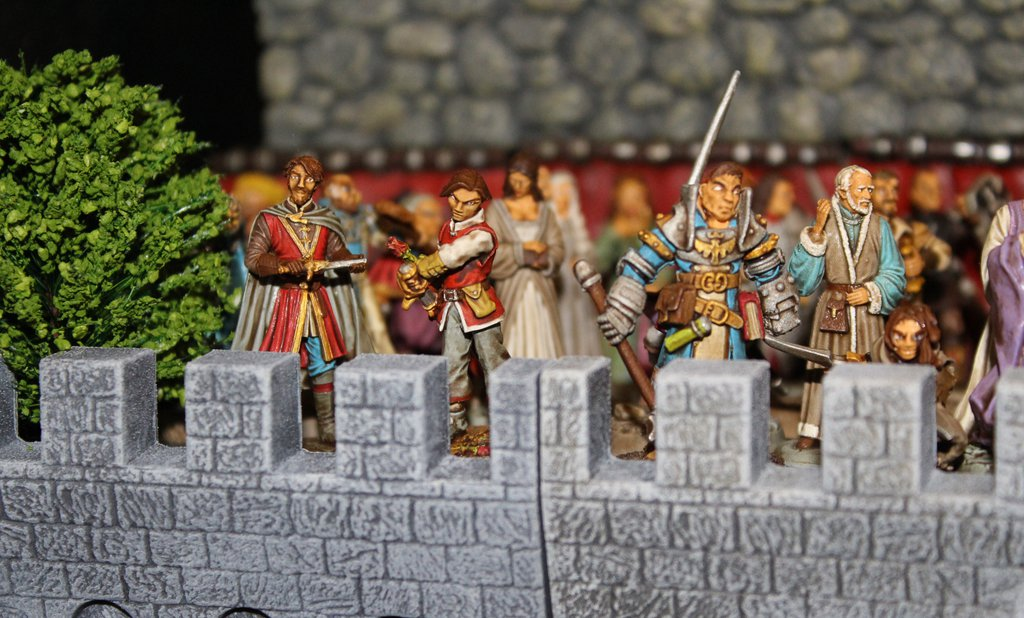
\includegraphics[width=0.39\textwidth]{images/Quint-and-his-friends-witness-the-execution-470603218.jpg}
	\caption{Quint and his friends witness the execution}
	\label{fig:Quint-and-his-friends-witness-the-execution-470603218}
\end{figure}

Drums roll as the queen emerges from the castle, closely followed by her bodyguard shadow Sabina Merrin. Having fully accepted the mantle of monarch, Ileosa carries herself with a graceful pride, showing off her beauty in a magnificent gown of green and white silk. The icy glare in her eyes totally ignores the elite that has gathered on the terrace. In her wake follows a towering, muscular man with a hood covering his face and an enormous axe in his hand. The drums suddenly change their beat to a more ominous tune as a young manacled girl with a bag over her head is herded out of the castle. Gray Maidens deliver her to the executioner's block, before pulling away the bag to reveal a\hyperref[fig:Trinia-Sabor-facing-the-executioner-470603042]{ frightened woman } who can barely keep back her tears. While one of the soldiers unlocks the shackles, another pulls back Trinia's hands and binds them behind her back with a leather cord. Then she forces the girl to her knees, her head looming over the block. \\

\begin{figure}[h]
	\centering
	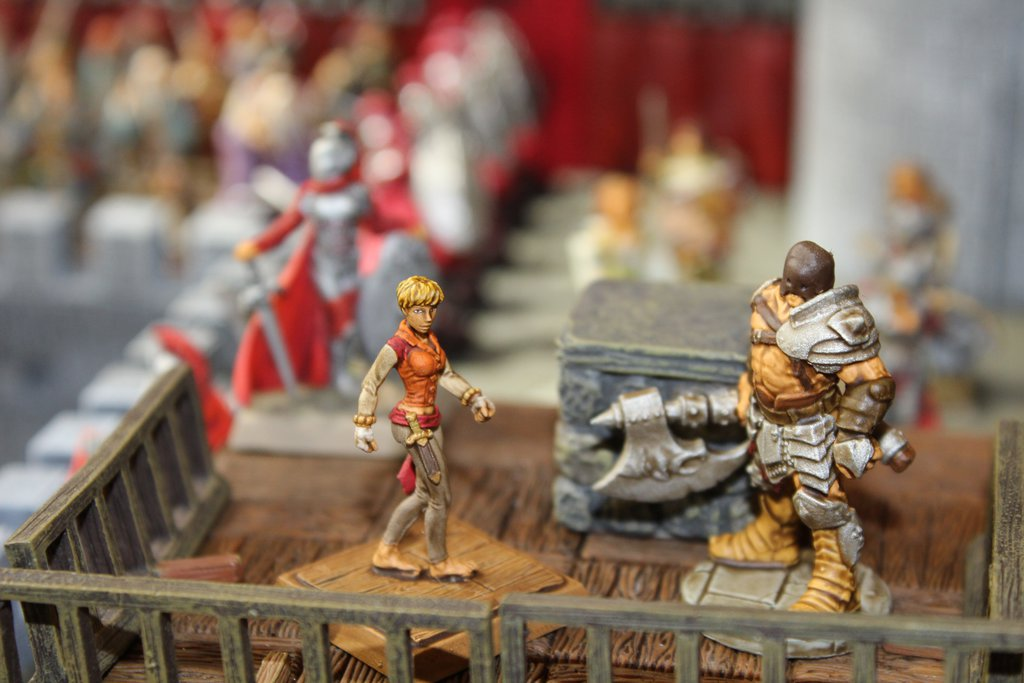
\includegraphics[width=0.39\textwidth]{images/Trinia-Sabor-facing-the-executioner-470603042.jpg}
	\caption{Trinia Sabor facing the executioner}
	\label{fig:Trinia-Sabor-facing-the-executioner-470603042}
\end{figure}

\hyperref[fig:The-execution-of-Trinia-Sabor-470602177]{ Ileosa walks over to the podium } overlooking the crowd and addresses her subjects: "Fellow Korvosans. The past few weeks have been hard on all of us. We have suffered greatly under the sea of trouble that washed over our city. I feel your suffering, for not only have I lost a beloved husband, but with each riot, each burning home, each act of anarchy and each victim my heart bled a little more. This has been a trying time for us, yet your torment is at an end. \\

\begin{figure}[h]
	\centering
	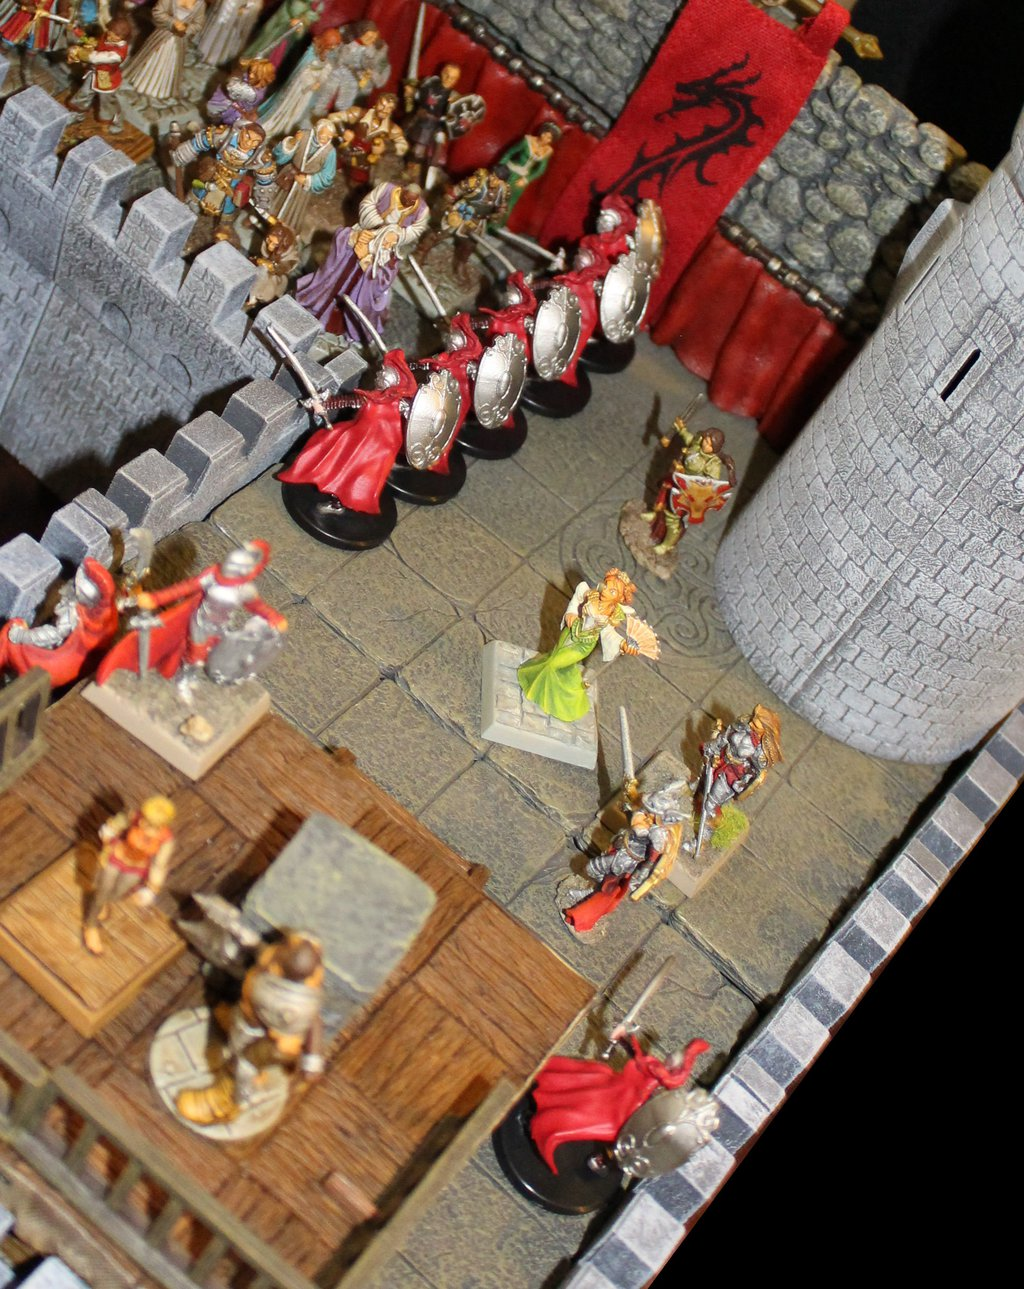
\includegraphics[width=0.39\textwidth]{images/The-execution-of-Trinia-Sabor-470602177.jpg}
	\caption{The execution of Trinia Sabor}
	\label{fig:The-execution-of-Trinia-Sabor-470602177}
\end{figure}

Before you is the cause of all this misery. Do not be deceived by her innocent nature - she is a black-hearted assassin, a seductress and a sinner, a viper amidst us all. I offer you her head as a salve against the hatred and hurt you have suffered. Her death will not rebuild Korvosa, nor will it bring back the king. Yet tomorrow will be a new dawn - a dawn over a city ready to rise from the edge of anarchy to become stronger than ever before!\\

And so, without further ado, let us usher in this new dawn with an act us justice! Off with her head!"\\

As the headsman slowly lifts his axe overhead, the crowd freezes in anticipation. His muscles bulge under the weight of the weapon. Quint, Balian, Sjo and Puk stand only a few yards away, disheartened but unable to interfere. Just as the executioner wants to swing down his axe, he gives a grunt and staggers. He lowers his weapon, reaching with his left hand to the small of his back, which is hidden from the spectators on the terrace. When he brings his hand to his face, the companions see that his fingers drip with blood. Puk then notices the flash of a slender dagger through the air that embeds itself in the headsman's right hand, forcing him to drop his weapon. Trinia raises her head, glancing up at the executioner who doubles over in pain, now revealing his first source of pain: a throwing dagger in his back. A scream echoes through the crowd: "By the Gods, it's Blackjack!"\\

From the towers of the Castle, swinging at the end of a slender crimson banner, a cloaked figure sails through the air and lands on the podium between Trinia and the axeman. As his feet touch the block where the young painter's head was meant to be separated from her body, his rapier flashes forward, slashing through the bonds on Trinia's wrists. While the girl rises to her feet, the\hyperref[fig:Blackjack-rescues-Trinia-Sabor-472558046]{ masked crusader } shouts: 'Yes indeed, Queen Ileosa! Let us usher in a new dawn with an act of justice - but true justice, not this deceit with which you try to blind Korvosa!" \\

\begin{figure}[h]
	\centering
	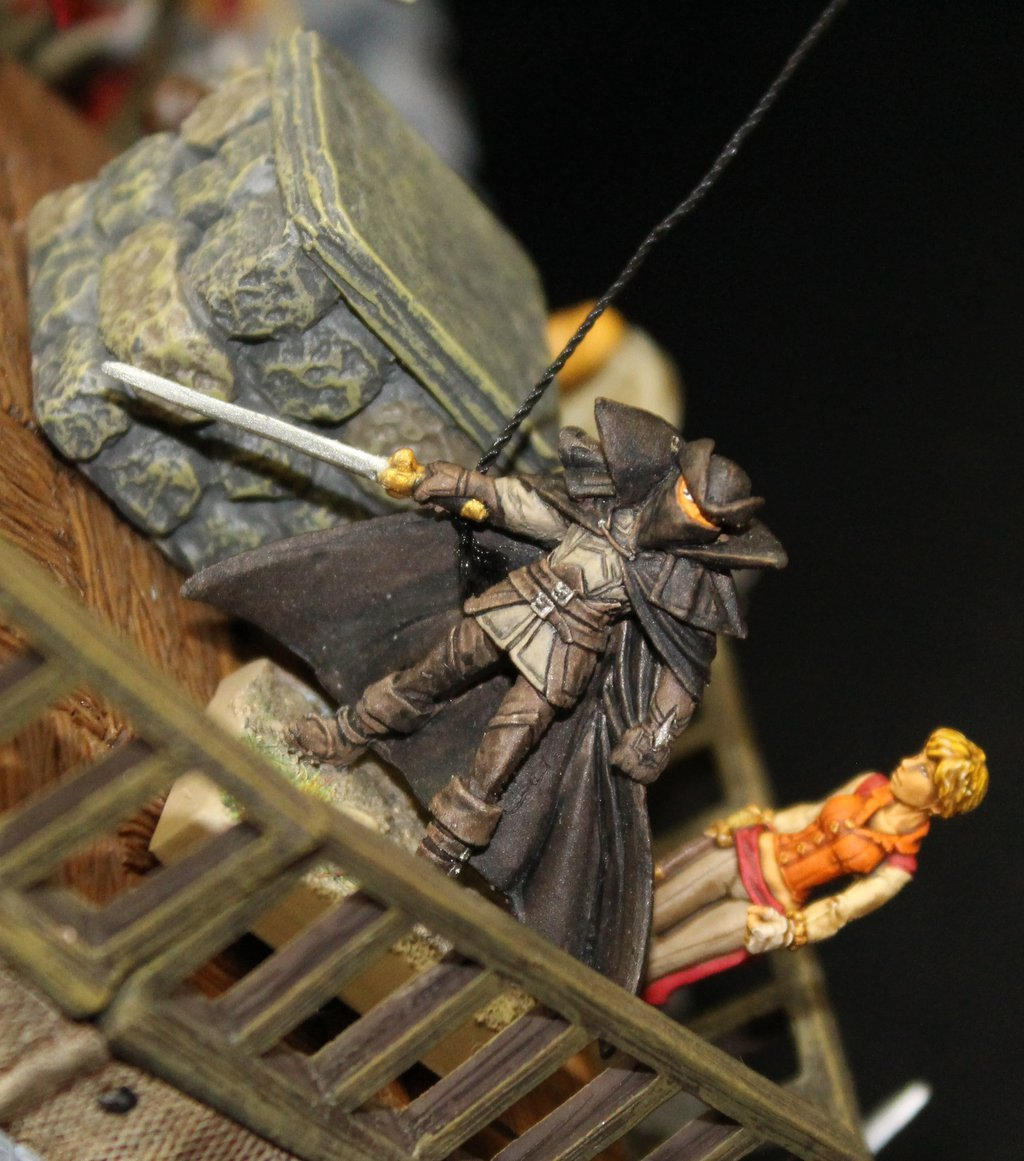
\includegraphics[width=0.39\textwidth]{images/Blackjack-rescues-Trinia-Sabor-472558046.jpg}
	\caption{Blackjack rescues Trinia Sabor}
	\label{fig:Blackjack-rescues-Trinia-Sabor-472558046}
\end{figure}

Everyone stands stunned for a moment. Then several onlookers burst into action at the same time. The queen whispers something to Sabina Merrin who quickly orders her troops to seize the assailant. Quint sees no path through to crowd and yells out words of discouragement to the Gray Maidens, using bluff to disguise his {\itshape satire} as a warning to be cautious of this skilled killer. Being a  {\itshape clumsily} brings down two female soldiers who were about the charge Blackjack and apologizes profusely, as he is  {\itshape only trying to help} . Meanwhile the executioner has regained his bearings and picked up his axe again, threatening to strike Blackjack from behind. Yet it seems like the cloaked scoundrel has eyes in the back of his head, for he jumps over the axeman's deadly chop before he quickly \hyperref[fig:Blackjack-saves-Trinia-Sabor-2-472559200]{ grabs Trinia by the arm } , ordering her to hang on. The next moment the caped crusader sails through the air again on the crimson banner with the young woman clinging to his side, first swinging back to the castle, then running over the wall to gain extra speed. As he swerves back down, he pushes off, propelling himself and his proxy to the roof of a nearby building. He glides off the tiles, but somehow manages to halt his momentum and regains his feet. Once more he looks up at the castle to see the queen flee inside. He raises his rapier in salute to the crowd on the terrace and in the streets (and possibly to the companions who aided his escape). With a swoop of his cloak he turns around and disappears with Trinia over the rooftops. \\

\begin{figure}[h]
	\centering
	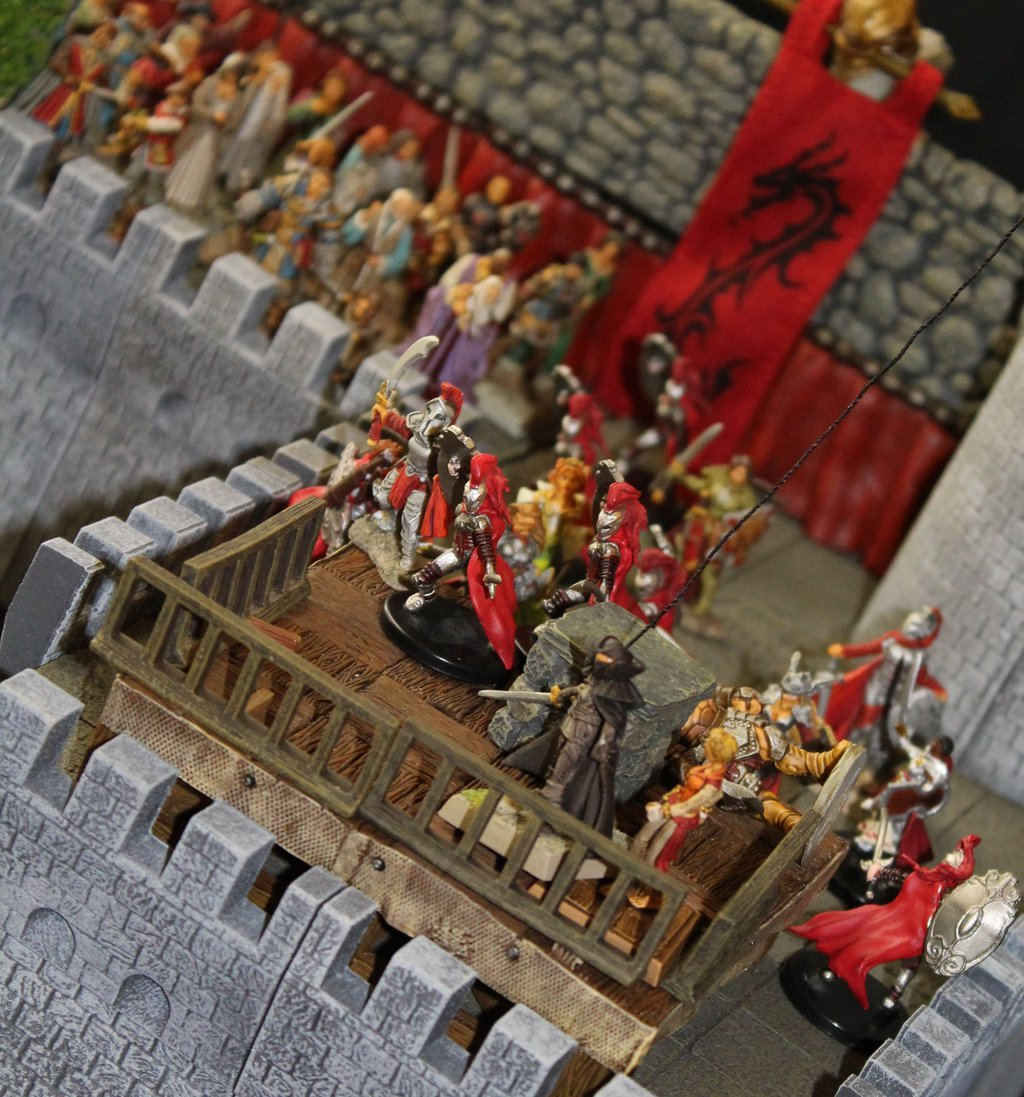
\includegraphics[width=0.39\textwidth]{images/Blackjack-saves-Trinia-Sabor-2-472559200.jpg}
	\caption{Blackjack saves Trinia Sabor 2}
	\label{fig:Blackjack-saves-Trinia-Sabor-2-472559200}
\end{figure}

Meanwhile the Gray Maidens push back the elite visitors on the terrace, ordering them to go home and showing no respect for the station of the people in front of them. Quint makes an effort to reach the executioner, offering to heal the man's wounds, but he gets driven back with the rest of the guests. He decides not to push his luck, realizing that Trinia is safe for now, and follows the aggravated nobles and dignitaries down the steps of the great mastaba that supports Castle Korvosa.\\

The companions head directly to Trinia's apartment and her friend Nisha's flat to see if either of the women are there, but find both places empty, which does not come as a big surprise. The streets in the city are filled with people who are flabbergasted by the spectacle that just transpired. Most citizens question Blackjack's motives and harbor little sympathy for his reckless rescue, as formidable a feat as it may have been. It feels like rest or peace are just not in Korvosa's cards. The Gods only know what will happen next ...\\



	%!TEX root = ../crimson_throne_book_main.tex
% 2014-08-02
\chapter{Seven Days to the Grave}

\section{16 Sarenith 4708}

A visit to Field Marshal Cressida Kroft does not yield more useful information. Quint maintains his doubts concerning Trinia's trial and confession, but Kroft can only reply that the city and the Guard are using all their resources to find the escaped girl and her cloaked rescuer. The castle has spread wanted posters all over the city, offering a substantial reward for Trinia's and Blackjack's capture: 5 000 gold sails if either of them is taken alive, half that if they are dead. Information that leads to their arrest is still worth 1 000 gold pieces. This prize money is enough to sweep most people's doubts off the table, but not the companions', who return home to ponder on how to proceed. It turns out the answer is already waiting for them.\\

Seated in a chair of their own sitting room is Vencarlo Orisini, the fencing master. He says he has picked up rumors that the companions have serious doubts about Trinia's guilt, which he more than shares. When the adventurers confirm their position, Vencarlo entrusts them with the fact that Trinia is hiding in his academy. Blackjack brought her there after saving her from losing her head. Orisini and the mysterious daredevil have worked together on more than one occasion in the past and they trust each other in times of need. Master Orisini also spent most of last night talking to the shaken young painter and has become completely convinced of her innocence. When Quint inquires how she was made to confess, Vencarlo urges him to ask her himself, tonight after sundown. That is when he wants the companions to come to his house, to hand over Trinia so they can smuggle her out of the city. The fencing master would do it himself, but his past criticism on the government has already made him one of the usual suspects, and he does not want to risk being caught and losing Trinia in the process. He asks the heroes to take the girl to a friend, who lives outside of the village of Harse, at three days travel from Korvosa. Of course, the four friends agree to help, after all, how can they refuse a lady in need?\\



	%!TEX root = ../crimson_throne_book_main.tex
% 2014-08-09
So how do you smuggle a wanted murderer out of the city? The best way is probably right under the noses of the guards. The first plan the companions come up with is to leave Korvosa as merchants. Rather than joining a real caravan as bodyguards and subsequently abandoning these people once they are outside the city, our friends deem it wise to impersonate traveling traders themselves. They could buy a couple of mules and get some goods they can sell in Harse, like salt, painted cloth or tools. Of course they would have to be disguised, which might cause a problem when trying to hide a Shoanti who is six and a half feet tall, a halfling, a dog and a young girl ... well, the plan might need some adjusting.\\

A couple of hours after sunset Puk knocks on the door of the Orisini Academy. The fencing master sees his four nightly guests inside and offers them the comfort of his living room, where they take a seat in the large sofas by the fireplace. When he calls in Trinia, the girl eyes the companions with suspicion, but Quint quickly puts her troubled mind at ease by reassuring her that he and his friends continue to believe in her innocence, a statement that Vencarlo is eager to confirm. When the bard asks Trinia why she confessed to the murder, she claims to have no memories of the fact. She remembers being taken to a cell in the Longacre building. Only hours after her imprisonment the queen herself visited her in her prison cell. That is the last thing Trinia remembers ... everything after that is a big blur, until she was thrown into another cell, somehow knowing that she had been convicted to die. The next 24 hours awaiting the execution had been the most desperate in her life.\\

Vencarlo Orisini asks the companions to smuggle Trinia out of Korvosa and escort her to a good friend who lives outside of the village of Harse, on a horse ranch. His name is Jasan Adriel and he and Vencarlo used to be in an adventuring company together more than twenty years ago, called the Blackbirds. The fencing master also has a coded letter for his friend, which he hands to Quint. He encourages the four heroes to act fast: as a known critic of the government Orisini is on the list of the {\itshape usual suspects} and Trinia remains in danger as long as she stays under his roof. Some guards already did a cursory search of his academy today and he suspects they will be back soon for a more thorough investigation. He also gives the companions 500 gold sails when he learns they will try to impersonate merchants, but still need to buy pack animals and merchandise. Before they leave Vencarlo warns the companions to be very careful: the Guard is looking everywhere for Trinia, the Sable Company controls the skies and the river and the sword master has even picked up a rumor that the accursed Hell Knights have been called back to aid in the manhunt. The companions hide Trinia in the old fishery for the night and finally decide on a different plan to get her out of the city: they will leave as themselves, with Trinia taking the place of Quint, whom she resembles most closely physically. The bard will disguise himself as a regular John Doe and leave Korvosa on his own, meeting up with his friends outside of the city walls. To facilitate Trinia's impersonation of him, Quint hits the town heavily that night, making sure to show up in every bar that frequently hosts soldiers of the Guard, buying them drinks and getting {\itshape really drunk} with them, all the while complaining about Puk. Apparently his small friend wants to leave civilization tomorrow to head to the backwater halfling hole of Heavenguard for a someone's birthday. How dull is that? And of course the little bugger promised his cousin that the great Korvosan performer Quintillian would accompany him, leaving Quint no choice but to join him on this uncomfortable trek into the wilds ... The bard also picks up the general sense that most Korvosans believe Trinia to be guilty. It turns out that he and his friends certainly succeeded in restoring faith in the monarchy over the last few weeks, as people tend to trust Queen Ileosa now and share her hate for the late king's killer! 

	%!TEX root = ../crimson_throne_book_main.tex
% 2014-08-09
\section{17-19 Sarenith 4708}

The next morning Quint helps Trinia into his own clothes and fixes her face and hair to make her look like him. As she will be playing a hung over bard, she will be able to keep to the background and hang her face low. Meanwhile Sjo writes a letter to Larella Semyr, his beautiful priestess girlfriend, and another missive to Field Marshal Kroft. He asks the boys to deliver the first note to the shrine of Shelyn, but keeps the second letter on his person, taking it with him as he heads for the Bloodsworn Gate with Puk, Balian, Spyder and Trinia. There is a small line of people waiting to get out of the city, and the guards do a scrutinizing job of checking everyone who leaves. When the companions are up, the soldiers visibly relax: these are the trusted heroes of the city! They chuckle at the hung over bard and easily accept Sjo's explanation that they are traveling to Heavenguard for a birthday, you know how halflings like their parties ... The Shoanti also hands the guards the letter for Kroft, asking them to deliver it to their commander since he didn't have the opportunity to inform the Field Marshal of his and his friends' absence himself. Feeling honored the guards quickly let the heroes pass. Quint has no trouble slipping through the checkpoint a couple of minutes later - as no one is looking for a single man - and meets up with his friends at the next crossroads.\\

The journey north takes three days, during which Trinia proves to be a spirited little girl. Despite the traumatizing experience she has been through, she is excited and thankful to have escaped with her life. She recounts with gusto how she fled with Blackjack over the rooftops of Korvosa, down small allies and even through the sewers. The caped crusader knew his way around the city well and led her unerringly to Vencarlo's fencing school in Old-Korvosa. While she waited outside in the shadows for a few minutes, Blackjack went inside to convince his friend to take in the girl. She witnessed their brief but heated discussion, before the grey-haired swordmaster invited her in and offered her his protection. He turned out to be the perfect gentleman and host, worrying over her like a father-figure.\\

Trinia suspects that Neolandus Kalepopolis, the missing seneschal of Castle Korvosa, is behind Blackjack's mask. His position allows him to dethrone an illegitimate or unjust monarch in times of need, but that power also makes him a target of such an individual. Trinia is convinced that Queen Ileosa is a false and dangerous snake who forced the seneschal into hiding. Since his life would be in danger if he appeared publicly, Kalepopolis had to resort to his Blackjack alter ego to fight the treacherous usurper. Being an ex-officer of the Sable Company, Neolandus Kalepopolis certainly has the skill to be the caped crusader, heck, he's probably even hiding in the Great Tower, the headquarters of the black garbed guards. That would definitely explain why commander Marcus Endrin has been so suspicious of the new queen as well ...\\

The young painter also unfolds that painting was not her first profession of choice. Being the daughter of a Varisian couple of traveling acrobats, she originally trained in her parents' skills at tumbling and jumping, which explains why she was so agile fleeing from the companions over the shingle rooftops. When her parents froze to death during the terrible hunger winter six years ago, she decided to quit her life on the road and focus on another talent: painting. She settled down in the poorer parts of the city and made enough to survive, although she admits that she is not very good with money. She never had a lot, but whenever she had some, she spent it quickly, not only on herself, but also on her neighbors, since there were always people around who needed it more than she did.\\

The companions can also witness with their own eyes that the Korvosan Guard no longer patrols the Korvosa's holdings outside the city walls, although they do not run into any of the highwaymen that are supposedly plaguing the countryside.\\

By the end of the third day, the travelers reach the Falcon River and take the ferry across the water. They ignore the town of Harse completely and head straight for Blackbird Ranch, some thirty minutes north of the village, off the beaten track. The horse ranch sits comfortably in the cleft of two low hills topped with copses of fir trees. A barrel-chested man, flanked by two youths, greets the companions as they approach. His bow is strung, but hangs idly over his shoulder. Still, it looks like it is within easy reach. The man's initial apprehension instantly evaporates when he learns that his friend Vencarlo sent these travelers to his doorstep and Quint hands him the fencing master's coded letter as proof. He warm-heartedly welcomes his guests into his home. Blackbird Ranch is a large place, but also houses a large family: Jasan Adriel himself, his wife Lisanna, his sons Ted, Gerald and Bruno and his daughters Mari\"en and Romy. The rancher takes the visitors to the basement, where he keeps a couple of spare beds and brews his own beer, which he offers freely.\\

Jasan informs about the situation in Korvosa and when he learns of all the recent trials and tribulations, he explains that such troubles are exactly why he chose to relocate down here and not in the city. At least here he can talk frankly without worrying about his family, because, just like Vencarlo Orisini, Jasan can be quite critical about people in charge and likes to speak his mind.\\

After a couple of pints the retired adventurer also talks about the past he shared with Orisini. The two of them were members of an adventuring party known as the Blackbirds. They broke up more than two decades ago over an unfortunate argument involving the rights to treasure looted from a dwarven tomb - while Jasan and Vencarlo wanted to return the weapons they recovered from the haunted grave to the dwarven offspring in Janderhoff, the others in the group wanted to keep the loot and sell it in Korvosa. The conflict came to blows and in the end Jasan and Vencarlo opted to retire from the adventuring business altogether. The remaining Blackbirds vanished without a trace in the obscure dungeons below Kaer Maga not one season later, so both the ranger and the sword master counted themselves lucky at having quit while they were alive. The two former party members have always stayed in touch, writing each other as often as possible, using the secret code they developed in their adventuring days, more out of fun than any real need to hide their messages, although it allowed them to be critical of Korvosa's government without the fear of anyone else reading about it.\\

Since the companions changed their plans on how to get out of the city, they never needed Vencarlo's money to set up a merchant guise, so now they offer the pouch to Trinia. The girl sees no need for the gold while she is hiding in a basement and suggests to give the money to Jasan instead. Although the ranger is pleased with his guests' generosity, he responds that he requires no payment for helping his best friend and only agrees to take the money if the companions accept riding animals in exchange. Since Jasan Adriel breeds some of the finest horses around, this sounds like a great deal, but it will have to be concluded tomorrow, as the hour has grown very late.\\



	%!TEX root = ../crimson_throne_book_main.tex
% 2014-08-09
\section{Sarenith 4708}

While Jasan takes his guests around the ranch to select his best mounts, a simple farmer woman stumbles onto the porch of his house. She looks desperate. Jasan hurries over, explaining she is his neighbor Mia, and inquires what is wrong. Mia falls into his broad arms crying and sobs that her husband Barold and her boys did not return from the field last night and are nowhere to be found. Jasan asks his wife to see to Mia and happily accepts the companions' offer to join him to Barold's farm. Trinia wants to come as well, but no one feels comfortable exposing her to potential danger, so she has to stay at the ranch.\\

Jasan leads his new allies to his neighbor's place, some fifteen minutes away. The farmhouse is much more modest than Blackbird Ranch, but still looks like a decent dwelling. Jasan has a quick peek around and then heads to a field down the path. "It seems like they were working the northern field", he states as he takes the companions further. While he gets off his horse to check for tracks, Puk notices a throwing spear in a nearby tree. When they move in to examine it, the companions find an unconscious man with a bloody wound to the head in the bushes. It is Barold, Jasan's neighbor. After he has received some healing, he explains that he and his two sons were surprised by four mean-looking bugbears last night. They knocked him out and left him for dead, but there is no trace of Vern and Sender, his sons, or Bianca, his cow. Jasan orders his horse to take Barold to the ranch and continues on foot, following the tracks of the bugbears into the wood, who obviously made no effort to hide their footprints.\\

After two hours the adventurers happen upon an open spot in the forest, backed by a rocky outcropping with a cavelike entrance. Barold whispers it is an old Shoanti tumulus, from back when the barbarians still roamed the lush lowlands and buried their dead in hillside graves, a custom they have long since abandoned as the inhospitable Cinderlands are more suited for burning the deceased than burying them.\\

Puk scouts ahead and spots four bugbears around a campfire in front of the tumulus entrance. A cow is tied to a tree off to the right. The companions waste no time and take the feral brutes by surprise. Puk and Balian charge the creature to the right, inflicting bloody cuts, but he still stands and returns the favor by viciously clubbing Balian with his morningstar. Sjo picks out the biggest warrior, who is wielding a morningstar in his right hand and a light hammer in his left, and casts {\itshape hold person} on him, freezing him in place. Then the Shoanti moves in to engage the left bugbear. Quint demoralizes the opponents with his  {\itshape satire} while Jasan peppers the creatures with his arrows. The wounded beast facing Balian is felled with one more mighty blow and the two other bugbears get beaten, bitten and shot from various angles while getting in only minor hits themselves. As they both sink to the ground dead, their leader snaps out of his paralysis and opts for the safety of the tumulus. Despite his hulking build he is no fool, realizing that facing five opponents out in the open spells certain death. 

	%!TEX root = ../crimson_throne_book_main.tex
% 2014-08-14
After some quick healing the companions enter the tumulus into which the burly bugbear disappeared. Quint supplies some much needed light with a simple spell cast on his buckler. A tunnel leads under the hill, immediately splitting off in three directions. A quick examination of the left and right passage reveals two round rooms, where the moisture in the walls has worn away any marking that might have once adorned them. The chamber to the right is being used as a private bedroom with some hides on the ground and a makeshift shrine of old bones and skulls; the room to the left has a big hole in the ground which serves as a waste pit and toilet.\\

The main tunnel leads deeper into the tumulus and provides access to the ancient burial chamber, with eight alcoves lining the walls. Four bugbears are waiting for the heroes in here, one of which has taken up position on a stone table in the middle of the room. He forms the perfect target for Jasan's first arrow, which kicks off the fight. A bugbear in the back of the room seems to master some magic and reacts by casting a spell on Balian. The ranger feels his breastplate growing hotter, but Sjo's quick thinking provides the perfect 'antidote' for his scorching {\itshape heated metal} in the form of  {\itshape resist energy} . Quint demoralizes the opponents with another  {\itshape satirical} performance, while Puk jumps into the fray on top of a barrel. His tiny blade does not penetrate his adversary's armor, but the halfling has put himself in a precarious position, taking two firm hits from the bugbears that face him. Balian and his dog Spyder also charge forward, but their attacks go wide. Despite his fierce growls and sharp teeth, the canine is no match for the bugbear leader, who steps in and mercilessly hammers the dog with two main hand hits and one off-hand swing. His morningstar and light hammer drip with blood as the dog drops to the floor. This hulking creature delivers a mean punch, Sjo understands. His  {\itshape hold person} outside the entrance on this brute was even more valuable than he realized. He tries the spell again, but this time the hairy beast resists his magic. Meanwhile Balian draws his first blood of the fight by cleaving through the two bugbears that are pressing Puk. The halfling cannot get into an advantageous position without putting himself in even more risk and takes a defensive stand, which makes his opponents miss their attacks. In the meantime Jasan fires another arrow in the bugbear on the stone table, who just received some healing from the druid in his back.\hyperref[fig:Shoanti-tumulus-475539806]{ With Spyder down, Balian is now the leader's next target } : the hulk steps forward and pummels the ranger twice with his morningstar, reserving his backhand swing for Quint. The creature snorts out a hysteric laugh to celebrate his success. Quint feels that it is high time to swing the momentum of the fight and decides to use another of his tricks. He pulls out his whip and lashes it around the ankles of the bugbear on the table, pulling the creature's legs out from under him. Balian interrupts its attempt to rise with a deadly strike and takes its place on the stone table, finally gaining a flank with Puk on the other bugbear. The halfling takes full advantage of this position and pulls out two vicious sneak attacks that cut the unfortunate mutt down. At last the battle seems to turn for the better. Sjo engages the druid, who pulls out a sickle that glances off the Shoanti's plate. The fire-wielding healer retorts by spewing forth a sheet of flames that scorches both enemies that are left standing. Still, the fierce bugbear leader does not give up and continues bashing Sjo and Quint. He also proves to be very hard to hit, so the fight  {\itshape ain't over yet} . Sjo uses heroic inspiration (we use hero points)  {\itshape hold person} , but again the towering monster resists. Next Quint also fails to trip him. Puk and Balian now flank the creature, but the halfling cannot get through its defenses. Balian fares better and cuts deeply into its flesh. The ranger continues the arc of his blade and slices through the druid as well. Despite the bleeding gash, the leader seems unimpressed and pushes the attack, wounding Balian, Puk and Quint with his whirling weapons. A second attempt by Quint to topple the bugbear champion succeeds, leaving the being prone between the bloodthirsty halfling, the fuming Shoanti and the enraged ranger. The companions exploit the opportunity to the fullest, literally hitting their enemy while he's down. Balian hacks heavily into the hulk's frame and Puk's flashing blades finally finish the brute off. The druid is helpless against superior numbers and swiftly follows his brethren to the grave. \\

\begin{figure}[h]
	\centering
	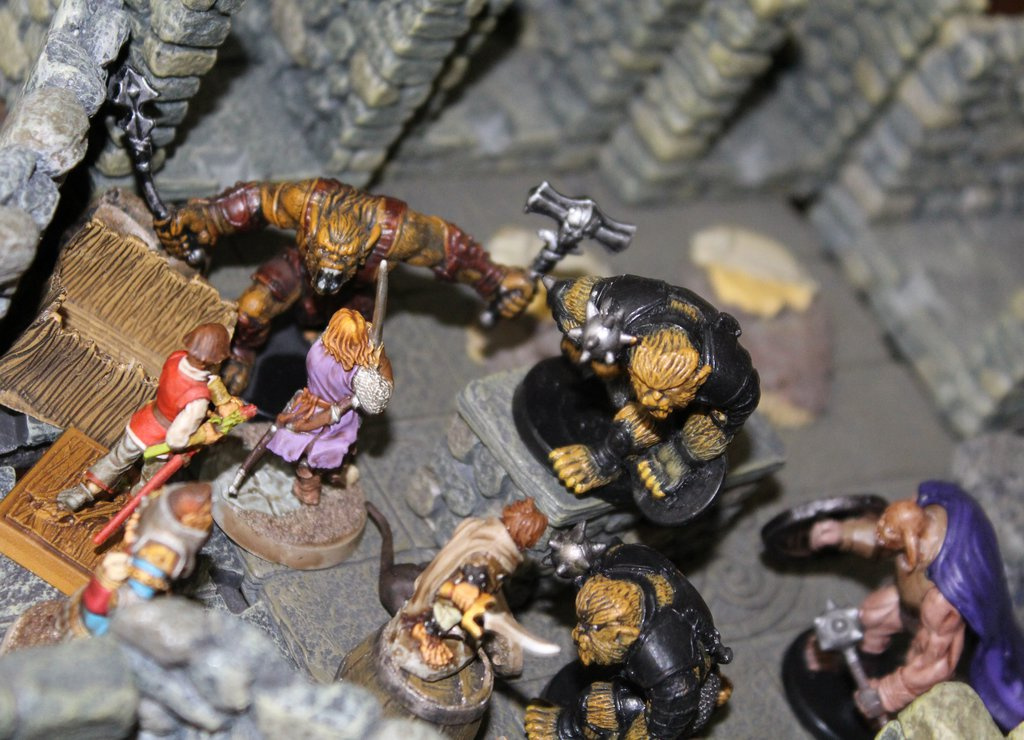
\includegraphics[width=0.39\textwidth]{images/Shoanti-tumulus-475539806.jpg}
	\caption{Shoanti tumulus}
	\label{fig:Shoanti-tumulus-475539806}
\end{figure}

The companions take a few moments to catch their breath. As they are healing up, two young voices call out from one of the alcoves that has been blocked by a heap of stones. Farmer Barold's sons, Vern and Sender, have been locked up there. They are overjoyed when their rescuers inform them that both their father and cow Bianca are still alive. Puk leads the search of the complex and unearths a hefty pouch with gold, while Quint discovers that the bugbear leader's studded leather is magical and Sjo finds an old Shoanti pendant around the druid's neck. The engraved runes spell {\itshape Storval ekbitel nalharest} , which is Shoanti for  {\itshape We walk the land as brothers} . Other markings in the stone table identify this tomb as a Shundar-Quah grave, another of the Shoanti tribes that once roamed this country. Sjo is disgusted at the bugbear sacrilege of this holy place and asks his friends to help him remove them from the tumulus. The companions drag the cadavers of their enemies outside and build a funeral pyre. They also take out the bugbears' supplies from the tumulus and give them to Barold, along with 100 gold sails from the loot. This small gift is a true fortune for the simple farmer, who is very grateful for the safe return of his children, his cow Bianca and the heroes' generosity. It is already a few hours past noon when the companions head back to Korvosa. Fortunately they now have horses, so they should be able to make up for the time they lost.\\



	%!TEX root = ../crimson_throne_book_main.tex
% 2014-09-06
\section{22 Sarenith 4708}

Late in the afternoon the companions arrive back at the gates of the city, making sure to approach the city from the east rather than from the north, as if they came from the halfling town of Heavengard. While soldiers are still strictly checking everyone who's leaving or entering the city, the heroes get in easily and find the atmosphere inside Korvosa much more relaxed than a couple of days ago. Today is the 22nd of Sarenith, which is a popular local holiday known as Riverwind Festival. At the start of summer the winds shift for a few weeks, bringing down a cooling breeze from the Mindspin Mountains. This break from the stifling heat is typically celebrated with games and drinking and the festivities are already in full swing.\\

The companions head straight for the villa to freshen up and stable their new mounts. Korwick, Heldrin and Mouse are excited to see the horses and are eager to take care of them, but Sjo can tell that they have been taking it easy while he was away, as the house is a bit of a mess. He has the boys help him prepare a bath so he and his friends can clean up before they dive into the streets of Korvosa to join the festival. Balian convinces his comrades to compete in a friendly tug o' war competition against four baker's apprentices. The companions are almost taken by surprise as their opponents throw all their strength and weight into an early attempt at victory, but they manage to turn the tide and end up pulling the four flour covered men into the muddy ditch in the middle.\\

Quint and Sjo also chat with some of the bystanders and find out that the search for Trinia raged quite heavily until yesterday. Today's 'holiday spirit' apparently changed the mood and things are starting to feel normal again. The only exception are the Hell Knights, who've been conducting their own search, automatically expecting everyone to cooperate freely and rough handling anyone who doesn't. People are also saying that a ship burned out and sunk in the middle of the river yesterday, without ever making it to the docks.\\

The highlight of today's festivities is the Riverwind Race. Runners make their way through the streets of the city from east to west, mirroring the direction of the wind. The race starts on North Bridge and makes for Jeggare Circle over Norhtgate Avenue. From there Dead Shoanti Way and Academic Avenue take the contestants to the finish in the shadow of the Acadamae. Balian and Quint give it a shot and join the contest. Quint worms himself into the front row between last year's top six: two members of the guard, Cressik and Ringo, a ranger and a stable master, called Nalia and Vardin, the son of a trader, Daramir and a tall Shoanti, Portok Eagle-Eye, who was the winner of the previous edition.\\

Quint immediately sprints into first position, but is quickly overtaken by the guard Ringo who stays in front until Jeggare Circle comes into view. By that time Quint is already lagging behind, but Balian is dividing his efforts more evenly and never stays more than a few yards behind the person in the lead. Then Cressik, the other guard, takes over and sprints away from the competition. Ringo and Balian do their best to keep up, while the rest of the playing field loses more distance. It looks like Cressik is in for the win, but he overestimated his own vigor and slows almost to a halt in the final stretch. Ringo spurts by his colleague, leaving him to bite his dust and taking Balian by surprise. The ranger pulls out a final sprint and ends up a couple of yards short of the winner. Still, he lands a very respectable second place. Nalia the ranger comes in third and Portok the Shoanti takes the fourth place. Cressik ends up fifth and Quint is sixth, although he left quite a gap.\\



	%!TEX root = ../crimson_throne_book_main.tex
% 2014-09-06
\section{23 Sarenith 4708}

The next morning sees some commotion in the kitchen. Heldrin and Korwick are accusing Mouse of having placed a dead rat under the table, something which the smallest of the three boys vehemently denies. Sjo and Balian examine the rodent and conclude that it died either from disease or poison. They bury the tiny cadaver in the garden. Sjo also purifies the food, just to make sure there is no poison, but even that cannot freshen stale bread, so they head to the baker's for some fresh loaves instead.\\

In the street they run into Grau Soldado, their sergeant friend from the Guard. He looks a lot cleaner than when they last met him, when he was drunk and depressed for having lost a few of his men and his brother in the riots. Still, he has an air of worry about him as he hails over the companions: "Friends, I was just looking for you. My little niece has come down with something. She's covered in red spots and can't hold down her food. She was very feverish all through the night and, to be honest, I'm concerned. Her mother wants to take her to the Bank of Abadar, to be cured, but she cannot afford the fee. I remembered your kindness and skill and was hoping you could help her out. Little Brienna is such a sweet girl. Can you make her better?"\\

Sjo replies that he does not master magic to cure diseases, but he will certainly have a look at the girl to see if there is anything he can do to help. The companions follow the guard to Trail's End. On the way over there Grau expresses his admiration for his sister-in-law. Being a single mother with three children is hard and everyone has to chip in to make ends meet, even little Brienna, who cleans houses in North Point. Grau visits them a few times a week to ensure they are safe and have everything they need.\\

When they arrive at the house, Grau's nephews are playing quietly in the living room. Tayce, Grau's sister-in-law, is upstairs with her daughter. One corner of the ground floor serves as the kitchen. A man in Abadarian garb is working at the stove, brewing some concoction that smells of cinnamon and anise. His skin is tanned, but not quite as dark as his high priest's, Darb Tuttle, who is a full-blooded Vudran. Upon seeing the man Grau is obviously displeased and rushes upstairs. Puk and Balian overhear him scolding Tayce for racking up a bill with an expensive and worthless healer when he said he would handle things.\\

Quint and Sjo head over to the priest of Abadar. Quint greets him in Vudran and he replies with a smile. He says his name is Ishani Dhatri. He is trying to help, but he has trouble recognizing the combination of the girl's symptoms and fears she might be suffering from a new disease. He is not allowed to use his healing magic, as that requires a fee to the Golden One which these simple folk cannot afford. So he's making due with his mundane healing skills. Sjo picks up that Ishani feels guilty about his church's doctrine and is doing what he can within the rules. He suggests having a look at the girl himself and goes upstairs with Balian to see Brienna.\\

The creaky steps open up into a bedroom loft above the main room of the house. A young girl with auburn hair lies in a big bed, her slight form dwarfed by the size of the mattress and the pile of pillows. Splotches of angry red rash cover her face and arms, appearing in irregular shapes and sizes. Her restlessness is interrupted by a violent fit of hacking coughs that jerk her entire frame, lifting her off the bed. The spasm passes, dropping her back in the sheets, but seemingly having done little to ease her breathing. Sjo and Balian examine her more closely and conclude that she will probably die within two or three days if she does not receive proper treatment. Sjo can already ease her suffering a bit by magically restoring some of the stamina she lost. He also tends to the rash on her skin and applies the ointment that Ishani made.\\

Since he can offer no help here, Quint decides to consult the library in the villa to see if he can find out more about this disease. The symptoms seem to coincide with those of a rare disease that was reported a few years ago in soutwestern Varisia, in a small town along the Lost Coast, Sandpoint. {\itshape Vorel's plague} put much of the town in bed sick, but despite its fierceness, it was rarely lethal, so almost all those infected survived. Quint hopes Brienna will survive as well, but remembering that Sjo gave her only two to three days if she didn't receive healing, has him worried. 

	%!TEX root = ../crimson_throne_book_main.tex
% 2014-09-06
My players hated Ishani, because he couldn't heal Brienna. I tried point out that it wasn't that he couldn't it was that he was forbidden from doing so. If he tried, the magic wouldn't work unless he was paid for it because that's one of Abadars decrees.\\

Still, despite all that, they blame him, Ishani, instead of Abadar. It's carried far enough that they don't allow clerics or NPCs of Abadar in their campaigns except as antagonists.\\



	%!TEX root = ../crimson_throne_book_main.tex
% 2014-09-07
My players weren't exactly keen on Abadar's policy either, although they did sense that Ishani feels the same on this particular point. So they don't blame him, but the church.I do like how priests of Abadar have actually become bad guys in your group, while they are nothing more than modern day capitalists, so we should all be familiar with this kind of thinking. 

	%!TEX root = ../crimson_throne_book_main.tex
% 2014-09-20
Sjo, Balian and Puk meet up with Quint and head to North Point to talk to Brienna' employer. While making their way across the city, Sjo takes the Harrow deck in his hands to consult Zellara's ghost about the strange disease. He gets a mental answer that she is not familiar with it, but maybe a new reading of the cards later today will offer some insight. When they reach the address where Brienna cleans, Sjo talks to the lady of the house. She has no symptoms and seems to be mostly worried about how long Brienna will be out. Asking around in the neighborhood does not unveil more information about sick people.\\

The companions also cross the bridge to Old Korvosa to pay a visit to Vencarlo Orisini. When the fencing master sees them arriving, he ends his lesson prematurely and sends his students off to clean up. He is very pleased to learn that Trinia is now safely in Harse with his old friend Jasan and thanks the four young men for their help. In fact, he has a reward for them. A long time ago he and Jasan were members of a band of adventurers, but they parted company with the Blackbirds over a conflict about what to do with the loot from an ancient dwarven tomb. While their friends decided to keep the treasure, Vencarlo and Jasan went to the city of Janderhoff to return their share of the loot to the dwarves. The Janderhoff people greatly appreciated their gesture, but still allowed them to keep what they had found. In Vencarlo's case it was a weapon, but preferring blades himself (especially the rapier), he never used it. Still, he never got rid of it either, promising himself that he would not sell it for profit, but rather put it to good use. Now he has found such a purpose in Sjo, who is well trained to wield it. Vencarlo disappears upstairs for a couple of minutes and returns with a heavy mace in his hands. Sjo is a bit shy about accepting it, but then he promises to use it to help defend the city. The metal feels quite cool to the touch as the weapon turns out to be made of cold iron.\\

That evening, after dinner, Sjo pulls out the Harrow cards and summons Zellara's ghost for a reading. The fortuneteller feels that Sjo's earlier questions about sickness and health would be best suited with theshield  {\itshape the trumpet} , which represents an archon blowing a horn in an overt declaration of power. This display of force clearly calls for Sjo to face the dire situations ahead with similar confidence. Quint picks  {\itshape the brass dwarf} which shows an azer who is unaffected by the flames that surround him. Likewise Quint will have to find the strength to withstand whatever dangers will cross his path. Balian's card is  {\itshape the waxworks} , a place of helplessness which dangles a bound man above a steaming vat of molten wax. If he is plunged into the boiling goo, he will be frozen in place for ever in eternal torture. Balian will have to be extra careful not to be caught in the inability to move or act himself, so this card serves as a dire warning. Despite his small build, even for a halfling, Puk draws  {\itshape the mountain man} , signifying that he might be a giant amongst men. The towering giant also stands for a huge force that is very hard to control, so hard even that it might be wise not to get carried away by it, if you want to survive its destructive power. Next Zellara puts the shield cards back in the deck and performs a full reading for everyone. Puk still needs to come at peace with his past, as shown by both the {\itshape inquisitor} and  {\itshape juggler} card. There is tragedy that he still hasn't fully accepted, as if he can't admit the truth about his own involvement, not even to himself.  {\itshape The wanderer} in his present acts as a collector of things that are valuable to him, even when others consider them useless. Puk has also shown a great knack for acquiring items, as he is possibly the best equipped member of the group. His days to come turn up two misaligned cards.  {\itshape The rakshasa} reveals the threat of a force that wants to enslave the bodies or minds of others, but the fact that it is in the opposite corner indicates that Puk might play an important part in casting off this enslavement. The empty throne suggests that this threat originates in an ancient past, whose restless ghost reaches out to the present. Balian's past is under the sign of the winged serpent, pointing out that the ranger has always known when the time to act had arrived. Apparently Puk is not the only giant amongst men, because {\itshape the mountain man} in Balian's present reveals that he is an equally impressive force.  {\itshape The beating} also indicates that the companions are constantly being threatened from multiple sides, making it hard to tell who is a friend and who is the enemy. The future turns up the  {\itshape unicorn} and  {\itshape the hidden truth} , although the third card in this column, which remains uninterpreted, is  {\itshape the idiot} , which obviously elicits some snickering from Balian's friends. The unicorn stands for someone who will offer help to uncover the real truth, although the hidden truth predicts that this truth might be something you had rather not known. Quint's cards reveal little. Just like in his first reading he does not draw a single card from the suit that blesses today's session.Characters gain a Harrow point for every card they draw from the chosen suit, which was  {\itshape The dance} in the bottom row of his past seems to indicate that Quint has always struggled to fall in line and follow the pace that was imposed on him.  {\itshape The tyrant} in his present is a ruling force that could be harmful to all, but the fact that it is in the upper row suggests that Quint is capable of detaching himself from that force.  {\itshape The big sky} in the bottom row warns that casting off the shackles of one master might quickly see new manacles from another lord.  {\itshape The crows} in the future are a dangerous bunch of enemies who violently take what they want and destroy that which is loved. The companions might be the only ones who can avert the threat of these long-beaked villains. Sjo has the misaligned {\itshape demon's lantern} in his past, as a sign that he had a hard time finding his true path, but the card's position suggests that he finally saw the light and he is on the right track now.  {\itshape The theater} in his present is misaligned as well. Sjo continues to play his part in the playhouse which is life, but he has to be careful to remain true to himself, so he doesn't play the wrong part. The future cards have a true match:  {\itshape the uprising} . A force stronger than the companions threatens to grab the city in its clutches. The crown on the pitchfork of the rebel in the drawing signifies an overthrowing of that force, whatever it may be ... 

	%!TEX root = ../crimson_throne_book_main.tex
% 2014-09-20
\section{24 Sarenith 4708}

When the companions walk down the street the next day, they see dead rats everywhere. People claim that they saw rats dying under their eyes. The animals convulsed in desperate spasms until they stopped moving. Asking around in the temple of Pharasma, our friends learn that half a dozen people have come in sick today with the same symptoms as Brienna. Sjo wants to swing by the Shoanti camp to give Thousand Bones the pendant he found in the Shundar-Quah tumulus. He is surprised to find out that the visitors from the Cinderlands have left town. Gaekhen's family was very angry about his death and the defilement of his body. There were also rumors that the Shoanti on the Storval plateau are gathering for war and Gaekhen's father was eager to join them, while Thousand Bones felt his mission should take him there as well, but then with the purpose of trying to prevent such a war.\\

Puk and Sjo use the privacy of the old fishery to examine some dead rats. Puk shaves them so Sjo can study their skin. They also have red spots, which have even turned into terrible sores with pus and blood. They clearly died from the advanced stages of the same disease that some citizens have contracted. The companions scour the pubs in the harbor to find out more about the ship that sank in the river, fearing it might be connected to the sick rats. There is no sign of other dead animals, the fish and birds all seem to be unaffected. If anyone knows more about the ship, it's the Sable Company. There were some hippogryph riders in the air when the vessel went down.\\

Since Balian is not the smoothest talker, he chooses to sit at a quiet table while his mates are gathering information. As he is enjoying his drink, he sees a shapely woman approaching. She is very beautiful, has a tanned skin and shiny dark hair. "You're Balian, one of Korvosa's new heroes, are you not?" she smiles while she bends forward, offering the ranger a peek into her cleavage. "I would like a word, but you have to promise me not to get mad and let me finish." Balian sighs, suspecting that this is the Vudran schemer he and his friends have been looking for.\\

"Our paths have crossed in the past, although we never actually met", she continues. "My name is Selena, but you already guessed that, I suspect. I hope you give me the chance to clarify something in a civilized way. I am indeed the one who set up Verik Vancaskerin in All the World's Meat, so he could feed the starving people of the city."\\

"With human meat", Balian grunts.\\

"Verik was not responsible for the actions of the goons that went with him ... those cow hammer boys had their own agenda. He did not know about their evil deeds. A most unfortunate circumstance that was, but Verik's intentions were true, as were mine, with the butcher's shop.\\

Anyway, I am part of ... an organization that has never trusted the queen, from the early start. We believe her to be a power-hungry manipulator who orchestrated the king's death to claim the throne for herself. A month ago you were still willing to give her the benefit of the doubt and help her secure her position. But lately, if I'm not mistaken, some cracks have started to appear in this confidence. I've been following your exploit from a distance and I suspect that you also have some doubts about the queen's true intentions ... or at least that is what I would think of the men who helped free the falsely accused murderer of the king from the queen's clutches." At these words the woman peers deeply into Balian's eyes. "Yes," she claims, "I have my resources. But don't worry, your secrets are safe with me, including the location where the girl is hiding right now."\\

"But enough of that for now. I fear the queen has been concocting new evil plans to tighten her grip on the city. She will strike among those who can still oppose the most, the city's nobles. Tomorrow night, there is a party at the Carowyn residence where the young scions of the noble houses will be present, a masked ball, to be exact. Cedrik Carowyn, the family's son is hosting the event in his villa in South Shore, which is quite close to your place, actually.\\

Two days ago one of the Carowyn servant girls visited the castle ... twice. She moved through the streets in a highly suspicious manner and normally there would be no reason at all for her to go to the palace, so naturally I got curious as to why she'd gone there. I tried looking her up yesterday, only to find out that she hadn't survived the night. Apparently she was captured by the Grey Maidens and killed while 'resisting arrest'. I can't help but feel very uncomfortable about this ... I smell the queen's scheming and I fear she will put her plans to fruition at tomorrow's little ball.\\

The four of you are well liked and well connected, so I would like to think that you could easily get yourselves invited. Moreover, you are skilled enough to interfere if things go wrong. Several of your friends will be there as well, Aisha Leroung and Xerxes Jeggare, to name two. I'm not asking you to help because of my beautiful eyes, but I would hate to see anything happen to those innocent youngsters while the queen tightens her grip on the city and its people. I would also like to think that heroes as yourself want to keep their friends from harm.\\

I tell you again ... I'm not sure what the queen is up to, but my gut tells me it's nothing good. You are my best hope of keeping the situation under control. And, even if nothing happens, you get to enjoy a nice party and rub elbows with with the future bigwigs of the city. I can imagine worse things."\\

Balian lets the woman finish, but that does not imply that he trusts her. "And why should I trust you? Who says you're not luring us into a trap or trying to keep us away from something else?"\\

"Did you have plans for tomorrow, then, that I'm keeping you away from anything?"\\

"We might ..."\\

"Well, the strange thing is ... we've been fighting on opposite sides, while I think we've been in the same camp all along. We both want what is best for Korvosa. I give you this information freely because you might offer a hand if needed. Check it out and then judge me. I, for one, hope that this meeting signals a new beginning for us."\\

"And how do we contact you?"\\

"You don't, I'll contact you. But if you desperately need to get in touch with me, just ask around in the harbor. I'll know soon enough. For now, young ranger, I bid you adieu. I'll be seeing you." At that Selena gets up and disappears in the crowd.\\

Balian quickly informs his friends. They are mad at him for letting Selena go so easily. Why didn't he ask about the assassination attempt in the opera? She claims to be a 'good guy', so how does she explain that? They are also worried that she claimed to know about Trinia and her new hiding place. She didn't actually say she knew where Trinia was, but she certainly hinted that she did. They wonder how she found out. Only Vencarlo and Blackjack are in the loop. Is she connected to either one of them? Or is she Blackjack? Everything about the caped crusader points at a 'man', his build looks and his voice sounds male, but that could all be a clever ruse.\\

Later that day the companions visit Tayce Soldado again. Brienna has been getting worse once more. Sjo attempts to cure her with an application of {\itshape restorative ointment} , but the magic fails. Next he strengthens her health again with  {\itshape lesser restoration} and gives her the necessary care. Balian aids him while Puk cooks up some dinner for the family and plays with the boys.  Afterwards the companions go to the Great Tower, the headquarters of the Sable Company. From his former colleague Max Sjo learns that the ship that sunk was on fire, although it went down so fast that it couldn't have been the fire alone. Stranger even was the fact that he saw no one on board. It was as if he was flying over a ghost ship. The last stop of the day is House Jeggare. Xerxes is happy to receive his friends and will see to it that they get invited to the Carowyn party. If they procure their outfits, he will make sure they get in. 

	%!TEX root = ../crimson_throne_book_main.tex
% 2014-10-04
\section{25 Sarenith 4708}

That morning Korwick and Heldrin inform Sjo that their friend Mouse is running a fever. The Shoanti examines the boy and finds him ill with the first symptoms of the mysterious disease that is plaguing Korvosa. He gives the lad proper treatment and orders him to stay in bed. After that he and Balian make their way to Trail's End to take care of little Brienna. Body carters are at work in the streets to clean up the dead rats and a woman almost empties her chamber pot on Balian's head, but the ranger's quick reflexes save him from a smelly shower. There is a dead rodent in the filth as well.\\

At Brienna's house Sjo is happy to learn that the girl is doing better today, although she hasn't conquered the disease yet. While he is there he offers Brienna's mother Tayce a full-time job in the villa, promising to pay her half more than what she's making right now. When Brienna gets well, she can join her mother as well. Tayce happily accepts, but asks some time to inform her current employers that she will be making a career change.\\

Meanwhile Quint and Puk swing by the opera house to ask for a favour from Delindra, the old elven seamstress who looks over the Marble Dome's large collection of costumes. She immediately agrees to help her friends with their outfits for the party at the Carowyn residence. Puk wants to be a dwarf, Quint will go as a male erinyes devil, while Sjo will dress up as a Hellknight and Balian as a bone-themed Shoanti. The kind elven needleworker tells the companions to return in three hours for a first fitting.\\

Over lunch Quint muses about Amarice, their one time fellow lamb who joined the Grey Maidens. He is curious how she's doing, but is even more interested in finding out more about the Maidens themselves. The companions still know very little about this new military force, they don't even know where the armor-clad soldiers are staying. Quint decides to write Amarice a letter, inviting her to breakfast.\\

When they return to the Marble Dome, the companions come across a struggle in the street. Ishani Dhatri, the half-Vudran priest of Abadar, is the victim of a broad shouldered man who is pressing a dagger to his back: "I'll tell you one more time, priest, if you don't heal my son, things will turn ugly!"\\

"But I already used up all my magic for the day. I CANNOT help you today ... but maybe if you go to the temple, they'll be able to help you out ..." the desperate priest tries.\\

"I've already been to your stinking temple. They want money, lots of it, or they don't care about you. That is how pious your Abadarian brothers are!"\\

"I suggest you back off immediately", Quint interferes. "I don't see how killing a man helps your son. It will only get his father thrown in jail while this is the time he needs you most to take care of him."\\

"You should try the other churches", Sjo adds. "Go to the temple of Sarenrae and ask for Nathan. Tell him Sjo sent you."\\

The burly man backs off, realizing that his current actions will only get him into trouble. He mumbles a faint apology to the shaken priest and makes off to the Sarenites instead. Ishani thanks the companions for their aid and informs about Brienna. He is obviously pleased to learn that she is doing better.\\

At the Marble Dome Delindra has everyone try out his costume for this evening. Although the garments seem to fit nicely, Delindra is a perfectionist and pulls out a few needles and pins for some last minute adjustments. She has the four young men return to her at half past six, to help them get dressed and made up.\\



	%!TEX root = ../crimson_throne_book_main.tex
% 2014-10-04
The\hyperref[fig:Carowyn-villa-486295633]{ Carowyn home } is a stately manor along Shoreline Way, just a street away from the companions' own villa. It serves as the in-town house of Ausio and Olauren Carowyn, a small noble family with lots of land outside the city, where lord Carowyn prefers to spend most of his days. His son, Cedrik, however, is more inclined to stay in the city, officially to look over his family's interests, but his main reasons are of a personal nature. Like most young men he enjoys the excitement of city-life. Since his family's city estate is actually built for entertaining, Cedrik takes full advantage of that by regularly throwing parties for his peers as a way to raise his house's standing among the older noble families. When the companions arrive at his Bloodsworn mahogany front door, he welcomes them with open arms. Had he known that the heroes of the city were interested in coming to his masquerade party, he would have invited them himself, he claims. He shows his guest into the great hall, where Ruan Mirukova from the Marble Dome's orchestra is playing some music and his sister Deyanira is dancing. A scantily-clad woman serves the newcomers a drink, as they politely say hello to the visitors in this room. Valdur Bromathan V makes for a far less impressive barbarian in his Shoanti outfit than Balian in his rattlebone armor, while Derrik Jeggare, lord Mercival's son, is dressed as a lion and Alice Fordyce makes for a fearsome pirate. The cutest person in this hall is doe-eyed shepherdess Siri Leroung. \\

\begin{figure}[h]
	\centering
	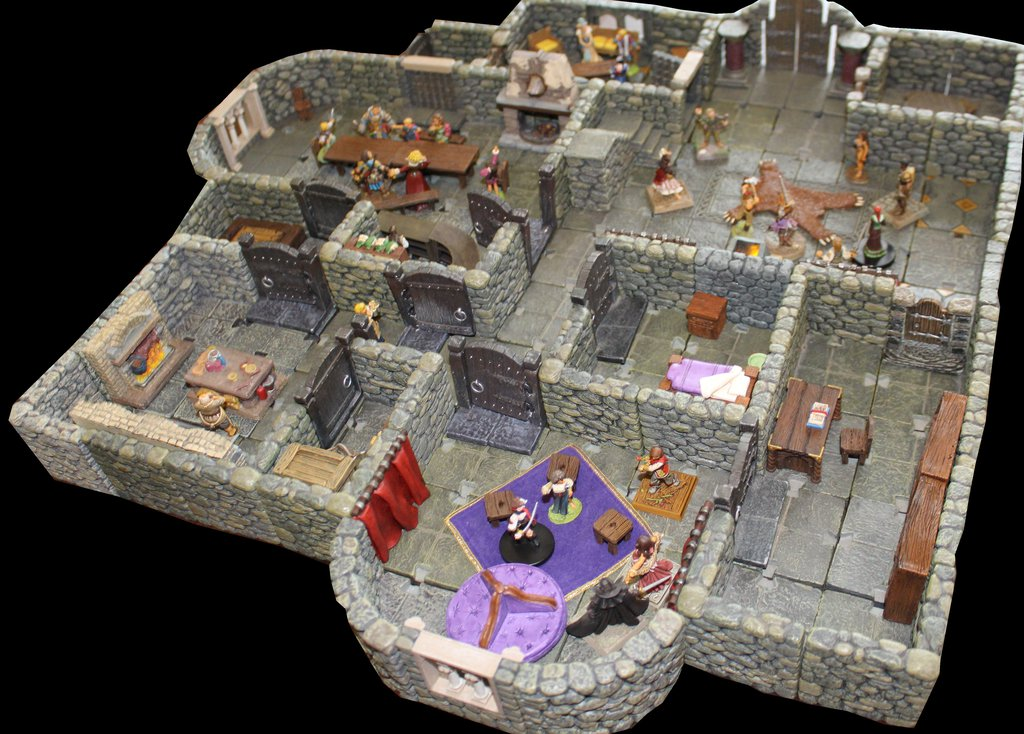
\includegraphics[width=0.39\textwidth]{images/Carowyn-villa-486295633.jpg}
	\caption{Carowyn villa}
	\label{fig:Carowyn-villa-486295633}
\end{figure}

In the front sitting room the companions reconnect with Aaron Endrin, the eldest son of Marcus Endrin, the commander of the Sable Company. Aaron has started his training to become a Sable marine himself, after serving his father as a squire for many years. This role is now being observed by his smaller brother, Jonas, who is here as well. Quint remembers seeing Aaron with Marguerite Jeggare at the grand feast in her family's museum three weeks ago, so he informs if Korvosa's most beautiful girl is here as well. Aaron tells him she won't be attending parties any time soon, as she has joined the queen's guard to serve as one of the Grey Maidens. Quint is quite surprised to hear that, but Aaron explains that he understands the call of military duty. Despite her beauty Marguerite is not an air-headed puppet, but a self-confident and principled young lady who is allowed to make her own choices in life. Christina Leroung disapproves of Marguerite's "dumb" decision. She can understand Aaron's ambition to join the Sable Company, as he was born to become their next commander, but she cannot get why someone from a noble family would chose to play the part of an anonymous soldier, certainly not if she has Marguerite's looks. That girl can get any man she wants, so why she prefers to waste her time chasing windmills is beyond Christina. While the conversation is on the topic of the Grey Maidens, Quint also asks Aaron if he knows where all those new soldiers suddenly came from. Aaron confirms that one ship was registered coming from Cheliax with over a hundred Maiden recruits. Neither the Leroungs nor the Endrins have any sick family members at the moment, although they do realize the threat: diseases do not stop at a nobleman's door.\\

In the dining hall the companions come across even more guests. Verana Ornelos is trying her best to hide her average features by dressing up as a hot succubus, succeeding only partially at the job. Her younger sister Julia possesses a lot more natural grace and looks stunning as a fairy princess. The cute little noble lacks her family's knack for magic, however, so she will be one of the few Ornelos children not pursuing a career in spell-weaving. Her sister Verana, on the other hand, will shortly start her Acadamae education. Belinda Zenderholm takes some time to get to know the companions better. She has heard many good things about them from her mother, high judge Zenobia. She cautions Sjo not to encourage Amin Jalento to drink too much. He is rumored to have got really drunk at the Riverwind Festival three days ago, spoiling what is left of his reputation and his family's good name by whoring and drinking in Eel's End. He is already quite inebriated and shows no signs of slowing down. He wants to share a drink with the men who saved him from half a dozen hot-tempered dockworkers during the riots. He is also glad his father, the "respectable" captain, is not here to rebuke him some more, as he is prone to do, preferably in public. Another person in this room is Perishial Kalissreavil, the half-elven ambassador of the Mierani Elves. He totally lives up to his reputation of womanizer by flirting with Julia Ornelos. Before long he smooth talks her into following him upstairs.\\

The companions meet their closest friends among the city's nobles in the music room. Aisha Leroung, the star of the Saint Alika opera, makes for a sexy vampire tonight. She immediately clings to Quint's arm and wants to know what he's been up to. She has not started a new project herself yet, but she hopes the Marble Dome's director Touran Palastus comes up with something soon. Flamboyant Xerxes Jeggare has chosen to come as Blackjack and feels inspired to play some music with Sjo, Quint and Puk. He takes a seat behind the harpsichord and starts a little session that draws more guest to the back room. His sister Maud is as fine company as ever, joking and laughing in her pretty peacock dress. Sjo strikes up a conversation with Sara Bromathan, who is dressed up as a chaste version of Sarenrae. Like her father she envisions a career serving the sun goddess. She wonders about the source of Sjo's strange divine powers, as she knows from her father that Sjo served as an acolyte to Sarenrae for some time, but then dropped out. Sjo explains that his powers come to him naturally; he has a special talent for fire magic, which puzzles Sara even more. She thinks it might have been wiser to pursue the same path as Verana Ornelos and train as a wizard, but Sjo figures that his powers are more like those of the Shoanti shamans.(Although Sjo is officially an "oracle", that name does not really fit the bill, so if we call him anything at all, we prefer to use the term "shaman", which has absolutely nothing to do with the new shaman class.) Quint remembers why he and his friends came here, to secretly watch over the guests tonight, so he invites everyone back into the main hall, trying to get as many people together as possible. He cannot avoid that some invitees wander off into the dining room to get something at the bar, but with the open door between the two spaces, he can keep tabs on the people in there as well. While the pleasantries of the evening further unfold, the fire in the hearth suddenly flickers and dies out. The candles in the great chandelier follow one second later, plummeting the room in darkness and startling some of the girls. Sjo, who was standing next to fireplace, has no trouble seeing in the dark. His vision might be limited, but it is also more powerful at short distance, allowing him the gift of darkvision. Realizing that he is probably the only one in the room who can see now, a slight grin slips over his face as he reaches for the wood in the hearth. He sends a {\itshape touch of flame} through his fingers to relight the firewood, but is surprised to see a shadowy creature crawling down from the chimney, just inches from his face. The sighs of surprise from the girls turn to screams of terror now. How could Sjo have missed that thing in the dark? Unless the shadow did not show up in his darkvision ... that must be it! With the fire still licking his fingers, Sjo makes for the creature, but the flames do not seem to hurt it. With his other hand the Shoanti pushes back Sara Bromathan, trying to move her out of harm's way. As the fire on his hand dies out again, the room sinks back into darkness and the creature disappears in the black once more. Balian draws his blade and Puk unsheathes his silver blade, both of them standing ready to react. Then Quint casts a  {\itshape light} spell on one of his devil's horns. Although the brightness of his light seems to suffer from the presence of the shadow, \hyperref[fig:Carowyn-villa-shadow-attack-486296086]{ it does reveal that the creature has already flown out of the fireplace and wrapped its dark tendrils around the servant girl } . The frozen look of death stares from her eyes, as she slips to the floor. \\

\begin{figure}[h]
	\centering
	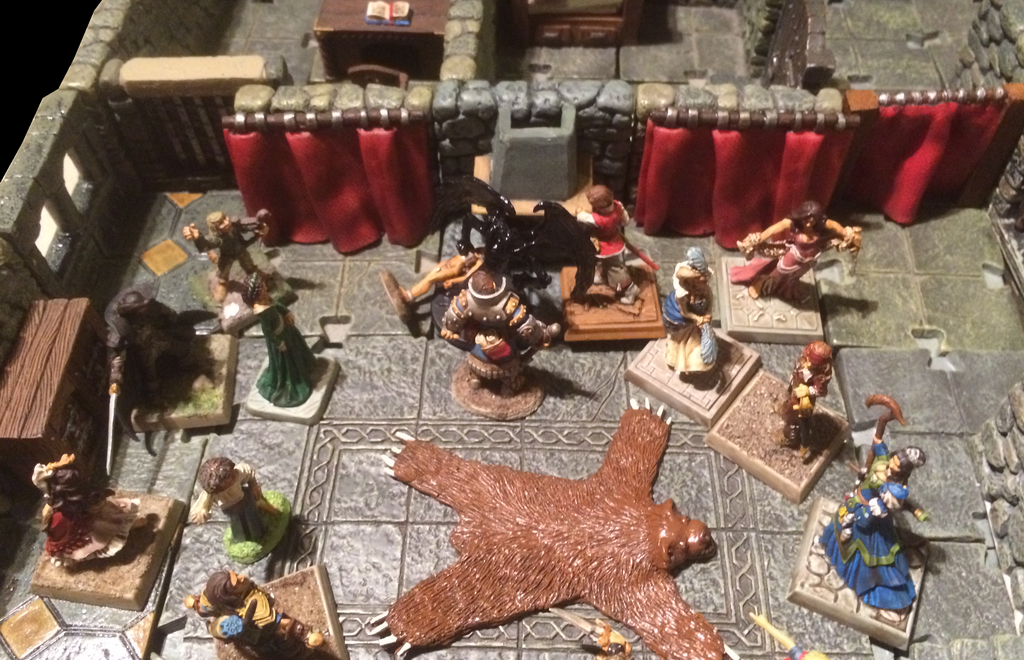
\includegraphics[width=0.39\textwidth]{images/Carowyn-villa-shadow-attack-486296086.jpg}
	\caption{Carowyn villa shadow attack}
	\label{fig:Carowyn-villa-shadow-attack-486296086}
\end{figure}



	%!TEX root = ../crimson_throne_book_main.tex
% 2014-10-18
Panic slips through the crowd in the great hall of the Carowyn Manor. The dark creature that has just crawled from the chimney looms before Sjo and Quint, who realize that almost all of the invitees to this party have been gathered in this one room. The ease with which this lightless threat took down its first victim could very well be the preface to a bloodbath. Fortunately the creature's own tactics prove helpful in getting the noble guests to safety. Weaving its inky magic the shadow blasts out an aura of fear that strikes terror in the hearts of half the people in the room. Overcome by mortal dread Balian makes for the front door and pushes it open, freeing the way for the other guests to flee the scene, even those who have not been affected by the creature's fearful magic. Sjo is also among the unfortunates who are panicked initially, but he recovers even before he makes it out into the streets. Quint, Puk, Xerxes Jeggare and Christina Leroung are the only ones who stand their ground. Quint engages the shadow, taking on a defensive stance, while Christina shouts out that this enemy is extremely hard to hit: you need magic weapons made of cold iron or {\itshape force} magic to hurt it, and even then its incorporeal state and many protection will be an obstacle. She immediately proves her point by sending two magic missiles at the creature that do not penetrate its magic resistance. Puk's first swing also gets lost in thin air. The shadow rewards three of his four remaining adversaries for their bravery by engulfing them in an explosion of green and yellow flames. Not recognizing the magic for what it really is, an illusionary shadow version of a {\itshape fireball} , they are hit to the spell's full effect. Puk relies on his roguish adeptness at avoiding similar magical explosions and evades to lick of the burning tongues altogether, but Quint and Christina are not so lucky and get seriously burnt. Although he is badly damaged, the bard is still on his feet. The fierce daughter of House Leroung does not have enough vitality to survive the blast though and goes down in a smoking heap. Xerxes, who was in the other corner of the room, did not get caught in the burst of yellow and green fire. His mundane rapier will be of no good against this foe, so he rushes to Christina's side to make sure she is still alive. Another ally appears at the top of the stairs, Perishial Kalissreavil, the elven ambassador. He also recognizes this creature for what it is and throws his dagger to the ground: "Take it, it is made of cold iron", he shouts as he fires two magic missiles from his fingers as well. This time the  {\itshape force} arrows penetrate the creature's defenses, delivering some real damage at last. While Quint retreats to administer some much needed healing to his own wounds, Sjo turns around and charges the shadow, using his new dwarven mace. The cold iron from which it was forged proves its worth as the Shoanti tears away some of the threatening shady curls. Puk picks up the elf's dagger, but his feeble swing hardly hurts the opponent. With Balian running wild in the street and Puk being able to only inflict the tiniest amounts of damage, Sjo is the only one who stands some chance at beating back this shadow. His full plate armor provides no protection whatsoever against the incorporeal claws of his enemy, making him an easy target. The creature tears at the Shoanti as if he were naked. Puk finds that his nimbleness provides more protection, but is hit nonetheless and suffers the sting of the cold tendrils. Perishial throws a healing potion down Christina's throat, saving her from death's embrace and pushes the girl into Xerxes' arms, who carries her outside. Quint rejoins the fight and bolsters Puk's fighting prowess with {\itshape heroism} , while the halfling finally manages to slip into a flanking position. His hopes of delivering some serious damage now with his sneak attack prove futile as he finds no weak spot to hit. So he continues picking away at the shade's life force one smoky sliver at a time. Sjo fares better, even though half of each smash is also lost to the air and his blows are answers by smoky claws that totally ignore his mighty plate. At this rate he will never outlast his opponent, so Quint helps out by healing his friend, more or less keeping pace with the damage that is being delivered. Perishial casts his last two {\itshape magic missiles} and shouts he is out, stepping into the next room. A moment later Christina Leroung reappears in the front door. She still looks very weak - she was probably just nursed back to consciousness with some potions - but her sorcerer powers allow her to throw more magic  {\itshape force} missiles at the shadow. Despite the small amounts of damage that everyone is inflicting, the combined efforts of the defenders are slowly wearing down the dark outsider. Somewhere out in the street, already a block away from the manor, Balian snaps out of his panic and stops fleeing. He glares up at the moon, deciding he doesn't like it so much - don't ask - With Quint's healing now balancing out the shadow's strokes, Sjo, Puk and Christina gain the upper hand. The Leroung sorceress blasts two more {\itshape magic missiles} into the swirl of black coils and Sjo calls out to Sarenrae, begging the sun goddess to aid him in defeating the darkness. He hits the shadow twice in rapid succession, ripping the final shred of shade apart. What happens afterwards is a bit of a blur to the Shoanti. His head is still light from the rush of the fight and the drinks that Puk and Quint pour their friends to recover from the excitement. He notices that Cedrik Carowyn returns with a patrol of Korvosan Guards in his wake. Fortunately Xerxes offers to talk to the captain, freeing the companions from the task of making a report. Puk also discovers some kind of rune on the inside of the chimney breast. Whatever this thing was, it was summoned by powerful magic through this magic mark. Since the party is obviously over, the companions head back home again for a good night of sleep.\\



	%!TEX root = ../crimson_throne_book_main.tex
% 2014-10-18
\section{26 Sarenith 4708}

Mouse has a good night and is doing a bit better the next morning. The companions decide to go to the temple of Sarenrae to buy a new wand of {\itshape cure light wounds} . On the way over there they come across an old man in rags who is hanging from a pole. His hands have been tied together above his head and his back is badly scarred from a whipping. The wounds suggest that the lashes were delivered last night. A woman in the streets says that his name is Lombard. He sweeps the streets and makes some extra money selling rats for food to the poor. He was punished by a mob of citizens yesterday for trying to sell diseased rats. The companions cut him loose, heal him a bit and send him on his way, warning him not to pull his stupid stunts again. The seriousness of the plague also becomes clear when a mourning family carries out a heavy body bag and lays it down in front of their house. The city's body carters will be transporting more than just dead rats today. Ezekiel Sollux, the highpriest of the temple of Sarenrae, is glad to see Sjo. He informs his former acolyte that the situation is very bad. The temple has already been converted to an improvised hospital, but the scale of the disease is making it impossible to care for all the sick. He sends out his priests to make as many house calls as possible, transporting only the worst cases to the church. There is some magic available, but that is quickly spent, so the priests have to rely on their mundane training in the arts of healing instead. Sollux asks Sjo to help out a bit and the Shoanti agrees immediately, as does Balian.\\

Meanwhile Quint and Puk pay Cressida Kroft a visit. The Field Marshal gets a full report of what transpired in the Carowyn Manor last night. Quint also reveals that they were warned of danger by the Vudran rabble-rouser Selena. She claimed that the queen is responsible for whatever evil was planned at the party. Kroft can only conclude that this Vudran lady has to be brought in as soon as possible. If she was not responsible for planting the shadow at the party herself, she must at least have more information on who did. Kroft also feels unhappy about the manipulative ways of the dark-skinned woman, whatever her schemes are, they always lead to trouble, so she must be stopped. The Field Marshal also has some news. The queen has summoned doctors from Cheliax to help fight the plague. They will arrive here today through teleportation and Kroft will have to employ her troops to assist these healers as they go into the city. She actually expects them to arrive any moment.\\

Sjo quickly swings by the temple of Shelyn to see his girlfriend, priestess Larella Semyr, but he only finds closed doors. He meets up with his friends and as they head back to the Citadel to see the queen's new doctors for themselves, he ponders on the time when he, Balian and Quint participated in the Pied Piper play while they were still kids. He explains to Puk that they performed the play with real rats on stage. An old woman was hiding underneath the boards, controlling the rodents. Although they were forbidden from doing so, the boys sneaked a peek at the lady while the play was in full swing. That is when they saw her for what she really was, a wererat! Alan, the kind leader of the Varisian theater troupe, told them afterwards that the lady could indeed transform into a rat, but that she was 'one of the good ones' who could do that. Meep Gildenglare still lives in the city; she owns a seamstress shop called {\itshape The Gilded Needle} in North Point on Burnt Bridge Boulevard. Maybe she can shed some light on the rats and their disease. 

	%!TEX root = ../crimson_throne_book_main.tex
% 2014-10-18
When the companions get back to Citadel Volshyenek the Chelish guests have already arrived. They are in Kroft's office, so the heroes have to wait in the courtyard, where more and more soldiers are arriving. The Field Marshal has apparently ordered all troops to gather here for a big announcement. Some Gray Maidens are there as well and stand guard at the doors of the main building. When Quint asks them something, he can tell from their Chelish accent that these must be some of the Maidens who came from the old country, Cheliax. Grau Soldado joins his friends in the crowd and tells them  that his niece Brienna had a bad night again. He doesn't know anything about these doctors, but he suspects that their magical healing capacities - if any - will be limited, so they will mostly have to rely on mundane healing skills. Not all civilians are as lucky as his niece, who can also benefit from Sjo's magic to keep her strength up. The look in Grau's eyes expresses a gratitude that words could never encompass.\\

It takes over an hour before Cressida Kroft finally steps out. At her side is a middle-aged gentleman in a simple black overcoat with streaks of white gracing the sides of his short dark hair. He has a soft, concerned look in his eyes and tightly grasps a heavy doctor's case. They are followed by a more ominous looking group: men wearing cowled robes of oily-looking leather, supple gloves and wide, black hats. Their faces hide behind dark-goggled masks tapering to a pointed beak. Kroft climbs a weathered wooden platform and orders her troops to silence. She introduces the man at her side as Doctor Dave Saulus, the leader of the queen's physicians. The guards will have to escort these doctors in their royal duties, wherever they may take them. They will go into the city to help the sick, but if they want to get a grip on this disease, people will have to cooperate and do what the doctors order them to do!\\

Then Kroft's tone grows grimmer: "There is something else ... you are to consider orders from any of the queen's Gray Maidens to be as binding as any superior officer in the Korvosan Guard." A murmur of protest rises up from the dozens of red-and-gold-armored guards in the courtyard, but Kroft commands them to be quiet. "You are guardsmen of Korvosa, you have a duty to the citizens of this great city. These are dire times and our people need you and they certainly need these healers. You will do as commanded! Now, all patrol leaders to me for your assignments!" Quint makes his way through the soldiers and approaches Doctor Saulus. He offers is assistance in escorting the doctor himself, but the kind man replies that his job consists of coordinating his physicians work, so we won't be needing a personal escort. He does thank Quint for his kind offer, though, and tells him that he might call on him if the need arises.\\

When the patrol leaders have been given their orders, they take their men and leave the citadel with two of the new doctors in tow. The companions also depart, heading to Trail's End to see Grau's niece Brienna. As they travel through the streets of East Shore, a gaunt man with only one eye preaches to them that this plague is the wrath of Urgathoa, the goddess of disease, who is displeased that she has not been given her own spot in the Pantheon of the Many, Korvosa's temple to seventeen different gods, spread out over seventeen small shrines in a huge building in South Point. The Pallid Princess is not among these seventeen, which obviously vexes her. The old man claims that Urgathoa will not stop until every house has lost someone to the plague! The companions ignore the mad man's rambling and focus on aiding sick little Brienna instead. Her mother has already informed two of her former employers that she will be leaving, there is one more person to go before she is free to work at the companions' villa instead. Of course, that will have to wait until her daughter gets better, Tayce says. Sjo and Balian take their time to give the girl the necessary care. When they are finally done, they want to drop by Meep Gildenglare, the wererat seamstress, to see if she can offer any insight or help. On their way over there they notice new posters all over town:\\

 {\itshape "By Decree of Her Royal Majesty, the Radiant Queen Ileosa I, all citizens and members of the Korvosan Guard are to aid and admit the newly established Queen's Physicians in this time of urgency. These royal agents will extend healing to the sick and organize defense against the spreading affliction. They are to be allowed access to any home or building they deem necessary in the course of their duties. All those suffering from disease or disorder are to submit themselves to the Physicians for treatment. To aid in the duties of the Queen's Physicians, know that the order of the Gray Maidens has been established to provide military support as needed. The Maidens answer directly to the Crimson Throne, and will be called upon as necessary to augment and strengthen the peace where simple city guards will not suffice. Impeding or distracting the duties of the Queen's Physicians or the Gray Maidens is punishable by imprisonment. Impersonating one of the Queen's Physicians is punishable by death. Knowingly harboring or hiding the infected is punishable by death. Purposefully spreading the plague is punishable by torture, then death. The Queen's Physicians will be making rounds of every city district henceforth until Her Majesty deems this misfortune abated."}  Meep's {\itshape Gilded Needle} is a cute little shop along Burnt Bridge Boulevard. Meep is still the same kind old lady the companions met five years ago, though she doesn't immediately recognize her visitors. Quint reminds her of the play and refers to her 'power' over the rats. He wonders if she would be able to talk to the animals to find out more. She claims to be very worried about the rats dying recently, as she has four tame rats running around her shop whom she loves very much. She fears for their safety and has decided to keep them indoors for the time being. She confirms that she can exert some influence over them and their kin, but the rodents only possess animal intelligence, so they cannot speak, not even in a secret rat language, Meep smiles. "I can only get them to understand some basic, commands", she continues, "pretty much like you can with your dog. I fear that my aid in fighting this plague will be limited to laying low and hoping that the disease skips my door. I'm sorry I cannot be of more help." 

	%!TEX root = ../crimson_throne_book_main.tex
% 2014-10-29
The PCs have been level five for a few sessions. Here are the stats.\\

BALIAN, CG Male Human ranger 5 (urban ranger)        {\itshape masterwork greatsword} (two handed) +10 ((two handed) 2d6+6/19-20)   {\itshape masterwork dagger} +10 (1d4+4/19-20)   {\itshape masterwork dagger} (thrown) +9 (1d4+4/19-20)   {\itshape masterwork longbow (composite/strength rating+4)} +9 (1d8+4/x3)     {\itshape lead blades, longstrider}        Favored Community Korvosa (Ex)  Favored Enemy (Human +4, Undead +2) (Ex)  Trapfinding (Ex) Trained actor  Child of the Streets  Reactionary Spyder, dog companion level 5, N Medium animal           ---\\

PUK, CG Male Halfling rogue 5 (swashbuckler)        {\itshape silver short sword +2} +10 (1d4+2/19-20) and  {\itshape masterwork short sword} +9 (1d4/19-20)         \section{Sneak Attack (Ex)}

Fast-Talker  Personal Addiction ---\\

Quintilian, CG Male Human bard 5 (court bard)        {\itshape short sword +1 of frost} +6 (1d6+3+1d6/19-20)   {\itshape longsword} +5 (1d8+2/19-20)   {\itshape masterwork whip} +6 (1d3+2)   {\itshape sap +5} (1d6+2)   {\itshape shortbow} +5 (1d6/x3)     {\itshape cacophonous call, gallant inspiration, heroism}    {\itshape cure light wounds, innocence, memory lapse, sleep, timely inspiration, touch of gracelessness}    {\itshape detect magic, ghost sound, light , lullaby, mage hand, message, open/close, prestidigitation, read magic}      Bardic Performance  Versatile Performance (Comedy) (Ex)  Countersong (Su)  Distraction (Su)  Fascinate (Su)  Heraldic Expertise (Ex)  Satire  Mockery (Su) Trained actor  Fast-Talker  Child of the Street ---\\

SHAOBAN (SJO), LN Male Human oracle 5                Clouded Vision  Flame Mysteries  Touch of Flame (Su)   Molten Skin (Ex) Trained actor  Child of the Streets  Ease of Faith 

	%!TEX root = ../crimson_throne_book_main.tex
% 2014-11-01
Evening has already started when the companions leave Meep Gildenglare's shop. Since they haven't eaten anything yet, they head to Eel's End for a quick meal and some entertainment. Sjo swings by Shelyn's temple first, to see if Larella is there now and when he finds her there he asks her to join him. He is a bit embarrassed when one of the girls of pleasure waves at him while he leads his date across the docks of Eel's End. It is the redheaded girl who helped him lose his virginity.\\

The boats of Eel's End are open for business as usual and there is little sign of the plague here, although there are considerably less visitors. Quint spends some time in the brothel in the arms of his favorite, Yuuna, feeling even more enticed by her Vudran heritage than before since that other dark skinned beauty Selena has been eluding him. According to Balian the two girls look quite alike, although Selena possesses a more natural flair. Quint also inquires about the ship that sunk in the harbor. Yuuna didn't see it herself, but some of her colleagues witnessed the burning ship go down further up the river a few nights ago. News of the queen's physicians hasn't reached the House of Clouds yet. Yuuna explains that Old Korvosa is usually the last district to deserve the palace's attention, so it doesn't surprise her that the doctors didn't make it here yet.\\

When our friends finally return home, Korwick tells them that Vencarlo Orisini came by earlier today. He was in the neighborhood as he had to go the temple of Pharasma. Someone died ... although Korwick does not remember who exactly. Anyway, master Orisini had to be in the temple about this guy's funeral, so he decided to stop by, but he went home when he found out the companions were not there, without leaving a message.\\

\section{27 Sarenith 4708}

Sjo feels a bit under the weather that morning and Mouse is doing worse as well. The big man uses his {\itshape lesser restoration} spell to take away the worst of the sickness's effects. He also pays another visit to young Brienna in Trail's End and cares for her too. Then he retires home to his bed to get some rest. Meanwhile his friends go to Vencarlo Orisini. The fencing master's academy is closed today. Quint immediately notices that Vencarlo didn't get much sleep last night. He also smells alcohol on his breath. Vencarlo explains that his loyal servant Raldo passed away yesterday. He got sick with the plague a few days ago and, as he was already advanced in years, quickly succumbed to its devastating effects. When Vencarlo Orisini went to the temple of Pharasma to make arrangements for his servant's burial, he heard that 37 citizens had died already and a lot more people were sick. The mysterious illness that had just popped out of nowhere had taken a choking hold on the city in just a few days time. Old Korvosa and North Point were hit the hardest.\\

Vencarlo worries about the feeble attempts of the city's churches to fight the disease. He feels that they could work much more efficiently if they were to coordinate their efforts. The church of Sarenrae has good intentions, but seems to be overrun, Pharasma is dedicating all her efforts to burying the dead, while Abadar's Bank has even closed its doors to the public, letting in only those who can pay. If the companions want to do something for the city, they should see to it that the temples get organized. Quint and Puk agree wholeheartedly and decide to take action right away.\\

They go to the temple of Sarenrae first, figuring that they'd better start with the one who is most likely to accept. It will be easier to convince the harder cases if you can say that other churches have already consented. Ezekiel Sollux, the highpriest of Sarenrae, is tending to the sick himself when the companions walk into the improvised hospital that his temple has become. When Quint explains his idea of coordinating the churches' efforts better to allow the priests to administer the most healing possible, Sollux agrees. Although he is doing everything within his power to help the sick, he has no clear overview of what his priests are doing, of who they are helping and who not. If there were more people to lend a hand with the simple stuff, like feeding the patients or changing their sheets, the clergy would be free to focus on providing care. Quint asks him who in his temple would be a good representative, someone who can supervise the work within the church and consult with the other faiths, Sollux has just the man for the job: Lord Valdur Bromathan. Although the head of House Bromathan possesses some priestly magic, his powers are limited. He is a good organizer, though, and his age and title give him the necessary authority to carry out the job.\\

The next destination is the church of Pharasma. On the way over there Balian has to shake off a woman who grabs him by the shoulder, screaming that this disease is all an evil wererat plot. The cathedral in the Gray district is also flooded with people, although not many of them look especially sick. Most of the visitors are mourners who have come to make arrangements for the deceased. Archbishop Keppira d'Bear is ashamed to admit that she and many of her priests make it through the day without even spending all the magical healing they are capable of, simple because their work with the dead keeps them so busy. She even has priests digging graves since some of her usual grave diggers have fallen ill or have bolted as they fear getting infected by handling the corpses. As a priest of Pharasma d'Bear does not consider her task of burying the victims of the plague mundane or menial, but she does recognize that healing potential is being wasted. If there were people around to help with the administration, preparing the dead for interment or for digging the graves, that would definitely open up time for her clergy to focus on healing people and saving lives. She suggests making brother Aldrick the church's representative. His high position in the church's ranks earns him a great deal of respect, both inside and outside the cathedral, but being a paladin, his powers to heal are more limited than his priest colleagues.\\



	%!TEX root = ../crimson_throne_book_main.tex
% 2014-11-01
Keppira d'Bear also has a request: yesterday brother Cedrik did not return to his cell to sleep. No one knows where he is, but as the temple is swamped, there is no time to look for him. D'Bear asks the companions to help locate the missing man. Sister Fryda shows the companions to Cedrik's bedroom, but nothing seems to be out of the ordinary. Cedrik's prayer book is still by his bed. He would never leave it behind, Fryda claims. She also adds that Cedrik is a as devout as they get, so he would never just run away or something. Since he came here at the age of twelve, he has never even set foot outside of the Gray district. He is also a very diligent man, never late and very precise in everything he does, which is why he is the church's accountant. He mostly works in the office, keeping the books, but yesterday he was tasked to help out in the mortuary.\\

By the way, this sidetrek adventure is based on a cute little Quint and Puk also have a quick look around Cedrik's office. His desk is piled with dozens of documents that still need processing, listing names and relevant data about all those who have died. Under the pile is a book that has been opened to a page detailing Pharasma's holy chalice. When sister Fryda sees the drawing, she claims that the cup is in the very mortuary where brother Cedrik was sent to yesterday. Our friends decide to pick up Sjo first before continuing their investigation. The Shoanti has been in bed for the last two hours, vainly trying to catch some extra sleep, though frustration made it feel like it lasted much longer. It takes some convincing, but fearing more endless hours in bed, Sjo gives in and joins the quest for Cedrik.\\

Fryda leads the companions to a smaller building behind the cathedral, the mortuary. She takes them through a small chapel with beautiful stained glass windows to the preparation room in the back, where the chalice should be. There are two stone tables, each the resting place of a dead body, covered in a white sheet. A small stone altar stands in the corner, it has nice stone carvings in the sides, depicting Pharasma's Boneyard. The altar holds nothing, but a distinct circular discoloration in the stone suggests that something round has been on top for many years. The chalice, however, is missing, Fryda notices. Balian examines the small altar more closely and finds recent scratches on the floor which indicate that the stone altar can swivel forward. A skull in the boneyard bas-relief on the side of the stone block can click, propelling the altar away from the back wall and revealing a hole in the ground underneath. Fryda screams in surprise, she didn't know that the altar could do that. Quint conjures up some light to shine down the opening: there is a 15 foot drop into a small natural cavern below which wafts forth a foul odor of earth and mold.\\

Puk retrieves a rope from his pack and ties it to the stone table. Sjo is the first to go down, trusting his darkvision to warn him of any danger. He ends up in a small cave with two exits: a rough archway leads into a larger chamber in front of him, while a tunnel slips off to the right. Still, it is the chamber that draws his attention. The light falling in from above reflects in thousands of tiny specks of light. The entire frame of the door and all the walls, floor and ceiling of the chamber beyond are covered in a silver dust coating. The step of the archway is also inscribed with silver runes. When his friends have joined him Sjo uses a {\itshape read magic} to decipher the mystical writing: a powerful spell meant to block the passage of undead. Quint detects that the magic was broken very recently. The companions step into the rectangular chamber, which was obviously manmade, unlike the cave and tunnel behind them. The air in the room is stale. The silvery floor is covered in dry brown dust and holds the heavily gnawed bones of two rats. Despite the fact that the bones have been picked clean completely and most of them have been chewed to pieces, Balian can tell that they are recent, very recent even. No more than a few days ago these rodents must have been very much alive.\\

Leaving the chamber behind them, Puk and Balian lead the way down the tunnel to a small cave that seems to be little more than a deviation point. A slender stalagmite rises floor to ceiling in the far end of the room with a steady stream of water droplets running down its side. A pool has collected at the bottom, trickling away to the left in a shallow stream of water down another tunnel. A second tunnel winds away to the right. As the floor is quite uneven and wet, Quint pulls out his wand of {\itshape feather step} to grant everyone more stability in difficult terrain. Sjo scratches a cross in the wall, marking the way out. Ignoring the tunnel with the trickling water the companions head the other way through the winding tunnel that leads into a vast cavern. The ceiling does not extend much higher than the top of the tunnel, but the ground drop down in a number of stone tiers to a treacherous floor. A narrow chasm cuts across the middle of the cave from left to right, roughly cutting the room in half. While Sjo makes his way down, Balian shouts out a word of warning. Something is moving in the shadows along the wall. Suddenly a foul creature bursts from the dark; it is clearly humanoid in shape, although its nails and teeth look unnaturally long. Its pallid grey flesh stretches tightly over its starved frame. Quint jumps to his partner's aid and pierces the creature's dried out innards with his icy short sword. The undead hits the bard in return with its sharp claws. Two more ghasts break from the darkness up ahead, hungry for fresh meat. One of them sinks its pointed teeth in Balian's shoulder, but the other misses the nimble halfling by a long shot. The undead fight and bite fiercely, drawing some blood from the heroes, but they go down quite easily. In a few seconds the brawl is over. Puk discovers the remnants of some kind of uniform on the ghasts' upper body, on which Quint can barely make out the former shield of Cheliax. It dates back to the days of the settlers, three centuries ago, that Chelish soldiers walked Korvosan soil. Whoever these undead were in real life, they must have been here a long time.\\

This side of the complex ends in another large, irregular cavern, where two more ghasts attack the companions. The walking corpses are easily defeated. One more undead has stumbled into a pit in the floor, unable to get out. Balian simply finishes it off with his bow. There are more rat cadavers on the floor, but this time the remains have been only half eaten. A number of small holes dot the north wall: tiny tunnels through which diseased rats made their way into the complex. Balian figures that the disease forced the rodents to retreat deep into the ground and that the rats unwittingly provided the famished ghasts with a food source for the first time in centuries.\\



	%!TEX root = ../crimson_throne_book_main.tex
% 2014-11-02
In the absence of other former regular posters, please let me just tell you that I am still eagerly following this journal. As I have not played the Adventure Path myself, sometimes it is a bit hard to keep track of all the characters poppin up now and then but I guess the interaction with so many various NPCs is just what makes this AP stand out from the others and has arguably turned it into the most popular of all APs. Kudos to you as the DM for fleshing them out even more and establishing closer connections to the PCs as this makes the setting come so much more alive. Looking forward to the next entry!\\



	%!TEX root = ../crimson_throne_book_main.tex
% 2014-11-02
I'm still here, I'm just lurking and eagerly reading/awating future installments.\\



	%!TEX root = ../crimson_throne_book_main.tex
% 2014-11-08
Happy to hear that you're still reading and you still like the story.\\

It is one of the things I find most difficult when reading other journals - remembering who all the characters and NPCs are - which is why I hope the pictures help to get an image of the PCs and some of the settings. Still, there are a lot of characters in this story, so yeah, it might get hard sometimes. It certainly helps to be familiar with the AP, because then you can at least tell those NPCs apart (like Kroft, Orisini, Trinia, Tuttle, Ornelos, Arkona, d'Bear ...).\\

I also understand the fact that you do not write a comment every time you read a new entry. I read some other journals myself, and even though I try to leave a note at least once, I do not do so every time - far from it. I only speak up when I have something to say or to ask. Still your little comment was appreciated. I hope you'll enjoy what I have in mind for my group. If things work out as planned, there should be good times for years to come ...\\



	%!TEX root = ../crimson_throne_book_main.tex
% 2014-11-08
I don't like to populate campaign journals with comments too much because I find it can take away from the story of the journal itself. It's like having to pause a movie because two people are talking.\\



	%!TEX root = ../crimson_throne_book_main.tex
% 2014-11-15
With no sign of brother Cedrik in this end of the complex, the companions retrace their steps to the first crossroads chamber with the small pool. Having explored the right side, they now dive into the left tunnel, which slopes down across a hard stone surface. Centuries of water trickling down have worn the steep floor smooth, making it treacherous to navigate.\\

The passage ends at a cavern with a domed ceiling, cramped with stalactites. Several of these hanging formations have grown together with the stalagmites on the ground, making up one colossal pillar. At the foot of this beautiful column a large clear pool has formed. Quint tosses a {\itshape light} stone into the water. It looks quite deep, at least seven feet. A man-shaped shadow rests against the stone pillar below the water line: the calcified remains of a long forgotten man. Two tunnels lead off into the darkness, one just around the corner to the right and another at the far end of the cavern. Reaching the other tunnels is hard without getting wet. Sjo decides to head back to a spot with even footing, where he can take off his plate armor. Meanwhile Puk, Quint and Balian investigate the right corridor. They come across three more ghasts, but they dispose of the undead easily. Balian peppers them with arrows from the back line, while Quint tries to trip them with his whip, giving Puk the opportunity to stab them with ruthless efficiency. The tunnel ends in a stone door at which the undead have obviously been scratching. The left bottom corner of the door is missing, revealing a small room beyond in which some scared rats have taken refuge. So the ghasts were after more rodents to eat! Balian pulls the door open. The room looks manmade and is strewn with the decayed remains of wooden crates. Apart from three diseased rats there is nothing here worth noticing.\\

When they return to the pool cavern, Sjo joins them in nothing but his shirt. Quints digs up a wand with {\itshape mage armor} to boost the healer's defenses a bit. One more tunnel remains, but to reach that, the companions have to cross the water. Balian and Puk manages to keep to the side of the cavern, but Sjo and Quint lose their footing and glide off into the center of the pool. They use this opportunity to examine the skeleton at the foot of the pillar and discover a gold bracelet on his right arm. Before climbing up the final tunnel, Quint weaves a {\itshape prestidigitation} through his fingers to dry everyone's clothes. Puk leads the way into a shadowy cavern. A dark shape jumps forward from an alcove in the opposite wall, splashing water over the halfling and shouting: "Stay back, you fiends! In the name of Pharasma!" It is brother Cedrik, still a bit wet and tired. He has caked blood on his forehead. When the wide-eyed priest understands that the intruders are there to save him, he is overcome with relief and spills the beans on what happened. He was tasked with working in the morgue and he remembered the chalice that was there. Since he had always been told that it possessed certain magical abilities, he wondered whether it might be helpful in fighting the plague. So he looked up some information in his books, but he came up with nothing of real interest. His next best guess would be to examine the cup itself. Upon arriving in the morgue, he went into the backroom to look at the chalice. He was surprised to hear strange sounds coming from below the floor, underneath the stone altar. Trying to pull the heavy block of stone aside, he accidentally pressed the secret button in the bas-relief, triggering the opening mechanism. The altar slid away, making the chalice on top topple and fall down the hole that was revealed underneath. Ashamed at his clumsiness Cedrik jumped into the dark to retrieve the cup, but the drop was deeper than he had estimated, so he hurt his ankle. His arrival in the underground chamber was met by hungry growls and grunts from a host of undead. Before they could reach him, Cedrik snatched up the chalice and ran off into the only available exit. He stumbled down the steep, slippery tunnel into the pool chamber, hitting his head before plunging into the water. As he heard the ghasts coming after him, he quickly climbed out of the pool and hid in the far corner of the cavern, keeping his flask of holy water at the ready. He spent a very scary night there, but fortunately, the undead never came for him.\\

There is one more exit from this final cave: a heavy stone door marked with Shoanti runes. They talk of {\itshape Shemnoata the traitor} , who led the  {\itshape intruders with the long, white knives} into his home camp, resulting in the slaughter of 58 warriors, women and children. Sjo feel uncomfortable disturbing the passage, but Quint and Puk are eager to explore it. Balian pushes at the door, but when it finally gives way, he almost falls down the sinkhole that is beyond, for indeed, the roughly circular cavern has no floor, but rather drops away into the dark. Jutting from the far wall are seven evenly-spaced spears. Mounted at the end of the shafts are jawless human skulls, all turned to face the door. They boom in old Shoanti: "Begone! Let the one who betrayed his brethren rest!" Balian notices that the sinkhole has some kind of alcove about thirty feet down. Puk climbs down a rope and discovers a small secluded compartment in the side of the sinkhole which holds an unadorned stone tomb. Balian and Quint join the halfling and the bard casts {\itshape detect magic} . He sees a slight sheen of magic emanating from beneath the heavy lid. Together the three young men push aside the cover a bit and look upon the leathery face of the body inside. With a low-pitched sigh the corpse opens its eyes and stares back at the adventurers. Balian reacts immediately and plunges his blade in the dead man's face, tearing apart his jaw. Quint and Puk are hindered by the lid that still covers most of the tomb and thus protects the corpse. Then Shemnoata's gaze takes its true effect, confusing both Balian and Puk, making them either hurt themselves or babble incoherently. Quint tries to hold back the undead with  {\itshape cure light wounds} touch attacks, while Sjo quickly makes his way down the rope to help his friends: "You fools, I hate to be the one to say I told you so, but ... I TOLD YOU SO!" Shemnoata throws off the stone lid, making it disappear in the sinkhole, and stands up. By that time Sjo arrives and hits the risen dead hard with his heavy mace. Quint's short sword finishes him off once and for all, simultaneously ending the insanity that has taken hold of Balian and Puk. Quint casts another {\itshape detect magic} , which gets a much brighter reaction now, coming from the corpse's silver belt. With Zellara's aid Sjo identifies it as a  {\itshape belt of physical might} , which enhances both one's strength and stamina. This powerful item is perfect for a swordsman like Balian. Puk remarks that the girdle is of Chelish make, so it probably was the traitor's payment. That would explain why he was buried with it, for none of his brethren would have wanted the cursed item after they'd killed him. With the underground complex completely explored the companions return to the morgue. Sjo and Quint ask Zellara's insight in the mechanism that kept the undead locked in. It seems like the proximity of the chalice acted as some kind of key to seal undead into the silvered room. Now they can finally reconstruct what happened. The diseased rats somehow made their way into the old underground complex and disturbed the undead's slumber by providing them with food for the first time in centuries. The ghasts' loud meal alerted Cedrik, who accidentally managed to open the secret passage and who jumped into the hole to retrieve the fallen chalice. There he saw the undead, not realizing that they were still locked into the silvered room because the chalice was still close-by. The panicked priest grabbed Pharasma's holy cup and ran off, thus removing the 'key' from the holy barrier and breaking its magic. The undead were finally free after three hundred years. Fortunately for the clumsy priest the ghasts were more interested in food and made off after the diseased rats, leaving the chamber where Cedrik had sought refuge in peace.\\



	%!TEX root = ../crimson_throne_book_main.tex
% 2014-11-15
High priestess Keppira d'Bear is pleased to see Cedrik is safe and is sighs when he tell her what happened. She offers the companions her full support in their efforts to fight the plague, provided they get her help for a number of more mundane tasks. She also wishes them luck trying to convince the churches of Abadar and Asmodeus to join the 'medic task force'.\\

The Grand Vault of Abadar is composed of well-kept grey-veined white marble walls with gleaming bronze friezes, all of which radiantly reflect the light of the sun. The structure towers over surrounding buildings and, along with its steep stairs and ramps leading up to the temple's great bronze doors, boasts an aura of divine luxuriance. Today however, the great stairs do not exhume an aura of grandeur, but rather of chaos. Dozens of desperate civilians - mostly of the working class - throng the entry, scarcely being held back by a group of gold-armored guards. Puk sees one man dressed in fine silks pushing through the pock-scarred crowd. To all everyone's dismay, this rich man is allowed inside. The protectors at the gate are heavily pressed by the angered bystanders when Quint speaks out to calm everyone down. He urges the sick to return home, so they can rest and get better instead of tiring themselves here and infected even more fellow citizens while they're at it. He promises them to talk to the Archbanker and work out an arrangement so they can be helped. After the crowd disperses the guards let the companions in.\\

Archbanker Tuttle welcomes his guests and can be convinced that he will serve order and civilization better by joining in an organized effort to fight the plague. Unlike the churches of Pharasma and Sarenrae, he is not looking for extra hands to help out in his temple, on the contrary, he does not want strangers running around his Bank. So he will help, but at another location. He agrees to meet with the representatives of the other churches tomorrow and already feels like he should be the one to be the overall coordinator. If the companions want to appeal to the general public to help, they might just as well ask for donations, which would serve the Bank of Abadar better than 'helping hands'. Despite his willingness to join in the medic force, Tuttle will keep back some spells for his own followers, he says. After all, if they are sick, they deserve to be treated just as much as everyone else!\\

The church of Asmodeus is one of the most magnificent buildings in the city, built from red marble in the shape of a five-pointed star, and situated upon Citadel Crest in the wealthiest ward of the city. The church competes with Abadar for the right to verify and witness oaths and contracts. Since his initial error in judgement - when he sacrifices thirteen maidens to his deity - high priest Ornher Reebs has taken great pains to operate on the right side of the law. Despite this focus on its lawful nature, many Korvosans see the church of Asmodeus as an evil entity in the city and carry a deep mistrust for the infernal religion.\\

Unlike the other temples the church of Asmodeus is not overrun with people. The sturdy bodyguard Mallas summons his master and hangs around to keep an eye on things while his superior talks to the companions. Ornher Reebs is not happy to see Sjo, who attempted a short apprenticeship in the temple, before turning his back on it. To Reebs that kind of cowardly behavior smells like breach of contract. Quint plays the 'pride' card when he says that all the other churches have agreed to help out, so it would be a 'shame' if Asmodeus would not join in. Reebs wants to know how much the Bank of Abadar is being paid for its help and when he learns that the companions plan to raise money through donations, he demands half of the proceeds. He also wants the companions to communicate about his church's involvement in a positive light, so more people in the city might grow to appreciate his faith. He even draws up a contract stipulating the exact lines of his conditions. In return he offers his full array of disease fighting spells, as well as the couple of useful spells that his subordinate Tyresha can cast. He knows that there are only two priest in his church who can cast {\itshape remove disease} , but the weight of one high priest easily overshadows a dozen low level clerics. Reebs is the third most powerful priest in the city, so the companions will need his help. Quint and Sjo realize that the man is right: high priests can ask their god for many  {\itshape remove disease} spells when they fill all their higher level slots with this power as well. Moreover, the chance at success depends on how powerful the caster is, so Reebs would certainly add value to the task force. The negotiators agree and put their signature plus a drop of their blood at the bottom the contract that Ornher Reebs draws up. 

	%!TEX root = ../crimson_throne_book_main.tex
% 2014-11-30
After having procured the cooperation of all the major temples in Korvosa to combat the plague together, Sjo has little difficulty in convincing his girlfriend, Larella of Shelyn, to join in the effort, although her contribution will be very limited. She has only just reached the power to cast {\itshape remove disease} and her chances to fail at getting someone better are still bigger than her chances to succeed. Still, she's more than happy to help. Next the companions want to pay a visit to Dave Saulus, the Chelish doctor who leads the Queen's Physicians. They learn from Cressida Kroft where to find him: he's setting up a hospital in an empty warehouse, just a block away from Zellara's old fortune-teller's shop in the harbor area. Dozens of laborers are getting the building ready; a newly painted sign at the door identifies the place as {\itshape The Hospital of the Blessed Maiden} , a reference to Saint Alika. Doctor Saulus is in an office on the first floor and listens quietly as the young men inform him of their plans to form a medic force by having all Korvosan temples pull their resources. Saulus confirms that the number of diseased people certainly justifies a second hospital in Korvosa and agrees that it is best that both medical centers gear their activities for one another. The companions decide to invite all the parties who are fighting the plague in their own villa the next morning for breakfast. This first meeting will launch the medic force, and hopefully it will go on to lead a life of its own without the heroes' further involvement. Cyril Fordyce, the editor of the Korvosa Herald, even agrees to print a public call for help and funds in his periodical's next issue. Quint says he will get his final text tomorrow, after the meeting in the villa.\\



	%!TEX root = ../crimson_throne_book_main.tex
% 2014-11-30
\section{28 Sarenith 4708}

The next morning Mouse is still feeling ill and Quint, Korwick and Heldrin are a bit under the weather as well. That means that all the kids and both Sjo and Quint have been infected. Only Balian and Puk are still feeling healthy.\\

Soon the guests for the breakfast meeting arrive: Valdur Bromathan of Sarenrae, brother Aldrick of Pharasma, Archbanker Darb Tuttle of Abadar and Ornher Reebs of Asmodeus. These four representatives of Korvosa's most important churches are joined by Doctor Dave Saulus of the Queen's Physicians and Sjo's girlfriend, Larella of Shelyn, who spent the night in the villa for the first time. Sjo welcomes everybody and leaves the guests to come to their own agreement. Darb Tuttle immediately takes charge and the others let him. When it becomes clear that the heroes signed a contract with the highpriest of Asmodeus, promising him 50 % of all the funds raised, there is some discussion, but the medic council finally decides to discuss that matter at a later date. For now they agree to place collection boxes in all the temples and they also decide on a text to be printed in the Herald.\\

When the guests have left, Sjo and Balian see to all the sick in the house. By noon they go to Trail's End to take care of little Brienna as well. The girl still hasn't recovered, although Sjo's healing has kept her relatively well. Brienna's mother Tayce inquires if the companions have already heard of the {\itshape cure} that is supposedly available somewhere in the Heights district. They obviously haven't, but a potential medicine certainly piques their interest, even if - which they suspect - it turns out to be a sham. Some information gathering quickly points them to Lavender's Luxury, a perfume boutique. The shop stands in a row of tightly packed houses in Summoning Street, just south of the Acadamae. The owner is a Chelaxian woman named Vendra Loaggri, who is famous for her avant-garde creations and brazen promotions, like her "Free Imp with every purchase" stunt last year. A long queue of eager Korvosans waits in a line that stretches far around the corner. Several of those waiting bear the obvious blistered symptoms of the plague. A strong man guards the door and eyes every customer that enters closely. A customer leaves the perfumery and immediately applies a greasy ointment on his neck. He refers to it as Lavender's Luxuriant Liniment and claims that he already feels better, even though Sjo notices no changes in the man's red spots and Quint detects no magic. Quint wants to sneak a peek inside, but dreads the thought of having to queue for hours, so he decides to start a new line for those who want to buy perfume instead of the cure. While most queuers throw angry glances at the bard, his fast-talking overwhelms them enough so he can get away with his little scheme. About fifteen minutes later he is inside the shop, where a happy-looking dockworker is giving his unbiased personal testimonial of how the luxuriant liniment cured him of the plague. A woman with clear blue eyes asks Quint what he wants when he reaches the counter. The bard recognizes her as Vendra, Loaggri, the shop's owner. From her he learns that Lavender's Luxuriant Liniment has already been around for a long time, but the merchant only recently became aware of its special plague healing ability when a customer who had used it got better. Quint finds it hard to determine whether the woman is lying of whether she truly believes the ointment works. He ends up buying a bottle of perfume and Puk picks up a dose of the cure, because he wants to have it examined.\\

Back in the street Quint teases Sjo about his new girlfriend, giving the big Shoanti the impression that he is a bit jealous. As the two young men are harrying each other, they suddenly hear a loud scream. A group of people have gathered down the road and Quint can tell that are crowding a woman who is clearly in a state of panic. The frightened girl has blond hair and is dressed in a white sheet with no clothes underneath. Sjo gets the bystanders to give her some space while Quint calms her down. When they ask her for her name, she doesn't know ... she doesn't remember who she is or how she got here! An old lady tells the companions that she noticed the girl staggering down the street in naught but a white sheet, looking disoriented. When she asked the girl if she was okay, she started wailing like a madwoman. Still, she seems to be in fine physical order, very fine even as she looks very attractive. Quint wants to get the poor thing some clothes and convinces the old lady, who lives close by, to sell him a skirt and a blouse. Despite this sober attire the girl looks stunning when she puts on the clothes, especially when they prove to be a bit tight around the chest. Sjo and Quint continue to quiz her to see if she remembers anything. When they talk about Sarenrae, Asmodeus or Abadar, she recalls the names and portfolios of those gods, although she cannot name any godhood spontaneously. They lead her down the neighborhood to try and trigger her memories, but nothing comes back. When Puk mentions food, she realizes she is quite hungry, as are the companions, who haven't had lunch yet.\\

Balian suggests grabbing a bite in {\itshape The Travelling Man} in Old Korvosa. The girl shows table manners while eating her burger, indicating that she is not from the lower classes, although she does not display the elaborate etiquette of the nobility either. The girl is very worried and every question the companions ask her sends her into a state of alarm. Is she a criminal? Or someone who was about to be sacrificed in the temple of Asmodeus? Did she rise from the dead or did she use to be a statue that was turned to flesh? She hasn't got a clue. During the conversation Quint notices some men in the square who are pushing a cart with a dead body. It is not until they have disappeared from view that the bard starts wandering why the body carters were going west instead of east, to make for the bridge south for the Gray District, where all corpses have to be delivered. Still, the pleasant company at his table soon makes him forget his contemplations for more agreeable worries, the pretty girl's lot. Focusing his gaze on her shapely curves, the bard casts a {\itshape detect magic} which reveals a hint of magic on her. Sjo joins in with his own spell and reads a touch of transmutation in the lingering magic. The two men try to get the girl to imitate some of their simple spells, to see if she masters the art of spellcasting. It yields no success, although the girl admits to feeling some familiarity to spell weaving. The companions also experiment with the girl's reflection in the window, but seeing a mirrored version of herself triggers no memories. Finally Sjo proposes naming the girl, since it is hard to talk to someone without a proper name. Balian comes up with a nice suggestion, Madam Nesia, the lady who suffers from Mad Amnesia.\\



	%!TEX root = ../crimson_throne_book_main.tex
% 2014-11-30
Big praise goes to my friend Moonbeam, who introduced Nesia in his {\itshape Curse of the Crimson Throne} journal, which you can find here obviously this thread is forbidden for my own players! 

	%!TEX root = ../crimson_throne_book_main.tex
% 2014-12-06
Puk takes Madam Nesia to the villa while his friends follow up on the body carters who were going in the wrong direction. A vagrant at the side of the road calls out and asks them if they want to buy a cloak of rat skins. Sjo gives the man some silver, but immediately burns the filthy cape. For some extra coin the bum reveals that the carters pass by regularly. "They always disappear down a dark alley over there." The man points out where it is.\\

The high walls of the surrounding buildings throw the awkwardly bent Racker's Alley into constant shadow. The hidden sideway is rich with the stomach-turning stench of rot. Heaped against the wooden back wall, behind an empty cart, rises a pile of dozens of plague victims and hundreds of dead rats. The entry to a door has been left clear: it is the back entrance of a small rundown shop called {\itshape Giotorri's Toys} . The front door and windows have been boarded up, making the place look deserted, but the back door seems to be unlocked. Balian puts his ear against the wood and hears voices inside. The ranger pushes in, surprising two body carters in the shop's backroom. Sjo calls out to them: "In the name of the law, lay down your weapons!" But the fools do not head his words and make for their clubs. While Quint starts mocking them with his {\itshape satire} , Balian jumps forward and whirls his greatsword in a devastating arch, gravely wounding both men. (Double critical hit on a cleave.)  {\itshape burning hands} spells from Sjo and Balian's cleaving blade take them down. One of the carters makes it outside, but Spyder and Quint halt his escape. The final opponent surrenders. In the front room Balian discovers a stain of dried blood, no older than two days. The lone survivor confesses that he and his colleagues were tired of making the many long runs from north to south across the city with the corpse carts. So they started ditching the dead rats and bodies in this shady back alley. They thought no one would mind, but then it turned out that someone still lived in the boarded-up shop next to their perfect little dumping ground. Toymaker Giotorri had locked himself in his shop to keep the plague out, so he obviously wasn't too keen on having the infectious cadavers piling up against his back door. The carters tried giving him money, but when he refused, things got out of hand and they killed the old man. That is why they attacked the companions, because they were trying to hide a crime ...\\

Our friends take the murderer to prison and swing by the university to talk to its professor in alchemy, Sirtane Leroung. They ask her to examine Lavender's Luxuriant Liniment, hoping she can tell them whether the ointment really works. Sirtane seriously doubts it, even at first glance, since the substance can hardly even be called an ointment, looking more like grease. The professor in turn asks her visitors if they have heard of anyone recovering from the disease, or even better, of anyone who is immune. Since she cancelled her classes to avoid the danger of spreading the plague, she has been studying the pestilence, hoping to find a cure. Knowing that people actually recover from it, would be a great support. But the real clue to fighting the deadly malady could come from those who possess a natural resistance to it. The companions promise to ask around and keep her informed. They pay a quick visit to Field Marshal Kroft and the temple of Pharasma to report on the carters' scheme in Racker's Alley, before retiring to the comfort of the villa.\\

Puk has already taken Nesia to the tailor's and she is in the bathroom right now, getting ready for dinner. She may have lost her memory, but she certainly did not forget how the dress up: she looks absolutely stunning. Sjo offers the lost girl his bedroom and spends the night at Larella's.\\

\section{29 Sarenith 4708}

The children are still sick and Quint is feeling worse as well. Sjo on the other hand feels great, it looks like his body has fought off the infection. Balian is still as healthy as a fish and Nesia is in excellent physical shape too, but her mental problems persist as she still has no recollection of who she is. Balian and Sjo spend a couple of hours tending to the sick, including their daily visit to little Brienna. After lunch they talk to Sirtane Leroung again. The alchemy professor confirms her suspicions: Lavender's Luxuriant Liniment is nothing more than animal grease, mixed with weeds and some cheap perfume to make it smell less revolting. It has no healing properties whatsoever, apart from the potential placebo effect.\\

The companions report the matter to Field Marshal Kroft, but she lacks the manpower to do anything about Lavender's Luxury herself. She implores the four friends to attend to the case personally. She trusts them to handle the matter in whatever way necessary, but they have to close the shop, because all those people in the queue infect each other. This place offers no cure, on the contrary, it is a serious health hazard.\\



	%!TEX root = ../crimson_throne_book_main.tex
% 2014-12-20
Today there is another long line in front of Lavender's perfumery, but the companions do not approach the people in the same manner they did yesterday. Quint announces to everyone that Lavender's ointment does not work against the plague and Balian adds that they are here to officially close the shop. Since the customers have probably been waiting in the queue for hours, they are not inclined to leave just yet and stay put for now. When the guard at the door sticks out his head to enquire about the commotion Sjo order him to lay down his weapon in a very commanding tone. His words clearly affect the man, but he is still separated from the companions by a small crowd of people, so he chooses the safety of the inside instead and retreats in the shop. Weapons are drawn and now the bystanders realize that the situation is both serious and dangerous, which sends them running. The young heroes follow the guard and while Sjo orders most of the surprised customers out, Quint repeats that they are here to close the shop under the orders of Field Marshal Cressida Kroft. Tensions rise as the three bodyguards raise their weapons: the most burly of them threatens with his greatsword, while the other two wield a sword and shield. They defend the way to the counter, where the owner of the business, Vendra Loagrri, questions the four intruders' authority. For all she knows they are mobsters who want to steal her money. Sjo steps forward, booming that he's arresting her for obstructing justice, while Quint gives the three guards a final chance to surrender.\\

The man with the greatsword, obviously the leader of Lavender's security, slips his boss a quick glance before sending his mighty weapon in a sweeping arch on Quint. The bard staggers backward, bleeding profusely from a gaping wound. Balian tries to return the favor, but the fact that there are still a handful of customers left in the shop, cowering in the corners, makes him too cautious and allows his opponent to block his attack. Vendra jumps over the counter and pulls out a dagger that she flings in Quint's direction. Fortunately for the gravely wounded bard, the projectile misses him. Her other two guards bare down their longswords on Puk and Sjo. These opponents are no beginners and they hit hard. Sjo realizes the threat they pose and resorts to his magical arsenal for battlefield control. His {\itshape hold person} freezes his attacker in place. Quint seeks refuge behind his friends and patches up the worst of his cut with a  {\itshape cure light wounds} . Meanwhile Puk and Spyder engage the third guard, seeing how the head of Vendra's security now focuses his powerful swings on Balian, succeeding in another bloody gash. Sjo takes the man out of the action as well by paralyzing him with another  {\itshape hold person} , as Quints attempts a new spell on Vendra. His  {\itshape cacaphonous call} nauseates her so she has to give up fighting as well. The heroes are now clearly in control of the battle: they put down the remaining guard, slip the greatsword from the leader's grasp and push him to the floor. He fights off the paralyzing effects of Sjo's magic and tries to make for his weapon, but the heroes bear down on him from all sides and hit him into unconsciousness. While Sjo stabilizes the bleeding guard to prevent him from dying, Vendra and her last guard surrender. Puk tells the four cowering customers to get the hell out of here, but Balian stops one of them to get his identity, since he witnessed what transpired in here. The heroes heal their wounds and tie up Vendra and her men. Quint tries to get more information on the ointment from Rita, the frightened shop assistant, but she has little to offer and dreads acting against her boss. Sjo figures that he will find out more if he investigates the scene himself. He leads Vendra to the back of the building and uses her keys to unlock her personal living quarters and her laboratory. Here he finds confirmation for professor Sirtane Leroung's analysis of Lavender's Luxuriant Liniment: two barrels of animal fat, a bunch of cut up weeds and cheap perfume to scent the ointment. Still Vendra sustains her belief in the effectiveness of her cure, claiming that for a pharmacist there is no difference between weeds and herbs.\\

The companions decide to leave the rest in the hands of justice. They bring the four prisoners to the Longacre building to have them locked up and head over to the citadel to give a full report to Cressida Kroft. They also hand the Field Marshal all weapons and armor they confiscated, including some magical items. Kroft is actually surprised at how 'peacefully' and lawfully the companions concluded their business and admits that she made a mistake in not giving them a document to assert their authority. She suggests that the companions actually join the Korvosan Guard, although she quickly decides that might not be the best option, since the Gray Maidens were given full control over her soldiers.\\

Afterwards Sjo wants to follow up on the medic task force. In the Bank of Abadar he learns that Darb Tuttle is talking to the Jeggare and Arkona families to procure a building that can serve as a new hospital. He also informs professor Sirtane Leroung that his own illness has been conquered, affirming her suspicion and hope that the human body can fight off the plague. When she questions him about his 'treatment', he says that he's been using {\itshape lesser restoration} to keep up his vigor, which was definitely a strong weapon in overcoming the disease, but such a 'cure' is obviously not available on a large scale. Meanwhile Puk, Balian and Quint return to the villa, where they discover that Madam Nesia is entertaining a guest. It's Meep Gildenglare, the old seamstress and more notably, the friendly wererat lady. Meep confirms that it took her a while to remember the companions from their days in the 'Pied Piper' play five years ago, but now she does. She recalls the children who peeped under the floorboards from where she was directing the rats on stage in her wererat form and realizes that they have grown up. She now freely admits to being one of the oldest lycanthropes in the city, one of the few who was {\itshape born} with the affliction. Unlike most of her kin she has managed to find her place in regular society, which makes her a 'coward' or even 'traitor' in the eyes of most of her own sort. One such lycanthrope, who's never been able to integrate in the human world and has always felt suppressed and shunned, is Girrigz, a young but strong wererat who is also a born werecreature. Girrigz has been nursing his grudge against human even more since he was shot with silver arrows by the Korvosan Guard a couple of years ago. He has gathered a number of like-minded brethren around him and like most stereotypical members of his kin, he has made his home somewhere in the sewers. Although Meep does not entertain cordial relations with these wererats, recent development in the city have caused her to worry. She has witnessed how the plague is ripping through Korvosa and has not failed to notice that rats play an important part in spreading the disease. She has picked up various rumors that blame the wererats for this epidemic and fears that this news will not sit well with the likes of Girrigz. He already feels frustrated at being condemned to live in the filth of the humans and will be greatly offended by the accusation that he is the cause of this malady, as if any wererat would ever purposely poison a real rat brother or sister. Their bond with the little rodents is just too strong, Meep says as she pets the rat she has in her own lap, which she introduces as Mr. Nibbles. Meep sighs deeply before she implores the heroes to help her kinsmen out. She wants them to go below ground and convince Girrigz and his gang not to do anything stupid, because such an act would only backfire in these rat-hating days. In return she will gladly provide a wardrobe for Nesia, because the girl can hardly put on the same gown day after day, as lovely as it may be.\\



	%!TEX root = ../crimson_throne_book_main.tex
% 2014-12-30
I've added some pictures of Lavender's on Deviantart:  

	%!TEX root = ../crimson_throne_book_main.tex
% 2014-12-31
Travelling through Korvosa's sewers brings back memories of the days when Sjo, Balian and Quint were still in Lamm's lambs and had to hunt for rats to feed Lamm's ever-hungry alligator Gobblegut. Only this time they are here to make peace with the rats instead of kill them. With Meep Gildenglare's pet rat Mr. Nibbles leading the way through this filthy maze the companions make good time. Even an ochre jelly that drops from the ceiling hardly slows them down. While Balian hacks the slime into ever smaller parts, Sjo finishes them off with a few {\itshape burning hands} spells. When they approach the wererats' den they notice some light seeping from a man-sized crack that cuts deep across the opposite wall of the tunnel, on the other side of the muck. Balian also picks up some voices from within. The companions decide to go the diplomatic way once again and hail the inhabitants of this underground lair with loud hellos. They continue calling out for Girrigz, the wererat leader,\hyperref[fig:Korvosa-entrance-to-wererat-den-503383346]{ as they approach the cleft } . Balian is the first to enter a rough-hewn stone cave, wading in the small flow of sewers filth that cuts through this room. An empty table bathes in the light of a flickering brazier. The perceptive ranger spots a shadow in the far end of the room, a shape that looks like a big, walking rat. With a squeaking voice it wonders what the companions want. \\

\begin{figure}[h]
	\centering
	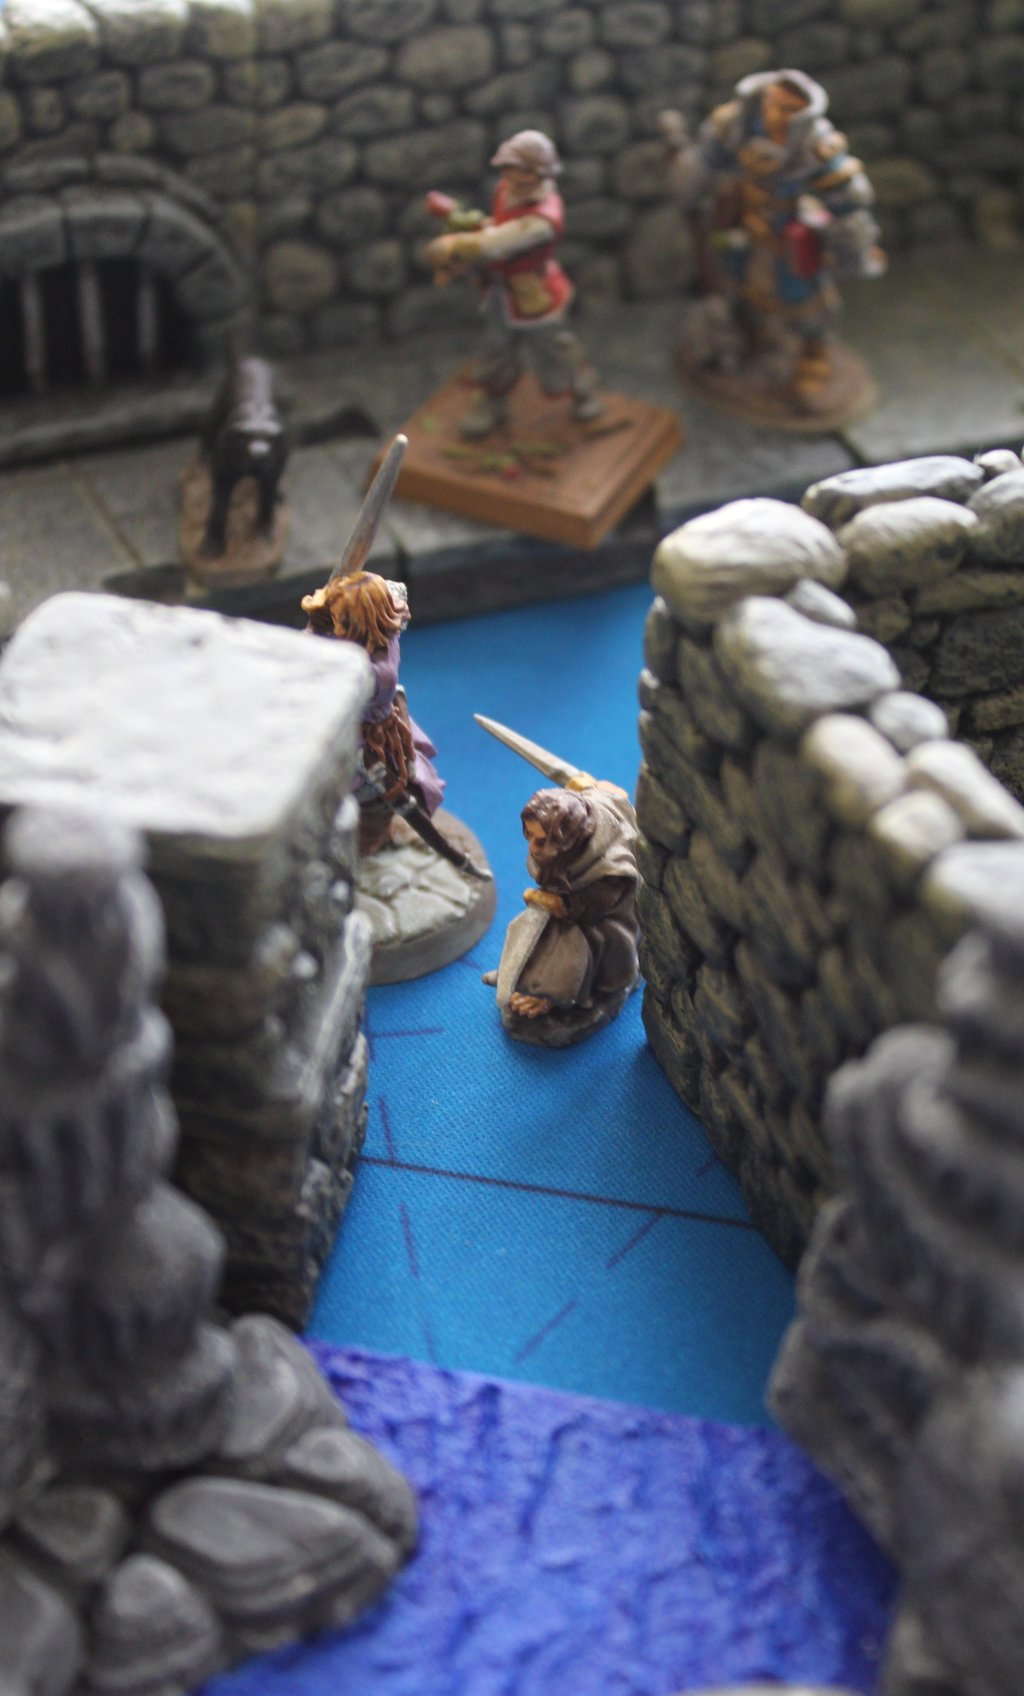
\includegraphics[width=0.39\textwidth]{images/Korvosa-entrance-to-wererat-den-503383346.jpg}
	\caption{Korvosa entrance to wererat den}
	\label{fig:Korvosa-entrance-to-wererat-den-503383346}
\end{figure}

"We are here to talk to Girrigz about the sick rats and people. A mutual friend asked us to check on you to make sure you are okay", Quint answers.\\

"What do you mean, sick people? My people, you mean? My people are sick, as are our rat brothers", the creature interjects.\\

"You don't know, then? The people in the city are sick as well, maybe one in four is infected by now, and many rats as well", Sjo replies. "Some citizens blame you and we just want ascertain ourselves of the fact that this hasn't gone down wrong with you?"\\

"Hmmrr, so the people blame us ... again, while they are the ones who are guilty! It's always the same with you people ...", a much lower-pitched voice grunts from an opening in the other end of the room.\\

"Are you Girrigz? Meep Gildenglare sent us", Quint inquires.\\

"Meep, har har, that old little turncoat human lover ... she has turned from her own, we have no interest in what she has to say",\hyperref[fig:Korvosa-wererat-den-Girrigz-503384054]{ Girrigz } groans back. "No, ignorant intruders, we are not responsible for this mess, on the contrary, it is all a vicious plan of your kind to decimate my folk. It is humans who set loose the diseased rats on the city, when they had that ship sink in the river bend." \\

\begin{figure}[h]
	\centering
	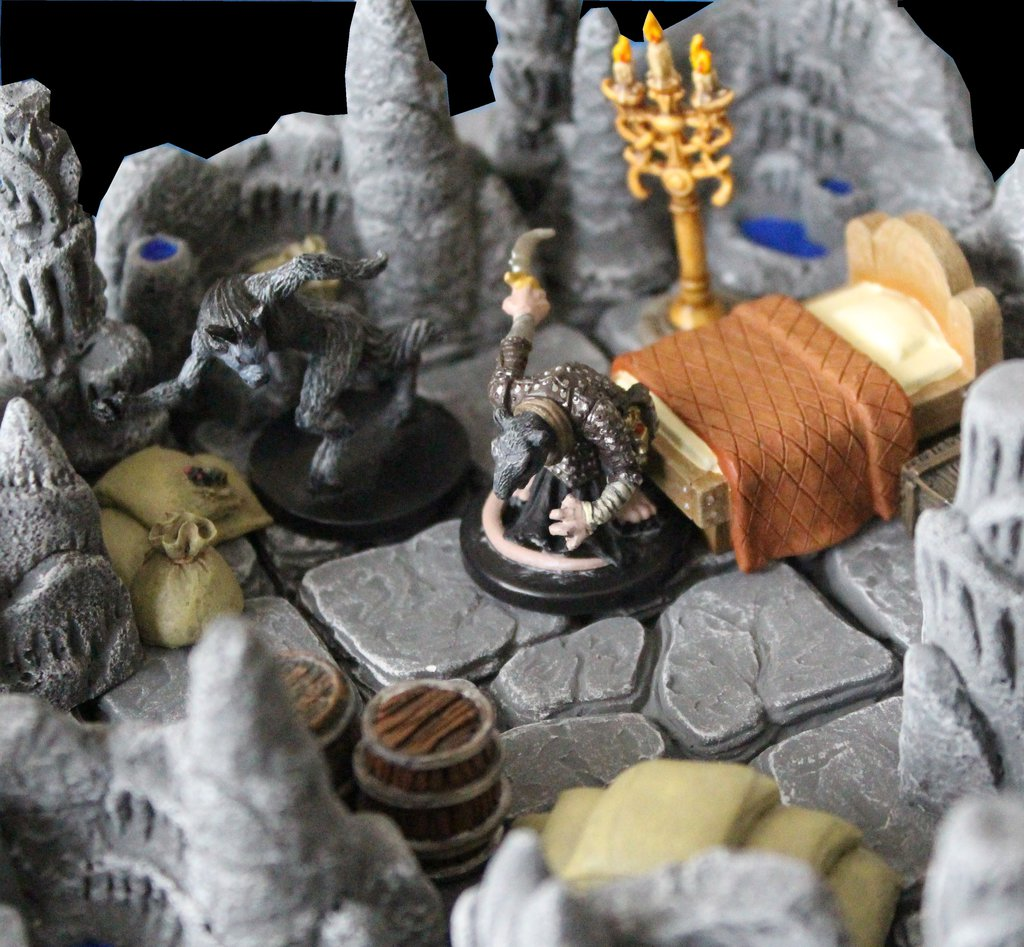
\includegraphics[width=0.39\textwidth]{images/Korvosa-wererat-den-Girrigz-503384054.jpg}
	\caption{Korvosa wererat den Girrigz}
	\label{fig:Korvosa-wererat-den-Girrigz-503384054}
\end{figure}

Quint realizes that the wererat does not have a correct picture of the situation above ground. "Well, first of all, it is definitely not 'all the humans' who are responsible. Thousands are sick as well and hundreds have already lost their lives. I'm even infected myself. So your analysis that the humans are responsible is not accurate. But I do believe you when you say that some humans might be responsible. Sometimes there are bad people and if you can offer any insight on what happened, we'd be happy to learn about it."\\

"So humans are sick as well ... the irony, struck down by your own kind! But don't you have healers up there who can make the sickness go away?"\\

"We do, I am somewhat of a healer myself", Sjo returns. "But the plague has taken on huge proportions, so we are struggling to save just a few. Still, you have sick here as well? I can have a look at them if you want me to, although I do not master the magic to heal them."\\

"Well, maybe I do ... that is to say, I am in possession of a magical wand that is supposed to heal the sick, but I lack the power to activate it. Maybe you are capable of doing so?" Girrigz inquires with a friendlier voice. "I'll send one of my brothers to fetch you, follow him, but only you, big man, the rest of you will remain where they are."\\

The shifty ratman that Balian noticed before reappears in the north exit and waves Sjo closer. He leads the Shoanti through a smaller cave that reeks of death and decay. Hundreds of dead rats and at least seven deceased humanoids have been piled to the wall. The next room in the\hyperref[fig:Korvosa-wererat-sewer-dens-503381693]{ complex } is bigger, a small fire burns in the center and lights up the features of a dangerous-looking wererat, obviously Girrigz. Four very sick wererats are lying on the floor and more lycanthropes and dire rats move in the background. Quint sees that some of them shows signs of the plague as well. \\

\begin{figure}[h]
	\centering
	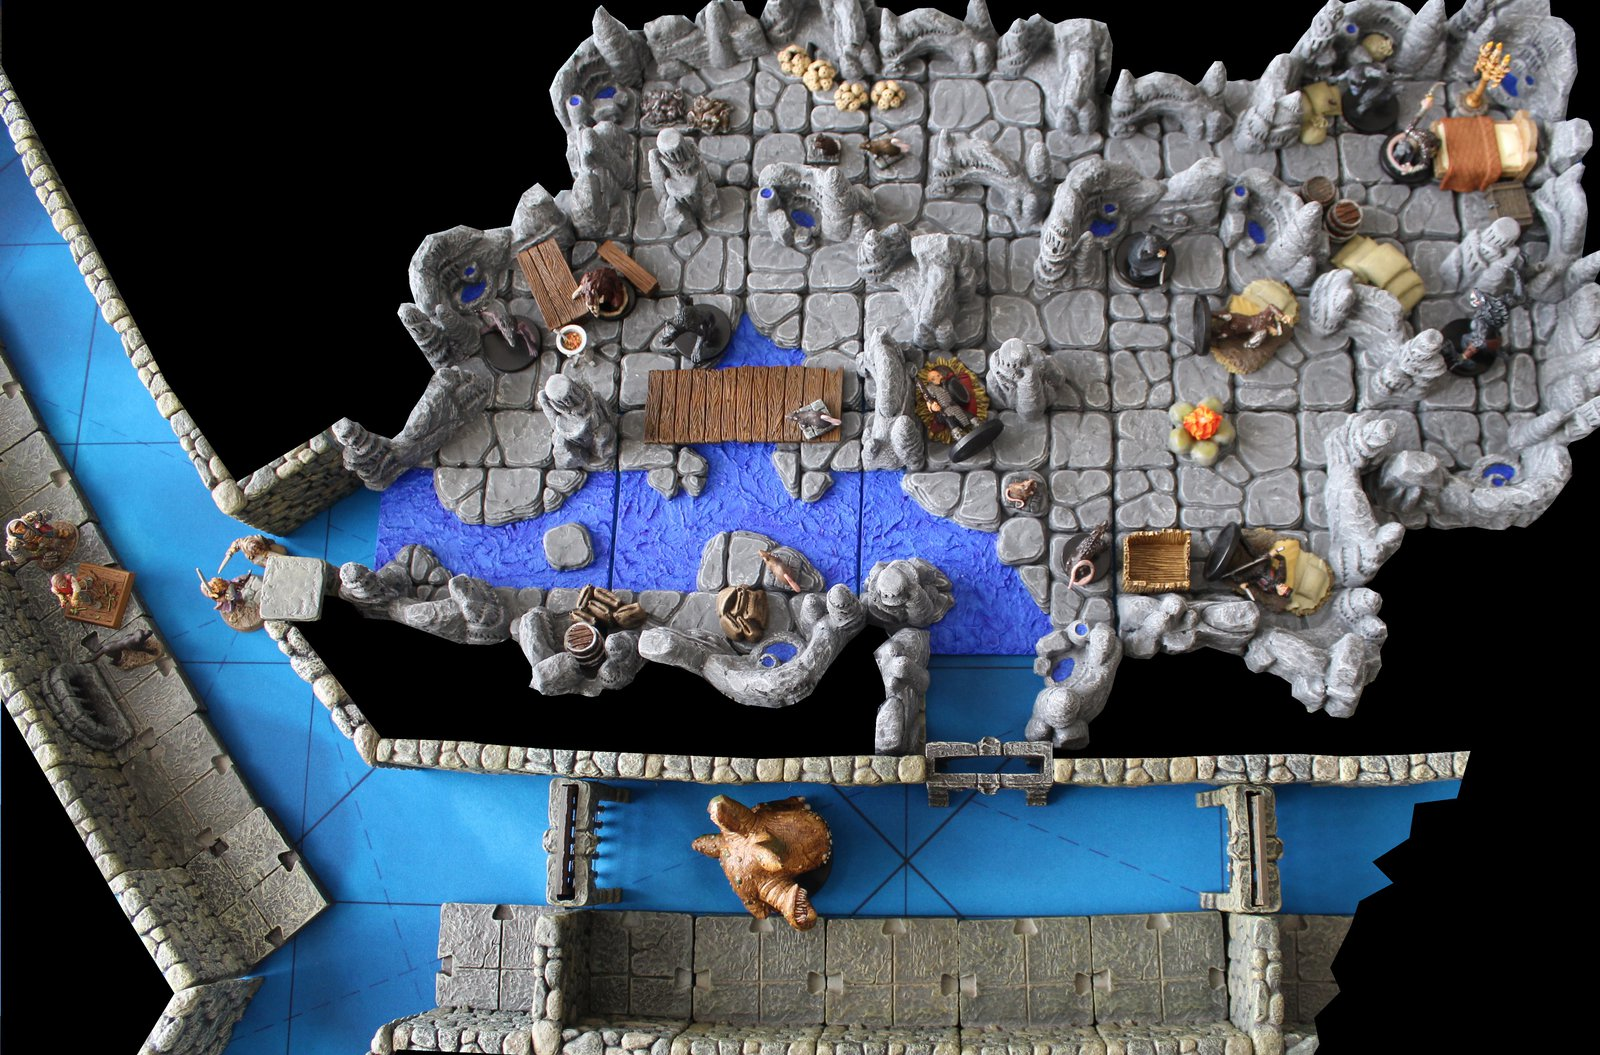
\includegraphics[width=0.39\textwidth]{images/Korvosa-wererat-sewer-dens-503381693.jpg}
	\caption{Korvosa wererat sewer dens}
	\label{fig:Korvosa-wererat-sewer-dens-503381693}
\end{figure}

The healer examines one of the diseased creatures, he won't last another day if he receives no care. Girrigz comes closer and hands Sjo a white wand. "It should contain the magic to cure diseases." Sjo accepts the item and moves his other hand inside his pocket to reach for Zellara's deck. The fortuneteller's cards confirm that the wand does what Girrigz says. Of course, Sjo realizes, there is only a limited chance that the magic will have the desired effect. By his calculations that shouldn't even be one in two since wands are usually made at minimal caster level. Furthermore he does not know if the wererat is aware of that; so he tries to formulate it in a simpler fashion: "Your men are in bad shape, I'm afraid. I hope they are not too far gone to be cured. There, let me try it on this poor man first." Sjo activates the magic and the wererat immediately lets out a sigh of relief as his sores disappear and a healthy blush returns to his cheeks. So fortune favored the Shoanti on this first patient, but there still are three more badly diseased lycanthropes in the room. Sjo's attempts to cure these creatures meet with less success, as only one of them gets better. Sjo even retries healing the last one with a second charge, but that fails as well. "I'm afraid your brothers are too far gone", he whispers, knowing all too well that failure has nothing to do with the patient's condition, but with the strength of the wand. When Girrigz seems to accept this fact, the Shoanti is relieved, but he quickly fears that his little bluff might be pierced when Girrigz asks him to cure three other less sick wererats. Still, fortune favors the Shoanti once again as all three attempts to cure these three succeed on the first try. So his story holds.\\

Girrigz is now fully convinced of the companions' good intentions and invites all of them into the room to negotiate. When Sjo tells him that the magically cured are not immune to the disease and might get infected again, the wererat leader nods and suggests that it might not be a bad idea to lead the sick rats out of the city. The fierce lycanthrope looks nothing like the pied piper from the fairy-tale, but he might have the same sway over rodents and taking the infected rats out of the city would be a giant leap in fighting the plague.\\

Girrigz also confirms what the companions suspected already. The mysterious plague is connected to the ship that sunk in the harbor over a week ago. The wererat was alerted to the burning vessel by one of his rat friends. He went to the exit of the east tunnel to witness the ship go down, as hundreds of rats fled from the wreck. "It is customary for a boat to hold a few dozen rats, but this ship had far too many of them, many hundreds, some of whom swam to my location. That was the first time I saw the festering sores that have since then taken out half my crew. Strangely enough, there were no human survivors trying to reach the shore."\\

The companions decide that the wreck deserves closer inspection. Still, they were sent here with a mission as well, making sure that Girrigz does not take out his ire on the humans above. Sjo steers the conversation in this direction again, but first he wants to improve his goodwill and digs out the {\itshape restorative ointment} from his pack, knowing that this salve has the same chance to cure the sick as the wand did. "I might have one more trick up my sleeve to help your sick friends", he says. He applies some of the ointment on the last two sick wererats and as if by a miracle, they both work! Girrigz is very interested in the unguent and proposes to trade it for the wand. Sjo immediately sees the gain in this deal and accepts: there are only two applications of ointment left, while the wand still holds twenty charges. On the other hand, the wererat leader has no use for a wand he cannot activate, so it is a win-win situation. When the companions ask Girrigz not to seek revenge on the humans, he quickly agrees. The thought had crossed his mind, but the information and the aid the party provided him and his people sufficed to sway him. The company parts in good spirits. That evening Sjo uses the wand to cure the children in the villa and little Brienna. He also secures a sloop for tomorrow and arranges with Larella that she will forego one {\itshape cure disease} spell in favor of some  {\itshape water breathing} magic. 

	%!TEX root = ../crimson_throne_book_main.tex
% 2014-12-31
\section{30 Sarenith 4708}

On the way to the harbor the companions pick up a copy of the {\itshape Korvosa Herald} . They are happy to see that their call to aid the city's medic force has made it to the front page. Larella casts {\itshape water breathing} on the party before fisherman Jarend takes them out to the river bend where the ship sank. Quint spots a shadow on the bottom of the stream that looks like the wreck. He pulls out his wand of  {\itshape mage armor} to enhance everyone's defenses, as swimming in armor is not a good idea, even with the ability to breath under water. Then the companions dive to the sunken ship, which rests some 70 feet below the water line on the bottom of the river. A moniker on the bowsprit identifies the vessel as the  {\itshape Delivery} , the same ship that bore off necromancer Rolth almost two months ago. The strangest feature of the wreck is a big hole in the hull with a massive ballista arrow sticking through it. This hole was obviously below the water line when the boat was still afloat, and must have been the main reason why the ship sank so quickly. What is weird about the arrow, is that it sticks out of the hull instead of into it. It was fired from within! The deck is blackened by the fire that raged there before the ship went down. Especially the aft deck was badly damaged. Balian swims for the foredeck first and kicks open a door that was swollen shut. Inside he finds a room that was converted to a shrine of Urgathoa. A crude wooden statue of an attractive, straight-haired woman with a lower body that has wasted away to bones leaves no mistake as to her identity. If this ship bore the disease that plagues Korvosa, the goddess of physical excess, disease and the undead would make for a fitting patron deity. Puk even notices Urgathoa's unholy bible, {\itshape In service of Your Hunger} , floating in the water. Fortunately the ink has mostly faded from the pages. The doors the cabins in the aft deck open more easily, as they are almost burned through. The right room is a small mess hall, while the left one used to house the captain. The contents of these rooms were mostly destroyed by the flames, but the captain's quarters still hold a valuable clue. Nailed to the wall are the burned remains of a\hyperref[fig:Burned-map-for-curse-of-the-Crimson-Throne-503803899]{ map } , showing the Bay of Korvosa. One location is marked in red: Lost End, a place on the desolate south coasts of the bay, where the dangerous cliffs normally don't allow ships to moor. Quint has heard of this place before: Lost End was once the country house of the Porphyria family, a noble house that was exiled from Korvosa by King Eodred's mother, Queen Domina, after they tried to steal the crown from the Arabasti dynasty. Fortunately Chadris Porphyria's short reign was such a disaster that it paved the way for Domina to seize power for her family again. The surviving Porphyria's returned to Cheliax, where their house still held a lot of power. Perhaps the plague is their revenge or a devious way for them to facilitate their return. \\

\begin{figure}[h]
	\centering
	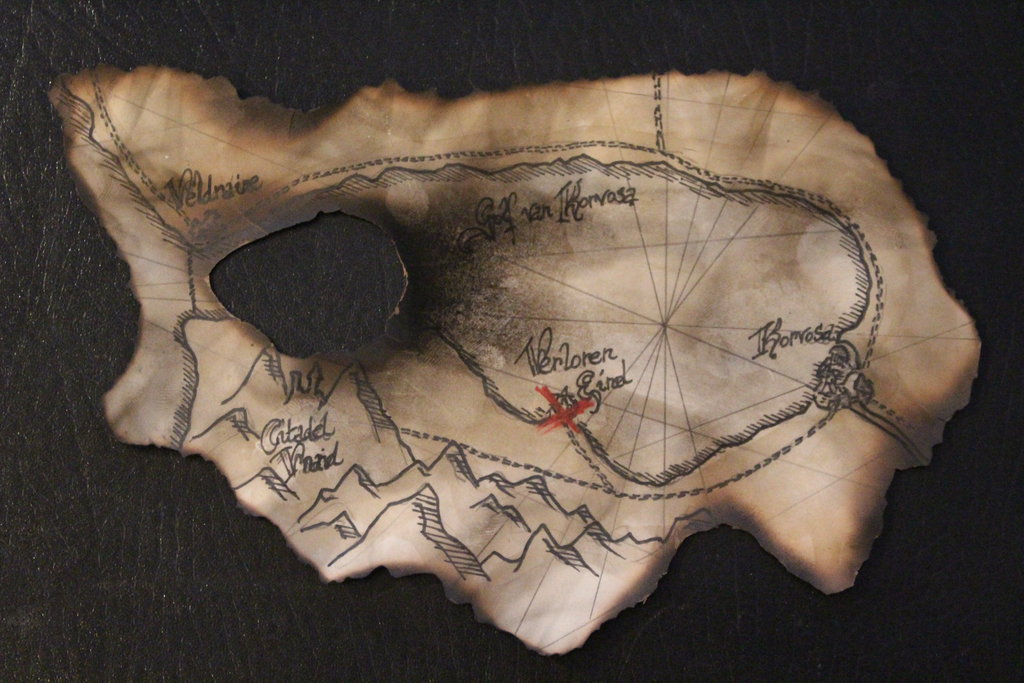
\includegraphics[width=0.39\textwidth]{images/Burned-map-for-curse-of-the-Crimson-Throne-503803899.jpg}
	\caption{Burned map for curse of the Crimson Throne}
	\label{fig:Burned-map-for-curse-of-the-Crimson-Throne-503803899}
\end{figure}



	%!TEX root = ../crimson_throne_book_main.tex
% 2014-12-31
That is a nice map, what did you use to make it?\\



	%!TEX root = ../crimson_throne_book_main.tex
% 2015-01-01
Just some paper that looks like parchment, which you can get in the store. I drew the map on it and burned it. I actually tried making a computer version first, but since I don't have any decent graphic software, it was easier to do it by hand and burn it for real (obviously a controlled fire, taking out or blackening the part I wanted to get this result). It makes for a nice prop, though.I sometimes use the same parchment paper for other hand-outs as well, e.g. I have a translated version of For my copies of the 

	%!TEX root = ../crimson_throne_book_main.tex
% 2015-01-03
The companions want to explore the sunken {\itshape Delivery} further and make their way through the hatch into its cargo hold. Swimming inside they see they are not alone: \hyperref[fig:Examining-the-wreck-in-Curse-of-the-Crimson-Throne-504554608]{ a giant octopus moves in to attack } . Quint throws a  {\itshape cacophonous call} on the bottom dweller, nauseating it and forcing it to retreat in the galley. Slowly the heroes swim towards the door, but before Sjo can close it, Balian sneaks through and swings his greatsword at the large creature. Hampered by the water, his hit loses much of its strength. Puk stabs at it as well, but as the octopus has taken up position in the corner, there is no way for him to hit its vulnerable spots, so his cuts are only minor nicks. It seems like both heavy hitters have lost their advantage in this underwater environment. When Quint's spell is about to end, the bard tries to renew it, but this time his magic is resisted and the sea creature regains control of its actions. Its tentacles lash out and all the companions suddenly find themselves in the awkward grasp of rubbery arms. Balian has to drop his blade and pulls out a simple dagger to cut at his opponent. Sjo does the same, but finds it hard to score a hit. Quint, who is usually the least effective melee fighter, is all of sudden the biggest threat as his  {\itshape short sword of frost} pierces one of the tentacles, rendering it useless. The iron embrace of the octopus's arms slowly squeezes the life out of the heroes as they try to fight themselves free. Although they manage to cut off more tentacles, the crushing arms take their toll and both Sjo and Balian lose consciousness. Puk and Quint are near to the end as well: the halfling lashes about furiously with his small swords, scoring some extra scratches, but Quint saves the day by striking the final blow. \\

\begin{figure}[h]
	\centering
	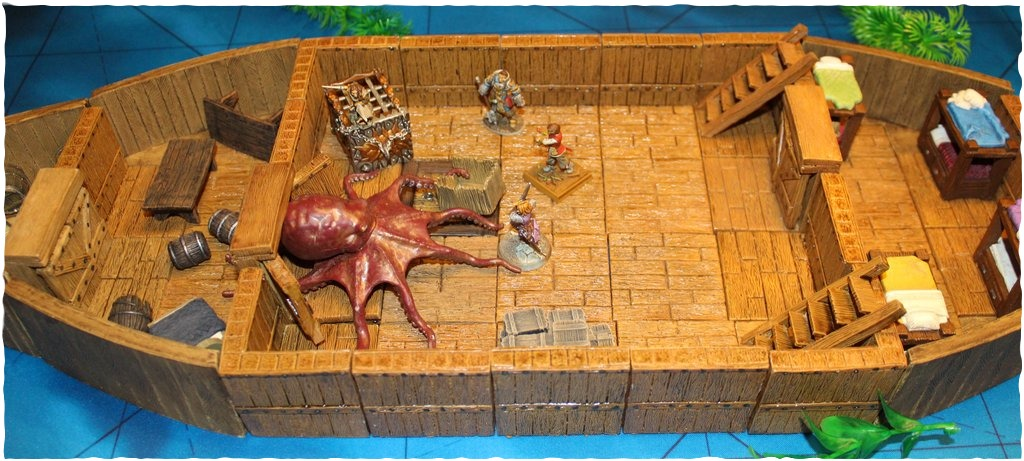
\includegraphics[width=0.4\textwidth]{images/Examining-the-wreck-in-Curse-of-the-Crimson-Throne-504554608_mod.jpg}
	\caption{Examining the wreck in Curse of the Crimson Throne}
	\label{fig:Examining-the-wreck-in-Curse-of-the-Crimson-Throne-504554608}
\end{figure}

The companions take a few moments to heal up, before searching the cargo. There are over half a dozen big cages, the doors of which have all been opened. Each of these holds a number of dead rats, who did not die from drowning, but rather from the plague. In the lower hold the companions discover more opened cages, as well as the drowned body of a man who has an amulet of Urgathoa around his neck. There is also a ballista in here, that was used to fire the heavy shaft through the hull which caused the vessel to take on water and sink.\\

The companions return to the harbor, dry up and head to the citadel to report to Field Marshal Cressida Kroft. She encourages the heroes to examine the location marked on the map: the abandoned Porphyria manor {\itshape Lost End} . She will make a document to authorize her special task force, so the companions do not run into trouble again because they cannot prove they are working for the city. She asks them to make preparations and return tomorrow to pick up the document. The companions spend the rest of the day getting ready for their trip. They also make sure that Tayce and Brienna have enough food to get through the next couple of days without having to leave their house and risk exposure to the plague. They do the same for Madam Nesia and the children in the villa.\\

Quint also dives into the villa's library and finds more information on {\itshape Lost End} . The country house was commissioned by Lord Chadris I of House Porphyria. This nobleman was one of the wealthiest and most prominent businessmen and aristocrats in the city in his day. He was also the direct competitor of Eodred I, who was crowned the first king of Korvosa, much to Porphyria's discontent. One of Chadris's wilder business ideas was to buy up the desolate lands on the south coast of the Bay of Korvosa and try to establish a harbor there. He never got past one small landing stage in a cave, somewhere in the fierce cliffs that line the south edge of the Bay and a large manor on top of the rocks. The waters proved too treacherous to allow for any decent harbor activity and the political struggle for power in Korvosa consumed too much of his attention, so Chadris abandoned his plans to develop the area further. The manor became the Porphyria holiday house, although it found a more permanent resident in Lady Ulrika, the wife of Chadris' son, Chadris II, and mother to Chadris III, who briefly made it to the throne of Korvosa, becoming its worst and most unpopular king to date. Lady Ulrika reportedly resided in the manor for health reasons, but the truth was that she was insane and her family locked her away in the country house to avoid embarrassment in the higher circles of the city. Since the fall of the Prophyria's, at the end of Chadris's mad reign, and their banishment to Cheliax in 4667, the manor has stood empty. Since it is the last day of the month, Sjo pays a visit to the tax office and declares what the party made in the last month. Taxes amount to 4,819 gold sails, due to be paid over the next month.\\

That night Balian and Quint are awakened from their sleep by cries from Nesia's room. The girl is having a bad dream. Balian carefully wakes her up and tries to calm her down. She says she had a nightmare in which she saw the shadow of a robust man standing in a doorway. He said something to her and then closed the door, after which blood started dripping from the ceiling, slowly filling the room. As Nesia is quite shaken, Balian offers to sleep in the extra bed to watch over her.\\



	%!TEX root = ../crimson_throne_book_main.tex
% 2015-01-03
\section{1 Erastus 4708}

The companions get their horses ready for the trip to {\itshape Lost End} and pick up their charter at Citadel Volshyenek. The Field Marshal also hands them a reward for closing Lavender's Luxury two days ago: a hefty pouch with 1,000 gold sails and some of the swindlers' equipment, a magical greatsword, mithral breastplate and cloak, which all go the Balian, and a  {\itshape ring of protection} for Quint. Then the heroes leave the city. The farmland makes way for a rougher terrain after a couple of hours as the road bends off to the west and crawls between the western stretches of the Mindspin Mountains that line the southern horizon and the cliffs alongside the Bay of Korvosa somewhere to the north. The sole pathway here sees infrequent passage, as only the Hellknights from Citadel Vraid travel it from time to time on their heavy warhorses, but the heroes do not encounter any of these blind enforcers of the law today. When darkness sets, they make camp and pass a restful night.\\

\section{2 Erastus 4708}

After a couple of hours Balian spots an overgrown path that veers off the main road to the northwest. Travel becomes slower now, as the horses have to walk through the high grass and weeds. It definitely looks as if no one has come this way for a long time.\\

It is almost noon when the companions pick up the muffled murmur of pain from behind the bushes. They dismount and check out the source of the noise, discovering a large wounded bear that has a bear trap around its paw. It has been pulling at the iron teeth to try and get free, but its efforts have only caused it further injury. The animal roars viciously when the adventurers approach, giving them pause. Suddenly the growls of the injured colossus are drowned by barking dogs, who are closing in fast. A few breaths later six hunting hounds burst out of the foliage and attack both the bear and the companions. Despite their fervor the dogs cannot penetrate the companions' defenses and soon start to fall prey to their weapons.\\

"You hurts my dogs! Rukus Graul kill you for that, he will!" The master of the hounds arrives in the wake of his pack. It is an\hyperref[fig:Rukus-Graul-504564975]{ ugly humanoid with a wide mouth and a huge misshapen finger which dangles like a hook from his right hand } . Quint recognizes the creature as ogrekin, like the grotesque cabbage-headed hulk the heroes encountered in the derro warrens, an unnatural mix of humans and ogres. The lumbering hunter wields a sharp spear, but fails to hit Balian. At the same time the hounds finish off the bear and now hurl themselves on the companions. The heroes pick off the mongrels one at a time without suffering a single bite. The unfortunate half-ogre is equally unsuccessful and never scores a hit with his spear. Sjo barks at him to surrender, but he refuses. "You kill my dogs, I kill yours!" he grunts as he plunges his pike in Spyder. "Rukus not surrender, ever!" he shouts as the companions bear down on him from all sides. The next moment his dead body drops to the ground. That is how the heroes of Korvosa deal with stupid, overconfident brutes. \\

\begin{figure}[h]
	\centering
	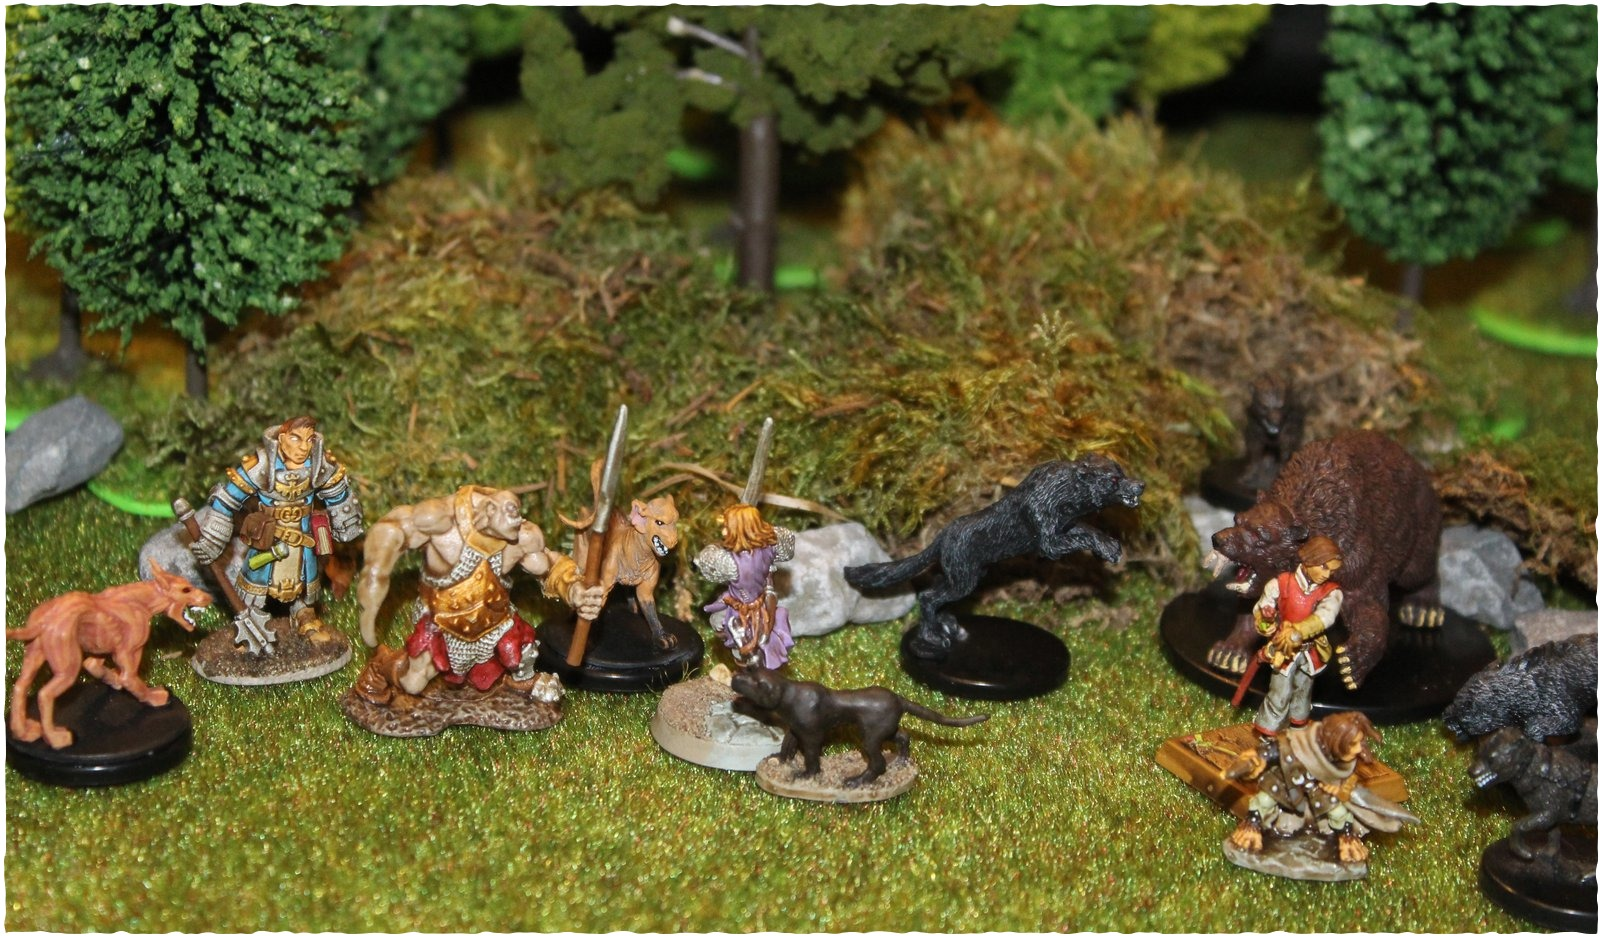
\includegraphics[width=0.4\textwidth]{images/Rukus-Graul-504564975_mod.jpg}
	\caption{Rukus Graul}
	\label{fig:Rukus-Graul-504564975}
\end{figure}

Using {\itshape detect magic} Sjo is pleasantly surprised to learn that this primitive creature was wearing a valuable girdle around his waist, a  {\itshape belt of giant strength} , which the Shoanti healer gladly straps around his own hips. 

	%!TEX root = ../crimson_throne_book_main.tex
% 2015-01-03
Unless you are not familiar with {\itshape Rise of the Runelords} you will surely have recognized Rukus Graul from  {\itshape The Hook Mountain Massacre} . Be sure to chime in for the next sessions if you want to see more from Nick Logue's wonderfully horrible module in this little sidetrek adventure. 

	%!TEX root = ../crimson_throne_book_main.tex
% 2015-01-17
Looking at the cadaver of the brown bear that the ogrekin's hunting dogs took down, Balian realizes it has a nice, thick pelt that would make an excellent rug for his bedroom. With Puk's aid he starts skinning the magnificent animal, while Sjo tries his hand at preparing a juicy bear steak. When the companions finally return to the road where they left their horses, they are surprised to find their mounts missing. Fortunately whoever took them did not bother about hiding his tracks, so Balian easily picks up a trail. About an hour down the road the heroes discover two wooden buildings off the road, next to a clearing in the wood.\\

Puk sneaks closer to scout ahead. The two sagging buildings look like a worn down hunting lodge and barn. Windows have been boarded over and moss and fungus grow on the shaded sides of the decrepit structures. The halfling also spots a tangled field of corn and other diseased plants growing in the clearing.\hyperref[fig:Crowfood-Graul-507695369]{ An eight-foot tall brute } is working the ground with a vicious iron hook. His grotesquely deformed head resembles a giant pumpkin: a huge mass of tumors and overgrown bone gives his head a lopsided look. Numerous crows fill the air above him. Puk circles the lodge, sticking to the trees, and makes his way around the building to the barn. Upon approaching that building he quickly makes out the frightened whinnying of horses, cruel chuckles of more brutes and savage snarls of dogs inside. \\

\begin{figure}[h]
	\centering
	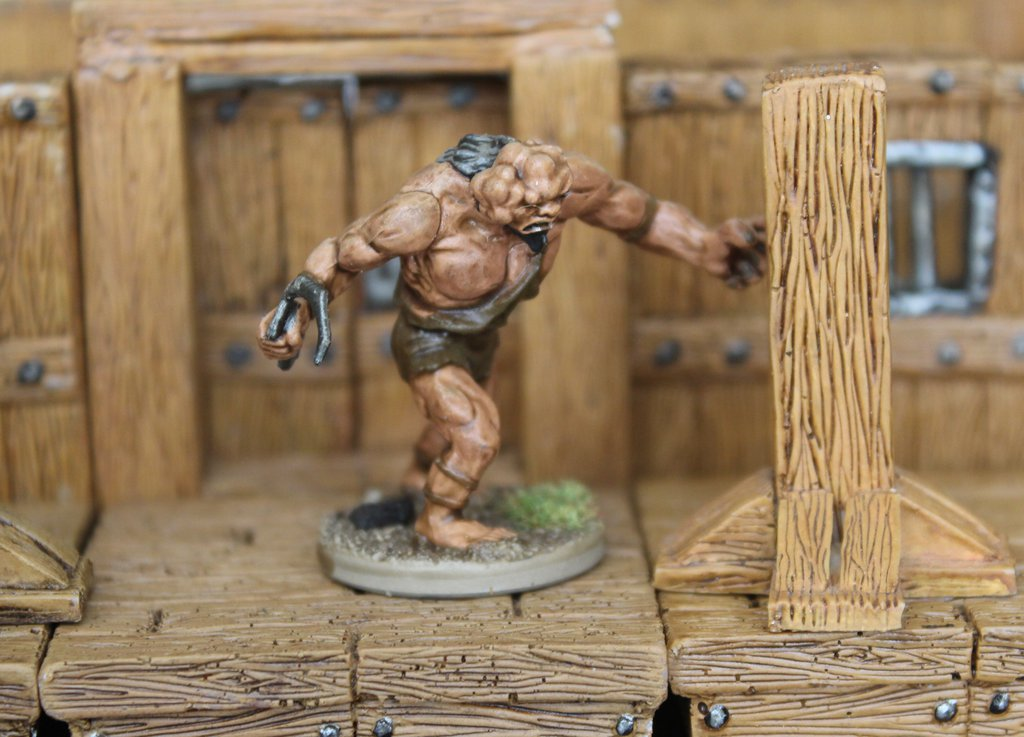
\includegraphics[width=0.39\textwidth]{images/Crowfood-Graul-507695369.jpg}
	\caption{Crowfood Graul}
	\label{fig:Crowfood-Graul-507695369}
\end{figure}

The halfling gathers his friends and together they stealthily crawl up to front of the barn. Puk throws open the doors and the companions look upon an unpleasant scene.\hyperref[fig:Graul-barn-507694269]{ Three ogrekin } and two skinny, naked dogs are torturing three awkwardly bound horses. Puk's riding animal seems to be taking the worst punishment and shows various cut and bite marks. Balian's and Sjo's mount are here as well, but there is no immediate sign of Quint's ride. Balian storms in, charging an ugly ogrekin who has two forearms growing from his right elbow. Quint swirls his whip around the crooked stumpy legs of an exceptionally short hillbilly and pulls him to the ground, so Puk can stab him in a weak spot while he's down. Meanwhile Sjo realizes that the third of the brothers in the barn is huge, even in his eyes, standing over eight and a half feet tall. This giant has a somewhat 'normal' face, although his eyes are very big and his skin is pale as the full moon. Balian wields his weapon to great efficiency, taking out one of the dogs and the short-legged brother in one mighty sweep. He next faces the wrath of the two remaining brothers, who hit him hard with their bare hands. Meanwhile the pumpkin-headed ogrekin who was working the field outside, has rushed to his brothers' aid. He throws himself on Sjo, dangerously whirling around his vicious iron hook. Balian and Puk take out another opponent: the tall hulk falls dead at their feet. The last of the three torturers smashes the ranger in return with his twin forearms, but Quint understand that fourth, pumpkin-headed brother is the biggest threat, as he is clearly more experienced in battles and packs a ferocious punch. The bard spellbinds the ugly brute with a successful  {\itshape cacophonous call} , causing a sickening head-ache to surge through his tumorous brain, taking away his ability to fight. The creature retreats to the door and flees the scene. In the meantime the companions finish off the last opposition in the barn, before chasing after the ogrekin who is fleeing around the barn. The heroes manage to corner him and - even though he regains control of his actions and dishes out some damage to Spyder - he succumbs quickly to superior numbers. \\

\begin{figure}[h]
	\centering
	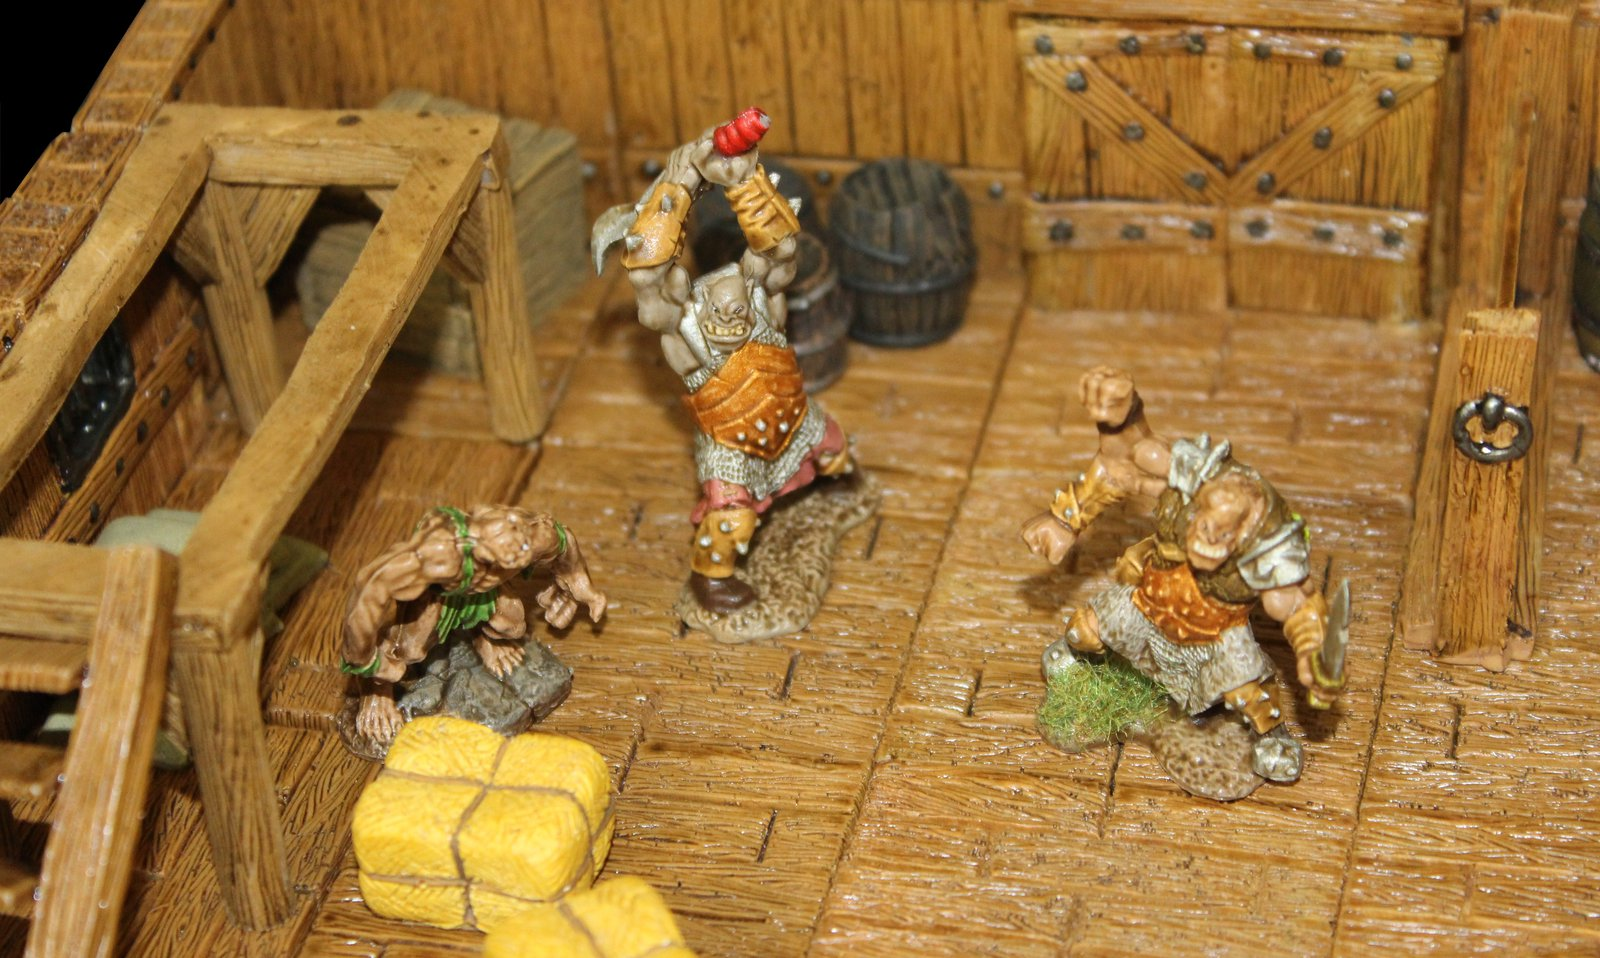
\includegraphics[width=0.39\textwidth]{images/Graul-barn-507694269.jpg}
	\caption{Graul barn}
	\label{fig:Graul-barn-507694269}
\end{figure}

With Quint's horse still missing, the companions decide to tackle the main house next. This decaying hunting lodge slumps drunkenly at the edge of the clearing. Rickety stairs crawl up to a porch covered by a huge eave which is supported by heavy pillars of pine. These timbers have crude carvings of manticores impaling children and wolves ripping apart women. The simple decorations look like a child's work, but the depictions grow more gruesome from one picture to the next. A large rocking chair of lashed wood and bone sways erratically in the breeze at the far end of the porch under a vast menagerie of wind chimes, all composed of humanoid and animal bones. The windows have been boarded up with thick timbers, although it is unclear whether this is to keep intruders out or to keep unspeakable horrors in. A host of ants marches happily away, many the size of a grown man's thumbnail. A moth as big as a shovel-head clings to the porch ceiling, watching the party with alienating eyes. The scent of bad meat, urine, sweat and decay wafts from between the cracks.\\

Sjo's warning that there might be traps is merrily laughed away, but when Puk walks up to the front door, a rack mounted with a series of sharpened bones suddenly swings down from between the many hanging bones. At the same time rusty saw blades spring from the cracks in the floorboards. The terrible double trap fails to hurt the lucky halfling, though, as the spikes only pierce the air above Puk's head, while the blades slides just left and right from where he's standing, cutting off no more than a few hairs from the tufts covering his ever-bare feet. The halfling chuckles at his own good fortune and slowly pushes open the door. The reception room holds a tremendous hearth in the right wall, but there is no fire burning in it, while the small rogue remembers that smoke arose from the chimney on the roof. A mangy dire bearskin rug lies before the fireplace. The animal's pained visage still snarls at whatever hunter that took its life. To the left is a huge couch, haphazardly upholstered in animal hide and humanoid flesh. Sjo recognizes a fox's head and a human-looking hand and foot in the putrid leather collection. The door on the other side of the room has a big hole in the bottom, big enough for Puk to see that the hallway behind it is clear. After having crawled through the hole, the rogue's keen ears pick up the exhausted cracking of wood. It comes from the door to his left, causing his curiosity to rear its head.\\

The halfling leads his friends down the hall and quietly opens the door. Next Balian storms in and faces an incredibly corpulent woman with stringy, black hair, greasily sticking to her humongous head. She wears an old stained curtain as a robe.\hyperref[fig:Mammy-Graul-and-ogre-Daddy-507696824]{ The room } reeks of sweat, but also of decay, which originates from the chamber's second occupant, a hulking ogre who did not come into view until Balian charged inside. The ranger realizes that this giant is no longer alive, although he still moves to attack the intruders. Could this be the deformed ogrekin's mother in the company of their late father, returned from the dead? It certainly seems so. Disgusted by the foul woman the ranger chokes and fails to hit her. "I don't know who you are, strangers, but you are fools for coming in here! I'll have your heads on a pike to decorate my porch! Daddy, tear them apart!" she shrieks. Balian turns to the ogre zombie and decides to attack him first. His greatsword tears through the rotting meat while Puk tumbles through the room to find an advantageous flanking position behind the undead hulk. The zombie moans and swings his heavy greatclub at Balian, but the ranger can block his strike. The fat lady rolls around in her bed - obviously the source of the creaking Puk heard earlier - and throws a heinous spell at the halfling which  {\itshape blinds} him. With one simple incantation she has stolen the rogue most powerful weapon, his eye for weak spots. Quint recognizes the woman's threat and tries to take her out of the fight with a  {\itshape cacophonous call} , but she resists his magic through sheer power of will. Sjo bludgeons her with his heavy mace, but cannot prevent her from draining Balian's strength with a  {\itshape ray of enfeeblement} . The sly mage has now crippled the second damage dealer with her magic. Balian gets no time to recover, for the ogre crushes half his ribs with a devastating blow. Quint attempts another  {\itshape cacophonous call} on the fat lady, but her will proves too powerful again. Sjo rushes to Balian's aid with a healing spell so the ranger can continue the fight, but the undead ogre hits about wildly, wounding all the companions. With Puk's and Balian's efficiency greatly reduced, it is hard for our friends to bring the giant to his knees. Both Spyder and his master go down first, before Puk can finally deliver the finishing cut. Meanwhile Sjo has resorted to firing wave upon wave of  {\itshape burning hands} at the corpulent monster, who finds no protection from this magic among her five  {\itshape mirror images} . When her zombie bodyguard is beaten, she decides to play it safe and whispers the words of a powerful spell that  {\itshape dimension doors} her out of the room with a simple "poof". \\

\begin{figure}[h]
	\centering
	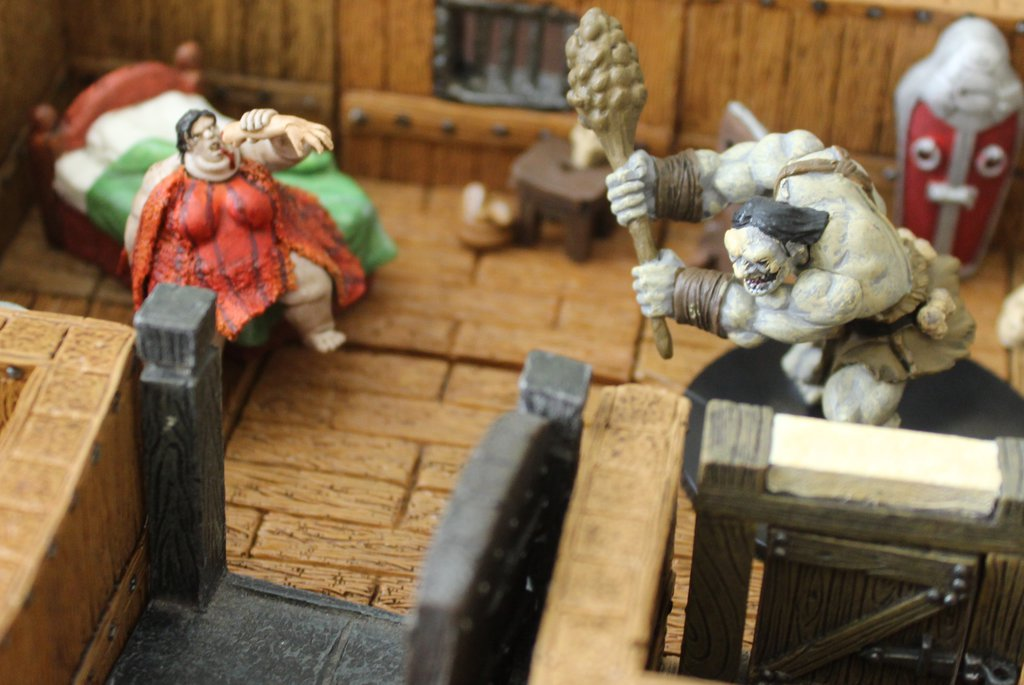
\includegraphics[width=0.39\textwidth]{images/Mammy-Graul-and-ogre-Daddy-507696824.jpg}
	\caption{Mammy Graul and ogre Daddy}
	\label{fig:Mammy-Graul-and-ogre-Daddy-507696824}
\end{figure}



	%!TEX root = ../crimson_throne_book_main.tex
% 2015-02-07
After they have recovered from the fierce battle with Mammy Graul and her undead ogre spouse, the companions search the rest of the homestead. With Puk still blinded and Balian still weakened by Mammy's necromantic magic, they proceed cautiously. The horrifying experience continues as they discover a dining room where the chairs are crowned with skulls and stretches with humanoid leather and a kitchen that has eyes and animal heads boiling in a stew. The stench of decaying flesh and excrement hangs thick throughout the building, accompanied by buzzing hosts of bloated flies. The young heroes confront one more hillbilly in the backroom. Although his frame clearly suggests that he is full-grown, the childish look in his eyes betrays his simple mindset. The hairless, malformed ogrekin smiles naively through his wide mouth of ragged teeth before he realizes that the men entering are intruders. He drops the humanoid baby skulls he was playing with and roars aggressively, flailing about wildly with his arms. Still, four adversaries and a dog prove too much of a challenge and he goes down easily. Quint draws back in horror as he examines the crude paintings in blood of grinning devils and dismembered animals on the walls, thinking of his horse that is still missing. Sjo ponders over the baby skulls: their grotesque shape makes him wonder whether these were ogrekin babies. Since all of Mammy Graul's children they have encountered so far were male, these small crania might be all that remains of her female offspring, toys for her sons. The upper floor proves less of a horror, housing one filthy bedroom and a junk-littered attic.\\

That leaves one more area to explore: the basement. The stairs lead down to a small hallway with three doors. The door on the right draws Balian's attention, as he hears the scraping sound of someone sharpening a weapon and the frightened whinnying of a horse. Puk attempts to push the door open, but finds it bolted from the other side, alarming the creatures in the room of the heroes' arrival. Quint quickly pulls the key-lock killer's magic bell from his pack and rings it, making the bolt pop free. The room reeks of rot and old blood. Piles of gore-spattered skin lie heaped on the floor. Quint's horse has been tied down to a large table, its legs are broken and it looks in bad shape, but still alive. A fierce-looking ogrekin towers over the table; hair grows lopsided from the right side of his head rather than atop his brow, but his left side reveals a more gruesome abomination: a second half-formed head grows from the back of his neck. It lacks the intelligent glare of the main head, though, and limits itself to grunting and drooling. The ogrekin orders two ratlike dogs to attack and roars out a threat in a language none of the heroes understand, although Quint recognizes it as {\itshape Giant} , the tongue used by ogres. In the other corner of the room, behind a second table, is Mammy Graul, who's shrieking encouragements at her son in Giant as well. Whatever she is yelling, it does not sound cordial, although Quint can make out that she calls the two-headed savage 'Hucker'. The\hyperref[fig:Grand-finale-in-the-Graul-homestead-basement-512310881]{ heroes rush across the room and engage the creatures } . Sjo focuses on the corpulent necromancer, noticing that most of the burns he inflicted earlier have been healed. His mace skitters off her layers of fat, but at least his presence menaces her enough to make her fizzle the spell she tries to cast. Puk stumbles forward blindly until he faces Hucker and one of the dogs. The luck of halflings protects him once more from the brute's deadly swing: the large metal hook tears into the ground instead of the unsighted rogue. At Quint's urging the halfling takes on a more defensive stance, since his puny attacks will not give the enemies more than a few scratches anyway. Meanwhile Balian and Spyder take out the second dog, but the ranger's decreased strength proves to be quite a handicap. Quint tries to support his friends by snapping around his whip and tripping Mammy and her son. The obese necromancer finds herself cornered by Sjo and resorts to her  {\itshape wand of magic missiles} , fearing to lose more spells in melee. Even though she can fire only two  {\itshape force} bolts at the Shoanti at a time, her continued efforts wear him down and finally force him to step back to heal himself. \\

\begin{figure}[h]
	\centering
	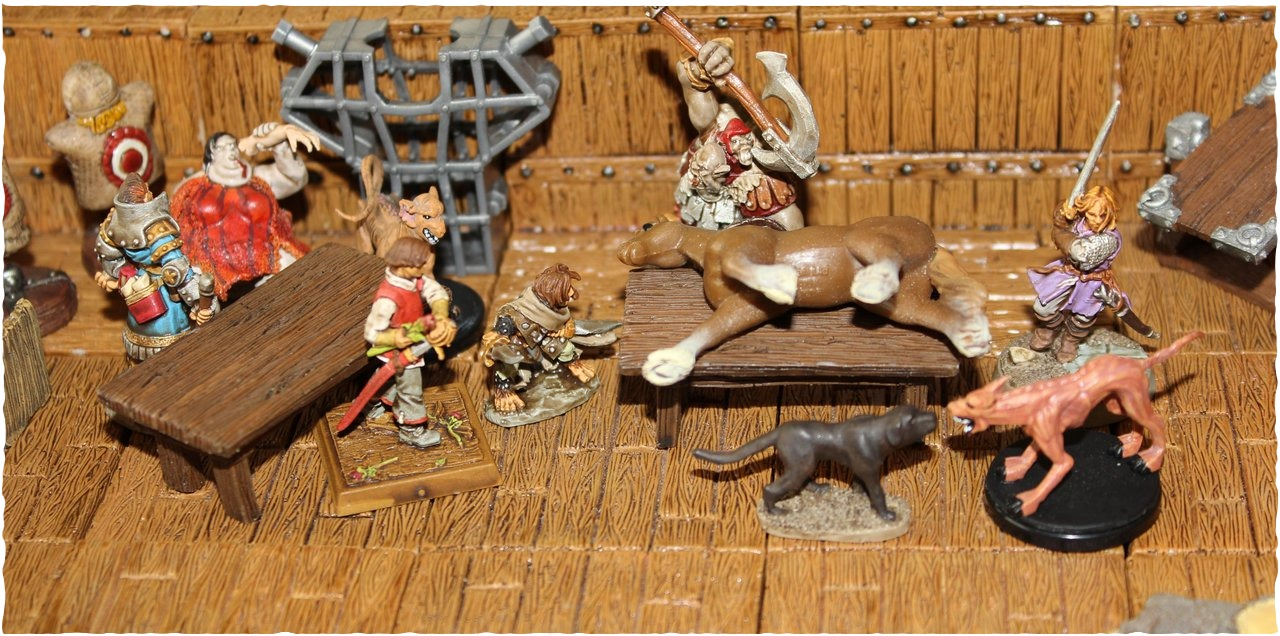
\includegraphics[width=0.4\textwidth]{images/Grand-finale-in-the-Graul-homestead-basement-512310881_mod.jpg}
	\caption{Grand finale in the Graul homestead basement}
	\label{fig:Grand-finale-in-the-Graul-homestead-basement-512310881}
\end{figure}

In the meantime the other heroes focus their attacks on the big ogrekin. Quint and Balian inflict several deep cuts, but the brute retaliates, dealing a mighty blow to Quint and hitting down Spyder. Balian presses the attack and finally finishes off Hucker with a critical strike. Sjo no longer has the magic to {\itshape outheal} Mammy and hits the floor as well. Once he ratdog has been taken care of, Mammy is the only adversary left. Hatred burns in her eyes as she keeps on firing  {\itshape magic missiles} at Puk now, who is next to lose consciousness. Balian now hits his greatsword into the fat monster's flesh, but it's Quint  {\itshape frosty} shortsword that delivers the final blow and ends this horrific conflict. The bard has just enough magic left to get Sjo and Puk back to their feet. Every potion, wand or spell that can provide healing has been depleted. Apart from Balian, who sustained no wounds in this last fight, all other heroes are barely alive. Getting some rest is a necessity, but first the companions make sure there are no more enemies about. Fortunately there aren't. As they search the rest of the basement, they find two more junk rooms and one large filthy prison that also serves as the building's cesspit. Manacled to the far wall is a strange man with goat-like legs and horns, a satyr. He is not conscious, although he is still breathing. His right arm has been chopped off, leaving only a bloody stump. This must have been the 'treat' Mammy Graul was chewing on when the heroes first surprised her. The companions free the faun and take him outside, where Sjo and Balian bind his wounds. The exhausted young adventurers spend the night in the barn at the side of their horses.\\

\section{3 Erastus 4708}

The companions take the rest of the day to recuperate and heal their wounds. Fortunately, Mammy Graul was smart enough to keep around at least one bottled cure to her own blinding magic in the form of a {\itshape potion of remove blindness} , which repairs Puk's sight, while Sjo's magic gives Balian his strength back. Quint's horse is healed of its broken legs and the heroes carefully bring back the satyr to consciousness. He is traumatized by this horrid experience, but Quint's kind words and music restore enough sanity so he can communicate. His name is Dernal, a satyr who lives here in the wilds. When he realizes that the threat has ended, he asks his rescuers if they have found his emerald necklace. This prompts a closer search of the lodge which reveals a secret cache in Hucker's basement room. A treasure chest holds some money and jewelry, as well as a pair of magical  {\itshape bracers of lesser archery} . 

	%!TEX root = ../crimson_throne_book_main.tex
% 2015-02-15
The companions take the rest of the day to recover from their ordeal at the hands of the Graul family. They consider burning down the hunting lodge, but despite the horror that the ogrekin brought to the place, it is a decent and sturdily built edifice. In the end the heroes decide to spare the building and burn the corpses outside on a large funeral pyre instead. Dernal, the satyr they saved, and Quint's horse seem to have withstood the worse of the trauma. The goat-legged man leaves for the forest to rejoin his kin, nodding his head in gratitude one last time and Quint's riding animal seeks comfort among his three brothers.\\

\section{4 Erastus 4708}

You might recognize Lost End, the abandoned Porphyria manor, as my version of Foxglove Manor, a.k.a. Misgivings, from The journey to Lost End takes just under three hours. The smell of the sea air and the cry of seagulls are the first signs that the companions are nearing their destination. Perched high above the ocean, on the edge of the cliffs, rests a stately manor house. Strong winds tear at the structure that looks poised for a suicide leap. That the manor clings to the top of the rocks is remarkable, as its far side hangs over a sheer drop down to the ocean below, a fall of over three hundred feet. The roof sags in several places and mold and mildew cake the walls. The house is crooked, its chimneys rise from various points among the rooftops, leaning like old men against the storm.\\

Four grinning gargoyles guard the front door and come to life when the companions approach. The demonic statues spread their stony wings and swoop down on the visitors. The heroes organize their defenses well and focus their attacks on one creature at a time, making short work of their enemies and minimizing the damage they take themselves. Since they have burned through every potion and wand that provides healing, they have to be careful with their resources, as only Sjo's and Quint's spells can cure wounds now.\\

The front door is barred from the inside, but the {\itshape Key-Lock Killer's bell} easily takes care of that obstacle. The entrance hall is \hyperref[fig:Pathfinder-Foxglove-manor-to-Lost-End-ground-floor-513919727]{ large and runs through to another room at the end of the house } , from where colored light streams in through beautiful stained-glass windows. A twelve-foot long monster towers over the visitors as they enter: its leathery wings spread out menacingly. The creature has the body of a giant lion, though its feline head is flanked by two more heads - a dragon's and a horned goat's - marking it as a chimera. The heroes draw their weapons before realizing that this fabled beast is not moving. It is a stuffed animal, a \hyperref[fig:Pathfinder-Foxglove-manor-to-Lost-End-chimera-513923128]{ magnificent trophy } from a long forgotten battle. The entrance hall sports other trophies along its walls, the heads of bears, boars and giant deer mounted on wooden display plaques. A lion's pelt covers the floor leading to the dining room in the back. A curving flight of stairs to the right winds up to the upper floor, and several doors provide entry to other rooms, their frames carved with scenes from the forest, the animals that inhabit the wilds and the hunters that chase them down. The house is definitely dirty, but the mold staining the floor, walls and ceiling does not carry the damp smell of decay that fifty years of degeneration should, suggesting that the place was aired not too long ago. Still, there are no signs of life anywhere now. The dining room in the back holds a large mahogany table. The cups and plates on it also show signs of recent use, no more than a couple of weeks ago. The stained glass in the windows is still intact and looks like excellent craftsmanship, but the colored glass blocks most of what would have been a breathtaking view of the Bay of Korvosa. \\

\begin{figure}[h]
	\centering
	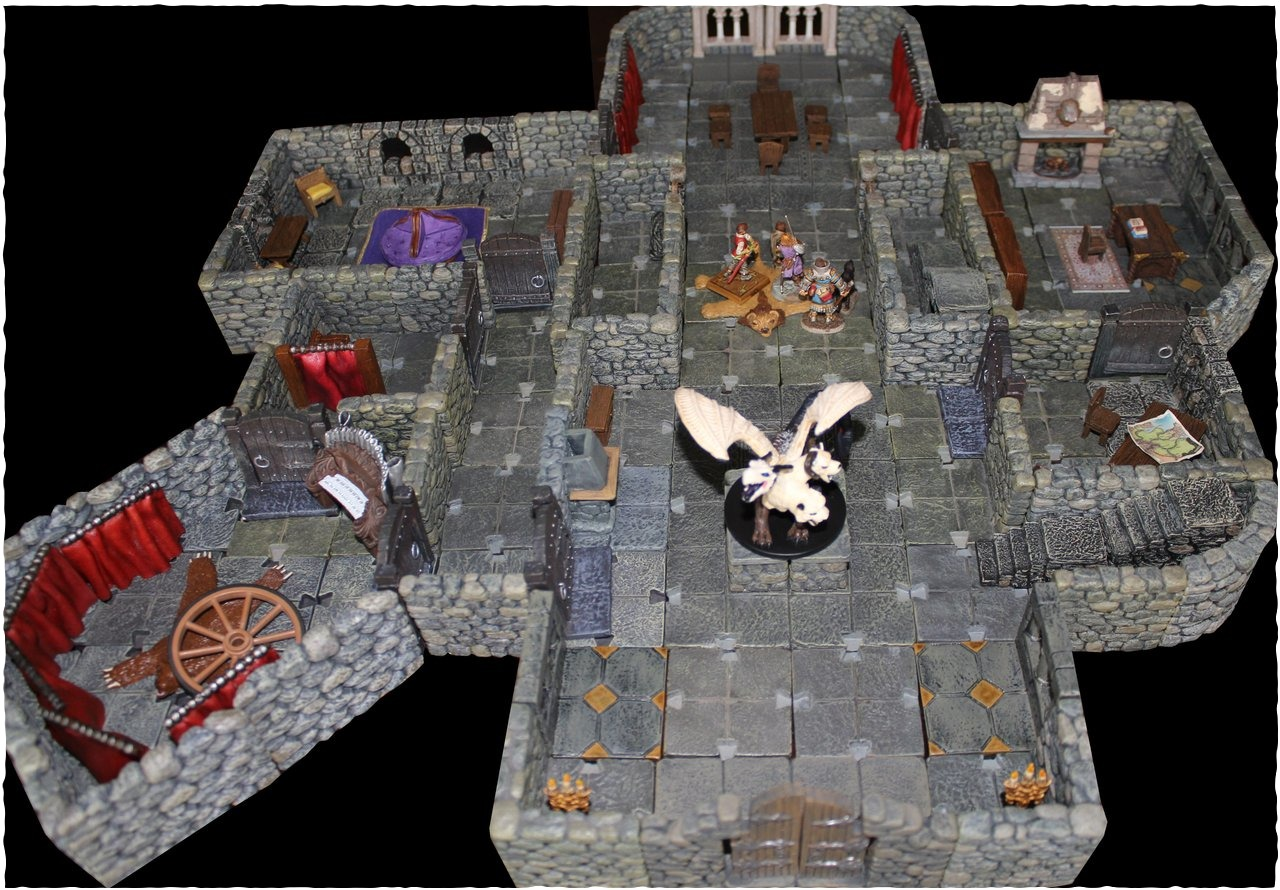
\includegraphics[width=0.4\textwidth]{images/Pathfinder-Foxglove-manor-to-Lost-End-ground-floor-513919727_mod.jpg}
	\caption{Pathfinder Foxglove manor to Lost End ground floor}
	\label{fig:Pathfinder-Foxglove-manor-to-Lost-End-ground-floor-513919727}
\end{figure}

\begin{figure}[h]
	\centering
	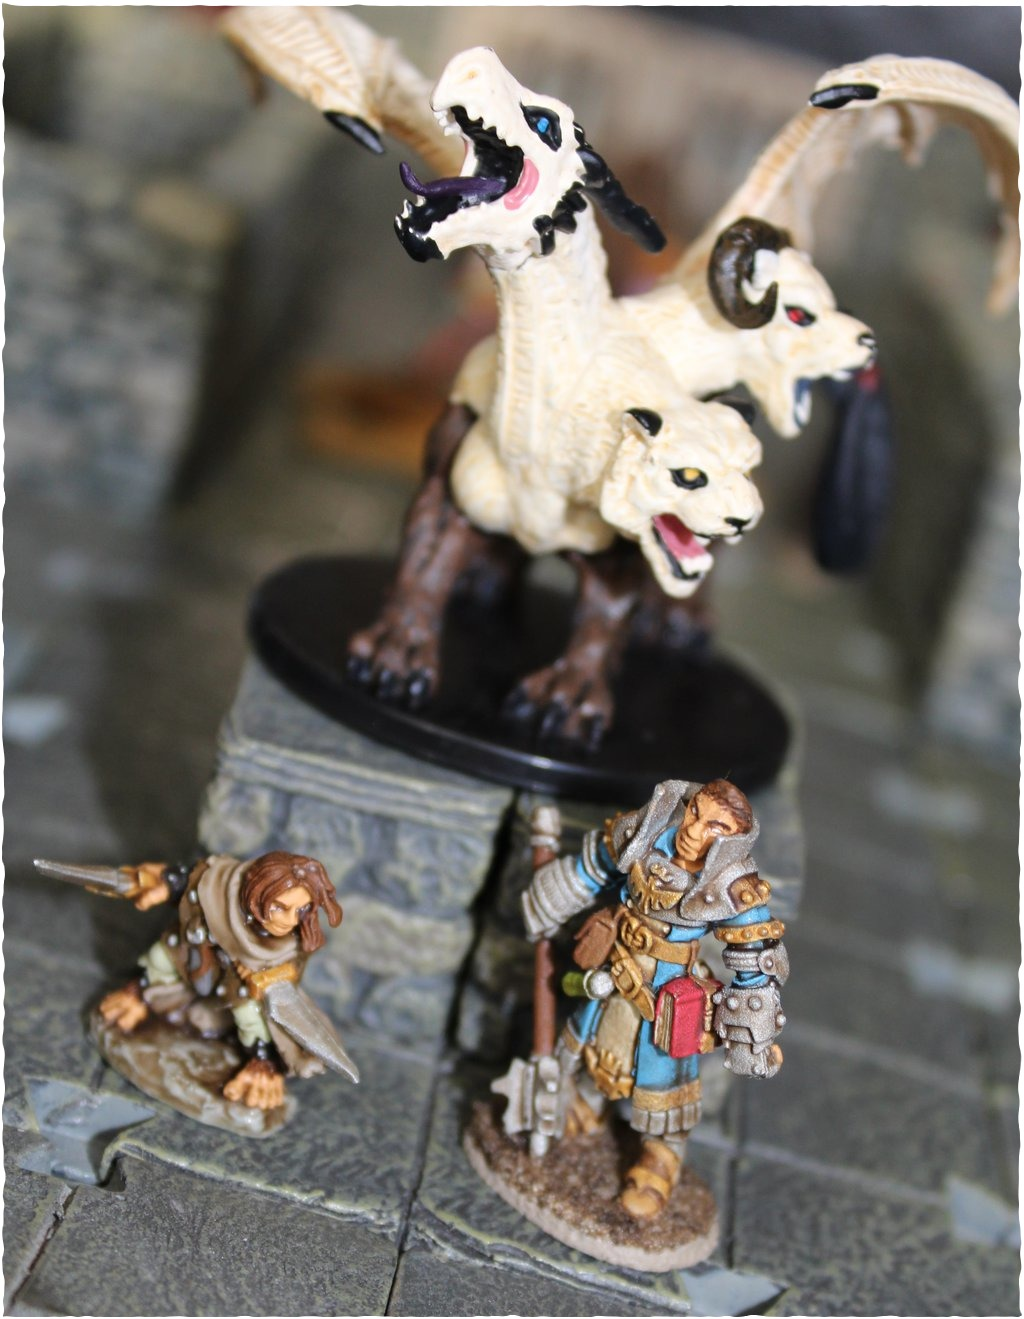
\includegraphics[width=0.4\textwidth]{images/Pathfinder-Foxglove-manor-to-Lost-End-chimera-513923128_mod.jpg}
	\caption{Pathfinder Foxglove manor to Lost End chimera}
	\label{fig:Pathfinder-Foxglove-manor-to-Lost-End-chimera-513923128}
\end{figure}

The companions make their way through the rest of the ground floor, including a dusty lounge and a\hyperref[fig:Pathfinder-Foxglove-manor-to-Lost-End-music-room-513922417]{ ruined music room } . The once-magnificent chandelier lies smashed on the floor, although the organ in the corner survived the crash. Still, half a century of disuse has not been kind on the instrument, which only produces false notes. The drawing room and library are cleaner and have obviously seen more use recently. The heroes discover notes on how to construct a flesh golem, including the creature's strengths and 'weaknesses'. The instructions also list the magic required to bring such a golem to life, with hard to find spells like  {\itshape geas} and  {\itshape limited wish} . The first would apparently be provided by someone called Andaisin, while the latter would come from a scroll. Quint suspects that these scribblings belonged to Rolth, the necromancer who took Balian's sister five years ago. \\

\begin{figure}[h]
	\centering
	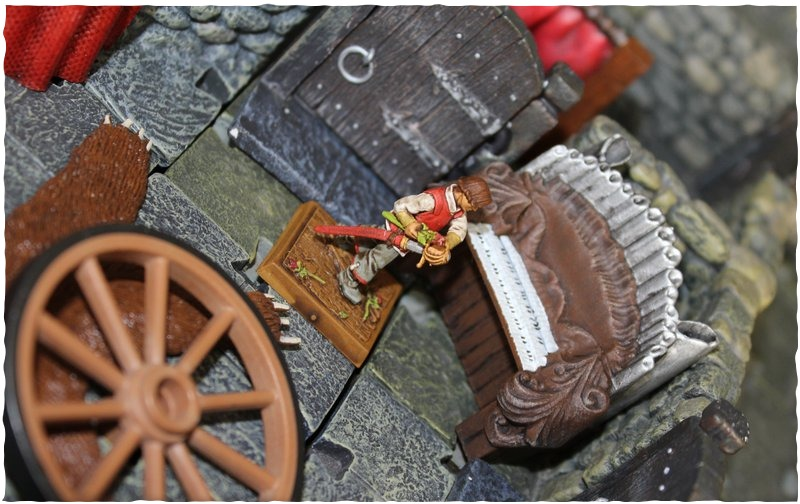
\includegraphics[width=0.4\textwidth]{images/Pathfinder-Foxglove-manor-to-Lost-End-music-room-513922417_mod.jpg}
	\caption{Pathfinder Foxglove manor to Lost End music room}
	\label{fig:Pathfinder-Foxglove-manor-to-Lost-End-music-room-513922417}
\end{figure}

Sjo rummages through more molded novels that are left on the bookshelves and some papers on the desk. He finds a document entitled the {\itshape plague plan} , that details the procedure on how to approach the Korvosa with  {\itshape the Delivery} . All passengers would leave the ship aboard rowing boats and make for the south of the city, while one person, named 'Rois', would stay on board and navigate the vessel into the mouth of the Jeggare River, where he would release the diseased rats, sink the boat and burn the evidence. The author of the note clearly had little respect for the suicide navigator, as he mocks the man for a fool. On\hyperref[fig:Pathfinder-Foxglove-manor-to-Lost-End-upper-floor-513924264]{ the upper floor of Lost End } the heroes discover a shrine to Urgathoa in the room above the dining room. \hyperref[fig:Pathfinder-Foxglove-manor-to-Lost-End-undead-513925444]{ Four skeletal warriors guard the unholy altar. } They throw themselves at the intruders, but like the gargoyles at the front door, they go down relatively easily, though not without delivering some vicious cuts with their rusted blades. Sjo heals his friends after the fight, but decides against patching up Spyder. The labrador sustained some gaping wounds and curing him would drain too many resources, so the companions leave the dog to guard the front door instead. The focal point in the improvised shrine is a statue of Urgathoa in front of the stained glass windows. Closer inspection reveals that this idol is actually a stone bust of a woman, named 'Lady Ulrika Porphyria', to which a skeletal lower body and arms were added. \\

\begin{figure}[h]
	\centering
	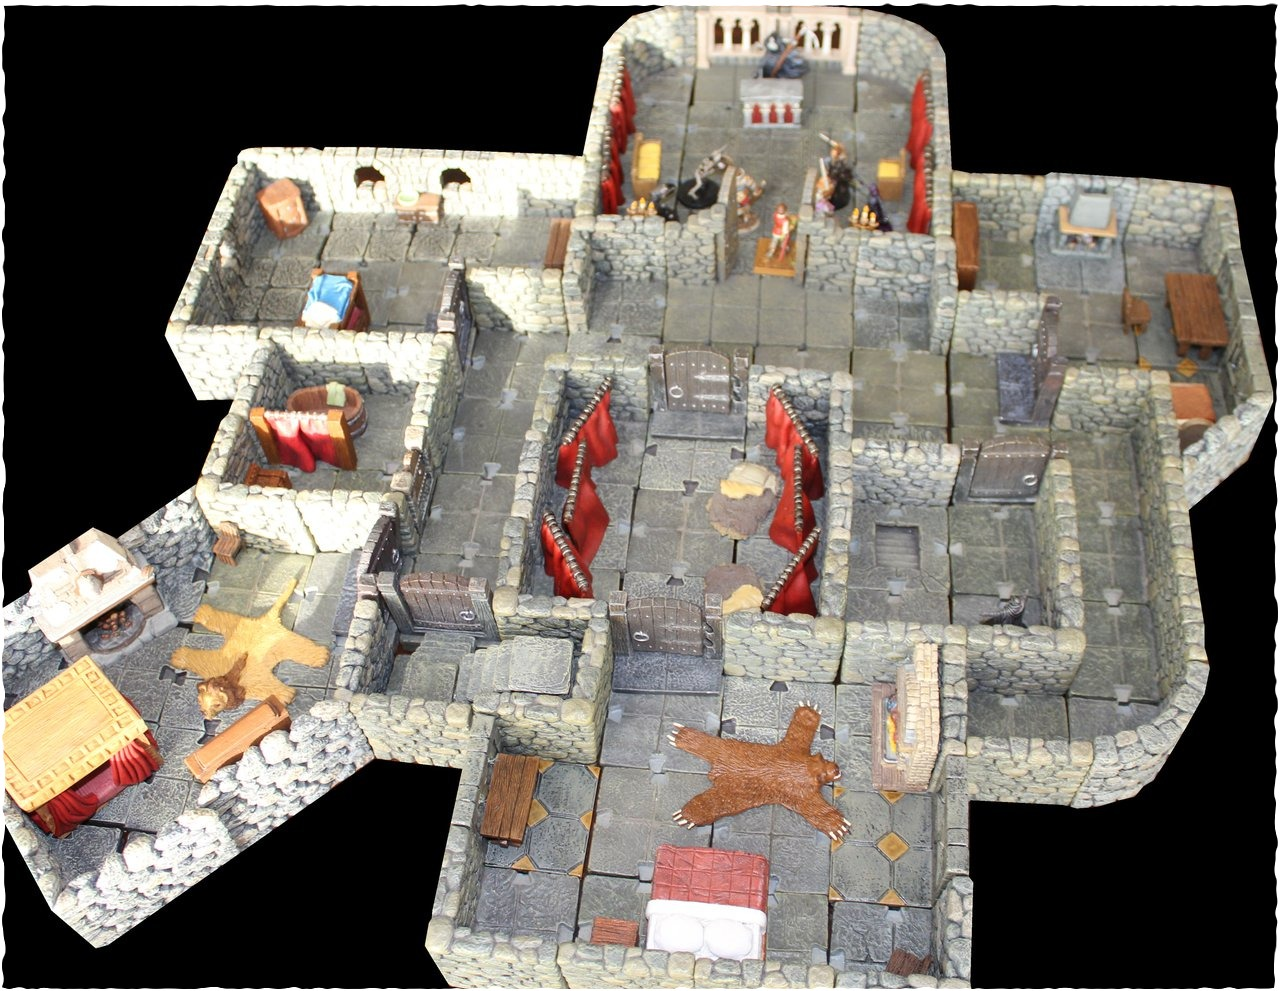
\includegraphics[width=0.4\textwidth]{images/Pathfinder-Foxglove-manor-to-Lost-End-upper-floor-513924264_mod.jpg}
	\caption{Pathfinder Foxglove manor to Lost End upper floor}
	\label{fig:Pathfinder-Foxglove-manor-to-Lost-End-upper-floor-513924264}
\end{figure}

\begin{figure}[h]
	\centering
	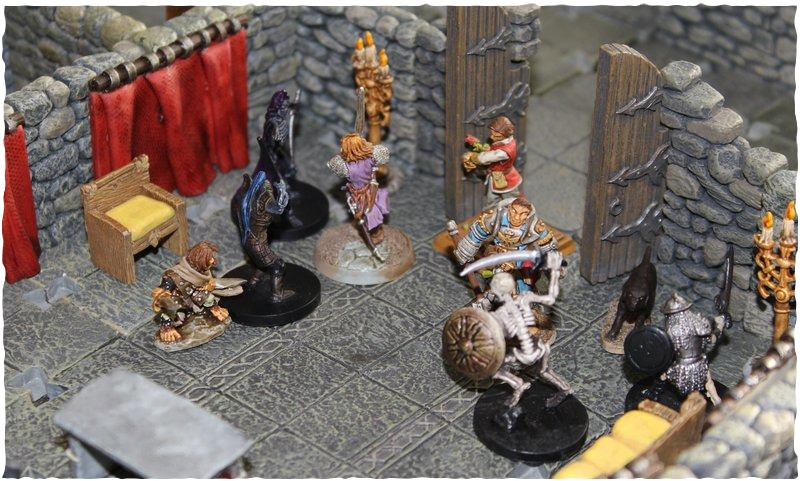
\includegraphics[width=0.4\textwidth]{images/Pathfinder-Foxglove-manor-to-Lost-End-undead-513925444_mod.jpg}
	\caption{Pathfinder Foxglove manor to Lost End undead}
	\label{fig:Pathfinder-Foxglove-manor-to-Lost-End-undead-513925444}
\end{figure}



	%!TEX root = ../crimson_throne_book_main.tex
% 2015-02-15
The companions explore the rest of the upper floor. One bedroom - the size of the bed suggests that this once belonged to a child - was possibly used by Rolth. There are stains of blood on the table and decaying leftover pieces of flesh and hair on the floor. A bloody saw, needle and thread complete the picture of a necromancer's tools for golem crafting. Four other rooms show signs of occupation, a simple bedroom, a portrait gallery with two bedrolls and two master suites. The latter are quite clean: the four-poster bed in one has fresh sheets and smells almost sweet, while the king-sized double bed in the other room has been tidily made up. The drawer in a cabinet holds two very interesting letters.\\

 {\itshape Dear doctor Devils}  We hear you are the man we need, a gentleman-killer who does not strike with physical weapons, but who resorts to more insidious devices like poison and germs. What we need is something between those two: we're looking for a poison that has the symptoms of an ordinary disease, but that cannot be treated with disease fighting magic. The clinical picture has to be realistic enough to make everyone believe that the victim is just ill, while the outcome - let's be very clear about this - has to be fatal! Deliver this and we will make you rich. There might even be more in store for you if you prove successful.\\



	%!TEX root = ../crimson_throne_book_main.tex
% 2015-02-22
The flesh golem roars as it closes in for the attack. The companions are ready for it, though, having read Rotlh's notes. None of them has an adamantine weapon, so they expect to have trouble getting through its thick hide. They do have a very important advantage, however, fire and ice! Sjo can enhance his strikes with flames and Quint's weapon crackles with frost. Both types of magic are supposed to slow the creature.\\

The companions decide to draw the golem into the entrance cave, where they will be able to surround it. Sjo casts a {\itshape burning hands} on it, while he and his friends get into position. The creature follows in slow motion. Quint also prepares by boosting Balian, Sjo and himself with  {\itshape heroism} and Puk sneaks behind the assailant, sneaking through the shadows. The stitched man finally manages to start hostilities, but his first swing goes high and misses Balian completely. The heroes now encircle the creature and strike from all sides, discovering that its resistance to non-adamantine weapons is not as tough as they expected. Instead of the dreaded encounter to the death, the companions find themselves within the grasp of an easy victory. Sure, the golem manages to score a couple of hits, but since fire of ice keep it slowed, it does not pose much of a threat. A few breaths later it topples to the floor. Quint can't get over how easy this was, considering how complicated and expensive it is to create such a being. The heroes\hyperref[fig:Pathfinder-Foxglove-manor-to-Lost-End-cave-515531738]{ explore the caves further } . The tunnel that smells of sea air leads to a huge cave where docks have been built. One big ship could possibly moor here, although it would be treacherous to navigate the water outside the cliffs. It would definitely take an experienced captain to get a vessel into this cave. Along the walls are some left-over supplies, as well as empty barrels and crates. A small prison to the side holds numerous dead rats. \\

\begin{figure}[h]
	\centering
	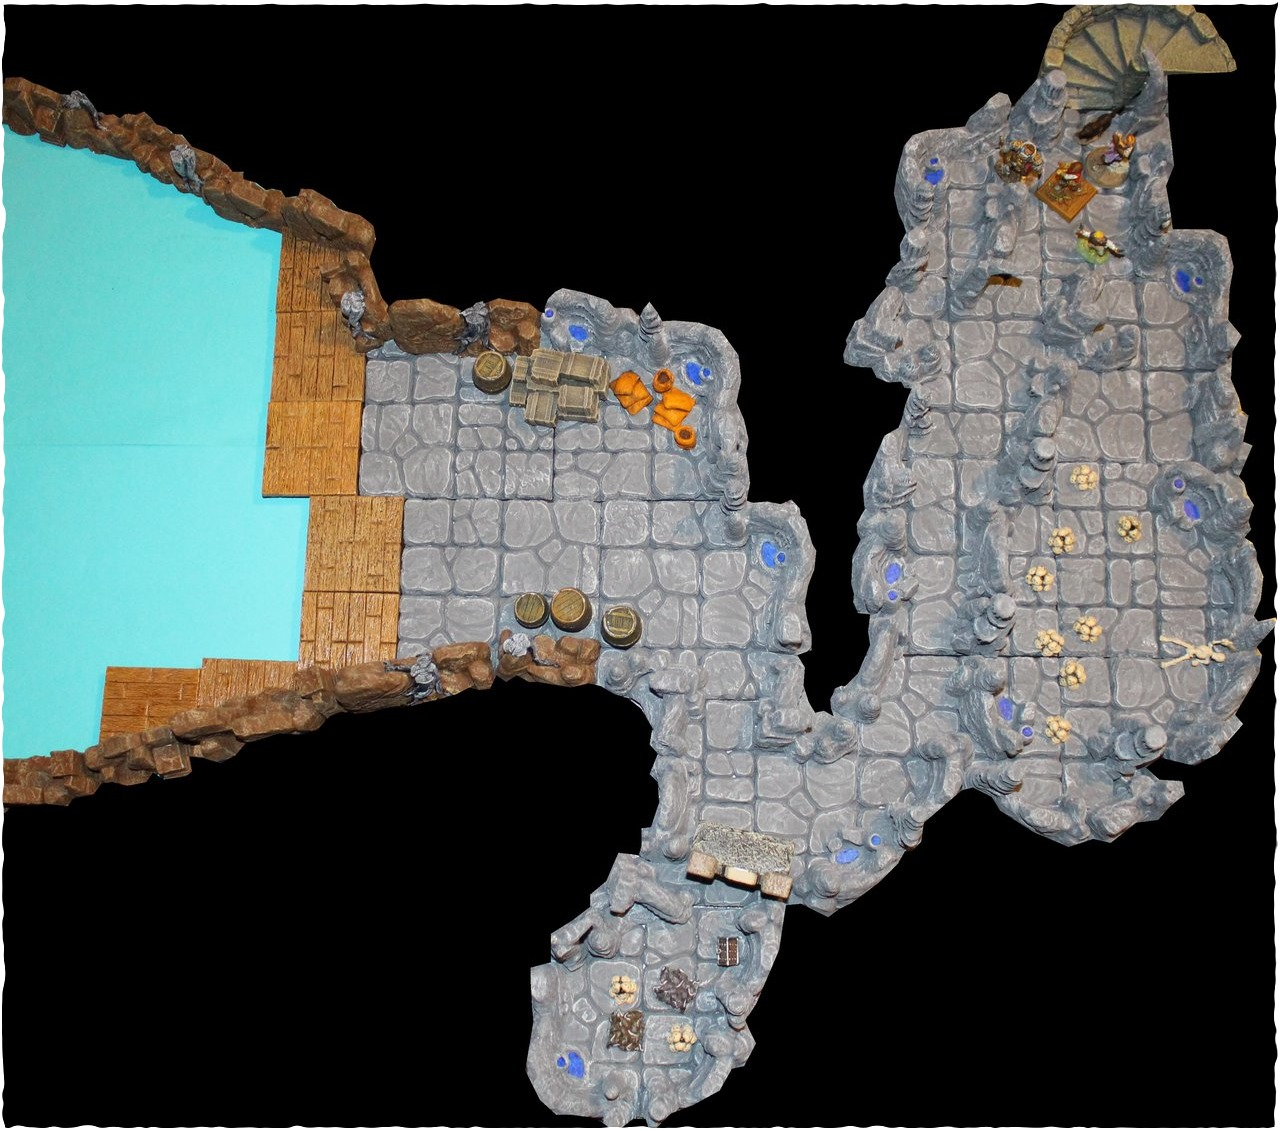
\includegraphics[width=0.4\textwidth]{images/Pathfinder-Foxglove-manor-to-Lost-End-cave-515531738_mod.jpg}
	\caption{Pathfinder Foxglove manor to Lost End cave}
	\label{fig:Pathfinder-Foxglove-manor-to-Lost-End-cave-515531738}
\end{figure}

That leaves only one tunnel, one that reeks of death. With their cloaks in front of their mouths the companions go down the corridor. There is one narrow room at the end that serves as a waste pit filled with hundreds of decaying rodents and a fair number of rotting human corpses. Balian fears that his sister might be one of them, so, despite the overwhelmingly sickening stench, he wants to examine the bodies closer. There turn out to be eleven children here, all girls ... so the lambs that Rolth and the dark-haired lady bought from Gaedran Lamm were sacrificed as guinea pigs! The thought alone leaves the companions foaming at the mouth with anger. Eight corpses are adults, six of which were female as well. Only two had black hair, like Balian's sister, but these two were too old to be Alika. Still, this\hyperref[fig:No-more-mister-Nice-Guy-515533807]{ cruelty will have to be avenged } ! \\

\begin{figure}[h]
	\centering
	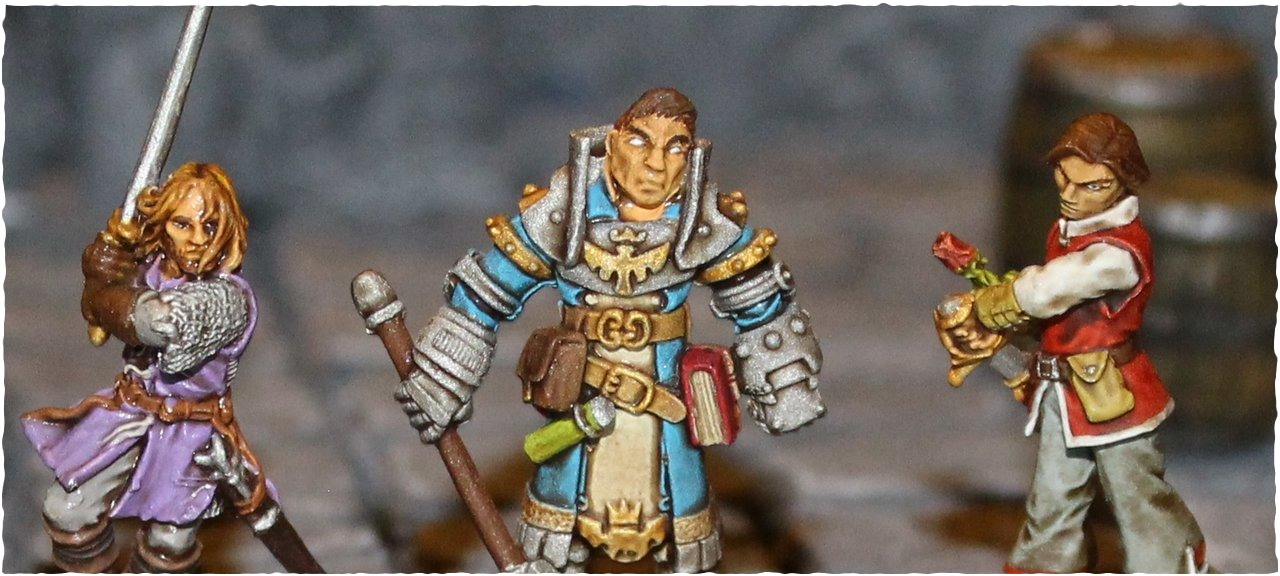
\includegraphics[width=0.4\textwidth]{images/No-more-mister-Nice-Guy-515533807_mod.jpg}
	\caption{No more mister Nice Guy}
	\label{fig:No-more-mister-Nice-Guy-515533807}
\end{figure}

The companions use what is left of the day to make their way back to the Graul hunting lodge, where they spend the night in the barn once again.\\

\section{Level up: level 6!}

\section{5 Erastus 4708}

The companions rise early in the morning and fire their horses on to take them home as fast as possible. They reach the city as the last light slips across the horizon. When they approach Korvosa, they notice two columns of smokes rising from the city: one in the south and another one, more diffused, in the north. Sjo asks a city guard about them. Apparently the number of deaths has increased so much that the Gray District has taken to burning the corpses, explaining the smoke in the south. The fires in the north have another source, though. Since the situation in Old Korvosa has turned so bad, orders have been issued to quarantine the entire district. All the bridges over the Narrows of Saint Alika are being torched, leaving only the one stone bridge, that will be guarded by the Gray Maidens, who will also patrol the shore line to make sure no one sneaks across.\\

The companions decide to look into the situation later tonight. They have been wondering who to trust with the information they gathered in Lost End. Field Marshal Cressida Kroft seems like an obvious choice, but they fear that she will feel obliged to inform the Castle. The queen is still an unclear factor: is she behind this evil or is she an innocent victim? Her behavior at Trinia's trial certainly does not speak to her defense. So that leaves Vencarlo Orisini: the fencing master is definitely on the same side as the companions and his connection to Blackjack, the caped crusader, might prove valuable. Since Vencarlo lives in Old Korvosa, the companions will be able to check out the situation in the north of the city at the same time.\\

First the four young friends head to their villa, to freshen up and have dinner. Madam Nesia and the kids look healthy and they even have a guest: Meep Gildenglare, the old seamstress, is there again. She has taken the liberty of dressing the three boys in smart blue liveries, complete with the pseudodragon symbol and all. Nesia has been doing well, although she admits to sudden bursts of headache from time to time. She still cannot remember anything about her past.\\

After a heartening dinner the companions trek across the city to the stone bridge off Mainshore Boulevard in North Point into Old Korvosa. Upon arriving there, they stumble upon a battlefield. Four score of Gray Maidens have defended the bridge from angry citizens demanding to leave Old Korvosa. At least a hundred of them lie dead on the other bank of the Narrows. It quickly becomes clear that the Queen's guard will not allow anyone across, even if they bear the official seal from Field Marshal Kroft. So informing Vencarlo has suddenly become impossible, unless the heroes try to slip across unnoticed. They decide against it, at least for tonight; too much blood have been spilt already to risk another incident.\\



	%!TEX root = ../crimson_throne_book_main.tex
% 2015-02-22
\section{6 Erastus 4708}

With Madam Nesia in charge of the household things run a lot smoother (and cleaner) at the villa. At breakfast the companions go over their plans for the day. They want to investigate the queen's physicians, to see how far the corruption has spread.\\

They head over to the {\itshape Hospice of the Blessed Maiden} , the warehouse that was turned into the physicians' headquarters. Just as the arrive, they see a patrol with a pair of doctors leaving. Quint casts a  {\itshape detect magic} and notices that both doctors are wearing an enchanted mask. Next the heroes go inside, where they are promptly stopped at the front desk by a burly nurse. The woman is wearing leather gloves and a cloth in front of her mouth. "Get in line!" she shouts, pointing to the six sick people who are already here. A closed door behind the desk provides entry to the main hall, but a Korvosan guard blocks the way. Quint demands to see Doctor Dave Saulus, but the nurse refuses to let him through, until Sjo pulls out the Field Marshal's charter and bullies the woman into agreeing. She leads the companions through the doorway into\hyperref[fig:Hospice-of-the-blessed-maiden-515716825]{ the warehouse's vast interior which has been converted into one gigantic sick ward } . The stench of alcohol and sickness chokes each breath. Rows of stained cots cram the floor, every bed filled with its own pitiful story: men and women of all walks are groaning as the final stages of the plague consume them. The ceiling of the room is nearly 30 feet high, though a series of catwalks span the room at 20 feet. Four dark robed doctors hover amid the sick, their avian masks giving them an unnerving resemblance to crows waiting to be fed. Quint spots magic in each of the facial covers. Four Korvosan guards and one Gray Maiden walk the floor, while three more Gray Maidens patrol the catwalks above. \\

\begin{figure}[h]
	\centering
	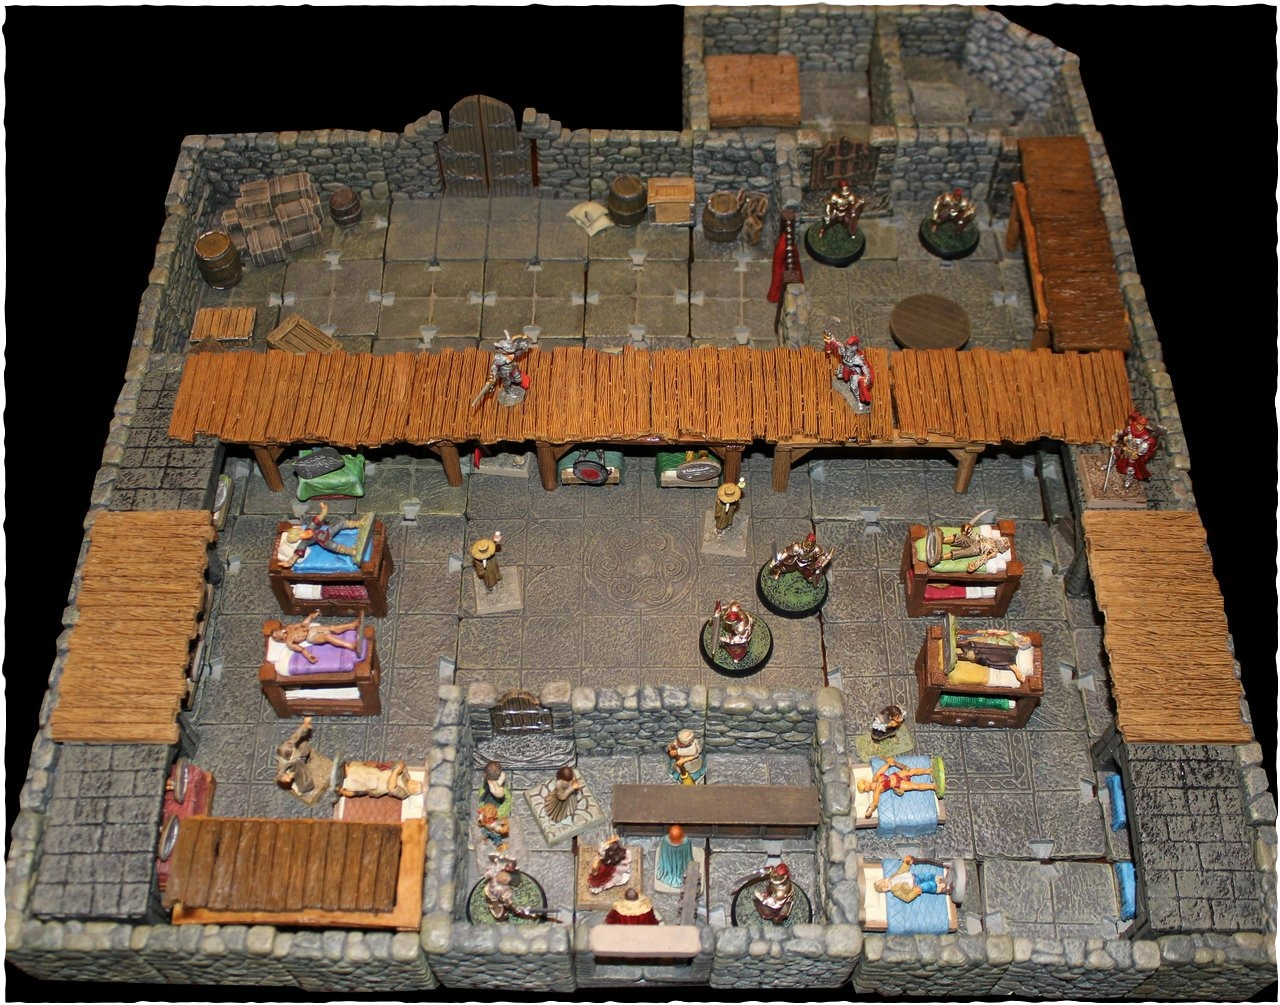
\includegraphics[width=0.4\textwidth]{images/Hospice-of-the-blessed-maiden-515716825_mod.jpg}
	\caption{Hospice of the blessed maiden}
	\label{fig:Hospice-of-the-blessed-maiden-515716825}
\end{figure}

The nurse takes the visitors to a staircase in the back and precedes them to\hyperref[fig:Hospice-of-the-blessed-maiden-upstairs-515717557]{ the fist floor } . There is a second smaller sick room upstairs, in which one of the masked doctors immediately reacts badly to the companions' arrival. Nurse Brunhilde tries to calm the man's protest and urges him to let the guests see Doctor Saulus. During this brief conversation Quint notices that the sick in here are all of Varisian stock, while the doctors are all wearing  {\itshape magic} masks again. Puk spots a leather strap bound to a patient's wrist: these poor wretches have been tied down, possibly for their own safety, but the halfling still feels bad about it. Balian gives one patient a quick look-over and is surprised to see that the man shows no signs of the plague, although he looks sedated. The ranger decides to keep quiet about it for now, but he will definitely have to inform his friends of this later. \\

\begin{figure}[h]
	\centering
	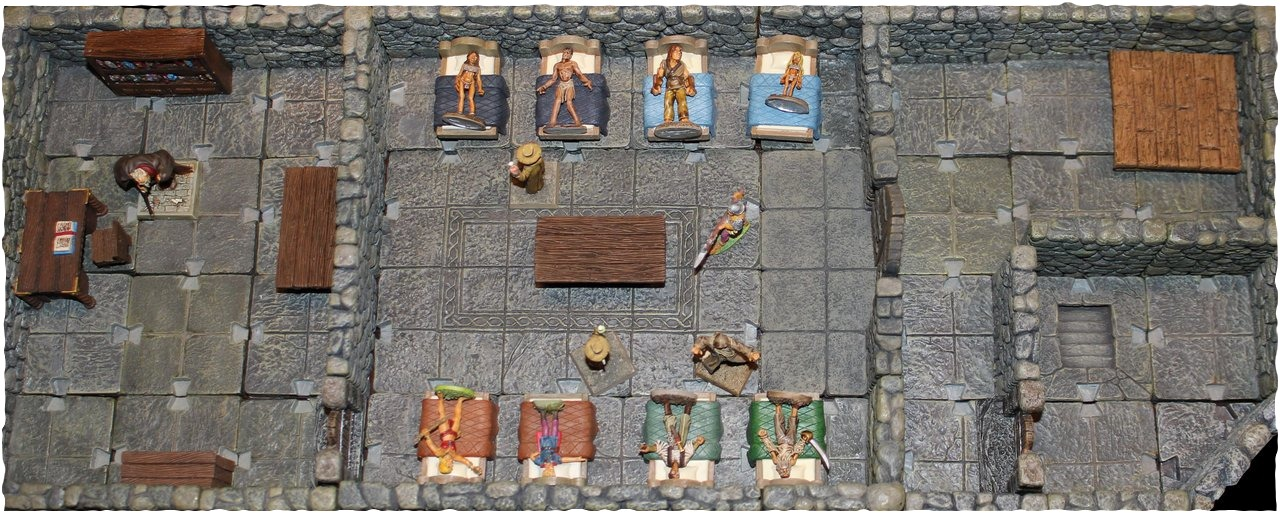
\includegraphics[width=0.4\textwidth]{images/Hospice-of-the-blessed-maiden-upstairs-515717557_mod.jpg}
	\caption{Hospice of the blessed maiden upstairs}
	\label{fig:Hospice-of-the-blessed-maiden-upstairs-515717557}
\end{figure}

Before the protesting physician can utter more objections, Sjo storms through to the back and bursts into the office of doctor Saulus. This time even\hyperref[fig:Hospice-of-the-blessed-maiden-doctor-515717926]{ the head physician is wearing an avian beak over his nose } , which again radiates magic. The companions demand that the doctor gives them an update, but the proud Chelaxian seems very displeased at their sudden arrival and is very curt in his answers. He sees no reason to give any explanation to these annoying upstarts and quickly shows them the door. Puk wants to compare the doctor's handwriting to the plague plan from Lost End and makes an attempt to snatch one of the papers on the table unnoticed. He fails miserably at it, angering the doctor even more, who has the intruders escorted out immediately. \\

\begin{figure}[h]
	\centering
	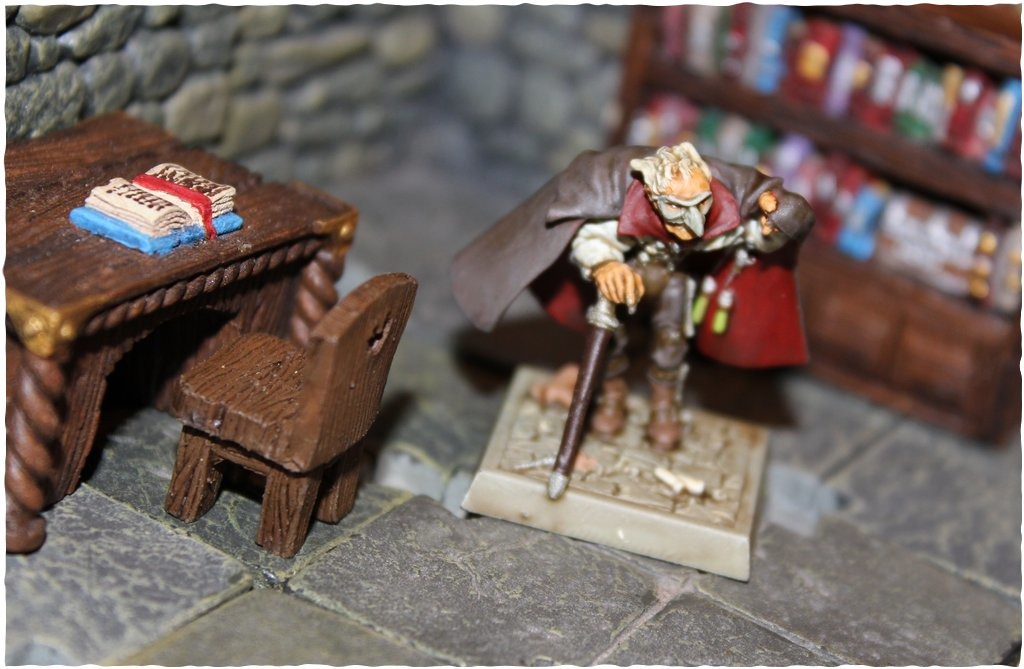
\includegraphics[width=0.4\textwidth]{images/Hospice-of-the-blessed-maiden-doctor-515717926_mod.jpg}
	\caption{Hospice of the blessed maiden doctor}
	\label{fig:Hospice-of-the-blessed-maiden-doctor-515717926}
\end{figure}

The companions contemplate what to do next: Quint wants to kidnap some doctors and force them to talk, but Sjo objects as the recent plague charter explicitly forbids attacking or impersonating the doctors or the Gray Maidens. The lawful healer wants more evidence to legitimize acting against the queen's agents. It might be best to wait for nightfall and sends in Puk to gather more clues. Next the heroes gear up for further adventure by selling off their loot and buying three more wands of {\itshape cure light wounds} . Quint also goes to the library to do research on the Red Mantis, the doctors from Cheliax and Lady Andaisin. He finds no reference to an official medical guild in Cheliax, making him wonder where Ileosa recruited her physicians from. There is no information on Lady Andaisin either, which does not come as a big surprise, since most of the church of Urgathoa consists of underground cults. It makes sense that the names of their high priests remain shrouded in mystery. Another secret organization is the Red Mantis, on which Quint finds only general data. The assassins of the order wear red and black armor with a helmet shaped like a mantis head. It is said that no wall is thick enough, no bodyguard tough enough or no safehouse well enough hidden to keep the Red Mantis from their prey. They take little notice of social or political status, seeing all marks as equal if the client pays the right price. They do refuse, however, to take contracts on rightful monarchs, out of respect for their patron deity, Achaekek, who views monarchs as the earthly parallel of gods. They demand high payment, either in the form of gold or the promise of future collaboration and, once struck, they never go back on a deal. Contacting them is tricky as there are no direct channels to reach them. They is no mention of them ever having been in Korvosa.\\



	%!TEX root = ../crimson_throne_book_main.tex
% 2015-02-23
BALIAN, CG Male Human ranger 6 (urban ranger)  Init Senses  AC touch flat-footed  hp  Fort Ref Will  Speed  Melee  {\itshape greatsword +1} (two handed) +12/+7 ((two handed) 2d6+8/19-20)  Melee  {\itshape masterwork dagger} +12/+7 (1d4+5/19-20)  Ranged  {\itshape masterwork longbow (composite/strength rating+4)} +10/+5 (1d8+4/x3)  Base Atk CMB CMD  Ranger Spells  1st  {\itshape lead blades, longstrider}   Abilities  Special Qualities  Feats  Skills  Possessions  {\itshape greatsword +1} ;  {\itshape ring of protection +1} ;  {\itshape mithral breastplate +1} ;  {\itshape amulet of natural armor +1} ;  {\itshape belt of physical might (+2 str/con)} ;  {\itshape cloak of resistance +1} ;  {\itshape wand of cure light wounds} ; masterwork dagger; masterwork longbow (Composite/Strength Rating+4)  Favored Community Korvosa (Ex)  Favored Enemy (Human +4, Undead +2) (Ex)  Trapfinding (Ex) Trained actor  Child of the Streets  Reactionary SPYDER, dog companion level 6, N Medium animal  Init Senses  AC touch flat-footed  hp  Fort Ref Will  Speed  Melee  Abilities  Base Atk CMB CMD  Feats  Skills  Possessions  {\itshape amulet of natural armor +1}  ---\\

QUINTILIAN, CG Male Human bard 6 (court bard)  Init Senses  AC touch flat-footed  hp  Fort Ref Will  Speed  Melee  {\itshape short sword +1 of frost} +7 (1d6+3+1d6/19-20)  Melee  {\itshape longsword} +6 (1d8+2/19-20)  Melee  {\itshape masterwork whip} +7 (1d3+2)  Melee  {\itshape sap} +6 (1d6+2)  Ranged  {\itshape shortbow} +6 (1d6/x3)  Base Atk CMB CMD  Known Bard Spells  2nd  {\itshape cacophonous call, gallant inspiration, heroism, mirror image}   1st  {\itshape cure light wounds, expeditious retreat, innocence, memory lapse, sleep, timely inspiration, touch of gracelessness}   0th  {\itshape detect magic, ghost sound, light , lullaby, mage hand, message, open/close, prestidigitation, read magic}   Abilities  Feats  Skills  Possessions  {\itshape short sword +1 of frost} ;  {\itshape chain shirt +1} ; masterwork buckler; longsword; masterwork whip; sap;  {\itshape wand of feather step} ;  {\itshape wand of cure light wounds} ;  {\itshape wand of mage armor} ; Shortbow;  {\itshape amulet of natural armor +1} ;  {\itshape Wand of magic missile (CL 3rd)} ;  {\itshape Scrolls of levitate, gentle repose, false life, knock} ;  {\itshape Dust of appearance} ;  {\itshape ring of fire resistance (10)} ;  {\itshape ring of protection +1} ;  {\itshape cloak of resistance +1} ;  {\itshape Key-Lock Killer's bell}  Bardic Performance  Versatile Performance (Comedy / Oratory) (Ex)  Countersong (Su)  Distraction (Su)  Fascinate (Su)  Heraldic Expertise (Ex)  Satire  Mockery (Su) Trained actor  Fast-Talker  Child of the Street ---\\

SHAOBAN (SJO), LN Male Human oracle 6  Init Senses  AC touch flat-footed  hp  Fort Ref Will  Speed  Melee  {\itshape cold iron mace +2 (heavy)} +10 (1d8+5)  Base Atk CMB CMD  Known Oracle Spells  3rd  {\itshape cure serious wounds, dispel magic, fireball}   2nd  {\itshape cure moderate wounds, hold person, resist energy, restoration (lesser), weapon of awe}   1st  {\itshape burning hands, comprehend languages, cure light wounds, magic weapon, protection from chaos, remove fear, shield of faith}   0th  {\itshape create water, detect magic, purify food and drink, read magic, spark, stabilize}   Abilities  Feats  Skills  Possessions  {\itshape cold iron mace +2 (heavy); ring of protection +1; full plate +1; amulet of natural armor +1, cloak of resistance +1, belt of giant strength +2, wand of cure light wounds, wand of remove disease} ; buckler Clouded Vision  Flame Mysteries  Touch of Flame (Su)   Molten Skin (Ex) Trained actor  Child of the Streets  Ease of Faith 

	%!TEX root = ../crimson_throne_book_main.tex
% 2015-02-26
PUK, CG Male Halfling rogue 6 (swashbuckler)  Init Senses  AC touch flat-footed  hp  Fort Ref Will  Speed  Melee  {\itshape silver short sword +2 (small)} +11 (1d4+2/19-20) and off-hand  {\itshape masterwork short sword (small)} +10 (1d4/19-20)  Melee  {\itshape masterwork sap (small)} +12 (1d4 non-lethal/x2)  Ranged  Ranged  Base Atk CMB CMD  Atk Options  Abilities  Feats  Skills  Possessions  {\itshape small silver short sword +2} ;  {\itshape studded leather +2 (small)} ; Shortbow (Small); Halfling Sling Staff (Halfling); small masterwork sap,  {\itshape amulet of natural armor +1} ,  {\itshape ring of protection +1}  Sneak Attack (Ex)  Bleeding Attack (Ex) Fast-Talker  Personal Addiction 

	%!TEX root = ../crimson_throne_book_main.tex
% 2015-02-28
The young heroes of Korvosa keep an eye on the Hospice of the Blessed Maiden for the rest of the day. In the evening all the doctors who have been patrolling the city return. While the guards accompanying them leave after a few minutes for their barracks, the physicians themselves do not come out of the warehouse again. So they must have their own sleeping quarters in the building, possibly in the backroom, which the companions haven't seen yet. Most doctors also bring some new patients with them, who will probably occupy the beds of the dozen cadavers that are carried off by body carters before the sun sets. However, no patient has left the Hospice alive or cured today.\\

The companions wait for darkness before attempting to break in. Their goal is to get Puk into Doctor Saulus' office to compare his handwriting to the plague plan notes they found in Lost End. The huge backdoor to the Hospice is unguarded. Puk puts his keen ear to the wood and hears nothing on the other side. If a dozen doctors are staying in there, they must either be very quiet or already fast asleep. The halfling also fails to see any light coming through the cracks of the door. He feels quite comfortable that there is no one in there, at least not awake. The door is barred, so Quint uses his magic bell to open it. When no reaction comes to the bar dropping on the ground, Puk looks inside: this backroom is an unlit loading bay that is filled with empty crates, containers and barrels, the remnants of the Arkona venture that occupied this building in the past. Two curtains lead to the main hall. Puk slips in the backroom and peeks under the heavy drapes into the sick ward. There are two doctors left to look after the patients and a pair of Korvosan guards plus three Gray Maidens to provide security. The halfling informs his friends outside. Quint hopes that things in the ward will get even quieter (and hopefully even less crowded) in the middle of the night, so the young men decide to come back after midnight.\\

\section{7 Erastus 4708}

The companions return after a couple of hours. The backdoor is still open, so Puk slips back into the loading area. The number of guards and doctors in the sick ward hasn't changed, but the two doctors are no longer among the patients' beds, they have taken a seat at a table in the back instead. Damn, now they are effectively blocking Puk's path to the stairs! The halfling quietly calls over Quint, who might be able to draw the physicians back into the main area with a {\itshape ghost sound} spell. Unfortunately, the bard stumbles into one of the crates in the unlit loading bay: "THUCK!". He does not hesitate and quickly runs out again, pushing the door shut behind him. Puk tries to hide behind a container as one of the Gray Maidens pulls away the curtain and peers into the backroom. Lighting her way with a flickering torch, she walks over to Puk's hiding place and discovers the little rogue in the corner with a sheepish smile on his face. "Who are you? Get out of there!" the woman orders. Puk stands up and shrugs, but then jumps between the lady's legs and bolts for the backdoor, which his friends open from the outside. The Gray Maiden pursues him and suddenly finds herself facing four men instead of one.\\

"We are the pseudodragons, heroes of the city, and we're here on official business", Quint tries.\\

"Official business my ass! ALARM! I'm giving you one chance only, lay down your arms, NOW!" the woman cries as she holds out her blade threateningly. She quickly gets the company of her two colleagues, the two Korvosan guards and one plague doctor. One of the other Gray Maidens is clearly an officer, who immediately takes command. Quint and Sjo pull out Kroft's charter and wave it in her face, claiming they are here to examine potential treason by the queen's physicians.\\

"If you are sent by the Guard, you are under our orders as well, since we are in charge of all military forces in the city now", the officer throws back.\\

"Well, we're not actually with the Guard as such, so we're not really taking orders from anyone, but we are on the same side", Quint replies. "You see, I know that you are loyal to her majesty, the magnificent Ileosa. But I fear that both her majesty and you are being misled by darker forces, forces we should actually fight together." Resorting to his powers of bardic persuasion Quint tries to fascinate the commander and the Gray Maiden who discovered Puk with his words. He is obviously successful, as she relaxes her stance and seems prepared to listen to him. "Maybe I might even {\itshape suggest} that you help us", Quint tries, attempting to pull the officer further in his charming ploy, but she resists his wiles now. Puk, Sjo and Balian feel the tension dropping and take advantage of the moment to bid the mesmerized guards goodnight, slipping away around the corner. Realizing that he will not be able to get this Gray Maiden to cooperate with his plans, Quint changes his tactics now. "I guess it was all just an {\itshape innocent} mistake, I see that now", Quint continues, activating his  {\itshape innocence} spell to boost his bluff. "We were clearly mistaken, I apologize for disrupting you. You're doing an excellent job, by the way, keep up the good work! I'm sorry again for the misunderstanding, I'll just take my leave now." The bard slowly walks backwards to the corner of the warehouse while sweet talking the guards. Then he slips around the building as well, leaving the stupefied security at the backdoor. That was close! This was the first time in my long roleplaying career that I actually saw the bardic powers of persuasion being put to full use. We usually have a bard in our parties who makes ample use of skill in 

	%!TEX root = ../crimson_throne_book_main.tex
% 2015-02-28
The companions wait fifteen minutes before returning to the warehouse. It looks like two Korvosan Guards are now patrolling the building on the outside. Quint, Puk and Balian wait for them to pass, before climbing up the wall to the roof. They make their way over the rooftop to the front of the building, above the office of Doctor Saulus. Puk keeps watch while Balian quietly pries away some of the wooden boards that cover the top of the building. A few moments later Quint and Puk slips into the doctor's workplace. Quint summons some light and goes over the writings on the desk. He puts the plague plan from Lost End next to them and compares the handwriting. There is no mistake: the same curls on the l's, the same 'dots' (or rather small lines) on the i's, and the same slant to the letters. In a drawer the bard also discovers a document that discusses the immunity to the plague in a certain part of the Varisian population, despite various attempts and experiments to get them sick. Then Quint's eye falls on a document with the doctor's name on it. Some letters stand out in the dim lightD v l s The office connects to the smaller upstairs {\itshape sick} ward, in which the patients weren't really sick, as Balian discovered earlier on. These must be the immune Varisian guinea pigs on which Saulus has been experimenting. Puk listens and hears one man walking around in the room. Balian joins his friends and draws his greatsword, while Quint signals to him that the enemy has to be taken alive. Puk pushes the handle down and clicks the door open, before slipping back in the dark corner. From inside the small sick ward he hears footsteps coming closer. A masked doctor stands off against the light in the background as he pushes open the door and peers into the dark of the office. Quint surprises the man with a {\itshape cacophonous call} , while Balian jumps up and hits him hard on the head with the pommel of his sword. The physician drops to the floor, unconscious. The patients in the room beyond do not react to this disturbance, they have obviously been drugged. The companions carry out the doctor, rejoin Sjo and make for the old fishery with their unconscious prisoner. They strip him of his clothes and discover a lot of strange vials and even a formula book in his leather coat. So, this man is an alchemist who uses chemistry to do his magic. Sjo throws a bucket of water in the man's face to wake him up, alchemy for beginners, lesson one.\\

At first the prisoner will only give up his name, Lennerd Brand. For the rest he feigns innocence. "We're here to help the people, that's all."\\

"Not a lot of help you are, then. I only saw dead leaving the hospital. Aren't you supposed to cure the sick? Well, I guess that is not what good old doctor Devils prescribes, is it?" Sjo spits.\\

"I can't help it that those people are just too far gone to be saved. We do our best. It's not like doctor Devils can perform miracles ... eh ... doctor Saulus, I mean."\\

"Haha, you stupid Urgathoan scum, nothing like a slip of the tongue to get to the truth", Sjo smiles as he burns the man in the leg with his power over fire. "Now spill the beans or suffer the consequences of your lies!"\\

"Here's the truth for you, you ignorant fool! Urgathoa's wrath will burn you all!" the doctor now scream madly.\\

"The only one who'll be burning with Urgathoa is you. Tell me, do you also dance around on skeletal legs in the afterlife when you're an Urgathoa hugger?" Sjo mocks.\\

"Just know that I'll be using these legs to dance on your eternally tortured soul. I give my life willingly to the Pallid Princess! She'll reserve a place of honor in her realm when I arrive after all we've achieved in this backwater city. Seldom has the queen of disease been served so well! Our success here will be the stuff of legends!" the doctor laughs.\\

"Tell us about your plans!"\\

"Never, I'll die before helping you."\\

"Well, I wouldn't say you'd have to die, that would be terribly inconvenient for both of us. Wouldn't you rather tell me all about the glory of Urgathoa right now?" Quint intervenes as he spins his verbal web of {\itshape fascination} again. The glare in the doctor's eyes tells him he is successful. "Now, if I can be so bold as to make a  {\itshape suggestion} , why don't you tell me what you know about Doctor Devil's plans." This time Quint's suggestion takes hold and the captured physician confesses: "Well, we arrived on that ship, the Delivery, but we got off before we reached the city, all except Rois. He was chosen as Urgathoa's champion, to sink the boat in the river mouth. We made it to shore and revealed ourselves a couple of days later as the 'doctors' who were supposed to fight the plague. We had to pretend that someone from Cheliax had teleported us in, you know, to explain how we got here so fast."\\

"And who are you working for?"\\

"I don't know, we get our orders from Doctor Devils and ... Lady Andaisin." The tone in the man's voice betrays that he is in awe of Urgathoa's highpriest.\\

"And where is she right now? Where are all of the doctor, actually?" Quint asks.\\

"There is a secret basement below the warehouse, if you switch a lever in the lift, it can take you down to our new temple! They say that this underground complex was used for smuggling in the past. The former owner of the building was none too happy when he had to give it up, {\itshape Arkomer} or something he was called. Anyway, that's where my brothers and sisters are, as is Lady Andaisin." "And what are you doing to those patients, especially the Varisian ones on the first floor?"\\

"It turns out that some Varisians are immune, we've been trying to find out how to get them sick, but nothing has worked so far. They are probably too stupid to realize that they should get sick, huhu, even rats know better", Lennerd replies with a cocky smile on his face as he stares at Balian. "Like that dimwit with the big sword, looks as stupid, but also as healthy as a horse."\\

Balian can't control himself and smacks the man in the head: "That will wipe that smirk of your face!" Unfortunately his aggressive action snaps the doctor out of Quint's suggestion. As it sinks in that he just gave away so many secrets, the man's face turns bitter. "What foul trickery did you throw over me? You will get no more answers out of me! Urgathoa damn you all to eternal hunger!"\\

"We have all we need from you, mister Brand. We'll be sure to tell your friends how cooperative you were. I'm sure they'll appreciate it", Sjo nods. "We'll be back for you later." At that Puk saps the man on the head, knocking him out again.\\

With only two to three hours left before sunrise, the companions know that they have to act quickly. Come morning, the physicians in the Hospice will discover that Saulus' office was broken into and that one of their own is missing. It will not be hard to link this break-in to the pseudodragon 'heroes' who were hanging around the backdoor earlier tonight. If they don't act immediately, the companions might have red Mantis assassins on their tails tomorrow. If there is still some element of surprise left, it is now!\\

Quint puts on the doctor's coat, hat and mask to make him look like one of the physicians. Sjo no longer objects to breaking the royal decree on this point, obviously the doctors are guilty of a worse crime: spreading the disease purposefully. The four heroes return to the warehouse. If they can bypass the ground floor, they will not have to face any innocent Korvosan guards or Gray Maidens. Not unless some of them are down in the underground temple as well, but then they won't be able to claim innocence anymore. Using the hole in the roof, the companions get back to the office on the first floor. Across from the sick room is the wooden elevator. Puk examines it and finds the switch that the doctor told them about. Pulling the ropes ever so quietly, Balian slowly descends the platform into the basement.\\

The way off the platform is blocked by a door. Puk listens at it but hears nothing. Time for some serious action! Then he\hyperref[fig:Entering-the-Temple-of-Urgathoa-516987053]{ pushes the door open } . \\

\begin{figure}[h]
	\centering
	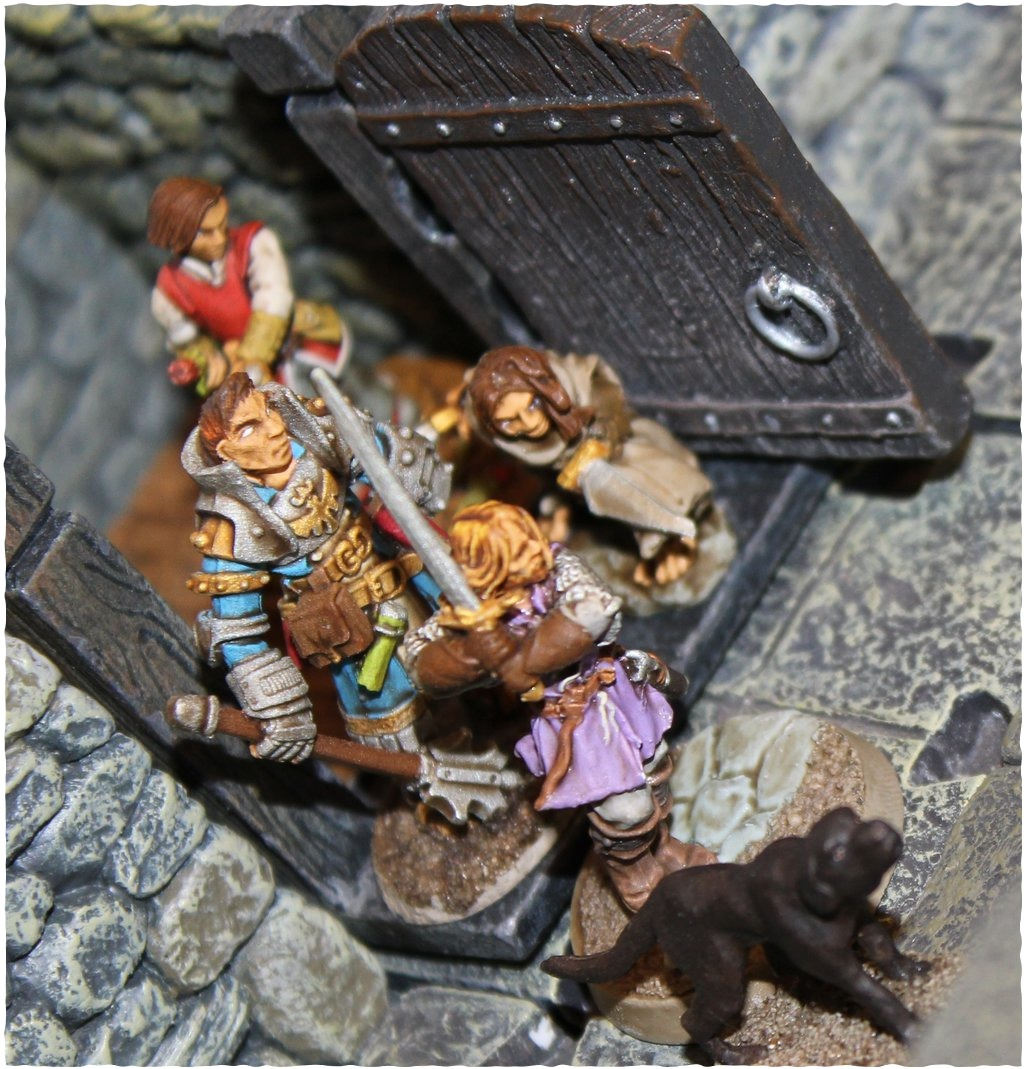
\includegraphics[width=0.4\textwidth]{images/Entering-the-Temple-of-Urgathoa-516987053_mod.jpg}
	\caption{Entering the Temple of Urgathoa}
	\label{fig:Entering-the-Temple-of-Urgathoa-516987053}
\end{figure}



	%!TEX root = ../crimson_throne_book_main.tex
% 2015-03-01
I realize I never put up pictures with an overview of the Graul family homestead, so here they are:  

	%!TEX root = ../crimson_throne_book_main.tex
% 2015-03-14
Before the companions lies what looks like the entry hall to the secret hide-out underneath the Hospice of the Blessed Maiden. The hall sits empty and seems recently redecorated with murals of skeletons feasting among the dead and diseased citizens of Korvosa. The paintings are crudely done and have already been damaged by water seepage from the surrounding rocks. Simple wooden doors lead in every direction, each bearing a painted scythe-wielding skeleton.\\

Puk and Balian sneak in and listen at the doors. They only pick up something at the one on the right-hand side: people snoring inside! Fantastic! So they still have the element of surprise on their side. The urban ranger and the rogue quietly open the door and find four of the queen's physicians asleep in a small storage room. They waste no time and murder the men in their sleep. Quint is content to learn that his {\itshape principled} friend Sjo has no qualms about these merciless assassination tactics, after all, the physicians' guilt has been clearly established. This is swift and clean justice! The companions now try the left door in the entry hall, which leads to a cloakroom. Two big wardrobes hold several dark leather robes, high boots, wide-brimmed hats and beaked plague masks. Sjo also discovers some {\itshape potions of cure moderate wounds} and a bag with 23 black onyx gems, worth 50 GP each, stuck away behind the robes. There is another door in this room which again reveals the sound of people sleeping on the other side. Quint, who is still wearing the avian mask and leather coat as a disguise, walks in first to find a room filled with cots: there are no less than ten physicians resting in here. As Balian and Puk sneak inside to quietly end these bastards' lives, one of the sleepers stirs and sits up. Quint walks over and tries to set his mind at ease with some casual conversation while his friends slip into position to strike the man down in his bed. The plan works, but the noise seems to have awoken another doctor. Again the companions act fast and kill him before he can raise the alarm. The rest of the sleeping doctors are put to the sword as well. The companions continue their exploration by returning to the central axis of the hide-out. They discover a\hyperref[fig:Bacchanal-of-Urgathoa-beneath-the-Hospice-520054146 ]{ chamber with a dozen skeletons lining the walls } . Their bony fingers claw in the air and the empty sockets in their skulls stare at the intruders with nightmarish determination. Sjo immediately reaches for his mace, but then he sees that the bones do not move. It seems like some twisted mind set them on display here in a  {\itshape tableau mort} , to remind all the living that they will one day die and their remains might be called upon to serve the Pallid Princess. Urgathoans certainly have a weird concept of art, no wonder they have to hide it under the ground. A heavy, metal door leads deeper into the complex, probably to the temple itself, but the companions leave it for now, deciding to veer off to the right first because they hear voices coming from that side. \\

\begin{figure}[h]
	\centering
	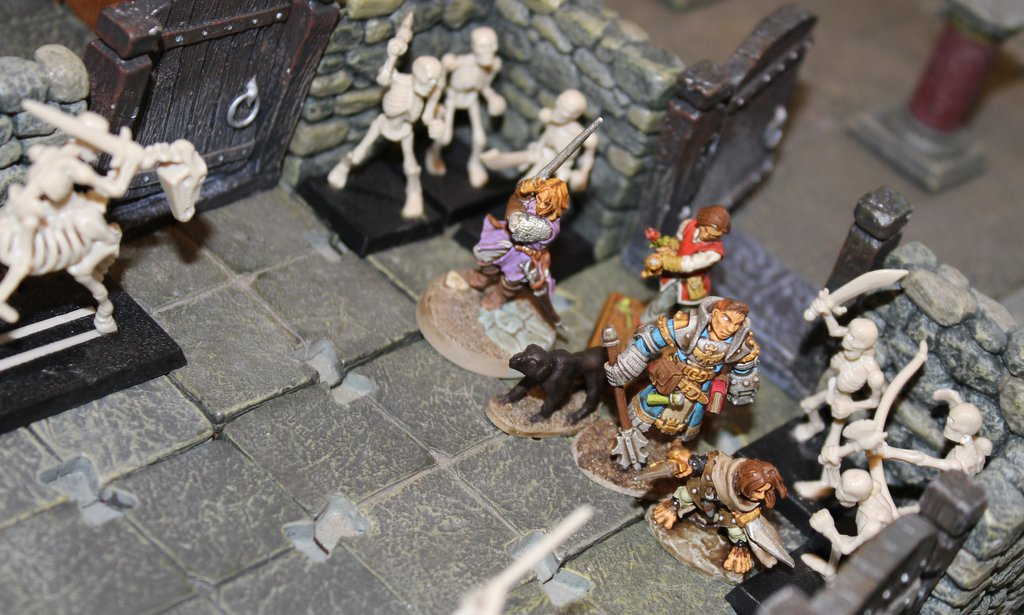
\includegraphics[width=0.39\textwidth]{images/Bacchanal-of-Urgathoa-beneath-the-Hospice-520054146 .jpg}
	\caption{Bacchanal of Urgathoa beneath the Hospice}
	\label{fig:Bacchanal-of-Urgathoa-beneath-the-Hospice-520054146 }
\end{figure}

Balian picks up an agitated voice through the door. "I tell you again, I'm sorry for disturbing your rest, but there were some fierce-looking guys snooping around upstairs. I know you want to be informed of anything suspicious happening; they were talking about about investigating this place before they suddenly made off, spilling some sorry excuse of having made a mistake. I didn't trust them one bit, but that Gray Maiden officer seemed to believe them and let them go. I discussed it with Sordek upstairs and we finally decided it best to inform you. Better to be safe than sorry, right?"\\

Quint decides to go in first again, making use of his disguise. Swinging open the door he walks into another bedroom with six people, all awake and fully dressed: doctor Saulus, a masked physician, two cultists in a breastplate carrying a scythe, a pale and skinny man, with a blotchy and scarred face, and a dark-haired woman. Quint immediately recognizes the gaunt individual as Rolth, the necromancer, the villain they have been trying to track down for ages. The woman in his company must be the lady who took away all those girls from Gaedran Lamm; the girls they discovered later in the mass grave underneath Lost End, where they had been used as guinea pigs for the plague. The bard still feels sick thinking about it. Still, the black-haired lady looks quite young herself, certainly no older than sixteen or seventeen. In fact, she looks familiar as well ... By the gods, could it be? Is Rolth's black-haired accomplice Balian's sister Alika? Quint tries to swallow down the shock that clumps his throat and tries to catch his bearings as Saulus addresses him: "So, any news from upstairs? Did you see those men again that Geoff here told us about?"\\

"Uhmm, no sir, all's quiet, nothing to report", Quint replies.\\

"Well, we might as well check it out, we're up anyway", Saulus responds as he signals the two cultists to lead the way. While Quint slips deeper into the room to the woman's side, the first cultist walks out of the room, only to be surprised by Balian and Puk, who promptly cut him down. Geoff, the physician who came down to warn Saulus, quickly quaffs a vial and peeks around the corner to see who just killed his cultist buddy. "You see, I told you, it's them, it's them!" he cries.\\

Quint sticks to his role and grabs the lady's arm: "By the gods, intruders! Do you have a weapon for me, {\itshape Alika} ?" In spite of his desire to see it otherwise, the black-haired woman responds to the name  {\itshape Alika} . "Here, take one of my daggers." Balian, who rushes in with Puk to finish the other cultist, picks up the name as well, realizing that he is now facing his sister. He immediately tries to reason with her: "Alika, it's me, Balian, your brother. We've come to free you!"\\

"Huh, my brother to the rescue? After five years? You're nothing but a coward and traitor, and a fool! I have found my true purpose in the service of Urgathoa! Now face her and my wrath!"\\

Meanwhile Saulus and Rolth retreat to the far end of the room and cast defensive spells, as Sjo appears in the door opening and throws his new spell on them, {\itshape fireball} ! Spyder also springs into the chamber, but when he recognizes Alika's scent, \hyperref[fig:Spyder-recognizes-Balian-s-sister-Alika-520054718]{ he starts wagging his tail } . The masked physician pulls out another vial and flings it at Balian: it explodes in a burst of flames. Quint uses his disguise one final time in this combat, to take position at Rolth's side. Then the bard pulls out his sword and hacks away at the necromancer. His blade hits the skin as if it was stone. Darn, he just cast  {\itshape stoneskin} ! Doctor Saulus mutters the words of another spell, trying to  {\itshape slow} Balian, Puk, Spyder and Sjo, but the magic only takes on the dog and the halfling. Alika also moves over and viciously cuts at the slowed rogue, proving to have similar skills in combat with her sneak attack. Rolth realizes the threat the 'physician' at his side poses and steps back, flinging two  {\itshape scorching rays} at the disguised bard. Now it is Quint's turn to smile, because he has an effective magical defense of his own: his ring of fire resistance absorbs the burning damage. Sjo charges to the bard's side and engages Saulus: his heavy mace hits the doctor hard! Balian's greatsword swings even harder on the physician who tries to escape his reach to do another spell, but the ranger  {\itshape steps up} and kills him with one clean stroke. Next he joins his friends in the corner to fight the two powerful mages. His hatred guides his blade at the necromancer, but his anger clouds his combat savvy and he misses the foul caster. Doctor Saulus clearly feels outmatched and tries to swing the balance in his favor by casting  {\itshape improved invisibility} on himself. Sjo and Quint hear him running off and chase after him. Sjo throws a sheet of fire in front of him and the flames of his  {\itshape burning hands} reveal the shape of Saulus. Quint snatches some  {\itshape dust of appearance} from his pocket and blows it in the same direction, breaking the doctor's concealing magic. Still, doctor 'Devils' proves worthy of his nickname when he steps back and calls down the fires of hell! A mighty fireball turns the room into an inferno, but when the licking flames burn out, only Puk and Alika have been badly hurt. Quint and Sjo dodge most of the blaze and their protection from fire wards them from most of the remaining damage. \\

\begin{figure}[h]
	\centering
	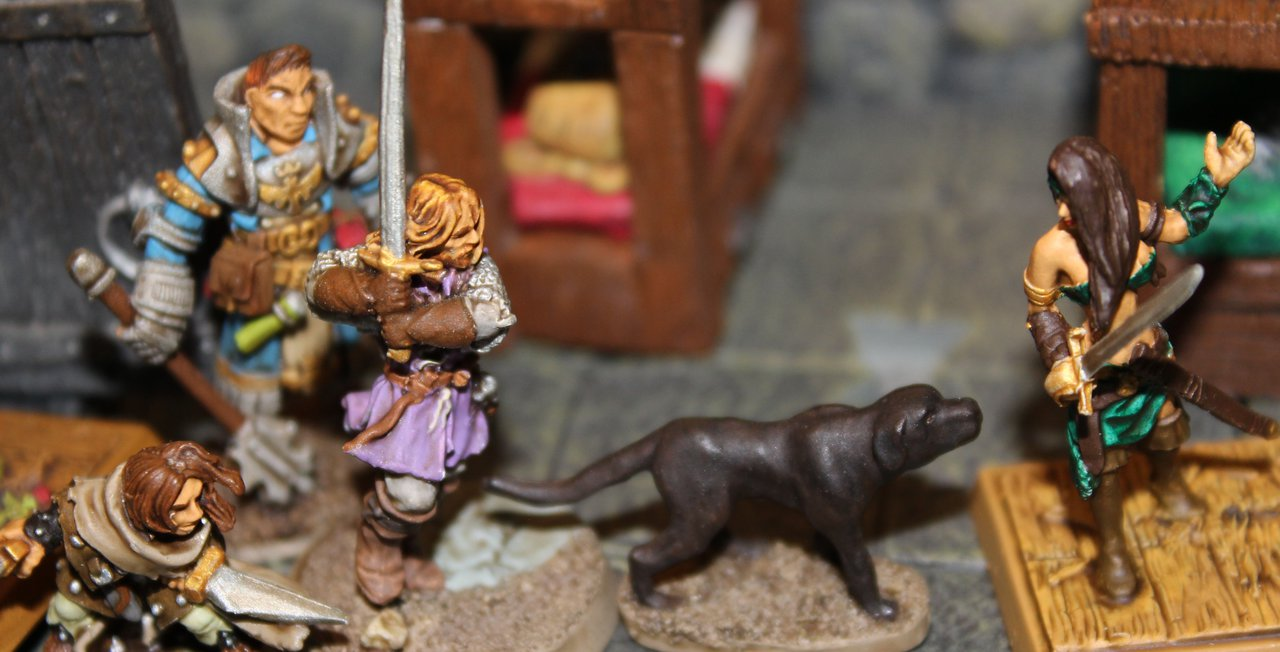
\includegraphics[width=0.39\textwidth]{images/Spyder-recognizes-Balian-s-sister-Alika-520054718.jpg}
	\caption{Spyder recognizes Balian's sister Alika}
	\label{fig:Spyder-recognizes-Balian-s-sister-Alika-520054718}
\end{figure}

The odds are now clearly in favor of the companions: Balian controls his rage and hits down Rolth with the flat side of his blade. Quint and Sjo mock Saulus's feeble attempts at hurting them and cut off his escape route? With Balian's help they knock out the doctor as well.\\

Now only Alika remains. Sjo freezes her in place with a {\itshape hold person} , giving Balian the chance to disarm and bind her before she can move again. So, how does this work? How do you talk to your sister after she has tried to kill you? Especially when you're out of practice with the concepts of brotherly love as Balian is ... 

	%!TEX root = ../crimson_throne_book_main.tex
% 2015-03-28
Finally ... finally ... With a mixture of relief and sadness Balian tries to come to grips with what just happened. Yes, after five years he has finally found his sister; after five years he has finally tracked down the bastard who took his dear Alika from him and yes ... the foul kidnapper did not get away. But half a decade is a long time, the vicious necromancer got under her skin, he brainwashed her, changed her, molded her into his equally vicious right-hand woman. Looking at her now, as she's being bound and gagged, Balian sees nothing but hatred in her eyes. Only Spyder treats her as if nothing has changed, clinging to her side and rubbing his head against her leg. The ranger calls his dog over. The animal gives him a sad puppy look, quickly licks Alika's hand before hesitantly trotting to his master's feet.\\

Puk finds a key ring with a set of heavy keys next to the door in the back of the room. It opens into a small cellblock, which still holds three prisoners. One of them is dead, one unconscious and one barely alive. All three display heavy symptoms of the plague. Sjo offers the two living ones, a boy and a young woman, a {\itshape lesser restoration} to restore some of their stamina. The boy recognizes the healer, he is a stable boy from the Great Tower, the headquarters of the Sable Company, where Sjo used to work as well. His name is Dalvun. He explains that he and his other cellmates have been used in experiments, they were frequently made to drink foul water by Doctor Saulus, Rolth, Alika and Lady Andaisin. Most of them are dead now. Only he and Jaelle are still alive. The two survivors are told to wait in the cultists' barracks, while the unconscious enemies are locked behind bars now. Sjo tells Dalvun he will be back soon, but first he and his friends have to take care of the evil priestess. Returning to the room with the skeletal bacchanal of Urgathoa decorating the walls, the companions now take the heavy metal door deeper into the complex. The stinging scent of chemicals greets them. A huge basin, filled to the brim with foul, murky water, dominates the center of this high-ceilinged chamber. Two sets of stairs to the left and right lead to a catwalk ten feet above the ground which stretches over the pool. Two cultists are inside, one of them stands at the back of the room in an open door. "Warn our Lady that the intruders have arrived!" he yells to someone in the room beyond, before shutting the door. The other cultist is up on the catwalk. Puk, Spyder and Sjo make quick work of the first one, while Balian storms up the stairs and engages the cultist on the overpass. His heavy blade sinks deep into the poor man's shoulder. The ranger pulls his sword free and cleaves the Urgathoan devotee in two: his legs drop down on the metal walkway, while his torso plummets in the foul water below. A fitting end for one who worships a goddess whose upper and lower body are so distinctly separated.\\

The companions decide not to waste any time and ignore the doors to the left and right for now, choosing to follow the shouted warning and explore the way ahead first. The door opens into a hall with four large, cylindrical glass vats, each filled with a bubbling emerald fluid that tints the chamber's light a noxious green. Within each container floats a malformed abomination - part man and part horse - a lean, leathery male body resting on a horse's hind legs and topped with a fleshless equine skull. Three of these forms drift motionless in the green bile, but the fourth still twitches. An alarmed cultist is standing next to the fourth vat and smashes the glass to pieces, spilling the vile liquid over the floor and freeing the creature within. Balian and Puk charge the man and cut him down, but are greeted by the abomination, which lowers its jaw bone, spreading its mouth wide: a swarm of corpse-bloated black flies spills forth from its beak, biting and sickening the two unfortunates. Quint and Sjo resort to combat healing to keep their mates afoot, while\hyperref[fig:Leukodaemon-523050841]{ the daemon now starts clawing and chawing at all those within its reach } . The companions lure the creature away from the corner, so they can surround it and start cutting it up one gash at a time. Their combined attacks quickly outpace the creature's offensive and a few moments later the giant harbinger of disease lies dead at their feet. \\

\begin{figure}[h]
	\centering
	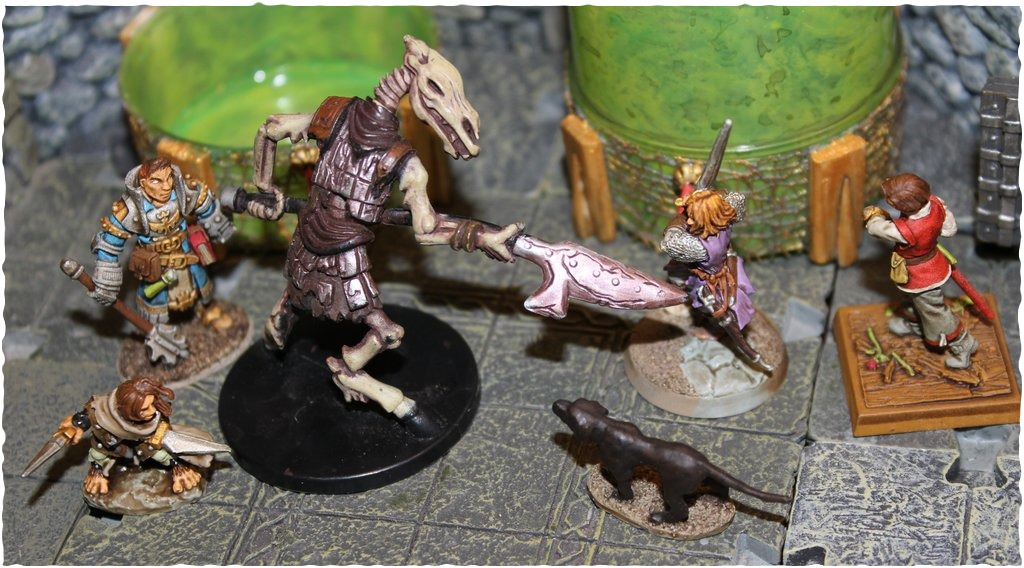
\includegraphics[width=0.4\textwidth]{images/Leukodaemon-523050841_mod.jpg}
	\caption{Leukodaemon}
	\label{fig:Leukodaemon-523050841}
\end{figure}



	%!TEX root = ../crimson_throne_book_main.tex
% 2015-03-28
A set of double doors in the far wall is the only way to continue. Balian pushes open the passage to\hyperref[fig:Temple-of-Urgathoa-Inner-Sanctum-523051443 ]{ the inner sanctum, the heart of the temple's corruption } : a high-domed chamber with six basins lining the walls, containing foul bubbling liquids in distinct blue, green, red, purple, white and brown colors. Each fills the air with its own sharp reek, creating a noxious, eye-watering bouquet. At the room's center, rising from a wide pool of crystalline water, stands a golden statue, depicting a beautiful woman with a lower body of bones. She holds a scythe in her left hand. From the far side of the pool the high priestess of Urgathoa, the haughty Lady Andaisin, greets her visitors: "And so you have finally found your way to the heart of \hyperref[fig:Temple-of-Urgathoa-523050074]{ my temple } , you ignorant fools. Know that you stand in the mighty presence of the architect of your city's demise. You call this a terrible plague, while I know it as the gentle kiss of the Pallid Princess. Yet I am still prepared to show you mercy. Choose one of these colored scourges to become one with the goddess. Those who drink I shall only cripple, leaving you to enjoy the wonder of Urgathoa's gift as it quickens inside your flesh. Those who abstain are fools, not fit to house a divine offering. You may fall at my feet and I shall make your end swift!" \\

\begin{figure}[h]
	\centering
	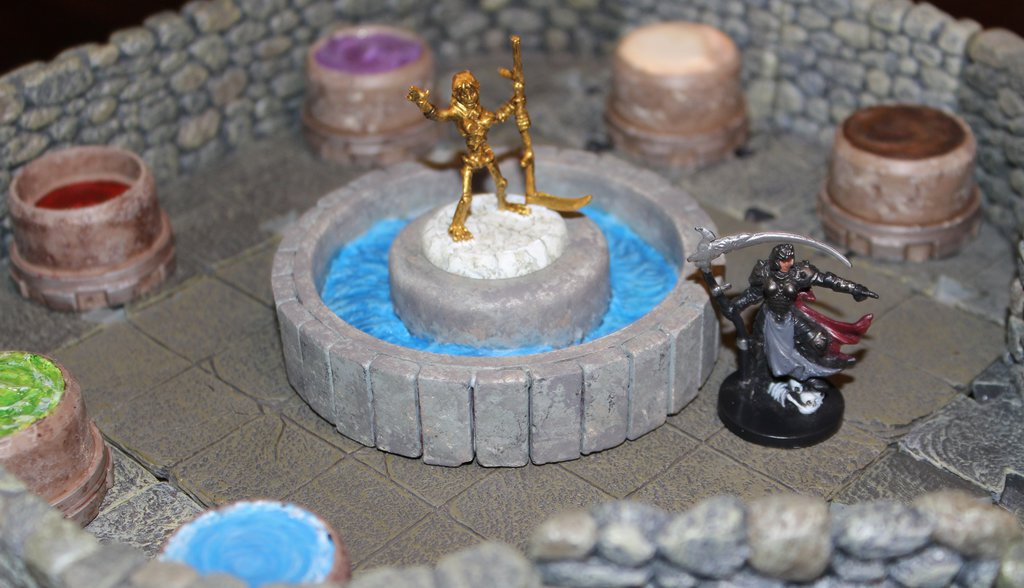
\includegraphics[width=0.39\textwidth]{images/Temple-of-Urgathoa-Inner-Sanctum-523051443 .jpg}
	\caption{Temple of Urgathoa Inner Sanctum}
	\label{fig:Temple-of-Urgathoa-Inner-Sanctum-523051443 }
\end{figure}

\begin{figure}[h]
	\centering
	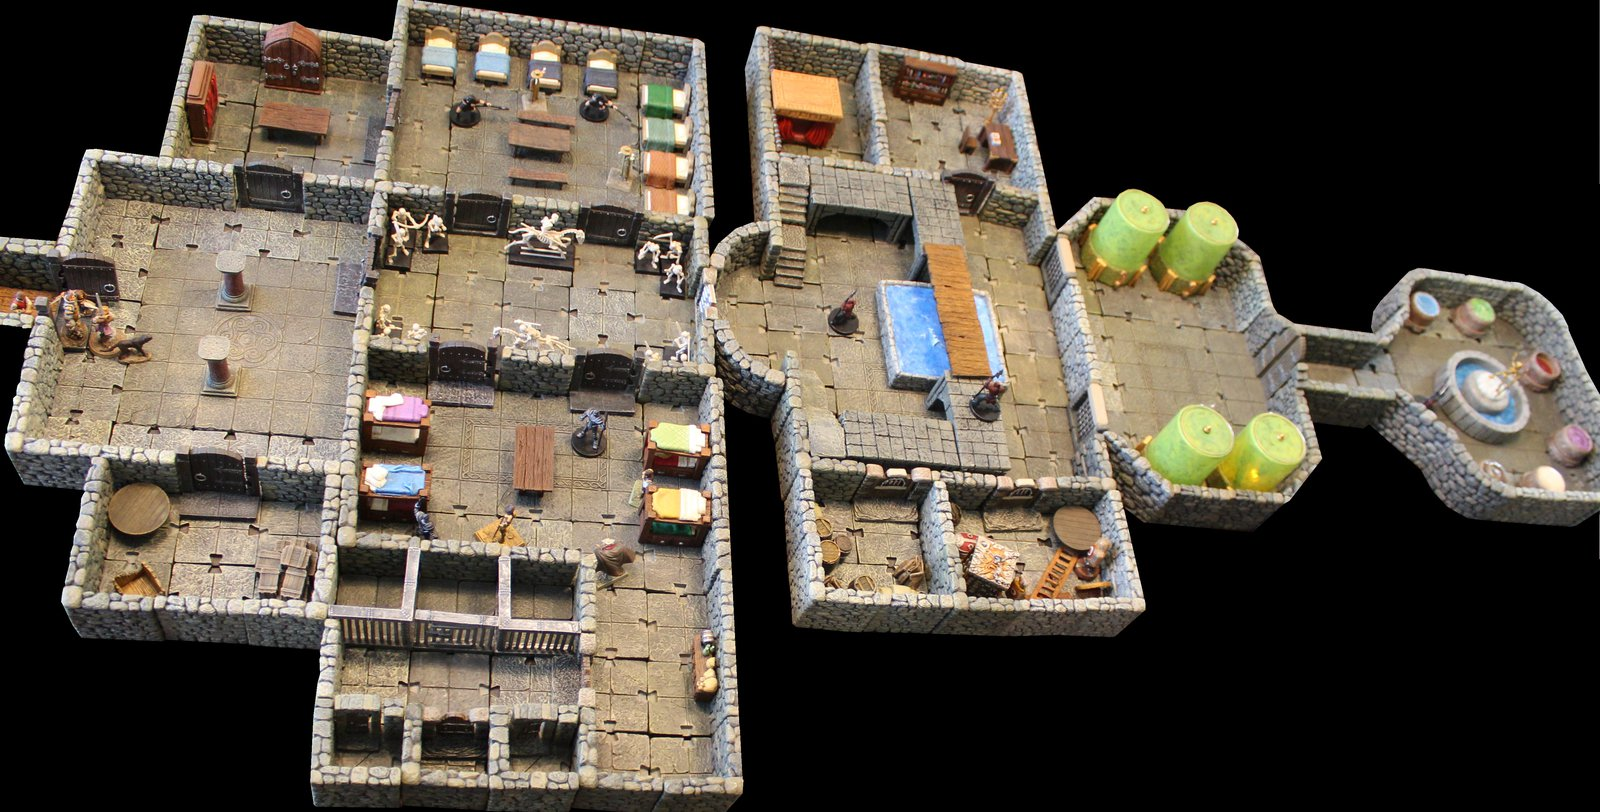
\includegraphics[width=0.39\textwidth]{images/Temple-of-Urgathoa-523050074.jpg}
	\caption{Temple of Urgathoa}
	\label{fig:Temple-of-Urgathoa-523050074}
\end{figure}

Puk is the first to react and rushes into the room, making his way around the pool. He leaves his friends at the entrance, who suddenly see the golden statue come to life and jump down from its stone pedestal in the middle of the pool, landing between them.\hyperref[fig:Statue-of-Urgathoa-attacks-523052019]{ The animated sculpture swings its scythe at Balian } and as she connects with his flesh, the brown pool starts boiling, claiming some of the ranger's strength. Next Lady Andaisin simply steps into the air, as if walking on an invisible set of stairs. Sjo realizes that she is under the effect of an  {\itshape air walk} spell, which will make fighting her very tricky. As he prepares an attempt to counter her flight magic, the priestess calls down a vengeful pillar of fire from her goddess, catching Quint, Sjo, Balian and Spyder in her  {\itshape flame strike} . The Shoanti healer laughs as most of the fire glides off his skin and throws his  {\itshape dispel magic} at the woman, sending her back down to the floor. The companions focus their attacks on the statue first, managing a few deep cuts in her golden skin. Her sharp scythe cleaves through the air with heavy swoops, missing only by a hair's breadth. Puk replies with two biting sneak attacks. Quint trips the thing with his whip, giving Balian the opportunity to finish it off. Meanwhile Sjo tries to keep Lady Andaisin busy. She easily resists his  {\itshape hold person} and prays for another  {\itshape flame strike} on her enemies' heads. Fortunately Balian is the only one who suffers the full effect of the unholy fire. \hyperref[fig:Facing-Lady-Andaisin-523052184]{ The fight now moves to the other side of the pool } , where Lady Andaisin is starting to lose the cocky grin on her face. She takes some heavy damage and, even though she succeeds at taking Puk out of the fight with a  {\itshape blindness} spell, she is sorely pressed. She looks quite proficient with her scythe, but being outnumbered four to one, she does not stand a chance. When she carves into Balian, Spyder reacts furiously and takes her down with his ferocious bite. \\

\begin{figure}[h]
	\centering
	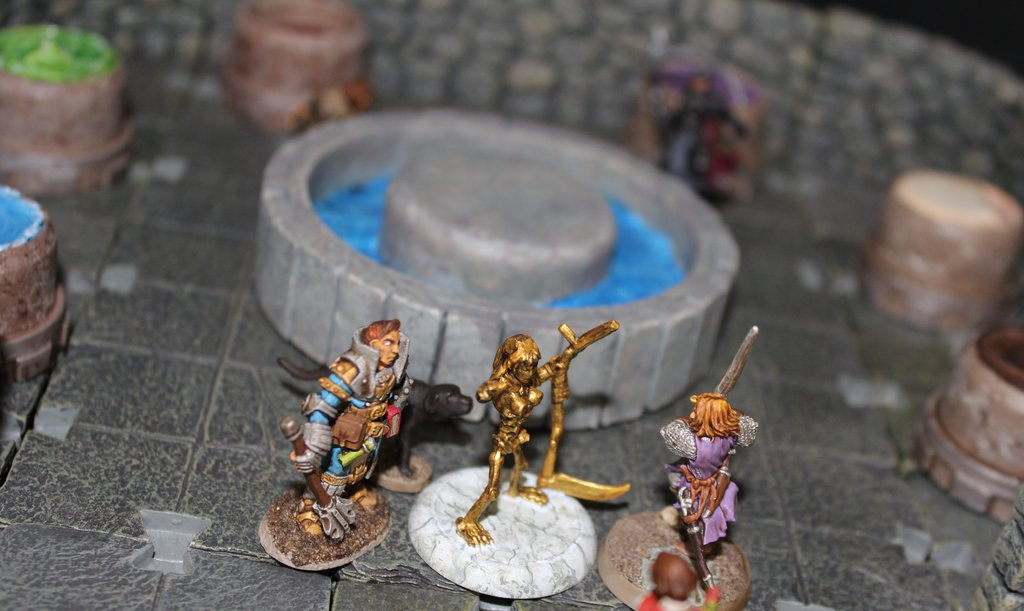
\includegraphics[width=0.39\textwidth]{images/Statue-of-Urgathoa-attacks-523052019.jpg}
	\caption{Statue of Urgathoa attacks}
	\label{fig:Statue-of-Urgathoa-attacks-523052019}
\end{figure}

\begin{figure}[h]
	\centering
	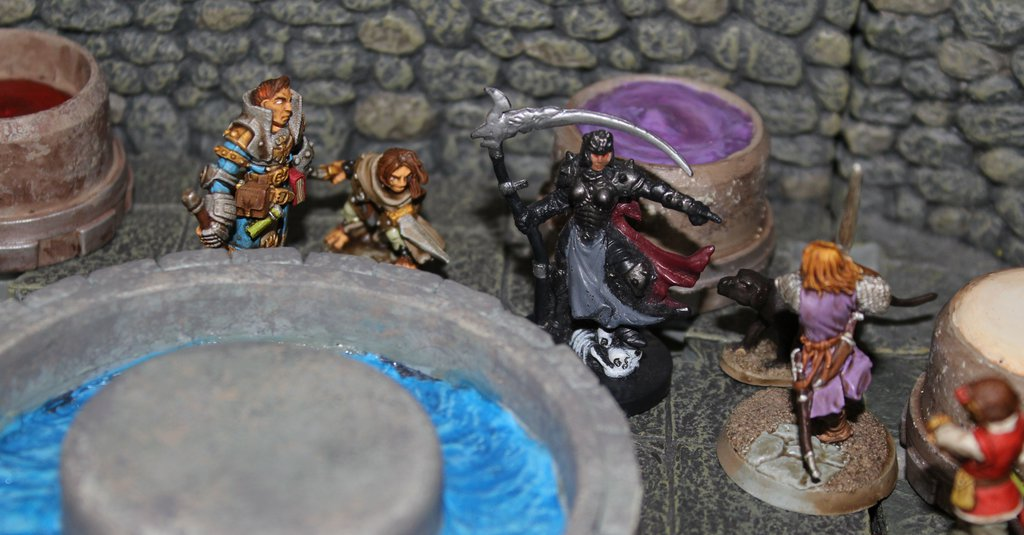
\includegraphics[width=0.39\textwidth]{images/Facing-Lady-Andaisin-523052184.jpg}
	\caption{Facing Lady Andaisin}
	\label{fig:Facing-Lady-Andaisin-523052184}
\end{figure}

A feeling of peace immediately descends upon the room. The colored fluids stop bubbling and the golden statue melts away in vile slime. So much for a well-deserved reward in pure gold, although it looks like Andaisin is wearing some valuable magical items as well. So there still is some nice loot to be divided, albeit that such treasure always comes at a price, literally: ten percent to the city's coffers. Quint gets sick just thinking about it. Still, he feels no qualms when he claims Andaisin's strength and constitution boosting girdle and hands her {\itshape headband of inspired wisdom} to Balian. Sjo is happy to take two powerful wands off Andaisin's dead body: a  {\itshape wand of remove disease} and one of  {\itshape cure serious wounds} . 

	%!TEX root = ../crimson_throne_book_main.tex
% 2015-03-28
 

	%!TEX root = ../crimson_throne_book_main.tex
% 2015-03-29
 

	%!TEX root = ../crimson_throne_book_main.tex
% 2015-04-03
The companions tie up Lady Andaisin and leave her in the room leading up to the sanctuary, with the green alchemic vats and the dead leukodaemon. Then they return to the cell block - where Rolth, Saulus and Alika are still locked up - letting the boy and girl they rescued earlier know that the priestess and her minions down here are all dead. They drag Rolth's unconscious body to the hall with the huge basin and the catwalks and use a {\itshape cure light wounds} to wake him up. It takes the necromancer a while to realize who About two and a half months ago Doctor Saulus sought him out in his secret den in the graveyard, Rolth confesses. He adds that he no longer uses this hideout as it was discovered during his time away from the city. He is not surprised to learn that the companions were the ones who shut the place down and killed his derro friends. Doctor Saulus - or Devils as he preferred to be called - promised Rolth to help him build his flesh golem if the necromancer took him in and allowed him to use his laboratory. Seeing an opportunity to achieve his life-long ambition, Rolth quickly agreed. When Sjo and Balian tell him that the golem was not nearly as powerful as Rolth believed, since they destroyed it very easily, a twitch of disappointment sweeps over his blotchy face.\\

Quint and Balian have trouble hiding their absolute disgust for their prisoner and tell him that his interrogation will determine whether he gets a quick or a long and painful death. They already butchered all the physicians and cultists in here, and they won't hesitate to give him what he deserves either. Rolth nods and chuckles: {\itshape``You may free Korvosa of the old Rolth, but it looks like there are four new Rolths ready to take his place, just as ruthless and deadly. I guess the city will be even worse off with the four of you \ldots}'' Sjo grabs the necromancer by the head and pushes him in the foul water of the room's central pool. Of course, this kind of torture only proves Rolth's point, who no longer feels inclined to answer the companions' questions if they will just kill him afterwards. Quint argues that the judicial system in Korvosa would only come to the same conclusion and condemn him to be hanged, seeing how he's been wanted by the law for many years. Hanging judge Zenobia Zenderholme is famous for her harsh judgments, so someone with Rolth's record would be judged very quickly.\\

{\itshape``Well, if you're so sure that the judge will hang me, you won't mind handing me over to the law. I'll make you a deal, I'll tell you everything I know if you can guarantee that I will get a fair trial. As you say, I'll die anyway, so it hardly matters to you. Give me your word and I'll tell you, but if you want to kill me here and now, you might as well do it now, for then I won't tell you anything.}'' Quint leaves it up to Balian to decide, being Alika's brother he harbors the deepest grudge. The ranger agrees, but the deal will be off if Rolth tells even the slightest lie, he says.\\

After this promise Rolth continues his confession. He bought the young female lambs from Gaedran Lamm for himself, but gave them to Doctor Saulus when he needed test subjects for his experiments. He took Alika so many years ago and he somehow liked her enough to keep her alive. He did play mind games with her, constantly telling her that her brother Balian had abandoned her and that he was a coward and a traitor. He repeated this over and over until she ended up believing him and voluntarily chose to join him.\\

As far as Saulus is concerned, the doctor looked Rolth up in the month of Gozran because he needed a place to brew a poison. Rolth did not know Saulus before that, but was willing to help out a fellow follower of Urgathoa. Although the doctor never told him what the poison was for, Rolth figured it was for the king. He does not know who Saulus was working for or who collected the poison, though. Then Saulus got a new assignment and asked Rolth to join him in Lost End, where they were joined by Lady Andaisin and her followers. These new allies all came from Cheliax and must have used teleportation magic to get there, though Rolth claims having no knowledge of who transported them. This was where the high priestess of Urgathoa enchanted the avian masks and she and Saulus developed the plague by experimenting on a number of people, including Rolth's girls. The necromancer himself spent most of his days constructing his flesh golem. They finally returned to Korvosa aboard the Delivery, but they abandoned ship and landed their sloops on the shores south of the city, where they set up camp. Rolth sneaked back in to the city, only to discover that his hideout had been compromised and his derro associates killed. He rejoined the Urgathoans and came to the Hospice after they acquired the place. He also claims that the Urgathoans entered the city undercover and somehow got into the castle, where they were supposedly 'teleported' to. This suggests that at least someone in Castle Korvosa was in on the conspiracy.\\

The companions tie up Rolth again and put him back in his cell. First they want to examine the three doors in the hall they used to interrogate Rolth, since they skipped those earlier. Two doors lead to storerooms, one with all kinds of trash and one with supplies. The other door opens into Andaisin's office. Balian finds a chest with a top-notch alchemy set, while Quint and Sjo examine the many books and notes. Puk, who is still blind, has to limit himself to listening if no one else approaches. There seems to be a large collection of volumes from the {\itshape Andoran Alchemical Society} , as well as extended notes on the experiments that Andaisin and Saulus carried out. The scribblings are quite complicated, though, and would definitely require a trained mind to be correctly interpreted. Professor Sirtane Leroung could certainly use these in her quest for a cure. A secret door leads to a bedroom with a very luxurious bed. There is a traveling chest with woman's clothes and a small box which holds some jewelry. Next on the companions' interrogation list is doctor Saulus. They head back to the cell block to get the bastard, but they are stupefied to find out that Alika and Rolth are missing, and Saulus is dead, his throat cut! Stable boy Dalvun and Jaelle, who are both resting in the bedroom that leads to the prison, have seen or heard nothing or no one. Alika's bonds lie on the floor of her cell, as if she slipped out of them. Damn those rogues and their slippery tricks! Balian also discovers two small iron needles, part of a thieves' toolkit, which Alika used to open the locks. Quint finds a lingering aura of {\itshape conjuration} magic in Rolth's prison cell, probably pointing at some kind of teleportation magic. The companions are very disappointed and swear never to make this mistake again. Fortunately, Lady Andaisin is still in their hands, as they kept her in another room. They drag her back into the inner sanctuary, determined to test out what effect the colored basins will have on her. Lady Andaisin, only smiles when threatened with submersion in these waters: {\itshape``Urgathoa is at my side! I've done her proud with my work in this city, so I'll be in her best graces when I cross over to the other side.}'' Sjo grabs the woman by the hair and pushes her face below the waterline of the blue liquid. In the process he gets his own hands wet as well and feels the liquid draining him. In reaction he drops the priestess to the floor, where she starts mocking him. Quint realizes that he and his friends are starting to behave irrationally, as Rolth's words still ring in his ears: {\itshape``four new Rolths ready to take my place}''. Andaisin remains confident that she will be rewarded in the next life, and one of the many pleasures she will be awarded with, will be the power to create undead. She will make sure that the companions' earthly remains will be used in such perversions. Quint gets quite angry with her while she claims she does not know who hired the Red Mantis. And even if she did, she would never tell them. Sjo also tires of her haughty behavior, she has nothing left to tell them, so he just bashes her skull.\\

As morning is fast approaching, the companions head back up to the hospice. They lure the last remaining doctors into the backroom and dispose of them. Next they collect the books and the survivors downstairs and simply walk out of the building, telling the remaining guards and Gray Maidens to check downstairs, leaving them behind dumbstruck. First they head to the university to give the books and notes they found to professor Sirtane Leroung, who is very happy to get this vital information. Next they want to inform the Field Marshal, but for the first time since they've met her, they do not find her at the Citadel, but rather at home. After waking her from her bed, they bring her up to date. Quint gets quite angry with her for allowing her Guard to be used for evil. Aiding the enemy is a grave mistake and in this case, assisting the physicians resulted in many deaths.\\



	%!TEX root = ../crimson_throne_book_main.tex
% 2015-04-18
The sun is already rising over the horizon when the companions finally get home. The kids greet them enthusiastically and want to know everything that happened, but Sjo just tells them that he and his friends have completed their mission successfully and want to go to bed. The Shoanti quietly sneaks into his bedroom, where Madam Nesia is sleeping in the other bed. He noticed that her breathing is heavy and she's coughing. The tall healer puts his hand on her forehead and feels that she has a temperature. He pulls out his {\itshape wand of remove disease} and heals the ailing woman without waking her up. When her breathing eases, the weary warrior quickly slips between his own sheets for a couple of hours of overdue rest. Our young friends get up in the afternoon, slightly surprised that no one came to get them out of their beds to ask them about their deeds last night. Madam Nesia is still sick, despite the fact that Sjo was sure he cured her last night. Her eyes are red and she is feverish. Sjo examines her and comes to the conclusion that she is not suffering from the plague. He wonders if she might be cursed and shares his concerns with the others.\\

After a hearty meal the companions head over to the temple of Sarenrae to get Puk's blindness removed. There they learn that the patients of {\itshape the hospice of the Blessed Maiden} are all being moved to the hospital of the medic temple task force, after the Queen's physicians have been exposed as traitors who were spreading the plague in the name of Urgathoa. Fortunately the  {\itshape Gray Maidens} discovered this deception and took care of the problem, permanently! Quint is shocked by these rumors: so now the Gray Maidens, who were foolish enough to let themselves be tricked by the doctors, think they can steal the glory of solving the problem?!? And no one even thought it necessary to consult the true heroes about this fabricated story?!? Quint is quite upset and wants to confront the Gray Maidens, but Sjo convinces him to go to Kroft first. After all, Puk figures, if the companions want to keep a low profile, this story is the perfect cover. It wouldn't be smart to shout all over town that they are the ones who really cleared the Urgathoan temple of its cultists. Those Red Mantis assassins might still be out there and it wouldn't be wise to call too much attention to themselves, the rogue explains. Field Marshal Kroft already knows the truth, so talking to her might be smarter. Perhaps she can shed some light on the Maidens' motive behind this lie. In the Citadel Quint first apologizes for his outburst this morning, when he accused the Field Marshal of - unknowingly - aiding the enemy. Kroft is happy that he is not angry at her anymore, but says that he was right: she feels bad about the Guard's involvement in the physicians' foul plans. When the bard asks her about the reasons why the Gray Maidens want to claim the honor of clearing the temple of Urgathoa, Kroft replies that she was not consulted in that decision either - she is never consulted anymore; she is just told what to do. If she has to guess, she would say that the Maidens feel ashamed as well for assisting the cultists in spreading the plague, so maybe they want to make up for their mistake in the eye of the public by claiming to be the saviors who solved the problem. Kroft and her guards who were present at the Hospice this morning, have been ordered to keep quiet about the true heroes' involvment.\\

Quint starts wondering who is behind all these evil schemes. The list of possible suspects is just too long. Is Ileosa herself evil? If she wanted the throne for herself, she could be responsible for having Eodred killed, but why would she kill off half her subjects by ordering a plague to be brought down on Korvosa? Sjo utters the possibility that she is an Urgathoa fanatic herself. Or is Sabina Merrin corrupted? As commander of the Gray Maidens she has certainly moved her own troops into a position of power. Maybe one of the noble families is involved: they killed the king, hoping his queen would prove incompetent and one of them might step up to take the empty throne. Or are the banished Porphyria's engineering a return to Korvosa and its highest seat?\\

According to Kroft Ileosa also has a new advisor, a wizard from the Acadamae. Is he the puppeteer who controls the queen and her entourage, possibly working in the service of the Ornelos family? And what is Selena's role in all of this? The manipulator has always claimed that the queen is evil and that she is working for someone who wants to save Korvosa. There are so many options. One thing is sure, someone in the castle has been compromised. They worked with the doctors, allowing them inside the castle and then making up some story that the physicians were teleported in from Cheliax. Still this knowledge makes reporting to the castle a risky venture. How can you figure out what goes on in the castle without being in the eye of the traitor? Field marshal Kroft says that this has always been the task of the seneschal, but with Kalepopolis gone, there is no one to keep an eye on things. She could possibly get an audience with the queen herself if she insisted, but what would be her goal? She could never find out anything about the traitor without raising suspicion. Maybe commander Endrin of the Sable Company could be of more help, since the seneschal always comes from his ranks. Moreover, the Company is not tied down by the Gray Maidens as the Korvosan Guard is and Commander Endrin has been known to question the castle's recent politics before.\\

The companions decide to pay the commander a visit. Sjo is still welcomed in the Great Tower with open arms and immediately gets an audience with Marcus Endrin. The commander is pleased to see the Shoanti and thanks him for saving his stable boy Dalvun last night, but he is also baffled by the Gray Maidens' claim that they cleared the Urgathoan temple. Still, just like the young heroes, he cannot tell whether this Gray Maiden lie is inspired by treachery or a feeble attempt to mask their own incompetence. Sjo comes clean and informs the commander of everything he and his friends found out over the last couple of months. He also presents the commander with the evidence they uncovered: the Red Mantis letters to Doctor Devils, ordering him to first concoct a poison for the king and then to bring down the plague on Korvosa. Endrin is definitely on the same page as his visitors. He has no love for the queen, fearing that she is the evil behind all of Korvosa's recent trouble, and even if she is not, she allows herself to be manipulated, which also makes her incompetent to rule. If only the seneschal were here to take control: he could remove the monarch from power to regain control of the city and weed out the evil at its heart. Endrin has pleaded for a new seneschal before, but his request has been countered with the uncertainty of the last seneschal's fate. Is Kalepopolis really dead or is he still alive, and if so, where is he? Quint and Sjo wonder if his fate could be determined magically? The commander encourages them to enlist the help of one of the temples and try to find out. He will also resume his efforts to see the seneschal replaced with a new Sable Company man. First he will appeal to the queen herself to install a new seneschal and if she refuses, the council of nobles could enforce it. Quint fears that a new seneschal might quickly be manipulated himself by the evil force in the castle, but the commander argues that this new seneschal could act immediately. He feels that there is enough evidence to remove the monarch from power, permanently of temporarily, to regain control of the situation. Quint doubts that this law-abiding approach will succeed, but cannot offer a better alternative. He and his friends will continue their efforts to find out more while the commander exhausts all legal ways to see order restored. The two parties agree to keep each other informed of their progress.\\



	%!TEX root = ../crimson_throne_book_main.tex
% 2015-04-25
Upon returning to the villa, the companions find that Madam Nesia's condition has grown worse. She is delirious, suffering from high fever and hardly aware of her surroundings. Our friends decide to summon Zellara's ghost from the Harrow deck to consult her. Maybe she can find out if the girl is cursed. The ethereal gypsy bends over the sick woman and holds her hands over her head and body, sinking into an intense trance. Her face betrays the effort it costs her and Balian is sure he sees drops of sweat dripping down her ghostly face. After what seems like an eternity Zellara gets up again, obviously exhausted. She states that she has trouble finding the poor girl's soul.\\

"Does that imply that she has no soul?" Quint wonders.\\

"There is something there," Zellara replies, "but it keeps slipping out of my reach."\\

Having heard stories of people who sell their souls to devils, Sjo immediately suspects the church of Asmodeus to be involved. Balian suggests to take the girl there and have the priests of the {\itshape Prince of Hell} look at her. It might be risky, but it seems like the most direct route to an answer. The others agree and prepare the carriage to transport Nesia across town. However, when they try to lift her from the sofa, her arm bruises badly from the slightest touch. Using the sheet on which she lying instead to carry her, the party gets her to the coach and takes her to the steps of the Archfiend's house. Sjo knocks on the door and is met by Mallas, the highpriest's grim personal bodyguard. The stern warrior does not feel inclined to help the Shoanti who once came to the temple as an aspiring acolyte and then betrayed this 'contract' by turning his back on the Lord of Oaths. It takes some convincing until he finally agrees to let them in. The heroes gently place Nesia on the altar, which is conveniently shaped to support a person's body, and wait for highpriest Reebs to arrive. Reebs does not understand why the party brings him a sick girl, he is not the city's prime authority on healing and his contract with the medic task force - which the companions helped negotiate - has already cost him all of his healing magic for the day. Sjo explains that they are not here for his medical expertise, but rather for his extensive knowledge on the nature of souls.\\

When Ornher Reebs turns towards the girl Sjo detects a hint of surprise on his face, which the man quickly hides. He gives her a fairly shallow look-over while Quint explains how they found the girl in the street, devoid of any memory. Reebs looks at the companions and chuckles. "She's naught but an empty shell", he claims. "Just take a dagger and prick her with it".\\

Puk draws his blade and carefully sticks the point in Nesia's upper arm, where the bruises are. Blood pours profusely from the tiny wound, while the girl starts shaking badly. Her body jerks upward in a sudden, spastic motion and completely turns into blood. The fluid spatters the bystanders and falls down on the altar and floor, leaving no trace of any person: no body, no bones, no skin, nothing but blood. The companions are flabbergasted and even Ornher Reebs regards the spectacle with a shocked look in his eyes.\\

"Well, that is a new experience, all right," the highpriest utters, breaking the silence. It is obvious that he's never seen anything like this either. Quint's mind races to find an answer: Was Nesia ever human? Maybe she was some kind of simulacrum, a copy of someone else, although those are normally made of snow and ice, not blood. Reebs claims not to be familiar with the concept of blood clones, but supposes that it could be possible. Of course, this might mean that the original version of Nesia is still around somewhere. Puk takes a bit of the blood for later examination and the companions leave after making a contribution to the temple's coffers of 50 gold pieces - which Mallas finds insultingly low.\\

Before turning in for the night, the young heroes get the sole surviving plague doctor from the old fishery and hand him over into the custody of the Sable Company.\\



	%!TEX root = ../crimson_throne_book_main.tex
% 2015-04-25
\section{8 Erastus 4708}

The next morning Sjo pays his girlfriend Larella a visit in the medic force hospital ,which is overflowing with the extra patients who were brought over from the Hospice of the Blessed Maiden. He helps out for a while, taking care of the many sick.\\

Quint has set his mind on infiltrating the castle as a servant and decides to stake out the place for a couple of days to get a picture of the every-day comings and goings at the palace. He dresses up as a commoner and hangs around Castle Korvosa for the rest of the day.\\

Meanwhile his friends head over to the temple of Pharasma to sell off some of the loot they found. Brother Cedrik, the priest they saved from the undead in the catacombs under the mortuary, is the acting accountant they have to deal with. Sjo asks him if anyone in the temple would be able to find out if a certain person has already passed through Pharasma's Boneyard or not. Cedric is no expert on the matter, but says that the Lady of Graves is not known for sharing such knowledge with mortals. Strange as it may seem, divination is much more the domain of wizards than priests, especially if you have specialists on the subject. The Acadamae definitely has an accomplished diviner, as every school of magic is taught there by an experienced professor. Of course, the Acadamae has never had an open-door policy and since the death of the king they have secluded themselves even more from Korvosan society than before. So getting in touch with this person might prove very challenging. Sjo uses some of the new funds to pay off last month's tax debts and buys two magical bucklers for Quint and himself. He also gets a {\itshape potion of remove blindness} for the next time Puk gets robbed of his sight. Better safe than sorry, he figures. At the university of Korvosa, alchemist Sirtane Leroung is still working on a cure for the plague. She is very hopeful: the books and notes which the party brought her from the temple of Urgathoa, prove a big help in her research, even though they do not mention a remedy as such. She is also performing tests with the immune Varisians' blood. Puk pulls out the vial he filled with Nesia's blood last night and asks professor Leroung to take a look at that too when she has the time. He does not tell her where it comes from, though. Sirtane says that her priorities lie with the cure for now, so it may take a while before she can spare a moment, but when she does, she will be glad to examine the blood. She also refers the companions to Tepest Geezlebottle, the gnome professor and headmaster of Theumanexus College, Korvosa's smaller school of wizardry, for advice on divinations.\\

Puk, Sjo and Balian make a quick stop at the Citadel and ask Field Marshal Kroft to have a wanted poster made for Rolth. They agree to put up the reward money of 1,000 GP if the necromancer is brought in alive. Afterwards they head to Geezlebottle's school. The gnome wizard is no master of divination, explaining that the most efficient spell to get an answer to the question if someone is still alive, is {\itshape contact other plane} , but such powerful magic comes at a high risk: the wielder of this magic runs a substantial chance of losing his mind for a couple of weeks, the worst fate a magician can suffer. Moreover, Geezlebottle does not know this spell, as far as he knows, only Norva Allesain, the head of the divination ward in the Acadamae, does. The gnome does master the art of  {\itshape scrying} , which might indirectly prove that someone is still alive. He agrees to study two of these spells for tomorrow. 

	%!TEX root = ../crimson_throne_book_main.tex
% 2015-04-30
Meanwhile at the Castle, Quint has been watching the grand stairs leading up the pyramid. Four Gray Maidens stand guard at its foot. By half past nine the doors of a nearby building, just left of the stairs, open and a strapping young man, about Quint's age, leads out a horse and cart. He seems familiar with the animal and talks to it soothingly while staring up the stairs to a small group of people coming down. A middle-aged woman and a young girl, who looks no older than fifteen, are accompanied by four Maidens. The girl waves vigorously at the young man and allows herself to be helped on the box. She fakes having trouble getting up, so the man has to lift her. She clearly enjoys the attention. The driver also aids the other woman take a seat before he sits down himself and gently urges the horse to move. The four Gray Maiden fall in line behind the wagon and follow it to the east.\\

Quint pursues the wagon from a safe distance to the market. The middle-aged lady buys all kinds of supplies, enough to feed at least  two dozen people easily. The merchants greet her kindly and allow her to cut in line. The goods she requires are already waiting for her and while she pays and specifies what she'll be needing tomorrow, the merchants' helpers load the merchandise in the wagon. The whole process runs very smoothly and Quint sees no opportunity to interfere without raising suspicion. He does learn the woman's name, as the merchants address her as {\itshape Mrs. Karina} . The young girl remains at her side at all times and while they're buying meat, the butcher hands her an extra piece of sausage and calls her  {\itshape Mikki} . The man is obviously charmed by the lass and again she seems to welcome the attention with a warm smile. Quint then decides to try and approach the driver while he's waiting, but the Gray Maidens step up immediately and urge him to move along. Perhaps he'll have better luck at the stables, where at least there are no annoying Maidens around.\\

When the shopping is done, the wagon returns to the castle, where a broad-shouldered, but simple-looking man is already waiting for it to arrive. He picks up a heavy basket and joins the four guards and the two women up the stairs to the castle. The man comes back two times more to carry up the rest. Next the driver takes the wagon back to the stables.\\

In the streets at the foot of the pyramid Quint addresses a woman who also looks like she's just returning from the market. She puts her basket on the ground and reaches for her keys to open the door.\\

"I"m sorry, ma'am, I just noticed a sweet little dog around the corner. It looked well cared for ... white, with a long fur and a face like a fox. It can't have been a stray, but its owner was not around. Maybe it slipped out of the house or something. You wouldn't happen to know who owns such a pet?"\\

"A white dog, you say? Sorry, I can't help you there. No one around here owns such an animal." The woman pushes her door open and reaches for her basket.\\

"Are you okay with the groceries, ma'am? Too bad you don't have a strong man to help you carry your things, like that fellow I just saw on the steps of the castle. He seemed like a friendly chap, though not too bright."\\

"Well, we can't all be queens, can we? That Jorn fellow is indeed somewhat of a simpleton, but he's a good boy. He's been working there for as long as I can remember.\\

"Like part of the furniture?" Quint laughs. "Do you know if they're hiring people up there? I'm actually from Old Korvosa, but ever since the quarantine I've been locked out. I can't go home and I can't do my job. It doesn't look like I'll be able to get back any time soon, so I'll have to find something to earn a living in the meantime."\\

"Oh no, poor boy, here ... have some of my bread."\\

Quint refuses to take the loaf: "That's not what I mean ma'am. I have a few coppers left, I don't need a pittance. My mum didn't raise me to be a beggar. I want to work for my money and make an honest living. Such a big castle always needs people, doesn't it?"\\

"Well, it's mainly women, up there. This Jorn fellow is an exception because he's been there for so long. The men work down here, in the stable with Master Jacob."\\

"Aha, I might give him a try, then. Thanks for the tip, ma'am. I wish you a wonderful day."\\

"That very kind of you, young man. I wish you the same." At that the woman goes inside.\\

Quint keeps an eye on the castle for the rest of the day. At two o'clock two dozen Gray Maidens arrive from the east and go up the stairs. Fifteen minutes later the same number of female warriors comes down again. Four of them relieve the sentries at the foot of the stairs, while the others leave again. Quint follows them over the High Bridge into the East Shore district, at the other side of the river. They enter a walled complex just across the water. So these are the Maidens' barracks, good to know.\\

---\\

Sjo is still working on finding out whether seneschal Kalepopolis is still alive. He decides to check with archbishop Keppira d'Bear herself at the temple of Pharasma to find out if she can help him. She confirms his suspicion that high level priests have an excellent spell for just such a purpose: {\itshape commune} . With this magic she can contact her deity and ask a number of questions that can be answered with a simple yes or no. She is not surprised that brother Cedrik did not know about this spell; he was always better at keeping the books than at weaving magic, as his tragic mishap under the mortuary clearly illustrated. Keppira d'Bear is also the only priest in her church who masters this level of complexity. While she dislikes the fact that she would have to give up a spell that might cure another plague victim, she does agree that Pharasma is the prime authority on life and death. If Sjo can offer some relief for her cure-wasting guilt, she'd be willing to pray for a  {\itshape commune} spell tomorrow. She also explains that he has to prepare his questions carefully. The magic allows her only a short time to ask about a dozen things, wasting these precious seconds to come up with new questions is not an option. Sjo freely offers one of his  {\itshape wands of remove disease} - the one with 11 charges left - to d'Bear as compensation, which she gladly accepts. ---\\

Puk decides to dive into the villa's library. He is quite ambitious, putting one book on top of the other, he wants to make a pile as high as he is and read that! Still, looking at all those books, he realizes that he'd better start with some light reading and takes a small book on halflings in Korvosa. Perfect! Now he can find out which other famous kinsmen were here before him. It turns out that the history of famous halflings still has to be written. The book details how the Leroung family uses ships with halfling crews, who are lighter and take up less space than human sailors, so the ships can carry more goods and turn in a bigger profit. So the chronicles of the smallfolk in the city limit themselves to servants and workers. Even the most 'famous' halfling in Korvosa was once a servant. Old Orkatto, the owner of {\itshape Orkatto's Feathers and Furs} , used to serve a lord in Magnimar as his master of the hunt. The country squire saved his coppers well and retired to Korvosa to set up a shop in exotic pets. His caged wonders go from rainbow-plumed songbirds and snowdust badgers to emerald-back nightbelly boas and even the odd dream spider. Apparently, the shop is in South Shore, quite close to the villa. ---\\

Later that day Balian sneaks off on a private mission. He remembers the Sczarni thugs who attacked him and his friends when they were in Path's End for the first time. Back then his party was no match for these gangsters and needed Grau Soldado's help to escape, but the ranger's skill has grown considerably since that time and now he feels confident that he can handle a little trip to Thief Camp by himself. He does take Spyder along, just in case things come to blows and he needs a flanking partner. His goal is to find the Scarni's {\itshape godfather} , a man called Batista Cadabrani, and enlist his help in tracking down his sister Alika. Being a fellow Varisian, Balian hopes that these Sczarni will agree to sell him their services. After all, the Sczarni are notorious for standing up for Varisian rights and punishing the Chelaxians on their high horses. Located just outside the city walls beyond Dwarfwalk Gate is the shantytown {\itshape Thief Camp} . Balian notices that the poor people here have not been spared from the plague: there are crosses on several doors and a dozen dead rats and people lie by the road, ready to be carried off. Balian spots a few local thugs and approaches them without showing any hesitation: "I want to meet with Batista Cadabrani. Take me to him", he calmly speaks. The biggest gang member mocks the ranger: "And who is this little mouse in a rats' nest? It looks like you need an urgent lesson in humility!"\\

Balian sighs and holds his head at an angle. "I bet I can take you down without even taking my hands out of my pockets", he claims. The man fumes and reaches for his club, but Balian simply whistles for Spyder to jump at the brute. A few breaths later the man is squirming on the ground, bleeding from several bites, begging for mercy. Balian calls off his canine and repeats his request to see Cadabrani.\\

The ranger is guided into one of the bigger stone houses, where an older man is cutting onions at a table. He's wearing a black brimmed hat and his gaunt face sports a shade of gray stubble. Despite the sting of onion in the air his eyes show no sign of tears. "Do you like onion soup, Varisian?" he asks. "It stimulates the bowels. When you get my age, not everything runs as smoothly as you'd like anymore, just like my men in the street. They seem to be having a hard time as well keeping things in hand. Sit down and tell me why you're here."\\

Balian explains that his sister has disappeared and that she was last seen in the company of Rolth the necromancer. Batista concurs that this Rolth character is like an eel, slippery and repulsive at the same time. He is also extremely hard to track down. Finding someone who is with him will prove very hard. Such a service will be expensive. Batista wants 100 gold sails per day for sending his men out to look for her and an extra 1,000 gold if they locate her. The payment for the daily search has to be paid in advance. If the money stops, so does the search. Balian stipulates that Alika has to remain unharmed or consequences will be dire. He also demands a daily report. "Do not try to con me, old man, or you'll pay the price that so many have paid who tried to cross me. I'll return shortly with the money."\\

As Sjo controls the group's income, Balian has no personal money to speak of. Asking his Shoanti friend is not an option, since the righteous healer might not agree to hiring an underworld gang to do some shady work. Selling one of his magic items looks like the only alternative. Fortunately he has just the item: Lady Andaisin's {\itshape headband of inspired wisdom} . The temple of Pharasma would definitely be interested in such an item, but Balian doubts if they will be discreet about it, so he visits a merchant who will do anything to make a profit, including keeping quiet: Diederik Lodann. Lodann was the merchant-actor who played alongside the companions in  {\itshape The Passion of Saint Alika} , portraying the seer's father. Balian secures a neat 2,000 gold sails for the headband and negotiates a buy-back option within ten days for a 10 % increase. With two bags of 100 platinum pieces Balian returns to Batista to seal the deal. He pays the gangster his first 100 gold and expects a detailed report tomorrow of what his money has bought him. "Of course, my dear Balian, for a Varisian hero like you, we will certainly do our best", Batista smiles. Although it sounds like a compliment, Balian senses that the old man wanted him to know that he already figured out who he was in this short time span. Well, at least this proves that the man has resources to gather information, but Balian will have to watch his step around him.\\

---\\

Concluding that he has done enough reading for the day, Puk sets out again to check the quarantine situation of Old Korvosa. Since halflings in Korvosa are considered simple workers or servants, no one notices the small rogue, who also uses his skill to blend into the shadows to remain unseen. The Narrows of Saint Alika, as the channel of water between the mainland and Endrin Isle (the actual name of the island on which harbors the district of Old Korvosa) is called, is mostly obscured from view by sturdy city walls that line the northern coast of the mainland. The many gates in the wall, which used to lead to the 20 or so wooden bridges over the Narrows, have all been closed, and the bridges behind them burned. A score of Gray maidens man the walls.\\

The only 'breach' in the wall is where the stone bridge crosses the channel. The opening has been thoroughly barricaded and is also heavily guarded. Peeking over the blockade, Puk notices several skiffs in the water with even more Maidens, who are guarding both the Narrows and the mouth of the Jeggare river on the other side of the Isle. In all, the security of Endrin Island seems pretty tight. Puk counts at least five dozen Gray Maidens. The halfling also gets a glimpse of the district on the far end of the bridge. Old Korvosa looks desolate; several buildings have been vandalized or burned and no one dares to show himself so close to the deadly guards on the bridge. The most gruesome discovery is the fact that the protestors who were killed when the bridge was closed, are still on the ground Their cadavers have been left to rot. This sight makes the halfling sick to the stomach. He can only pray that his appetite returns by the time he gets back to the villa, since he left a note for the boys: "Days in Korvosa always get me hungry, mountain man scale!"\\

---\\

Quint spends the rest of the afternoon spying on the castle, where nothing happens until early in the evening. Three hippogryphs carrying Sable Company marines land on the castle's terrace. From his vantage point in the street Quint can't make out what they do. Half an hour later they fly off again.\\

When the sun starts sinking towards the horizon Quint decides to take his chances at the stables. He addresses two boys who are filling troughs with water. "I beg your pardon, friends," he says, "I'm looking for master Jacob." One of the lads runs off and quickly returns with strapping man, who looks about 45. "You wanted to see me, good sir?"\\

"Good evening, master Jacob. My name is Marcus. I live in Old-Korvosa, or at least I used to, before the quarantine." Quint produces a sad puppy look on his face. "I'm actually looking for a job on the mainland and some of the neighbors told me to talk to you. Could you use an extra pair of hands around the stables? Or somewhere else, I'm flexible and I'm a hard worker ... I don't ask for much ... just enough to get by, you know."\\

"Well, I am actually short a few hands at the moment. I lost three of my men to the plague and three more are in the hospital. I can't promise you it'll be forever, but for now I could definitely use the help. Why don't you come back tomorrow, at sunset? We'll give it a try ..."\\

"That would be great, sir ... or should I call you master?"\\

"Master Jacob is fine. I'll see you tomorrow, Marcus. Don't be late. I run a tight shift."\\

"I'll be there, sir ... erh, master Jacob. You can count on me." Quint makes an awkward bow and walks out. That went well. Satisfied he returns to the villa.\\



	%!TEX root = ../crimson_throne_book_main.tex
% 2015-04-30
With a couple of days off, the PCs are free to pursue some of their personal quests. We're playing this mostly ad lib, as I've found that my players want to use every moment that is available to them. In order not to waste too many sessions on this at the gaming table and also to allow me some extra time to come up with a coherent response and check all my resources, I've decided to play out part of this by mail. The following report is the result of these mails. 

	%!TEX root = ../crimson_throne_book_main.tex
% 2015-05-09
That should have been sun {\itshape rise} , of course, don't know how I messed that up. 

	%!TEX root = ../crimson_throne_book_main.tex
% 2015-05-09
\section{9 Erastus 4708}

Quint gets two rooms at an inn, one in his own name and the one next to it as Marcus. This place will serve as his place of operations during his undercover mission. This means he will have to miss out on the {\itshape commune} session, though. Puk, Sjo and Balian attend the morning service in the Cathedral of Pharasma. Afterwards they meet up with Archbishop d'Bear for the divination attempt. "As I told your friend Sjo yesterday, you have come to the right place to ask your questions. Pharasma shepherds our world's recently-departed souls to their final reward. All have to stand before her throne in the {\itshape Boneyard} , to be judged. She alone decides where each of us will spend eternity. As goddess of life and death, she already foresees what our ultimate fate will be, which is why she is also the mother of prophecy. Still, she accepts that we all have room to shape our own destiny, which is why she reserves her ultimate judgement until we finally stand in front of her. You have proven yourselves friends of the {\itshape Lady of Graves} , and as such you have deserved this favor of her. But since we are all free to shape our own lives, the  {\itshape Mother of Souls} frowns upon divine interference, so she will bestow the honor of her insight upon you only once. I hope you came prepared, for your window of opportunity will close fast. Be ready, my friends, for you will not face the high one again until your day of judgement." Keppira d'Bear raises her hands to the skies, takes a deep breath, closes her eyes and utters the holy words. All goes silent and it feels like the world around the companions disappears, leaving only the here and now. When the archbishop opens her eyes again, they are white and she speaks in a voice that is not her own.\\

"MORTALS, YOU HAVE COME TO ME FOR GUIDANCE. ASK AND I WILL ANSWER."\\

Sjo can't help but feel impressed and needs a little nudge from Puk to snap out of his wonderment: "Gulp ... my Lady, we are humbled in your presence ..."\\

"Ask the questions", Balian grumbles under his breath.\\

"Oh yes, my Lady, is Neolandus Kalepopolis, the seneschal of Korvosa, still alive?"\\

"YES."\\

"Is he being held prisoner?"\\

"YES."\\

"Are Kalepopolis and Blackjack the same person?"\\

"NO."\\

"Is queen Ileosa Arvanxi a follower of Urgathoa?"\\

"NO."\\

"Is the one who ordered the plague on Korvosa a member of an old Chelish noble house?"\\

"YES."\\

"Is queen Ileosa involved in the murder of her husband Eodred Arabasti?"\\

"YES."\\

"Are there members of the Red Mantis assassins present in Korvosa at the moment?"\\

"YES."\\

"Are there Red Mantis assassins in the Castle?"\\

'YES."\\

"Was the Red Mantis contacted by Ileosa or someone of her entourage?"\\

"YES."\\

"Was the initiative to contact the Red Mantis taken by Ileosa?"\\

"UNCLEAR."\\

"Is the queen being misled by one of her advisors?"\\

"YES."\\

"Are Rolth the necromancer and Balian's sister Alika still in Korvosa?"\\

"YES."\\

"Did the artists Lucian Lycan, Guy Nolin and Archibald Meerwater die because of a shift in the pantheon?"\\

"NO."\\

Keppira closes her eyes again, releases a deep sigh and lowers her head. When she looks up again, she is trembling. "I have not performed this ritual often," she breathes, "it is the most wonderful paradox you can imagine, to feel the wisdom of the goddess flow through your veins, but our simple mortal coils were not meant for such wonders, so it leaves me exhausted and wanting at the same time. So strange, like a drug addicted drug addiction. You must excuse me, I must rest. I hope you found what you were looking for."\\

---\\

Meanwhile Quint has made sure to arrive at master Jacob's at sunrise, disguised as Marcus from Old Korvosa. The head of the castle's stables puts him to work immediately, helping to muck out the horses' stalls alongside the two boys he saw here yesterday: Wade and Pip. Although Wade is the older of the two, it quickly becomes clear that Pip is the smarter one. The twelve-year old boy is very helpful and tells Quint what to do. "Cleaning up horse manure is not a difficult job, as long as you are willing to get your hands dirty", the boy teases. "Or you can just be smart about it and use a pitchfork", he laughs, while showing the newcomer how to swoop up the wet and dirty bedding while leaving the clean stuff on the floor. "All horses are different", he explains, "it gets easier once you get to know them. Just make sure to be thorough, or it'll be twice as hard to clean up tomorrow." Afterwards he also teaches Quint how to empty the wheelbarrow in a large cart. "You'll have to take that out of the city later, with Curtis", he says.\\

Quint really digs in and makes an excellent impression on the boy. In the meantime he learns who else works in the royal stables. Old Docus is an experienced horse trainer who hails from the breeders in Harse. His sight has diminished greatly with old age, but he knows his way around the stables blindly. He walks the animals in the yard with the aid of Billy and Bowen, twin brothers who are about Quint's age. They were hired four years ago by king Eodred himself after their father, who was a hippogriff rider in the Sable Company, lost his life in the line of duty. Quint also meets Ron again, the man who took the cook and the servant girl to the market yesterday. Ron is new at this job, since Greg, the old driver died of the plague.\\

When the stalls have been cleaned, Quint joins Curtis Kortval on a trip outside the city to get rid of the manure. Curtis turns out to be a hard worker, although he complains a lot. Apart from Greg, two more of his colleagues lost their battle to the plague, Matt and Kirk. Three others are still out sick, Porter, Ekkels and the only girl who works with them, master Jacob's own daughter Red Lisa. So everyone has had to step up to take over their chores. Curtis can also give Quint some insight on who works at the castle. Most of them are women, like Karina the cook and Mikki the kitchen help. There are also a number of cleaning ladies. The only male servants are Jorn, the simpleton who has to do the heavy lifting, and Scotty, the gnome handyman who's in charge of the repairs. Jacob's lads, as the stables workers are often referred to, were allowed into the castle on rare occasions, for example to celebrate a holiday with the other servants there, but they haven't been inside the palace since king Eodred took ill and died. Curtis has never met the queen's new advisor, but he knows the man's name: Togomor.\\

---\\

In the villa Puk tries his hand again at reading, but he quickly gets bored and heads off to the market instead to check out {\itshape Hedge Wizardry} , a shop that specializes in alchemy. Since he saw what alchemists like doctor Saulus or Sirtane Leroung are capable of, he's developed a bit of an interest in the matter. Phaeton Skoda, the shop owner, shows the halfling interesting goods that might be of use in his adventures, like smokesticks, sunrods or thunderstones. The small rogue is most intrigued by alchemist's fire, some kind of splash bomb, and the tanglefoot bag, which can be used to glue down people to the floor. Afterwards the halfling swings by Sirtane Leroung's laboratory. She claims to be making good progress on the cure, but she hasn't had time to investigate the blood sample yet. She'll only be able to do that when the crisis has been conquered.\\

---\\

At noon Balian slips off to Thief Camp again, to get an update on the search for his sister. Mob leader Batista Cadabrani tells him that his men have been searching around Westdock , the harbor ward where the {\itshape Hospice of the Blessed} was located, but they have found no trace of the necromancer Rolth or his dark-haired companion. With a deep sigh and a long silence Balian expresses his malcontent at the lack of progress. Batista explains that Rolth has evaded the law for over a decade, so the ranger should not expect him to be found easily. In the end Balian puts up the money for another day and takes his leave. ---\\

After lunch Sjo, Balian and Puk head over to the Theumanexus college, where the gnome headmaster merrily greets them. Sjo gravely explains that his scrying attempt will have to be done with the utmost discretion: no one can know who he scried on or which information the results of his attempts yielded. Geezlebottle promises to keep it all a secret. Then Sjo reveals the name of the first target: Neolandus Kalepopolis, who - he assures - is still alive. Since the gnome has never met the seneschal in person, he asks for a personal item that used to belong to the man in question, to facilitate his scrying, but the companions have nothing to offer him. Slightly disappointed the gnome weaves his hand over a bowl of murky water and starts mumbling the words of a spell. Puk picks up the name {\itshape Neolandus Kalepopolis} in the otherwise incomprehensible string of words. After a few seconds the wizard looks up: "I feared this would happen, my attempt did not succeed, I'm sorry. Maybe the target resisted my spell or he might also be protected from this kind of magic, I don't know. In either case, it's no use trying again today, it won't work anymore. Who would you like to spend the second scrying on, good sirs?" Balian asks him to scry on his sister Alika. Fortunately he has a personal item of hers to increase the chances of success: the little wooden dolls she made of herself and her brother as children. Geezlebottle says that this will be of great help. Again he does the incantation and this time he remains concentrated much longer, although the companions see nothing in the water. When the wizard finally opens his eyes again, he confirms that this time his attempt met with success. He saw a pretty black-haired girl, dressed in leather armor, sitting at a table with a skinny, blotchy man - clearly Rolth - and another thuglike individual. Geezlebottle's magic does not reveal any clue on her location, however. Sjo pays the small magic-user and takes his friends back to the villa.\\

In the evening Quint joins them as well. He gives them a full report on what he found out. The queen's advisor Togomor apparently is a professor at the Acadamae, the head of the transmutation department. If the rumors are true, he should be a quite powerful individual. Sjo also informs Quint on the {\itshape scrying} and  {\itshape commune} attempts. The friends discuss the divine answers to their questions until late at night. 

	%!TEX root = ../crimson_throne_book_main.tex
% 2015-05-09
\section{10 Erastus 4708}

On this radiant Sunday morning Sjo attends a service at the temple of the sun goddess, Sarenrae. Meanwhile Balian hangs around the Gray Maiden barracks on Eastshore. With Maiden guards at the gate, on the walls and in the towers of the walled complex, the ranger does not risk a look inside, but he clearly hears the sound of military training inside, even on a Sunday. The ranger makes a quick stop at Thief Camp as well: Cadabrani's men have been widening their search for Alika to the whole of Midland, but they have come up blank. Balian asks them to continue their efforts and pays the crimelord for another day.\\

While Quint spends one more day in the stables, Puk keeps an eye on the castle. No one goes shopping today, but at 11 o'clock a coach arrives with Archbanker Darb Tuttle and a handful of Abadarian guards. The highpriest of Abadar stays in the castle for about an hour and a half. Asking around, the halfling gathers that Tuttle comes here regularly, at least once a week. Actually, he has been doing so for years, even dating back to before Eodred met Ileosa. In the afternoon Puk follows up on Sirtane Leroung's progress. She claims to be close to a solution, but she is missing a crucial ingredient: blood cap mushrooms. This very rare fungus only grows in the {\itshape Bloodsworn Vale} . Puk agrees to travel there and gather toadstools for her. At home the halfling brings his friends up to speed on their new quest. They search the books in the library for more information on the Bloodsworn Vale. Nestled between the lofty peaks of the Mindspin Mountains, the valley lies on an ancient road connecting Korvosa to Nirmathas. This once well-worn path used to serve as an overland route between the empire of Cheliax and its remote colonies in the north. The trail, however, fell into disuse after the death of Aroden and the ensuing civil war, during which Molthune and Nirmathas declared independence. The state of animosity between these fledgling countries and the old empire saw an end to merchants using this route for trade. A century of neglect has erased the road and allowed the woods and monsters to reclaim the vale.\\

The Bloodsworn Vale is named for the bloody battles that were fought there during the Everwar, Cheliax's war of expansion. It was the site of a large, months-long struggle in 4396 - over three centuries ago - between the Chelaxian army led by Field Marshal Korvosa and the defending Shoanti natives. Fields of blood-red roses are said to mark the graves of the many Shoanti barbarians and Chelaxian soldiers who laid down their lives in the conflict.\\

Balian actually knows the valley, as he travelled through it after he freed himself from slave duty in Cheliax and returned to Korvosa. Since he had served as a galley slave for over four years, the ranger swore not to travel north aboard a vessel, but rather on foot, thus choosing this forgotten itinerary. He remembers that the eerie sounds and morbid atmosphere of the vale greatly troubled him, but somehow he managed to get through undisturbed without running into any of the cruel monsters or hungry predators that supposedly hunt the place.\\

\section{11-15 Erastus 4708}

The next morning the companions prepare to travel to the Bloodsworn Vale. They buy supplies and warn the field marshal of their impending absence. A one-way trip should take five days, two days to reach the Mindspin Mountains and three more to traverse the treacherous mountain passes before arriving in the notorious valley. Balian visits Batista Cadabrani and pays him 1,000 gold to keep the search for Alika going while he's away. Quint will join his friends on this wilderness trip as well, so he has to make up an excuse to have Marcus miss his new job at the stables: he tells master Jacob that he's come down with the plague.\\

The first two days go smoothly and the companions reach the mountain range without difficulty. The old pass proves harder to travel; the heroes are forced to lead their horses by the bit. The road was once wide enough to allow for wagons, but now it is overgrown with weed and bushes or blocked by numerous landslides that no one has cleared in a hundred years.\\



	%!TEX root = ../crimson_throne_book_main.tex
% 2015-06-06
"There's something up there." Balian's senses alert him to the ticking of rocks up the mountain side. When he looks up he sees loose stones starting to shift and slide, quickly gathering speed and volume. The ranger jumps back, getting himself and his steed Webb out of the sudden avalanche that floods the pass. Just in time; if he had reacted a heartbeat later, he would have been buried by the rubble.\\

Glancing up the mountain flank, Puk realizes that the landslide was no coincidence. Three large shapes are moving against the rocks. Their dark gray skin makes them blend in with their surroundings, explaining why the companions did not notice them before: stone giants! Sjo calls upon his flame-wielding gift and hurls a fireball on the ambushers, but the giants emerge from the blaze hardly scorched. Two of the attackers jump down, swinging their huge clubs, while the third starts hurling boulders on the travelers. The heroes manage a handful of nicks and cuts, but it will take more than a few hits to take down these brutes. The giants on the other hand pack a very mean punch, one of them pummels Sjo to the ground, while the other one nearly bashes Puk's skull to pieces with a mighty critical strike. The halfling bites back the darkness that threatens to drown him and gulps down a healing potion, while Sjo barely manages to heal himself with his magic. Quint has taken a few steps back down the path and casts {\itshape mirror image} on himself. He then taunts the giants with his song of  {\itshape satire} , luring one of the ambushers to his position. The large female tries to smash him with her greatclub, but she hits an image instead. Meanwhile Balian finally takes down the first opponent. Puk and Sjo rejoin the fray and focus their attacks on the female, while the rock-throwing giant - clearly upset by the death of his brother - storms down the mountain as well. Thanks to the distracting barbs of Quint's  {\itshape satire} the stone giants start missing their attacks. Bleeding from many wounds, the gray female sags to her feet, finally defeated by countless cuts. Her ally joins her in death a few moments later. The heroes quickly heal up and discover a treasure bag on the female stone giant. It holds a cave bear pelt, some gems, a gold nugget and a giant-sized horn with intricate carvings. Quint figures it would make a nice addition to the Jeggare Museum in Korvosa. The companions continue their journey and reach the green wilderness of Bloodsworn Vale as the sun glides behind the highest peaks. There is not much sunlight left, so they'll have to find a place to set up camp for the night soon, especially since dark clouds are gathering in the sky, heralding a summer storm. Checking the map that professor Sirtane Leroung provided, Sjo concludes that there should be an old fortress down the road: Fort Thorn. The stronghold supposedly dates back to a time when the road to Nimrathas was still used. The healer wonders what will be left of the structure after a century of disuse. The ancient road through the forest has worn down to barely more than an animal path and does not easily allow passage to four travelers leading four stout mounts. By the time the light dies, Balian spots the old fort. The main building, which was made of stone, seems mostly intact, but the rest of the fortress lies in ruins. The wooden palisade has been reduces to crooked stumps of wood that are overgrown with bushes. There is just enough of the old gatehouse left to identify it as the erstwhile entrance. Fort Thorn's central keep was once a massive two-story building, but now it looks more like a haunted house. The eastern flank is heavily scorched and overgrown with the valley's trademark bramble: bloodroses. There is no sign of blood cap mushrooms, though. Balian figures the toadstools require a more humid environment. As the first flashes of lightning illuminate the evening sky, the companions make an uncanny discovery: the dead body of a small, winged humanoid has been nailed to the keep's front door with three arrows. The creature was obviously left there as a warning. Quint identifies the unfortunate being as a pixie, tiny feyfolk who are known for their elusive nature and whimsical character. Balian examines the arrows and finds out that the tips are made of cold iron, the only metal that can hurt these small fairies. Sjo claims the pixie has been dead for two days.\\

The keep itself looks sturdy enough to provide shelter for the night and the coming storm, but the heroes want to make sure that the rest of the fortress is safe before they make camp. The eastern half of Fort Thorn was completely laid to waste by fire. Wild bushes have reclaimed this speck of civilization, making it hard to even figure out where the various buildings used to stand. One ruin still rises: the base of a stone tower. This building used to house a small smithy. It looks like someone recently cleared the inside of weeds and bushes and made use of the anvil to forge weapons out of cold iron, as some grains of blue-gray ore are still scattered over the floor. Balian examines the place carefully and deduces that it must have been about two weeks since this smithy was cleared and used. Summer rain has worn away most tracks, but the ranger finds one clear footprint in the sand in front of the tower: an unshoed horse hoof. Beyond the tower, Sjo rummages through another growth of bloodroses and notices that they actually cover a statue representing Erastil, the god of wilderness and the hunt. Somehow this wooden sculpture survived the fire that burned down the rest of the building a long time ago.\\

With the rest of the fortress secure, the companions get comfortable in the old keep, while a thunderstorm erupts outside. They are happy to find out that the ground floor of this building remains dry, even after a century of decay.\\



	%!TEX root = ../crimson_throne_book_main.tex
% 2015-06-06
\section{16 Erastus 4708}

During the third watch Balian perceives a noise outside and silently wakes up his partners. As they rise from their bedrolls a cute little bunny hops in through the front door. It looks at the companions with big, innocent eyes and speaks: "Greetings, you brave men of Fort Thorn. Are you the heroes from the stories of old? We are looking for fearless warriors to protect us from the terror of the Vale." Puk looks charmed by the fuzzy bunny, but his human friends see the rabbit for what it really is, an illusion. Sjo walks over to the window and yells out into the night: "Stop this ridiculous charade and show yourself if you want to talk to us!" He peers into the darkness outside, hoping to pick up someone with his darkvision, but he is surprised by the sweet voice that comes from behind him, inside the keep: "Okay then, here I am."\\

A ginger-haired female pixie suddenly appears out of thin air. "My name is Lorana. It looks like the gods have answered our prayers and sent you to help us."\\

"And what is it that we are supposed to help you with, then?" Quint wonders.\\

"Oakenbrow, the nasty horseman, of course. He is the one who killed my second cousin Lendil who you found nailed to the door. We have no idea why, but since a fortnight the horseman has been on a killing spree, he's killed over a dozen of my kinsfolk. Our king Tirmando is in desperate need of help against this murderer. Will you please come with me and speak with our majesty, mighty heroes?"\\

"Well, we don't know you or this Oakenbrow, so we can't make any promises. Still, it certainly looks like something is amiss in this little paradise of yours", Sjo answers. "Of course, we're not here by chance, we're looking for something that we can only find in this valley. Do you know of any red mushrooms growing anywhere?"\\

"His highness will definitely be willing to aid you with that quest, noble strangers. If only you come with me."\\

"Well, give us until morning to rest up. Then we will go with you", Sjo tells the tiny fey.\\

And so it goes, when the sun has risen again, the red-haired fairy returns and leads the companions across the river into the forest. After two hours through the dense woods the travelers reach the court of the pixie king: a tall hollowed-out tree. Lorana takes her guests to the royal hall in the heart of the tree. Puk immediately loves these cozy quarters, but his friends have to bend over backwards to fit into the tiny rooms. On a green throne, with a leaf mantle on his shoulders, sits the troubled king, Tirmando. His eyes betray a touch of relief as the heroes enter.\\

The king explains that the centaur Oakenbrow, who has lived in the valley for many years with his younger sister Mirala, has suddenly become aggressive for no apparent reason. So far he has killed fourteen pixies and he shows no sign of stopping. Tirmando has no clue what motivates the centaur, but is in dire need of help. He requests the adventurers' aid in neutralizing the threat. In exchange he will gladly show them where the blood cap mushrooms grow, but he also offers his cloak as a reward.\\

The companions agree to help the pixie king, as he does not require the centaur's death, but rather an end to the hostilities. Quint inquires where they can find Oakenbrow and asks for a guide to show them the way. "The centaur and his sister live at Pointer's Rock. Furian, my subject, you know the girl well. You play with her all the time. You will take these gentle folk there." A tiny pixie, even small for his kind's size, reluctantly steps forward, but he does not dare to refuse his king's command.\\

The trek to Pointer's Rock takes the companions back north through more dense forest. Their guide Furian seems ill at ease. When the PCs question him about the centaurs, they quickly sense he is hiding something. It turns out he played with the centaur girl all the time, but her older brother never appreciated their frivolous games. He used to warn his sister time and again that she shouldn't waste her time with the irresponsible fairy, but she never heeded his advice. Three weeks ago things went wrong, terribly wrong. Furian took Mirala on a scouting trip to the dangerous Mistmoors in the south of the valley. Oakenbrow had always forbidden his sister to go there, but she went anyway ... because Furian talked her into it. While they were playing Mirala suddenly stepped into quicksand and started sinking into the muck. Furian lacked the strength to pull her out and desperately rushed back to Pointer's Rock to get Oakenbrow. By the time they returned, Mirala had completely disappeared below the surface. Her brother exploded in rage and would have killed Furian on the spot if he had had the right weapons. The pixie fled and has since witnessed how the centaur ranger has been exacting his revenge on the fairyfolk with newly forged cold iron weapons. Furian is the only pixie who knows the truth, but he fears informing his kin, because they will hate him for it. He is obviously heartbroken about what happened, but he begs the companions not to tell the king.\\

After a while the forest gives way to rocky hills. Furian draws attention to the highest one, which has some kind of stone spire on its back: Pointer's Rock. A small brook springs from somewhere on top of the hill and sends its water down in a magnificent waterfall. The entrance to Oakenbrow's lair is behind the chute, Furian explains. Sjo and Quint call out to the ranger before entering the centaur's home, but they find it empty. When they emerge an arrow flies past them and buries itself in Furian's little chest. The pixie falls to the ground, bleeding from a deadly wound. The arrow came from the bushes, some 100 yards beyond. Balian, Quint and Puk form a living shield in front of Furian while Sjo hurries over the treat the fey's injury. Quint calls out to Oakenbrow, offering his condolences and asking the enraged bowman to parley instead of fight. The centaur orders the companions out of the way, claiming that this is not their fight. He gives them one chance to retreat; all he wants is the malicious forest imp who led his sister to her death. "Oh, I warned him so many times to keep his hazardous games away from her, but the naughty trickster never wanted to listen. Now it's too late. All that counts is revenge!"\\

The companions try to reason with the grief-stricken centaur. They understand his sorrow, but no matter how many fey he kills, he will never get his sister back. They urge him to reconsider his plans for revenge, there has to be a better way than violence. In the end Oakenbrow concedes, he'll agree to a seize-fire until he has spoken to the pixie king. He wants the party to send Tirmando here, alone, so they can negotiate. He even gives his word not to harm the king during these talks.\\



	%!TEX root = ../crimson_throne_book_main.tex
% 2015-06-20
The companions return to the pixie court to confront king Tirmando with the truth. They make Furian confess what happened to Oakenbrow's sister. The little fey sobs and cries bitter tears as he explains that he lost Mirala to the quicksand of the Mistmoors while playing with her there. The king and his entire court are shocked to learn of Furian's role in Oakenbrow quest for vengeance. With a heavy heart Tirmando accepts that he had best take to opportunity to parley with the centaur, even though he admits that it will be hard for him to negotiate with the archer who killed so many of his subjects. Still, he sees no other solution to this conflict, other than killing his attacker, which he obviously does not favor. He also tells Furian that he will have to pay for his involvement in this tragedy and - more importantly - for his silence afterwards.\\

Next the king turns his attention to the companion: he realizes that he made a deal with them, to tell them where they can find blood cap mushrooms. These red toadstools are rumored to grow in the Mistmoors, but no one dares to venture there ... except for little Furian, it seems. As a first step on his path to redemption the king order the distraught little fey to accompany the companions to the swamps, a quest that Furian clearly doesn't like.\\

On their way south Furian tells the heroes more about the cursed moors. Hundreds of years ago it was the site of a huge battle between two human armies. Since that time the ghosts of the dead roam there, so the place was declared a {\itshape forbidden zone} . The pixie king had the Mist Lake flood the area, turning it into a swamp, so no one would go there anymore. Doubting the stories of old, Furian and Mirala tempted fate and went to the moors to see for themselves how dangerous they really were. The pixie has regretted this decision every second since Mirala drowned. The Mistmoors truly deserve their name, as they are clouded in eternal mist. The companions find no dry path through the swamp and before they know it they are up to their knees in murky waters. Quint pulls out his {\itshape wand of featherstep} to have everyone move more freely through the difficult terrain. Sjo takes Puk on his shoulders, since the halfling is too short to walk here, while Spyder is reduced to jumping and swimming. Furian removes his cloak to reveal his wings and takes to the air. Sjo sends him up to scout the area from above, but the pixie has a hard time relocating the heroes when he descends again, serving only to increase his fear. He testifies that the entire swamps are covered in a thick veil of mist. After twenty minutes the waters become even deeper and suddenly Quint can't free his feet anymore. He starts sinking slowly and his friends have to throw him a rope to pull him out. Furian explains that they have already travelled deeper into the moors than he and Mirala did, but still there is no sign of the red mushrooms. Then Sjo picks up strange whispers, but his friends claim not to have heard anything. A minute later Balian thinks he sees a shadow move in the mists; Quint calls out and is answered by a whispering sound coming from behind him, but again the others say they haven't heard a thing. Then Furian grabs his head: "They are here! Can't you hear them?" The scared pixie quickly turns invisible, as the mists seem to sigh from all sides.\\

Next a fearsome warcry resounds in Shoanti: "For the Shadde-Quah! Kill them all! Kill them all!" Four shapes tear themselves from the fog, seeming to be made of white smoke themselves. These must be the ghosts of Shoanti barbarians who fell here, seeking to destroy the Korvosan intruders. Sjo pulls out the amulet he recovered from the Shoanti tumulus outside of Harse and shouts that he is a {\itshape nalharest} , friend of the Shoanti, while Quint starts a Shoanti song to calm the attackers. These attempts do not sway the enraged assailants from attacking, although the incorporeal barbarians focus their attention on the other companions: Balian and Puk. Balian gets hit several times by a misty battleaxe, while Puk's armor proves no defense for one ghost's corrupting touch. Balian's greatsword cleaves through the opponents, tearing away wisps of their ghostly bodies. When Sjo and Quint give up their attempts to reason with the aggressors and join the fight, they get targeted as well. Quint can hurt the ghosts with his  {\itshape wand of magic missiles} , but realizes that just two magical arrows per attack will not suffice to take down the opponents quickly. He summons  {\itshape mirror images} of himself and jumps into melee with his short sword instead. Sjo heals Puk's and Balian's worst wounds and swings his morningstar at the barbarians. He ends up striking the 'killing' blow on two ghosts, while Puk and Balian slay the other two. Our friends start to wonder if it is actually a good idea to travel the swamps blindly. Still they press on. Puk climbs one of the large mangrove like trees, only to learn that he can't make out anything in the mist. He finds no blood cap mushrooms in the tree either. As he comes back down, Balian's attention is drawn by soft splashes of water. While the ranger draws his blade, a boat appears with three lizardmen. The one in front hurls a javelin at Balian, but fails to hit him. The trio of scaly creatures is clearly outmatched by the heroes and only moments later they are defeated. Quint notices that two of the dead lizardmen wear necklaces made of flowers, much like the ones they found in Mirala's cave or around Furian's neck. The pixie also recognizes the handiwork of his centaur playmate and is filled with hope that his best friend is still alive. The companions take the lizardmen's boat and Balian sits down at the oars, demonstrating his skill at rowing which he developed as a galley slave. He chooses the direction the scaly hunters came from, gliding slowly over the muddy water. His instincts guide him well and half an hour later he picks up the beating of a drum. He steers the boat in the direction of the noise. Suddenly the mists clear and reveal\hyperref[fig:Approaching-the-lizardmen-village-540871537]{ a small settlement of pile dwellings } . \\

\begin{figure}[h]
	\centering
	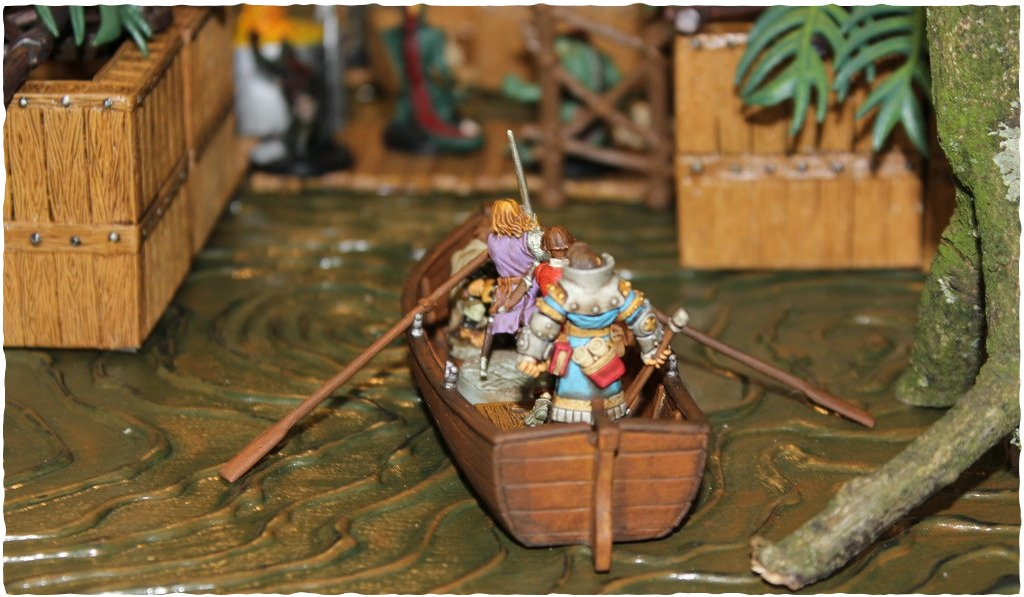
\includegraphics[width=0.4\textwidth]{images/Approaching-the-lizardmen-village-540871537_mod.jpg}
	\caption{Approaching the lizardmen village}
	\label{fig:Approaching-the-lizardmen-village-540871537}
\end{figure}



	%!TEX root = ../crimson_throne_book_main.tex
% 2015-06-30
The heroes have located the lizardfolk settlement in the Mistmoors. As they approach, they notice that the scaly creatures are all distracted by something:\hyperref[fig:Mistmoor-lizardfolk-sacrificing-centaur-543065415]{ they are all staring in the direction of the beating drum } . Balian seizes the opportunity to glide the boat right up to the pile huts. Puk jumps out of the boat and climbs the first building they pass, while Quint calls out with a friendly voice: "Here, catch!" He throws then end of a rope to the closest lizardman. Surprised by the sudden arrival of armed pinkskins, the creature shouts out in a language none of the companions understands, grabs his club and starts bashing his shield with it vehemently. The entire tribe picks up his war cry and looks ready for battle. \\

\begin{figure}[h]
	\centering
	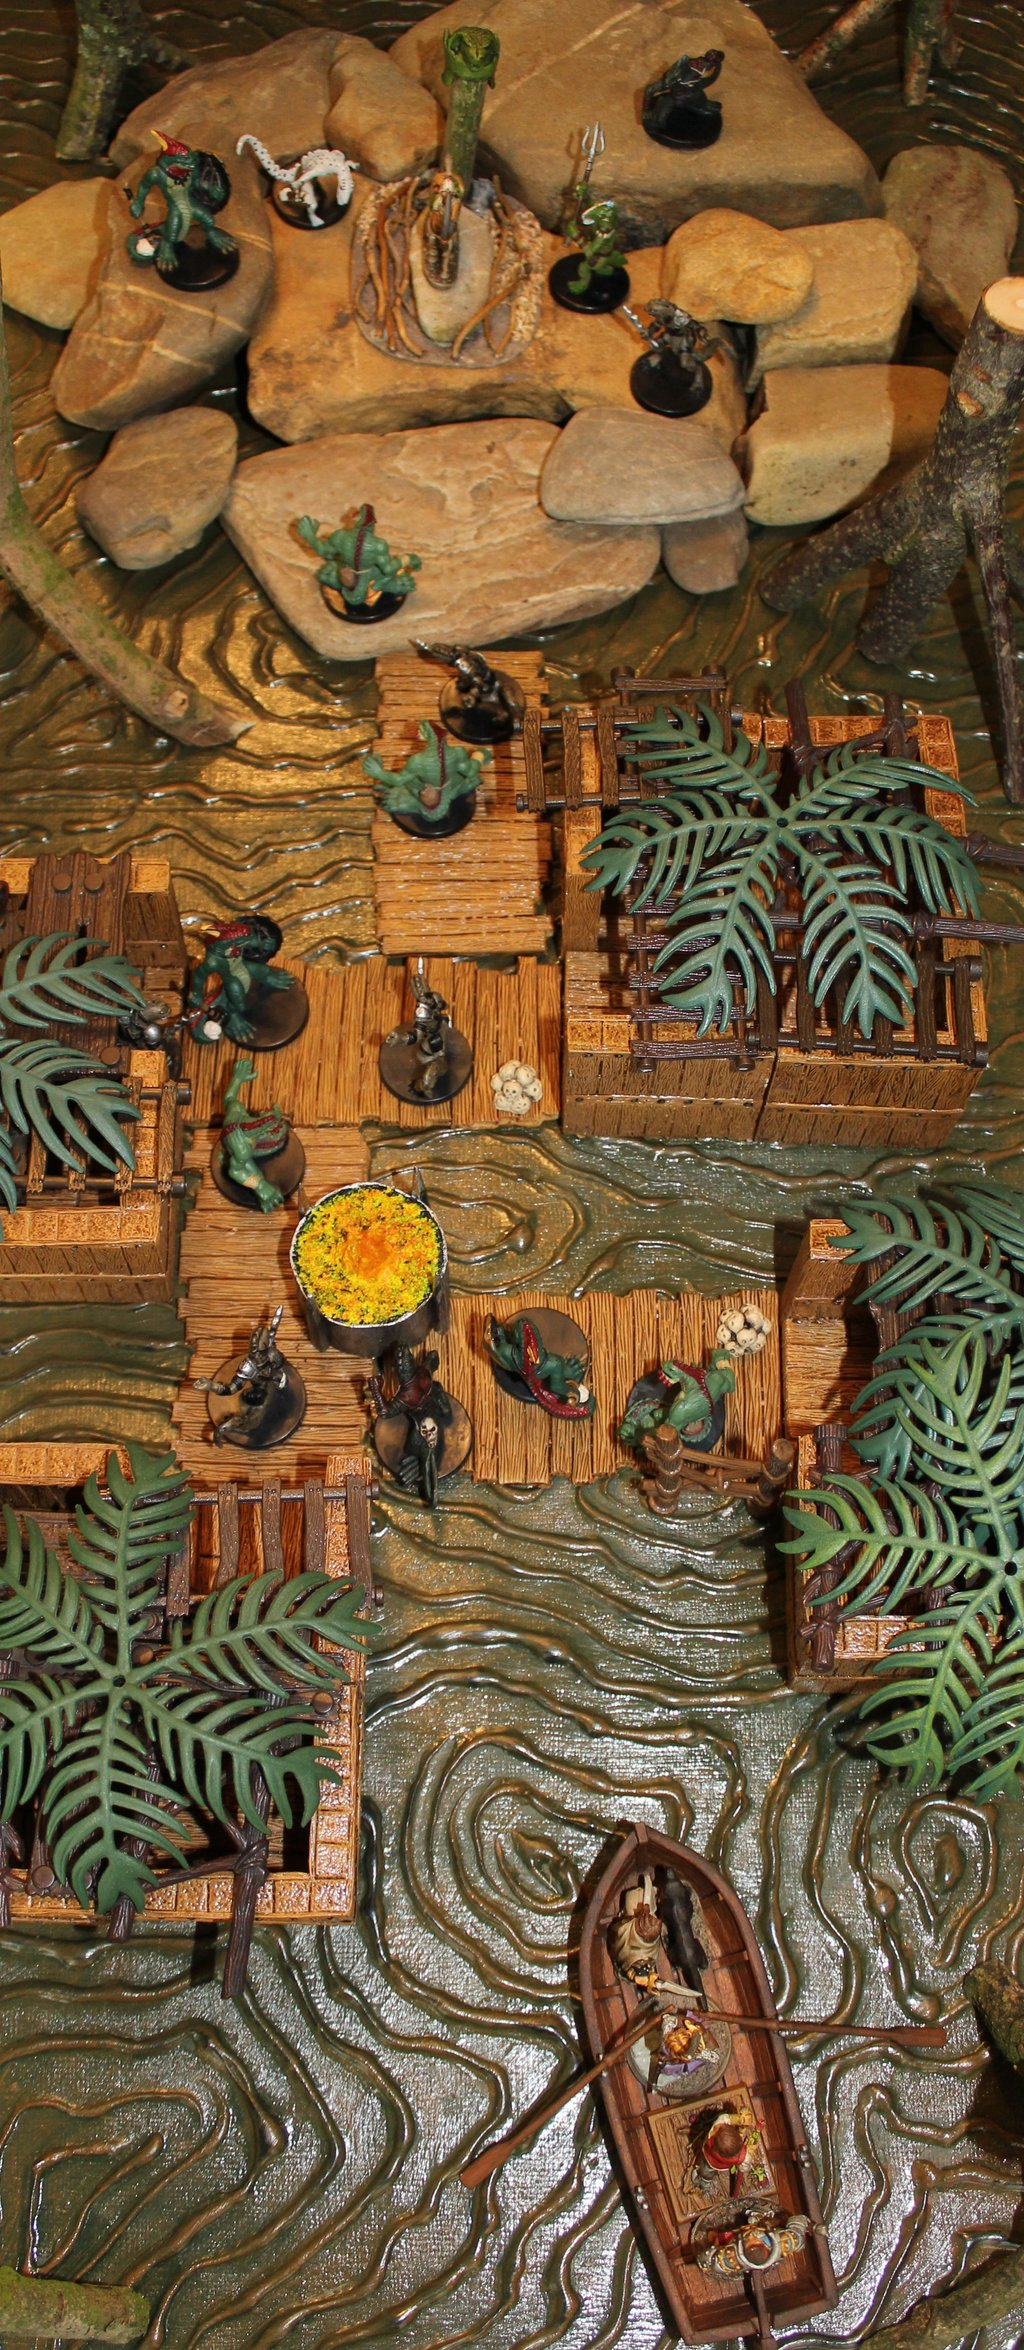
\includegraphics[width=0.39\textwidth]{images/Mistmoor-lizardfolk-sacrificing-centaur-543065415.jpg}
	\caption{Mistmoor lizardfolk sacrificing centaur}
	\label{fig:Mistmoor-lizardfolk-sacrificing-centaur-543065415}
\end{figure}

While Quint realizes that he knows no language to successfully communicate with these creatures, his friends jump into battle and quickly take down a number of lizardfolk. Sjo notices a mass of rocks beyond the pile houses, where a fair number of scaly creatures have gathered. He summons a mighty fireball, killing four of them and wounded two others. Puk, Balian and Spyder meet with more resistance as they face some lizardmen wearing hide armor and shields, obviously warriors of some kind. Quint trips one of them and again the bard calls out for a seize-fire, but to no avail. By now the chieftain joins the fight, while the white-scaled shaman summons an owlbear to slow down the heroes' advance.\\

Quint attempts to capture the chief in a {\itshape cacophonous call} , but the creature is not affected, and Sjo fails to dispel the owlbear. Meanwhile Balian and Spyder pick off the last 'common' tribesmen, so only the chief, shaman and the summoned monster remain. The ranger feels that the shaman tries to freeze him in place, but bites back and resists the  {\itshape hold person} . Quint finally manages to control the battlefield by nauseating the leader and his medicine man with two successful  {\itshape cacophonous calls} . Both of them slip into the murky waters, giving the companions the time to take out the owlbear and heal their wounds. Tied to some kind of sacrificial altar is Mirala, the missing centaur girl. Furian, the pixie, blinks out of invisibility and starts babbling away while Sjo unties the horsegirl. Mirala claims to be confused by the tribemen's behavior. They rescued her from the quicksand, took her to their village and treated her with respect, although she could not communicate with them. Today, they suddenly grabbed her and tied her to this pole, but she doesn't understand why. Sjo wonders if they were planning to bleed her out in a sacrificial ceremony, but Puk realizes they were literally trying to offer her to the creature that suddenly rears his ugly head from the swamp waters: a black dragon! Before they can react, the dragon spews a stream of biting acid on Sjo, Spyder, Quint and Furian. The little pixie goes down. Next the black-skinned retile sinks his teeth in Quint's flesh. At the same time the lizardfolk chieftain and shaman climb out of the water again. Puk and Sjo confront the dragon, while Balian and his dog fight back the two lizardmen. Quint distracts the enemies with his {\itshape satire} and hands his  {\itshape wand of cure serious wounds} to Mirala, who support the fight with some well-placed healing. During her medical work she sings an inspiring song which lightly boosts the companions fighting skills. Balian's greatsword cuts deeply into the chief's flesh, but his shaman sidekick heals him again. Fortunately, our ranger friend is on a roll and with a critical hit he takes down the fierce lizardman. The shaman flees into the water and swims to the dragon's side. This monster seems to have overestimated his own power: he does wound his opponents badly, but Mirala's healing keeps them on their feet and their weapons hit him time and again. The shaman heals him enough to continue fighting, but when Balian delivers another critical blow, the dragon decides not to tempt fate any longer and escapes, barely alive. The lizardfolk medicine man quickly follows his 'god', leaving the companions victorious. Sjo can bring back Furian from the brink of death, while Balian finds that the alter is covered in red toadstools: blood cap mushrooms! Hundreds of them!\\



	%!TEX root = ../crimson_throne_book_main.tex
% 2015-07-18
The companions fill a bag with red mushrooms and then seek their way out of the swamps. Although Furian is very happy to see Mirala alive, he has a troubled heart when he tells her that her brother avenged her 'death' by killing over a dozen of his kin. Mirala feels guilty about her part in this tragedy, as it was her irresponsible behavior that triggered her brother's madness. She wants to confront her brother alone, so the heroes accompany Furian to the pixie court, while the centaur girl makes for Pointer's Rock.\\

Pixie king Tirmando is pleased to hear that Mirala survived, but no amount of good news can sway his mournful mood. Still, he remembers his promise to the adventurers and hands his green-leaf cloak to Puk as a reward. This wonderful cape functions as a {\itshape cloak of resistance} , but it also allows the wearer to  {\itshape dimension door} once per day. The king invites his guests to spend the night at his court before they return home tomorrow. Later that evening Mirala arrives, explaining that her brother is distraught about his own heinous deeds and has decided to leave the vale to seek atonement for his sins. \section{Level up: level 7}

\section{17-19 Erastus 4708}

The next morning the companions head back to Korvosa. On the evening of the 18th Zellara's ghost appears to them from her Harrow deck to do another reading. She removes the nine {\itshape book} cards from the deck and has everyone draw one. Sjo evokes a healthy dose of laughter when he draws the  {\itshape idiot} , which Zellara interprets as a warning not to be too naive. Quint goes for the  {\itshape inquisitor} , who accepts only the truth. Zellara says that Quint will be instrumental in uncovering an important hidden truth. Balian draws the  {\itshape raksasha} as a warning not to be manipulated. Balian should be careful not to act differently than what his true nature prompts him to do. Puk's card is the  {\itshape vision} : he will meet a man whose insanity and genius will be intertwined. Next Zellara reshuffles the cards and lays them out for each of the companions. In Sjo's present she finds the {\itshape crows} , who represent a group of dangerous people who violently take possession of what is not theirs. The  {\itshape desert} is in his future, as a sign of a harsh environment in which he will have to survive. Quint has the  {\itshape foreign trader} in his past, representing a hidden truth whose unveiling will surprise some and shock others. The future reveals the  {\itshape uprising} : a leader will be overthrown, but it remains unclear which part Quint will have to play in this. Puk has the  {\itshape tangled briar} in his past. Bad events in his younger days defined his path, but set him on a journey towards hope. Puk's future reveals the same card he picked in the choosing, the  {\itshape vision} . Zellara concludes from this that the mad genius will play a key role in days to come. Balian's fortune also shows important facts about the past. The  {\itshape empty throne} signifies a great loss that still defines his life today. The  {\itshape idiot} also comes up here, indicating that Balian made a rash decision in the past and the fact that he fooled others about it will not be received kindly. The  {\itshape marriage} in Balian's present stands for big changes that are about to happen. Zellara says that the positive position of the card expresses the hope that Balian will be able to sail the waves of change and maybe even help shape them. His future is less clear, although Zellara interprets the  {\itshape forge} card as a sign that a great heat that has burned everything to cinders might be part of Balian's fate. 

	%!TEX root = ../crimson_throne_book_main.tex
% 2015-07-18
\section{20 Erastus 4708}

Late in the afternoon of the 20th the companions reach the gates of their home city. They immediately head to the university, to hand the blood cap mushrooms to professor Sirtane Leroung. She instantly sends an envoy to warn the castle. Quint feels a bit surprised, but Sirtane eases his mind by saying that the whole city is eagerly awaiting her cure. She gives him the latest issue of the {\itshape Korvosa Herald} , which has an article on the topic:  {\itshape Cure for the plague just around the corner!} . Her brother-in-law, who publishes the newspaper, insisted on it, Sirtane explains. There is also a report on the treacherous plague doctors and the quarantine of Old Korvosa. The history of Korvosa on the back is devoted to the reign of queen Domina and her son Eodred II. Puk also informs about Madam Nesia's blood which he collected after she exploded into a sea of sanguine fluid. Fortunately Sirtane has found some time to examine it. The blood clearly showed signs of residual transmutation magic of a very high order. She believes it to be a weird modification of the {\itshape simulacrum} spell, powerful magic that allows a magic-user to construct an illusionary double of someone from snow and ice. This spell requires a very accomplished caster and costs thousands of golden sails in ingredients. In Nesia's case blood was used instead of ice and snow, which is clearly a more powerful ingredient, but the fact that Nesia had no memories and became sick and died, shows that the spell that created her had not been perfected yet. Mages who master this level of magic are extremely rare, in Korvosa they can probably only be found in the Acadamae, Sirtane muses. By the time Sirtane has finished her expos\'e on Nesia's condition, her messenger returns from the castle. He says that the queen has ordered her and her family, and also the companions, to come to the castle tonight, where Ileosa will address her people for the first time in weeks. Our friends decide to return home to bathe the dust of travel from their skins and dress up for the occasion.\\

Upon arriving at the villa the companions notice that the three kids are nowhere to be found. There is no note either. Sjo is worried that the children got sick again; after all, it's been ten days. A sudden knock at the front door pulls the healer from his contemplation. There is a beautiful Varisian woman at the front door who insists on talking to Balian. She introduces herself as Ravenna and Sjo sees that she is not alone, another man is waiting for her in the street. Balian joins the Varisians and agrees to go with them, without telling his friends where he is going. It looks important, as the ranger is willing to give up a visit to the castle for it. Puk decides to follow the ranger stealthily and tails him to a house in Thief Camp. The building looks well guarded, so the halfling sees no easy way in and returns to the villa to prepare for the queen's speech instead. Unlike Balian he does not want to pass an opportunity to gaze on the beauty of the queen.\\

In their smartest attire Sjo, Puk and Quint go to the castle, where a small crowd of the city's finest has already gathered. Everyone is quite curious. At the foot of the grand stairs up the mastaba Puk spots Cressida Kroft. She wonders as well what this meeting is about and points out that there are a lot of Gray Maidens present. The Castle almost looks like a fortress preparing for battle.\\

The guests are allowed into the throne room where the waiting continues. The room buzzes with impatience when the queen suddenly appears out of thin air, flanked by the commander of her Gray Maidens and a heavy, bald man - clearly a spellcaster. His robes cling tightly to his firm body. Ileosa is wearing a new crown with spikes that look like giant shark teeth. While everyone falls silent, Quint calls out: "Queen Ileosa, it has been too long, it is good to see you again." The queen returns his words by briefly piercing him with her gaze, which she then sends over the other guests in the room. She beams with confidence when her lips curl into a smile and she addresses the crowd:\\

"My dear citizens, there is light at the end of the tunnel. Hold on a bit longer and the plague that fell over us will be a thing of the past. We have a cure!\\

I know, our recent path has been riddled with hardship and challenges. There were many casualties and fear overtook us all. But rest assured, the nightmare will soon be over. The university of Korvosa has developed a medicin. Just a few more days and life will rule the streets again instead of death.\\

Korvosa is indeed a beautiful city and many envy her for her riches and pleasures. They try to crush us with riots, but we resist! They try to starve us, but we survive by sheer will. They try to cut us down with disease, but we arise stronger than ever. The enemy comes to us in many guises, as opponents or as allies. Treachery runs deep sometimes. The physicians who came to the city, weren't healers who were trying to make us better, but the true architects of the plague itself! But we triumphed over them all!\\

Still, all these attacks have taken a heavy toll. Thousands of citizens fell to the disease, everyone of us has lost friends or family. The Korvosan Guard is crippled and the Sable Company is broken by numerous losses. None of these troops have the strength left defend our city properly. So I proclaim that henceforth the Gray Maidens are the new protectors of the realm and their commander Sabina Merrin is the general of all military forces in Korvosa."\\

A wind of discomfort waves through the crowd, but Ileosa is not finished yet. She hails the heavy man to her side: "This gentleman is Togomor, my new advisor who will take up the duties of castle seneschal from now on.\\

I have also decided to dissolve the Sable Company and merge their depleted numbers with the Guard, making one whole from two halves. Commander Endrin of the Sable Company, please approach!"\\

The crowd is baffled as Marcus Thalassinus Endrin steps forward. Quint uses the consternation to utter the words of a {\itshape detect magic} spell and sees that the queen, Merrin and Togomor all bear powerful magic. Especially the crown radiates a strong glow. In the meantime Endrin makes his way to the podium. "Commander, I hereby strip you of your command and ask you to surrender your badge of honor."\\

As Endrin does so, he trembles. He reaches for his badge, but instead of handing it over, he throws it at the queen, cutting her left cheek. Everyone, including Ileosa, is shocked into paralysis for a few moments, long enough for Endrin to bellow out: "Your shameful reign ends now! Korvosa will be free again!" At that point his other hand appears from under his cloak, firmly grasping a loaded crossbow. He aims at the still-locked queen and pulls the trigger. His bolt strikes Ileosa straight in the temple: a deadly shot!\\

Yet the queen does not fall.\\

She doesn't even tremble.\\

With incredible speed she regains her composure and yanks the bolt from her head. Before the blood from her wound has time to trickle down her cheek, she rushes over to Endrin. With her free hand she grabs the man by the throat and lifts him off the ground. Her other hand wields the bolt as a dagger, which she hammers between Endrin's eyes. The commander's lifeless body tumbles to the floor, as Ileosa turns to the crowd and cries out: "This shall be the fate of all enemies of Korvosa! Mark well his death! All traitors will suffer the same fate!"\\

A second later Togomor steps forward, laying his hand on Ileosa's shoulder and teleporting her out of the throne room. Sabina Merrin orders everyone out and her Gray Maidens start pushing the crowd towards the exit. Field Marshal Cressida Kroft is stunned and horrified by what she has seen. She takes the companions to her office in the citadel to speak with them freely. Her gut tells her to step down from office, but she fears that a Gray Maiden puppet will replace her then, so she decides against her gut feeling. She hopes that by complying with the queen, she can exert the largest possible amount of control to see her soldiers safe. Quint is angry: Endrin's peaceful approach has only lead to the man's untimely death. The bard feels like the city is slowly being murdered in front of his eyes.\\

A knock on the door disrupts the conversation. A guard from the Longacre Building bears a letter for the Field Marshal. It was given to him by a boy who was arrested for escaping from Old Korvosa. Kroft thanks him and starts reading. "This comes from Vencarlo Orisini," she says, "it looks like he is looking for you. Here, read it."\\



	%!TEX root = ../crimson_throne_book_main.tex
% 2015-07-18
Quint takes the note from her.\\

 {\itshape "Dear Cressida}  It has been a while since we have talked. Since the Gray Maidens locked off Endrin Island from the rest of the city, I have been stuck here. At least officially. Let's just say that one does not simply walk out of Old Korvosa these days.\\

Things have been chaotic here. The plague has ravaged the district. No family has been spared. Without the support or hope from the city's churches many people have fallen prey to despair or disorder. Several buildings lining the quays have been torched and gangs have taken over the streets. Some madman has crowned himself 'emperor of Old Korvosa', you might have heard of him, Pilts Swastel, the deranged owner of a detestable and perverse theatre, Exemplary Execrables. Fort Korvosa is the only place that is still safe, for that is where the Arkona's rule. But the rest of our district is in dire straits.\\

Anyhow, Old Korvosa might very well be the garbage dump of Korvosa, it is in the city's filth that one finds the most surprising information. I have uncovered some vital clues regarding the queen. You know that I have distrusted her from the very beginning. I do not grasp the full picture just yet, but I fear that dark magic is at work here, possibly a pact with a devil of some sort.\\

Can you get in touch with our new friends? You know, those young heroes who have helped out before. I have not been able to follow their adventures of late. Are they still safe and in good health? Can you ask them to pay me a visit? The likes of them should have no trouble crossing the Narrows of Saint Alika to Old Korvosa, despite the quarantine. They might even be safer here than on the mainland, after all, there are no Gray Maidens here. The queen has left Old Korvosa to rot, but at least this frees us from her choking grasp.\\

I greet you cordially and remain your faithful friend,\\

you know who ..."\\



	%!TEX root = ../crimson_throne_book_main.tex
% 2015-07-18
Great session here! Once again you're proving your ability to beautifully interweave the general plotline with the characters' background and personal relations. Very much looking forward to Adventure 3!\\



	%!TEX root = ../crimson_throne_book_main.tex
% 2015-07-19
BALIAN, CG Male Human ranger 7 (urban ranger)  Init Senses  AC touch flat-footed  hp  Fort Ref Will  Speed  Melee  {\itshape greatsword +1} (two handed) +13/+8 ((two handed) 2d6+8/19-20)  Melee  {\itshape masterwork dagger} +13/+8 (1d4+5/19-20)  Ranged  {\itshape masterwork longbow (composite/strength rating+4)} +11/+6 (1d8+4/x3)  Base Atk CMB CMD  Ranger Spells  1st  {\itshape lead blades, longstrider}   Abilities  Special Qualities  Feats  Skills  Possessions  {\itshape greatsword +1} ;  {\itshape ring of protection +2} ;  {\itshape mithral breastplate +1} ;  {\itshape amulet of natural armor +1} ;  {\itshape belt of physical might (+2 str/con)} ;  {\itshape cloak of resistance +1} ;  {\itshape wand of cure light wounds} ; masterwork dagger; masterwork longbow (Composite/Strength Rating+4)  Favored Community Korvosa (Ex)  Favored Enemy (Human +4, Undead +2) (Ex)  Trapfinding (Ex)  Push Through (Ex) Trained actor  Child of the Streets  Reactionary SPYDER, dog companion level 7, N Medium animal  Init Senses  AC touch flat-footed  hp  Fort Ref Will  Speed  Melee  Abilities  Base Atk CMB CMD  Feats  Skills  Devotion  Possessions  {\itshape amulet of natural armor +1} ;  {\itshape studded leather barding +2}  ---\\

PUK, CG Male Halfling rogue 7 (swashbuckler)  Init Senses  AC touch flat-footed  hp  Fort Ref Will  Speed  Melee  {\itshape silver short sword +2 (small)} +12 (1d4+2/19-20) and off-hand  {\itshape short sword +1 of shock (small)} +11 (1d4+1+1d6/19-20)  Melee  {\itshape masterwork sap (small)} +12 (1d4 non-lethal/x2)  Ranged  Ranged  Base Atk CMB CMD  Atk Options  Abilities  Feats  Skills  Possessions  {\itshape small short sword +1 of shock} ;  {\itshape small silver short sword +2} ;  {\itshape studded leather +2 (small)} ; shortbow (Small); halfling sling staff (halfling); small masterwork sap,  {\itshape amulet of natural armor +1} ,  {\itshape ring of protection +1} ;  {\itshape cloak of the Pixie King (+2 on saves, Dimension Door 1/day)}  Sneak Attack (Ex)  Bleeding Attack (Ex) Fast-Talker  Personal Addiction ---\\

QUINTILIAN (QUINT), CG Male Human bard 7 (court bard)  Init Senses  AC touch flat-footed  hp  Fort Ref Will  Speed  Melee  {\itshape short sword +1 of frost} +9 (1d6+3+1d6/19-20)  Melee  {\itshape longsword} +8 (1d8+2/19-20)  Melee  {\itshape masterwork whip} +9 (1d3+2)  Melee  {\itshape sap} +8 (1d6+2)  Ranged  {\itshape shortbow} +8 (1d6/x3)  Base Atk CMB CMD  Known Bard Spells  3rd  {\itshape glibness, haste}   2nd  {\itshape cacophonous call, gallant inspiration, heroism, mirror image, pyrotechnics}   1st  {\itshape cure light wounds, expeditious retreat, innocence, memory lapse, silent image, timely inspiration, touch of gracelessness, ventriloquism}   0th  {\itshape detect magic, ghost sound, light , lullaby, mage hand, message, open/close, prestidigitation, read magic}   Abilities  Feats  Skills  Possessions  {\itshape short sword +1 of frost} ;  {\itshape chain shirt +1} ;  {\itshape buckler +1} ; longsword; masterwork whip; sap;  {\itshape wand of feather step} ;  {\itshape wand of cure light wounds} ;  {\itshape wand of mage armor} ; Shortbow;  {\itshape amulet of natural armor +1} ;  {\itshape Wand of magic missile (CL 3rd)} ;  {\itshape Scrolls of levitate, gentle repose, false life, knock} ;  {\itshape Dust of appearance} ;  {\itshape ring of fire resistance (10)} ;  {\itshape ring of protection +1} ;  {\itshape cloak of resistance +1} ;  {\itshape Belt of Physical Might (+2 Str/Con);  [i]Key-Lock Killer's bell}  Bardic Performance  Versatile Performance (Comedy / Oratory) (Ex)  Countersong (Su)  Distraction (Su)  Fascinate (Su)  Heraldic Expertise (Ex)  Satire  Mockery (Su) Trained actor  Fast-Talker  Child of the Street ---\\

SHAOBAN (SJO), LN Male Human oracle 7  Init Senses  AC touch flat-footed  hp  Fort Ref Will  Speed  Melee  {\itshape cold iron mace +2 (heavy)} +11 (1d8+5)  Base Atk CMB CMD  Known Oracle Spells  3rd  {\itshape cure serious wounds, dispel magic, fireball, prayer}   2nd  {\itshape cure moderate wounds, hold person, remove paralysis, resist energy, restoration (lesser), weapon of awe}   1st  {\itshape burning hands, comprehend languages, cure light wounds, magic weapon, protection from chaos, remove fear, shield of faith}   0th  {\itshape create water, detect magic, purify food and drink, read magic, spark, stabilize}   Abilities  Feats  Skills  Possessions  {\itshape cold iron mace +2 (heavy); ring of protection +1; full plate +1; amulet of natural armor +1, cloak of resistance +1, belt of giant strength +2, wand of cure light wounds, wand of remove disease} ; buckler Clouded Vision  Flame Mysteries  Touch of Flame (Su)   Molten Skin (Ex)  Wings of Fire (Su) Trained actor  Child of the Streets  Ease of Faith 

	%!TEX root = ../crimson_throne_book_main.tex
% 2015-07-25
The party decides to get into Old Korvosa by boat from the other bank of the Jeggare River. Trail's End, outside of the city walls, seems like the perfect spot to get across. Tayce Soldado, Brienne's mother and guard Grau's sister-in-law, lives there, so maybe she can help them find suitable transportation. The companions gather their gear and leave the villa. While making their way through Midland to the High Bridge, they suddenly see three scared Korvosans fleeing from something. Rounding the corner the companions come upon the source of this panic: seven Gray Maiden are locked in mortal combat with three Sable marines. The three black-clothed soldiers are obviously outmatched. Quint addresses the officer of the attacking force, questioning her violent actions and trying to get her to stand down by {\itshape fascinating} her, but he only succeeds in isolating her from the combat while her squad continues pressing the unfortunate members of the Sable Company. Balian's instincts tell him to interfere, but Quint cautions him: fighting the Gray Maidens will only result in outlawing the companions as well. So our friends watch with horror how the ironclad female warriors butcher the marines. The officer explains that Sable Company members have been declared 'public enemies'. These soldiers refused to surrender, so they were put to the blade. As the Gray Maidens march off, Sjo recognizes the dead marines from his days in the Sable company's stables. He feels torn, but has to agree with Quint that stepping in would have compromised their own mission. Quint also adds that killing Gray Maidens is not the solution, after all, these women are just following orders. Moreover, the companions cannot take on the complete force of Gray Maidens by themselves, as there are rumored to be 500 of them in the city and their numbers seem to increase every day. With a heavy heart the young friends continue their own quest. Tayce is relieved to see Sjo: her daughter still hasn't recovered from the plague, so the healer digs up his {\itshape wand of remove disease} to cure the girl. In return Tayce convinces her neighbor Jarend to take the companions across the river. The skilled fisherman is glad to assist and drops the heroes on the easternmost quay of Old Korvosa, cleverly avoiding the Gray Maidens sloops that patrol the water. Quint leads his friends straight to Eel's End. The 'entertainment center' is still running, although there are a lot less visitors than before. No surprise, since Old Korvosa is cut off from the rest of the city. Almost all patrons are sporting a strip of red cloth bound around their right arm. Quint quickly learns that they are the {\itshape emperor's} 'men', though the word thugs would suit them better. So Vencarlo's letter spoke true: Pilts Swastel, the crazy owner of obscene  {\itshape Exemplary Execrables} theater, has become the self-proclaimed ruler of the quarantined district. Quint boards the  {\itshape House in the Clouds} , the brothel where Yuuna works, and asks her boss about her. Madame Halvara claims that she hasn't seen the Vudran girl in five days. She recommends that the bard talks to Danarella, who is Yuuna's best friend. Perhaps she knows more. Sjo's ears already glow red as he thinks of the pretty redhead who helped him lose his virginity, but it looks like she is 'occupied' with one of the emperor's men for the moment. The Shoanti also picks up that the brothel's Madame does not seem overly pleased with Pilts Swastel's mob crowding her establishment. When he questions her about it, she whispers that the emperor's men act as if they own the place and pay only a fraction of the normal rates to get their kicks. But they are the only business Eel's End sees these days. The companions figure that the emperor is probably the best source of information in Old Korvosa at the moment, so Quint uses {\itshape fasinate} and  {\itshape suggestion} on one of his cronies. The ruffian, whose name is Patrick, agrees to take the party to see his boss. As he leads the way through the streets, his gang of thugs notice a drifter who is coughing badly and has trouble standing. Sjo immediately makes out that the stranger is suffering badly from the plague. "There's one of those filthy infected!" the thugs scream as they brandish their short swords and storm the unfortunate soul, quickly slashing him down without mercy. "That is the way we deal with the diseased in Old Korvosa", Patrick laughs. As they approach the former theater, the companions see that the playhouse has partially burnt to the ground, a theme that seems to run all over the island recently, just like the heaps of rotting cadavers in the streets. Several walls are covered in graffiti with slogans like "Gods bless the emperor", "Swastel is the man" or "Pilts to Power", and depictions of a bloody guillotine and heads flying about. Most houses in the area are boarded up tightly, others look abandoned with their front doors kicked in. Pilts Swastel's new 'palace' consists of a block of buildings that escaped destruction, right next to his erstwhile theater. Patrick knocks on the door of a small corner house and takes the companions past the guards up rickety stairs inside. Through a splintered hole in the wall he proceeds them over a rope bridge to a second building and then over another bridge to a huge open-air balcony clinging to the south side of a large tenement. The terrace is shielded from the elements by a brightly colored canvas roof that extends over the area like a dome, held in place by a wooden framework. The balcony itself contains two features of note. The first is a high backed chair that looks like a poor man's version of the Crimson Throne itself. Directly west of the throne stands an intimidating device, a tall guillotine of carved wood and bone, its blood-spattered base depicting grasping demonic feet and the housing that holds its glittering blade looks like a leering demonic face. Puk recognizes the apparatus as the Demon's Maw from Galt, one of Swalts' most prized possessions from his freak show museum. Flies hovering over a nearby basket leave no doubt to its content: severed heads. Lazily relaxing in the throne's red cushions is a familiar figure. He looks even more hideous than he did when they met him three months ago. His eyes have fallen back in his skull, his pockmarked face indicates that he survived a bout with the plague, but not unscarred. He is dressed in a threadbare fur-trimmed crimson cloak and a cheap crooked crown, both pieces from his extensive collection of stage costumes and attributes. Pilts Swastel looks more like a vagrant king than actual royalty. His gaze betrays more than a touch of madness, but when he speaks the almost hypnotic pattern of his voice explains how he managed to gather the desperate and cruel to his banner. The toughest of the Old Dock thugs have made it to his personal bodyguards, guarding all corners of his throne. Staring from the hole in an executioner's mask is a sturdy gnome. Since the second eye-hole in the mask has been sewn shut, this can only be Swastel's tongueless, one-eyed sidekick, Jabbyr.\\

The emperor of Old Korvosa remembers the companions and welcomes them to\hyperref[fig:Audience-with-the-Emperor-of-Old-Korvosa-548846605]{ his court } . He saw them perform at the Marble Dome and was especially taken with their inspired alteration of the opera's final scene, with a genuine fight and real blood spattering the stage. When he inquires why the party has come to his island, Quint informs him that things on the mainland are getting out of hand. The bard recounts the story of what just happened in Castle Korvosa, using  {\itshape silent image} and  {\itshape ventriloquism} to depict the scene of queen Ileosa killing the commander of the Sable Company. Swastel loves it and already envisions a new play in which commander Endrin's sexual relationship with the queen ends in his death at her corpulent advisor's hands. There should definitely be room in it for a threesome with Sabina Merrin as well, he muses. \\

\begin{figure}[h]
	\centering
	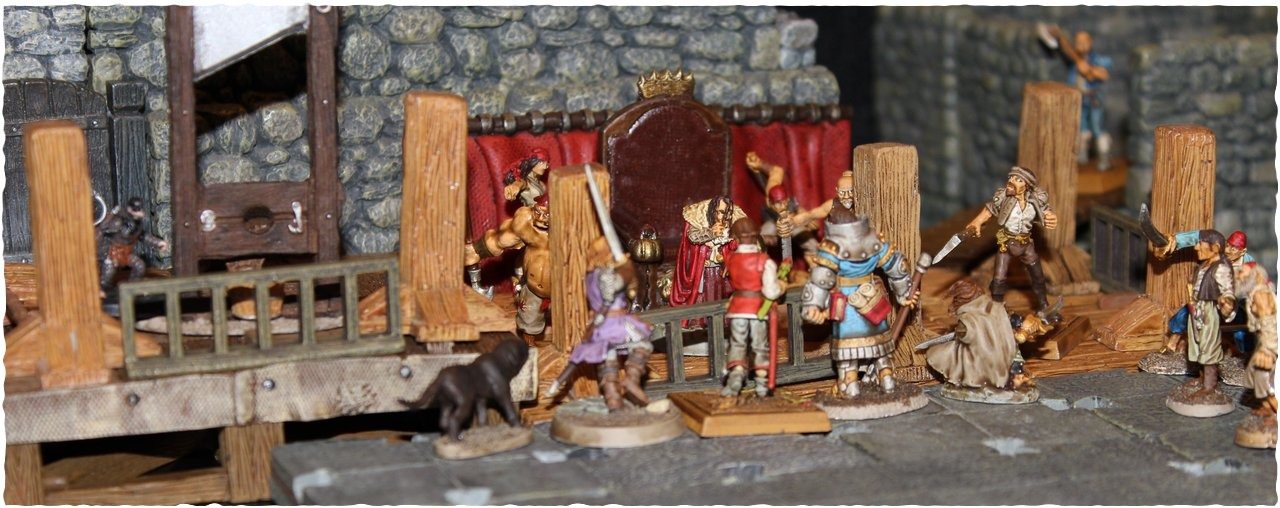
\includegraphics[width=0.4\textwidth]{images/Audience-with-the-Emperor-of-Old-Korvosa-548846605_mod.jpg}
	\caption{Audience with the Emperor of Old Korvosa}
	\label{fig:Audience-with-the-Emperor-of-Old-Korvosa-548846605}
\end{figure}

Next Quint changes the subject to Rolth, who is supposed to be hiding in Old Korvosa. He does his best to portray the necromancer as a great threat to the emperor's rule, but also admits that Rolth kidnapped some children who need rescuing. "So in fact you come to me seeking my assistance, hmm, let's see ..." Swastel sighs before mumbling the words of a {\itshape detect magic} . "I do like that belt you're wearing, young bard", he smiles at Quint. "It would make a handsome tribute to my person, as well as an acceptable payment for my services." The emperor makes his exorbitant demand with an air of self-evidence; emanating that he will not take 'no' for an answer. Being from a humble background, Quint has had to earn every one of his possessions through hard work and understands their value. He feels insulted and bellows at the emperor. Then things go fast: the emperor's bodyguards jump forward, stun Quint with a well-placed punch and grapple Balian. Sjo tries to freeze one of them with a  {\itshape hold person} , but his magic is resisted. Balian struggles out of the brute's grasp, but the emperor whispers a  {\itshape charm monster} and sways the ranger not to fight. "Just give me my prize and get to your knees, young bard. My court, my rules! Now don't be stupid!" Swastel grins at Quint. Puk realizes that complying with the emperor's wishes is the only tactic to get out of this mess alive, so he frees Quint' belt from the stunned bard's waist and throws it at Swastel's feet. The next moment one of the emperor's brawlers forces Quint on his knees and the fight is over. Pilts Swastel girds on the shiny belt and suddenly seems bored with his guests. "I'll see what I can do about this Rolth character. You are dismissed", he blurts out. Not wanting to overstay their welcome, the companions take their leave. A displeased Quint vows to himself this is not over yet. 

	%!TEX root = ../crimson_throne_book_main.tex
% 2015-07-25
The companions' next destination is Yuuna's flat. Balian easily picks the lock and finds a small, but colorful room. There is no trace of Yuuna, there are no signs of a struggle, only the back window has been forced open. Nothing else is of any help to the young men, so they return to Eel's End to talk to Yuuna best friend, Danarella. The redhead has no idea where her Vudran colleague disappeared to, although she hopes her friend is okay. She might have fled to the mainland, but Danarella suspects that Yuuna would never do that without informing her. Maybe Yuuna's {\itshape stalker} knows more, she muses. She explains that Yuuna had a 'fan', a man who was probably in love with her and who regularly escorted her home after work. They jokingly called him her 'stalker', although he was quite a respectable man, a trainer at the Endrin military academy, called Janros Rainwater. Endrin military academy is a whitewashed building that acts as barracks and training grounds for a small garrison of both Korvosan guards and Sable Company trainees. This place does not just only drill soldiers and teach them new tricks and tactical insight, it also serves as a breeding ground for good relations between the Guard and the Sable Company. The trainees act as liaisons between the two military forces, allowing for joint operations and continued mutual support. The academy's location within the old wall of Fort Korvosa, at the foot of Garrison Hill, provides a more serene scenery than the chaotic streets of Old Docks and the cramped alleys of Bridgefront. Although there are signs of plundering and destruction here as well, they are less frequent and there are no decaying bodies on the ground or thugs about.\\

Double doors bar the entrance to the academy. A note has been nailed in the wood: {\itshape Academy closed - No entry} . Balian knocks loudly. The only reaction is a dog that starts barking inside, but no one answers the call. Since this building is so close to Vencarlo's house, the companions want to pay the fencing master a visit first. Maybe he knows his colleagues in this training center, so he might facilitate their access. Two blocks away stands Vencarlo's famed sword school, or at least, that is where it used to stand. The once-proud Orisini Academy is no more: the training facility has recently burnt to the ground. Fortunately, Vencarlo's living quarters still stand, nestled in the other corner of the compound. Puk's quick eyes pick up a line of smoke coming from the chimney, so the fencing expert is at home! When Balian knocks on the door, it clicks open from the impact of his blows. Why would Vencarlo leave his door unlocked? The companions draw their weapons and carefully enter the building. The ground floor is empty. If Vencarlo is still here, he is probably resting upstairs ... and if he isn't, the bedroom might just be the best place to find a trace. The stairs lead to a personal training room with a burning fireplace and two practice dummies in the far corners, to either side of the hearth. The exposed rafters give the room an open feel. There is one more door in here which can only lead to the bedroom. Puk's sixth sense warns him of a danger as\hyperref[fig:Red-Mantis-attack-in-Vencarlo-s-house-548844795]{ two shadows drop down from the beams above } . Their weird armor resembles the carapace of a scarlet insect and their blood-colored ant-like helmet completes the picture: Red Mantis assassins! \\

\begin{figure}[h]
	\centering
	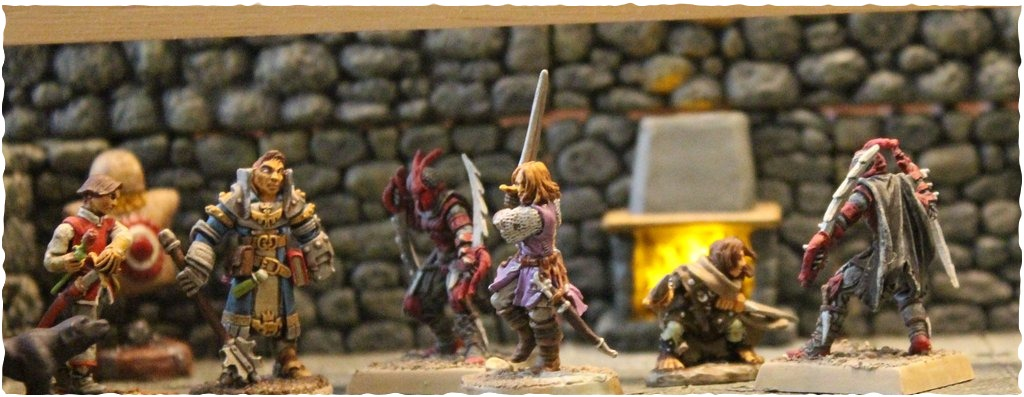
\includegraphics[width=0.4\textwidth]{images/Red-Mantis-attack-in-Vencarlo-s-house-548844795_mod.jpg}
	\caption{Red Mantis attack in Vencarlo's house}
	\label{fig:Red-Mantis-attack-in-Vencarlo-s-house-548844795}
\end{figure}



	%!TEX root = ../crimson_throne_book_main.tex
% 2015-08-01
The first assassin uses the element of surprise well by slicing into Quint's flesh with his curved, serrated blade. His comrade never gets the chance, however, as Balian brings down his greatsword in a devastating arch, tearing apart the man's carapace armor. When the heavily injured hitman tries to stumble out of the way, the ranger follows up with another bloody sweep, finishing off his opponent once and for all. As his corpse hits the floor, the room is suddenly filled with a red mist. The first trained killer realizes that newcomers aren't simple students of the Orisini Academy and vanishes from view. The next moment a giant real-life red mantis appears behind Balian. The ranger easily deflects the insect's claws and continues his deadly attacks, quickly chopping the creature down. Meanwhile Puk reaches into his pocket and draws out some {\itshape dust of appearance} , which he blows into the air, making the invisible assassin reappear. The opponent now finds himself cornered and summons four  {\itshape mirror images} , but facing overwhelming odds, this act only prolongs his suffering. He manages one more feeble hit, before being overrun. As he falls down, more red mist arises and the companions notices that both assassins' corpses have completely disappeared, as if they were never there. So these are the dreaded red mantis? By the gods, how they failed to live up to their reputation! Sjo suggests using Vencarlo's house to rest up, the hour is growing late and tomorrow promises to be a rough day. At the same time they can wait here for the fencing master to come back home. The heroes quickly scan the building and discover a hidden lockbox in Vencarlo's closet. It contains a {\itshape bag of holding} , which Balian empties on the floor. The black cloak, mask, boots and gloves and the fancy rapier leave no doubt as to its proprietor: this gear is Blackjack's. So Vencarlo is the caped crusader, just as the companions expected. Sjo puts the items back in the bag and return the box to its secret compartment. Let's just hope that the old pro gets home soon, the party could definitely use an accomplished ally at its side to steer through the murky waters of Old Korvosa. \section{21 Erastus 4708}

Morning breaks and still there is no sign of Vencarlo Orisini. As the party leaves his house, Balian spots a shadowy figure trying to hide in the ruins of the burned training facility. The ranger rushes over, his greatsword blazing in the light of the morning sun. The shadow scurries backwards, stumbling over his own heels and falling flat on his bottom in the ashes. In the black dust Balian recognizes the face of one of Vencarlo's students: Amin Jalento, captain Jalento's boy.\\

"You are alive! I saw you enter that deathtrap yesterday evening ... those assassins were waiting inside. And when you didn't come out, I feared the worst!"\\

"So, what are you saying? You saw us walk into this ambush without warning us?" Quint raises his eyebrows.\\

"I'm sorry, I was hidden in that building up there, squeezed between the beams of the roof. A narrow hiding space, not easy to get out of, but a good place to remain from view. Anyway, after the master was forced to flee the day before yesterday, I've been waiting for him there."\\

"Wow, too much information at once, Amin, why don't you start at the beginning?" Sjo interjects.\\

"Of course, I apologize. You know I'm a student at master Orisini's school. I was on the island attending classes when the quarantine hit. My master was gracious enough to allow me to stay as his guest. My fellow students have all either left or died from the plague, but fortunately Vencarlo and I did not get sick. Then, two nights ago, we were set upon by five of those red killers in their ant helmets ..."\\

"Not ants, mantises actually, red mantis assassins to be exact", Quint clarifies.\\

"Gods, no ... those notorious slayers are after my master? They say the red mantis don't quit until they finish their contract. Then it's even worse than I feared. Anyway, my master held them at bay while he shouted for me to run. As I glanced over my shoulder, I saw how he took down one of them, but there were too many, so master Orisini knocked over a brazier and set the academy on fire, giving him the opportunity to flee as well. I haven't seen him since. I've been hiding, waiting for him to return. That's how I saw those two killers sneak into the house yesterday. They even lighted the fireplace, perhaps they were trying to suggest that I was in the building."\\

"And then we arrived. It didn't occur to you to shout a warning?" Balian grumbles.\\

"To be fair, I had dozed off, it was late after all. I was awakened by you knocking on the door ... before I could react, you had entered. By the time I had crawled out of my hiding place and made it to the door, I heard the sound of battle inside. When you did not come out again, I assumed you had been slain. So I hid once more ... I'm a coward, I know, keeping out of harm's way is the only tactic I know to survive."\\

"And what of you master, where could he be?" Quint asks.\\

"I don't know where he has gone. The master never tells me where he goes. Even in the days after the quarantine he left the house regularly, mostly at odd hours in the night, sometimes not returning until the morning. At one such return his clothes were bloody - he told me he had fought off a thief, but I'm sure there was more to it than that. Furthermore, in the days before the red mantis attack, my teacher had a singularly strange houseguest visit him on three separate occasions - a man with wild hair and a jittery habit of looking about. I guess he was some kind of artist, for he had blue stains on his hands and clothes."\\

"Salvator Scream, a doom-thinking painter who has been going through an extended 'blue period', no doubt", Sjo muses.\\

"That is probably correct, he definitely had this 'po\'ete maudit' vibe going for him. Still, Vencarlo always spoke to him behind closed doors. On their last meeting I heard my master raise his voice in anger, a rare thing, I assure you. Vencarlo Orisini is known for his patience and control. In over a year, he never got mad at me even once, despite my clumsiness and lack of progress."\\

"Don't sell yourself short, friend. You will find your courage yet", Sjo balms. "Still, one thing is clear, this place is no longer safe, not with the red mantis about. Do you have any other place to stay?"\\

"I don't. I live on the mainland, I just come here for my classes. Master Orisini is the only one I know here."\\

"So you don't know anyone at the Endrin military academy either?" Balian asks.\\

"Well, I knowof "Well, the academy is where we're going right now, perhaps you can stay there, you're the captain's son, after all", Balian smiles.\\



	%!TEX root = ../crimson_throne_book_main.tex
% 2015-08-01
And so the companions return to Endrin military academy, with Amin Jalento in tow. Again, the only thing answering their call at the front doors is a dog barking inside. Quint uses the Key-lock Killer's bell to magically open the entrance. The barking comes from a room down the hall.\hyperref[fig:Endrin-military-academy-550435227]{ It leads the young friends to a training room } where a white labrador retriever sinks into a low growl. Balian sends Spyder over to ease the animal's discomfort, as suddenly one of the practice dummies comes to life and jumps down from \hyperref[fig:Ambush-in-the-training-room-550436061]{ the wooden scaffolding and swings his longsword at Quint } . "Get out, intruders. We don't need looters in here!" He draws some blood, but when the bard looks at the man's face, he notices a long scar across his left cheek. When Danarella talked about Janros Rainwater, she mentioned such a distinct scar. \\

\begin{figure}[h]
	\centering
	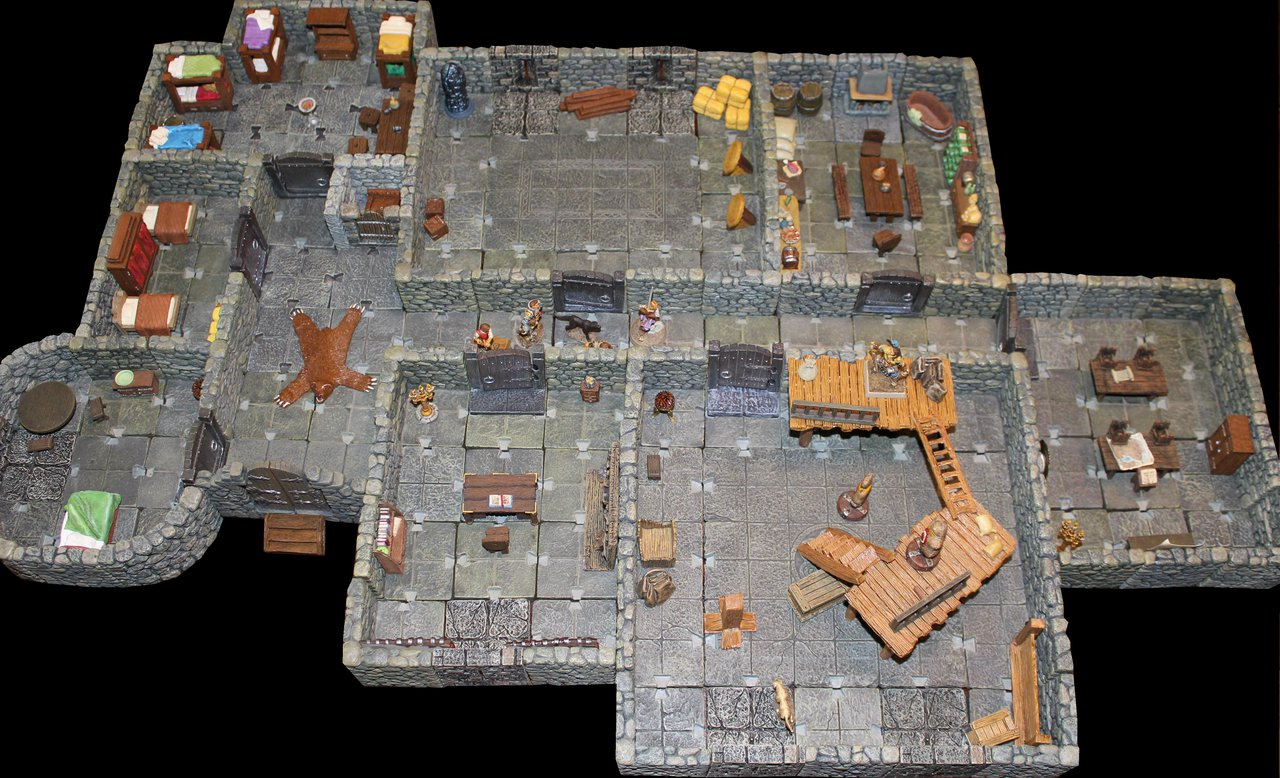
\includegraphics[width=0.39\textwidth]{images/Endrin-military-academy-550435227.jpg}
	\caption{Endrin military academy}
	\label{fig:Endrin-military-academy-550435227}
\end{figure}

\begin{figure}[h]
	\centering
	\includegraphics[width=0.39\textwidth]{images/Ambush-in-the-training-room-550436061.jpg}
	\caption{Ambush in the training room}
	\label{fig:Ambush-in-the-training-room-550436061}
\end{figure}

"We come in peace ... Janros Rainwater, I presume. We're not here to steal from you, we're here to talk. We want to ask you about Yuuna", the bard says.\\

"Yuuna, do you know where she is?" he jumps to Quint's words.\\

"We were actually hoping you might tell us", Quint continues with a slight tone of disappointment.\\

"She's been missing for a couple of days now, she hasn't been at work and she's not at home."\\

"So you've been to her place. Maybe you're the one who got in through the back window", Sjo speculates.\\

"Indeed I was. The only thing I found was a wooden toy house, representing a local little restaurant. I don't know if you're familiar with it, 'The Traveling Man' it's called. I went there and asked about her, but I didn't find anything."\\

"So, you're here all by yourself, or what?" Balian notices.\\

"Just me and Boomer", Janros pets the dog. "Everyone else was called back into service, when all the trouble started after King Eodred died. I am one of the seniors here, so I stayed behind to keep an eye on things. There have been a couple of attempts at looting since the quarantine. That is why I attacked you ... I do apologize, of course."\\

"Don't worry about it, hard times demand even harder measures. We understand," Quint assures the man." Still, I imagine you do not know what is happening to your brethren on the mainland. They are much worse off."\\

"My brothers, what do you mean?"\\

"Well, there is no easy way to break this news to you," Sjo explains. "The Sable Company has been outlawed after Commander Endrin attempted to murder the queen."\\

"He did what?"\\

"He tried to kill her, shot an arrow straight into her head, he did", Balian goes on. "Should have killed her on the spot, but she pulled it out like it was a splinter and planted it right between Endrin's eyes. Game over for him, and his troops with him. The Gray Maidens have been all over town hunting the Sable Company down."\\

"By the gods, I must get over there and help them!" Janros shouts.\\

"If some of your colleagues are still alive and at large, they've probably gone into hiding already. There's not much you can do", Quint says.\\

"The hell there isn't. I cannot sit idle while my friends are being butchered or arrested. I have to help, or at least I have to try!" Janros objects.\\

"Why don't you come with us to find Yuuna?" Sjo suggests.\\

"As much as I love her, duty calls. I'll give you the wooden house, though I don't see what good it will do. Then I have to go."\\

The toy house does not only portray 'The Travelling Man', but also the square in front of it, which is famous for its occasional otyugh outbursts. A small wooden circle represents the plug over the sewer entrance. Puk notices he can remove it and sees a strange, vaguely heart shaped indentation underneath it. Studying it, Quint realizes that it perfectly fits the feet of the wooden Yuuna figurine. So she is not in 'The Travelling Man' after all, but in the nearby sewers!\\

The companions quickly say goodbye to Janros Rainwater and Amin Jalento, who has agreed to watch over the Endrin academy in Janros's absence. Afterwards they hurry to the square in front of 'The Travelling Man'. A heavy grid covers a substantial hole in the ground, which is normally winched open every Oathday to feed the garbage eaters. Next to this giant plug is a smaller manhole with a lid, which opens easily, revealing a ladder down. A scared female voice rings from below: "Is anyone there? Please help me!" The slightly exotic accent betrays her Vudran heritage. It is Yuuna! And she is still alive!\\

The adventurers climb down and\hyperref[fig:Otyugh-sewer-pit-Korvosa-550449437]{ find a stone set of stairs leading further into the dark } . Below a light shines from a locked cage which houses a scared woman. She clings to the bars in the front, trying to avoid the tentacles swinging at her in the back of the cage. A hungry otyugh is barred from entering at the other end, but it is attempting to grab the Vudran with its long feelers through the iron ribs. \\

\begin{figure}[h]
	\centering
	\includegraphics[width=0.39\textwidth]{images/Otyugh-sewer-pit-Korvosa-550449437.jpg}
	\caption{Otyugh sewer pit Korvosa}
	\label{fig:Otyugh-sewer-pit-Korvosa-550449437}
\end{figure}

Then a second female voice calls out: "Once again we bear witness to your slow and feeble attempts at rescuing those you love! You should have been here hours ago! Still, I'll give you this one shot at saving the damsel in distress to kick off our little game. There will be no such mercy from here on, though. So, prove to me how fast you are at rescuing your friends or watch them die! No time to dally." With the sound of metal grinding on stone several portcullises rise and at the same time the door in the back of Yuuna's cage swings open, clearing the way for the otyugh to charge in.\\

"Puk, use the {\itshape cloak of the pixie king} !" Quint shouts as everyone gathers around the halfling who zaps the party into the cage. Arriving behind the bars gives the companions the opportunity to confront Yuuna's foe, but it also keeps them safe from the pair of otyughs that enter the central room through the other opened passages, or at least the heroes think so, because the creatures simply stretch their appendices through the iron poles to attack. Balian cuts a deep slash into the sewer monster in the cage, but then he sees an extraordinarily large specimen emerging from one of the lower pipes. \hyperref[fig:Otyugh-attack-in-Old-Korvosa-550450012]{ The creature glides its mighty tentacle through the bars and grabs the ranger with it } , pulling him against the iron and crushing his ribs. Quint tries to save his friend by nauseating the huge grappler with  {\itshape cacophonous call} , but his magic is easily resisted. One of the normal sized beasts also grabs Balian through the metal, putting the ranger in dire straits. Inside the cage the otyugh bites Sjo with its filthy teeth, but it doesn't survive Puk's deadly gashes. Next Sjo draws upon his mastery over the element of fire and hurls a  {\itshape fireball} at the three monsters in the central room. Burned sewage is not exactly a pleasant smell, but the crisp meat on the otyughs' backs is definitely a welcome sight. Balian fails to free himself from the huge tentacle and has to resort to his dagger to gash the tendril that squeezes him. It takes several rounds of cutting and two extra  {\itshape fireballs} to drop another otyugh and send the two remaining ones running. \\

\begin{figure}[h]
	\centering
	\includegraphics[width=0.39\textwidth]{images/Otyugh-attack-in-Old-Korvosa-550450012.jpg}
	\caption{Otyugh attack in Old Korvosa}
	\label{fig:Otyugh-attack-in-Old-Korvosa-550450012}
\end{figure}

While Yuuna thanks Quint profusely for saving her, Balian notices another toy house in the corner. This one resembles the temple of Aroden, an old crumbling church, devoted to the worship of the city's former most popular god, until he disappeared a century ago. A pitiful trio of clerics is rumored to maintain the building as best they can, going so far as to hold services every Sunday for a handful of patrons, most of whom are not worshippers, but simply curious observers. The feet of the Korwick doll fit into an indentation inside the wooden miniature building.\\



	%!TEX root = ../crimson_throne_book_main.tex
% 2015-08-22
While making their way to the temple of Aroden, the companions find the streets mostly abandoned. Has the plague decimated this district so thoroughly that there is hardly anyone left or are people so scared of the emperor that they dread coming outside? The first reason will surely have a huge impact, but fear of Pilts Swastel definitely plays a part as well, which becomes clear by the little game some ragged children are playing. Faking an execution with some simple wooden stick dolls and guillotine, the kids sing a macabre song:\\

"Off with your head, off with your head!   Sjo tries to scare away the children by telling them he will grow two heads if his is ever chopped off, but these little upstarts are not spooked easily. Having survived as long as they have in these inhuman circumstances has clearly hardened them. They simply change their lyrics to "off with your heads The temple of Aroden is an old, crumbling building which has lost almost all of its former splendor. Sjo uses a new neat trick and summons a pair of fiery wings, allowing him to fly up to the bell tower. Using his mace, he strikes the brass bell in an effort to distract whoever is inside the building, while his friends burst through the front doors. The ring of the bell is answered by the rattling of chains and the wails of a young child crying out in pain. When Balian pushes open the front doors, he finds the temple covered in a web of chains. A strange figure, dressed in tattered robes, is standing at the other end of the room. Multiple chains flow from his body and seem to bring the entire iron meshwork to life. Above the altar hangs the squirming form of Korwick. The shackles are squeezing him ever tighter and make him scream out in agony. Balian and Quint find a path through the tangled web and close in on the enemy, who unleashes a cacophony of dark, soul-shaking howls from the pits of hell. A pitch-black cloud spreads out around him and the overwhelming scream deafens the two brave heroes, who summon the strength of their will to fight back an even nastier effect. Puk and Sjo enter as well, but the Shoanti is the only one who can see in the dark - his limited {\itshape clouded vision} does have its advantages after all. He notices that the evil fiend moves through the sea of iron braids with ease, while his friends all get caught in it. The healer throws a  {\itshape burning hands} on the creature, but the flames simply glide off its body, leaving it unharmed. Spyder's keen sense of smell allows the dog to locate the devilish monster in the darkness and attack it with a  {\itshape critical} bite. But the canine's teeth do almost no damage. So the devil needs specific weapons to be hurt; unfortunately no one in the party possesses the knowledge to know which. Groping around in the blackness and struggling with the entangling chains makes the party very inefficient. Balian manages to pull free from the grasp of the web and makes his way to the monster, but as the darkness drops away, he now faces the  {\itshape unnerving gaze} of the sacristan kyton - who has lowered his hood - and is staggered. The chain devil keeps moving agilely through the crisscross of strings and lashes out mercilessly with his own spiked chain, making all the heroes bleed. Quint stumbles out of the church and pull out his wand of  {\itshape feather step} to allow himself faster movement in this difficult terrain. \hyperref[fig:Chain-devil-in-the-temple-of-Aroden-555419466]{ The combination of the entangling chains and the unsettling eyes of the kyton make this fight very hard. } The companions keep getting stuck in the iron web - even the dexterous rogue Puk - and the monster's gaze continually steals actions from the heroes if they fail to summon the willpower to resist. The only upside is that the devil's most efficient tactic is to cleave away at his enemies, thus spreading the damage over multiple targets, instead of focus firing. Of course, this forces the companions into combat healing as well, Puk has to pull out a potion to stay in the fight, while Quint resorts to his  {\itshape wand of cure serious wounds} and Sjo burns through his own healing magic. Quint makes it to the altar, where the strangling chains have forced poor Korwick into unconsciousness. He saves the boy's life with a touch of the wand. Meanwhile Balian scores his first hit; his greatsword's magic is not empowered to bypass the devil's damage reduction, but his heavy hit still deals a fair gash. The ranger's skill of following up when his enemy tries to step away also proves its worth, forcing the devil to stop moving about. Sjo also closes in on the kyton and strikes hard twice. It takes many more rounds of healing, striking and trying to avoid the creature's gaze or facing the potential staggering effect before Puk finally gets into position and finds that the silver of his off-hand short sword actually does full damage to the fiend. The halfling's first strike is also his last, as the sacristan kyton finally drops to the floor, defeated at last. \\

\begin{figure}[h]
	\centering
	\includegraphics[width=0.4\textwidth]{images/Chain-devil-in-the-temple-of-Aroden-555419466_mod.jpg}
	\caption{Chain devil in the temple of Aroden}
	\label{fig:Chain-devil-in-the-temple-of-Aroden-555419466}
\end{figure}

The companions dig deeply into their resources of healing wands to restore everyone to full health. Korwick has lost consciousness again, but is still alive! Puk finds another wooden miniature building, representing the Copper-Beater hall, an enterprise close to the pier of Eel's End. This wooden toy house fits the feet of the Heldrin puppet. Sjo also discovers the bodies of the three priests of Aroden in a backroom of the temple. They have all been slashed to death by the kyton's cruel barbs.\\



	%!TEX root = ../crimson_throne_book_main.tex
% 2015-08-22
Travelling to the Copper-Beater hall sends the party through the heart of the emperor's district again. They pass four of Pilts' ruffians on the way, who glare at the heroes and start chuckling, but do not engage. As the thugs walk down the street, a gaunt man with a blank stare in his eyes exits from an alleyway. He's clinging a simple wood-chopping axe in his grasp and is dressed in an ill-fitting and awkwardly strapped leather armor. The man pays the companions no heed, but trots off after the four bullies instead. Quint shouts out to him, but his cry only makes the emperor's men look back and notice the haggard man approaching. The wretch raises his axe and charges the thugs, but his inept swing goes wide and the next moment he is on the ground with the four ruffians on top of him. They cheerfully disarm the poor man and drag him along.\\

\hyperref[fig:Copper-beater-hall-Korvosa-555420262]{ The Copper-Beater Hall is an impressive structure } with a fancy front door. Peeking through the windows Puk makes out a luxurious meeting room and a richly decorated office, which are both deserted. The side of the building sports large warehouse doors through which crates and containers are normally transported in and out of the building, but they are shut now. The three chimneys are spouting black smoke, but there is no thunder of pounding hammers, which usually resounds from within. There is a third way in on the backside of the factory, which looks like the entrance for the workers. This is the entry point the companions choose. \\

\begin{figure}[h]
	\centering
	\includegraphics[width=0.4\textwidth]{images/Copper-beater-hall-Korvosa-555420262_mod.jpg}
	\caption{Copper-beater hall Korvosa}
	\label{fig:Copper-beater-hall-Korvosa-555420262}
\end{figure}

The heroes walk into a small changing room with some clothes and leather aprons hanging from pegs on the far wall. The dry, mouldy bread on the table suggests that the workers have not been here for some time. The door leading to the copper-beating furnaces feels slightly warm to the touch and Puk's observant ears pick up some low growls on the other side. Sjo casts {\itshape resist fire} on Balian and Puk, trusting that his innate fire resistance and Quint's ring will prove enough protection to withstand any potential fire attacks. As Balian pulls open the door, he is met by three powerfully built wolves, the size of draft horses, with ebony fur and fiery eyes. Spikes protrude from the fur on their backs which seems to flicker with red flames. The biggest of these hellhounds turns towards the intruders and spews forth a sea of flames, engulfing all companions in an inferno. His breath weapon also lights up oil which flows through several gutters in the workplace. Tied up in front of the blazing furnaces is Heldrin, who is now struggling to avoid the wall of fire that spreads through the room. Puk can evade the fire breath completely, while Quint and Balian get seared moderately. It is the fire-loving Shoanti, however, who takes a heavy burn. Before he can recover, Sjo gets jumped by a second warhound, whose fierce bite puts him down. Quint pulls Spyder, who is also heavily charred, behind the open door and waits for Puk and Balian to lure the hellish canine into the changing room. Then he kicks the door shut, giving his friends the opportunity to quickly take out this opponent. Meanwhile the bard uses his wand to put Sjo back on his feet. \hyperref[fig:Facing-Nessian-Warhounds-in-Copper-Beater-Hall-555420948]{ Next Quint reopens the door and Balian charges the two remaining Nessian warhounds the workplace } . Through sheer luck Heldrin has avoided most of the flames and is still on his feet, though barely. Fortunately the oil in the gutters has burned away and the fire in the room is now dying out. Balian cleaves and Quint makes it to his side, for the ranger is taking multiple bites and is in desperate need of healing. Puk tumbles into an advantageous position and works his sneaking magic. Sjo aids in healing Balian, whose heavy hits kill off a second hound, but the ranger still gets dropped himself before his friend finish off the last Nessian warhound. \\

\begin{figure}[h]
	\centering
	\includegraphics[width=0.4\textwidth]{images/Facing-Nessian-Warhounds-in-Copper-Beater-Hall-555420948_mod.jpg}
	\caption{Facing Nessian Warhounds in Copper-Beater Hall}
	\label{fig:Facing-Nessian-Warhounds-in-Copper-Beater-Hall-555420948}
\end{figure}

The healing wands are drained further of their {\itshape cures} and the companions realize they are slowly getting through their resources with at least one more rescue attempt ahead. Quint notices a wooden replica of the Old City Hall, the tall spire of which has in indentation which fits the feet of the Mouse miniature. At one time in history, this belfry-like structure was the tallest building in all of Varisia, until the Arvensoar in Magnimar stole away that distinction for more than a decade. Korvosa quickly reclaimed the honor with the completion of the north tower on Castle Korvosa, though. The Old City Hall's black stone walls have led to people calling it the Charcoal Palace. It served Korvosa as city hall for 60 years, until Remsev Ornelos decided that its many stairs leading up the tall tower were a terrible inconvenience to anyone working there. The building might have been prestigious in design, it was also very impractical. So when the city expanded to the mainland, the Korvosans constructed a new, more practical city hall in North Point, which remains in place until today. The Old City Hall has housed a handful of private initiatives over the last two centuries, but it has stood empty for at least as long as any of the companions can remember, serving mainly as a landmark in the oldest part of the city. Will this tall tower be the arena for the party's confrontation with Alika and Rolth? Judging by their resources, the heroes certainly hope so. 

	%!TEX root = ../crimson_throne_book_main.tex
% 2015-09-12
With Heldrin and Korwick safe, two of the three children living with the party in the villa are now out of harm's way. Heldrin joins his friend in the Endrin Academy while the companions head over to the old city hall to rescue the third and last missing lamb: Mouse. Korvosa's former townhall is situated in the quieter part of the island, up on Garrison Hill, quite close to the Palace of the Arkona family. Apparently the nobleman's name still carries enough weight to keep the emperor's men at bay. The high tower of the abandoned building is impressive. The companions figure they will have to climb it to the top floor, with the stories in between forming the perfect set-up for traps. Proceeding with caution the party locates and dismantles three traps on the lower floors.\hyperref[fig:Korvosa-Old-City-Hall-559764706]{ Climbing the tower turns out to be safe } , at least until the companions reach a very high-ceilinged room in which the stairs wind up to the top floor. About halfway up the stairs acid rain starts pouring down on the heroes, burning their flesh. Balian scurries all the way up to shut off the sprinkling system. One wooden trap door separates the party from their destination, but Puk and Balian find powerful magic protecting the lid. Quint sacrifices himself and suffers the effects of a  {\itshape symbol of pain} to open the trap door, while his friends hide on the floor underneath to keep out of the harmful magical blast. Next they storm through the hole, with Balian and Puk leading the way. \\

\begin{figure}[h]
	\centering
	\includegraphics[width=0.4\textwidth]{images/Korvosa-Old-City-Hall-559764706_mod.jpg}
	\caption{Korvosa Old City Hall}
	\label{fig:Korvosa-Old-City-Hall-559764706}
\end{figure}

The top room has windows on all sides, overlooking the region. There used to be a huge clock in here, but it was removed and melted down decades ago, when queen Domina needed funds to finance her ever growing hunger for fancy building projects. A balcony juts from the south side of the tower; the open door reveals Rolth standing in the wind. Tied up, on the other end of the railing, is Mouse. One nudge would suffice to push him down.\hyperref[fig:Final-showdown-with-Rolth-and-Alika-559765837]{ Barring the way to the door are three bearded devils and Alika. } Hate flickers in her eyes as her brother steps into view. "For the glory of Urgathoa! Time to settle the score!" she hisses as she removes a long leather glove from her right hand. Her limb is completely stripped of flesh, leaving nothing but bone, like an undead graft on living tissue. \\

\begin{figure}[h]
	\centering
	\includegraphics[width=0.4\textwidth]{images/Final-showdown-with-Rolth-and-Alika-559765837_mod.jpg}
	\caption{Final showdown with Rolth and Alika}
	\label{fig:Final-showdown-with-Rolth-and-Alika-559765837}
\end{figure}

Sjo quickly gauges the situation and notices the schmuck smile on Rolth's ugly face, indicating that the necromancer feels in control with the little hostage at his mercy. The Shoanti summons his fiery wings and flies out, surprising the evil wizard and positioning himself between the foul man and his prey. Rolth looks most displeased and lifts off into the air himself ... he obviously prepared a {\itshape fly} spell. Still, he is frustrated, having hoped to threaten the party with the helpless boy and cast spells at them from a safe position. He calls into being a  {\itshape wall of force} that block the doorway and curses Sjo for ruining his plans once again. Sjo pulls Mouse over to the safe side of the railing and lifts off. The two flying men engage in an aerial dance, swirling around each other, trying to hurt one another with magic. Sjo easily withstands the burns of two scorching rays and scoffs at Rolth's attempt to  {\itshape fear} him, but he sees his own  {\itshape hold person} and  {\itshape dispel magic} fail as well. Meanwhile Puk and Spyder are keeping the bearded devils occupied. One of the creatures claws into the halfling and rends his flesh with his filthy beard, while the other two wield glaives and cut Balian and his pet dog from a ten feet distance. Alika immediately charges her brother and starts hacking away at him. The ranger returns the favor by showing no mercy when he wields his greatsword. Doubt still creeps through his veins as he misses his target more than he hits it. Quint pulls out the {\itshape wand of cure serious wounds} and reverts to healing again. He also launches a discouraging  {\itshape satire} in infernal, weakening the devils' attacks. Puk has already taken considerable damage, but strengthened by Quint's cure, he survives long enough to cut down a bearded devil. Next thing he knows is darkness, as the glaive of another devil drops him as well. Alika's skeletal claw hit several times, but deprived of an opportunity to sneak, the rogue does limited damage. When Balian's strokes hit, they are much more harmful. Even when the ranger realizes his sister is close to death, he does not hold back. He drives his blade through his sibling's chest, finishing her off once and for all. The foul necromancer corrupted her beyond saving, Balian sadly realizes. Death was the only release from this mortal existence that was left to her. And since she was Balian's responsibility, the cruel task fell on him. Still, the time to mourn will have to wait, for there are two dangerous devils left. Quint revives Puk and joins him in cornering one of the opponents, leaving the other one for Balian and Spyder. The heroes now have the upper hand and finish the job in a few rounds. Outside the flying struggle continues. Rolth blasts Sjo with a powerful {\itshape lightning bolt} , but the Shoanti casts some healing magic and flings himself at the wizard, grappling him. Rolth curses even more in frustration and barely succeeds at mumbling the words of  {\itshape dimension door} . From one second to the other he disappears. Sjo figures out that the wizard has to flee to a place close-by that he is familiar with, like somewhere else in the tower. The Shoanti flies down to the front door, quaffing more healing potions on the way. He enters the front hall again and stumbles upon his opponent in there. He jumps the necromancer once more and grabs him in a choking hold. This time Rolth fails his effort to cast magic and fizzles his get-away  {\itshape teleport} spell. Sjo is determined not to let go of his prey and clasps his arm tightly around the man's throat, sending fire through his hands again and again. He only stops when he has no more fire left. Rolth's charred and lifeless body tumbles to the ground. The companions recover some loot and find a special document in Rolth's possessions. After surviving the explosive runes on the parchment, Quint discovers it holds the precise wording of an infernal contract between Rolth and a devil named Chyvvom, promising the necromancer the services of infernal creatures up to five times in return for his immortal soul. The companions do not regret having had to fight their way through the servants from hell, as they now realize that Rolth will pay the price for these creatures' assistance with eternal torture in the afterlife. A fitting fate for one so foul!\\



	%!TEX root = ../crimson_throne_book_main.tex
% 2015-09-13
 \section{[Edit]}



	%!TEX root = ../crimson_throne_book_main.tex
% 2015-09-13
Sjo's player wrote down his version of the end of the session:\\

The Necromancer just escaped with a dimension door and Sjo - driven by the momentum of his charging attack- lands on the balcony where Mouse is still lying gagged. The healer suppresses his urge to go to the kid to undo his bindings but instead spies the sky in search of Rolth. Where did that filthy piece of s!~% go? Acting on his instincts Sjo jumps off the balcony and summons his fiery wings to glide down, back to the basement of the belfry tower. Getting more and more confident with his new form of movement the Shoanti takes his time to flutter down while quaffing 2 healing potions before his feet touch the ground.\\

Sjo pushes the doors of the building for the second time and is surprised to see Rolth standing in the big entrance hall. "You filthy piece of Shoanti-s~#$" the Necromancer shouts. "Why you just don't die as everybody else?" and 5 missiles shoot from his fingertips targeting the Oracle. Sjo starts to charge towards the necromancer, stoically taking in the missiles without giving a glimpse. Luckily the Shoanti was almost completely healed using his remnant potions.\\

In a final leap Sjo throws his full weight at Rolth and both crash to the ground. The necromancer tries again to escape the clutches of the furious Shoanti by casting a spell which would take him farther away from his nemesis. But this time he is not so lucky and the spell fizzles before it takes effect. Sjo seizes the opportunity to slip his arm around the filthy death-reeking man's neck and starts to strangle him. In his rage he calls out to the domain of Asmodeus to get that all-consuming fire. By setting his own arms ablaze and ever squeezing harder, Rolth only has a couple of feeble attempts left before all the life fades away from his body. While the necromancers' consciousness slips away, Sjo whispers in the dying mans ear: "I sentence you to die Rolth and hope you'll burn in hell for all what you did to us and the kids ..."\\

Even when the body goes limp, Sjo keeps getting on to that burning fire until he's exhausted.\\

---\\

Asmodeus is sitting in audience, listening bored and half-heartedly to the umpteenth dispute about some contract. Suddenly the Prince of Darkness' attention is caught by a little disturbance in one of his domains. Something is pulling fire with that much hate and force that it gets to his attention.\\

Shifting his attention away from this ever-dull audience the Ruler of Hell notices that the power is drawn by some Shoanti warrior in an amusing attempt to fry someone's head.\\

There's something about these two that gets the Dark Lords attention: This Shoanti must be that runaway pupil Reebs keep ranting about in his communes, and the other one... yes, that's the necromancer who - not even a day ago- haggled endlessly about a contract he wanted to sign.\\

The Lord of the Pit is amused with the situation: this filthy worm will fulfill his end of the contract very soon it seems. And the bigger irony is that this Shoanti-runaway is now fulfilling a service to him without even having a clue.\\

Burning his head every day for at least a hundred years seems like a good start to teach this would-be necromancer a little lesson in humbleness. As for this Shoanti-character: might be worth keeping an eye on that one.\\

The Prince of Darkness stand up from his throne - dismissing the audience- with his thoughts full of crispy heads ...\\



	%!TEX root = ../crimson_throne_book_main.tex
% 2015-09-26
The companions return to Vencarlo's burned down academy and build a pyre for Alika. Sjo prays to Pharasma to show mercy on the poor, misguided girl's soul and Quint pours his sorrow in a sad song. Balian just watches in silence as his sister's remains are consumed by the flames, hoping that she will find some kind of peace in the afterlife. Afterwards the party heads to the Endrin Academy, where Amin Jalento, Korwick and Heldrin are still safe. The sadness of Alika's demise is somewhat compensated by the joy of Mouse, reconnecting with his two best friends. Realising that they accomplished nearly the impossible by saving the three boys from the clutches of death definitely brings some comfort. Weary of today's trials, our heroes quickly slink away in sleep's embrace.\\

\section{22 Erastus 4708}

The next morning immediately proves how resilient young boys can be. Although they went through a traumatizing experience, Korwick, Mouse and Heldrin do not appear dazed. Sjo feels proud when he sees that his wards put food first in their priorities, plundering the provision cabinet for salami. Having faced the revenge of a deranged necromancer did not break little Mouse, as he recounts to his friends how the heroes saved him from the bad man with much gusto. Who knows, these boys might have the making of heroes in their hearts as well.\\

Following up on Amin Jalento's hint that Salvator Scream, the painter, visited his master Vencarlo Orisini on several occasions,\hyperref[fig:Where-is-Salvator-Scream-562539967]{ the companions head over to the artist's house } . The decripit building on the Narrows of Saint Alika appears in an even sadder state than the last time the party came here. As Balian moves in to pry open the lock on the front door, he notices that someone beat him to the punch. It looks like Salvator Scream already had 'visitors' a couple of days ago. The door swings open to reveal a front room with multiple muddy tracks covering the floorboards. The footprints lead to the bedroom with a single bed. The blankets and pillow atop are in disarray and there is no sign of the painter. \\

\begin{figure}[h]
	\centering
	\includegraphics[width=0.4\textwidth]{images/Where-is-Salvator-Scream-562539967_mod.jpg}
	\caption{Where is Salvator Scream?}
	\label{fig:Where-is-Salvator-Scream-562539967}
\end{figure}

Salvator's studio stinks of must and mildew. At one time this room was a sanctuary where an inspired madman committed the visions of violence and horror in his head to canvas, but Salvator's latest work shows none of that brilliance.\hyperref[fig:Salvator-Scream-studio-562540993]{ Frustration must have taken hold of the artist, as he destroyed his own lackluster creations. }  \\

\begin{figure}[h]
	\centering
	\includegraphics[width=0.4\textwidth]{images/Salvator-Scream-studio-562540993_mod.jpg}
	\caption{Salvator Scream studio}
	\label{fig:Salvator-Scream-studio-562540993}
\end{figure}

Outside the party comes across some of the emperor's men. Quint inquires about Salvator Scream's whereabouts and easily tricks the goons into admitting that mister Scream is a 'guest' at their master's. Seeing this as an easy opportunity to make some money, Corl, one of the thugs, offers to procure an audience with the emperor in exchange for a pay-off. He wants 25 gold sails, but is haggled down to a mere 5 gold pieces before he takes to companions to the emperor's poor excuse of a palace.\\

Emperor Pilts Swastel heartily welcomes the heroes back to his place and after graciously accepting their gift of a magic cloak as a tribute, he agrees to let them speak to the painter for a couple of minutes. He takes the companions into\hyperref[fig:Pilts-Swastel-emperor-of-Old-Korvosa-562541723]{ the building behind his throne } and leads them to a dark, unpleasant room, scarcely more than a cell, in which Salvator Scream is pining away. Pilts has no intention of leaving the party alone with the painter and sits down in a chair as he invites his guests to have their little conversation. The emperor feels comfortalbe in the company of his four personal bodyguards, who easily kicked the heroes' butts last time. \\

\begin{figure}[h]
	\centering
	\includegraphics[width=0.4\textwidth]{images/Pilts-Swastel-emperor-of-Old-Korvosa-562541723_mod.jpg}
	\caption{Pilts Swastel, emperor of Old Korvosa}
	\label{fig:Pilts-Swastel-emperor-of-Old-Korvosa-562541723}
\end{figure}

Scream looks in bad shape and seems ill at ease with the emperor staring down his face. Still, the companions convince him to talk. His tale starts with Neolandus Kalepopolis, the seneschal of Castle Korvosa. The two of them became friends a few years ago and regularly shared drinks to discuss art, religion and history. Then, three months ago, things started going horribly wrong. First Scream lost his muze and and three weeks later Neolandus Kalepopolis showed up on his doorstep, on the morning of King Eodred's death. The seneschal was grievously wounded and had lethal poison running through his veins. Kalepopolis drifted between life and death for many weeks, but somehow the good man survived, taking even longer to fully recover. When he finally felt better, Neolandus entrusted Salvator Scream with the terrible truth of what had happened to him. He had discovered that Queen Ileosa was responsible for killing her husband and that she had enlisted the aid of the Red Mantis, a secret organisation of deadly assassins. Two of those dreaded killers in their red insectoid armor had tried to slay him, but Neolandus escaped, barely alive, fleeing to Old Korvosa.\\

Neolandus admitted that he had never been a fan of Ileosa, but in the final weeks of Eodred's life, she had somehow changed for the worse, whatever that entailed. The seneschal did not share more on this topic with Scream, claiming "the less the painter knew, the safer he'd be". Neolandus also realized that he the painter's humble shack was no safe place to hide any longer, so now that he finally felt better, he wanted to find another refuge. Scream suggested the Arkona's, Old Korvosa's only remaining noble family. Since the island had already been cut off from the mainland at this point, the Arkona's seemed like the safest place to stay. The seneschal had his doubts, but Scream convinced him there was no alternative. Moreover, the artist liked Glorio Arkona, to whom he had sold several of his paintings in the past. He took Neolandus Kalepopolis there and hasn't heard from him since. The Arkona's seemed nice enough when he delivered the seneschal to them and Salvator Scream had felt like he could trust the nobles.\\

That changed after Scream talked to Vencarlo Orisini. The fencing master never tried to hide his disdain for House Arkona and seemed convinced that the family was involved in all kinds of dark, criminal activities. He was so outspoken about his distrust for these nobles that it took Scream three visits, spread out over more than a week, to gather the courage to tell him that he had delivered Neolandus Kalepopolis into their hands. Orisini got raving mad when he heard that, claiming that the seneschal would have been better off in Ileosa's dungeons.\\

When the heroes inform Salvator Scream that Vencarlo was attacked by the Red Mantis and has disappeared after escaping the assassins, the painter gets even more worried. He has no idea where the fencing master could be, but if he's still on the island, he might very well have gone to the Arkona Palace to find the seneschal.\\

At this point Pilts Swastel interrupts the conversation. The content smile on his face shows that he is pleased with what he has just overheard, but now he claims that time is up - the cloak the heroes gave him only bought them so much time. Sjo shoots a glance of understanding at Quint and the bards spurts into action, suddenly casting a {\itshape haste} spell. Balian takes advantage of his accelerated actions to chop down one of the emperor's bodyguards with three heavy blows. Puk throws himself at Pilts Swastel and almost takes the man out with three vicious lashes. Spyder finishes the job by grabbing the surprised emperor by the throat and choking the life out of him. The remaining bodyguards back down when Sjo steps in front of them, growling like a mad dog. The fight ends as quickly as it began, just like the first confrontation with the emperor, only this time the companions are on the winning side. The emperor's rule is over! Sjo drags his dead body outside and throws it on the guillotine. Most of the emperor's men have already cleared the scene; some of them are glancing at the adventurers from a safe distance and witness how their precious leader loses his head under his own  {\itshape tall knife} . Sjo shouts out a challenge to them: "The emperor is dead! If I ever catch as much as the smell of you cowards, you'll suffer the same fate! Now RUN!" At that the mob disappears, leaving only a stupefied one-eyed gnome on the open-air balcony. When Sjo leans over him, the mute creature starts gesturing that he is innocent, pointing at the emperor's remains as the source of all evil. With a nod Sjo lets him go and the gnome jumps at the chance to get away. Quint comes out with his hand on Scream's shoulder. "You're free to go, Salvator, Swastel won't bother you again."\\

"So, what do we know about this Arkona dude?" Balian inquires. "We met him once, at the great council in the castle ...  He seemed pretty level-headed to me. And didn't we see his sister at the celebration in the Jeggare Museum, before the opera?"\\

"Yes, we did", Quint confirms. "I've picked up many rumors over the years. They say that the Arkona's are one of the richest families in Korvosa - if not the richest. Their home is supposed to be a magnificent marble castle, up on Garrison Hill. They do business with the distant nation of Vudra ... very lucrative, since they are one of the few trading companies allowed to import and export goods there. Most of their vessels never even make it to Korvosa, preferring to sell their cargo in the Inner Sea region instead.\\

The guards at their palace are Vudran too, as is Glorio's other half. Most people think he has a wife and two kids in Cheliax, but I've heard his spouse is a Vudran beauty who has never left her home country. She's raising his son and daughter there as well.\\

It was actually one of Glorio's forefathers who established the profitable relations with Vudra, a man named Nerio Arkona. He saved his house by pouring his last coins in a trading vessel, the {\itshape Reprieve} it was called ... hmm, must have been two and a half centuries ago, I reckon. Anyway, his journey was fraught with peril, but he survived and turned his enterprise into a smashing success. Upon his return, three years after he had left, he ordered the Arkona Palace built. Yes, he really managed to turn his fortune around, going from nearly bankrupt to filthy rich." "Still, why does Vencarlo think he is so dangerous?" Puk wonders. "Aren't the Arkona's known for their generosity, providing cheap housing for the poor and sometimes even handing out money in the streets?"\\

"They are", Quint nods. "The man is quite popular and respected in this district. But this image of the big-hearted benefactor hides a less admirable truth. I'm afraid Vencarlo may be right. I've also heard that the Arkona's are heavily involved in crime, through the Cerulean Society, to be exact. Korvosa's thieves' guild does some dirty business, but by never crossing the line and by paying a hefty vice tax, they can get away with it ... even with being a 'guild' in a city that allows none. What's their leader's name again? Boule! A brute of a man, if rumors be true."\\

"Doesn't really matter how good or bad our man is, I suppose", Sjo interjects. "We'll find out soon enough as I suggest we pay him a visit. What do you say?"\\

"I guess we must", Balian smiles. "Let's knock on his door for a cup of tea."\\

"Coffee", Quint remarks. "Vudrans drink a bitter black tea they call coffee."\\



	%!TEX root = ../crimson_throne_book_main.tex
% 2015-10-03
While making their way to Palace Arkona, the companions worry about how to get inside. They have met Glorio Arkona once, but that might not be enough to broker an audience with the man. Upon approaching the compound our young heroes are marveled by its beauty. Black marble walls, topped with swirly iron decoration, line the grounds. An intricately forged gate allows a peek inside, revealing a magnificent marble palace with gold pillars, high windows and elegant minarets. The large, open garden hosts stylized bushes trimmed to look like elephants, opulent patches of imported trees and exotic flowers and fountains and statues depicting strange animals like tigers, apes, snakes and peacocks. Two guards stand inside the gate, but the companions' attention is immediately drawn to a third person walking up from the palace with a graceful stride. It is Selena, the Vudran beauty who was manipulating the uprisings in the city prior to the plague and who orchestrated the failed murder attempt on Aisha Leroung during the {\itshape Passion of Saint Alika} opera. She was also the one who alerted Balian to the threat at the Carowyn party, which allowed our heroes to take out the shadow creature before it killed off half of the city's noble youngsters. "At last you have arrived. My master has been expecting you. Please, follow me", she says as she opens the gate and leads the guests inside. She proceeds them up to the palace and through the front door, which is framed by a black marble arch depicting dozens of elephants standing atop each other.\hyperref[fig:Arkona-palace-in-Old-Korvosa-563928457]{ A rich hallway with a luxurious red carpet leads left and right, providing a pathway between several ebony doors. } Selena walks off to the right and rounds the corner to a corridor leading up to a fourteen-foot tall marble statue of a six-armed woman with four faces on her head, staring in every direction. Sjo is sure she represents a Vudran deity, but his knowledge of that pantheon is too limited to identify her. A door in the middle of the right-hand side of the corridor opens up into \hyperref[fig:Meeting-Glorio-Arkona-563929464]{ a comfortable lounge with a large fireplace and some snug sofas } . Lord Glorio Arkona is standing next to the hearth, with an impressive feline creature lying lazily at his feet. Spyder growls disagreeably as he sees the great tiger. Selena takes up her place between her master and a bare-chested man with broad shoulders, obviously a bodyguard. \\

\begin{figure}[h]
	\centering
	\includegraphics[width=0.4\textwidth]{images/Arkona-palace-in-Old-Korvosa-563928457_mod.jpg}
	\caption{Arkona palace in Old Korvosa}
	\label{fig:Arkona-palace-in-Old-Korvosa-563928457}
\end{figure}

\begin{figure}[h]
	\centering
	\includegraphics[width=0.4\textwidth]{images/Meeting-Glorio-Arkona-563929464_mod.jpg}
	\caption{Meeting Glorio Arkona}
	\label{fig:Meeting-Glorio-Arkona-563929464}
\end{figure}

"Gentlemen," Glorio greets his guests, "it has been a while since last we met. A lot has occured in that time, wouldn't you say so? How are you doing? Can I offer you some refreshments, a glass of wine perhaps? Or would you prefer coffee and chocolate?"\\

While Selena leaves to get the refreshments, Lord Glorio bids his visitors to take a seat. He tells them he has been following their progress closely and appreciates the direction they have chosen recently. Quint immediately asks his host about seneschal Neolandus Kalepopolis and Vencarlo Orisini. Glorio wishes not to discuss them at this time, he states, as he wants to know first where the companions stand with regards to the queen. Lord Arkona makes no secret about having opposed the queen from the very start. He never trusted her, ever since she weaseled her way into king Eodred's bed years ago. Still, he tolerated her as long as the king was alive, but after Eodred's death, her malevolence became increasingly clear. She murdered her husband, got rid of the only person who had the authority to stop her - the senschal - and grabbed power in the city with no regard of its citizens.\\

Sjo objects to this analysis. He remains unconvinced of the queen's guilt, suspecting that she is being manipulated by an unseen power behind the throne. A likely suspect is her new seneschal, Magister Togomor. Lord Glorio smiles at Sjo's suspicions, but wipes them off the table: Togomor did not get involved until after the riots. Before that he was just doing his job in the Acadamae, while Ileosa was already plotting her evil. Sjo also refers to the {\itshape commune} that archbishop Keppira d'Bear of Pharasma performed. Although he agrees that most answers could possibly incriminate Ileosa, there was one question that supported Sjo's theory of a manipulative force behind the queen: the fact that she was being  {\itshape misled} by one of her advisors. Glorio rolls his eyes at this line of reasoning, saying that we are all being misled some way or another. Even the most insignificant effort to mislead Ileosa about the most pointless thing imaginable would have prompted a 'yes' from the commune question. Hardly any proof that the queen is someone else's puppet. Quint also points out that he and his friends met the queen before all the trouble started, when they returned her brooch to her. She was a different woman back then, sweet and innocent, not the ice-queen they saw when she killed commander Marcus Endrin of the Sable Company. Again Glorio nods and says this only supports his theory that the queen is evil and that they have to stop her. Sjo tries to meet his host halfway, by claiming that he does not stand {\itshape against} Ileosa, but  {\itshape for} Korvosa. He does agree that something has to be done about the  {\itshape castle} and Glorio seems to be satisfied with that. Now the Lord of House Arkona is willing to talk about Neolandus Kalepopolis and Vencarlo Orisini. He admits that Salvator Scream, the painter, brought the seneschal to him and that he aided the man by providing a safe place to hide. At Kalepopolis's own request - Glorio claims - he cannot reveal where that is yet. He does know where Vencarlo Orisini is, but fears that it is not in a good place.\\

The swordmaster is a respectable man, Glorio feels, who fights for the right cause as well, albeit mostly on his own, which explains his limited success. Anyway, in his search for the seneschal, Vencarlo Orisini followed up on Scream's hints and came to the Arkona Palace only three nights ago. Apparently the fencing master was a well-informed man as well, Arkona muses, as he knew about the secret dungeons under the palace. Orisini snuck in and did something quite unfortunate: he entered a place called the {\itshape vivified labyrinth} , wrongly suspecting that Kalepopolis would be in there. The labyrinth is some sort of deathtrap dungeon, Glorio sighs. It was constructed over two centuries ago by one of his forefathers, Eduardo Arkona. Glorio points to the painting of a handsome man above the fireplace: his face clearly shows several Vudran features, like a tanned skin and dark eyebrows. A bright red silk shawl covers his hair and completes the exotic look. Eduardo was Nerio Arkona's son, the man who established the trade route with Vudra and erected the family's palace in Korvosa. Eduardo completed his father's work by building the {\itshape vivified labyrinth} underneath, a place said to house  {\itshape Nerio's treasure} . None of the Arkona's, nor any of their Vudran servants have ever entered the labyrinth, as powerful magic keeps anyone with Vudran blood out. Nerio's descendants have repeatedly tried to send hired adventurers in and reclaim the treasure, but no one ever came out of the dreaded dungeon alive. Glorio's grandfather Horatio was the last to attempt such an enterprise, but Glorio's father Marco banned the practice and his son kept to the same rule. This implies that no one entered the vivified labyrinth for two generations, until Vencarlo stupidly decided to go in three nights ago. Glorio has no way of knowing if Vencarlo is still alive, but he wants to offer the companions the opportunity to find out, since Vencarlo is a friend of theirs who is worth saving and the man might make a capable ally in the struggle against the queen ... or castle. Glorio also admits that the 'treasure' intrigues him: it has been an unsolved mystery in his family for over two hundred years and who knows ... it might just be a powerful tool in their quest to help Korvosa. Glorio even offers the heroes a magic ring as payment, hoping the item can be of help inside the labyrinth. Sjo uses Zellara's cards to identity the piece of jewelry as a {\itshape ring of evasion} . 

	%!TEX root = ../crimson_throne_book_main.tex
% 2015-10-03
After a hearty meal Glorio takes his guest into his greenhouse garden,\hyperref[fig:Arkona-palace-garden-with-elephant-statue-563929835]{ which is filled with jungle plants, tropical birds and a refreshing fountain. The most surprising feature in the chamber is a life-sized statue of an elephant, its tusks and trunk raised high. } It takes Sjo a few seconds to realize this animal is not real, but made of stone. Glorio approaches the elephants and presses a hidden button somewhere, making the ground between the statue's giant feet shift aside to reveal a set of stairs. \\

\begin{figure}[h]
	\centering
	\includegraphics[width=0.39\textwidth]{images/Arkona-palace-garden-with-elephant-statue-563929835.jpg}
	\caption{Arkona palace garden with elephant statue}
	\label{fig:Arkona-palace-garden-with-elephant-statue-563929835}
\end{figure}

The companions follow their host down into a vast cavern under the palace. The air is cool, humid and smells of salt. Staring down from the upper ledge, Balian sees a number of rope bridges descending from ledge to ledge until they reach a small quay below. So this is how the Arkona's manage to keep their pantries full, a secret pier inside a sea cave; the perfect place to smuggle goods in or out unseen. The upper rim is overgrown with colored fungi and leads past a solemn tree that moves as our friends approach. Quint notices that Glorio waves his hand, making the tree lean back and stop swaying. Crossing a first rope bridge takes the companions to a ledge with a door in the wall, which Glorio completely ignores. He continues to a second, smaller ledge which has nothing but a natural wall. Sjo spots double doors on the bottom level, facing the pier in the sloshing pool of sea water, and wonders about them. Glorio says that they hold his family's private shrine to Chamidu, their Vudran patron deity.\\

Puk already wants to take the third and last rope bridge down, but Glorio stops him. The nobleman pushes against the blank cavern wall, opening a secret door into a hidden tunnel. "We're going this way, Puk." After 20 yards the tunnel makes a sharp turn to the left, leading up to a sturdy bronze door. The face of the bronze entryway and the arch around it are carved with motives of tigers chasing tigers in endless circles. Glorio seems to shrink back in sight of the entry to the labyrinth. "This is the place", he breathes. "This is a far as I go. I wish you the best of luck. I'll eagerly wait for your return, so hurry back."\\

Puk touches the bronze door and it swings open easily. The small entry room has an exit in the opposite wall. Once all the companions are inside, the bronze door behind them swings shut. Balian and Puk look for traps and when they find none, they open the other door, discovering a second door immediately behind it. After opening that one as well,\hyperref[fig:Vivified-labyrinth-entrance-563930398]{ the party walks into a room with two alcoves on either side and a statue at the far end. } Puk discovers two obvious pressure plates in both alcoves, while Quint studies the statue. It is the same man he saw on the painting in the lounge earlier, Eduardo Arkona, the builder of this labyrinth. The statue is dressed in long Vudran robes, has a shawl draped elegantly around its head and stretches out its hands to the sides. A familiar saying on the pedestal reads: "Balance in all things". Once Balian and Puk have established that the pressure plates do not trigger any traps, Quint figures out that both plates have to be pressed with a similar weight to trigger the mechanism. He steps and the left plate and motion for Balian to mount the other one. As soon as the ranger does so, the door slams shut and the companions feel the room turning. Puk estimates they have made a quarter turn before they stop and the door swings open again, revealing stairs going up to yet another door. \\

\begin{figure}[h]
	\centering
	\includegraphics[width=0.39\textwidth]{images/Vivified-labyrinth-entrance-563930398.jpg}
	\caption{Vivified labyrinth entrance}
	\label{fig:Vivified-labyrinth-entrance-563930398}
\end{figure}

Behind this is a large room which is filled with a pool of acid. A stone walkway leads to a central platform with a shining circular symbol in the middle.\hyperref[fig:Vivified-labyrinth-air-elemental-over-acid-pit-563931191]{ As Sjo steps on the platform, the circle flashes up even brighter and summons a huge air elemental which immediately slams down on the Shoanti. } Puk gets hit as well as he tries to tumble into position, but the halfling quickly discovers that the creature is invulnerable to his vicious sneak attacks. Balian jumps into the fray as well, but needs Quint's  {\itshape timely inspiration} to actually hit the swirling air. The bard follows up with a  {\itshape haste} spell. Sjo calls upon his fiery wings and flies to the other end of the platform, catching the agile creature in his  {\itshape burning hands} flames, but causing it hardly any harm. The combatants exchange some hits and slams while first Spyder, next Puk and then Quint get sucked up in the whirlwind and spat out in the pool of acid. Fortunately Balian and Sjo get the better of the air elemental and quickly pull their allies out of the biting fluid. \\

\begin{figure}[h]
	\centering
	\includegraphics[width=0.39\textwidth]{images/Vivified-labyrinth-air-elemental-over-acid-pit-563931191.jpg}
	\caption{Vivified labyrinth air elemental over acid pit}
	\label{fig:Vivified-labyrinth-air-elemental-over-acid-pit-563931191}
\end{figure}

Behind the acid pool is another corridor with a corner in the beginning.\hyperref[fig:Vivified-labyrinth-gold-mirror-puzzle-563931764]{ A gold mirror is mounted on the wall. } Words have been written into the frame: "Use me, but do not speak about me or I will break." Discussing this strange puzzle, Quint uses the word 'mirror' several times, but that has no (ill) effect whatsoever. Balian finds that trying to take the mirror off the wall is not possible. Sjo notices a strong aura of conjuration magic down the corridor and tries to study the corridor in the reflection of the mirror, but cannot figure out how this puzzle works. Puk and Balian find no traps of pressure plates, but when they throw a gold piece down the hall, it reappears in the corner. So the corridor teleports you back, unless you use whatever it is you have to use. \\

\begin{figure}[h]
	\centering
	\includegraphics[width=0.39\textwidth]{images/Vivified-labyrinth-gold-mirror-puzzle-563931764.jpg}
	\caption{Vivified labyrinth gold mirror puzzle}
	\label{fig:Vivified-labyrinth-gold-mirror-puzzle-563931764}
\end{figure}

Suddenly Puk steps up, looking at the mirror, and says: "It a riddle. What can break when you say it?"\\

"A secret is gone when you speak it out loud," Quint muses, "but how do you {\itshape use} a secret here? And what has this mirror to do with it?" Meanwhile Sjo attempts to walk down the hallway, but also gets teleported back to the beginning. "It might not be the mirror, but the fact that it is made of gold that is the hint", Puk tries. "What is gold? The sun? The rays of the sun? Should we summon light or something?"\\

"Silence ..." Quint thinks out loud. "Silence is golden. And when you utter the word, you break the silence. You have to be silent to walk to the other side."\\

"I'll give it a try", Puk says as he tiptoes to the far end of the corridor. This time he is not teleported back, but he reaches the door on the other side. Opening it, the halfling stares into a small room with bookcases lining the side walls and many books and scrolls spread out on the floor. Now that the door is open, Puk's friends can easily join him, but when they step into the library,\hyperref[fig:Scrivenite-in-the-vivified-labyrinth-563932189]{ the books float off the ground and swirl together to form a creature made of tomes and scrolls } . \\

\begin{figure}[h]
	\centering
	\includegraphics[width=0.39\textwidth]{images/Scrivenite-in-the-vivified-labyrinth-563932189.jpg}
	\caption{Scrivenite in the vivified labyrinth}
	\label{fig:Scrivenite-in-the-vivified-labyrinth-563932189}
\end{figure}



	%!TEX root = ../crimson_throne_book_main.tex
% 2015-10-10
The companions have seen some strange creatures before, but never have they set their eyes upon a\hyperref[fig:Scrivenite-in-the-vivified-labyrinth-563932189]{ creature made of books and scrolls } . As an avid reader, Quint is amazed and horrified at the same time to face the  {\itshape scrivenite} , unsure of whether attacking it can even be justified. Balian feels no such qualms and bears down heavily on the living documents. Puk finds out that his sneak attacks are once again useless against this being, reducing his roll in the combat to assisting the ranger. At least that is what he was hoping to do, because the scrivenite utters magical words that freeze Balian in place. Fortunately Sjo's quick thinking provides a rapid answer as the Shoanti casts a  {\itshape remove paralysis} to set his friend free again. In return the creature lashes out with its bookmarks. The ribbons do little damage, but they drain some of Sjo's intelligence. Balian sees that the stolen knowledge immediately manifests itself as a new text among the many scrolls on the scrivenite's frame. After that strange occurrence his greatsword and Sjo's fire magic swiftly reduce the enemy to a pile of volumes and parchments again, ending the fight. \\

\begin{figure}[h]
	\centering
	\includegraphics[width=0.4\textwidth]{images/Scrivenite-in-the-vivified-labyrinth-563932189_mod.jpg}
	\caption{Scrivenite in the vivified labyrinth}
	\label{fig:Scrivenite-in-the-vivified-labyrinth-563932189}
\end{figure}

Sjo recovers the text with the memories that were taken from him, but has to hand it to Quint because he does not master the art of reading. As the bard reads the words out loud, Sjo realizes that these recollections must date back to a time that he never consciously remembered. It is the story of his birth, which he can only have learned from the mouth of his mother as a newborn.\\

 {\itshape Yundur Firestorm was his name and he was truly blessed by the power of the sun. His people were the Sklar-Quah, the Sun Clan, the noblest of all Shoanti. After he had finished training as a sun shaman, he was appointed the southernmost tribe of the Sklar-Quah. Yundur was still young and bursting with admiration for his brethren's lust for battle. As their spiritual leader he fanned this flame and enjoyed their hatred for the}  Yes, Yundur Firestorm was truly blessed in his spiritual doings, but he turned out to be equally cursed in his family life. Five times his wife bore a dead son before finally giving birth to a living child, a girl, Aithne (pronounce EFnee). She became the apple of his eye and was trained from a young age to follow in her father's footsteps.\\

But Aithne was more interested in joining the ranks of the famed burn riders than in going through life a boring shamaness. The elite mounted cavalry of the Sklar-Quah, who were able to coax their horses to race through the flames, represented the culmination of Shoanti honor. And so it happened that the disobedient teen Aithne secretly followed the burn riders on a raid in the lowlands. She was joined by her faithful companion Shaoban (pronounce SHEEbuhn), the jothka's son, whom his father, the chief, still deemed too young to go to war.\\

From afar the two youngsters witnessed how the burn riders attacked and burned down some remote farms. When the riders were gone, the curious teens wanted to examine the smoldering field of battle. Shaoban already felt like a warrior and pretended to kill the farmers all over again with his spear. As he proudly jammed his weapon through the skull of a dead farmer's wife, the corpse next to her suddenly arose. His face was red with blood, and even though he was hardly any bigger than Shaoban, he jerked the spear out of the surprised Shoanti's hands and thrust it through his chest. Then he turned on Aithne and knocked her out with the blunt end of the weapon.\\

When the girl woke up, she was naked and smeared with blood and soot. Shaoban's severed head towered above her on a wooden stake. From his eyes protruded two arrows. Just a few yards away the surviving farmer's son was finishing his family's grave. Aithne crawled to her feet and started to flee in utter fear.\\

"Run all you can, barbarian spawn!" a rough voice called out. "Flee to your people and tell them that they will all end up like this wretched creature here! And explain how a whore like you wound up with Chelaxian seed in her belly!"\\

His maddening laughter haunted her across the fields and kept ringing through her head for hours, while she tried to process what had happened. Apart from the blood on her upper body - which clearly came from her attacker - her own blood was dripping between her legs, proving that his vicious words were true. Did she really have a Chelaxian's seed in her body? Then she could not return to her people, not until she was sure that his seed had not taken root.\\

The next couple of weeks the girl roamed the lowland plains and found out that her worst nightmare had come true: she was pregnant with the vengeful farmer's son's child. Her people had never shown understanding or tolerance for bastards and the shame would kill her and her father, so she decided not to head back home before she had got rid of the halfbreed. Killing her own unborn child was no option, as it was the greatest sacrilege imaginable. Therefore she retreated deeper into the lowlands, fleeing every living soul she encountered, until she came upon an abandoned shepherd's hut. There she stayed until her belly was full and she bore a child during a stormy night.\\

The baby was a healthy son, whom the heart-broken mother named for her lost friend, Shaoban. She carved his name in a piece of wood and placed it with the newborn in a wicker basket. With tears in her eyes she begged the sun for help and through her hands flowed a shaman's power which put the child to sleep. Next she entrusted the child's floating cradle to the river, before turning around and commencing the long road home to her tribe.\\

Two days later the basket washed ashore in the city of Korvosa. Shaoban awoke from a long sleep and the starved nursling started crying loud enough to get half the city out of its bed. Some kids who were scavenging the shores of the river's mouth, found the baby and took it home to their cruel master, Gaedran Lamm. And so it was that the young Shaoban wound up with the lambs. Bullheaded Lamm misinterpreted the name on piece of wood and read it as Sjoban, which was later shortened to Sjo.\\



	%!TEX root = ../crimson_throne_book_main.tex
% 2015-10-10
\hyperref[fig:Chess-puzzle-in-the-Vivified-Labyrinth-565298239]{ The floor of the next room is paved with brown and white marble tiles, forming a big chessboard. Four queens line each side of the chamber. } A voice rings out as the heroes enter the room: "Eight queens are about to tear the realm apart. Only when they don't threaten each other there will be peace." At the same time a ticking starts, counting down the time the companions have to rearrange the pieces on the board. Pulling and pushing the heavy statues around, the young men succeed in getting six queens to a safe position, but when the timer stops after eight minutes, the two chess pieces that still threaten each other, animate and attack. It takes a lot of hits and healing before both marble figures are reduced to rubble on the floor. Combat continues in the room that follows. \hyperref[fig:Calikang-Vivified-Labyrinth-565300031]{ A calikang, a large blue-skinned, six-armed giant awakes from suspended animation and lurches to life, whirling around two sharp longswords and four clenched fists. } Puk gets the worst of it and needs to fall back on his halfling's luck ( he uses a hero point \\

\begin{figure}[h]
	\centering
	\includegraphics[width=0.4\textwidth]{images/Chess-puzzle-in-the-Vivified-Labyrinth-565298239_mod.jpg}
	\caption{Chess puzzle in the Vivified Labyrinth}
	\label{fig:Chess-puzzle-in-the-Vivified-Labyrinth-565298239}
\end{figure}

\begin{figure}[h]
	\centering
	\includegraphics[width=0.4\textwidth]{images/Calikang-Vivified-Labyrinth-565300031_mod.jpg}
	\caption{Calikang Vivified Labyrinth}
	\label{fig:Calikang-Vivified-Labyrinth-565300031}
\end{figure}

The next puzzle takes place in a vaguely-heart-shaped room with two magic circles on the floor: one glowing in red and the other radiating blue light.\hyperref[fig:Fire-and-water-in-the-Vivified-Labyrinth-565300388]{ The companions are teleported to a square in the middle, as two elemental appear in front of the way in and the way out. } Behind them the heroes see a large water elemental, who speaks to them in a low voice: "My name is Rivers, I will follow." In front of them is a fire elemental who bellows: "My name is Pyro, I will oppose!" While the water elemental mimics the companions' movements, the fire elemental does the exact opposite. Using the walls and corners to get one or both elementals to stay in place as they move themselves, our friends manage to lure Rivers to the blue circle and Pyro to the red one. The elementals fall into a passive state as the final door clicks open. \\

\begin{figure}[h]
	\centering
	\includegraphics[width=0.4\textwidth]{images/Fire-and-water-in-the-Vivified-Labyrinth-565300388_mod.jpg}
	\caption{Fire and water in the Vivified Labyrinth}
	\label{fig:Fire-and-water-in-the-Vivified-Labyrinth-565300388}
\end{figure}

\hyperref[fig:Vivified-labyrinth25-565301156]{ The final chamber of the labyrinth is richly decorated with a luxurious bed, an impressive throne } and beautiful frescoes covering the walls. There are three vats against the wall across the entrance, providing porridge, water and wine. When the companions enter, a woman, bearing a close resemblance to the divine statue of Chamidu in the Arkona palace, approaches. \hyperref[fig:Nerio-Arkona-s-treasure-565301563]{ She carries three exotic weapons in her six hands, a curved longsword, a kukri and a long spear. } Her head holds three golden-skinned faces, which are paragons of physical perfection except for the large curved fangs curling out of their mouths. Her ears are pointed like an elf's, and like the slender fair creature, she moves with grace in her flowing azure dress. Still, her intentions do not seem so lovely as she greets her visitors: "So, after all these decades my descendants finally send in their minions again ... Don't they realize that you are only here to become my playthings? So, little dolls, let's play ..." Next she initiates combat. \\

\begin{figure}[h]
	\centering
	\includegraphics[width=0.4\textwidth]{images/Vivified-labyrinth25-565301156_mod.jpg}
	\caption{Vivified labyrinth25}
	\label{fig:Vivified-labyrinth25-565301156}
\end{figure}

\begin{figure}[h]
	\centering
	\includegraphics[width=0.4\textwidth]{images/Nerio-Arkona-s-treasure-565301563_mod.jpg}
	\caption{Nerio Arkona's treasure}
	\label{fig:Nerio-Arkona-s-treasure-565301563}
\end{figure}

Quint starts mocking the creature, reducing her fighting prowess somewhat with his {\itshape satire} . But the many-armed woman has multiple attacks and starts toying with her assailants nonetheless, by lashing out at each of them. Balian, Puk and Spyder try to damage her with their attacks, but find it hard to get through her  {\itshape damage reduction} , while Sjo and Quint discover that magic has even less chance of affecting her. The two fall back on their healing, Sjo with his spells and Quint with his  {\itshape wand of cure serious wounds} to keep their friends in the fight. They also notice that the 'upasundra' has a innate power that heals her wounds while she fights. After having dealt some damage left and right, the six-armed warrioress suddenly changes tactics and starts focus-firing her enemies. Her many attacks take out Balian first. Sjo reaches for his newly discovered scroll of  {\itshape heal} and brings the ranger back to full health as Puk becomes the next victim of the upasundra's focus fire. Quint does his best to keep the halfling on his feet, but cannot keep up with the many wounds he is being dealt. Balian survives another burst of pummels and cuts and hacks mercilessly at the Vudran fighting machine. Quint restores Puk to consciousness, but the halfling is hit down again. After a truly brutal fight the heroes win out and finish the upasundra off. The chamber holds some extra revelations. The upasundra's crown turns out to be a {\itshape headband of charisma +4} . Vencarlo Orisini is lying on the bed, unconscious. But the biggest surprise comes from the paintings on the walls. They tell the amazing history of the Arkona family. The first frescoes show how an impoverished nobleman sets out on a desperate quest aboard a ship named the  {\itshape Reprieve} . After facing storms, monsters, pirates, hunger and illness the survivors set foot on Vudran shore and sell the natives the 'exotic' goods of the northern lands. The nobleman, clearly Glorio's ancestor Nerio, gains great respect and wealth and manages to convince the maharaja to let him face a legendary six-armed and three-faced warrior princess in combat. He defeats and enslaves her, taking her home when he sails for Korvosa again. There he has the Vudran palace constructed and fathers a son with the upasundra. The child inherits more from his mother than her golden skin, though, he has a second face on the back of his head. The pictures of him as a grown man show him with the same (front) face as Nerio's son Eduardo, but here his head is not covered with a shawl as on the painting in Glorio's lounge, revealing the creepy second face on the other side of his head. One particularly remarkable fresco has Eduardo standing over Nerio's dead body. The young nobleman clutches his head between his hands while both faces are screaming madly. From the shadows the upasundra watches. The final works portray the construction of the \hyperref[fig:Overview-of-the-Vivified-labyrinth-565302683]{ Vivified Labyrinth } , Nerio sending his 'mother' inside and enchanting the entrance to lock her in. \\

\begin{figure}[h]
	\centering
	\includegraphics[width=0.4\textwidth]{images/Overview-of-the-Vivified-labyrinth-565302683_mod.jpg}
	\caption{Overview of the Vivified labyrinth}
	\label{fig:Overview-of-the-Vivified-labyrinth-565302683}
\end{figure}

So, Nerio's treasure was a creature that turns out to be Glorio's ancestor. The companions wonder if even the man himself knows ...\\



	%!TEX root = ../crimson_throne_book_main.tex
% 2015-10-17
The first order of business is getting Vencarlo out of his state of unconsciousness. He is lying on the bed, apparently unhurt, but with a lost look on his face. Sjo examines him and determines that his mind is fractured. Using two spells of {\itshape lesser (or rather minimal) restoration} the healer succeeds at having Vencarlo open his eyes, but the man still does not recognize the companions. Quint digs up the documents he retrieved from the scrivenite that contain the fencing master's lost memories and hands them to him. Orisini starts reading them. Meanwhile Puk and Balian examine every corner of the room. The halfling notices that the two braziers next to the throne are magically burning, but they look too heavy to take home. More important, though, is the vague line he discovers in one of the frescoes, framing a secret door in the painting where a crazed Eduardo has killed his father. They study the scene more closely: Eduardo has apparently used some kind of magic bolt to kill his father. The arrow protrudes from the dead man's chest and black lines have spread across his flesh, indicating that the father was possibly killed by an {\itshape arrow of human slaying} . Nerio's sword still lies in his open hand, while Eduardo's six-armed and three-faced mother is watching the scene from behind a pillar. She is wearing a heart-shaped necklace. Nerio himself looks like a madman: he towers over his father's body with his head clutched in his hands; both of his faces are screaming madly. Upon further inspection of the mural Puk and Balian first find a secret button in the eye of Eduardo's second head and then they locate three more buttons: one in the pommel of Nerio's sword, one in the feather at the end of the bolt and the last one in the upasunda's heart medallion. The explorers find no traps in this configuration and assume that the buttons are meant to open the secret door, but do not push anything yet until the party is ready to leave.\\

It takes Vencarlo about three hours to catch up with his own memories and thus restore his mind. Now he does remember the heroes and thanks them for saving him. When Quint informs him that they discovered Blackjack's gear in his house, Vencarlo admits that he is the caped crusader. Quint thanks him for saving their lives five years ago, when he and Sjo were still kids and Gaedran Lamm was taking out his anger on them because he had lost heavily in a game of chance - the same game that put Balian in the shackles of an oarsman. Vencarlo smiles: "I guess we're even, then."\\

Vencarlo wonders if the companions also snuck in here, but when he learns that they have been talking to Glorio Arkona and that it was the nobleman who showed them in, he is amazed. It is clear that master Orisini harbors no love for the lord of House Arkona, and he remains suspicious, even after learning that it was Glorio himself who suggested that Vencarlo be saved from the labyrinth because he might make a valuable ally. He is even more surprised when he hears that Glorio Arkona has agreed to tell the companions where seneschal Neolandus Kalepopolis is.\\

When the companions are ready to leave, they try pushing all four buttons at the same time, but the secret door does not open. After experimenting a bit, Puk figures out that the order in which the buttons have to be pushed reflect the challenges of the labyrinth. The first test of {\itshape balance} and the air elemental stood for agility, which is reflected in the arrow. Then there was the test of smarts leading up to the book creature. Intelligence is in the head, so the eye should be second. The puzzle with the chessboards and the six-armed fighting machine are represented by the sword; while the final challenge with the fire and water elemental took place in a vaguely heart-shaped room, protecting the true heart of this maze. So the order is : arrow, eye, sword and heart amulet. When our friends push these buttons, they hear the grinding of wheels for about a minute, before the secret door sinks back in the wall and slides open. The turning entrance chamber has grinded into position behind the door, allowing the companions to exit the labyrinth. Outside one of Glorio's bodyguards is waiting in contemplation. He leads his master's guests up again and takes them to see his lord. Glorio Arkona is very interested in learning what the heroes discovered in the Vivified Labyrinth, and he looks truly shocked when he finds out that one of his forefathers was the son of an upasunda. Quint even summons a projection of her, using {\itshape silent image} . Sjo concludes that lord Arkona still must have a hint of upasunda blood running through his veins. Glorio makes good on his promise and orders Selena to fetch Neolandus Kalepopolis. The seneschal is dressed in common clothes and looks worried, but healthy. He claims that Lord Arkona was a generous host, thus silencing suspicions that he was a prisoner here. He has some rather interesting information about queen Ileosa, but has to start his story much earlier:\\

"When the Chelish settlers came here 300 years ago, they found the Shoanti who had been living here for over two millennia. The tribal warriors defended their territories with great tenacity, not only because they it was their homeland, but also because it was their sacred duty. The mighty mastaba, a relic from Thassillonian times, which now serves as the base for Castle Korvosa, was a holy site of immense importance to them. But the pyramid was more than holy, it harbored an unspoken evil that the Shoanti shamans were sworn to protect. I don't know the nature of this evil, but I fear that Ileosa has uncovered it. That explains her sudden change in character leading up to Eodred's death.\\

I truly realized that things had got out of hand when Eodred's half brother disappeared. You see, the Arabasti family had a secret of its own: when queen Domina came over from Cheliax, she did not only bring her son Eodred, she had a second child whom she never revealed to the outside world. Domina was known for her close relations with the devil-worshipping church of Asmodeus and had, at one time, conceived a baby with a devil. The offspring, a child named Venster, was a blemish on her crown, for Chelish society hated tieflings as badly as it loved devils. Venster had his own quarters in the attic of Castle Korvosa and very few people knew of his existence. Only Eodred and I visited the lonely soul from time to time. Ileosa knew about him too, but like all true Chelaxians she loathed him for even being alive and refused to set foot in his quarters. That is, until the final days of the king's life, when she suddenly started going up to see her brother-in-law for long stretches of time.\\

Around that time I also found out that Ileosa had stolen the key to the vaults a few weeks before. It might just have been because she was bored and curious about the riches in Korvosa's treasury, but the gods only know what she found underneath the castle. From my meetings with the Shoanti ambassador Thousand Bones, I had learned about an unspoken evil lying in the vaults and I started to worry. Not only had Ileosa changed how she felt about Venster, she had also become very cranky, she got almost hostile towards Trinia Sabor, the young girl who was painting Eodred's portrait and she locked her husband away in a dark room, keeping all but a select few from seeing him. The king's improving health took a deep plunge and before long he was on his deathbed. And then I found out that Venster had disappeared.\\

That is when I decided to confront the queen. She was not the docile, albeit somewhat annoying woman that I had always known. No, she scoffed at my concerns and laughed in my face when I told her about what troubled me. I implored her to change her treatment of the king's illness, but she cried out that he would not live to see another day and, with a malicious glare in her eyes, informed me that I wouldn't either. At that point three red mantis assassins broke from the shadows and attacked me. I can only thank my years of training at the Sable Company for making it out alive, but I was badly wounded and grievously poisoned. I fled to a last place where people would come looking for me, my dear, but very weird friend, Salvator Scream. He took me in, but was of little use in my recovery, so it took many weeks for the poison to get out of my system.\\

In the meantime I heard rumors about the chaos that swarmed the city: the king dying on the same day that I was attacked, the people rebelling and being slain by guards or Hell Knights, and finally a terrible plague consuming our dear citizens. When Old Korvosa got quarantined, Scream became truly paranoid, claiming that he was being watched, so I decided to look for a new place to hide and Salvator suggested this place. I've been here for two weeks now, and my host, lord Arkona, is most kind, but has not kept me up to date on what's going on in the city. So, you came to me looking for stories, but now I aks you to tell me some yourselves."\\

The party informs the seneschal on the goings-on of the last two weeks. He is happy to hear that a cure for the plague is on its way, but is horrified when he learns about Marcus Endrin's fate and the queen's decimation of the Sable Company. The fact that Ileosa survived a bolt to the head tells him that she has become more than human and Kalepopolis fears that her new crown of fangs might actually be the evil that she has dug up. If Ileosa has become so powerful that she can simply shrug off an arrow to the temple like a mosquito bite, it will be nearly impossible to stop her. Maybe the Shoanti shamans know of a way to fight the evil that has taken hold of the queen, so Sjo and Quint see no other option than to go to the Cinderlands and find out. Still, Sjo is reluctant. The Shoanti who used to live here, were members of the Sklar-Quah or Sun clan, the same clan his mother came from. The fact that his mother would rather throw him in the river than take him to her people, is proof enough that the Shoanti do not like bastards. Maybe they should try and find Thousand Bones, the shaman of the Skull clan first. At least he's a friend.\\

The seneschal and Vencarlo Orisini also want to abandon Korvosa. Vencarlo suggests going to his friend Jasan Adriel in Harse, the man who already took in Trinia Sabor. Neolandus Kalepopolis agrees, but has a request of his own. He suspects that the Sable Company's hippogriffs are still alive in their stables in the Great Tower. He does not want to leave the animals in the hands of Ileosa's troops and feels that there is no better way to get out of the city than atop his company's majestic mounts. He asks the heroes to aid him in this endeavor and they are happy to oblige ... at least, they will be tomorrow, after having rested.\\

Sjo also considers the children's fate: Mouse, Heldrin and Korwick might not be safe in the city any longer, so it is finally decided that the children will accompany their saviors to Harse. Tonight they want to return to the villa to rest up, so they will be ready to attack the Great Tower tomorrow night. Glorio Arkona allows them the use of the barge in his hidden sea cave. Arkona's men are skilled at avoiding detection and easily transport the party, Vencarlo and the seneschal to South Shore. But first the sword master picks up his {\itshape Blackjack} gear, inquiring whether Quint would be interested in taking up the rapier in his place and protect the people of Korvosa. Quint is honored to accept. \section{23 Erastus 4708}

\section{Level up: level 8.}

The party spends the next day selling their loot and getting some new {\itshape wands of cure light wounds} . Balian also acquires a dusty rose ioun stone which enhances his defenses. Sjo takes some time to visit Larella. The priestess of Shelyn is still working with the sick in the city's hospital. When Sjo asks her to flee to the country, she refuses, as she has work in the city, helping the people. She does accepts another offer he makes, though. Taking the best looking {\itshape ring of protection} he and his friends found yesterday, Sjo gets on one knee and asks her to marry him, once this trouble is over. The beautiful priestess beams as she says yes. 

	%!TEX root = ../crimson_throne_book_main.tex
% 2015-10-24
When darkness has fallen over the city, Neolandus Kalepopolis leads the party to the Great Tower, the headquarters of his order, the Sable Company, and home of their magnificent flying mounts, the hippogriffs. Officially there are only two ways into this massive tower, the front gate on the third floor and the flying platform in the aerie, 250 feet off the ground. Fortunately, the seneschal knows a third way in: a secret door in the back. Upon whispering the words "For safety in the air and on the water" the outline of a hippogriff head lights up in the palm of his hand. When he touches it to the cool stone, a secret door slides open. A small set of stairs takes the heroes to the second floor of the Tower, where a gruesome scene awaits them: the bodies of three dead Sable Marines. Neolandus swallows down his disgust and shows the others to the central staircase, which takes them directly to the entry hall on the third floor.\hyperref[fig:Gray-Maidens-in-the-Great-Tower-567993387]{ Eleven Gray Maidens are guarding the front doors here and they are quite surprised to see people emerging from } Quint casts  {\itshape haste} on his companions and starts  {\itshape satire} , warning the warrior women to stand down or perish. Up to this point, none of the heroes has ever crossed swords with the queen's elite soldiers, and the bard would prefer to avoid a bloody confrontation. His words do not impress the armor-clad maidens, though, and their commander orders her troops to attack. The Gray Maidens seem to work well together, strengthening each other's attacks and defenses. Balian is surrounded and takes several hits. Puk, Vencarlo and Spyder try to hold the line, giving Quint the opportunity to use  {\itshape pyrotechnics} on the fire in the hearth. The fireplace blazes up in a flash of light, blinding over half of the opponents. Sjo follows up with a mighty fireball, which burns badly through the female knights. Blinded and scorched, the Gray Maidens fall quickly to the companions' blades. When Sjo summons a second fiery explosion, the fight is as good as over. The remaining warrior women die in the last seconds of hand-to hand combat. \\

\begin{figure}[h]
	\centering
	\includegraphics[width=0.4\textwidth]{images/Gray-Maidens-in-the-Great-Tower-567993387_mod.jpg}
	\caption{Gray Maidens in the Great Tower}
	\label{fig:Gray-Maidens-in-the-Great-Tower-567993387}
\end{figure}

The companions continue their way up. On the fourth floor they discover more bodies of slain Sable Marines. While Kalepopolis closes their eyes and wishes them well on their way to whatever paradise they deserve, Quint slips into the chapel of Iomedae, where he prays to the goddess of valor and justice for forgiveness for his aid in ending the lives of the Gray Maidens downstairs. On the next floor Neolandus Kalepopolis still has his personal quarters. He opens a secret cache in the wall, from which he pulls weapons and armor. His new attire is very ostentatious, a vibrantly red silk vest with puffy shoulders and a similar pair of pants. He also dons a red wide-brimmed hat with a flowing peacock feather and a matching cloak. "If we're going to fight the power, we might as well do it in style", he smiles. "Now, let's go up and free the hippogriffs!"\\

\hyperref[fig:Great-Tower-stables-in-Korvosa-567993978]{ The stables start on the fifteenth floor. } Sjo knows this place well, as he used to work here for a time, hoping to become a Sable Marine himself. His impaired vision quickly spoiled these aspirations, though. The stables reek badly, as if they haven't been cleaned properly in a few days. The snorts of unhappy hippogriffs from behind closed doors tell the companions that the animals are still alive, just like they had hoped. Two half-orcs guard this floor, but seeing a group of well-armed and battle-ready heroes burst into the room has them flee up the stairs, calling out for someone named 'Grenk'. Quint recalls hearing about a cruel half-orc beast master who went by that name. Our friends find this character on the top floor, the aerie, \hyperref[fig:Korvosa-Great-Tower-Aerie-567995366]{ where he and some minions are viciously trying to tame a couple of hippogriffs. } The brute draws his axe, bellows out a  {\itshape terrifying howl} which sends Puk and Spyder running in fear. This is the only success he manages in the fight, though, for the beast master and his goons are quickly overrun. Vencarlo shows his skill with the rapier and stabs down two of Grenk's helps, while Quint's  {\itshape cacophonous call} takes away the half-orc leader's ability to fight. The raging brute makes for the platform, hoping to crawl away over the walls with his  {\itshape slippers of spider climbing} , but he never makes it. Quint trips him as Balian unleashes greatsword hell on his ass. Before Grenk can get up again, Sjo freezes him in place with a  {\itshape hold person} . The party shows the cruel animal trainer no mercy. \\

\begin{figure}[h]
	\centering
	\includegraphics[width=0.4\textwidth]{images/Great-Tower-stables-in-Korvosa-567993978_mod.jpg}
	\caption{Great Tower stables in Korvosa}
	\label{fig:Great-Tower-stables-in-Korvosa-567993978}
\end{figure}

\begin{figure}[h]
	\centering
	\includegraphics[width=0.4\textwidth]{images/Korvosa-Great-Tower-Aerie-567995366_mod.jpg}
	\caption{Korvosa Great Tower Aerie}
	\label{fig:Korvosa-Great-Tower-Aerie-567995366}
\end{figure}

Neolandus Kalepopolis and Sjo show the others how to saddle the hippogriffs and lead all the animals upstairs. The seneschal designates each companions a mount, before sending the remaining hippogriffs into the air.\hyperref[fig:Freeing-the-Sable-Company-mounts-567995944]{ "Fly, my pretties, fly!" } he proudly shouts. "Don't worry about them, or your own mount, either," Kalepopolis tells the party. "All of them will follow my steed, Silverback. Just hang on tight and make sure you don't fall. Tie yourselves down if you have to. And most of all: ENJOY!" At that he orders his gray-backed winged stallion off the platform and into the air. \\

\begin{figure}[h]
	\centering
	\includegraphics[width=0.4\textwidth]{images/Freeing-the-Sable-Company-mounts-567995944_mod.jpg}
	\caption{Freeing the Sable Company mounts}
	\label{fig:Freeing-the-Sable-Company-mounts-567995944}
\end{figure}



	%!TEX root = ../crimson_throne_book_main.tex
% 2015-11-05
SHAOBAN (SJO), LN Male Human oracle 8  Init Senses  AC touch flat-footed  hp  Fort Ref Will  Speed  Melee  {\itshape cold iron mace +2 (heavy)} +12/+7 (1d8+5)  Base Atk CMB CMD  Known Oracle Spells  4th  {\itshape blessing of fervor, cure critical wounds, wall of fire}   3rd  {\itshape cure serious wounds, dispel magic, fireball, invisibility purge, prayer}   2nd  {\itshape bear's endurance, cure moderate wounds, hold person, remove paralysis, resist energy, restoration (lesser)}   1st  {\itshape burning hands, comprehend languages, cure light wounds, hide from undead, magic weapon, protection from chaos, remove fear, shield of faith}   0th  {\itshape create water, detect magic, purify food and drink, read magic, spark, stabilize}   Abilities  Feats  Skills  Possessions  {\itshape headband of alluring charisma +4; cold iron mace +2 (heavy); ring of protection +1; full plate +1; amulet of natural armor +1, cloak of resistance +2, buckler +1; belt of giant strength +2, wand of cure light wounds, wand of remove disease} ; Clouded Vision  Flame Mysteries  Touch of Flame (Su)   Molten Skin (Ex)  Wings of Fire (Su) Trained actor  Child of the Streets  Ease of Faith ---\\

BALIAN, CG Male Human ranger 8 (urban ranger)  Init Senses  AC touch flat-footed  hp  Fort Ref Will  Speed  Melee  {\itshape greatsword +1} (two handed) +15/+10 ((two handed) 2d6+10/19-20)  Melee  {\itshape masterwork dagger} +15/+10 (1d4+6/19-20)  Ranged  {\itshape masterwork longbow (composite/strength rating+4)} +12/+7 (1d8+4/x3)  Base Atk CMB CMD  Ranger Spells  1st  {\itshape lead blades, longstrider}   2nd  {\itshape barkskin}   Abilities  Special Qualities  Feats  Skills  Possessions  {\itshape greatsword +1} ;  {\itshape ring of protection +2} ;  {\itshape mithral breastplate +1} ;  {\itshape amulet of natural armor +1} ;  {\itshape belt of physical might (+2 str/con)} ;  {\itshape cloak of resistance +1} ;  {\itshape wand of cure light wounds} ;  {\itshape dusty rose prism ioun stone} masterwork dagger; masterwork longbow (Composite/Strength Rating+4)  Favored Community Korvosa (Ex)  Favored Enemy (Human +4, Undead +2) (Ex)  Trapfinding (Ex)  Push Through (Ex) Trained actor  Child of the Streets  Reactionary ---\\

QUINTILIAN (QUINT), CG Male Human bard 8 (court bard)  Init Senses  AC touch flat-footed  hp  Fort Ref Will  Speed  Melee  {\itshape short sword +1 of frost} +10/+5 (1d6+4+1d6/19-20)  Melee  {\itshape longsword} +9/+4 (1d8+3/19-20)  Melee  {\itshape masterwork whip} +10/+5 (1d3+3)  Melee  {\itshape sap} +9/+4 (1d6+3)  Ranged  {\itshape shortbow} +9/+4 (1d6/x3)  Base Atk CMB CMD  Known Bard Spells  3rd  {\itshape glibness, haste, invisibility sphere}   2nd  {\itshape cacophonous call, gallant inspiration, heroism, mirror image, pyrotechnics}   1st  {\itshape cure light wounds, expeditious retreat, innocence, memory lapse, silent image, timely inspiration, touch of gracelessness, ventriloquism}   0th  {\itshape detect magic, ghost sound, light , mage hand, message, open/close, prestidigitation, read magic, spark}   Abilities  Feats  Skills  Possessions  {\itshape short sword +1 of frost} ;  {\itshape studded leather +2 of shadow} ;  {\itshape buckler +1} ; longsword; masterwork whip; sap;  {\itshape wand of feather step} ;  {\itshape wand of cure light wounds} ;  {\itshape wand of cure serious wounds} ;  {\itshape wand of mage armor} ; Shortbow;  {\itshape amulet of natural armor +1} ;  {\itshape Wand of magic missile (CL 3rd)} ;  {\itshape Scrolls of levitate, gentle repose, false life, knock} ;  {\itshape Dust of appearance} ;  {\itshape ring of fire resistance (10)} ;  {\itshape ring of protection +2} ;  {\itshape cloak of resistance +1} ;  {\itshape Belt of Physical Might (+2 Str/Con);  [i]Key-Lock Killer's bell}  Bardic Performance  Versatile Performance (Comedy / Oratory) (Ex)  Countersong (Su)  Distraction (Su)  Fascinate (Su)  Heraldic Expertise (Ex)  Satire  Mockery (Su) Trained actor  Fast-Talker  Child of the Street ---\\

PUK, CG Male Halfling rogue 8 (swashbuckler)  Init Senses  AC touch flat-footed  hp  Fort Ref Will  Speed  Melee  {\itshape silver short sword +2 (small)} +15/+10 (1d4+2/19-20) and off-hand  {\itshape short sword +1 of shock (small)} +14 (1d4+1+1d6/19-20)  Base Atk CMB CMD  Atk Options  Abilities  Feats  Skills  Possessions  {\itshape small short sword +1 of shock} ;  {\itshape small silver short sword +2} ;  {\itshape studded leather +2 (small)} ; shortbow (Small); halfling sling staff (halfling); small masterwork sap,  {\itshape amulet of natural armor +1} ,  {\itshape ring of protection +1} ;  {\itshape cloak of the Pixie King (+2 on saves, Dimension Door 1/day)} ,  {\itshape belt of incredible dexterity +2}  Sneak Attack (Ex)  Bleeding Attack (Ex)  Resiliency (Ex) Fast-Talker  Personal Addiction 

	%!TEX root = ../crimson_throne_book_main.tex
% 2015-11-14
Soaring through the air on the back of a hippogriff is an exhilarating experience. The companions make a quick stop at the Endrin Academy on Old Korvosa to pick up the kids and then make an easy escape from the city.\\

\section{24 Erastus 4708}

The heroes have never seen the sun rise quite as spectacular as from their seats in the sky. They continue for several hours until Neolandus Kalepopolis orders them to land. The flying mounts are tired and he can tell that they have not been properly fed during the last few days. The company buys some sheep and goats from a local farmer to feed its mounts and spends the rest of the day and the following night resting up.\\

\section{25 Erastus 4708}

It takes a few more hours to get to Blackbird Ranch, the home of Vencarlo's former adventuring companion, Jasan Adriel. The party makes sure to avoid the village of Harse itself, deeming it wise not to be seen in the neighborhood. Jasan is over the moon to see his old friend Vencarlo again. He welcomes his guests with open arms and his booming voice and ready grin bear witness to his warm-hearted intentions. Trinia Sabor is still at the farm as well. The young painter is eager to reunite with her former rescuers and after having exchanged big hugs and honest laughs, the ranchers are curious to learn all about recent events in Korvosa.\\

Fortunately the countryside has been mostly spared from the plague that hit the capital so hard. There have been a few isolated cases, but farmers usually stick to themselves, keeping the chance of getting infected to a minimum. Moreover, few merchants are coming to and from the city lately and patrols by the Korvosan Guard have all but ceased, so the disease has been mostly contained to the capital.\\

The heroes spend the rest of the day skinny dipping in the brook and relaxing under the sun. Neolandus Kalepopolis notices Quint's scorpion-shaped mark on his shoulder, and wonders whether it is a tattoo, but the bard tells him it is a birthmark.\\

That evening Jasan treats his guests to a pleasant and filling dinner. Mouse, Korwick and Heldrin settle in well and quickly make friends with Jasan's children. Sjo is pleased to see them recount the heroic acts of their masters, demonstrating that the boys have not been traumatized by what happened recently. Jasan says he will be happy to provide the three kids with a home, but he fears that he cannot take care of the hippogriffs, since they require too much meat to be fed. He suggests that Kalepopolis look for sanctuary in a safer haven, and feels that Janderhoff, the dwarven sky citadel on the edge of the Willspin Mountains, might serve such a purpose. When he learns that the companions are planning to travel to the Cinderlands to look for the Shoanti, he recommends finding a guide, since both the city of Kaer Maga, the entry point into the Cinderlands, and the desolate scrublands themselves are fraught with peril. Jasan's sister-in-law, Derdra, is an excellent and trustworthy guide. The retired ranger expects her on his ranch in about a week. He suggests the companions enlist her help. In the meantime they can take some time to catch their breath and visit Janderhoff to aid seneschal Kalepopolis in procuring the dwarves' support for their cause.\\

At the end of the evening Jasan digs up an oak chest from a cupboard. He takes out a scroll and hands it to Quint. It contains a {\itshape teleport} spell. It is one of the treasures that remains from his adventuring days with the Blackbirds, but since neither he nor Vencarlo can use the scroll, he hopes it might serve the companions on their quest. He advises them to use it for long-distance travel, possibly when they want to return home from the Cinderlands. It will certainly save on traveling time. \section{26 Erastus 4708}

Janderhoff, the monumental dwarven Sky Citadel, is a firm trading partner of Korvosa. Its miners and smiths are well-known throughout the region. Using Neolandus's hippogriff mounts, it takes the companions the better part of the day to travel there. The first thing visitors to Janderhoff see are the massive iron curtain walls of the city, proud reminders of the glories of dwarven architecture and engineering at their peak.\\

Captain Durrag of the city guard takes the party through a long series of tunnels to see clan lord Ragnar Ironfist. Seated on a stone throne at the far end of a great mountain hall is a pensive dwarf. Although he does not bear the title of King, the sober crown on his brow suggests his station is similar. An older dwarf stands next to him and introduces himself as the lord's advisor, Bronn Silverheart.\\

Neolandus Kalepopolis has met these dwarves before and enjoys enough respect to be heard. He informs the dwarven rulers of the hard times that have befallen Korvosa, making sure to point out the queen's foul role in this crisis. Although the seneschal spins a good tale, the companions pick up a lot of hesitation on the dwarves' part. Quint, Sjo and Puk chime in, trying to convince the mountain folk of their plight. Quint refers to the treaty of Crystalrock, in which both nations pledged to protect each other. With a murderous usurper on the crimson throne, the people of Korvosa appeal to the dwarves to honor their agreement. Sjo also points out that Torag, the dwarves' patron deity, is the father of honor and protection, so he would certainly approve. Ironfist admits that honor is a value that greatly exceeds other, worldly matters. Trade with Korvosa is booming at the moment, since the queen has been making huge orders of female suits of armor lately. But if she is really as evil as the seneschal claims, it might be unwise to support her in building up an army. Quint agrees, the queen won't stop with Korvosa. Once she solidifies her grip on the city and its hinterlands, she will look for ways to expand her power. Janderhoff will be one of her first targets. In over nine millennia, Janderhoff is the only dwarven Sky Citadel that has never fallen to an enemy, a fact that the dwarves are justly proud of. Surely Ragnar Ironfist does not want to be remembered as the clan lord who lost the citadel. No, he has to defend his home as his predecessor have done since the time of Boldrak Rockcourage, the dwarven explorer who discovered these caves and carved the {\itshape gladdringgar} in the wall, Quint pleads, pointing to the rune behind Ironfist's stone throne. The companions' fiery speech succeeds where the seneschal's words fell short. The clan lord nods: this Ileosa character cannot be trusted. He will cease all trade with her. He will also open his halls to those who seek sanctuary, beginning with the seneschal. The dwarves are also prepared to sell weapons and armor to the 'rebels' and if necessary, they will even provide a number of soldiers to help battle the queen, if it should come to that.\\

The companions can immediately make good use of the dwarves' offer. They leave some of their armors and bucklers in the hands of Father Bardin Bronzebeard in the temple of Torag. The highpriest and his staff will strengthen the magical enhancement on these over the next few days.\\



	%!TEX root = ../crimson_throne_book_main.tex
% 2015-11-21
Our heroes spend the next couple of days in the great city of Janderhoff, sniffing up dwarven culture. Quint gets the opportunity to practice his mastery of the Dwarven language, while Balian refines his fighting technique, facing axe-wielding dwarves in mock combat. Sjo spends some time in the temple of Torag, admiring the art of enchanting armor. He also starts reading lessons, since he does not want to be an illiterate'barbarian' when he's going to marry a sophisticated priestess.\\

\section{30 Erastus 4708}

When their armor is ready, the companions prepare to leave. Puk also picks up a small range of special metal weapons and Balian buys a silver heavy mace. It might come in handy when fighting devils. Borrowing Kalepopolis' hippogriffs once more to return to the Blackbird Ranch, the party makes it there by the end of the day. The seneschal himself stays in Janderhoff.\\

Trinia is happy to see her friends again. She started painting a group portrait of them and she'd like them to pose for her so she can get their faces right. Balian tries to impress her by taking his shirt off and flexing his muscles, but the young girl smilingly tells him he'll be depicted in armor, so there is no need for this machoism.\\

\section{1 Arodus 4708}

That evening Zellara appears again, ready to perform another Harrow reading. Taking only the 'hammer' cards, she invites the heroes to draw one. Sjo picks the {\itshape the uprising} , a card that has shown up before in the readings. It is becoming abundantly clear that the path of rebellion that the companions have chosen offers no way back. Quint's hand falls on  {\itshape the beating} . Threats are arising from all sides and there are people out there who are specifically after the heroes. They will need to be prepared to face those challenges. Balian goes for  {\itshape the bear} , a card that depicts a 'docile' circus bear, but these wild animals are not so easily tamed. Danger can indeed hide in the guise of innocence. Puk ends up with  {\itshape the big sky} , in which slaves throw off their shackles under a bright sun. The companions will be instrumental in throwing off the yoke on the necks of those who are suppressed. In their full spread reading, Balian's past 'backfires' when {\itshape the idiot} now shows up in his draw. The ranger had so much fun last time, when Sjo drew this card, but now the joke is on him as his previous loss of dignity is laid bare.  {\itshape The liar} in his present clearly stands for fraud and deceit, which need to be exposed. His future is determined by  {\itshape the marriage} , which is Sjo's token card. But here it indicates that different people will have to be united. Quint is next. As always, his reading is much more unclear. Zellara suspects that Quint might have more freedom in writing his own destiny that people normally do, which is quite remarkable. {\itshape The midwife} in his past tells us that his arrival in this world was not a welcome one. The rakshasa lies on top of his present. Normally this creature is treacherous and deceitful, but the card's position in the positive top row suggests that Quint's mastery over influencing other people might actually be a force of good.  {\itshape The crows} are part of his future: they are dangerous, even deadly opponents who can attack at any moment, but there is hope, because justice can prevail.  {\itshape The theatre} in Sjo's past reveals he played a lot of roles before he finally came into his own. The present has  {\itshape the mute hag} : dark pacts are being forged and are working against the party.  {\itshape The trumpet} is normally a good card, as it depicts the most loyal of angels, but its opposite position in the spread, in the negative bottom row, reveals that Sjo might be forced to take steps that conflict with his character, to get the job done. Puk's reading is the clearest one again. {\itshape The tanlged briar} stands for hard times in the past, but its positive position in the spread indicates that the Halfling overcame his demons.  {\itshape The owl} in the present has a needle and thread in its beak. The Halfling will play an important part in sewing together parts that will be hard to unite.  {\itshape The lost} stand for a future in which the 'insane' will try to take over. The companions will have quite a struggle on their hands if they want to stop these forces of insanity. Sjo also asks Zellara's ghost how she felt in Korvosa of late. She confirms his suspicion that it's getting increasingly harder for her to manifest in the city, as if otherworldly forces are preventing her from revealing herself. She does not feel this resistance here in Harse, though.\\

\section{3 Arodus 4708}

By three in the afternoon Jasan's sister-in-law arrives at his ranch. Derdra is a seasoned ranger, not the 'urban Balian' type, but an outdoor one. She is well into her thirties and makes a solid first impression. She seems to have a close bond with her horse, a brown mare who goes by the name of Sasha and whose manes match Derdra's hair. The woman picked up the latest copy of the {\itshape Korvosa Herald} from a merchant in Harse. The companions read up on recent events in Korvosa; they are happy to learn that the cure is finished and that it is working miracles. Even the quarantine of Old Korvosa has been lifted. Derdra agrees to act as a guide to the party. \section{4 Arodus 4708}

The companions return to Janderhoff on the hippogriffs and return the flying mounts to seneschal Neolandus Kalepopolis. Derdra takes a number of horses from Jasan's ranch and meets up with the party in the Dwarven citadel.\\

\section{5-6 Arodus 4708}

The companions leave Janderhoff on horseback and make their way across the Korvosan hinterlands. While the lands are still suited for farming, the fertile stretches of farmland seem to creep ever closer to the river, the more the companions travel north.\\

At the end of the second day, they arrive in Sirathu, the poorest and farthest removed of Korvosa's holdings. It is a simple town indeed, with simple and dusty houses, although the center square is quite refreshing. The air smells sweet here and colorful flowers surround a white marble fountain which supplies a steady stream of the clearest water. The heroes find a place to sleep in {\itshape The Royal Hare} , a stable turned inn. Balian sarcastically remarks that Sjo will feel right at home here. Derdra draws the party's attention to a straight line that marks the horizon to the north. She explains that it is the Storval Rise, an enormous cliff that separates Korvosa from the barren Cinderlands. {\itshape``Kaer Maga is right about there}'', she points. Quint remembers the stories of the local young girl who revealed herself to be some sort of prophet of Pharasma, a new Saint Alika, so to speak She was also the one who issued the warning that the opera in which the companions participated - {\itshape The Passion of Saint Alika} - faced a great danger in the last act, readying the heroes to interfere when former thug Erik Brolan tried to assassinate lead singer A\"isha Leroung. Quint seeks the girl out to thank her. She has unsettling blue eyes that constantly seem to stare in the distance. She reacts rather coldly to any interaction, as if she is in higher spheres, but she does tell the companions that the Lady of Bones has a soft spot for them. \section{7 Arodus 4708}

As the companions travel further up the road, the cliffs on the horizon become ever clearer and more impressive, finally rising to a gigantic stone wall of a 1,000 feet high. Even more daunting is the massive waterfall that crashes down, where the Yondabakari River breaks through the stark line of the cliff's top. A couple of miles down the road another monumental feature stands atop the Storval Rise: the cliff-top city of Kaer Maga. It is supposedly built inside the ruins of an ancient fortress: a six-sided ring of 80-foot-high seamless stone, stretching for more than half a mile in diameter. The city has been a refuge for exiles, misfits and ne'er-do-wells for many centuries and houses a wide variety of races. It is a place where anyone can fit in.\\

It feels as if Kaer Maga actually stares down at travelers at the foot of the Rise, for the rocks supporting the fabled city have been hewn into the massive likeliness of long-forgotten kings. These colossal heads spew forth the city's sewage from their open mouth; the foul-smelling water cascades down a thousand feet of vertical cliff, but as much as they offend the nostrils, they are a delight to behold.\\

A small tent camp surrounds a couple of stone buildings and a set of huge bronze double-doors at the foot of the cliff: the Twisted Doors to the Halflight Path, the only way into the city above. The way up winds through endless ancient tunnels in the rocks and treacherous goat paths along the exposed cliff face. Derdra explains that they will have to enlist the services of the Duskwarden, the guardians of the Halflight Path.\\



	%!TEX root = ../crimson_throne_book_main.tex
% 2015-12-05
Derdra leads the companions to the inn. While she approaches the duskwardens to secure passage to the city above, Puk notices some halfings and a dwarf at a table nearby, who raise their glass at him in a gesture of friendship. Rungo Halfmoon and his cousins Bosco and Nolo are traders from Kaer Maga, on their way to Palins Cove to sell leather from the Cinderland aurochs. They tell the heroes more about the city atop the cliff.\\

Kaer Maga is a melting pot of citizens from all cultures, religions and races. Most of its inhabitants are humans, but there is a sizeable number of halflings, dwarves, half-elves and half-orcs as well. On top of that the city is the home to gnomes, elves, orcs, trolls, centaurs and nagas. The absence of a central government makes Kaer Maga an anarchic civilization, but it still functions quite well through the influence of several power groups who have achieved somewhat of a balance. Each factions has agreements with the other power groups, and while most of them are constantly looking for ways to undermine the letter of these contracts, they ensure the peace. This strange equilibrium makes the city a place where everyone is welcome and everything can be traded.\\

Perhaps the most selfless group within the city, the Duskwardens represent the first -- and often only -- line of defense between the city of Kaer Maga and the Undercity below. Trained to defend against all manner of undead, monster, abomination, or whatever else might crawl up from the dark, the Duskwardens patrol the tunnels below the city to ensure their safety. Organized from their headquarters in Bis, they not only clear the tunnels for the city's expansion, but attempt to map the maze below. The only profitable enterprise the Duskwardens undertake are the guides through the Halflight Tunnel -- the fastest, and most dangerous, way from the cliff's base to the city. As a group that truly represents the benefit of Kaer Maga as a whole, they are supported by the entire city. No reasonable request from a Duskwarden is refused, and they are honored guests wherever they may choose to go.\\

If it's magical and it's in Kaer Maga, then the Arcanist's Circle probably has a hand in it. As the center of the city's magical research and experimentation, it houses a number of wizards and mages, all in the interest of learning and sharing information to the benefit of all involved. This involvement with magical devices has made them a powerful mercantile power -- they not only sell magical items, but take commissions to construct new (and untested) devices.\\

The city also houses a relatively large population of hemotheurges. These so-called Bloatmages are arcanists who cast spells strengthened by their own blood. They produce excess blood to be used for power in spells and rituals. This blood pools in the folds of skin as blood vessels burst, giving the hemotheurge a grotesquely overweight look. They use leeches to increase the blood flow in their bodies and clean the blood of toxins left behind from the spells they create.\\

Controlling the district of Bis, the Ardoc Family is an age-old group of golemcrafters. Despite the city's fluid alliances and residents, the Ardocs have managed to stay strong -- and present themselves as such. They hold Bis with an iron fist, ensuring that gangs and crimes are punished accordingly. Yet, they are not exactly virtuous -- the order they impose on Bis is equivalent to that of the city's strongest crime family. Truly bound by blood, the family is made of brothers -- both blood and those married in. Those family members without magical ability are second class, only just above the average Bis citizen, and among the Ardoc's children and women. The mages, however, all bow before the family's patriarch, an aging wizard named Merriman Ardoc.\\

One of the newest factions to make an impression on Kaer Maga, the Freemen have made themselves known through their zealous defense of both freedom and democracy. Founded by a group of escaped slaves, the Freemen actively seek out slavers and end their human cargo's plight. Any escaped slave is welcome, regardless of his history -- and the Freemen will gladly give their lives to ensure none of its members find themselves back in chains. Working out of the Bottoms, the district has become a bastion of democracy in a city with no real government. Led by the man who masterminded the first escaped Freemen, Halman Wright, the group has come to an uneasy truce with the other, slave-owning factions of Kaer Maga. In a delicate balancing act between freedom and foolishness, the Freemen often find themselves at odds with the mercantile interests of the rest of the city.\\

Originally founded as a means of standardizing market procedures to maximize profits across the board, The Commerce League has grown to little more than a white-collar mafia. Focusing on businesses like price fixing, protection rackets, and loan sharking, the Commerce League undeniably has its hands in the criminal ring. Yet, it still holds its original principles to heart, as it protects the commercial interests of its investors and members with a tenacious fervor. As such, they keep the core largely free of the inter-gang squabbles that plague the rest of the city -- after all, such things are bad for business.\\

Augurs are trolls who have taken up fortune-telling. They answer their client's questions by cutting their own stomachs open and reading their own intestines. This method of fortune telling has questionable accuracy. They use this practice as a fa\c{c}ade to broker information.\\

Twice-Born is a polite term for referring to undead, and typically only used within the Ankar-Te district of the Varisian city of Kaer Maga. Here, necromancy and the creation of undead is commonly practiced and accepted, and the twice-born can often be found working as servants for wealthy individuals. Being generally mindless, the tasks assigned to these Twice-Born are naturally quite simple, but can include such jobs as household servant, litter bearer, waiter, and even prostitute. This does not imply that the undead are held in the same esteem as the living. They are considered to be the property of their owner who think of them as little better than pack-animals, and who are also responsible for keeping them under control; destructive or aggressive undead are quickly put down by the general population, with the owner held responsible for any damage or injury caused. Their owners will often spray them with perfume, or hang them with fragrant herbs or flowers to mask the stench of decay. The city's infamous White Lady brothel even uses Twice-Born as prostitutes\\

The Sweettalkers are a group of unusual traders from far to the east of Avistan who follow a little-understood monotheistic religion that imposes strict rules. The Sweettalkers of Kaer Maga believe that to utter anything but the most perfect true name of their god is heresy, yet none so far encountered have felt that they are worthy of this honor. In order to not speak an impure word, they sew their lips shut and communicate with each other in a code of clicks, whistles and sighs.\\

Seeing that the companions are hardened adventurers, Rungo recommends them to pay a visit to The Flame That Binds, a shop specializing in the sale of magical goods and services, found in the commercial Tarheel Promenade district.\\



	%!TEX root = ../crimson_throne_book_main.tex
% 2015-12-05
\section{8 Arodus 4708}

The next morning the heroes gather at the Twisted Door, the ancient set of double doors at the foot of the cliff, which serves as the entry to the Halflight Path. The doors are covered in strange runes in an unknown language. They also exhibit a strange optical phenomenon: the doors' edges appear perfectly straight, but an observer who follows an edge with his eyes somehow finds that was once an outside edge is now an inside edge. It is this effect that gives the door its name.\\

Derdra introduces the party to Tanack, a bearded man in a distinctive brown and gray uniform, the right breast of which bears a badge with a golden arch on a midnight blue background, representing the Twisted Door. He'll be taking them up as the first group. The guide hands the companions pendants that provide light in the darkness and beckons them to follow him down the tunnel.\\

Tanack explains that the complete height of the cliffs below Kaer Maga is riddled with huge complexes of natural and artificial tunnels and rooms, most of which have never been charted. Everyone in Kaer Maga maintains a healthy fear of these deeper levels, for they know that those who travel too often or too far beneath the surface return with tales of unspeakable horror -- if they return at all. From the earliest days of the city, its residents were under continual threat from the incursions of subterranean creatures that would occasionally make their way to the surface, which proved inadequately protected by its volunteer militia. Eventually, the city's residents decided that a small, specialized group could protect the city more effectively, and the first Duskwardens were commissioned. In the first years after their formation, the Duskwardens aggressively sought out and sealed as many entrances to the deeper levels as they could find, although they left a few select, easily-patrolled entrances accessible. Over the centuries that followed, the Duskwardens have patrolled the highest levels of the Undercity, maintaining the seals that prevent further attack from below and dispatching any creatures that manage to break through. So successful have they been in their mission that most residents of Kaer Maga are able to live their entire lives without ever encountering the denizens of the deeper Undercity. The Halflight Path is a carefully selected route through these tunnels. Tanack warns his clients not to stray from it.\\

The way up sneaks through endless tunnels. While the companions quickly start to feel the muscles in their legs burning, Tanack is light on his feet and often scouts ahead to make sure the dark holds no unwelcome surprises. Most side passages have been bricked up and sometimes Tanack warns the party to keep quiet, as he does not want to attract the attention of creatures who might finds these walls a mere inconvenience. At one point the companions hear a deep growl from behind one such wall, which is followed by a high-pitched death rattle. After two hours of traveling, the party reaches a round tunnel with gleaming walls that looks like glass. The tube is so smooth that only the sand spread out on the floor keeps travelers from slipping. At other points the tunnels turn into majestic hallways with ornate masonry and elaborate frescoes decorating the walls. The doors here are barred with locks and chains. When they are about halfway up, the companions pass three groups that are traveling down. Judging from the looks on those travelers' faces, Sjo concludes that going down must be more pleasant than making your way up, especially while wearing a full plate.\\

After five hours the heroes see sunlight at the end of the tunnel. Their hope that they have already reached their destination is quickly tempered by Tanack, who tells them that the tunnel emerges onto the cliff-face, becoming a ledge barely wide enough for a cart. The view is breath-taking, but one look over the edge at the sheer drop down is enough to keep the heroes hugging the wall. Tanack dances off ahead again to scout for danger, but when the party catches up to him, he is just standing on the ledge with his back towards them, as if he's waiting for them. He trembles as he turns around. Balian spots a line of blood coming from the corner of his mouth. Then he sees the three arrows protruding from the Duskwarden's chest. Tanack's legs buckle and he topples over the edge, plummeting down in the deep. Quint immediately reacts by throwing an {\itshape invisibility sphere} over the group, which is answered by a threatening howl from a fierce gnoll warrior who emerges from the rocks up ahead and storms down the path, into the invisible party. The hyena-headed humanoid is wielding a spiked whip. Two spear-bearing gnolls follow in his wake and a fourth warrior with a flail clears the bend as well. These creatures move fast; their speed has obviously been enhanced by magic. Sjo swings his heavy mace at the whipmaster, becoming visible in the act and revealing himself as a target to a gnoll archer who is hiding above the road. The healer gets two arrows in the chest. Puk tries to move into a favorable position by tumbling around the gnolls, but his enemies are not so easily fooled and the rogue suffers two attacks of opportunity: a lash from the whip and a stab from a spear. Balian orders Spyder to attack while Quint casts  {\itshape haste} on his friends and tries to take the archer out of the fight with a  {\itshape cacophonous call} , but the creature resists his magic. Balian jumps at the gnoll with the whip and brings down his greatsword with a force that could kill an auroch. The brute stumbles, but remains on his feet and counterattacks. Sjo pulls the arrows from his chest and heals himself with his most powerful spell,  {\itshape cure critical wounds} . In the meantime Puk slashes the wavering whipmaster in the back and brings him down. Spyder sinks his teeth into one of the spear wielding barbarians, who is now raging like a madman and stabbing at anything in reach. A final enemy reveals herself, as she appears from behind the archer and casts a spell that allows her to walk through the air. Then she suddenly blips out of plain sight, having turned invisible. Although Balian lacks the rage power of his opponents, his blade hits them with the force of a thunderstorm. But these gnolls fight smart, and focus their attacks on the ranger. As Sjo forces the enemy caster to reveal herself again with an  {\itshape invisibility purge} , Balian learns what it feels like to be a punching ball. A final arrow and a hit from the flail suffice to knock him out. Puk still dances around like a dervish warrior and takes out one of the raging spear fighters. The gnoll cleric calls upon the power of her damned god to {\itshape confuse} her opponents, but through sheer force of will, all companions and Derdra can bite off her foul magic. This seems to be the turning point of the battle. Puk gets knocked to the ground by the surviving barbarian's spear, but he keeps fighting from his prone position, barely clinging to life. Quint attempts another  {\itshape cacophonous call} on the archer, which  takes hold this time. Another enemy has been taken out of the fight. While Sjo pushes back the assailants with  a  {\itshape fireball} and heals his halfling friend, Puk kills off the last gnolls on the path. The air walking cleric notices the battle is lost and flies off, signaling her archer ally to get out as well. The party heals up and waits for the next group up to arrive. They explain what happened to the Duskwarden guide; who informs them that the Halflight Path houses many threats, but gnolls are not usually among them. This ambush must have been planned for the heroes in particular. The man takes the companions along with his group and after three more hours they arrive at the end of the last tunnel. They are now standing at the foot of the massive wall that does not only circle, but actually houses most of Kaer Maga. The hexagonal ring of eighty-foot high walls is imposing indeed. The residents have chiseled out doors and windows  at every height. There is no great gate into the city, but a giant breach in the northwest wall provides easy access through a district called the Warrens. The breach also allows the heroes to peek inside the hollow wall, which has been filled to the brim with layer upon layer of small buildings. Ropes, nets and wooden ladders weave their way between these houses like the rigging on a ship.\\

Derdra takes the party to an inn and leaves them there for the night, while she slinks off into the city to pick up the latest rumors on the Cinderlands and its Shoanti tribes. Quint urges his friends to join him to {\itshape The Flame That Binds} , the 'magic shoppe'. An amiable, but incredibly corpulent bloatmage welcomes them there, introducing himself as Carthagos. He offers to sell them magic components, scrolls and magical items. He is also willing to take interesting items off their hands, but having spent most of their fortune in Janderhoff, the companions have little left to barter with. 

	%!TEX root = ../crimson_throne_book_main.tex
% 2015-12-19
Although {\itshape The Flame that Binds} offers a nice array of magical goodies, the party has no real money to spend, so Quint just buys a handful of scrolls and the remainder of the budget goes to some extra  {\itshape wands of cure light wounds} from the local temple of Pharasma. Balian is also curious about the troll prophets in the augur temple and decides to have his fortune read. The temple is a vast and columned affair of stone, with wide steps too tall for a human. Balian sees an ugly troll wrapped in coarse linen clothes. She beckons him over and gestures to a small bowl for a donation. The ranger throws a handful of coins at her and wonders about Korvosa's future, at which the augur draws a knife across her own belly and pulls out her steaming entrails, studying them carefully. Then she speaks: {\itshape``Who beats who in this hodgepodge revue?''}   When she has finished her prediction, the troll shoves her bowels back inside her abdominal cavity, waiting for her natural regeneration to heal her. Although her words are short and cryptic, they ring true. She does not know the heroes and yet she can tell from her own bloody insides what they are up to \ldots so the augur's abilities must be real! Quint approaches another soothsayer and asks her about their future in the Cinderlands. She replies:\\

{\itshape``No help without trust, no trust without friends, no friends without help.}''\\

After this mystifying experience in the augur temple the companions return to the inn, where Derdra rejoins them. She has news about the Shoanti: apparently the Cinderland tribes are gathering for war on Korvosa, having learned that recent troubles have weakened the city. The biggest of the clans, the Sklar-Quah or Sun clan, leads these war efforts.\\

\section{9 Arodus 4708}

The next morning the party leaves on foot, since Derdra cautions against using horses. She claims that the Cinderlands' treacherous undergrowth and shifting sands will prove too dangerous for inexperienced riders. The first stretch of the trip leads through the most fertile parts of the wastelands, in the proximity of the Yondabakari River where rough grasses and small bushes grow. The further away the party moves from the river, the more desolate the landscape becomes. Since the companions are looking for the Skull clan, Derdra takes them east, to the Kallow Hills, where the Skoan-Quah live. The dry prairie and the beating sun make for a tiring journey. Dusty winds of sand and ashes give everyone a burning throat.\\

In the afternoon a big cloud of dust and a thundering rumble of hooves breaks from the horizon. Derdra explains that it is a great herd of aurochs, big, horned oxen that live here. The animals are dangerous, but make for a great source of food and leather skins for the local tribes. Fortunately the beasts of the prairie do not cross paths with the travelers.\\

In the evening Derdra looks for a good place to set up camp. She gathers some tumbleweed and bushes to make a fire, for nights here get quite cold. During Sjo's shift in the night watch, a group of four large beetles makes straight for the camp. The tall half-Shoanti shouts out to his companions and throws up a {\itshape wall of fire} to halt the vermin's approach, but the creatures seems unaffected by the flames. Quint casts  {\itshape haste} on his friends, who quickly learn that the jewel  beetles are not much of a challenge, but then the bard notices that one of the large insects has a bony spike sticking through its carapace. Suddenly four more of these spikes soar through the air and plant themselves in Derdra and Puk. The attack came from the dark sky above! Quint covers the party in an  {\itshape invisibility sphere} , which gives them the opportunity to heal and grab their ranged weapons. Derdra recognizes the spikes as the weapons of a manticore: a winged lion with a humanoid head. The creature swoops over the camp a couple of times, doing serious damage with its volley of spikes, but Sjo manages to heal these wounds in time. It is hard for the companions to hurt this creature that just flickers in and out of sight to fire off another set of bony arrows. But since the heroes do not appear fazed by its attacks either, the manticore quickly abandons its offensive. The party moves camp, this time without the warmth of a fire, and makes it through the rest of the night unharmed. 

	%!TEX root = ../crimson_throne_book_main.tex
% 2015-12-19
\section{10 Arodus 4708}

As the journey continues, the travelers come across a gruesome sight. Three Shoanti heads have been shoved on a pike, with two crossbow bolts sticking from their eyes. Derdra says that this is the work of the Cinderlander, a lone wolf who has devoted his life to hunting and killing tribesmen. Some think he is a ghost, but Derdra has heard more plausible tales of a man from the Korvosan lowlands whose family was butchered by a Shoanti war party and who is out for a lifetime of revenge. Sjo gets goosebumps when she tells this story, for it matches the tragedy he recently learned about his mother. The warriors that executed this raid came from her tribe. Being too young to join them, she followed them instead, with her best friend Shaoban. The two youngsters were surprised by a single survivor, who killed Shaoban and raped the girl, which would make this Cinderlander Sjo's father!\\

After many hours the heroes reach the Kallow Hills. Derdra finds mounds of stone with animal skulls on top: they have entered the domain of the Skoan-Quah. The guide describes how this clan fulfills a special role in Shoanti society. The Skull clan is devoted to the memory and protection of the dead. Its warriors cover themselves in a mixture of mud and white ashes, giving them the color of smoke. This is rumored to protect them from the undead, whom they have to destroy out of tradition and duty. The Skull shamans travel between all the other tribes to bless their dead and carry the most honorable deceased to these hills, to ensure a safe passage to the eternal hunting grounds. This makes the Kallow Hills one of the greatest burial sites of the Shoanti.\\

Half a mile into the hills, the companions notice four warriors covered in grayish white paint. Quint waves at them, showing no sign of threat, and hails them over. They greet the visitors with caution: {\itshape``Sharatok tshamek''} -- be received, strangers. Sjo pulls out the amulet Thousand Bones carved for them back in Korvosa and says in Shoanti that they are here to talk to the wise shaman. The warriors relax and lead the party to their camp.\\

Dozens of tents have been set up around a central totem. This camp must house at least a hundred people. Derdra explains that the Shoanti are divided in seven great clans, but each clan in turn is divided in smaller tribes, as the Cinderlands are too inhospitable to support massive groups of people in the same place. The tribesmen regard the visitors with great curiosity, but when Thousand Bones steps out of the central tent he immediately recognizes the companions and gives them a heart-warming welcome. He also introduces them to his chief, jothka One-Life, and Ashdancer, another shaman. Balian also notices a large wingless dragonlike creatures lurking between the tents. Suddenly a cry of happiness resounds: {\itshape``Sjo! Sjo!''} Little Lerrim, the Shoanti child the heroes saved from Gaedran Lamm's clutches, flies around the healer's neck. It looks like he's been doing well since he joined Thousand Bones and his men.\\

Thousand Bones invites the visitors in his {\itshape yurt} to talk to them. Quint clarifies that they are here to find out more about the evil that houses under the great mastaba in Korvosa. He fears that queen Ileosa has unearthed it and is now firmly under its influence. {\itshape``My friends, I have indeed heard speak of such an evil, and although I will not be able to tell you anything about it, I am glad you came to me first. You see, unlike our brethren in the other tribes, the Skoan-Quah are a peaceful people. Our willingness to talk to {\itshape tshamek} is not followed by the other Quah, who even think it brings shame to us. Still, they accept us as we watch over the souls of their dead. My words of peace do not reach their ears, instead they talk of war. They have heard stories of a city in flames, a king dying and a terrible disease decimating the people of Korvosa. They believe the time has come for them to reclaims the lands of their forefathers and descend once again to the green pastures in the south. Yet I say, war will not be good for us. My brethren refuse to see that even a crippled Korvosa is a formidable opponent. I deem it wiser to make friends of one's enemies, but the Sun clan only sees weakness and demands action.\\

As to your question about the evil under the mastaba, know that my people were once part of the Sklar-Quah -- the Sun clan. But since we were willing to forgive our enemies, we were no longer welcome among them. Over many generations our fathers found peace in these lands, but that does not go for the Sklar-Quah, who still believe that the lowlands of Korvosa are their only true home. Apart from guarding over the dead, my people also watch over the Shoanti's history. As such we know many tales from days past, but the knowledge of what was buried in the great mastaba is known only to a select few, the guardians of the word from the Sklar-Quah: the Sun shamans. In my long life I have only heard two of them mention this evil in what you call Korvosa. They called it {\itshape the Teeth of Midnight} , but that is all I know. If you want to learn more, you will have to ask the Sun Shamans yourself. Although I can speak to the Sun clan on your behalf, I will never be entrusted with their deepest secret, only to spill the information to you afterwards. Being {\itshape tshamek} you will never learn this secret either, even less so since you hail from the one place they hate most in the world. So if you want them to tell you, you will have to earn their respect and trust by throwing off your  {\itshape tshamek} mantle and becoming true  {\itshape nalharest} , not only to me, but to them as well! Only then will you stand a chance of learning about the evil under the great mastaba. We will reconvene tomorrow to ask the spirits for guidance. Until then you are welcome in our midst.}''\\

After the meeting with Thousand Bones, the companions join the tribesmen around the fire to share in a hearty meal and some stories. Sjo inquires whether the fact that he can call Sun shaman Yundur Firestorm his grandfather will earn him any favors among the Sklar-Quah, but the Skull people tell him that his non-Shoanti heritage is too much of a shame to make it so. Then he wonders if there have ever been people who have been freed of great shame and indeed, there is a legend of one who achieved just such a feat. His name was Skurak, a mighty Shoanti warrior, who stood accused of having murdered his own brother. Since family is sacred to the Shoanti, he was banished from the tribe and declared a {\itshape tshamek} . Skurak insisted that his brother's death was a hunting accident and swore to prove the truth by reclaiming his position among his people. He left for the hunting grounds of the deadly Cindermaw, the Clan-eater, a humongous sand worm who can swallow whole tribes at once. Skurak walked up to the beast, armed only with a dagger. Without fear he dove inside the monster's maw and carved his way out. Having been cleansed by the fires of the Cindermaw's acid belly, he was once again accepted by the Sun shamans, who declared he had been redeemed. The word  {\itshape tshamek} was never spoken to Skurak again, who passed into legend as Skurak the Reborn. Suddenly a new commotion stirs the camp. Seven Shoanti riders arrive, their red, orange and yellow colors identifying them as Burn Riders from the Sun clan. One very large and imposing tribesman leads them. {\itshape``That is Krojun \ldots Krojun Eats-What-He-Kills}'', Lerrim whispers. His rippling muscles are heavily covered in tattoos and war paint. He carries a mighty warhammer, an earthbreaker, and a Klar blade.\\

Several of the younger warriors from the Skull clan gather around these newcomers, regarding them with great respect. Krojun greets them with great gusto and welcomes their attention. Then he notices the companions and his body language changes. {\itshape``Why do the Skoan-Quah harbor tshamek intruders?}'' he growls in Shoanti.\\

{\itshape``These men are guests of Thousand Bones and thus guests of the tribe}'', jothka One-Life answers him. The look in the giant's eye does not show any acceptance, so Thousand Bones himself steps forward.\\

{\itshape``Tell me, Krojun Eats-What-He-Kills, since when do the Sklar-Quah decide whois is not Krojun snaps back at him: {\itshape``Those words do not change my question, old shaman. These tshamek bring trouble to the Cinderlands, you know that as well as I do. The future will reveal soon enough which of us is right, but to me they are just that: intruders.}''\\

{\itshape``You may be right, but I fear that the one bringing us trouble today is standing right in front of me. Tell me, Krojun Eats-What-He-Kills, why are you here?}'' Thousand Bones replies.\\

The great barbarian's face glides into a wide grin, as he addresses not only to Thousand Bones, but all tribesmen: {\itshape``Why indeed am I here? You all know why. For you are not only the guardians of the dead, but also of knowledge. 82 winters our forefathers fought against the tshamek from Che-lee-axe (he spits on the ground) before being driven to these unhospitable lands. More than 200 years we have bided our time here, but now our enemies are weak. At last the time has come to strike back! I am here to gather your warriors. Once more the blood of our enemies will flow in honor of our forefathers, in honor of our totems, in honor of our sacred duty! (Some of the Skoan-Quah around Krojun let out a cheer.) We are SHOANTI and each quah will have to earn its own honor in battle or be doomed to live out its life as cowardly dogs! We have barely stretched our muscles and already tshamek are here, begging for peace.}''\\

This time Quint speaks up: {\itshape``Although we do not consider you our enemy and we wouldn't mind being friends, we are not here for peace, and we're even lees here to beg! You are mistaken, Burn Rider.}''\\

{\itshape``But it looks that I was not mistaken at all, Krojun Stormcrow}'', Thousand Bones takes over. {\itshape``You are the one who is here to bring trouble with your talk of war. How can you believe that spilling more Shoanti blood can ever honor our forefathers? Or do you think you can simply walk into Korvosa unopposed? The tshamek might be weakened, but that does not mean they are defenseless. Much blood will flow if you carry out your plans. We are indeed the guardians of the dead, but we do not invite death into our yurts.}'' Then Thousand Bones turns to his own tribesmen: {\itshape``I will not stand in your way if you want to join this warmonger on his insane quest. Each of you has to make his own decision and follow his own totem. But my totem tells me to walk the way of peace and these tshamek (he points at the party) are my guests on this road. You, Krojun, who are also a guest in our midst, will do well to remember that!\\

At first Krojun's muscles in his enormous neck tighten, as Quint warns him: {\itshape``Heed the words of your elder, warrior; listen to the shaman's wisdom.}''\\

Once more Krojun's face changes to a charismatic smile, as he answers to all gathered around him: {\itshape``As always the insight of age trumps my youthful enthusiasm and fire. I will honor these tshamek as your guests, Thousand Bones, as tradition requires. Who knows, they might even possess some courage since they are willing to travel so deep into Shoanti territory. Still, you will not mind that I test this courage in an innocent game of Sredna, now will you?}'' At that the barbarian digs up a leather strap from his pouch and dangles it before the companions. Thousand Bones gives the heroes a look and then shrugs, leaving it up to them to accept or refuse.\\

Lerrim explains to Sjo that Sredna is a game similar to tug-of-war. Two opponents tie a leather strap behind their heads and try to pull each other down until one of them falls of gives up. The game is innocent enough, as no one really gets hurt in it, but refusing the challenge would be considered a sign of cowardice, more even than losing.\\



	%!TEX root = ../crimson_throne_book_main.tex
% 2015-12-24
Sjo and Balian both accept Krjoun's challenge. Sjo enters the game of Sredna first. He removes his armor and steps up to his opponent fearlessly. Although the healer is of impressive height, Krojun still towers over him and the barbarian's chest is as broad as an ox's. Krojun gets on all fours and signals for Sjo to do the same. Next both men swing a loop of leather behind their necks and crawl back until the thin cord is pulled tight between them. Sjo already feels the leather dig in the back of his neck and skull. He fears this will get quite uncomfortable.\\

One of the Sun clan burn riders explains that the opponents have three breaths to try and stare each other down before they start pulling. Krojun lets out a deep growl and gnashes his teeth, but Quint mocks his effort, giving Sjo the upper hand in this first part of the battle. Then the tugging part begins. Krojun tries to go for a quick victory, but his hasted attempt fails as the sand on the ground slips underneath his hands and Sjo manages to withstand his force. Frustrated the barbarian slips into {\itshape rage} , fuming at the mouth and pulling like a madman, but still Sjo resists and the healer is actually the first to drag his adversary forward. He sees a glimmer of respect in Krojun's eyes, who now flexes all his muscles and claws his fingers deeper into the ground to get a better grip. Now the barbarian pulls Sjo backward, but our friend tugs him right back and it seems that their tug-of-war competition does not budge far from its starting point. In the end it is the towering barbarian's natural stamina that wins out, as the bite of the leather strap in his skull forces Sjo to bow his head and relent. Still he resisted Krojun much longer than expected and the great burn rider has to catch his own breath after the game. {\itshape``You fought like an auroch calf, you should be proud}'', he compliments Sjo. Next up is Balian. Quint gives him a quick pep-talk and throws in a {\itshape heroism} spell to boost his friend's power. Although the ranger is broader than Sjo, he does not stand as tall, so standing opposite Krojun, he looks almost dwarfed. {\itshape``It is a good thing we're getting to the ground for this,}'' Balian smiles, {\itshape``won't be as much of a height difference.}'' The staring competition gives him a slight advantage over the barbarian, but when the tugging starts, Krojun manages to pull the ranger back a couple of steps. Again the hulk activates his  {\itshape raging} powers and pulls Balian even further. Fortunately the ranger has better luck resisting the sting of the leather in his neck than Sjo and as the match continues he regains the territory he lost in the beginning. Both men's heads turn red and purple as they growl and pull like great beasts of burden. The excitement of the spectators grows as the contest lasts and Balian even gets some cheers from several Skull clan warriors. The cord tears into the back of both contestants' skulls, drawing blood on either side. Sweat runs wildly over their backs and foreheads as they try to bite down the pain. The ranger is hoping to hold out until Krojun's  {\itshape rage} wears down, but a final cut of the leather cord forces him to admit defeat right before the barbarian's frenzy runs out. Exhausted Krojun rolls over on his back to recover from the effort, before getting up again. He offers his hand to Balian to pull him to his feet as well. {\itshape``Congratulations, lowlander, it must have been five years or more since I came across an opponent like you}'', he sighs with a gleam of true respect in his eyes. He pats the ranger cheerfully on the shoulder and then returns to his own men, who hail him for winning this formidable match. Sjo's and Balian's valiant show of force has gained them the admiration of several Skoan-Quah warriors and Quint takes advantage of the fact that he has their ears to convince them of the fact that Korvosa is far from defenseless. In fact, the number of warriors in the city grows day by day, for the new queen is building her own great army. At the end of the evening, the companions are given a yurt in which they can sleep.\\



	%!TEX root = ../crimson_throne_book_main.tex
% 2015-12-24
\section{11 Arodus 4708}

When the party rises the next morning, Krojun and his Burn riders have already left camp to go auroch hunting. They have taken a number of Skull clan warriors with them. The heroes spend the day in the company of their young friend Lerrim, and Fartshek, another youngster who turns out to be Thousand Bones grandson -- or son-son, as he calls it himself. While the tribe's shamans are preparing a hut for tonight's spirit consulting ritual, Fartshek tells the visitors from Korvosa more about the legend that is Krojun Eats-What-He-Kills.\\

The imposing tribesman is the son of Chief Ready-Klar of the one of the numerous Sun clan tribes. He is one of the Sklar-Quah's most fearsome warriors, specializing in the klar and earthbreaker technique. As a young men he saw his tribe suffer several brutal attacks at the hands of orc champion Kyrust Chief Killer, a Rotten Tongue marauder from Urglin. Desperate to help his people, Krojun sought the aid of a reclusive Shoanti sorcerer who lived alone deep in the Mindspin Mountains. The hermit sent Krojun on several punishing tests, promising him that if he succeeded he would earn a great reward that would help him defeat Kyrust. The tests were harrowing indeed, designed in part to train Krojun in the ways of the Thunder and Fang fighting style, and it took Krojun many months to complete them. In the end, he stood before the sorcerer in triumph. When Krojun demanded his reward, however, the sorcerer responded only that he had no reward to give and vanished. Krojun's rage was great, and when he returned to his people empty-handed, he found that his entire tribe had been enslaved by Kyrust. Krojun tracked the slave caravan for days, finally catching up to it a few miles from Urglin's gates, and in a fantastic display of rage and power, single-handedly defeated the orcs and their leader Kyrust. It was only as Krojun claimed the orc's belt of giant strength as both a trophy and a symbol of the Sklar-Quah's power over the orcs that he realized the truth--that strange old sorcerer had indeed given him a gift: the gift of rage. Without the skills and strength Krojun honed in completing the tasks the sorcerer had set him to, he would surely have fallen in such a combat as he had just won. Today, Krojun is at the forefront of the Sun Clan's efforts to strike back at the orcs and tshamek who have hammered away at the Shoanti for centuries.\\

Sjo also wonders about the strange golden-hued wingless dragon creature he has seen roaming around camp. Right now the wonderful being is lying on a big rock, enjoying the warmth of the sun. Fartshek explains that this is Wicked-Claws, a dragon-like beast known as a dragonne. It lost its wings in a fight with a ferocious bulette some years ago, before chief One-Life saved it from certain death. No longer able to soar the skies above, Wicked-Claws adopted the Skull clan as her family and now protects the tribe from danger.\\

By the time the sun sets Krojun's hunting party still hasn't returned yet. All preparations for the ritual are ready now. Thousand Bones, Ashdancer and jothka One-Life invite the visitors to strip down and join them in a small hut that radiates waves of heat. Smoldering hot rocks have been heaped up in the middle of the tent. Once everyone has found a place around the stones, Ashdancer takes a large wooden spoon and pours water on the hot rocks. Scented steam fills the hut and immediately everyone breaks out in a sweat.\\

Thousand Bones hums in a low tone and then speaks: {\itshape``Tonight we consult our ancestors. Great spirits from the past, show us whether we can truly trust these {\itshape tshamek} and show us what we have to do to achieve peace for both their people and ours.}'' Ashdancer joins Thousand Bones in his humming and then changes the tune to a mesmerizing tribal chant. Ever so often she spills another spoon of water over the searing stones, filling the hut with boiling smoke. One by one the companions succumb to the heat and slip into unconsciousness. Sjo suddenly finds himself in a lush, green meadow and sees that his arms have turned into the mighty forelegs of proud red brown stallion. A massive, noble tree draws his attention. As he trots up to the stately plant, he sees other animals approaching. A nimble puma darts through the high grass and without hesitation Sjo knows it is Puk. Then he sees the snout of a fox peaking up which is undeniably Quint. A few moments later Balian arrives as well, in the shape of a massive bear.\\

Walking under the tree Sjo sees a black panther lying lazily on one of the branches: Ashdancer. Two birds swoop in as well, an owl and an eagle: Thousand Bones and One-Life. Looking around Sjo realizes that there are other animals about, not in real physical form, but in an outline of light blue energy. These must be the spirits of the forefathers. It also dawns on the healer that this world does not inhibit his sight and he can see well into the horizon.\\

The owl turns its head around and regards the heroes in their animal forms with its milky-white eyes. {\itshape``The ancestors find in you no treacherous intent towards my people, since you all appeared as animals of the natural world}'', he hoots. {\itshape``Now behold what they have to tell you!}'' He takes to the air again and swoops closely over the companions. The next moment he is gone, as are Ashdancer and One-Life. The majestic tree suddenly pulls away to the horizon and mountains come into view, from where a light rumble swells into a loud thundering. The earth itself starts to tremble when a herd of wild horses appears over the closest hilltop. Some of the mounts have small round plaques of gold dangling from their necks, others bears medallions of silver, while others bear a dreamcatcher-like emblem made of tiny bones. An imposing stallion clad in multiple golden circles leads the herd. Having reached the last hill, the animal pulls to a stop, rears and whinnies loudly. When its hooves hit the ground, sparks shoot up. The rest of the herd start trampling impatiently. Quint wonders what the horses are looking at. He shifts his gaze across the plain and sees a large gray mass making its way through the long grass. One wolfish howl fills the air, quickly joined by the overwhelming howl of massive pack of wolves. The horses leap forward and storm into the plain, racing at the charging pack of canines. A few heartbeats later the two armies tear into each other. Wolves growl and snap at everything equine, while the horses use their hard hooves to kick around, showing no mercy for their enemies. The battles turns into a veritable bloodbath with no one gaining the upper hand.\\

Then a deafening bang burst from the dark clouds at the horizon. Wolf and horse cease their animosity for a second, before a shockwave reaches them and throws them all to the ground. The clouds pull together and swoop closer, slowly taking the shape of a terrifying dragon made of shadow, her wings are a living curtain of darkness that falls over everything within sight and swallows the complete landscape. The battlefield disappears in blackness and then the dark sweeps over the companions, drawing them in an endless plummet into the great nothing. As he falls, the big bear that is Balian, suddenly sees a small sparrow batting its wings furiously, trying to catch up and grab a hold of his fur. It bites and scratches in Balian's shoulder, struggling to hold on, but then it loses its grip and it is forced to let go. As it tumbles away in the dark, a humongous hyena mouth appears on top of it and swallows it whole. Then Balian's fall suddenly ends as he jumps to his feet, having returned in his own body inside the steam hut. His friends awake as well.\\

Thousand Bones asks the companions what they witnessed. When they tell him about the horses and wolves, he believes they represent the Shoanti and Korvosans going to war. The shadow dragon could be Ileosa or whatever evil that is controlling her. The vision proves to him that waging war with Korvosa will end badly for both sides. When Balian informs the others about the sparrow clinging to his fur, he notices that there are tiny scratches in his shoulder, forming Shoanti runes. They spell out: {\itshape``Saamesh Urgir help}''.\\

The ranger has heard of Urgir, a great orc city controlling the lands known as the Hold of Belkzen. Quint recalls stories of a legendary orc warlord Belkzen who managed to unite all the orc tribes under his banner and lead his people to victory over the dwarf army stationed at the sky citadel Koldukar. After crushing the dwarf army in the Battle of Nine Stones Belkzen seized control of the mighty citadel and renamed it Urgir, meaning {\itshape``first home}'' in Orcish. He expanded his holdings and constructed a small empire for his people which survived the centuries and lasts until today. No successor of Belkzen ever succeeded in truly uniting all orc tribes again, making the Hold of Belkzen a hodgepodge of dozens of orc tribes, all vying for power. The most powerful tribe controls the city of Urgir and by extension the rest of the orcish lands, but this control is tenuous at best.\\

Thousand Bones has more to add. He knows what the word 'Saamesh' refers to, it is the name of a young Shoanti warrior from the Sun clan who resides in the Hold of Belkzen as a spy. Much like the Korvosans to the south, the orcs of the north are the Shoanti's archenemies and it is Saamesh' task to evaluate the threat. Saamesh is not just any Shoanti either, he is the youngest son of Valkur Burns-in-his-Veins, the chief of the biggest Sklar-Quah tribe and therefore the first among all Sun clan jothka's. Thanks to Saamesh' intelligence, the Shoanti have learned more about the current leader of Urgir, Grask Uldeth of the Empty Hand. This mighty orc warchief has been at the head of the Hold for over a decade now, making him somewhat of an exception in a long line of orc rulers. He has proven himself a much more clever leader than his predecessors, because unlike them he is surprisingly accommodating to foreigners in Urgir. He allows humans, dwarves, elves, gnomes and halflings into the city to trade, because he has come to realize that wealth from trading with non-orcs is more profitable than simple raiding. This progressive thinking is frowned upon by many of his kin, but none of them can deny the wealth the {\itshape pinkskins} have brought to Urgir. Thousand Bones believes the spirits have granted the heroes this information to allow them to go to Urgir and save Saamesh, who obviously needs help. It would give the party the chance to gain the Sun clan's favor, for the Shoanti crede says that you can be accepted either {\itshape``by blood or deed}''. Anyone who is not of pure Shoanti blood can still become a 'nalharest', a brother, by proving himself worthy through his actions. Thousand Boens has already accepted the companions as his 'nalharest', but his only extends to his own tribe. If the party wants to attain the same level of recognition with the Sun clan, they'll have to find a new way to achieve that. This Saamesh business might just be the perfect opportunity.\\

The old shaman also tells his guests that in order for 'pinkskins' to get into Urgir, they need the patronage of one of the many tribes' chiefs. Only when carrying a token or badge from a tribal orc commander can minority races exist in Urgir. These badges signify that the bearer has the protection and permission of that tribe to reside within Urgir's limits and consequently provides some safety in the orc city, but it does not avoid mistreatment and discrimination. To facilitate the party's travel to the distant lands of Belkzen, Thousand Bones offers to prepare a teleportation ritual, which will be ready by tomorrow evening. For now he bids them good night.\\

When the heroes return to the camp, they see that Krojun has returned from a successful trip. A big roast is being prepared while warriors are boasting their prowess in today's hunt. Krojun bursts into a hearty laugh when he notices the visitors. {\itshape``Well, if it isn't the lowlanders. How are we today? No stiff neck? I must admit that I missed you at the hunt. I'm curious to see how you would fare against the mighty aurochs. Seeing the auburn manes of these great beast waves like flames today really reminded me of a great Sun clan tradition, the Burn Run, our infamous rite of passage. Brave youngsters have to prove their mettle by outracing a wildfire, bolting for the safety of the great Yondabakari River before they are overcome by smoke or consumed by flames.\\

If only there were a river and grasses here, then I would like to see you prove yourself in your own little Burn Run. But no such luck, although we could swap out the fire for the auroch mane. I have never tried to outrun an auroch stampede, but I rejoice at the thought. What do you say? Are you up for the challenge of a special auroch run?}''\\



	%!TEX root = ../crimson_throne_book_main.tex
% 2016-01-23
\section{12 Arodus 4708}

In the traditional Burn Run young aspiring Sun Clan warriors have to stay ahead of a wildfire. Krojun advises the 'tshamek' to do the same in the auroch run, because {\itshape``once those beasts catch up, you're lost}'', he claims. Sjo has prepared by removing his full plate and Quint and Balian get ready by casting a few spells. Quint enhances everyone's general performance with {\itshape heroism} and his own speed with  {\itshape expeditious retreat} . Balian whips out his  {\itshape longstrider} to be a bit faster. The three companions and their Shoanti challenger are waiting at the mouth of a one mile long rift through the Kallow hills. Their goal is a standing stone at the end of the canyon; they have to reach the top safely before being overrun by the aurochs. Krojun's own companions have left early in the morning to locate the great herd and drive it towards the rift. A big cloud of dust over the hills heralds their arrival. When the proud animals finally pop into view, the race starts. Sjo calls down his {\itshape blessing of fervor} to hasten himself and Balian. Krojun uses his barbarian speed and immediately breaks into a sprint. Still, the companions' magically enchanced speed sends them all in front of him. Quint decides to play the game for maximum effect and waits for the mighty barbarian, trying to hang around his position during the entire race. In the meantime Balian chooses to get the most out of his magical velocity and runs as far ahead as he can, while Sjo attempts to slow the herd by throwing a  {\itshape fireball} in front of it. The panic slows the animals only for a second, before sending them into a wild bolt down the rift. Now the stampede has truly begun! Sjo runs off again and renews his {\itshape blessing of fervor} , for its powerful pace lasts only a few dozen heartbeats. Now he can close in on Balian again, who successfully jumps over a wide pit that spans the floor of the canyon from left to right. Sjo summons his fiery wings to cover the distance. Behind him Krojun has little trouble leaping over the gaping hole, but Quint does not make it to the far side and loses a handful of precious seconds to crawl out. Still, the bard is not worried, his superior  {\itshape expeditous retreat} speed easily allows him to play a game of catch and release with Krojun. He catches up again, bluffs his face into a {\itshape``wheh, that was exciting}'' look and continues the race. Sjo has to renew his hastening magic twice more, making sure to cover Balian in the spell as well. The two companions have a nice lead on the two other runners, until they have to slow their advance to a hustle - continuing to sprint would only result in exhaustion. This allows Krojun and Quint to close the gap between them. The trampling herd follows hot on their heels. Finally the standing stone pops into view. By now Quint and Krojun have overtaken Balian, and the bard bolts ahead to reach the finish first. Sjo is the second to arrive, summoning his wings once more to reach the top of the stone. Krojun and Balian arrive seconds later, just in front of the thundering herd.\hyperref[fig:The-auroch-run-vs-Shoanti-Krojun-586163164]{ From the top the finishers witness the impressive wild herd storm past. } When the dust settles the burn riders and the Skull Clan members arrive, cheering at the runners' success. Krojun smiles broadly at Sjo and his friends. While he doesn't yet see the companions as true  {\itshape nalharest} , his gaze glazes with respect. \\

\begin{figure}[h]
	\centering
	\includegraphics[width=0.4\textwidth]{images/The-auroch-run-vs-Shoanti-Krojun-586163164_mod.jpg}
	\caption{The auroch run vs. Shoanti Krojun}
	\label{fig:The-auroch-run-vs-Shoanti-Krojun-586163164}
\end{figure}

The companions spend the rest of the day basking in the glory of their victory. They learn that the Sun Clan has sent out many riders to gather all Shoanti tribes in the shadow of the Great Flame, an immense rock pinnacle in the heart of the Cinderlands. Krojun continues his efforts to enlist new warriors for this army, while Sjo and Quint try to sew doubt in the minds of the Skull Clan members, telling them about the might of Korvosa's new ruler.\\

In the evening Thousand Bones informs his guests that he has prepared the teleport ritual. He will send the party to the Hold of Belkzen tomorrow.\\

\section{13 Arodus 4708}

The next morning Thousand Bones leads the companions deeper into the Kallow Hills, to a rocky hilltop with a circle of menhirs. The majestic stones have been decorated with intricate patterns. A large flat stone lies in the center of the circle. Thousand Bones tells the party to stand on it. {\itshape``Remember, you need a token to get into the city}'', he says, before bursting into a chant. He squeezes two small bird skulls to dust and sends the pulverized bone over the standing stones, which start to glow with magic. A big flash ensues and the heroes feel like their stomachs are being turned inside out and their eyes are pushed deep into their sockets. The next moment they have arrived in a desolate plain. The landscape definitely resembles the Cinderlands: dusty and dry, full of rocks and a handful of shriveled bushes and dead trees. The only feature on the horizon is an elevation to the northeast, so the party decides to head that way.\\

The sun seems even hotter here than it did in the Cinderlands. Fortunately Sjo's magic can provide an endless stream of refreshing water, while his magic keeps the companions from suffering any ill effect from the heat. A few hours into the afternoon Quint hears a feeble rumble and feels the earth tremble ever so slightly. Before his friends can react, the ground tears open and four bulettes burst through the sand. These mighty monsters are known as land shark, but are at least ten times as deadly as their marine counterparts. Balian suffers the frontal assault of the biggest and meanest specimen and Sjo struggles to keep the ranger on his feet with his healing magic. A smaller bulette leaps through the air to Quint, who has taken a few steps back to cast {\itshape haste} on his friends. A  {\itshape mirror image} saves him from the worst attacks, while Balian and Puk exchange blows with the other three beasts. They barely manage to take out the leader, kept alive by the grace of Sjo's  {\itshape cure critical wounds} . Quint turns the tide of the battle by taking out another bulette with his  {\itshape cacophonous call} , sending the monster back into the earth. While his friends take care of a third land shark, the bard successfully repeats his magic on the smallest beast, which flees the scene as well. He thanks the gods that the creatures did not resist his spells, realizing that his friends might not have survived if they had. While the companions nurse their wounds, they notice a cloud of dust closing in. Balian squeezes and makes out the shapes of running wargs: big, bad wolves with riders on their backs.\\



	%!TEX root = ../crimson_throne_book_main.tex
% 2016-01-30
The six warg riding orcs come closer. Balian makes out a banner with a skull, surrounded by a spinal cord. Quint searches his memory and attributes the symbol to the Broken Spine Clan, one of the more notable orc clans in the region. Sjo takes a seat on one of the slain bulettes' heads, where he casually starts cleaning his mace. Quint greets the wolfriders in Orcish and introduces his party their leader, Grimgort. He pleads with the head scout to be taken to Kroghut Bloodaxe, the clan warlord, because he needs a token to get into Urigir. He promises to make it worth his while. Impressed by the bulette cadavers, Grimgort agrees. He orders his men to give the pinkskins a ride. Quint shares a warg with an orc named Ark'ch and questions him a bit about orcish females.\\

The Broken Spine orcs make their camp in an old castle ruin. Quint is sure it dates back to the last great war against the orcs, in which it was part of a larger defense line. Most of these bastions have fallen into orcish hands, though. Inside a big meeting hall, which is missing about half its ceiling, the companions meet the Broken Spine's warlord, Kroghut Bloodaxe. Seated in a marble makeshift throne this mighty orc has a large doubleaxe leaning against his right leg, while his head lazily rests on his left fist. Several dozens of orc warriors fill the room. When the companions enter his hall, the warlord cries out in Orcish: {\itshape``What are these armed pinkskins doing in Kroghut Bloodaxe's throne room?}''\\

Grimgort, the head scout, explains that he picked up the party and brought them here because they are looking for a token to get into Urgir. Quint is careful to treat the imposing orc with the necessary respect, while painting his own party as fearless and accomplished adventurers. In the end he offers his companions' assistance to the warlord in exchange for a token. Kroghut seems convinced of his visitors' qualities and proposes a deal. One of his vassals, an orc named Brugar, has failed to do his duty. Word reached Kroghut that this Brugar found a pair of golden bracers, which he didn't offer to his lord as is the custom. Brugar wants to know what is going on with his subordinate and would like the companions to investigate. He also wants the bracers, of course, and any other treasure that Brugar might have found. He agrees to send one his men as a guide and appoints Ark'ch, the warg rider, to the task.\\

Ark'ch takes the party farther east into the hills, where the dry landscape gives way to small grassy valleys. En route they pass some basic orc farmlands. When Ark'ch draws to a halt, he points his pinkskin guests to a hilltop. Brugar's village is just across the hill, he says, but Ark'ch won't be joining the companions there. The party crosses the hill and finds an abandoned orc settlement. There are about twenty huts, but there is no sign of life, apart from some crows who are flying about. In the dying light Puk spots a number of lifeless shapes on the ground. Moving in to examine the halfling first discovers some sheep cadavers, who have been slashed up by big claws. Next he detects three orc corpses, who have been slain with arrows. In all the companions find eight dead orcs and about a dozen dead sheep. The crows are feasting on the cadavers. At the other side of the settlement a scrawny dog is trying to keep the carrion birds away from an orc body. This orc is still alive, though unconscious. He has been bound to the ground like a prisoner. While Balian and Spyder try to calm down the dog, Sjo examines the bound victim. He uses some of his healing magic to bring the poor soul back to consciousness. The orc opens his eyes with a dreamy stare: {\itshape``Where is the music?}'' he sighs. "Where is the wonderful music?}''\\

Quint tries to find out what transpired here, but when he senses that the orc sheepherder, whose name is Skabog, is hiding things, he uses his power of {\itshape suggestion} to get him to talk. Skabog testifies that he wondered into the Broken Peaks a few days ago, where he came upon the 'swerving witch' who was bathing in a stream. While she was occupied cleaning herself, Skabog snuck up and stole her gold bracers, because he wanted to give them to Shura, the girl he loves. His chief, Brugar, found out about the theft and punished the sheepherder for his betrayal by tying him to the ground. On the following night the swerving witch attacked the village with her minions, killing some of the orcs, but leading most of them away with her heavenly songs. She also reclaimed her bracers. Being tied down, Skabog was unable to join them and finally passed out from dehydration. Fortunately his dog Scabby was around to keep the crows away, or the orc might not have survived. At Sjo's behest, Quint inquires whether the swerving witch is a harpy, which turns out to be the case. The party sets up camp, deciding to wait until daylight to find the harpy. \section{14 Arodus 4708}

The next morning Balian tracks the orc trail deeper into the hills. A few dozen orcs came this way, so their tracks are easy to follow. They lead to a\hyperref[fig:Circeis-lair-for-token-into-Urgir-587600250]{ tall rock pinnacle, with a small ledge crawling up the side } . On top they are surprised by a murder of crows, who raise the alarm. A big orc, obviously more skilled than a simple shepherd, draws two shortswords and charges at Balian, while an enchanting song resounds from atop a high peak to the companions' right. The heroes all muster the strength to resist the call of the harpy and Balian opens the fight by hewing his greatsword with great strength into the charging orc. From a cave in another rocky outcropping four harpies take to the air and attack. Sjo catches one of them in a fireball, making sure to include the sword wielding orc and the crows in the flames. The swarm of carrion birds doesn't survive the fire. Quint activates a  {\itshape countersong} and casts  {\itshape haste} on his friends, but the heroes soon learn that flying opponents are hard for them to hurt. While the swerving witch peppers the adventurers with arrows, her harpy minions swoop over the companions and tear at them with their claws. \hyperref[fig:Fighting-the-harpies-in-Circeis-lair-587601733]{ Balian sustains wound upon wound, while Sjo summons his } . Quint buys his friends some time by casting  {\itshape cacophonous call} on the witch, who orders her troops to retreat for about a minute. This gives the party the opportunity to heal up before the birdwomen attack again. Sjo attempts a  {\itshape hold person} on the swerving witch, but this time she resists the magic. She returns the favor by firing two arrows in the healer's chest. Next she also survives another  {\itshape cacophonous call} by Quint, but she gets seriously burned by Sjo's next  {\itshape fireball} . One of the other harpies launches a  {\itshape captivating song} , affecting Balian, who starts walking towards her. Quint starts a new  {\itshape countersong} to free the ranger's mind. On the next harpy swoop, Balian manages to grab one of the birdwoman, holding her down so Puk can finally do some damage. Grappling the winged creature does leave Balian vulnerable to the other harpies' attacks, who strengthen their claws with sneak damage. \hyperref[fig:Sjo-confonts-the-harpy-witch-587602339]{ Using his burning wings, Sjo has flown up to the swerving witch and is now trying to engage her in personal combat } , but she eludes him and shoots even more arrows at him. Both Sjo and Balian are severely hurt by now. The healer lands again and casts a  {\itshape cure critical wounds} on himself. With only the sword wielding orc and one harpy down, this fight is far from over. \\

\begin{figure}[h]
	\centering
	\includegraphics[width=0.39\textwidth]{images/Circeis-lair-for-token-into-Urgir-587600250.jpg}
	\caption{Circeis' lair for token into Urgir}
	\label{fig:Circeis-lair-for-token-into-Urgir-587600250}
\end{figure}

\begin{figure}[h]
	\centering
	\includegraphics[width=0.39\textwidth]{images/Fighting-the-harpies-in-Circeis-lair-587601733.jpg}
	\caption{Fighting the harpies in Circeis' lair}
	\label{fig:Fighting-the-harpies-in-Circeis-lair-587601733}
\end{figure}

\begin{figure}[h]
	\centering
	\includegraphics[width=0.39\textwidth]{images/Sjo-confonts-the-harpy-witch-587602339.jpg}
	\caption{Sjo confronts the harpy witch}
	\label{fig:Sjo-confonts-the-harpy-witch-587602339}
\end{figure}



	%!TEX root = ../crimson_throne_book_main.tex
% 2016-02-07
Damn those flying creatures! With no powerful ranged attacks at their disposal, the companions learn the hard way that only being strong in close combat has its limits. Balian is still holding down one of the harpies, but this leaves him vulnerable to sneak attacks from the other birdwomen's claws. Quint pulls out a {\itshape scroll of blur} and casts it on the ranger to safeguard him from these vicious attacks. Doing so, the bard singles himself out as the next target of Circeis' arrows. She shoots away his last  {\itshape mirror image} and fires another arrow in his shoulder. Balian finally manages to squeeze his prey into unconsciousness and seeks shelter against the rocks, turning the next swoop he is subject to into a miss. Meanwhile Puk realizes he has been mostly idle in this fight. He has barely damaged his opponents and his small frame keeps the harpies from targeting him, so he is the only one who hasn't suffered any wounds, while his friends are struggling to remain standing. The halfling climbs on Quint's shoulders, both to gain a better reach and offer himself up as a potential target. Sjo sustains even more damage from the next harpy's flyby attack and exhausts his last fourth level spells to heal himself and Balian. Quint buys himself and his friends some more time by covering everyone in an  {\itshape invisibility sphere} , allowing them a few precious moments to patch up further and study the battlefield. The top of this peak, which serves as the harpies' home, holds two extra rock formations. A small needle rises to the right, while a more robust rock rests to the left. An cave opening, about 30 feet from the ground, serves as the entrance to the harpies' lair. Between the two rock masses, a wooden fence has been constructed to contain the imprisoned orcs. The companions find themselves in the open ground in front of the fence, where they are at the mercy of the harpies. Puk contemplates climbing the needle, but quickly decides against it. His adversaries' superior maneuverability would put the rogue at even more of a disadvantage there. With the heroes invisible, the winged witches change their tactics. One of them launches a new {\itshape captivating song} , but Quint's lingering  {\itshape countersong} saves his friends from her bewildering influence. Another harpy flies into the cave and reemerges with a sack, which she tears open above the veiled party. Grain rains from the sky and gives away the position of the cloaked heroes, heralding a new series of swoop attacks on Balian, who has returned to the open ground to retrieve his greatsword. Meanwhile Circeis has flown to the orc prison camp, where she now orders her 'minions' to climb out and locate the enemy. The invisible heroes stand at the ready, prepared to grab the next harpy who flies over, but the creatures refuse to attack blindly and take on a similar approach, biding their time until better opportunities present themselves. Quint takes this chance to recast his  {\itshape mirror image} and is forced to launch another  {\itshape countersong} when Circeis sings her captivating melody once more. Trying to lure out his enemy, the bard summons a  {\itshape silent image} of Sjo, but Circeis arrows reveal that the newly reappeared figure is just an illusion. The first orc has made it over the fence by now and blindly runs into the area where the invisible party is standing. He bumps into Spyder and starts shouting that there is something unseen in front of him. Sjo feels frustrated and breaks the standstill by throwing yet another {\itshape hold person} at Circeis, but again she resists his magic. This action turns the healer visible, triggering a new swoop attack from Circeis' three surviving sisters. Balian grabs the first harpy as she passes, but suffers her sister's claws in return and is forced to let go. Sjo heals his friend, but has to receive a touch from Quint's healing wand himself when Circeis resumes firing at him. The orcs who made it over the fence fall back when one hero after the other turns visible again. In the fray that follow Puk gets hit for the first time in this combat by a claw and Sjo goes down when Circeis' next volley hits him hard. Again Quint has to use his  {\itshape wand of cure serious wounds} to heal Sjo. Balian fails to grab a harpy on her next dive, but Quint, who is the only one that hasn't turned visible yet, can snatch her by surprise and holds her down for Puk to finish her off. Circeis keeps on peppering the party with her nasty arrows, forcing Quint to renew his  {\itshape invisibility sphere} . Sjo depletes his level three spell as well healing himself and Balian, while Circeis makes for the cave and hides inside, just out of sight. This is the opportunity Puk has been waiting for. Using the power of his {\itshape cloak of the pixie king} he  {\itshape dimension doors} the party into the lair. Circeis' eyes tumble with surprise as she realizes she is suddenly cornered. She calls out to one of her sisters, who tries to provide some back-up by assaulting the companions from the back, but these enclosed quarters work to the party's advantage and finally the swerving witch and a third sister fall to their weapons. The last surviving harpy understands that the fight is lost and bolts. After all, with her sisters out of the way, she might return one day as queen of the mountain. The companions take a few breaths to heal up. A {\itshape detect magic} reveals that Circeis' gold bracers hold quite a bit of power. Sjo pulls out Zellara's harrow cards to have the arm bands identified as  {\itshape greater bracers of archery} . The witch's bow is magical as well and -- as the heroes found out over and over in the fight -- bolster arrows fired from it with frost. Sjo makes another very interesting discovery in the back of the cave. Hidden underneath one of the beds is a pouch of gems and jewels, a  {\itshape runestone of power (level 2)} and a  {\itshape tome of leadership and influence (+1)} . These treasures will prove very useful for either him or Quint! Quint addresses the orc survivors and tells them they are free again. As the heroes join them back to their village, they learn that their 'leader' Brugar -- who the companions were forced to kill in battle -- was  not really one of their own. In fact, he was warlord Kroghut's nephew who had grown a bit too ambitious for his own good. His acting lord removed him from court by 'promoting' him leader of his own tribe, a ragtag bunch of lowly shepherds. Quint suspects the family tie between Kroghut and Brugar was also the reason why the Broken Spine warlord sent pinkskins to take care of the problem, rather than his own men, whom he did not trust with his rabble-rousing nephew. Also, if things got out of hand and Brugar did not survive (as is the case), Kroghut would have perfect deniability. Honor prevented him from killing his own nephew before the young orc had actually undertaken a coup, but by having pinkskins take care of the problem before it came to fruition, Kroghut managed to remove a future threat without losing his honor.\\

The companions see the orc shepherds safely to their homes and take the rest of the day off to rest, while the orcs bury and mourn their dead. The heroes are assigned one of the dead orc's huts to spend the night.\\



	%!TEX root = ../crimson_throne_book_main.tex
% 2016-02-07
\section{15 Arodus 4708}

The companions return to Kroghut's court. Ark'ch, the warg rider, rejoins them on their way back. When the party reappears before Kroghut, the mighty warlord listens to their tale. Quint tells the story with gusto, making sure to underline Brugar's lack of willpower to resist the harpies and working up to a worthy finish in which he displays the gold bracers and fills his audience with awe for the beauty, power and value of these items. Such potent arm bands can only decorate the wrists of the most worthy, and who in these lands is more worthy than Kroghut the mighty? The warlord is pleased with the pinkskins' show of respect and rewards them with his clan's tokens: simple round disks of white wood with a crude rendering of the Broken Spine crest. He informs his guests that these medallions will allow them to get into the great city of Urgir, but he warns them not to dishonor his clan's name and also offers a word of caution. Pinkskins are not well liked in Urgir, even when wearing a token. They should do well to be respectful and even submissive to the orcs there if they want to stay out of trouble. Quint already realizes that this will prove to be a challenge.\\

Kroghut also invites the pinkskins to spend the night in his hall and travel to the city with one of his men tomorrow, Makpok the trader. The companions agree. Quint honors his host with some music, while Sjo practices his menacing grunts on the orc children who eye his gear too greedily.\\

\section{16 Arodus 4708}

The trip to Urgir takes about six hours. The heroes join a small caravan of five grain wagons under the supervision of Makpok. A dozen handlers and guards watch over the convoy. Makpok looks somewhere in his forties, quite a respectable age as far as orcs go. He turns out to be the friendliest orc Quint has ever met. The trader does not seem to mind dealing with pinkskins and proves to be a very good source of information on the party's destination. The Hold of Belkzen has no central government. Instead, the region is populated by dozens of orc tribes of various sizes, constantly warring amongst themselves or forming strategic alliances. Each tribe is ruled by a chieftain or warlord and some lucky clans have a savvy leader who has managed to gain hold of a fortress, like Kroghut of the Broken Spine. The mightiest of all warlords takes control of Urgir, the unofficial capital of the Hold of Belkzen. This formidable city is situated in the south of the Hold, along the central highway in the region, the Flood Road. This Riverbed lies dry for most of the year and only fills with water and mud for two months during the spring, when the snow on the Tusk Mountains melts.\\

Urgir itself is a mass of stone buildings and spires, dwarven monuments and deep warrens, held aloft by giant pillars of stone and iron deep beneath the earth. These supports suffer from a rust monster infestation, which leads to ever more frequent tremors and collapsing structures in the city as the columns are devoured by the metal-eating pests. Originally built as one of the Sky Citadels by the dwarves upon their emergence on the surface of the world and known as Koldukar, Urgir was conquered by orcs under the rule of the great warlord Belkzen in the Battle of Nine Stones, who renamed the city Urgir, meaning "first home" in his native tongue. Over the years, the masterful stone and metalwork of the city's dwarven builders has been defiled by its current residents, yet despite this defacing, Urgir remains a testament to its creators' talents and vision.\\

Since orcs find it difficult to maintain any stable government, the metropolitan Urgir proves hard to rule. Throughout the years, control of the city has shifted from one powerful warlord to another, and the ruling tribe has shifted more times than most orcs have the intelligence to count. The current ruler is Grask Uldeth, chief of the Empty Hand tribe, who has implemented a new, more accepting way of life. Envious of the human cities in neighboring and distant nations, the city's chief has opened Urgir up to foreign traders and travelers in the hopes of increasing the settlement's status in Golarion as a whole. His rule has proven quite successful, as Uldeth has held the city longer than any warlord in recent history.\\

The population of Urgir is almost completely comprised of orcs, with fewer but still numerous half-orcs nearly completing the city's demographics. In recent years, since Grask Uldeth opened the city to "pinkskins," a small number of humans, elves, and half-elves can be seen within Urgir's walls, primarily in the more trade-friendly sections of the city. Each of these non-orc inhabitants must carry and display a token from a tribal chief indicating that they have the protection and permission of that tribe to exist within Urgir's limits, and these tokens generally provide safety for the vulnerable minority races. That said, taunting and discrimination are prevalent from the orc natives, and while a pinkskin's safety may be guaranteed, they tend to stick mostly to themselves to avoid mistreatment from their hosts.\\

Using the famed dried riverbed of the Flood Road themselves, Makpok's caravan and traveling companions make good time. The closer they get to their goal, the more travelers they come across. Finally the heroes behold the wonderful city. Looming out of the rolling grasslands, a vast and white-walled city rises from the earth like a many-layered cake, tier upon tier of stone buildings and monuments, forming a mountain that glimmers in the afternoon sun. There is a long queue in front of the North Gate, awaiting permission to be allowed in. Makpok patiently gets in line and tells his fellow travelers that they will be on their own from now on. When they finally reach the gate, Makpok gains entry quickly, but the companions are hailed to the side for closer inspection. The orcs guarding the gate are dressed in breastplates bearing the image of a black hand. Although they lack the cleanliness of the Korvosan Guard, their gear looks in much finer shape than the arms and armor the companions saw on the Broken Spine warriors. Quint gets ready to address these orcs, when his gaze is drawn to a large shape breaking from the shadows.\\

An ettin, nearly as tall as the fortifications themselves, walks up, towering over the orc guards. The creature is naked, safe for a loincloth, and has vaguely porcupine features, seeming a grotesque blending of orc and giant. More disturbing than its stature, however, are its two heads -- one (apparently the dominant) stares at the companions with rheumy eyes, while the other stares off into  space and simply drools. Around the neck of the first head swings a pendant bearing the black hand symbol. The beast carries two spiked clubs, each thicker than a man's chest.\\

{\itshape``Whassup?}'' it gurgles.\\

{\itshape``Pinkskins come to make trouble, Wargus}'', one of the orcs calls.\\

The ettin towers over the heroes: {\itshape``Token?}'' it grunts.\\

Quint quickly shows his Broken Spine pendant. {\itshape``Broke Neck}'', the giant observes. {\itshape``What yer bizniz here?}''\\

{\itshape``We come to trade. We are adventurers, looking to sell some interesting loot to our orc brothers}'', Quint smiles confidently. {\itshape``We hear that Urgir is not for the faint of heart, and since we are nothing of the sort, we feel like we need to honor your great city with a visit. We also have some nice things for sale, so it will definitely be worth some orc's while, I can assure you.}''\\

{\itshape``Big words, pinkskinner}'', the ettin growls. {\itshape``But good token, you pass!}'' At that the mountain of meat moves back into the shadows of the gatehouse and the orcs step aside, clearing the way for the companions to enter Urgir.\\

This entry to my journal drew greatly upon some fine sources: the Urgir page on the Golariopedia (pathfinderwikia) and 

	%!TEX root = ../crimson_throne_book_main.tex
% 2016-02-13
This tale contains even more inspiration from Eando Kline's adventure in Urgir. Walking through the gates of Urgir, the companions immediately see for themselves that this was once one of the greatest cities in the world, bearing a grandeur that not even a hundred generations of orcs could completely tarnish. Having witnessed the Sky Citadel of Janderhoff, the travelers thought they had seen dwarven architecture at its best, but the splendor of ancient Koldukar, as Urgir was formerly known, must have been truly breathtaking. A huge boulevard paved with marble fit for queen Ileosa's throne room stretches into the city, winding between monumental buildings and imposing statues that seem to grow from the stone itself. Supported by vast arches and buttresses edifices are crowned one atop another in a seemingly endless heap. Some of the grand avenues soar up this hill, while other thoroughfares become tunnels that dig into the city's heart, where the architecture is so dense as to become subterranean. This is the lifework of generations of dwarven master builders, a triumph of engineering and imagination.\\

Still, this wonderful city also bears undeniable signs of degradation: statues have been crudely defiled, a line of crumbled buildings sloughs down the mountain like a landslide, stonework meant to last millennia is cracked and buckles under the weight of ancient wounds. Sewage flows down the streets and gives the city entry a reek that clashes with its awe-inspiring glamor. And everywhere, truly everywhere, throngs of orcs, grunting, fighting, pushing and shoving, shouting and groping! There even seem to be some orc kids groping at Sjo's cloak, checking out how good it would look on them. Automatically the healer lifts his hand to strike the closest youth in the face, when another orc boy pulls the overconfident pest back and urges Sjo to keep his calm: {\itshape``Mister, mister, you are in Urgir, you not hit orc!}'' Next the kid tells the other teens off in Orcish.\\

{\itshape``Thanks, I guess,}'' Quint says, {\itshape``and what might be your name, lad?}''\\

{\itshape``I'm Uri, mister.}''\\

{\itshape``You think you could show us around town, Uri?}''\\

{\itshape``Sure, mister, you give me a hundred gold and I help you.}''\\

{\itshape``One hundred gold? How about one?}'' Sjo screams.\\

{\itshape``Uri not stupid, mister, one hundred gold for me being your guide}'', the boy answers.\\

{\itshape``Let's split it in half, twenty gold and you have yourself a deal}'', Sjo suggests.\\

{\itshape``Okay, mister, you pay me now and twenty gold it is.}''\\

Sjo digs up the cash and hands it to the little orc.\\

{\itshape``I take you to market, where all pinkskins go}'', the boy says while putting the money in his pocket. {\itshape``You follow.}'' At that he takes off and slinks through the crowd, looking around for possible threats and steering the party from left to right to avoid trouble. He might be small, but he definitely seems to know what he's doing. He leads his customers down some tunnels to a large underground square that buzzes with activity. Everywhere merchants haggle and hawk at their stalls, the only difference with other markets the companions have seen before, is the amount of aggression and violence. The best traders seem to be the burliest and most scarred. There is also a fair number of humans in the crowd, although they keep a relatively low profile and move with purpose. They mostly dress in dull colors made to blend in. Puk does spot one particularly well-dressed pinkskin trader, though, an elf at a stall with magic products, flanked on either side by an especially bestial orc guard.\\

Sjo and Quint walk up and ask him about his wares. He is in the business of arcane potions, he explains. Sjo ends up buying a {\itshape potion of blur} and a  {\itshape potion of fly} , realizing how costly these magical brews actually are on the open market. As the companions conclude the trade, a firm hand suddenly closes on Quint's shoulder. {\itshape``You, come along!}'' a deep voice barks. The bard spins and looks upon six orcs, armed with spears, in a ragged semblance of military formation. Upon their chests hangs the same black-fisted icon that the guards at the gate bore. The largest of these soldiers is the one with his nails biting in Quint's flesh. He is obviously in charge, not looking like the smartest one, but definitely the strongest. Yeah, orc logic!\\

{\itshape``You come now}'', he demands, {\itshape``if you fight, you will be broken, and then you come!}''\\

Uri eyes the offended bard with a look of submission and nods for him to follow this orc's command.\\

{\itshape``Lead the way}'', Quint replies in fluent Orcish. {\itshape``As you ask, we will come.}''\\

The unit marches the party deeper into the city, down a stretch of narrower tunnels. While the streets here are populated with nothing but orcs who clearly do not appreciate the passage of pinkskins, the swine-faced creatures move aside quickly when recognizing the emblem of the Empty Hand on the guards' dirty uniforms. Before long the group arrives at a squat, bunker-like building with a shield bearing the black fist above the door. Several orcs in guard garb mill about throwing dice or wrestling, briefly interrupting their activity to eye the new arrivals.\\

As they walk into the near perfect darkness of the building, Quint and Balian find themselves almost blinded. Sjo has no trouble observing the Spartan room and the ironclad door in the back. The leader of the unit knocks and is answered by a rasping voice from the other side: {\itshape``Come in.}''\\

A single candle illuminates this new chamber, which is furnished with a table and a few chairs. Several pages of parchment scatter across the desk's surface. Looking up from his seat behind the table is a bizarre figure. While obviously once tall and broad-shouldered, the orc's thin frame is hunched and bent. Long, stringy white hair hangs around his hollow face. This is the first time the heroes set their eyes upon a truly aged orc, realizing that this harsh culture does not normally support long lifespans. This orc must be quite gifted if he managed to get so old.\\

{\itshape``Newcomers?}'' he inquires in Orcish. In response the handler nods and points at Quint's pendant: {\itshape``Broken Spine}'', he grunts.\\

{\itshape``Good, go.}'' The guard turns and walks out, leaving the companions alone with the old orc.\\

{\itshape``Sit \ldots or stand}'', he gestures at the chairs in perfect common. {\itshape``Tell me, how did you got these badges?}''\\

While taking a seat, Quint coughs in his hand, hoping to murmur the word of an {\itshape innocence} spell to boost his skill at bluffing, but when he catches the gleam of intelligence in the eyes of the person across the table, he abandons the idea. Instead he informs his questioner of the truth how he and his friends helped the warlord of the Broken Spine clan retrieve some golden bracers from a disobedient underling, taking out a nest of harpies in the process. {\itshape``And why, do pray, are you in Urgir?}''\\

{\itshape``We here to check out the market, hoping to do some trading in the future}'', Quint replies.\\

{\itshape``Really}'', the old one says in a tone that makes it sound more like a word than a question. Meanwhile he toys with a small pebble that glides like water up and down his wiry fingers. {\itshape``What kind of goods?}''\\

{\itshape``Well, we're adventurers,}'' Sjo adds, {\itshape``we pick up some trinkets along the way. Urgir seems like the perfect spot to turn them to cash, without too many questions being asked \ldots except by you, of course, constable.}''\\

{\itshape``Just Ardax}'', the orc interjects. {\itshape``Ardax the White-Hair. Titles are for those without reputation.}'' His eyes shift from one companions to the other, then he tosses the pebble in the air, catching it without taking his gaze of Sjo. {\itshape``Very well, then I bid you welcome in Urgir. Good luck and \ldots be careful. Stay among your own kind. Ad if you ever bring interesting loot to these walls, don't be afraid to look me up. Just ask anyone for me, I'll know.}''\\

Next the old one calls out to the guards and orders them to take the party back to the market district.\\

Exiting the all-orc zone, the companions feel almost relieved to be back in the merchants' square. At least here they don't stand out as much, although Sjo deems it safer to pick up some gray cloaks and mimic the behavior of other pinkskins: look as regular as possible. Uri takes his charge to the {\itshape Pinkhouse} , an inn that caters to pinkskin newcomers. Marlo, the bartender, looks almost human, but upon closer inspection Puk spots some half-orc traits in his features and teeth. There are about two dozen patrons in the room: four half-elves, two elven mages with orc bodyguards, a handful of half-orcs \ldots the rest are humans. Sjo secures a room for three nights and orders a bread and meat platter for his table, along with some pints of stale ale. Quint tries to lighten the mood in this small hall with a bawdy song, but he quickly understands that the crowd finds his singing more troubling than relaxing. {\itshape``Don't stand out,}'' the bard reminds himself, {\itshape``that has to be my new motto here.}''\\

After sending Uri home for the night, Balian muses that he hasn't seen a single dwarf or Shoanti in the city. He can understand dwarves, their hatred for orcs is legendary, and the ranger can only imagine how furious and ashamed the stout fellows must feel at their archenemies' violation of dwarven culture. Sjo adds that in this corner of the world Shoanti and orcs hate each other almost as much as dwarves and orcs. Still, he would have preferred to spot a Cinderland wildling or two in the crowd, he admits. So the question remains: how do the heroes find a Shoanti in a city that does not welcome his kind? How can they locate this Saamesh character? Quint comes up with a brilliant idea. He suggests calling Sjo 'Saamesh' in public from now on, making sure bystanders pick up the name. Maybe that will draw out the real person.\\

The bard walks up to the bar and calls back to his friends: {\itshape``Hey Saamesh, you wanted another beer as well, didn't you?}'' Then he orders another round from Marlo, while inquiring whether dwarves or Shoanti ever visit the city. The bartender chuckles at the idea of dwarves in Urgir and claims not to know any Shoanti either. Quint realizes this search might prove harder than expected. He and his companions quickly finish their second drink and retire to their room.\\



	%!TEX root = ../crimson_throne_book_main.tex
% 2016-02-13
\section{17 Arodus 4708}

At breakfast Balian and Puk study the other humans in the inn more carefully. One of them seems to be a bit taller, six feet four at least, and he sports a broad pair of shoulders under his grey cloak. He might be a Shoanti, though his face does not immediately look very barbarian-like. Guide Uri returns and when Quint asks him if they can go and see the palace, the boy advises against it. Admittedly the palace is marvelous to behold, but it is not located in a quarter that is not frequented by pinkskins. Grask Uldeth does not appreciate strangers snooping about, unless he invites them himself, like that one human who is rumored to stay in the palace at the moment.\\

{\itshape``A human at the palace?}'' Quint wonders.\\

{\itshape``Yes, a \ldots how you call that \ldots pathfinder, you know, those fellows who like looking for old things.}''\\

The Pathfinder Society, Quint explains, is a globe-spanning organization based out of Absalom, the world's largest city. The membership consists primarily of Pathfinders, adventurers who travel throughout Golarion - usually inconspicuously - and explore, delve, and otherwise experience the lesser-seen parts of the world. They send journals documenting their travels back to their venture-captain, who also assigns them new missions and suggests new places to explore. The most exciting and illuminating of these journals are compiled in the Pathfinder Chronicles, an ongoing series of books which collect the history and mystery of Golarion for their membership.\\

The day-to-day management of the Pathfinder Society is in the hands of so-called venture-captains. These are usually older or accomplished Pathfinders who have settled down and claimed a Pathfinder lodge for themselves. They maintain no permanent presence in Korvosa, Quint concludes, although several members of their organization have certainly been in the city in the past, usually hailing from the lodge in Magnimar. Still, the bard has never knowingly encountered a pathfinder himself.\\

When the 'six feet four' tall trader leaves the inn, the companions follow him out. Quint approaches him as he is unloading his wares from storage. He is originally from Sandpoint, but he has been in Urgir for some time now to sell weapons, something the orcs are very interested in. Quint recognizes a Varisian accent in the man's words, ruling him out as a Shoanti. The companions join the man to his stall and after he has set up shop, they go explore the market for themselves. Again Quint shouts out to Sjo regularly, calling him 'Saamesh' instead. The healer sometimes swears out loud in the language of the Shoanti as well, but no one reveals himself to them as the real Saamesh. Balian also spots something nasty: the rooftops surrounding the market are crowned with strange features, no stone gargoyles, though, but pale orc heads impaled on spikes. Uri clarifies what the ghastly crenellations are about: Lord Grask Uldeth has declared that no one bearing a token is to be touched without good cause. Orcs who want to harm token-protected pinkskins anyway, had better do so in a dark alley without witnesses, or they will suffer Uldeth's wrath. Puk is unsure whether this grisly display of merciless force should make him feel abhorred or relieved.\\

Suddenly the earth trembles! Balian immediately calls out for Spyder to stay calm, while Sjo is already searching for a good spot to look for shelter. Then the companions notice that the quake hardly startled anyone. When Quint asks Uri about it, he confirms that tremors like this are quite common. No one really cares about them, unless their own home collapses, he states casually.\\

The companions decide to widen their search by having lunch in another tavern. They can chose between several dozen pubs, inn and taverns that surround the market and could possibly feed the occasional pinkskins. Yet, they pick poorly; the only human in the bar of their choice is a slave who serves food. He strongly advises against drinking the wine, but even the beer he brings tastes awful. Going through all the establishments in the district will not only be a lengthy, but also gruesome process, Sjo concludes. There must be a better way to find the mysterious Shoanti.\\

In the afternoon the young men from Korvosa hang around the marketplace some more. Sjo starts asking around about the Pathfinder in the palace and learns his true name: Arnois Belzig. Still, no one has actually come across the man in person, they have only picked up rumors that the adventurer-explorer serves as the Great Warlord Grask Uldeth's advisor. Upon their return to the {\itshape Pinkhouse} later that evening, another human customer stumbles into Sjo and slips him a note.  {\itshape Be careful. The walls have ears. Don't ask too many questions or the orcs will start wondering about you as well. Keep your heads low and your voices under control if you want to live. Distrust everyone, the orcs, naturally, but also members of your own kind.}  The man slips out of the drinking hall and makes for the toilet; where Quint joins him on a long wooden bench hanging over a reeking pit. Despite the public nature of these facilities, there is no one else around.\\

{\itshape``Good evening, young sir}'', he greets in a steady, monotonous voice and with an even face. Quint senses that the stranger's measure of control is deliberate. The bard returns the hello and identifies himself as Quint from Korvosa.\\

{\itshape``My name is Brugo, from Nimrathas. I deal in cloth and fancy dresses for the occasional uptown orc lady or the frilly frolics in the local brothels. It's a pleasure to meet you.}''\\

{\itshape``Likewise}'', Quint tips his head.\\

{\itshape``If I might be so bold as to offer you some advice}'', Brugo continues in his hushed tone. {\itshape``Do not draw too much attention to yourself. Asking about Grask Uldeth's business too adamantly will sooner get you troubles than answers. Orcish honor and loyalty only extends to their own, and even then it is not assured. But no such qualms exist about us pinkskins. Literally anyone and everyone might tell on you if he feels he can benefit from it. Make no mistake, little brother is watching you at all times, unless you are truly alone, as we are in here, for the moment.}''\\

{\itshape``Thanks for your kind councel}'', Quint replies, considering whether he should ask the man about Shoanti in Urgir, or someone named Saamesh. But the bard decides against it for now. Perhaps he will see this Brugo again tomorrow. For now he judges it wiser to heed the man's warning and remain silent.\\



	%!TEX root = ../crimson_throne_book_main.tex
% 2016-02-20
\section{18 Arodus 4708}

The next morning, at breakfast, Sjo does not feel inclined to explore the city further. He fears that wandering about the city blindly and asking questions might raise more suspicion than answer questions. He trusts that the {\itshape Pinkhouse} is probably the best place to find the information he needs. Looking around the taproom he sees the same people who were here yesterday morning. The tall weapons dealer from Sandpoint is at one of the tables, as is Brugo, the cloth trader from Nimrathas, who is having a meal with his two men who look like his assistants. Puk, Quint and Balian visit the market with little Uri again, but do little more than stretch their legs. The most daring thing they do, is try a local specialty: bulette on a stick. After spending a couple of hours watching his pitcher of beer grow warm, Sjo sees the empty barroom fill up with a handful of customers again during lunchtime. Brugo returns, although he has left his assistants at the market. Sjo follows the trader to the toilet and starts a casual conversation. Brugo discreetly asks Sjo if he is a Shoanti, because the tribesmen from the Cinderlands are generally made to feel even less welcome in Urgir than other pinkskins. Sjo explains that he is a halfblood, but he still appreciates the warning. He wonders if Brugo knows about any remarkable incidents with Shoanti in the past. The trader says that he has heard some tales about Shoanti barbarians whose pride got in the way of \ldots surviving, and he adds that he actually knows of a Shoanti who lives here, but the man does his best not to look like one of the wildlings, in fact, he wears a clever disguise that makes him seem like a halforc. It's a daring, but sensible move, Brugo explains, especially for a man who does business in the all-orc districts. Brugo met him in {\itshape The Pit of Doom} , one of Urgir's fighting pits, where the man delivers monster for death matches. When his friends return, Sjo gets Uri to lead them to {\itshape The Pit} , but only after they have cast some long-term buffs, like  {\itshape heroism} . The orc boy proves his worth again by cleverly guiding the party through throngs of orcs, avoiding the meanest and toughest hotspots in the crowd. Using the hoods of their gray cloaks to hide their faces, Balian and Puk try to keep from being noticed, while Sjo and Quint imitate an orcish way of moving about to blend in. Uri keeps the pace high enough to prevent little mishaps. By the time a more perceptive orc suspects something fishy about the group, they have already moved on.  {\itshape The Pit of Doom} is situated in a part of the city that must have once been a warehouse district for the dwarves. The buildings here are bigger and more basic in design than the fancier neighborhoods the travelers have visited until now. Still, the orcs use most of these storehouses as apartment block in what feels like the run-down corner of town. One such barn-sized stone building bears a wooden sign above the entry, depicting a simple pit. The double doors stand ajar, allowing raucous laughter, curses and grunts to filter out to the street. Inside the depot serves as a massive taproom, with a ceiling that reaches a height of 20 feet. Thick stone arches support the slightly cracked roof and have chains hanging down from them with burning lanterns. The smell of cheap alcohol, blood and urine permeates the air, but does not seem to bother the many patrons, for indeed, despite the early hour, the place is already quite packed with orcs and a handful of half-orcs. The only humans in here are slaves who serve drinks and while none of them looks like fighters, they all bear signs of being beaten. The arrival of the gray cloaked party draws enough attention for one of the orc patrons to peek under Sjo's hood and recognize a pinkskin. The creature spits on the ground in front of the healer and growls: {\itshape``Hey, slave, fetch me a drink!}'' The others at his table burst into laughter, which makes even more orcs in the tavern aware of the company's presence. The heroes of Korvosa chose to ignore the provocation and pick a table at the far end of the room. The chairs have been nailed back together so many times that they look like the final failure of a dying one-handed carpenter with a blind eye. The whole bar is set up around a cave-in in  the center of the hall, which has been filled with earth to create a flat surface for the fighting pit. A stone pillar rises in the middle of the arena, heavy chains hanging from its sides. The bartender operates the place from a large caged bar at the back of the common room.\\

A human slave takes the party's order, eying them with a mixture of amazement and fear. His visit at the table is quickly followed by a burly orc who walks up with a broad smile of confidence on his scarred face. His hands rest casually on the pommels of two short swords, hanging from his belt. {\itshape``Tough pinkskin, come here looking for a fight, hey?}'' he spits in Orcish.\\

{\itshape``We heard about this wonderful place}'', Quint replies, weaving the power of fascination in his words, {\itshape``and the spectacular fights that it hosts. We wanted to see for ourselves, as spectators, of course.}'' Next the bard mixes a {\itshape suggestion} in his expos\'e: {\itshape``Why don't you get us a drink and tell us about it?}'' {\itshape``Har, har, I'll get you a drink all right, little man, while you think about who you're going to send into the pit to face me!}'' the orc shouts for the whole bar to hear. {\itshape``One versus one, or two versus two, your choice!}'' Next the orc does indeed get the companions some ale, expecting an answer to the challenge he issued upon his return. Sjo and Balian accept, having just learned from Uri that these death matches have no rules, so any magic is permitted. As the two of them descend into the arena, Puk joins the betting pool at the caged bar, matching all the orcs' money with 400 gold. The crowd gathers around the pit and starts shouting: {\itshape``Arrodok! Arrodok!}'' The orc gladiator jumps in as well and waits for his partner to arrive: a humongous troll with a hefty warhammer in his left hand and a cruel blade in his right. The onlookers purr with delight as the monster glides in the ring.\\

The troll is the first to strike: he lunges at Balian and glances the ranger's shoulder with his hammer. From the crowd Quint attempts to influence the fight with {\itshape satire} , but the loud cheers from the orcs around him drown his word of mockery. Arrodok and Balian exchange blows while Sjo surprises everyone by throwing two fireballs in rapid succession at his adversaries, having them wonder how the hell a fully-plated warrior casts spells like a wizard? Especially the troll seems shocked, obviously harboring a fathomless fear for fire. The flames of Sjo's fireball even blow over the edge of the pit, taking out three spectators in the crowd. Balian has a harder time impressing the bystanders and sees his swings parried. The troll has no doubts about who his biggest threat is and focuses his attention on Sjo. He rages with fury and knocks the fire-wielding warrior off his feet. Arrodok is likewise inspired and slices at Balian with swift strikes. Sjo, who is still on the ground, seeks to freeze the orc gladiator in place with a  {\itshape hold person} , but the fighter miraculously summons enough willpower to resist. Balian struggles to keep to his feet and counterattacks, cutting a deep gash in the orc with his first strike, but seeing his second blow go wide. Using heroic inspiration he attempts another hit, but threatens to miss again. From the side of the pit Quint interferes by having his bardic magic guide the ranger's attack true; the crowd's cries are so loud that they easily mask his meddling. Balian's corrected arch hits Arrodok hard in the head and the orc goes down. The troll grunts, but continues his furious charge on the prone fire-wielder and gets two more hits in. Sjo encloses the brute in a wall of fire, making the creature's morale drop even more. The troll's instincts tell him to run, his fear forcing him to give up his  {\itshape rage} and making him flee to the other side of the pit, where he takes a few breath to compose himself. Sjo uses the opportunity to get to his feet and cast a powerful  {\itshape cure critical wounds} on Balian, steering the ranger away from the edge of death. Balian now takes a defensive stand in front of Sjo, blocking the troll path to his friend. The troll is still a bit shaky on his feet, but rejoins the fight and tries to cut Balian out of his way to vengeance, but the ranger deflects almost all of his hits. In the meantime Sjo throws fireball upon fireball at the monster, until finally, he succumbs to the burns. The crowd around the pit suddenly goes quiet. Uri is the first to break the silence, as he yells out in victory and even urges the other orcs to applaud the companions' triumph as well, without success however. The shame of losing to pinkskins combined with the loss of money in the betting pool compels the patrons of the  {\itshape Pit of Doom} to muteness. While Sjo uses his powers of healing to patch him and Balian up, Quint and Puk head to the bar to pick up their winnings. Quint sees how the bartender reluctantly reaches for two pouches of coin. The bard inquires about the 'monsters' that are rumored to be an attraction in the pit, as he would love to see such beasts for himself. The barkeep says that he hasn't heard from his supplier in several days and when Quint prompts him to elaborate, he reveals that he normally buys his pit monsters from a half-orc named Hobar, who lives only two blocks away. His house is easy to spot, someone has painted a message on the barn door: {\itshape``Pinkskins out, orcs first!}'' Quint tips the orc and motions for his friends to leave.\\

Uri has no trouble locating Hobar's place, which has two points of entry: a big barn door and a set of double doors into the main building. Puk tries the lock and finds it open already.\hyperref[fig:Entering-Hobar-s-shop-591946639]{ He pushes in, stepping into a peculiar place of business, a monster dealership. }  \hyperref[fig:Hobar-s-monster-shop-in-Urgir-591945961]{ The room behind the counter houses two big cages: one with a dragon-like creature -- a mantidrake - and another one with three large birds. There is a wooden door behind the dragon cage and a set of stairs leading up. } Quint covers his friends in invisibility, but when they advance into the room, something behind the wooden door reacts to their presence. At that exact moment all doors open simultaneously, releasing the mantidrake and terror birds, and revealing two rust monsters behind door number three, their antennae feverishly reaching for the metal of the companions' arms and armor. \\

\begin{figure}[h]
	\centering
	\includegraphics[width=0.39\textwidth]{images/Entering-Hobar-s-shop-591946639.jpg}
	\caption{Entering Hobar's shop}
	\label{fig:Entering-Hobar-s-shop-591946639}
\end{figure}

\begin{figure}[h]
	\centering
	\includegraphics[width=0.39\textwidth]{images/Hobar-s-monster-shop-in-Urgir-591945961.jpg}
	\caption{Hobar's monster shop in Urgir}
	\label{fig:Hobar-s-monster-shop-in-Urgir-591945961}
\end{figure}



	%!TEX root = ../crimson_throne_book_main.tex
% 2016-02-27
To a man dressed in shiny armor rust monsters inspire a fair amount of fear, more so than a mantidrake or three terror birds, who are in fact fiercer opponents. Quint {\itshape hastes} his friends and makes for the stairs at the end of the room, drawing away the  {\itshape invisibility} from anyone but himself. Waiting at the top of the wooden steps is another nasty surprise: orcs! Meanwhile Sjo, Puk and Spyder take care of the rust eating beasts with ease, while Balian tanks the terror birds. Uri, the little orc guide, hides under the table and just watches what happens. Quint presses up against the wall as the orcs from above charge down. Still, one of them, who looks the smartest and probably has the keenest senses, spots the invisible bard on the stairs and stabs him with his dagger. {\itshape``You see,}'' he screams, {\itshape``the purple worm was right, he wasn't alone!}'' Sjo rushes past the mantidrake to give Puk flanking, allowing the halfling to cut down the creature in a matter of seconds. By now two orcs have joined the fight on the ground floor, one is engaging Quint on the stairs, while two more archers appear and fire upon Sjo. Their arrows fail to pierce his armor.\hyperref[fig:Orc-ambush-in-Urgir-593345070]{ Despite the number of opponents, the fight turns out to be easy. } The enemy has a hard time wounding the party and one by one the birds and orcs go down. The dagger-wielding leader of the orcs tries to make a run for it, but is literally held  in place by Sjo's magic. The heroes disarm him and lock him up in a small cage. \\

\begin{figure}[h]
	\centering
	\includegraphics[width=0.4\textwidth]{images/Orc-ambush-in-Urgir-593345070_mod.jpg}
	\caption{Orc ambush in Urgir}
	\label{fig:Orc-ambush-in-Urgir-593345070}
\end{figure}

After a few rounds of healing the party explores upstairs. There is no sign of the building's proprietor Hobar, his bedroom has been ransacked and a small book lies open on his desk, with several sheets of scribbled notes on the side. The book itself is written in code and the notes are someone's failed attempt to make sense of the secret writing. Quint relishes at the challenge to decipher it and starts studying the strange letters. It takes him little over an hour to break the code and read the notes, obviously the work of the Shoanti spy.\\

The log contains all kinds of data on the orcs in Urgir. It confirms that Grask Uldeth, the orc overlord, is seated firmly on the throne, in a way that few of his predecessors ever did. He's been in power for over two decades and has used these years to plant his own pawns in the other orc clans to strengthen his influence. His many, many children have been married off to countless sons and daughters of other orc warlords. He controls an army of over 7,000 strong in Urgir and can call to arms at least double and likely even thrice this number from the other tribes in a relatively short amount of time.\\

The book also focuses on Uldeth's decision to allow {\itshape pinkskins} in the city. This policy started about nine years ago and has proven very successful: the coffers have never been so full and there is a steady supply of weapons, magic and knowledge. The orc leader has also appointed a human pathfinder as his councilor recently, probably to aid him in his efforts to unearth hidden dwarven treasures and secrets which might still be buried under the former sky citadel. The pathfinder's talent for exploration and keen archeological insight will certainly be useful in this endeavor. The most recent notes in the book mention someone named Wyrnan Korch, the Purple Worm, a person of some interest in the church of Rovagug, the Rough Beast, god of the orcs. Korch has been spending more time in the seedier parts of town lately, gathering mercenaries and allies. According to the log he is searching for the Key of Koldukar (the ancient dwarven name of Urgir). This key is rumored to provide access to unknown and unopened dwarven tunnels under the city. In the hands of a spy such a key would be of immense worth, allowing him to move about unseen from one side of the city to the other. The writer of the log decides to shadow Wyrnan Koch. His final notes includes a sketch of the temple of Rovagug; an arrow points to the southern corner of the building. It reads: {\itshape``Purple Worm entered here through secret door}''.\\

When the companions head back down to question the prisoner, they notice that little Uri has disappeared without a trace. The front door stands slightly ajar. Quint addresses the caged orc, pretending to be an agent of Arnois Belzig, Uldeth's new pathfinder advisor. The orc admits that he and his men were stationed here after they helped 'arrest' the spy who lived here. They were to ambush any of the spy's contacts, so when a group of pinkskins walked in, he naturally assumed that they conspired with the spy. When Quint asks the prisoner where the temple of Rovagug is situated, he wonders why Belzig's agents would not know something so trivial. Balian thinks the orc has served his purpose and silences him.\\

The companions return to the streets, feeling ill at ease at the thought that Uri might have betrayed them. The orc child knows where they are staying and witnessed how the killed several orcs in Hobar's house. If he has decided to snitch to the guard, the party is not safe here anymore. As they retrace their steps through the city to the market square, they scout for a good place to lay low for the night, but no obvious hide-out turns up. At one point, while still walking through the all-orc district, a passer-by notices Balian, shouts at him and moves in to pull back his hood. The ranger reacts immediately by punching the assailant in the face. Only then does he see that the orc was actually a woman. The ranger pulls his hood even closer over his head and picks up the pace before other bystanders join in. When they finally get back to the market, Puk sneaks ahead to assess the situation. The rogue notices several Urgir guards at the {\itshape Pinkhouse} , asking questions. Other guards are making inquiries on the market square. The heroes try to blend in for a while, but when the guards come too close, they decide to move. Quint addresses a random orc servant at one of the stalls and asks him for the way to the temple of Rovagug. After receiving directions the bard casts  {\itshape memory lapse} on the orc, so he won't remember the conversation. Much of this adventure was inspired by 

	%!TEX root = ../crimson_throne_book_main.tex
% 2016-03-05
The party slips away from the market district before the orc guards notice them. Some passers-by definitely recognize Sjo and Balian for humans, but since they are still in a 'pinkskin-allowed' zone, their presence does not immediately raise suspicion. Making their way down a street in the direction of the temple district, the heroes resume their search for a hide-out for the night. Quint spots a ruined building in a street that veers off to the left. A recent earthquake took the house down, taking its now half-rotted owner with it. There are signs that the place was plundered afterwards, which comes as no surprise in this inhospitable orc city. The back kitchen of the building miraculously survived the quake and is still standing. Its door has been kicked in, but enough of it remains to block the bottom half of the entrance. The companions take refuge in the ruined room and rest up, making sure to keep watch all night.\\

\section{19 Arodus 4708}

It is still early in the morning when the party members have regained their energy and spells and leave for the temple district. At this hour of day (or rather night) the city seems to be at its quietest. Quint uses his make-up skills to give everyone a half-orc appearance. Although it will probably not pass scrutiny, it might suffice to fool anyone who casually glances at the heroes. Following the directions they received yesterday, the companions find a broad lane that leads them out of the tunnels to a grand square. The first rays of the sun light an impressive cathedral, obviously a feat of dwarven architecture. The massive building of marble stone rises over a hundred feet into the air. Still, orc interference has had its effect: rusted metal plates with spikes and barbed spears adorn the front of the temple. The walls above these plates bear crude paintings of orcs in battle. Various statues have been defiled and remodeled to look like orcs or vile beasts. A broad set of stairs provides access to the immense front doors. Six orc soldiers stand at attention at the entrance.\\

Checking the map in the spy's notes again, the companions figure out that they have to get to the back of the temple. Keeping to the far edge of the square, the party circles the cathedral, easily making it to the other side. The focal point of a smaller square at the back side of the temple is a large fountain that must have been beautiful once. Various animals and creatures of stone lie at the feet of three central statues. These one-time dwarven heroes have been resculpted into hideous orcs. A dozen spouts spew out reddish-brown water that smells of rust and sewage. Fortunately this corner of the city is quiet at this time of day. Puk jumps over the statues to the central figures and starts looking for a secret door. Quint joins him, but their first quick search does not reveal anything. Then Puk gets into a dwarven mindset. Where would he hide a secret mechanism if he was a dwarf? A burrowing animal perhaps? Checking the different animal statues, the halfling discovers a small mole figure. When he presses the blind creature's eyes simultaneously, a slab of stone behind the central sculptures slides up. Squeezing between the statues and the wall, the heroes reach the entrance, which leads down into the dark.\\

The stairs take the companions to a\hyperref[fig:Urgir-tomb-Level-1-594710874]{ small dwarven crypt } . Quint casts  {\itshape light} on a coin to allow the party to see. All the graves have been plundered a long time ago; only broken stone, dust and bones remain. A second set of stairs in the center of the room leads further down. Puk's keen ears pick up orc voices from below. Quint performs a round of  {\itshape heroism} on the party before they dive deeper into the earth. \hyperref[fig:Urgir-tomb-Level-2-594712324]{ A second, slightly bigger crypt holds a troop of ten orcs, half of whom carry an axe, the other five wield swords. } Sjo opens combat with a  {\itshape fireball} , while Quint casts  {\itshape haste} and starts  {\itshape satire} to debuff the enemies. Balian swings his greatsword with great fervor, cutting down one orc in the first moments of combat. He forms a line with Puk to shield his friends, but the two of them get completely surrounded by enemies. Spyder blocks off another orc who tries to circle around the back pillar of the room. Sjo calls forth a  {\itshape prayer} to aid his friends and debuff the orcs even more, while Quint summons six  {\itshape mirror images} and draws his blade to assist Spyder. Balian and Puk take down two more orcs, but the ranger suffers some grievous wounds himself and requires healing. Sjo jumps to the rescue, giving Balian enough breath to cut down another orc with one mighty blow. The healer is now in the thick of battle as well and gets dealt a bloody cut. Puk and Balian push the attack and skewer two more opponents. Still the remaining orcs show no sign of backing down, dealing a few more wounds before they too fall to the heroes' weapons. After patching themselves up and storing some loot in their  {\itshape bag of holding} , the companions take a spiral staircase that descends even deeper in the earth. \\

\begin{figure}[h]
	\centering
	\includegraphics[width=0.39\textwidth]{images/Urgir-tomb-Level-1-594710874.jpg}
	\caption{Urgir tomb Level 1}
	\label{fig:Urgir-tomb-Level-1-594710874}
\end{figure}

\begin{figure}[h]
	\centering
	\includegraphics[width=0.39\textwidth]{images/Urgir-tomb-Level-2-594712324.jpg}
	\caption{Urgir tomb Level 2}
	\label{fig:Urgir-tomb-Level-2-594712324}
\end{figure}

Once more Puk hears the sound of orcs grunting and arguing below. Sjo fears the rattling of his heavy plate will give him away and enspells a coin with {\itshape silence} , so he can move down unheard. The heroes reach a third, even larger crypt where they spot some light coming from behind the corner. Puk scouts ahead and sees four orcs down the hall. Quint decides to pull them in and uses  {\itshape ghost sound} to simulate the noise of a skeleton rising in one of the plundered tombs. The orcs take a few moments before they move in to explore. Puk, who is hiding behind a pillar near the orcs, hears someone casting a few spells first and someone else starting a bardic song of inspiration. When the orcs storm past, the halfling stabs one of them in the back, continuing his attacks until the creature goes down. Quint casts  {\itshape haste} on the party, but notices that the orcs have been similarly enhanced. \hyperref[fig:Urgir-tomb-Level-3-594713616]{ An axe-wielding orc bears down on Puk now and delivers a tremendous blow. } Sjo attacks the orc fighter, while Quint lashes out with his whip and trips one of the orc rogues. The creature gets back up quickly, suffering two attacks of opportunity from Balian and Spyder in the process, but in turn he gives the ranger a vicious cut as well. Puk realizes that the three remaining orcs he and his friends are currently targeting are nothing but cannon fodder for two invisible casters who are coming up from deeper in the crypt. One caster's  {\itshape slow} spell lifts both his and Spyder's  {\itshape haste} , while the other one keeps bolstering the skirmishing orcs with his song. Once more the axe-wielder hits the halfling with incredible strength, knocking the unfortunate halfling unconscious. The creature continues his attacks on Sjo and survives Quint's trip attempt. Spyder senses that one of the invisible casters has crawled up close and suddenly sees how a  {\itshape cone of cold} seems to appear out of thin air, catching all standing heroes in its blast. The orc rogue backstabs Sjo and the healer goes down as well. Balian stands the hero and cuts down the visible orcs in quick succession, but gets covered in  {\itshape glitterdust} by one of the casters and cannot see anything anymore as a result. A moment later three  {\itshape scorching rays} take the ranger out, while one of the invisible attackers -- the singing bard -- now targets Spyder with his blade. Although the dog smells where the assailant is, it does not succeed in biting him. Quint hides behind one of the pillars around the corner and casts  {\itshape mirror image} on himself, while the unseen bard presses the attack on Spyder and defeats the dogs as well. Four down, one to go! Now where is that annoying human bard hiding? \\

\begin{figure}[h]
	\centering
	\includegraphics[width=0.39\textwidth]{images/Urgir-tomb-Level-3-594713616.jpg}
	\caption{Urgir tomb Level 3}
	\label{fig:Urgir-tomb-Level-3-594713616}
\end{figure}

This is where we left the session, everyone in the party has been knocked into their negatives, except for Quint, who is tucked away behind a pillar around the corner. Two powerful casters, hiding under the cloak of 

	%!TEX root = ../crimson_throne_book_main.tex
% 2016-03-06
Just discovered this thread.  I have to say, your idea of starting with the PCs as teenage slaves of Lamm was pretty brilliant.\\

Doug M.\\



	%!TEX root = ../crimson_throne_book_main.tex
% 2016-04-05
Quint presses his back tight against the wall. His heart pounds furiously. How could everything go wrong so fast? He had not seen this coming: two powerful casters who could so easily dictate the course of the fight. And they are just around the corner, still under the influence of an {\itshape improved invisibility} spell, standing over the bodies of Quint's fallen companions: one a magic-user who was mighty enough to conjure a  {\itshape cone of cold} , the other one a bard who wielded greater power than Quint. Quint casts an {\itshape invisibility sphere} on himself. Fortunately his voice is still being blocked by Sjo's stone of  {\itshape silence} on the floor, so the enemies can't hear him. Then our hero quickly makes for the spot where Sjo dropped the stone and picks it up. From this position he has a clear view of the battlefield in the second half of the crypt. The two caster figures turn visible again. The first one is an orc dressed in gray robes with a red hand painted on his chest. Huge fangs jut from his jaw, mirrored by two fang-like pieces of bone sticking from his earlobes. He glances about cautiously, expecting the last surviving infiltrator to appear at any moment. At the same time he gathers Balian's, Sjo's and Puk's weapons and checks their bodies for a pulse. He calls out something to his companion, the enemy bard, who is dressed in purple robes and whose face appears to be covered with a mask. Quint suspects this is Wyrnan Koch, the 'Purple Worm', whom he read about in Saamesh's secret journal. This person pulls out a wand and moves over to the four orcs who went down in the battle. Two of them are still alive and the Purple Worm restores them to full health with the wand. The other two are beyond saving, it seems. Quint repositions himself in the mouth of the stairwell. He still has a good view on the orcs from there, but can easily make his escape if he has to. He sees how the two orcs that have just been nursed back to life pick up their weapons and search the first half of the tomb, where Quint was hiding initially. Meanwhile the casters do another spell and focus on the bodies of Quint's friends. They start stripping them of all lose magical items, from spare weapons to jewels and cloaks. Judging from the way the handle his friends, Quint can tell that they are probably still alive.\\

By now the two orc minions reach the end of the crypt and, having discovered no one, are about to return. Before they do so, Quint slips back into the crypt and hides behind a ruined dwarven grave. The orcs walk back - past the bard - and take the stairs leading to the next floor. Now only the two caster remain, who are still plundering the fallen heroes of anything but their armor.\\

Realizing that his {\itshape invisibility} will not last forever, Quint decides to find a better place to hide. A big sarcophagus sits in the overflow of the first and second half of this crypt. It stands a few feet from the wall, leaving just enough space for the bard to hide. It also provides a perfect view of both parts of the crypt and allows Quint to hear his enemies as well, as he now steps out of the  {\itshape silence} zone. The casters are talking in Orcish, a language that Quint masters as well. They seems to be very pleased with the 'fat loot' on the intruders' bodies, even though they will have to examine the items further to determine their exact powers. At the same time they are disappointed, because they can't find 'the key'. They wonder if the 'one who got away' might have it. The Shoanti 'spy' always denied having the key, but the men were never sure if they could believe him. Just imagine what they could do with that key! Open ancient doors and discover Koldukar's hidden treasures! Once the two casters have finished stripping down their opponents, they pull out some rope to tie them up. They obviously don't feel like lifting up a heavy bloke like Sjo to wrap the ropes around him, so they settle for rolling him over and tying his hands behind his back. They also bind his feet together. The other fallen companions get the same treatment. The orc with the large fangs also jokes about cooking and eating Spyder later on, although Quint seriously doubts it actually is a joke. He's seen dog on the menu in the market square.\\

Quint's {\itshape invisibility} wears off, but he chose his hiding place well, so the two figures do not notice him and continue their tedious work. When they're done securing the prisoners, they attach a length of rope to Balian's feet and start pulling him to the end of the gallery, towards a set of double doors. The floor is covered in stone rubble, and even though they advance slowly, the casters laugh over the unconscious ranger's rough ride through the debris. When they disappear through the exit, Quint finds himself alone in the crypt. He jumps to action, hurrying over to Sjo and Puk while pulling out his wand of  {\itshape cure serious wounds} . Two gentle touches with the magic timber restore his friends to consciousness. 

	%!TEX root = ../crimson_throne_book_main.tex
% 2016-04-09
Quint tries to make the most of the time he is given. He ushers his friends over to the other half of the room, where they can proceed unnoticed. Using Quint's wand and Sjo's {\itshape curing} spells the companions patch up again. Quint also hands Puk the  {\itshape bag of holding} and the halfling picks out a number of Blackjack's masterwork daggers for himself and Sjo. Since the enemies still haven't returned, the party decides to set a trap. Puk drops back to the floor where he went down in battle. Since he is the one who will be in immediate view when the bad guys come back, they might not notice anything is wrong until they are close. Spyder, who has been healed as well, also lays down in a pool of his own blood and plays dead. Sjo hides next to Puk, behind a pillar, while Quint waits just around the corner. The plan works! When the enemy casters come back a few moments later, chatting merrily about their victory, they remain relaxed and unalarmed until they reach Puk's position. Sjo launches the attack by cleverly casting {\itshape silence} on a coin, while Quint casts  {\itshape haste} on his friends from just outside the silenced zone. Spyder and Quint get behind the enemies, closing off their way of escape and Puk proves that a rogue does not need magical daggers to deliver serious damage. The figure in the purple robes draws his rapier and returns the favor, giving the halfling a nasty cut. Sjo finds out that wielding a dagger is not really his thing and misses his mark. The orc mage realizes that there is nothing he can do, being surrounded in melee in a zone where he can't voice his spells, so he tries to make a run for it, but Quint trips him. His attempt to get back up is foiled and Puk's quick little stabs make short work of him. It is astounding how much of a difference the circumstances make. Where the mage proved a formidable and illusive opponent in the last fight, he now turns into a complete push-over. The enemy bard lasts a few breath longer, as his defenses are actually quite decent. He also seems to have some skill with his rapier, slicing a few more gashes in Puk, but then the halfing gets lucky and finds three gaps in the man's guard. The purple figure drops to the floor. Sjo reclaims his heavy mace from the enemies' sack of loot, and hands back Puk's daggers as well, while Quint pulls off the Purple Worm's mask. His face is human. He wonders whether this might be Arnois Belzig, the Pathfinder in Grask Uldeth's service. {\itshape Detect magic} reveals that the men carry some potent magic. The party moves over to the next room, a large round chamber with a floor that drops into the darkness, deeper than Sjo's 60 feet of  {\itshape darkvision} . There is a stone platform that stretches across the room, leading to a blank wall on the other side, but a lever in the middle of the platform can make the whole construction turn 90 degrees to reach a stone door with a small porch in the left wall. Balian's body lies on the platform, while another bound and unconscious figure lies on the porch in front of the door. The companions quickly restore Balian to full health and turn the platform to reach the prisoner on the porch. It is Saamesh, the Shoanti spy they were looking for. When Quint frees him and nurses him back to consciousness, he recognizes the companions from their previous encounter in the spirit world, even though they were all in animal form then. Saamesh has been beaten and tortured, not just as punishment for being a spy, but also to extract information. The Purple Worm was after two things in particular: he wanted to know where the Koldukar key was and who Saamesh's allies were. The Shoanti could only answer truthfully by denying that he had either of those: no key and no allies! His torturer obviously did not believe him and kept on tormenting the spy to get him to talk. Saamesh tried using an old Shoanti trick to detach his spirit from his body. That is how he entered the spirit world and was able to get a message to the heroes. But the Purple Worm quickly succeeded in breaking his mental escape.\\

The door behind Saamesh is made of stone and radiates strong magic. It is one of the Koldukar doors that can only be opened with the Koldukar key. Saamesh marvels at how absurd life can be sometimes. He came here looking for the Purple Worm, believing that man had the mysterious key, while the Worm captured him and was convinced that {\itshape he} knew more about this notorious dwarven unlocking device. The Shoanti also admits that he had seriously underestimated the Purple Worm's forces. The man had more troops than expected and was actually quite powerful, as was his magic-wielding orc ally. In hindsight, that might not be such a bad thing, Puk jokes, as he glances over the mighty loot he gathered from the two casters' bodies. Anyhow, the spy realizes that his cover in Urgir is blown and that his role in the orc city has come to an end. He is happy to be alive and rescued, and now he just wants to return home. He does wonder, however, how four Korvosans came to save him. From his visit in the spirit world, he knows that he can trust his rescuers, but he does not understand why they came for him: the Shoanti and Korvosa are not exactly on friendly terms. Quint explains that Korvosa's new queen is under the influence of something evil that she unearthed in the great mastaba, and they need the Shoanti's help and insight to fight it. Saving the son of the Sun Clan's most influential chief might go a long way with the people of the Cinderlands, who only accept non-Shoanti if they prove themselves worthy. Saamesh promises that he will aid their cause and plead to his leaders to help his rescuers. Sjo also has a question of a more personal nature. He wants to know if Saamesh knows his mother, Aithn\'e. The young spy nods affirmatively. She is one of the famous burn riders, a proud and capable warrior. Her father (and Sjo's grandfather), Sun shaman Yundur Firestorm, passed away some years ago, unfortunately. She has no children, though, at least, not in the tribe, the rescued Shoanti sighs.\\

While Saamesh begins to formulate plans how to get out of the orc city and travel back to the Cinderlands, Quint pulls out the {\itshape scroll of teleport} he got from Jasan Adriel. Saamesh is delighted: traveling home overland could take up to three weeks and the journey would be fraught with danger. This magical short-cut could both figuratively and literally be a life-savior. Quint decides to take the Skull clan's encampment, where they found Thousand Bones' tribe, as his focus point. The magic does its work and the next moment the heroes and their new friend are back in the Kallow Hills. The camp is still there, but it looks emptier then when the party left here six days ago. Most of the able-bodied men and women have left for the meeting in the shadow of the Great Flame. Only the elderly, children and some women remain here. Even jothka One-life and shaman Ashdancer have joined the warriors. Thousand Bones, however, is still here, waiting for the companions. He is overjoyed to see them and find out that they succeeded in their quest. Now he wants to follow his tribesmen to the gathering as quickly as possible, suggesting the party joins him there. The companions agree and take the rest of the day off to recover and distribute the loot they recovered from the orc magic-user and the Purple Worm. There are two mighty {\itshape cloaks of resistance} , both caster were also wearing  {\itshape headbands of alluring charisma} , which were more powerful than the one Quint is wearing at the moment. There are other magical upgrades as well: a good  {\itshape amulet of natural armor, mithral buckler} and  {\itshape chain shirt} , better  {\itshape rings of protection} for some of the party members, but the nicest item is the Purple Worm's silver rapier. The blade has small holes that whistle in a high pitch when the weapon is wielded and deliver sonic damage. But its most wonderful property is the fact that it allows a bard to use his bardic performance to charge the weapon, allowing him to use his charisma instead of his strength to guide his strikes and deliver damage. Quint is usually the last to join melee, but with this rapier he will much better at it. 

	%!TEX root = ../crimson_throne_book_main.tex
% 2016-04-16
\section{20 Arodus 4708}

The next morning the companions gather for breakfast. Thousand Bones greets them and asks if they are ready for the journey. Off to the side, an older Shoanti woman is cooking up something hearty in a large pot. Suddenly a screech tears through the air. The sound seems to be coming from the north and ends close to the breakfast circle. The elderly cook buckles and tumbles to the ground, a bolt sticking from her neck. Out of thin air two red mantis assassins appear and attack the unwary party. Wicked-Claws, the wingless dragonne that protects the tribe, rears its scaly head when it sees a big leopard charging from behind one of the tents.\\

\hyperref[fig:Red-Mantis-assault-on-Shoanti-603326119]{ In no time the Shoanti camp is in complete chaos. } Puk tries to get the people to hide in the tents, but panic has taken a hold of them, which makes some of them run around wildly instead of hide. The scarlet-clothed assassins are both joined by giant-sized red mantis insects and a few seconds later two other large monsters burst from the sand: these abominations have the upper body of a human, while their lower half is that of a humongous scorpion. Their deadly claws and poisonous stingers flash left and right, damaging Balian, but also making some casualties among the Shoanti commoners. Sjo tries to pinpoint the source of the ranged attack and finds it when three screaming bolts plant themselves in his chest, causing grievous wounds: a hitman is hiding behind a big rock off to the north. The pin-cushioned healer already has to resort to his magical cures. Thousand Bones' venerable age has made him a fragile man, but he still possesses some powerful magic, and attempts to  {\itshape dispel} one of the summoned mantises. The insect pops away as suddenly as it appeared. Quint takes up his support role and casts  {\itshape haste} . Meanwhile Balian, Spyder and Puk launch their melee attacks and dish out serious damage. Puk already manages to slay one of the assassins and sees him poof away in red smoke as he falls. Saamesh, the rescued spy, also joins the fray, but his defenses are far inferior to the party's, so he suffers greatly. Balian confronts a scorpionman, bearing down on him again and again with his greatsword. The creature loses three limbs in the attack, but still has enough legs left to stand and return the attack. It is aided by the sudden appearance out of nowhere of yet another Red Mantis assassin, a killer whose armor's shape suggests that she is female. She delivers a vicious blow to the ranger. The surviving giant mantis turns on Saamesh, who bears the beating stoically, but falls to the ground when a bolt from the mysterious archer hit him hard. Another shot takes down Balian. \\

\begin{figure}[h]
	\centering
	\includegraphics[width=0.39\textwidth]{images/Red-Mantis-assault-on-Shoanti-603326119.jpg}
	\caption{Red Mantis assault on Shoanti}
	\label{fig:Red-Mantis-assault-on-Shoanti-603326119}
\end{figure}

With two fighters out of the game, it is time for some battlefield control: Sjo freezes the female assassin in place with {\itshape hold person} , but the archer resists a similar spell and a  {\itshape cacophonous call} from Quint. Next the bard makes the campfire explode in a bright flash, which blinds the male assassin, a scorpionman and the leopard, who is locked in combat with Wicked-Claws behind the main tent. Spyder suffers the same fate, but uses his instinct to continue his attacks anyway with surprising ease; naturally the blinded opponents try to do the same. Thousand Bones moves closer to \hyperref[fig:The-Cinderlander-from-Curse-of-the-Crimson-Throne-603327133]{ the source of the deadly bolts and recognizes the Cinderlander hiding behind a rocky outcropping. } The old medicine man finally manages to neutralize the danger by casting another  {\itshape hold person} on him, which finally succeeds. Meanwhile Puk takes out a first scorpion creature and deals heavy damage to the frozen female assassin. The wingless dragonne leaves the sight-robbed leopard groping in the dark and turns on the second giant mantis. Gushing blood from one of his wounds, unconscious Balian is in danger of bleeding out, so Sjo helps his friend with a  {\itshape cure critical wounds} . Quint and Thousand Bones provide further healing for the ranger, who tries to regain his feet. Despite his blindness Spyder manages to kill the female assassin next, who disappears in a puff of red smoke as well. Puk presses the final Red Mantis murderer, who takes down Sjo in turn. Fortunately Thousand Bones is close to lend assistance, one healer to another. Spyder continues his streak of good luck and finishes off the final assassin. Apparently the outdoor environment of the Cinderlands agree with the city dog. As the assassin pops away in red clouds, the giant mantis he summoned disappears as well. The only immediate threat left is the second scorpionman; the Cinderlander is still frozen in place and his blinded leopard pet is trying to find its way back to its master. Puk and Balian turn on the foul scorpion critter, drawing blood from many wounds, but still the creature persists and snaps and stings at the ranger with success as well. Fortunately Balian possesses enough fortitude to resist the poison. Puk is no big fan of the almost spiderlike way in which the giant scorpion creeps about, but with Balian providing flanking, he can duck between the creature's many legs and deliver the final blow. \\

\begin{figure}[h]
	\centering
	\includegraphics[width=0.39\textwidth]{images/The-Cinderlander-from-Curse-of-the-Crimson-Throne-603327133.jpg}
	\caption{The Cinderlander from Curse of the Crimson Throne}
	\label{fig:The-Cinderlander-from-Curse-of-the-Crimson-Throne-603327133}
\end{figure}

Wasting no time, Balian charges over to the Cinderlander before the man manages to regain control of his movements. Wicked-Claws is close behind, chasing the leopard back to the archer, who finally breaks out of the {\itshape hold person} , but is laid low by another of Thousand Bones's spells. The old Shoanti  {\itshape commands} the Cinderlander to 'grovel', making the enemy fall prone in the dirt. \hyperref[fig:Death-of-the-Cinderlander-603327730]{ A storm of attacks from all sides ends his life. } By the time Sjo arrives it is already over, the Cinderlander is dead. So this deadly opponent was his biological father, was he? The healer cannot muster any pity for the man, but still sends him off with a short prayer to Pharasma. That is all the mercy this killer deserves. \\

\begin{figure}[h]
	\centering
	\includegraphics[width=0.39\textwidth]{images/Death-of-the-Cinderlander-603327730.jpg}
	\caption{Death of the Cinderlander}
	\label{fig:Death-of-the-Cinderlander-603327730}
\end{figure}

Quint turns to Thousand Bones and says he is very sorry. This attack was aimed at his party, and it cost five innocent Shoanti bystanders their lives. Thousand Bones accepts his apology and says that at least one good thing came of it: the Cinderlander, who has been plaguing the Shoanti for almost two decades, is finally defeated. It is a sad day for the tribe, but a good day or all the clans in general. The victims will be honored as heroes and their names will live on in song and legend.\\



	%!TEX root = ../crimson_throne_book_main.tex
% 2016-04-23
An hour after the Red Mantis ambush the companions leave the Skull Clan camp, joined by both Thousand Bones and Saamesh. After about half a day of traveling the party comes across another group of Skoan-Quah warriors, who are making their way to the shadow of the Great Flame as well. Like the members of Thousand Bones' tribe, they are following the call of the Sklar-Quah. The Burn riders who recruited them are still with them and do not seem overly pleased with the presence of Korvosan {\itshape tshamek} , but they accept the company of the strangers when Thousand Bones and Saamesh vouch for them. \section{22 Arodus 4708}

Over the next two days the group traveling with the heroes grows even more, to about 250 men and women. By the end of the afternoon on the third day they finally reach their destination: an imposing pinnacle of red rock that rises from the earth to a height of more than 200 feet. Millennia of erosion have shaped the stone like a big flame. In normal times this landmark would be an eye-catcher, but now Balian finds his gaze being drawn to the enormous encampment at its foot. Hundreds of tents and campfires cover the landscape.\\

Upon approaching the camp the companions see a delegation of Burn Riders moving in to welcome the newcomers. Puk immediately recognizes the giant that leads them: Krojun Eats-What-He-Kills. When he spots the companions, the barbarian gives them a small frown, but as soon as he picks out Saamesh in the crowd, the towering Shoanti jumps off his horse. With big strides he closes the distance between himself and the former spy. Grinning widely, he pulls his much smaller friend in a bear hug: {\itshape``Brother, have you come to join us in battle? My heart rejoices, you are more than welcome!}'' he smiles. {\itshape``Although I see you have not brought the best of companions}'', he continues, nodding at the Korvosans.\\

Saamesh returns the heartiness of the hug, but when he frees himself from the giant's grip, he replies: {\itshape``On the contrary, brother, my business in Urgir did not end well. These men saved me from the deadly clutches of the orcs. With the exception of you, perhaps, I cannot imagine being in finer company.}''\\

Krojun grins at the party: {\itshape``Then I welcome you as well, welcome to the brave warriors who will crush Korvosa and see justice done.}''\\

Krojun leads Thousand Bones, Saamesh and their Korvosan guests to a huge tent, bordering the foot of the Great Flame. While they make their way through the camp, the companions feel the hostile gaze of hundreds of Shoanti. The forces that have gathered here are truly impressive: there must be over two thousand warriors here, if not three; hundreds of horses and Puk even spots a number of mastodons, immense eliphants. The halfling stares at the titans in awe: {\itshape``Look, oliphaunts, no one at home will believe this!}''\\

The war- {\itshape yurt} is the biggest tent the companions have ever seen, fully covered in animal skins and leather hides. In front of the entrance there are two rows of totems, decorated with different animals and symbols. A plume of smoke rises from a hole in the center of the tent. Quint quickly cleans up everyone's attire with  {\itshape prestidigitation} , casts  {\itshape glibness} upon himself and  {\itshape tongues} on Puk and Balian, who do not speak Shoanti. Krojun motions for the newcomers to enter. Inside a few dozen men and women are gathered around a bonfire. Most of them look like experienced warriors, but others bear the symbols and ornaments of mystics. Upon entering Krojun's loud voice booms out: {\itshape``Honored  {\itshape jothka's} and wise fathers and mothers, we have welcomed many guests in our midst of late, but these visitors will surely draw your attention!}'' Everyone inside eyes the Korvosan heroes with a mixture of surprise and contempt. A broad-shouldered warrior with gray hair and a proud beard seems to share these feelings, but when Saamesh steps into the tent behind Balian, his face lights up. He walks up to the young man, places his hands on the spy's shoulders and calmly speak in a very low voice: {\itshape``So, son, you have finally turned your back on that stinking orc pit. Your father's heart leaps at your return.}''\\

{\itshape``Jothka}'', Saamesh answers with the same calm, {\itshape``the orcs of the Hold of Belkzen are strong and many, but their eyes are not aimed at the Quahs right now. I was less lucky, however, and personally got to experience their false gazes and sharp claws. If it wasn't for these men, you'd be short one son.}''\\

The bearded man turns to the companions, looking each of them in the eye: {\itshape``I offer you my thanks, tshamek. My name is Valkur Burns-In-His-Veins, the Quahjothka of the Sklar-Quah. I am the one who has called together the Shoanti to drive your people back into the sea. I take it that is why you are here. Speak, and we will listen.}'' Quint recognizes the word Quahjothka as the 'chief', not just of a single tribe, but the 'chief of chiefs' of a complete clan or Quah. This man is the head of all the Sun Clan people.\\

Valkur points to an empty place next to the fire where his guests can sit down. He squats on the ground a few yards further, between four other important-looking Shoanti: Laaron Strongbow, Quahjothka of the Lyrune-Quah (the Moon Clan), Fidru Glides-On-The-Wind, daughter of the Quahjothka of the Shriikiri-Quah (the Hawk-Clan), Akbat Whose-Tongue-Gives-Life, Quahjothka of the Shundar-Quah (the Spire Clan) and Durbeth Lifebreath, Quahjothka of the Skoan-Quah (the Skull Clan). The other Shoanti inside the war-yurt sit down as well, curious to witness this intriguing encounter. Krojun, Thousand Bones and Saamesh are among them, as is One-life, the chief of Thousand Bones' tribe.\\

The companions also introduce themselves and Quint explains why they are here. After the death of King Eodred, the 'Quahjothka' of Korvosa, his wife Ileosa took control and has been showing ever more apparent signs of evil and madness. The party has tried to counter this malevolence, but they found themselves insufficiently equipped or skilled to succeed, especially after Ileosa displayed virtual immortality when she was shot in the head by an accomplished warrior who had discovered her evil as well. The arrow to her temple should have felled an auroch bull, but instead it hardly phased her, as she simply plucked the bolt from her head and attacked the warrior with it. The 'feeble' Korvosan woman grabbed the seasoned warrior by the throat and lifted the 200 pound man off the ground as if he were a twig, killing him with one single blow. The companions now suspect that the queen is under the influence of the ancient 'evil' that was supposedly buried under the mastaba. If she is not stopped, queen Ileosa will destroy both of their people, Quint continues, referring to Thousand Bones' spirit quest and the vision of the shadow dragon swallowing the Shoanti horses and Korvosan wolves alike, leaving no one alive. {\itshape``That is why we have come: to learn more about this evil and find out how they can fight it.}''\\

Quint also knows that the Shoanti are wary of outsiders and only truly accept their own: other (full-blood) Shoanti or -- on very rare occasions -- non-Shoanti who have proven themselves worthy. That entails that the companions will have to try and acquire enough of the Shoanti's respect through their past deeds. So the bard spins a story of who the party is and what they have achieved. Sometimes he finds it hard to explain, because many urban concepts are foreign to his audience. The Shoanti do have a word for children who've lost their parents, but the words lacks the undertone of being abandoned as the term 'orphan' does, because the tribes always take care of such children. His listeners also frown when Quint describes the many excesses of 'corruption' he and his friends have fought over the last couple of months in Korvosa, probably reinforcing the wildlings' prejudice that so-called civilized society is actually anything but civilized and definitely not honorable. Throughout his tale Quint makes sure to point out that his party does not seek to cause conflict, but they do not avoid it when it slaps them in the face. Although they prefer a peaceful solution, they will resort to violence if necessary.\\

Sjo supports Quint's story by singling out the deeds he and his friends have accomplished that involved Shoanti. He shows the token of friendship they received from Thousand Bones when they provided aid in dire circumstances in the city of Korvosa, he recounts the time they freed an ancient Shoanti tumulus of vile bugbear intruders and offers the medallion they retrieved from that tomb to Akbat Whose-Tongue-Gives-Life, the Quahjothka of the Shundar-Quah, whose ancestors were buried there. He also points out that he and his friends took the shape of natural animals in their journey to the spirit world, which indicated that their hearts were in the right place, and connects that vision quest to the rescue of Saamesh from the orc city of Urgir. He ends his intervention with the defeat of the Cinderlander and hands the Shoanti killer's vicious weapon, his repeating crossbow, to the Quah's leaders as a sign of closure. Balian also adds an argument by reminding the council that the companions recently accepted Krojun's tests and -- even though they did not beat the Sklar-Quah champion in these challenges -- they did prove themselves capable. The broad-shouldered warrior confirms this claim with a smile of respect on his face.\\

When they have finished their plea, Valkur asks the companions to leave, so the council can deliberate what to do. He offers them the camp's hospitality until the council comes up with an answer. Saamesh leads the companions out and takes them to one of the many campfires. There he is greeted heartily and the tribesmen around the fire immediately offer him and his guests a place by the fire and food. A sassy young girl with bright red hair and white paint around her eyes hugs Saamesh for a long time. When he introduces his rescuers to her, she is very grateful that they saved her brother. {\itshape``My name is D'ari Firehair}'', she says, as she turns to the fire and tears off a chunk of meat from the roast. She offers it to Balian: {\itshape``Here, put some meat on those bones, you look like you enjoy a good piece of chow.}'' The ranger gratefully accepts and sinks his teeth into the savory flesh. {\itshape``Seems like it has been a long time since you had yourself some fine meat. Don't they like flesh in Korvosa?}'' she smiles, bowing forward and offering Balian a clear view into her cleavage. Then she reaches for the ranger's shoulder, letting her hand glide to the hilt of his greatsword and pulling it out of its sheath. She weighs the heavy weapon, lets her eyes glide over the blade and then wields it in grand archers with apparent ease. Her final swing ends just under Balian's chin. She pushes the tip against his skin: {\itshape``Sklar-Quah women are as hot as fire, Korvosan, and as deadly as the rays of the sun.}'' With the gentlest of pushes she draws a single drop of blood from the ranger's throat. Then she flicks the sword around and hands it back to its owner, hilt first. {\itshape``Still, for my brother's savior, I'm willing to make an exception}'', she smiles. As Balian reaches for his greatsword, she pulls him closer and presses a fiery kiss on his lips. {\itshape``Don't ever say that D'ari Firehair knows no gratitude}'', she teases, and gives the ranger a light slap in his behind. The other Shoanti laugh. Apparently this little show has served perfectly to break the ice.\\

During the meal Saamesh expands on his time in Urgir and explains how the party saved him from certain death. By the time the meal is done, the Korvosan heroes feel right at home. None of the Shoanti around this fire show any hostility, on the contrary, they seem to welcome the strangers in their camaraderie. D'ari remains at Balian's side and continues to tease him the whole time. When the final rays of the sun almost sink behind the horizon, the camp bursts out in commotion. Three dark shapes in the sky close in fast against the dying of the light. Each of the giant eagle-like birds carries a rider on its back. These are the mighty rocs of the Tammir-Quah, the Wind Clan. Some enthusiastic young boys cry out in rapture: {\itshape``The rocs are coming, the rocs are coming!}'' D'ari explains that they are expecting at least four thousand warriors and healers. Everyone should be here in two weeks' time. That is when the army will leave for Korvosa.\\



	%!TEX root = ../crimson_throne_book_main.tex
% 2016-04-23
A messenger arrives at the campfire, saying that the council has its answer. The party is guided back to the war-yurt, which is now almost empty, except for the leaders of the Quahs and Thousand Bones, who are still seated by the bonfire. Valkur has good news; the companions have convinced the council of their good intentions and are {\itshape tshamek} no more, they are now  {\itshape nalharest} , brothers of the Shoanti who will be treated as friends for as long as they do not choose to oppose the tribes. The great chief goes on that he cannot reveal the Sklar-Quah's biggest secret to the party, because even he does not know what it is. Only the mightiest shamans of his tribe share in this privilege. However, with all that is going on in Korvosa, the Shoanti have agreed to make an exception for the heroes and inform them. At that the Quahjothka points at the bonfire in the center of the war-yurt. {\itshape``If you want to learn what is truly plaguing your city, you will have to step into the fire}'', he states. Sjo is the first to step up. Staring in the flames he picks up the outlines of a humanoid shape, that beckons him closer. The healer does not hesitate and walks into the blazing fire, followed by his friends. The heat burns them hard, but then the pain resides and they feel only warmth. The burning figure appears before them: {\itshape``My name is Arunan Lives-Of-Fire, Sun shaman of the Sklar-Quah. Your tales of the jothka-woman in the stone yurt-camp Korvosa confirm our suspicions that she has unearthed the ancient 'evil' from Mashka-saht-puyuhoke, the great mastaba, an evil that was interred there by my predecessors many generations ago. The knowledge of what lies hidden in the mastaba has been handed down over the ages, from one Sun shaman to the other. Now I will reveal the secret to 'others' for the first time in history, for the need is great and you offer one of the best chances to stop the threat.\\

Hundreds of years ago, when my people still walked the lush meadows of the lowlands and lived on the shores of the great water, Sun shaman Coja Eyes-Aflame left his tribe to fight at the side of a legendary hero from the distant lands of Lastwall against a formidable ruler who was known for his unparalleled cruelty and thirst for conquest. When armies failed to halt his advance, the hero from Lastwall assembled a small and secret cabal of warriors, magic-users and mystics, Coja Eyes-Aflame among them. Using power and stealth the heroes infiltrated the tyrant's stronghold. The atrocities they found there tested them to their limits, and when they reached the enemy's throne room, a terrific battle took place. It was during this battle that they stripped away the tyrant's human disguise, revealing a powerful blue dragon who had been empowered by the blessings of his dark god. Assuming his true form, the monster attacked the cabal, and a long and bloody battle ensued. His scales deflected most of their attacks and his claws and lightning breath made short work of many of their best and bravest warriors. In the end it was the hero from Lastwall himself who was able to slip through the dragon's guard and deliver the fatal blow.\\

Yet even in death, the tyrant's body shuddered and grasped. Fire and acid destroyed much of the dragon's corpse, yet seven fragments proved impossible to destroy. These grisly relics were so suffused with evil and malignancy that they refused to burn or melt -- and even as the heroes watched, the bones twitched and writhed as they tried to return to life. The cabal's leader ordered his surviving brothers and sisters to each take one of these seven relics out into the world and go into hiding. None would know where the other members went, least of all their leader, who would remain in the tyrant's stronghold to guard it against ever being used for evil again.\\

And so it is that my predecessor returned to his people, carrying the burden of the {\itshape Fangs of Midnight} , the blue dragon's teeth. Coja was a changed man, his hands shook and his eyes bore an ever-terrified gaze. At night he often screamed out in horror. He shared his story with his fellow shamans and together they opted to hide the  {\itshape Fangs} in the ancient Thassilonian monument on the shore of his people's ancestral lands. They spent the rest of their lives guarding the monument, seeking to ensure that nothing dared enter the hidden chambers within, and when they died, they passed the task down to their successors. And so, for hundreds of years, the descendants of this now forgotten Shoanti mystic guarded and protected the  {\itshape Fangs of Midnight} from discovery, teaching their people that it was their sacred duty to stand watch over the mastaba. During these centuries the Sun shamans learned much about the power of the artifact. Part of the dragon's soul endured and tried to force its will on those around it. But the Sun shamans were aurochheaded and well-trained, and their strong minds resisted the dragon's temptations. As long as no one actually handled the teeth, they lacked the strength to truly dominate anyone and cause further harm. But now I fear that, for the first time since they were entombed in the holy site of Mashka-saht-puyuhoke, the  {\itshape Fangs of Midnight} have been touched by human hands, with unspeakable consequences. The fragment of the dragon's soul is like a plant: it seeks to take root in fertile soil, where it can blossom and grow to become a potent tree. Hearing your stories, I believe that this has happened to the Jothka-woman who you call Ileosa-Queen. If I understand you correctly I'd even say that she is wearing the {\itshape Fangs of Midnight} on her head. Her own cruelty and strength have been multiplied thousand fold by the evil artefact. On top of that the teeth will have given her supernatural powers. But the worst thing is that she now carries two souls Knowledge of how Coja's cabal defeated the dragon will be key to fighting her as well. But what my foregoers handed down to me is vague and fragmentary at best. I cannot give you the weapons to combat this evil, because I do not know them. Still, the fire of my predecessors burn within mel, just like it burned in the chest of Coja Eyes Aflame. Find his bones and rekindle his fire, then he will give you the insight you need to defeat his old nemesis.\\

I am unsure of where the Sun shamans from the days of yore lie buried. The ancient shores have been lost to us for so long that I cannot even begin to imagine what they looked like. I do know that they were not entombed in Mashka-saht-puyuhoke out of fear that the unnatural tendrils of evil would disturb their voyage to the eternal hunting grounds. Lore says that they were laid to rest in burial mounds within sight of the great mastaba, so they could guard over it even in death. Coja Eyes Aflame's bones must lie there as well, somewhere, but if I understand correctly, your people have filled the shores with stone yurts, so it will be hard to locate the Sun shaman's remains. I also fear that I cannot guide you any more than I have done just now. Still, my inner flame tells me that Coja's bones have passed the test of time. Finding them will be your task.}''\\

Then the burning shaman reaches into his own chest and pulls out a white glowing flame. He motions for Sjo to open his mouth and then places the ball of searing fire on his tongue. {\itshape``Breath this flame into the glorious mystic's remains and he will help you}'', Arunan assures. {\itshape``I'm sorry I cannot be of more help and that I cannot send the great spirits of my ancestors with you, they would only get lost in the maze that the mastaba shores have become. Only a spirit that knows the place as it exist today would be able to guide you.}''\\

Upon hearing this, Sjo pulls out the deck of Harrow cards and summons Zellara's spirit. {\itshape``Maybe she can help?}'' he offers. Arunan looks pleased as Zellara's ghost appears. {\itshape``I find myself in strange lands,}'' she says, {\itshape``far from the streets and alleyways I call home. But I feel you are among allies. Though no bonds of friendship have formed yet, mutual respect hangs around your shoulders like a warm blanket. How can I be of help?}''\\

Sjo explains that they will need Zellera's help in recovering the whereabouts of a buried Shoanti shaman, somewhere in the city of Korvosa. Arunan fills in as many details as he can. The Varisian fortune-teller is happy to oblige, but recommends patience: {\itshape``The secrets of the Shoanti lie buried under three centuries of Korvosan history and hatred. Locating the remains of a long-gone mystic will be like finding a needle in a haystack. But I will do my best to help you, although I should warn you not to expect a speedy result. The search will be hard and might prove long. I can only hope that I can provide an answer in time. When we get back home, place my deck of cards on Korvosan soil, so I can begin my search.}'' The next moment Zellara's spirit fades.\\

Arunan looks positively surprised. {\itshape``You are truly blessed by those who have left us. You walk with the spirits, who honor us still with their presence and friendship. Go now with the strength of the spirits and the friendship of the tribes.}'' After these words Arunan disappears as well, his burning body melting into the bonfire. The companions step from the flames and face Valkur and the council again. The big chief regards Sjo carefully, nodding his head in respect when he catches a fiery glimpse in the healer's milky eyes. {\itshape``Now the might of the Sklar-Quah is truly with you. I wish you a speedy journey back and good fortune at the end of your path. We will follow in two weeks, to pick up the fight if you fail. But if you succeed, you should contact us, so we can discuss our people's future together.}''\\

Quint suggests they use magic to stay in touch during their mission. Thousand Bones will be happy to serve as a medium. Depending on the heroes' progress or failure, the Shoanti might have to expedite or postpone their war movements. The companions certainly feel that now there is some room for flexibility on this front. The Quahs are placing a lot of trust in their hands, they hope they can live up to the challenges ahead.\\

\section{23 Arodus 4708}

Balian spends the night in the arms of D'ari Firehair, Saamesh's sister, learning how hot Sklar-Quah women can actually be. The next morning the companions leave for Kaer Maga in horseback. They reach the cliff-top city by the afternoon, which gives them some time to sell off the loot they gathered over the last couple of days and invest in some scrolls and new equipment.\\



	%!TEX root = ../crimson_throne_book_main.tex
% 2016-04-30
Using a newly acquired {\itshape teleport} scroll the companions magically travel to the gates of Janderhoff, the dwarven city. The guards recognize them and show them in, leading them to a beautiful manor house, where Neolandus Kalepopolis is now staying. The former seneschal is overjoyed to see the heroes again and offers them the hospitality of his dinner table. He is interested in every little detail of what has happened to them since they last met. Quint spins an enthralling tale, leaving out nothing. Kalepopolis delights at the party's success, but the impending war with the Cinderland Shoanti causes him distress. Kalepopolis has news as well. Although the Gray Maidens in Korvosa have been thorough in their efforts to root out the Sable Company, twenty-eight of the marines have escaped persecution and have been granted sanctuary in the city of Janderhoff. Some of them are even staying in the very manor where the young friends are now. The situation in Korvosa has greatly deteriorated over the last couple of weeks. The queen has tightened her iron grip on the city. Her maidens are ever-present and enforce the law without any measure of leniency. Anyone who even dares to utter a word of doubt concerning the new government is suspected of rebellion and immediately arrested. Most arrests quickly end in execution, often without a proper trial. Cadavers of these so-called traitors hang all over the city as warning signs. The common man is scared out of his wits and hardly comes out of his house, fearing the cruelty of the Gray Maidens. The queen's guard terrorizes everyone without discrimination, whether they be low-born or of noble blood. Apart from the merciless manhunt for surviving Sable Company marines, the Maidens invade every house to demand taxes, look for young girls to bolster their own ranks and -- a consequence of the Janderhoff dwarves' decision to cease trade with Korvosa -- to confiscate any and all objects made of iron, to have them reforged into ever more gray maiden suits of armor. The churches of Asmodeus and Abadar have openly proclaimed their support for the queen, while the temples of Sarenrae and Pharasma remain neutral. Vencarlo Orisini has returned to the city and stays in contact with Kalepopolis via carrier pigeons, sending him short messages in code. These updates are sparse and concise. Apparently Vencarlo has joined some kind of rebellion movement, but cannot provide details out of fear that his notes might fall into the wrong hands.\\

\section{24 Arodus 4708}

The next morning the companions are summoned to the palace of clan lord Ragnar Ironfist. Quint explains that an ancient evil has taken hold of queen Ileosa, and that he and his friends will try to fight this malevolence before the Shoanti come down from the Storval Heights to invade the Korvosan lowlands. He also reveals that his party has been to the great city of Koldukar, or rather Urgir as it is known now. Ironfist is excited to hear about the formidable dwarven sky citadel, but cannot hide his sadness at learning about the place's decline. The dwarven lord offers his guests the chance to stock up once more in the temple of Torag, leaving them in the capable hands of its high priest, Bardin Bronzebeard. The companions buy some scrolls of {\itshape heal} and  {\itshape breath of life} , and invest in some extra  {\itshape wands of cure light wounds} . This might be their last chance in a while to do so. Their biggest buy, however, is an adamantine  {\itshape holy} greatsword for Balian. Another {\itshape teleport} scroll takes the companions straight to Zellara's little parlor in Korvosa. Sjo immediately pulls out the Varisian fortune-teller's Harrow cards and summons her spirit. Zellara claims that it is getting ever harder for her to manifest in the city. It is as if a dark veil hangs over the city, clouding and smothering her mind. She offers to read the cards again for the companions before starting her search for the remains of sun shaman Coja Eyes-Aflame. This time the reading is centered around the star cards. During the  {\itshape choosing} , Balian's hand falls upon the Winged Serpent, who cautions him to use more tact. The queen-mother tells Puk to aid the helpless and hopeless, while the carnival card warns Quint to plan ahead. The owl ushers Sjo to combat the unnatural state of things that has taken hold of the city. The {\itshape reading} tells Balian to be careful of sinister and dark pacts that he will come across. Puk is told that he has been making the right decisions so far, though he is warned not to doubt too much and just act. The empty throne in Sjo's cards is a hint that fighting the 'powers that be' should not lead to a vacuum at the top, but the courtesan clearly tells him that masks will have to fall. Finally Quint is shown that what once seemed beautiful, might be rotten at its core. The peacock teaches him that he should do well to stand aside when this thing of apparent beauty passes by, lest he be petrified by it. After the Harrow reading, Zellara opens her mind to try and find a mental trace of the sun shaman. She spreads her arms and closes her eyes to expand her mind. Although spirits do not breath, she starts gasping and shaking uncontrollably. When she opens her eyes again, they have turned white. {\itshape``Oh, no!}'' she heaves, {\itshape``they have found me!}'' The next moment the Varisian spirit is sucked into the deck of cards, which falls lifeless on the floor. Using {\itshape detect magic} Sjo notices that the cards do not radiate magic anymore. When he picks up the deck, he doesn't even feel a trace of the Varisian spirit. It seems as if she has disappeared completely. This turn of events is a huge set-back for the party, since Zellara was to be their guide to Coja Eyes-Aflame. How will they find his remains now? Sjo is eager to see how his fianc\'e is doing and heads to the shrine of Shelyn. Walking up to Five Corners in North Point the party gets to experience the ominous atmosphere of Korvosa's streets for themselves. Very few people are out and about, and those who are, hurry along with their heads hanging low. A patrol of Gray Maidens is making 'house calls' forcing their ways into people's homes to collect taxes and confiscate iron goods. Since the queen's guards have drafted so many new members lately, one would expect at least some of these female soldiers to look inexperienced, but Balian feels they all seem more than comfortable in their full plate armor. Perhaps the new recruits are still in training somewhere, leaving their more seasoned colleagues to patrol the city.\\

Larella is very happy to see her future husband alive. She can update him and his friends on the current situation in Korvosa. Fortunately the plague has been cured, even in Old Korvosa. The quarantine of the island has been lifted as a result, but that does not mean that things are going well in Korvosa's oldest district. Big parts of Endrin Island have always housed some of the city's poorest inhabitants, and the recent plague and quarantine have worsened their plight considerably. Moreover, current circumstances of fear and oppression offer little hope of improvement.\\

Balian wonders about the state of the noble families. Larella says that the Arkona's have been even more withdrawn from society lately than the normally are. After commander Marcus Endrin's failed attempt on the queen's life, his family has been outlawed. His wife was executed. Larella has no idea what became of his three children. House Bromathan has paid dearly for its support to Endrin and the Sable Company. Lord Valdur IV rots away in the city's dungeons, while his wife Lady Merisse and son Valdur V have been placed under house arrest. His daughters were both drafted for the queen's forces. Like all recruits they have not been heard of since. Jeggare is still in place, but being one of the richest families in the city, they've had to pay huge amounts of taxes to the treasury. Members of House Leroung have also lost the queen's favor. They showed quite a lot of criticism for the new government in the latest issue of the Korvosa Herald and have been placed under house arrest as well. Their university has been closed until further notice. Sjo wonders if they would still be able to consult the school's extensive library, hoping he might come across more information that might lead to the discovery of the Sun Shaman's grave.\\

House Zenderholm is still around, but Larella suspects that the extremely lawful nature of its head, Hanging Judge Zenobia Zenderholm, will not mesh well with the queen's policy of playing judge and jury at the same time. House Ornelos is the only family openly supporting queen Ileosa. As a result none of the Ornelos girls have been forced to join the Gray Maiden army.\\

Explaining to the priestess of Shelyn how an ancient evil from the bowels of the mastaba under Castle Korvosa has taken control of the queen, it suddenly dawns on Quint that the 'Teeth of Midnight' might also have been the mysterious 'muse' that inspired several Korvosan artists in the past. These open, creative minds would probably have been quite susceptible to the dragon's feeble influence, which would explain why the Korvosan art scene has always been so morbidly and sinisterly inspired. When queen Ileosa discovered the evil artefact, it must have shifted focus to her completely, suddenly leaving the artists without a muse. Quint fears that Ileosa might be beyond saving: if the 'abandoned' artists already felt so desperate that they took their own lives, how could the queen ever survive a hundredfold stronger hold on her mind being broken? This new insight does not bode well for Ileosa, leaving her virtually no chance of a future.\\



	%!TEX root = ../crimson_throne_book_main.tex
% 2016-05-07
The companions consider what to do. Should they dive into the library and look for more information on Shoanti graves? Is there a way they can bring Zellara back? Should they try and contact the resistance? Are the many young girls who are being recruited for the Maidens in need of rescue? And what should they use for an excuse if they need a good cover story? Mixing truth with fiction, they decide upon a tale that they have to return the ancient bones of a mythic shaman to the Shoanti to keep them from invading Korvosa with a huge army.\\

Maybe it is best to start with something easy first: suspecting that Vencarlo is hiding in Old Korvosa, the party heads for the island in the north of the city. When they cross Jeggare Circle, they happen upon the construction of a gigantic statue of the queen from black stones. The laborers seem little motivated, as do the members of the Korvosan Guard who have been tasked to watch over the site. The stone reaches twenty feet already, and it looks like it only goes up to Ileosa's knees so far.\\

The only bridge over the Narrows of Saint Alika has a guard detail of Gray Maidens and all who want to cross are given a thorough inspection. The party goes west, wanting to get over the water at the westernmost point of the Narrows with the {\itshape Dimension Door} from Puk's cloak. When they get there, they find out where the big black stones for Ileosa's statue come from: the Great Tower is being torn down. A magic jump brings the companions to the other side of the water, to some of the poorest quarters of Old Korvosa. The upside of this poverty-stricken neighborhood is that it is almost free of Gray Maidens, making it easy for the party to get to House Arkona. Glorio Arkona welcomes the heroes with open arms, once again offering to aid them in their quest to fight the evil in Castle Korvosa and inviting them to stay in his house, since their villa has been compromised. Sjo thanks him for his kindness, but says they have their own place to lay low. Lord Arkona denies being involved with the resistance, claiming the rebels are hiding somewhere in the south of the city. He hasn't seen Vencarlo since he left the city and didn't even know the fencing master had returned. When Quint tells him about the Red Mantis attacks, Glorio is worried. The assassins are not known for giving up, once the mantis are on your tail, they do not relent. The heroes confront Glorio with their own dilemma: they need to recover the bones of an old Shoanti shaman who was buried somewhere in the city long ago. What would be the best way to find his grave: magic or research in the library? Lord Arkona is not sure, but reckons that magic would definitely be easier. Still, Quint cannot think of an effective spell that would lead him to his goal in due time.\\

Finally the companions decide to check out the library. Quint tries to come up with a plan to infiltrate the occupied building, perhaps in the guise of some official who is on a royal mission. That might suffice to fool the Gray Maidens. The best course of action would be to stake out the place first. When darkness has fallen, Lord Arkona has the party taken back to the mainland in a small boat, but not after hosting an exotic dinner party and extending a helping hand once more for the future. By the light of the moon the party walks past the Acadamae; nothing can be seen beyond its great walls, except for the imps who flutter in the air above.\\

House Leroung is situated in the heart of Korvosa, on the university grounds.\hyperref[fig:House-Leroung-in-Curse-of-the-Crimson-Throne-607543444]{ The splendid manor in gothic style houses the city's biggest library on one side, and the family's living quarters on the other } . Since the nobles are under house arrest, they might have ample time to do research for the companions, so Balian wonders if they would be able to contact one of them and enlist their aid, like Aisha, the star from  {\itshape The Passion of Saint Alika} , or professor Sirtane, the alchemist who cured the plague. \\

\begin{figure}[h]
	\centering
	\includegraphics[width=0.39\textwidth]{images/House-Leroung-in-Curse-of-the-Crimson-Throne-607543444.jpg}
	\caption{House Leroung in Curse of the Crimson Throne}
	\label{fig:House-Leroung-in-Curse-of-the-Crimson-Throne-607543444}
\end{figure}

Puk circles the building, picking up noise and laughter from the corner room. Balian activates his {\itshape flying} boots and peeks inside, but the room is unlit, so the ranger cannot see a thing. Sjo remembers that Sirtane Leroung's laboratory led out into a small patio area. This might be the perfect way inside. Balian flies everyone over and Puk tries to pick the lock, but finds it too hard to open. Quint pulls out the Key-Lock Killer's bell and manages to get the way in unlocked. \hyperref[fig:Sneaking-into-House-Leroung-607544485]{ The heroes sneak inside } and reach the central library, where books on history are stored. Quint wonders whether they should look through the books themselves rather than bother the family, but the party's conversation alerts the two Gray Maidens who are guarding the public entrance. Apparently our friends forgot that you always have to keep quiet in the library. \hyperref[fig:Busted-in-House-Leroung-607546219]{ The female soldiers are not pleased at finding the nightly intruders } , but Quint uses his bardic power of persuasion to convince them that he and his friends are on an important mission. They need to talk to one of the Leroungs urgently. His deception works and the guards lead the party to the other side of the building, where the Leroungs live. Unfortunately there are even more Gray Maidens in this part of the house, who do not succumb to Quint's mind games. They draw steel, threatening to drown the room, a private shrine to Irori, in blood. \\

\begin{figure}[h]
	\centering
	\includegraphics[width=0.39\textwidth]{images/Sneaking-into-House-Leroung-607544485.jpg}
	\caption{Sneaking into House Leroung}
	\label{fig:Sneaking-into-House-Leroung-607544485}
\end{figure}

\begin{figure}[h]
	\centering
	\includegraphics[width=0.39\textwidth]{images/Busted-in-House-Leroung-607546219.jpg}
	\caption{Busted in House Leroung}
	\label{fig:Busted-in-House-Leroung-607546219}
\end{figure}



	%!TEX root = ../crimson_throne_book_main.tex
% 2016-05-21
The new Gray Maidens in the shrine to Irori do not only prove highly resistant to Quint's mind-affecting tricks, they also possess superior fighting skills. One of them challenges Balian and hits him extra hard, while her colleague makes her sword burn with black flames which bite at the ranger. Moreover, the two women fight in perfect unison, putting up a shield wall when the get attacked. Balian also finds that his special sense to fight 'humans' does not kick in when he faces these guards; his new sword's holy damage on the other hand flares up when his swings connect. With Spyder blocking off the third of these special maidens, Sjo and Quint are left with the two guards they encountered initially. These girls are definitely of a different kind than the three new Maidens, more within the limits of what you'd expect a Gray Maiden to be: human soldiers who possess some skill at battle, but who are by no means superwomen. This gives our friends the chance to cast some spells first: Sjo mumbles a {\itshape prayer} , while Quint enhances the party with  {\itshape haste} and starts up a  {\itshape satire} performance to debuff the enemy. Puk tumbles behind one of the super maidens, but sees his first stab deflected by her neighbor's shield. When he manages to get a cut in, he also finds that his tiny blades are partially resisted. Balian exchanges more blows with the supermaidens and is happy to learn that Sjo's magic of  {\itshape shield other} gives him much more staying power. He delivers a tremendous critical blow to the maiden on his left, just as Puk's many vicious slices take down the woman on his right. When the halfling delivers the final blow, the creature inside the elegant full plate splashes out in one huge burst of blood. The various pieces of her armor drop on the floor, soaked in red fluid \ldots but no body remains. This brings back memories. The party recalls Dame Nesia, the naked girl they found in the streets, who had lost any and all recollection of who she was or where she came from. As it turned out, the girl was some kind of blood simulacrum or blood clone. Balian suspects that these women are the same, albeit of a perfected nature. Sjo, who is badly hurt from taking half of Balian's damage, heals himself as Quint tries out his new rapier's powers on one of the ordinary maidens. The weapon's {\itshape inspire} ability allows him to use his bardic performance to enhance his swings with his charisma rather than his strength, making the bard a more formidable fighter in melee. Just when the companions seem to be getting the upper hand, the door ahead swings open and three more maidens join the fray, two of which fight like twins again. The third acts as somewhat of a tactician: she can guide her fellow soldiers in battle. Sjo recognizes a good opportunity when he sees one: the new and old opponents are all on the far side of the room, with only Puk in their midst. A perfect chance for a fireball! The explosion tears through the enemy, while the little halfling rogue manages to evade all the flames, laughing as another clone bursts out in a splash of blood. \hyperref[fig:Facing-the-Grey-Maidens-in-House-Leroung-610270843]{ His joy is quickly suppressed, however, when a red skinned devil appears behind the fresh forces, in the next hall, with Lady Eliasia Leroung in his clutches. } {\itshape``There they are, milady, your rebel friend! I knew they would show up! I knew it}'', the creature cackles, just before slicing his knife across Lady Leroung's throat. Her dead body drops to the floor. Quint is furious and shouts out threats to the murderer: {\itshape``You filthy leprechaun, you're gonna wish you'd never left Hell!}'' \\

\begin{figure}[h]
	\centering
	\includegraphics[width=0.39\textwidth]{images/Facing-the-Grey-Maidens-in-House-Leroung-610270843.jpg}
	\caption{Facing the Grey Maidens in House Leroung}
	\label{fig:Facing-the-Grey-Maidens-in-House-Leroung-610270843}
\end{figure}

In the meantime Puk and Balian take out another blood clone, Sjo continues healing and Quint cuts down one of the 'normal' Maidens. The devil zaps behind Sjo, but cannot do much damage before falling to Quint's wild attacks. The bard even makes sure the creature is truly defeated, by stabbing the corpse through the neck once more. Balian and Puk's efficiency takes care of the rest: two more blood clones and two human Gray Maidens bite the dust. One of these real maidens is still bleeding and Sjo makes sure she survives by stabilizing her. The victory does not grant joy, however, since Lady Eliasia lies truly dead and her children now run down the stairs to mourn her loss. Christina Leroung, her eldest daughter, is enraged at the companions. She lashes out at Quint for invading her home and getting her mother killed. When Balian mutters something about a possible resurrection she starts hitting him. This was an assassin devil, its victims cannot be brought back! She is also desperate about her family's future. Where should they go now? They will certainly be punished for this! The noblewoman keeps slapping Balian frantically, until he grabs her in a big bear hug to calm her down. Her sisters, Siri and Aisha (the opera star) and her aunt Sirtane (the alchemy professor) kneel down by Eliasia's body. Aisha and Siri are crying with great despair over their dead mother, while Sirtane does her best to whisper words of comfort. Cyril Fordyce, Eliasia's husband, the history professor and editor of the Herald, is staring with blind apathy.\\

Quint whisper some apologies, but Sirtane take shim to the next room to talk to him, as she is the only one who is in control of her emotions at the moment. Quint explains why they were here, they need to locate an ancient Shoanti grave somewhere under Korvosa. The tomb holds the corpse of a shaman who fought the evil that has now taken hold of Queen Ileosa. If they want to face her, they will need the shaman's aid. They were hoping to find clues in the library as to where the tomb might be situated. Sirtane understands and takes Quint to the 'history' room in the library, selecting a good number of books that the bard tucks away in his {\itshape bag of holding} . \hyperref[fig:Imps-in-House-Leroung-610269783]{ She also reveals that the library section on the 'planes' has been overrun by devils, imps, who are destroying a lot of the books. } Still the companions deem it unwise to attack \hyperref[fig:Fenryll-imp-in-House-Leroung-610270410]{ the critters; if one } escapes it could warn the enemy of the party's involvement and bring down hell on them, both in a figurative and literal sense. \hyperref[fig:Printing-press-in-House-Leroung-610271575]{ Quint and Balian also take a peek in the printing room } , where Ileosa's new seneschal Togomor has already been preparing the next issue of the Korvosan Herald, an edition that lauds the queen's efforts to save the city and serves as royal propaganda. \\

\begin{figure}[h]
	\centering
	\includegraphics[width=0.39\textwidth]{images/Imps-in-House-Leroung-610269783.jpg}
	\caption{Imps in House Leroung}
	\label{fig:Imps-in-House-Leroung-610269783}
\end{figure}

\begin{figure}[h]
	\centering
	\includegraphics[width=0.39\textwidth]{images/Fenryll-imp-in-House-Leroung-610270410.jpg}
	\caption{Fenryll imp in House Leroung}
	\label{fig:Fenryll-imp-in-House-Leroung-610270410}
\end{figure}

\begin{figure}[h]
	\centering
	\includegraphics[width=0.39\textwidth]{images/Printing-press-in-House-Leroung-610271575.jpg}
	\caption{Printing press in House Leroung}
	\label{fig:Printing-press-in-House-Leroung-610271575}
\end{figure}

The companions decide to hide the Leroung family in the abandoned fishery that used to be to Gaedran Lamm's hideout. It is nearby and safe. They travel there under the cloak of invisibility, taking the corpse of Lady Eliasia with them. Afterwards they return to the Leroung residence to interrogate the surviving Gray Maiden. She seems to be one of the soldiers who came from Cheliax a few months ago. She sees no evil in working with devils, as these creatures are summoned to serve, not to command. When Quint gets mad at her for being blind to her malevolent acts, she returns the argument by calling him a rebel who refuses to accept the rightful ruler and as such being the cause of all this unpleasantness. Quint's anger gets the best of him: he draws his rapier and runs the woman through. His hope for finding redeemable Gray Maidens diminishes again, although he realizes that there must still be several women in their numbers who started out as good, normal Korvosans and who might only be misguided. Still, the uniforms and masks make it almost impossible to distinguish  between the soldiers. How will he be able to tell who can still be saved and who deserves to die?\\



	%!TEX root = ../crimson_throne_book_main.tex
% 2016-06-04
\section{25 Arodus 4708}

The companions spend the night with the distraught Leroung family in the old fishery. The next morning they deliberate with the nobles on how to proceed. It is clear that the government will hunt down the Leroungs, so they'll need a place to hide. Getting them out of the city to a safe haven like Magnimar would take too much precious time, so while that option would probably be best, it is not viable at the moment. Quint suggests taking them to Glorio Arkona, but Christine Leroung does not trust the man in the least and blocks off that idea. The best alternative seems to be the rebellion. If they can locate the rebel hideout, the Leroungs could take shelter there. Christine Leroung is still fuming at the young heroes for getting her mother killed and walks out of the meeting. Only Sirtane Leroung, the late lady Eliasia's sister, retains enough clarity to talk to the party. Quint leaves the books they took from the library with her and makes for the city to try and find out where the rebels are hiding. He takes Balian with him for added security. Sjo remains in the fishery to guard the Leroung family and Puk returns to the library to see if their nightly exploits have been discovered yet. It turns out they have: numerous Gray Maidens are walking in and out of the building, obviously upset by the murder of so many of their sisters. The atmosphere crackles with nervous energy and anger.\\

Quint and Balian scout the harbor, only to come across a town crier, who announces a big parade to be held in the streets - including the palace square - around noon. He invites all citizens to attend. This parade will apparently take off in the harbor, where an enormous festive wagon is being prepared. The front of this float holds a podium and the back sports an impressive loading area with some kind of dragon-headed crane. Our friends notice the heavy-bodied new seneschal of Korvosa, the Acadamae master of Transmutation, Togomor, floating above the deck of a ship. He uses his magic to lift a humongous box out of the hold and attaches it to the dragon crane on the wagon. It is unclear what the box contains exactly, but it most certainly holds some kind of ferocious animal that growls and struggles inside the iron walls. Next a half-orc with a vicious whip leads out six large white-furred and four-armed gorillas and harnesses them up one by one to pull the vehicle. By noon a group of entertainers arrives, most of whom Quint knows as rather mediocre artists. They will form the music band that will lead the march through the city. Next several warrior-like types get off the boat: a fierce-looking ettin and ogre, a broad-shouldered human carrying two blades at his belt who moves with a grace that belies his muscular build. There are also a tall and proud Shoanti barbarian, two bugbears in armor who look like twins and an orc with a heavy halberd.\hyperref[fig:Korvosa-parade-to-reopen-the-arena-613133348]{ The two-headed giant takes up position behind the box } , the ogre follows the band and precedes the girallon train. The other humanoids climb on the podium or crane, ready to wave at the audience as they pass. \\

\begin{figure}[h]
	\centering
	\includegraphics[width=0.4\textwidth]{images/Korvosa-parade-to-reopen-the-arena-613133348_mod.jpg}
	\caption{Korvosa parade to reopen the arena}
	\label{fig:Korvosa-parade-to-reopen-the-arena-613133348}
\end{figure}

\hyperref[fig:Arena-parade-in-Korvosa-613132167]{ When the parade finally gets moving, a fair number of people have come out of their houses to watch. } Young boys runs about handing out flyers, announcing the reopening of the old Kendall Arena. Queen Ileosa offers her subjects the wonderful opportunity to see the greatest gladiators in Golarion fight monstrous beasts and even each other to the death. Chief among these champions of the arena is the mighty Maxor from Cheliax, the handsome human with the two blades. \\

\begin{figure}[h]
	\centering
	\includegraphics[width=0.4\textwidth]{images/Arena-parade-in-Korvosa-613132167_mod.jpg}
	\caption{Arena parade in Korvosa}
	\label{fig:Arena-parade-in-Korvosa-613132167}
\end{figure}

Balian and Quint follow the parade all the way to the palace. Along the way they hook up with Puk, who has come down to see the show as well. A mild feeling of wonder and enthusiasm has taken hold of the crowd, which increases when the parade reaches the palace, where the troupe halts to greet the queen. Ileosa is standing on the palace terrace overlooking the spectacle. The band burst out in a song that turns out to be the new Korvosan hymn, honoring the city and its queen. Quint takes mental notes on the composition, so he can replay it if a future occasion calls for it. When the anthem is over, the crowd cheers wildly. Ileosa's charm offensive seems to be working, though her display of power still has to reach its climax. From behind the castle loud screeches ring out as one, then two and finally three mighty dragons rise up.\hyperref[fig:Ileosa-mother-of-dragons-613162775]{ The crowd falls silent when it sees the awe-inspiring red, blue and black winged serpents land next to the queen. } Then the buzz takes up again, leading to an overwhelming applause and cries of 'the mother of dragons'. \\

\begin{figure}[h]
	\centering
	\includegraphics[width=0.4\textwidth]{images/Ileosa-mother-of-dragons-613162775_mod.jpg}
	\caption{Ileosa, mother of dragons}
	\label{fig:Ileosa-mother-of-dragons-613162775}
\end{figure}

Ileosa takes in the reverence for a few moments, waves once more and then takes her leave, joined by the three scaly cbehemoths. Her majesty definitely has a flare for the dramatic, giving the people just enough to be dumb-struck before disappearing. The parade gets moving again, continuing down Ramp Boulevard to Kendall Plaza. Puk follows to see how the wagon sinks into the catacombs below the arena. Meanwhile Quint and Balian head to the market to grab a bite and feel the pulse of the city after Ileosa's latest stunt. Quint fires up a discussion about the rebellion and quickly finds out that the citizens stand divided. Some long for a return to law and order, and they are convinced Ileosa can provide this. Others claim that this so-called order comes at too high a price: daughters are being torn from their families and taxes bleed everyone dry. Balian immediately agrees, taking part in the conversation like never before. The ranger is such a heartfelt tax-hater that he cannot keep quiet. Quint suspects some people of sympathy for the rebellion, but he does not get the feeling there are actual rebels among them. The two companions spend the rest of the afternoon gathering more information. While it becomes clear that the rebels must indeed have a secret hideout somewhere, no one seems to know where: rumors seem to point to every corner of the city.\\

Late in the afternoon the two friends return to the fishery. Across from the building is a small bakery: a couple women walk out just as the heroes arrive. From a nearby ally a group of thugs appears and assaults the unwary customers. They pull the fresh loaves from the women's hands and grab at their skirts. {\itshape``This is bread for the rebellion!}'' they shout. {\itshape``Or don't you support the freedom fighters? Fans of that wh*re on the throne, are you? What do you say, guys, shall we teach these little sluts a lesson?}''\\

Before Quint and Balian can react, a shadow appears on the roof above the scene. His cape flutters in the wind. He's wearing Blackjack's outfit! {\itshape``Well, well, buffoons! How about leaving these good citizens alone? Is this the great cause you are fighting for? Robbing and harassing people in the streets? Why don't you try and take on someone your own size?}'' At that the caped man leaps down to the street, landing lightly on his feet. He whips out his rapier and swirls through the thugs with gusto. Quint studies the savior's movements and immediately determines it is not Vencarlo. Although the rapier-wielding hero moves with incredible grace and speed, his style definitely differs from Vencarlo's. Not only that, Quint seriously doubt the man is a human altogether. Despite his obvious prevalence in battle, the caped savior does not really hurt any of the thugs. He knocks the daggers from their hands and hits them with the pommel of his sword or beats and kicks them with his free hand and feet. Before long the thugs slinks back into the ally, leaving 'Blackjack' laughing in the street. Balian can't help but feel that this combat was completely staged. He runs into the ally after the fleeing bandits. Puk, who heard the fight from the old fishery, joins him. From around the corner they hear the hooligans talking amongst each other. {\itshape``Damn, that Blackjack dude hits harder every time, that's not what we signed on for.}''\\

In the main street Quint walks up to the 'caped crusader', who is just helping the robbed women to their feet and hands them some money to replace their lost bread: {\itshape``Blackjack, what an honor to finally meet you! I have always been a fan!}'' Quint greets.\\

{\itshape``Thanks, I do what I can to restore order and squash these rabble-rousers in the bud!}'' Blackjack replies. His accent betrays that he is not native to Korvosa.\\

{\itshape``You did very well indeed,}'' Quint continues, {\itshape``but didn't you fight against her majesty until recently? I remember you saving that girl from being executed by Ileosa just a few months ago!}''\\

{\itshape``A man is allowed to change his mind when he realizes he was wrong}'', Blackjack states. {\itshape``I'd give you some coin as well, my friend, but you don't look like you need it, not like these good people.}'' At that Blackjack whips out a piece of rope to a support beam along the edge of the roof and climbs up the wall of the bakery. {\itshape``I've got more citizens to save from these stupid rebels!}'' he cheers as he disappears from view.\\

In the ally Balian and Puk are still eavesdropping on the thugs -- who were clearly pretending to be rebels - when suddenly, they hear someone whistle ever so gently behind them. Sitting in the shadows of a chimney on one of the lower houses in the street is a figure that beckons them closer. Balian activates his {\itshape boots of flying} and Puk quickly scales to wall with his  {\itshape slippers of spider climbing} . It is Vencarlo Orisini, the former fighter to breathe life into the Blackjack persona: {\itshape``Is there anywhere we can talk in private?}'' he asks. The company retreats to the old fishery and expresses its joy at seeing Vencarlo again. The sword master is equally pleased at seeing his friends safe. He confirms that a false Blackjack is running loose in the city. He's been trying to follow the imposter, but the man seems to appear and disappear out of thin air. He always uses the same thugs to assault innocent citizens in an  attempt to tarnish the rebels' reputation and promote the queen's order. Quint gives Vencarlo a full run-down of their latest adventures and discoveries, explaining how Ileosa's crown is made from an ancient evil artifact. To fight her, the companions need the know-how and help of a long-forgotten Shoanti sun shaman, or at least, they need to find his bones, preferable before the Shoanti army arrives from the Cinderlands. Quint also tells Vencarlo that the party infiltrated the Leroung library, hoping to find books on old Shoanti burial sites. Things did not go as planned, however, and the heroes were forced to fight some Gray Maidens, most of whom turned out to be very accomplished blood clones.\\

If the 'good guys' want to succeed at stopping Ileosa, they'll have the best chance of success when they simply cut off the serpent's head, but seeing how well the queen has surrounded herself with powerful allies, and knowing how much she's strengthened her mental powers as well, won't make that an easy task. Vencarlo proposes to go to the rebels' secret base first. Illrem Bromathan, brother to the imprisoned Lord Valdur IV and normally next in line to become the Sable Company's commander, leads the underground resistance. He will be happy to see mighty allies like the companions join the good cause.\\



	%!TEX root = ../crimson_throne_book_main.tex
% 2016-06-11
Vencarlo talks to the distraught Leroung family and convinces them to join the heroes to the rebel base. They place Lady Eliasia's body on a hand drawn cart and make their way to the graveyard in the Gray District as a funeral procession. Puk scouts ahead and Vencarlo follows behind; both of them are on the look-out for possible sources of trouble, ready to interfere when necessary. Still, since the streets are a lot more crowded today than they have been in weeks, it is rather easy to get south undisturbed. The Leroung family take their dead mother to bishop Keppira d'Bear, to make arrangements for her burial. In the meantime Vencarlo leads the party to the rebel hideout, underneath a crypt in the graveyard. He tells them the church of Pharasma is in on the conspiracy, supporting the rebels as best they can without compromising their own safety.\\

\hyperref[fig:Rebel-base-in-Korvosa-Curse-of-the-Crimson-Throne-614606623]{ The hideout is cramped with people who have fled prosecution, a fair number of young girls who were drafted for the Gray Maiden forces among them. } Vencarlo introduces the party members to Illrem Bromathan, the leader of the resistance, a former Sable Company officer. Illrem is brother to Lord Valdur IV, who has been arrested for being allied to House Endrin and being a staunch supporter of the Sable Company. No one has heard of him since his arrest, and Illrem can only hope that Valdur's position as a priest of Sarenrae has kept him alive so far. Valdur's wife and son have been placed under house arrest and are still residing in the family home under Gray Maiden guard, much like the Leroung family was. Illrem's second-in-command is a young man whom the companions already know: Aaron Endrin, the son of the former commander of the Sable Company, Marcus Endrin, who was killed at the hands of the Queen herself. Sjo tells the rebels about the blood clone Maidens, which gets Illrem quite worried. The girls who have been recruited have all been brought to the temple of Asmodeus. Quint remembers from their earlier meeting with Archbishop Ornher Reebs of Asmodeus that the high priest seemed to know more about the cloning process, when they took Dame Nesia to the temple. The party and their rebel friends now fear that the recruits are being sacrificed in the temple to create the blood clone army. If this is the case, they will have to put an end to this vile practice as soon as possible. \\

\begin{figure}[h]
	\centering
	\includegraphics[width=0.39\textwidth]{images/Rebel-base-in-Korvosa-Curse-of-the-Crimson-Throne-614606623.jpg}
	\caption{Rebel base in Korvosa Curse of the Crimson Throne}
	\label{fig:Rebel-base-in-Korvosa-Curse-of-the-Crimson-Throne-614606623}
\end{figure}

Balian questions this approach, though. He wonders if it is worth it exposing themselves, when most recruits are probably dead already. This practice must have been going on for weeks already. How many girls can be left to save? Quint argues that getting revenge for such an enormous evil in itself is worth it, even if there is no one left to save. Balian agrees, but asks for 'carte blanche' when they invade the temple to kill anyone he wants. He fears that capturing someone like Reebs is dangerous, only killing him will prevent him from escaping. Although Quint feels it is very likely that Reebs will lose his life in the raid, he finds it wise to try and question enemies first. If Reebs is one of Ileosa's most powerful allies, he could be a valuable source of information. 'Kill first, ask questions later' does not work, so the bard suggests to ask the questions first. Killing the man afterwards is a very viable option!\\

Suddenly Sjo looks like he's slipping into a mini-trance. He hears Thousand Bones' voice in his head. The Shoanti shaman tells him preparations in the Cinderlands are still on schedule and asks if they should proceed according to the agreed-upon timing. Sjo answers that there is no trace of the ancient shaman's grave yet and that things are chaotic, but the timing is still okay.\\

After Thousand Bones' {\itshape sending} , the companions decide to stake out the temple of Asmodeus. They head to the other side of the city during the evening hours. There are six Gray Maidens in front of the temple doors. Their military stance and synchronous movements suggest they are blood clones. In the next half hour, no one enters the temple, but seven Gray Maidens come out and head into the city. Quint wants to try and get inside, preferably under cover. The Old Courthouse, where the companions spent one night of horror a couple of months ago, is the only safe place nearby he can think of to change into a disguise. Quint finds an old barrister's robe in the building, cleans it up with  {\itshape prestidigitation} and puts it on over his clothes. He also puts on make-up to change his appearance. Now he looks like a lawyer, a perfect disguise to gain entry to the temple of the god of contracts. Quint approaches the Gray Maidens at the gate and convinces them to let him through. \hyperref[fig:Temple-of-Asmodeus-in-Korvosa-614608557]{ The temple itself looks empty inside. } Quint sits down on one of the pews and starts praying. A few minutes later a woman exits from the side chapel and walks up to the late guest. She questions him about his identity. The bard claims to be a lawyer who has recently arrived from Cheliax. He is looking for clients and wouldn't mind defending people who are not goody two-shoes \ldots after all, everybody has the right to a good defense. You'd be amazed at what the law allows, even in bureaucratic places like Cheliax and Korvosa. The priestess smiles, but she strongly recommends that he read up on the many Korvosan laws and charters, for they are 'many' indeed! When Quint asks about the guards at the door, the priestess explains that things in the city have been quite hectic of late. The church of Asmodeus has openly joined the queen's side and is possibly in danger from the queen's enemies now, so they have been granted a number of royal guards. \\

\begin{figure}[h]
	\centering
	\includegraphics[width=0.39\textwidth]{images/Temple-of-Asmodeus-in-Korvosa-614608557.jpg}
	\caption{Temple of Asmodeus in Korvosa}
	\label{fig:Temple-of-Asmodeus-in-Korvosa-614608557}
\end{figure}

When Quint enquires about the church's leader, Ornher Reebs, he notices some malcontent in the woman's eyes. She tell him the archbishop is not available at the moment. Quint presses the matter and tries to find out more about the high priest, especially from the priestess's perspective. The woman, whose name is Tyresha, does admit that she might see herself following in Reeb's footsteps one day, but for now the man has things tightly under control in the temple. Quint suggests that there are other ways to help fate along, but Tyresha shies away from the idea of killing her leader. {\itshape``It is not killing I refer to,}'' Quint quickly clarifies, {\itshape``but using the law.}'' He links back to one of Reebs' earliest deeds here in the city: the sacrifice of thirteen virgins. True, Asmodeus does consent with the occasional sacrifice, but he also has the sense to follow the laws of the land first. Such a sacrifice is indeed possible in Cheliax, but not in Korvosa. The city's reaction to his imprudent offer almost got Asmodeus kicked out when he had just managed to get his foot in the door. If it hadn't been for Queen Domina's interference and the resurrection of most of the girls at her expense, Asmodeus would have been ousted from here before his temple was completed.\\

{\itshape``I just hope Reebs isn't repeating the same stupidity before Korvosa --and especially its laws -- are ready for it}'', Quint goes on. Again he detects a hint of doubt in the priestess's eyes. {\itshape``In the eyes of the father church, such deeds would be considered 'wrong', not necessarily for being against church policy as such, but for discrediting the name of Asmodeus in a place where his worship is -- let's be honest -- barely allowed. If this leads to the church being abolished from these lands, Asmodeus loses. And our Lord does not like to lose. Those responsible would have to be brought to church justice, which is actually the real reason why I am here.}''\\

{\itshape``You are an inquisitor, then?}'' Tyresha gasps.\\

{\itshape``Indeed, I am}'', Quint bluffs, seeing that the priestess totally buys his bluff.\\

{\itshape``Well, suppose I could give you information about the archbishop, could you make sure it serves my purposes as well?}'' she asks.\\

{\itshape``I do not have the power to name a new archbishop, but I would make sure that the father church knows about your loyalty. As you know, the Prince of contracts is a big fan of loyalty, I have no doubt it \ldots you would be rewarded}'', Quint tells her. {\itshape``If the wrong-doings of the past were to repeat themselves, it would not bode well for Reebs, I can assure you.}''\\

{\itshape``I suggest we move to the chapel}'', Tyresha whispers. {\itshape``It has been protected from eaves-dropping, if we want to negotiate contracts with potential 'clients', you see. It will be safer to talk there.}''\\

The priestess leads Quint to the side chapel to continue the conversation: {\itshape``So, to make sure I understand you correctly, if I could confirm ill tidings about Reebs, you could help me rise to power in Korosa's temple?}''\\

{\itshape``I will definitely use all my influence in the church to see that happen}'', Quint confirms.\\

Tyresha smiles. {\itshape``Well then, there is much I can tell you. The archbishop has been executing very extreme rituals in the basement, even for Asmodean standards. He's been sacrificing numerous young girls, bleeding them completely dry to use their life's blood to create an army of clones. He infuses these creatures further with devil blood and uses a special construct, called an 'akaruzug', to draw upon the talents of an accomplished 'original' and turn his creations into very skillful fighters.\\

He has four Erinyes and one hamatula - or barbed devil - aiding him in this process. These servants have not been provided by Reebs himself, though, but rather by the queen, who has secured the servitude of a fair number of devils through an infernal contract. Judging by the number and strength of these devils alone, this contract must be one of the most powerful ones I have ever heard about. And her majesty did not sign it here, either, but at the Acadamae. Our school of wizards is known for its intimate dealings with devils, as I'm sure you know.}''\\

{\itshape``You wouldn't happen to have seen a copy of said contract?}'' Quint wonders.\\

{\itshape``The queen would be stupid to show this precious document to anyone. She probably keeps her copy hidden away in the castle, in a place no one can get to. The other copy is, obviously, still in the hands of the contract devil who made the agreement. I can't even guess who he is, though someone in the Acadamae must know.}''\\

{\itshape``Naturally}'', Quint nods.\\

{\itshape``We all know Asmodeus works in mysterious ways. His contract dealers might indeed sign papers that allow an individual to control devils and command them to act in whichever way he or she desires, even if this would not be Asmodeus's chosen path. On the other hand, in such cases Asmodeus would support efforts to see the contract fail its owner. After all, isn't that why he likes to include loopholes in his contracts? Fooling mortals into thinking they gain great power, only to have the contract bite them in the ass and reap their souls prematurely?}''\\

{\itshape``You understand our Lord's teachings well. You would make a great successor for Reebs, indeed}'', Quint acknowledges. {\itshape``You will understand that I did not come to this city alone. I have a number of bodyguards waiting outside. I'm afraid I will have to return to bring Reebs's wrong-doing to justice. Is there any way you can facilitate our entry?}''\\

{\itshape``Of course there is, master inquisitor. I will leave the front doors unlocked and I will tell the guards at the door to let you through. You will find Ornher Reebs in the basement. I suspect he will be there all night}''\\

{\itshape``Excellent, you should make sure you are nowhere about when we come in. It would be best if your role in this mess remains unnoticed. It is enough that I know of your loyalty so I can relay it to our leaders in Cheliax when the time is right}'', Quint finishes.\\

Confident she has struck a great deal, Tyresha shows the disguised bard out and informs the guards at the door that they should let the inquisitor in whenever he wants. After that Quint disappears into the night and reunites with his friends afew moments later. He feels quite happy to prove Balian wrong: words often are more powerful than the blade! Now at least the companions can prepare for the challenges ahead.\\



	%!TEX root = ../crimson_throne_book_main.tex
% 2016-06-11
It was truly a great achievement in roleplay. How Quint solely entered the lion's cage, used the priestess' ambitions against her, implied things never spoken aloud and quoted the dogmas of the church as if the 'inquisitor' was there himself when the Dark Prince wrote them on the backs of his most devout followers...\\

This session will not lightly be forgotten. Thanks Quint!\\







\end{document}